%!TEX encoding = UTF-8 Unicode
\documentclass[a4paper]{compendium}

%\usepackage{xr} %to crossreference ???
\externaldocument{compendium2} %to crossreference to compendium2.tex

\usepackage[swedish]{babel}
\addto\captionsswedish{%
  \renewcommand{\appendixname}{Appendix}%
}
%TODO: Glossary
%http://tex.stackexchange.com/questions/5821/creating-a-standalone-glossary/5837#5837

\setlength{\columnsep}{16mm}

\newcommand{\LibVersion}{0.1.0} % latest version of introlib at https://github.com/lunduniversity/introprog-scalalib
\newcommand{\LibJar}{\texttt{introprog-\LibVersion.jar}}
\newcommand{\JDKApiUrl}{\url{https://docs.oracle.com/javase/8/docs/api/}}


\title{
{\vspace{-3.0cm}\bf\sffamily\Huge\selectfont  Introduktion till programmering med Scala}
\\ \vspace{2em}%\hspace*{1.5cm}\inputgraphics[width=0.6\textwidth]{../img/gurka} \\
{\sffamily \textbf{Kompendium 1}\\ Första läsperioden: Modul 1 -- 7}\\\vspace{3cm}
%
\includegraphics[height=8cm]{../img/logoLUeng.pdf}
%
\includegraphics[height=5cm]{../img/scala-icon.png}
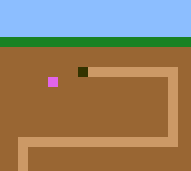
\includegraphics[height=8cm]{../img/blockworm}
%
\includegraphics[height=4cm]{../img/java-logo.png}
%
\includegraphics[height=12cm]{cover/gurka.jpg}
\vspace{2cm}
}

\author{Björn Regnell}
\date{\raggedbottom%
\vspace{1em}\begin{minipage}{1.0\textwidth}\centering
EDAA45, Lp1-2, HT \CurrentYear\\
Datavetenskap, LTH\\
Lunds universitet\\
~\\
Kompileringsdatum: \today \\
\url{http://cs.lth.se/pgk}
\end{minipage}
}

\usepackage{multicol}

\usepackage{pgffor}  %% http://stackoverflow.com/questions/2561791/iteration-in-latex
                     %  allows:  \foreach \n in {1,...,4}{ do something with \n }

\usepackage{framed}  %  allows:   \begin{framed}\end{framed}
\FrameSep5pt
\OuterFrameSep0pt

% \newenvironment{Slide}[2][]{%
% \begin{oframed}\setlist{noitemsep}%
% {\vspace{-1.5\topsep}}%tighter frames
% \subsection{#2}%
% }%
% {\end{oframed}}

\newenvironment{Slide}[2][]{%
%\noindent\rule{\textwidth}{0.4pt}%
\setlist{noitemsep}%
%{\vspace{-1.5\topsep}}%tighter frames
\subsection{#2}%
}%
{~\newline\noindent\rule{\textwidth}{0.4pt}}

%\newenvironment{Slide}[2][]{\setlist{noitemsep}\subsection{#2}}{}


%\newcommand{\SlideHeading}[1]{\section*{#1}}

%\usepackage[most]{tcolorbox}
% \newenvironment{Slide}[2][]
%   {\vspace{0.5em}\begin{tcolorbox}[left=1.5em,%width=1.05\textwidth,
%   grow to right by=0.05\textwidth,grow to left by=0.05\textwidth,%
%   %breakable,
%   %frame hidden,
%   colframe=gray!20,
%   enhanced]\setlist{noitemsep}\SlideHeading{#2}}
%   {\end{tcolorbox}\vspace{0.5em}}

\newcommand{\Subsection}[1]{} %ignore slide sections
\newcommand{\SlideOnly}[1]{} %ignore slide font size

\usepackage[framemethod=tikz]{mdframed}

\newif\ifkompendium  % to allow conditional text in slides only showing up in compendium
\kompendiumtrue      % in slides: \kompendiumfalse

\newif\ifPreSolution  % to allow tasks and solutions in same file
\PreSolutiontrue      % in solutions: \PreSolutionfalse

\let\QUESTBEGIN\ifPreSolution  % to mark formatting and numbering of exercises
\let\SOLUTION\else  % to mark solutions in the same file as questions
\let\QUESTEND\fi    % to mark end of exercise


%!TEX encoding = UTF-8 Unicode

\newcommand{\ModWeekONE}{Introduktion}
\newcommand{\ExeWeekONE}{expressions}
\newcommand{\LabWeekONE}{kojo}


\newcommand{\ModWeekTWO}{Program, kontrollstrukturer}
\newcommand{\ExeWeekTWO}{programs}
\newcommand{\LabWeekTWO}{--}


\newcommand{\ModWeekTHREE}{Funktioner, abstraktion}
\newcommand{\ExeWeekTHREE}{functions}
\newcommand{\LabWeekTHREE}{irritext}


\newcommand{\ModWeekFOUR}{Objekt, inkapsling}
\newcommand{\ExeWeekFOUR}{objects}
\newcommand{\LabWeekFOUR}{blockmole}


\newcommand{\ModWeekFIVE}{Klasser, datamodellering}
\newcommand{\ExeWeekFIVE}{classes}
\newcommand{\LabWeekFIVE}{--}


\newcommand{\ModWeekSIX}{Mönster, felhantering}
\newcommand{\ExeWeekSIX}{patterns}
\newcommand{\LabWeekSIX}{blockbattle}


\newcommand{\ModWeekSEVEN}{Sekvenser, enumerationer}
\newcommand{\ExeWeekSEVEN}{sequences}
\newcommand{\LabWeekSEVEN}{shuffle}


\newcommand{\ModWeekEIGHT}{Matriser, typparametrar}
\newcommand{\ExeWeekEIGHT}{matrices}
\newcommand{\LabWeekEIGHT}{life}


\newcommand{\ModWeekNINE}{Mängder, tabeller}
\newcommand{\ExeWeekNINE}{lookup}
\newcommand{\LabWeekNINE}{words}


\newcommand{\ModWeekTEN}{Arv, komposition}
\newcommand{\ExeWeekTEN}{inheritance}
\newcommand{\LabWeekTEN}{snake0}


\newcommand{\ModWeekELEVEN}{Kontextuella abstraktioner, api}
\newcommand{\ExeWeekELEVEN}{context}
\newcommand{\LabWeekELEVEN}{snake1}


\newcommand{\ModWeekTWELVE}{Valfri fördjupning, Projekt}
\newcommand{\ExeWeekTWELVE}{extra}
\newcommand{\LabWeekTWELVE}{Projekt0}


\newcommand{\ModWeekTHIRTEEN}{Repetition}
\newcommand{\ExeWeekTHIRTEEN}{examprep}
\newcommand{\LabWeekTHIRTEEN}{Projekt1}


\newcommand{\ModWeekFOURTEEN}{Muntligt prov}
\newcommand{\ExeWeekFOURTEEN}{Munta}
\newcommand{\LabWeekFOURTEEN}{Munta}


\begin{document}

\pagenumbering{roman}

\frontmatter
\maketitle
%!TEX encoding = UTF-8 Unicode
%!TEX root = ../compendium.tex

\clearpage\null\thispagestyle{empty}
\vfill

{
\setlength{\parindent}{0pt}
\emph{Editor}: Björn Regnell \\

%  LIST OF CONTRIBUTORS to https://github.com/lunduniversity/introprog
%    Please contact bjorn.regnell@cs.lth.se if you think you should be
%    on this list, or make a pull request with an update of file briefly
%    describing your contribtion in the commit text.
%    This work is licenced under CC-BY-SA-4.0.
%!TEX encoding = UTF-8 Unicode
%!TEX root = compendium/compendium.tex
\hyphenation{Borg-lund Da-ne-bjer Grampp Palm-qvist Ravn-borg Ro-sen-qvist Schrei-ter Wih-lan-der}
\emph{Contributors} in alphabetical order:
Anders Buhl,
André Philipsson Eriksson,
Anna Axelsson,
Anna Palmqvist Sjövall,
Anton Andersson,
Benjamin Lindberg,
Björn Regnell,
Casper Schreiter,
Cecilia Lindskog,
Dag Hemberg,
Elliot Bräck,
Elsa Cervetti Ogestad,
Emelie Engström,
Emil Wihlander,
Erik Bjäreholt,
Erik Grampp,
Evelyn Beck,
Fredrik Danebjer,
Gustav Cedersjö,
Henrik Olsson,
Hussein Taher,
Jakob Hök,
Jakob Sinclair,
Johan Ravnborg,
Jonas Danebjer,
Jos Rosenqvist,
Maj Stenmark,
Maria Kulesh,
Måns Magnusson,
Nicholas Boyd Isacsson,
Niklas Sandén,
Oliver Persson,
Oscar Sigurdsson,
Oskar Berg,
Oskar Widmark,
Patrik Persson,
Per Holm,
Philip Sadrian,
Sandra Nilsson,
Sebastian Hegardt,
Simon Persson,
Stefan Jonsson,
Theodor Lundqvist,
Tim Borglund,
Tom Postema,
Valthor Halldorsson,
Viktor Claesson,
Wilhelm Wanecek,
William Karlsson.

\\ \newline

\emph{Home}: \url{https://cs.lth.se/pgk} \newline

\emph{Repo}: \url{https://github.com/lunduniversity/introprog} \\ \newline

This compendium is on-going work. \\ \textbf{Contributions are welcome!} \\
\emph{Contact}: \url{bjorn.regnell@cs.lth.se}
\\ \newline

%\emph{Cover art}: Björn Regnell (inspired by Poul Ströyer's illustration of Lennart Hellsing's lyrics to  the childrens song ''Herr Gurka'' with music by Knut Brodin)\\ \newline

~\\ \newline

You can use this work if you respect this \emph{LICENCE}: CC BY-SA 4.0 \\
\url{http://creativecommons.org/licenses/by-sa/4.0/} \\
Please do \emph{not} distribute your solutions to lab assignments and projects.
\\ \newline
Copyright \copyright~ 2015-2017. \\
Dept. of Computer Science, LTH, Lund University. Lund. Sweden.\\
}

%!TEX encoding = UTF-8 Unicode
%!TEX root = ../compendium.tex

\ChapterUnnum{Framstegsprotokoll} 


\subsubsection*{Genomförda övningar}

\vspace{1em}\noindent 
{Till varje laboration hör en övning med uppgifter som utgör förberedelse inför labben. Du behöver minst behärska grundövningarna för att klara labben inom rimlig tid. Om du känner att du behöver öva mer på grunderna, gör då även extrauppgifterna. Om du vill fördjupa dig, gör fördjupningsuppgifterna som är på mer avancerad nivå. Kryssa för nedan vilka övningar du har gjort, så blir lätt för din handledare att se vilka kunskaper du förvärvat hittills.}

\newcommand{\TickBox}{\raisebox{-.50ex}{\Large$\square$}}
\newcommand{\ExeRow}[1]{\texttt{#1} & \TickBox  &  \TickBox &  \TickBox  \\ \addlinespace }

\begin{table}[h]
\centering
\vspace{2em}
\begin{tabular}{lccc}
\toprule \addlinespace 
{\sffamily\small Övning} & 
{\sffamily\small Grund} &	
{\sffamily\small Extra} &
{\sffamily\small Fördjupning}\\ \addlinespace \midrule \\[-0.7em]
\ExeRow{expressions}
\ExeRow{statements}
\ExeRow{functions}
\ExeRow{data}
\ExeRow{vectors}
\ExeRow{classes}
\ExeRow{traits}
\ExeRow{matching}
\ExeRow{matrices}
\ExeRow{sorting}
\ExeRow{scalajava}
\ExeRow{threads}
\bottomrule
\end{tabular}
\end{table}

\newpage

\subsubsection*{Godkända obligatoriska moment}

\vspace{1em}\noindent 
För att bli godkänd på laborationsuppgifterna och projektuppgiften måste du lösa deluppgifterna och diskutera dina lösningar med en handledare. Denna diskussion är din möjlighet att få feedback på dina lösningar. Ta vara på den!
Se till att handledaren noterar nedan när du blivit godkänd på respektive labb. Spara detta blad tills du fått slutbetyg i kursen. 


\vspace{2.5em}\noindent Namn: \dotfill\\

\vspace{1em}\noindent Namnteckning: \dotfill\\

\newcommand{\LabRow}[1]{\\[-1.1em] \texttt{#1} & \dotfill &  \dotfill  \\ \addlinespace }

\begin{table}[h]
\centering
\vspace{1em}
\begin{tabular}{lcc}
\toprule \addlinespace 
{\sffamily\bfseries\small Lab} & {\sffamily\small Datum gk} &	{\sffamily\small Handledares namnteckning}\\ \addlinespace \midrule \\[-0.5em]
%!TEX encoding = UTF-8 Unicode
%!TEX root = ../compendium2.tex
\LabRow{kojo}
\LabRow{irritext}
\LabRow{blockmole}
\LabRow{blockbattle}
\LabRow{shuffle}
\LabRow{words}
\LabRow{life}
\LabRow{snake}
\LabRow{music}
\LabRow{javatext}
\LabRow{survey}
%\toprule 
\addlinespace \midrule \addlinespace
 \\
{\sffamily\small {\bfseries Projektuppgift} (välj en)	} & \dotfill&\dotfill \\ \addlinespace\addlinespace %\midrule
\texttt{( ) bank}  &  &  \\
\texttt{( ) imageprocessing}  \\
\texttt{( ) tictactoe} \\  
\texttt{( ) }\textit{egendefinerad}  \\
\textit{\small Om egen, ge kort beskrivning:}\\
%\dotfill  \\
\bottomrule
\end{tabular}
\end{table}
%!TEX root = ../compendium.tex


\ChapterUnnum{Förord} 

Programmering är inte bara ett sätt att ta makten över systemen som styr vårt samhälle. Det är också ett kraftfullt verktyg för tanken. Att lära sig programmering och systemutveckling är första steget på en livslång resa av kontinuerligt lärande. Programmeringsspråk och utvecklingsverktyg kommer och går, men de grundläggande koncepten sekvens, alternativ, repetition och abstraktion som ligger bakom all mjukvara består. 

Detta kompendium utgör kursmaterial för studier i grundläggande programmering, med syfte att ge en solid bas för ingenjörsstudenter och andra som utvecklar system som innehåller mjukvara. 

Kompendiet är framtaget av, med och för studenter och lärare på universitetsnivå, och distribueras som öppen källkod. Det får användas fritt så länge erkännande ges och eventuella ändringar också publiceras som öppen källkod under samma licens som ursprungsmaterialet. På kursens hemsida \href{http://cs.lth.se/pgk}{cs.lth.se/pgk} och repo \href{http://github.com/lunduniversity/introprog}{github.com/lunduniversity/introprog} finns instruktioner om hur du kan bidra till kursmaterialet.

Läromaterialet fokuserar på lärande genom eget arbete och innehåller övningar och laborationer som är organiserade i moduler. Varje modul har ett tema och tillhörande föreläsningsanteckningar.

I kursen används språken Scala och Java för att illustrera grunderna i imperativ och objektorienterad programmering, tillsammans med elementär funktionsprogrammering. Mer avancerad objektorientering och funktionsprogrammering och  lämnas till fortsättningskurser. 



Den kanske viktigaste framgångsfaktorn vid studier i programmering är att bejaka din egen upptäckarglädje och experimentlusta. Det fantastiska med programmering är att dina egna intellektuella konstruktioner faktiskt \emph{gör} något som just \emph{du} har bestämt! Ta vara på det och prova dig fram genom att koda egna idéer -- det är kul när det funkar men minst lika lärorikt är felsökning, buggrättande och alla misslyckade försök som efter hårt arbete vänds till lyckade lösningar och bestående lärdomar. 

Välkommen i programmeringens fascinerande värld och hjärtligt lycka till med dina studier!




\setcounter{tocdepth}{2} % set headings level in table of contents

\tableofcontents
\mainmatter

\pagenumbering{arabic}


\part{Om kursen}
\setcounter{chapter}{-3}
%!TEX root = ../compendium.tex

\ChapterUnnum{Kursens arkitektur}
\begin{framed}
%\noindent\resizebox{\columnwidth}{!}{%
%!TEX encoding = UTF-8 Unicode
\begin{tabular}{l|l|l|l}
\textit{W} & \textit{Modul} & \textit{Övn} & \textit{Lab} \\ \hline \hline
W01 & Introduktion            & expressions & kojo            \\
W02 & Kodstrukturer           & programs    & --              \\
W03 & Funktioner, Objekt      & functions   & bugs            \\
W04 & Datastrukturer          & data        & pirates         \\
W05 & Sekvensalgoritmer       & sequences   & cards           \\
W06 & Klasser, Likhet         & classes     & turtlegraphics  \\
W07 & Arv, Gränssnitt         & traits      & turtlerace-team \\
KS  & KONTROLLSKRIVN.         & --          & --              \\
W08 & Mönster, Undantag       & matching    & chords-team     \\
W09 & Matriser, Typparametrar & matrices    & maze            \\
W10 & Sökning, Sortering      & sorting     & surveydata-team \\
W11 & Scala och Java          & scalajava   & lthopoly-team   \\
W12 & Trådar                  & threads     & life            \\
W13 & Design                  & Uppsamling  & Projekt         \\
W14 & Tentaträning            & Extenta     & --              \\
T   & TENTAMEN                & --          & --              \\
\end{tabular}

%}
\end{framed}

Kursen består av ett antal moduler med tillhörande teori, övningar och laborationer. Genom att göra övningarna bearbetar du teorin och förebereder dig inför laborationerna. När du klarar laborationen i varje modul är du redo att gå vidare till efterkommande modul.  

\newcommand{\Subsection}[1]{} %ignore slide sections

\newenvironment{Slide}[2][]
  {\begin{framed}\setlist{noitemsep}\section*{#2}}
  {\end{framed}}

\newif\ifkompendium
\kompendiumtrue

%!TEX root = ../lect-week01.tex

%%%%%%%%%%%%%%%%%%%%%%%%%%%%%%%%%%%%%%
\Subsection{Om denna kurs}

%%%
\begin{Slide}{Vad och hur?}
\begin{itemize}
\item \emph{Vad} ska du lära dig?
\begin{itemize}
\item Grundläggande principer för programmering\\ $\implies$Inga förkunskaper i programmering krävs!
\item Konstruktion av algoritmer
\item Tänka i abstraktioner
\item Flera olika angreppsätt: imperativ programmering, objektorientering, funktionsprogrammering
\item Programspråken Scala och Java
\item Utvecklingsverktyg (editor, kompilator, utvecklingsmiljö)
\item Implementera, testa, felsöka
\end{itemize}

\item \emph{Hur} ska du lära dig?
\begin{itemize}
\item Genom praktiskt eget arbete: \Emph{Lära genom att göra!}
\item Genom studier av kursens teori: \Emph{Skapa förståelse!}
\item Genom samarbete med dina kurskamrater: \Emph{Gå djupare!}
\end{itemize}
\end{itemize}
\end{Slide}


\ifkompendium
\subsection{hej}
Denna text hamnar bara i kompediet

Hejsan svejsan

\begin{itemize}
\item some item
\end{itemize}


\begin{Code}
hej kod
\end{Code}
\fi


\ifkompendium\else
\begin{Slide}{TESTSLAJD EJ I KOMPENDIUM}
\begin{itemize}
\item \emph{Hej} på dig
\item blablab
\item blabla
\end{itemize}
\begin{Code}
hej kod
\end{Code}
\end{Slide}
\fi


%%%%%%%%%%%%%%%%%%%%%%%%%%%%%%%%%%%%%%
\ifkompendium\else
\Subsection{Meddelande från \href{http://lth.se/code}{Code@LTH}} 
\fi

\begin{itemize}
\item item
\item item
\item item
\item item
\end{itemize}


%!TEX encoding = UTF-8 Unicode
%!TEX root = ../compendium.tex

\ChapterUnnum{Anvisningar}

\SectionUnnum{Samarbetsgrupper}
\subsection*{Samarbetskontrakt}
\subsection*{Grupplaborationer}
\subsection*{Samarbetsbonus}
\SectionUnnum{Föreläsningar}
\SectionUnnum{Övningar}
\SectionUnnum{Laborationer}
 
\begin{itemize}
\item TODO!!! Skriv om pennan och ögat och bocken
\item TODO!!! Skriv att om man inte gör föreberedelserna hinner man inte labben på 2h
\end{itemize}
\SectionUnnum{Resurstider}
\SectionUnnum{Kontrollskrivning}
\SectionUnnum{Tentamen}
%!TEX encoding = UTF-8 Unicode
%!TEX root = ../compendium.tex


\ChapterUnnum{Hur bidra till kursmaterialet?}

%\renewcommand{\SlideHeading}[1]{\subsection{#1}}  %numbering sections in compendium slides

\part{Moduler}

  %remove space before subsection
  %https://stackoverflow.com/questions/3191640/heading-subsection-at-start-of-framed-environment-in-latex-without-leading-padd


%!TEX encoding = UTF-8 Unicode
%!TEX root = ../compendium1.tex

\renewcommand{\vecka}{1}

\chapter{Introduktion}\label{chapter:W01}
\begin{itemize}[nosep]
\item sekvens
\item alternativ
\item repetition
\item abstraktion
\item programmeringsspråk
\item programmeringsparadigmer
\item editera-kompilera-exekvera
\item datorns delar
\item virtuell maskin
\item värde
\item uttryck
\item variabel
\item typ
\item tilldelning
\item namn
\item val
\item var
\item def
\item if
\item else
\item true
\item false
\item MinValue
\item MaxValue
\item aritmetik
\item slumptal
\item math.random
\item logiska uttryck
\item de Morgans lagar
\item while-sats
\item for-sats
\end{itemize}
\clearpage

%!TEX encoding = UTF-8 Unicode
%!TEX root = ../lect-w01.tex

%%%%%%%%%%%%%%%%%%%%%%%%%%%%%%%%%%%%%%

\Subsection{Att lära denna läsvecka \texttt{w01}}

\ifkompendium\else  %%%%%%%%%%%%%%%%%%%%%%%%%%%%%%%%%%%%%%%%%%%%%%%%%
\begin{SlideExtra}{Att lära denna läsvecka \texttt{w01}}
%!TEX encoding = UTF-8 Unicode

    Modul \Emph{Introduktion}: Övn \Alert{\texttt{expressions}} $\rightarrow$ Labb \Alert{\texttt{kojo}}
    \begin{multicols}{3}\SlideFontTiny
    $\square$ sekvens \\
$\square$ alternativ \\
$\square$ repetition \\
$\square$ abstraktion \\
$\square$ editera \\
$\square$ kompilera \\
$\square$ exekvera \\
$\square$ datorns delar \\
$\square$ virtuell maskin \\
$\square$ litteral \\
$\square$ värde \\
$\square$ uttryck \\
$\square$ identifierare \\
$\square$ variabel \\
$\square$ typ \\
$\square$ tilldelning \\
$\square$ namn \\
$\square$ val \\
$\square$ var \\
$\square$ def \\
$\square$ definera och anropa funktion \\
$\square$ funktionshuvud \\
$\square$ funktionskropp \\
$\square$ procedur \\
$\square$ inbyggda grundtyper \\
$\square$ Int \\
$\square$ Long \\
$\square$ Short \\
$\square$ Double \\
$\square$ Float \\
$\square$ Byte \\
$\square$ Char \\
$\square$ String \\
$\square$ println \\
$\square$ typen Unit \\
$\square$ enhetsvärdet () \\
$\square$ stränginterpolatorn s \\
$\square$ if \\
$\square$ else \\
$\square$ true \\
$\square$ false \\
$\square$ MinValue \\
$\square$ MaxValue \\
$\square$ aritmetik \\
$\square$ slumptal \\
$\square$ math.random \\
$\square$ logiska uttryck \\
$\square$ de Morgans lagar \\
$\square$ while-sats \\
$\square$ for-sats \\
    \end{multicols}
    
\end{SlideExtra}
\fi

\Subsection{Om programmering}

\ifkompendium\else  %%%%%%%%%%%%%%%%%%%%%%%%%%%%%%%%%%%%%%%%%%%%%%%%%

\begin{SlideExtra}{Att skapa koden som styr världen}
\begin{multicols}{2}\footnotesize
I stort sett \Alert{alla} delar av samhället är beroende av programkod:
\begin{itemize}\scriptsize
\item kommunikation
\item transport
\item byggsektorn
\item statsförvaltning
\item finanssektorn
\item media \& underhållning
\item sjukvård
\item övervakning
\item integritet
\item upphovsrätt
\item miljö \& energi
\item sociala relationer
\item utbildning
\item ...
\end{itemize}
\columnbreak %---------
Hur blir ditt framtida yrkesliv som systemutvecklare?
\begin{itemize}
\item  Det är sedan lång tid en \Alert{skriande brist} på utvecklare och det blir bara värre... \\
\href{https://cio.idg.se/2.1782/1.710012/kompetenslarm-jobb-om-fem-ar?queryText=kompetensbrist}{CIO 2018-11-09} %\\
%\href{http://computersweden.idg.se/2.2683/1.663879/oppen-kallkod-brist-kompetens}{CS 2016-08-23} 

\item Störst brist är det på \Emph{kvinnliga} utvecklare: \\
\href{https://www.svt.se/nyheter/inrikes/stor-brist-pa-programmerare-kvinnor-lockas-till-yrket}{SVT 2016-12-03}

\item Global kompetensmarknad \\
  \href{https://cio.idg.se/2.1782/1.648294/hitta-it-kompetens/sida/2/global-rekrytering-aktivt-hr-arbete}{CIO 2016-02-01}\\
  \href{http://computersweden.idg.se/2.2683/1.630901/det-finns-programmerare-och-sa-finns-det-programmerare}{CS 2015-06-14} \\
  \href{http://computersweden.idg.se/2.2683/1.662186/25-miljoner-utvecklare?queryText=miljoner\%20utvecklare}{CS 2016-07-14 }
\end{itemize}
\end{multicols}

\end{SlideExtra}

\begin{SlideExtra}{Utveckling av mjukvara i praktiken}
\begin{itemize}
\item \Emph{Inte bara kodning:} kravbeslut, releaseplanering, design, test, versionshantering, kontinuerlig integration, driftsättning, återkoppling från dagens användare, ekonomi \& investering, gissa om morgondagens användare, ...
\item \Emph{Teamwork:} Inte ensamma hjältar utan autonoma team i decentraliserade organisationer med innovationsuppdrag
\item \Emph{Snabbhet:} Att koda innebär att hela tiden uppfinna nya ''byggstenar'' som ökar organisationens förmåga att snabbt skapa värde med hjälp av mjukvara. \Alert{Öppen källkod}. Skapa kraftfulla API:er.
\item \Emph{Livslångt lärande:} Lär nytt och dela med dig hela tiden. Exempel på pedagogisk utmaning: hjälp andra förstå och använda ditt API $\implies$ \Alert{Samarbetskultur}
\end{itemize}
\end{SlideExtra}


\fi %%%%%%%%%%%%%%%%%%%%%%%%%%%%%%%%%%%%%%%%%%%%%%%%%%%%


% \ifkompendium\else
% \SlideImg{Programming unplugged: Två frivilliga?}{../img/unplugged}
% \SlideImg{Editera och exekvera ett program}{../img/kojo}
% \fi

%%%

\ifkompendium\else
\SlideImg{Vad är en dator?}{../img/eniac}
\fi

\begin{Slide}{Hur fungerar en dator?}
\begin{tikzpicture}[node distance=2.0cm]
\node (input)  [startstop]               {Indata-enhet};
\node (cpu)    [process, below of=input] {CPU};
\node (output) [startstop,below of=cpu]  {Utdata-enhet};

\node (mem) [right of=cpu, xshift=0.4\textwidth, draw = black, thick] {
\begin{minipage}{0.5\textwidth}\centering
\textbf{Minne} med minnesceller
\vspace{1em}

\begin{tabular}{|l | l|}
address & innehåll \\ \hline
0   & 42 \\ \hline
1   & 13 \\ \hline
2   & 18 \\ \hline
3   & 21 \\ \hline
4   & 55 \\ \hline
5   & 64 \\ \hline
6   & 48 \\ \hline
... & ...
\end{tabular}
\end{minipage}
};

\draw [arrow] (input) -- (cpu);
\draw [arrow] (cpu) -- (output);
\draw [arrow] (cpu) -- (mem);
\draw [arrow] (mem) -- (cpu);

\end{tikzpicture}

{\hfill
\begin{minipage}{0.65\textwidth}\vspace{1em}
Minnet innehåller endast \Alert{heltal} som \newline representerar \Emph{data} \Alert{och} \Emph{instruktioner}.
\end{minipage}
}
\end{Slide}

\begin{Slide}{Vad är programmering?}
\begin{itemize}
\item Programmering innebär att ge instruktioner till en maskin.
\item Ett \Emph{programmeringsspråk} används av människor för att skriva \Emph{källkod} som kan översättas av en \Emph{kompilator} till \Emph{maskinspråk} som i sin tur \Emph{exekveras} av en dator.
\end{itemize}


\begin{minipage}{.8\textwidth}
\begin{itemize}
\item Ada Lovelace publicerade det första programmet redan på 1800-talet ämnat för en kugghjulsdator.
\end{itemize}
\end{minipage}%
\begin{minipage}{.2\textwidth}
\centering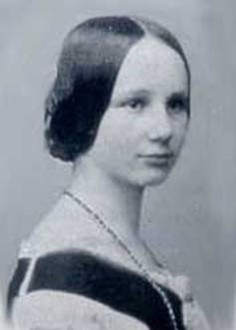
\includegraphics[width=0.6\columnwidth]{../img/ada}
\end{minipage}%
\begin{itemize}
\item \href{https://sv.wikipedia.org/wiki/Programmering}{sv.wikipedia.org/wiki/Programmering}
\item \href{https://en.wikipedia.org/wiki/Computer\_programming}{en.wikipedia.org/wiki/Computer\_programming}
\item Ha picknick i \href{http://kartor.lund.se/wiki/lundanamn/index.php/Ada_Lovelace-parken}{Ada Lovelace-parken} på Brunnshög!
\end{itemize}
\end{Slide}


\begin{Slide}{Vad är en kompilator?}
\begin{minipage}{.35\textwidth}
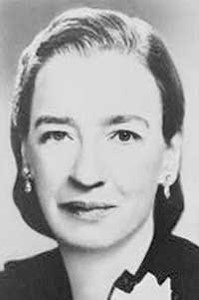
\includegraphics[width=0.6\textwidth]{../img/grace}
\end{minipage}%
\begin{minipage}{.67\textwidth}
%https://www.sharelatex.com/blog/2013/08/29/tikz-series-pt3.html
\begin{tikzpicture}[node distance=1.4cm,scale=0.8]
  \node (input) [startstop] {Källkod};
  \node(inptext) [right of=input, text width=2cm, scale=0.8,xshift=1.5cm]{För\\människor};
  \node (compile) [process, below of=input] {Kompilator};
  \node (output) [startstop, below of=compile] {Maskinkod};
  \node(outtext) [right of=output, text width=2cm, scale=0.8,xshift=1.5cm]{För\\maskiner};
  \draw [arrow] (input) -- (compile);
  \draw [arrow] (compile) -- (output);
  \end{tikzpicture}%

\vspace{1em}\noindent Grace Hopper uppfann kompilatorn 1952. \\ \href{https://en.wikipedia.org/wiki/Grace\_Hopper}{\SlideFontTiny en.wikipedia.org/wiki/Grace\_Hopper}
\end{minipage}%
\end{Slide}


\begin{Slide}{Virtuell maskin (VM) == abstrakt hårdvara}
\begin{multicols}{2}
\begin{itemize}
\item En VM är en ''dator'' implementerad i mjukvara som kan tolka en generell ''maskinkod'' som \Emph{översätts under körning} till den \Alert{verkliga} maskinens specifika maskinkod.

\item Med en VM blir källkoden \Emph{plattformsoberoende} och fungerar på många olika maskiner.

\item Exempel JVM: \\ \Emph{Java Virtual Machine}


\end{itemize}

\columnbreak %---------

%https://www.sharelatex.com/blog/2013/08/29/tikz-series-pt3.html
\begin{tikzpicture}[node distance=1.4cm]
\node (input) [startstop] {Källkod};
\node (compile) [process, below of=input] {Kompilator};
\node (output) [startstop, below of=compile] {Generell ''maskinkod''};
\node (interp) [process, below of=output] {VM interpreterar};
\node (output2) [startstop, below of=interp] {Specifik maskinkod};
\draw [arrow] (input) -- (compile);
\draw [arrow] (compile) -- (output);
\draw [arrow] (output) -- (interp);
\draw [arrow] (interp) -- (output2);
\end{tikzpicture}
\end{multicols}
\end{Slide}

\begin{Slide}{Vad består ett program av?}
\begin{itemize}
\item Text som följer entydiga språkregler (grammatik):
\begin{itemize}
\item \Emph{Syntax}: textens konkreta utseende
\item \Emph{Semantik}: textens betydelse (vad maskinen gör/beräknar)
\end{itemize}
\item \Emph{Nyckelord}: ord med speciell betydelse, t.ex. \code{if}, \code{else}
\item \Emph{Deklarationer}: definitioner av nya ord: \code{def gurka = 42}
\item \Emph{Satser} är instruktioner som \Alert{gör} något: \code{print("hej")}
\item \Emph{Uttryck} är instruktioner som beräknar ett \Alert{resultat}: \code{1 + 1}
\item \Emph{Data} är information som behandlas: t.ex. heltalet \code{42}
\item Instruktioner ordnas i kodstrukturer: \Alert{SARA}
\begin{itemize}
  \item \Emph{Sekvens}: ordningen spelar roll för vad som händer
  \item \Emph{Alternativ}: olika resultat beroende på uttrycks värde
  \item \Emph{Repetition}: instruktioner upprepas många gånger
  \item \Emph{Abstraktion}: nya byggblock skapas för att återanvändas
\end{itemize}
\end{itemize}
\end{Slide}

\begin{Slide}{Exempel på programmeringsspråk}
Det finns massor med olika språk och det kommer ständigt nya.
\vspace{1em}
\begin{multicols}{2}
Exempel:
\begin{itemize}
\item Java
\item C
\item C++
\item C\#
\item Python
\item JavaScript
\item Scala
\end{itemize}

\columnbreak %---------

Topplistor:
\begin{itemize}
\item \href{https://redmonk.com/sogrady/2020/07/27/language-rankings-6-20/}{Redmonk language rankings}   
%\item \href{https://redmonk.com/sogrady/2019/07/18/language-rankings-6-19/}{Redmonk language rankings}   
%\item \href{https://redmonk.com/sogrady/2018/08/10/language-rankings-6-18/}{Redmonk language rankings}   
\item \href{http://pypl.github.io/PYPL.html}{PYPL Index}
\item \href{http://www.tiobe.com/index.php/content/paperinfo/tpci/index.html}{TIOBE Index}
\end{itemize}
% \vspace{1em}
% 
\includegraphics[width=0.8\columnwidth]{../img/pypl}\\\SlideFontSmall{[PYPL (2016)]}
\end{multicols}

\end{Slide}

\ifkompendium\else
\begin{SlideExtra}{Redmonk Language Rankings: Github, Stackoverflow}
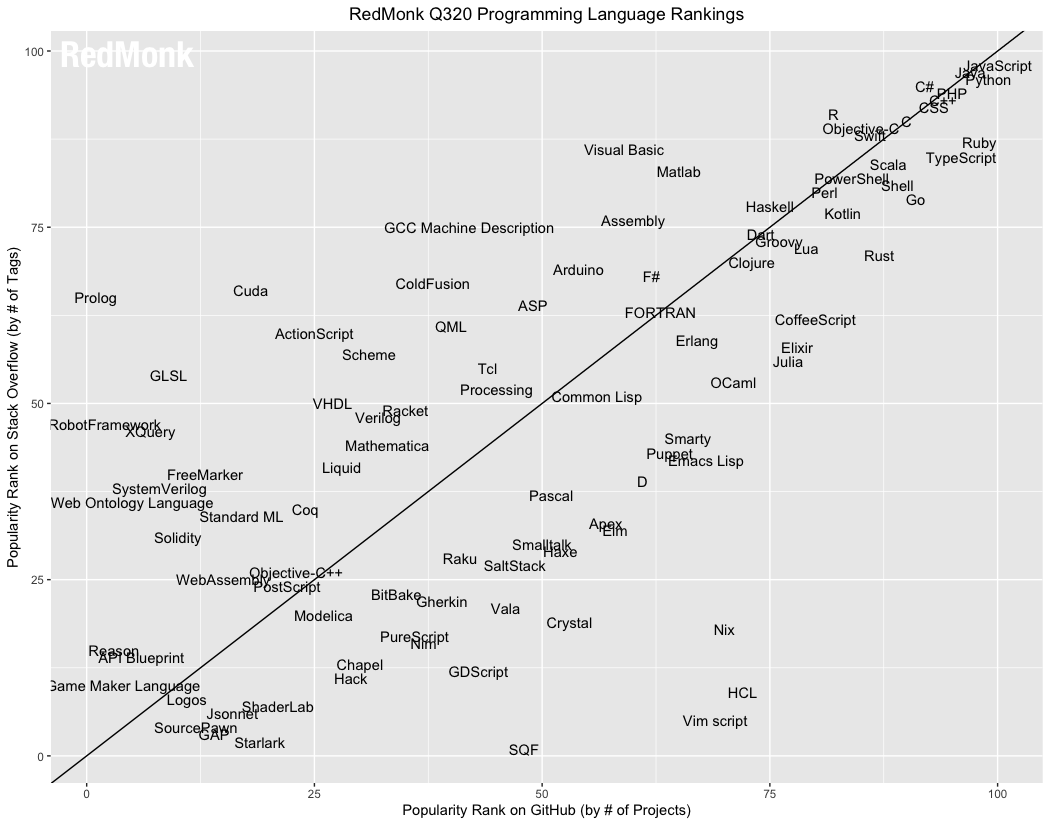
\includegraphics[width=0.95\columnwidth]{../img/redmonk-Q320}
\end{SlideExtra}
\begin{SlideExtra}{Några språks utveckling över tid enl. PYPL}
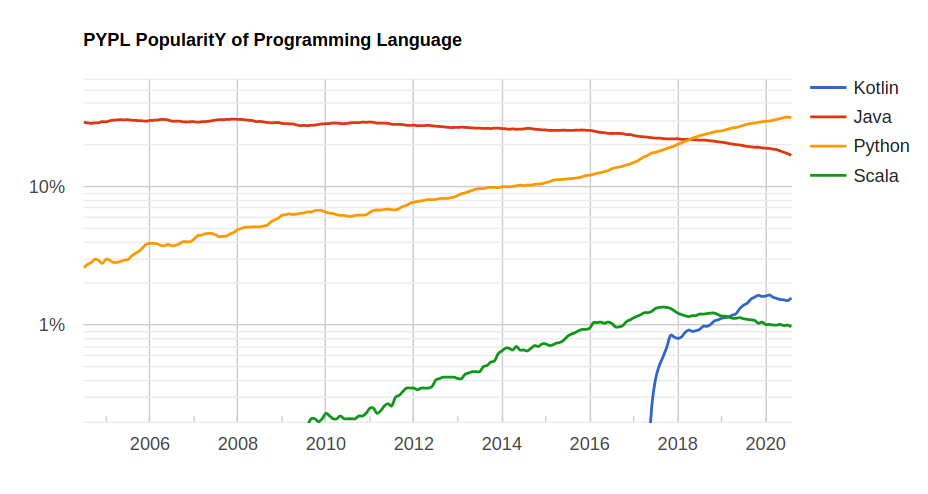
\includegraphics[width=0.95\columnwidth]{../img/pypl-06-20}
\end{SlideExtra}

\fi

\begin{Slide}{Olika programmeringsparadigm}
\begin{itemize}
\item Det finns många olika \href{https://en.wikipedia.org/wiki/Programming_paradigm}{programmeringsparadigm} (sätt att programmera på), till exempel:
\begin{itemize}\SlideFontSmall
\item \Emph{imperativ programmering:} programmet är uppbyggt av sekvenser av olika satser som påverkar systemets tillstånd
\item \Emph{objektorienterad programmering:} en sorts imperativ programmering där programmet består av objekt som sammanför data och operationer på dessa data
\item \Emph{funktionsprogrammering:} programmet är uppbyggt av samverkande (matematiska) funktioner som undviker föränderlig data och tillståndsändringar
\item \Emph{deklarativ programmering, logikprogrammering:} programmet är uppbyggt av logiska uttryck som beskriver olika fakta eller villkor och exekveringen utgörs av en bevisprocedur som söker efter värden som uppfyller fakta och villkor
\end{itemize}
\end{itemize}
\end{Slide}


\begin{Slide}{Hello world}

Scala-skript:
\begin{REPLnonum}
scala> println("Hello World!")
Hello World!
\end{REPLnonum}

Scala-applikation:
\begin{Code}
object Hello {
  def main(args: Array[String]): Unit = println("Hello world!")
}
\end{Code}

Java-applikation:
\begin{Code}[language=Java]
public class Hello {
    public static void main(String[] args) {
        System.out.println("Hello world!");
    }
}
\end{Code}

\end{Slide}

\begin{Slide}{Utvecklingscykeln}
editera; kompilera; hitta fel och förbättringar; editera; kompilera; hitta fel och förbättringar; editera; kompilera; hitta fel och förbättringar; editera; kompilera; hitta fel och förbättringar; editera; kompilera; hitta fel och förbättringar; editera; kompilera; hitta fel och förbättringar; ...

\begin{Code}
upprepa(1000){
  editera
  kompilera
  testa
}
\end{Code}
\end{Slide}

\begin{Slide}{Utvecklingsverktyg}
\begin{itemize}
\item Din verktygskunskap är mycket viktig för din produktivitet.
\item Lär dig kortkommandon för vanliga handgrep.
\item Verktyg vi använder i kursen:
\begin{itemize}
\item Scala \Emph{REPL}: från övn 1
\item \Emph{Texteditor} för kod, t.ex VS \code{code}: från övn 2
\item Kompilera med \Emph{\code{scalac}} och \Emph{\code{javac}}: från övn 2
\item Integrerad utvecklingsmiljö (IDE)
\begin{itemize}
\item \Emph{Kojo}: från lab 1
\item \Emph{IntelliJ IDEA} (alt. ScalaIDE/Eclipse): från läsperiod 2
\end{itemize}
\item \Emph{jar} för att packa ihop och distribuera klassfiler
\item \Emph{javadoc} och \Emph{scaladoc} för dokumentation av kodbibliotek
\end{itemize}
\item Andra verktyg som är bra att lära sig:
\begin{itemize}
\item git för versionshantering
\item GitHub för kodlagring -- men \Alert{inte} av lösningar till labbar!
\end{itemize}
\end{itemize}
\end{Slide}





\Subsection{De enklaste beståndsdelarna: litteraler, uttryck, variabler}


\begin{Slide}{Litteraler}
\begin{itemize}
\item En literal representerar ett fixt \Emph{värde} i koden och används för att skapa \Alert{data} som programmet ska bearbeta.
\item Exempel: \\
\begin{tabular}{l l}
\code|42| & heltalslitteral\\
\code|42.0| & decimaltalslitteral\\
\code|'!'| & teckenlitteral, omgärdas med 'enkelfnuttar' \\
\code|"hej"| & stränglitteral, omgärdas med ''dubbelfnuttar'' \\
\code|true| & litteral för sanningsvärdet ''sant''\\
\end{tabular}
\item Literaler har en \Emph{typ} som avgör vad man kan göra med dem.
\end{itemize}
\end{Slide}

\begin{Slide}{Exempel på inbyggda datatyper i Scala}\SlideFontSmall
\begin{itemize}
\item Alla värden, uttryck och variabler har en \href{https://sv.wikipedia.org/wiki/Datatyp}{\Emph{datatyp}}, t.ex.:
\begin{itemize}\footnotesize
\item \code{Int} för heltal
\item \code{Long} för \textit{extra} stora heltal (tar mer minne)
\item \code{Double} för decimaltal, så kallade flyttal med flytande decimalpunkt
\item \code{String} för strängar
\end{itemize}

\item Kompilatorn håller reda på att uttryck kombineras på ett \Emph{typsäkert} sätt. Annars blir det \Alert{kompileringsfel}.

\item Scala och Java är s.k. \href{https://sv.wikipedia.org/wiki/Typsystem}{\Emph{statiskt typade}} språk, vilket innebär att kontroll av typinformation sker vid kompilering \Eng{compile time}\footnote{Andra språk, t.ex. Python och Javascript är \Emph{dynamiskt typade} och där skjuts typkontrollen upp till körningsdags \Eng{run time} \\ Vilka är för- och nackdelarna med statisk vs. dynamisk typning?}.

\item Scala-kompilatorn gör \href{https://en.wikipedia.org/wiki/Type_inference}{\Emph{typhärledning}}: man \Alert{slipper skriva typerna} om kompilatorn kan lista ut dem med hjälp av typerna hos deluttrycken.

\end{itemize}
\end{Slide}


\begin{Slide}{Grundtyper i Scala}\SlideFontSmall
Dessa \Emph{grundtyper} \Eng{basic types} finns inbyggda i Scala:

\begin{table}[H]
\renewcommand{\arraystretch}{1.4}
\begin{tabular}{p{0.24\textwidth}|p{0.21\textwidth}|l}
\textit{Svenskt namn} & \textit{Engelskt namn} & \Emph{Grundtyper} \\ \hline
heltalstyp & integral type & \texttt{Byte}, \texttt{Short}, \texttt{Int}, \texttt{Long}, \texttt{Char} \\
flyttalstyp  &  floating point \newline number types & \texttt{Float}, \texttt{Double} \\
numeriska typer & numeric types & heltalstyper och flyttalstyper \\
strängtyp \newline (teckensekvens) & string type & \texttt{String}  \\
sanningsvärdestyp  \newline (boolesk typ)& truth value type & \texttt{Boolean} \\
\end{tabular}
\end{table}

\end{Slide}

\begin{Slide}{Grundtypernas implementation i JVM}\SlideFontSmall
\begin{table}[H]
\renewcommand{\arraystretch}{1.4}
\begin{tabular}{l|l|l|l}
\Alert{Grundtyp} i &  Antal                &      Omfång&\Alert{primitiv typ} i\\
 \Emph{Scala} & bitar & minsta/största värde &\Emph{Java} \& \Emph{JVM}\\ \hline
\texttt{Byte}   &  8  & $-2^7$ ... $2^7-1$   & \texttt{byte} \\
\texttt{Short}  &  16 & $-2^{15}$ ... $2^{15}-1$ & \texttt{short} \\
\texttt{Char}   &  16 & $0$ ... $2^{16}-1$ & \texttt{char} \\
\texttt{Int}    &  32 & $-2^{31}$ ... $2^{31}-1$ & \texttt{int} \\
\texttt{Long}   &  64 & $-2^{63}$ ... $2^{63}-1$ & \texttt{long} \\
\texttt{Float}  &  32 & ± $3.4028235 \cdot 10^{38}$  & \texttt{float} \\
\texttt{Double} &  64 & ± $1.7976931348623157 \cdot 10^{308}$ & \texttt{double} \\
\end{tabular}
\end{table}

Grundtypen \texttt{String} lagras som en \emph{sekvens} av 16-bitars tecken av typen \texttt{Char} och kan vara av godtycklig längd (tills minnet tar slut).

\end{Slide}


\begin{Slide}{Uttryck}
\begin{itemize}
\item Ett \Emph{uttryck} består av en eller flera delar som efter \Emph{evaluering} ger ett \Alert{resultat}.
\item Delar i ett uttryck kan t.ex. vara: \\ literaler (42), operatorer (+), funktioner (sin), ...
\item Exempel:
\begin{itemize}
\item Ett enkelt uttryck: \\ \code{42.0}
\item Sammansatta uttryck: \\
\code{40 + 2} \\
\code{(20 + 1) * 2} \\
\code{sin(0.5 * Pi)} \\
\code{"hej" + " på " + "dej"}
\end{itemize}

\item När programmet tolkas sker \Emph{evaluering} av uttrycket, vilket ger ett resultat i form av ett \Emph{värde} som har en \Emph{typ}.
\end{itemize}
\end{Slide}


\begin{Slide}{Variabler}\SlideFontSmall
\begin{itemize}
\item En \Emph{variabel} kan tilldelas värdet av ett enkelt eller sammansatt uttryck.
\item En variabel har ett \Emph{variabelnamn}, vars utformning följer språkets regler för s.k. \Emph{identifierare}.
\item En ny variabel införs i en \Emph{variabeldeklaration} och då den kan ges ett värde, \Emph{initialiseras}. Namnet användas som \Emph{referens} till värdet.
\item Exempel på variabeldeklarationer i Scala, notera \Emph{nyckelordet} \code{val}:
\begin{Code}
val a = 0.5 * Pi
val length = 42 * sin(a)
val exclamationMarks = "!!!"
val greetingSwedish = "Hej på dej" + exclamationMarks
\end{Code}

\item Vid exekveringen av programmet lagras variablernas värden i minnet och deras respektive värde hämtas ur minnet när de \Emph{refereras}.

\item Variabler som deklareras med \code{val} kan endast tilldelas ett värde \Alert{en enda gång}, vid den initialisering som sker vid deklarationen.
\end{itemize}

\end{Slide}


\begin{Slide}{Regler för identifierare}
\begin{itemize}
\item \Emph{Enkel} identifierare: t.ex. \code{gurka2tomat}
\begin{itemize}
\item Börja med bokstav
\item ...följt av bokstäver eller siffror
\item Kan även innehålla understreck
\end{itemize}

\item \Emph{Operator}-identifierare, t.ex. \code{+:}
\begin{itemize}
\item Börjar med ett \Emph{operatortecken}, t.ex. \code{+ - * / : ? ~ #}
\item Kan följas av fler operatortecken
\end{itemize}


\item En identifierare får \Alert{inte} vara ett \Emph{reserverat ord}, se \href{http://cs.lth.se/pgk/quickref}{snabbreferensen} för alla reserverade ord i Scala \& Java.

\item \Emph{Bokstavlig} identifierare: \code{`kan innehålla allt`}
\begin{itemize}
\item Börjar och slutar med \Emph{backticks}  \code{` `}
\item Kan innehålla vad som helst (utom backticks)
\item Kan användas för att undvika krockar med reserverade ord: \texttt{\code{`}val\code{`}}
\end{itemize}

\end{itemize}
\end{Slide}



%\begin{Slide}{Regler för identifierare i Java}\footnotesize
%När kompilatorn ''läser''  \footnote{man säger ofta ''parsa'' i stället för ''läsa'' när kompilatorn tolkar koden} koden och och försöker hitta variabelnamn, antar den att du följer de entydiga syntaktiska reglerna för språket.  \\ \vskip1em För namn i Java gäller följande regler: %https://docs.oracle.com/javase/tutorial/java/nutsandbolts/variables.html
%\begin{itemize}
%\item Namn får inte vara \href{https://docs.oracle.com/javase/tutorial/java/nutsandbolts/_keywords.html}{reserverade ord}
%\item Stora och små bokstäver spelar roll \Eng{case sensistive} \\ \lstinline{int highScore;} och \lstinline{int highscore;} ger alltså två \textit{olika} variabler
%\item Namnet måste börja med en bokstav, ett understreck \_ eller ett dollartecken \$
%\item Namn får \textit{inte} innehålla blanktecken
%\item Namn får innehålla bokstäver, siffror, understreck \_ och dollartecken \$, men \textit{inte} andra specialtecken (alltså inte \lstinline~%&@!{(})/+-*~ etc.)
%\end{itemize}
%\end{Slide}



\begin{Slide}{Att bygga strängar: konkatenering och interpolering}
\begin{itemize}
\item Man kan \Emph{konkatenera} strängar med operatorn + \\ \code{"hej" + " på " + "dej"}
\item Efter en sträng kan man konkatenera vilka uttryck som helst; uttryck inom parentes evalueras först och värdet görs sen om till en sträng före konkateneringen:
\begin{Code}
val x = 42
val msg = "Dubbla värdet av " + x + " är " + (x * 2) + "."
\end{Code}
\item Man kan i Scala (men inte Java) få hjälp av kompilatorn att övervaka bygget av strängar med \Emph{stränginterpolatorn} \Alert{s}:
\begin{Code}
val msg = s"Dubbla värdet av $x är ${x * 2}."
\end{Code}

\end{itemize}
\end{Slide}

\begin{Slide}{Heltalsaritmetik}\SlideFontSmall
\begin{itemize}
\item De fyra räknesätten skrivs som i matematiken (vanlig \href{https://en.wikipedia.org/wiki/Order_of_operations}{precedens}):
\begin{REPL}
scala> 3 + 5 * 2 - 1
res0: Int = 12
\end{REPL}
\item \Emph{Parenteser} styr \Alert{evalueringsordningen}:
\begin{REPL}
scala> (3 + 5) * (2 - 1)
res1: Int = 8
\end{REPL}
\item \Emph{Heltalsdivision} sker med \Alert{decimaler avkortade}:
\begin{REPL}
scala> 41 / 2
res2: Int = 20
\end{REPL}
\item \href{https://en.wikipedia.org/wiki/Modulo_operation}{\Emph{Moduloräkning}} med restoperatorn \code{%}
\begin{REPL}
scala> 41 % 2
res3: Int = 1
\end{REPL}
\end{itemize}
\end{Slide}


\begin{Slide}{Flyttalsaritmetik}\SlideFontSmall
\begin{itemize}
\item Decimaltal representeras med s.k. \href{https://sv.wikipedia.org/wiki/Flyttal}{\Emph{flyttal}} av typen \code{Double}:
\begin{REPL}
scala> math.Pi
res4: Double = 3.141592653589793
\end{REPL}

\item Stora tal så som $\pi*10^{12}$ skrivs:
\begin{REPL}
scala> math.Pi * 1E12
res5: Double = 3.141592653589793E12
\end{REPL}
\item Det finns \Alert{inte} oändligt antal decimaler vilket ger problem med \Alert{avvrundingsfel}:
\begin{REPL}
scala> 0.0000000000001
res6: Double = 1.0E-13

scala> 1E10 + 0.0000000000001
res7: Double = 1.0E10
\end{REPL}
\end{itemize}
\end{Slide}

% \ifkompendium\else
% \begin{SlideExtra}{På rasten}
% En per grupp kommer fram hit och tar en grupp-skylt
% \begin{itemize}
%   \item Samlas i era samarbetsgrupper i foajen
%   \item D1.01a längst västerut (mot havet), D1.12b längst österut
%   \item Lär allas namn
%   \item Bestäm tid för första möte
%   \item Vid behov: \\ Bestäm vem som mejlar till de i gruppen som inte är här idag 
% \end{itemize}  
% \end{SlideExtra}
% \fi

\Subsection{Funktioner}

\begin{Slide}{Definiera namn på uttryck}
\begin{itemize}
\item Med nyckelordet \code{def} kan man låta ett \Emph{namn} betyda samma sak som ett \Emph{uttryck}.
\item Exempel:
\begin{Code}
def gurklängd = 42 + x
\end{Code}
\item Uttrycket till höger evalueras \Alert{varje} gång \Emph{anrop} sker,\\
d.v.s. varje gång namnet används på annat ställe i koden.
\begin{Code}
gurklängd
\end{Code}

\end{itemize}
\end{Slide}

\begin{Slide}{Funktion, argument, parameter}\SlideFontSmall
\begin{itemize}
\item En \Emph{funktion} räknar ut \Alert{resultat} baserat på indata som kallas \Emph{argument}.

\item Argument ges namn genom deklaration av \Emph{parametrar}.

\item Exempel på deklaration av en funktion med en parameter:
\begin{Code}
def dubblera(x: Int) = 2 * x
\end{Code}

\item Parametrarnas typ \Alert{måste} beskrivas efter \Emph{kolon}.
\item Kompilatorn kan härleda \Emph{returtypen}, men den kan också med fördel, för tydlighetens skull, anges \Alert{explicit}:
\begin{Code}
def dubblera(x: Int): Int = 2 * x
\end{Code}

\item Observera att namnet \code{x} blir ett ''nytt fräscht'' \Emph{lokalt namn} som \Alert{bara finns och syns  ''inuti'' funktionen} och har inget med ev. andra \code{x} utanför funktionen att göra.

\item Beräkningen sker först vid \Alert{anrop} av funktionen:
\begin{REPL}
scala> dubblera(42)
res1: Int = 84
\end{REPL}

\end{itemize}
\end{Slide}






\begin{Slide}{Färdiga matte-funktioner i paketet \texttt{scala.math}}\SlideFontSmall
\begin{itemize}
\item I paketet \texttt{\Emph{scala.math}} finns många användbara funktioner: t.ex.\\
\code{math.random()} ger slumptal mellan \code{0.0} och \code{0.99999999999999999}
\begin{REPLnonum}
scala> val x = math.random()
x: Double = 0.27749191749889635

scala> val length = 42.0 * math.sin(math.Pi / 3.0)
length: Double = 36.373066958946424
\end{REPLnonum}

\item Studera dokumentationen här: \\{\SlideFontTiny
\url{http://www.scala-lang.org/api/current/scala/math/}}

\item Paketet \code{scala.math} delegerar ofta till Java-klassen \texttt{\Emph{java.lang.Math}} som är dokumenterad här: \\{\SlideFontTiny
\url{https://docs.oracle.com/javase/8/docs/api/java/lang/Math.html}}

\end{itemize}
\end{Slide}



\Subsection{Logik}

\begin{Slide}{Logiska uttryck}\SlideFontSmall
\begin{minipage}{.8\textwidth}
\begin{itemize}
\item Datorn kan ''räkna'' med sanning och falskhet: \\
s.k. \href{https://en.wikipedia.org/wiki/Boolean_algebra}{booelsk algebra} efter \href{https://en.wikipedia.org/wiki/George_Boole}{George Boole}

\item Enkla logiska uttryck: (finns bara två stycken)
\begin{itemize}
\item[] \code{true}
\item[] \code{false}
\end{itemize}
\end{itemize}
\end{minipage}%
\begin{minipage}{.2\textwidth}
\centering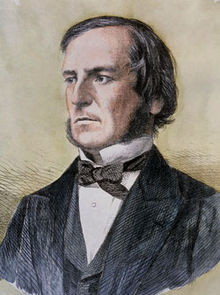
\includegraphics[width=0.9\columnwidth]{../img/boole}
\end{minipage}%
\begin{itemize}


\item Sammansatta logiska uttryck med logiska operatorer:\\
\code{&&} och, \texttt{||} eller, \texttt{!} icke, \code{==} likhet, \code{!=} olikhet,
relationer: \code{> < >= <=}

\item Exempel:
\begin{itemize}
\item[] \code{true && true}
\item[] \code{false || true}
\item[] \code{!false}
\item[] \code{42 == 43}
\item[] \code{42 != 43}
\item[] \code{(42 >= 43) || (1 + 1 == 2)}
\end{itemize}

\end{itemize}
\end{Slide}

\begin{Slide}{De Morgans lagar}

\href{https://en.wikipedia.org/wiki/Augustus_De_Morgan}{\Emph{De Morgans lagar}} beskriver vad som händer om man \Alert{negerar} ett logiskt uttryck. Kan användas för att göra \Emph{förenklingar}.

%$p$ och $q$ är logiska uttryck, $\neg$ står för ''icke'', $\wedge$ för ''och'', $\vee$ för ''eller'':
%\begin{eqnarray*}
%\neg (p \wedge q) & \Longleftrightarrow & (\neg p) \vee (\neg q)\\
%\neg (p \vee q) & \Longleftrightarrow & (\neg p) \wedge (\neg q)\\
%\end{eqnarray*}

\begin{itemize}
\item I all deluttryck sammanbundna med \code{&&} eller \code{||}, \\ ändra alla \code{&&} till \code{||} och omvänt.
\item Negera alla ingående deluttryck. En relation negeras genom att man byter \texttt{==} mot \texttt{!=}, \texttt{<} mot \texttt{>=}, etc.
\end{itemize}

Exempel på förenkling där de Morgans lagar används upprepat:

\begin{Code}[escapechar=X,backgroundcolor=,frame=none,basicstyle=\ttfamily\fontsize{10}{12}\selectfont]
! (a < b || (a == 1 && b == 1))             X$\iff$X
! (a < b) && ! (a == 1 && b == 1)           X$\iff$X
! (a < b) && (! (a == 1) || ! (b == 1))     X$\iff$X
a >= b && (a != 1 || b != 1)
\end{Code}
\end{Slide}

\begin{Slide}{Alternativ med if-uttryck}
\begin{itemize}
\item Ett if-uttryck börjar med nyckelordet \code{if}, följt av ett logiskt uttryck inom parentes och två grenar.
\begin{Code}
def slumpgrönsak = if (math.random() < 0.8) "gurka" else "tomat"
\end{Code}
\item Den ena grenen evalueras om uttrycket är \code{true}
\item Den andra \code{else}-grenen evalueras om uttrycket är \code{false}
\begin{REPLnonum}
scala> slumpgrönsak
res13: String = gurka

scala> slumpgrönsak
res14: String = gurka

scala> slumpgrönsak
res15: String = tomat

\end{REPLnonum}
\end{itemize}
\end{Slide}

\Subsection{Satser}


%%%%%%%%%%%%%%%%%%%%%%%%
\begin{Slide}{Variabeldeklaration och tilldelningssats}\SlideFontTiny

\begin{itemize}
\item En \Emph{variabeldeklaration} medför att \Alert{plats i datorns minne} reserveras så att värden av den typ som variabeln kan referera till får plats där.

\item Vid deklaration ska variabeln \Emph{initialiseras} med ett startvärde.

\item En \code{val}-deklaration ger en variabel som efter initialisering inte kan ändras.


\begin{multicols}{2}
Dessa deklarationer...
\begin{lstlisting}
var x = 42
val y = x + 1
\end{lstlisting}
... ger detta innehåll någonstans i minnet:

%http://tex.stackexchange.com/questions/18521/tikz-matrix-as-a-replacement-for-tabular
\begin{tikzpicture}[]
\matrix [matrix of nodes, row sep=0, column 2/.style={nodes={rectangle,draw,minimum width=3em}}]
{
x   & 42 \\
y   & 43 \\
};
\end{tikzpicture}
%\end{column}

%\end{columns}

\end{multicols}


\item Med en \Emph{tilldelningssats} ges en tidigare \code{var}-deklarerad variabel ett nytt värde:
\begin{lstlisting}
x = 13
\end{lstlisting}

\item Det gamla värdet försvinner för alltid och det nya värdet lagras istället: \\
\begin{tikzpicture}[]
\matrix [matrix of nodes, row sep=0, column 2/.style={nodes={rectangle,draw,minimum width=3em}}]
{
x   & 13 \\
y   & 43 \\
};
\end{tikzpicture}

Observera att \code{y} här inte påverkas av att x ändrade värde.
\end{itemize}
\end{Slide}

\begin{Slide}{Tilldelningssatser är \emph{inte} matematisk likhet}\SlideFontSmall

\begin{itemize}

\item Likhetstecknet används alltså för att \Emph{tilldela} variabler nya värden och det är \Alert{inte} samma sak som matematisk likhet. Vad händer här?
\begin{lstlisting}
x = x + 1
\end{lstlisting}

\item Denna syntax är ett arv från de gamla språken C, Fortran mfl.

\item I \href{https://en.wikipedia.org/wiki/Assignment_(computer_science)}{andra språk} används  t.ex.  \\\vspace{1em}
\texttt{x := x + 1}  \hspace{2em} eller  \hspace{2em} \texttt{x <- x + 1} \\\vspace{0.5em}

\item Denna syntax visar kanske bättre att tilldelning är en \Emph{stegvis process}:

\begin{enumerate}\SlideFontTiny
\item Först beräknas \Emph{uttrycket till höger} om tilldelningstecknet.
\item Sedan \Emph{ersätts värdet} som variabelnamnet refererar till av det beräknade uttrycket. Det gamla värdet \Alert{försvinner för alltid}.
\end{enumerate}

\end{itemize}

\end{Slide}


\begin{Slide}{Förkortade tilldelningssatser}
\begin{itemize}
\item Det är vanligt att man vill tilldela en variabel ett nytt värde som beror av det gamla, så som i \\\code{x = x + 1}

\item Därför finns \Emph{förkortade tilldelningssatser} som gör så att man sparar några tecken och det blir tydligare (?) vad som sker (när man vant sig vid detta skrivsätt):
\begin{Code}
x += 1
\end{Code}

\item Uttrycket ovan expanderas av kompilatorn till \code{x = x + 1}
\end{itemize}


\end{Slide}


\begin{Slide}{Exempel på förkortade tilldelningssatser}
\begin{REPLnonum}
scala> var x = 42
x: Int = 42

scala> x *= 2

scala> x
res0: Int = 84


scala> x /= 3

scala> x
res2: Int = 28
\end{REPLnonum}
\end{Slide}


\ifkompendium\else
\begin{Slide}{Övning: Tilldelningar i sekvens}\footnotesize

%\begin{columns}
%\begin{column}{0.32\textwidth}
\begin{minipage}{0.32\textwidth}

Rita hur minnet ser ut efter varje rad nedan:
\vskip1em
\begin{lstlisting}[ numbers=left,]
var u = 42
var x = 10
var y = 2 * x + 1
x = 20
var z = y + x + y - x
x += 1; y *= 2
\end{lstlisting}
%\end{column}
\end{minipage}\hspace{2em}%
%\begin{column}{0.6\textwidth}
\begin{minipage}{0.6\textwidth}


\scriptsize En variabel som ännu inte \Emph{initierats} har ett \Alert{odefinierat} värde, anges nedan med frågetecken.
\begin{table}[]
\centering\scriptsize
%http://tex.stackexchange.com/questions/83930/what-are-the-different-kinds-of-boxes-in-latex
\newcommand{\mybox}[1]{\raisebox{-0.5mm}{\framebox(21,14){#1}}\vspace{0.5mm}}
\begin{tabular}{@{}ccccccc}
 & rad 1 & rad 2 & rad 3 & rad 4  & rad 5 & rad 6\\
u& \mybox{42 } &  \mybox{}   &   \mybox{}   & \mybox{} & \mybox{} & \mybox{} \\
x& \mybox{? } &  \mybox{}   &   \mybox{}   & \mybox{} & \mybox{}  & \mybox{} \\
y& \mybox{? } &  \mybox{}   &   \mybox{}   & \mybox{} & \mybox{}  & \mybox{} \\
z& \mybox{? } &  \mybox{}   &   \mybox{}   & \mybox{} & \mybox{}  & \mybox{} \\
\end{tabular}
\end{table}

%\end{column}
%\end{columns}
\end{minipage}%
\end{Slide}
\fi



\begin{Slide}{Variabler som ändrar värden kan vara knepiga}
\begin{itemize}
\item Kod som innehåller variabler som \Alert{förändras} över tid är ofta svårare att läsa och begripa.

\item Många buggar beror på att variabler av misstag förändras på felaktiga och oanade sätt.

\item Föränderliga värden blir speciellt svåra i kod som körs jämlöpande (parallellt).

\item I kod som körs i skarpt läge med många användare (s.k. produktionskod) är därför \code{val} att föredra, medan \code{var} endast används om det \Alert{verkligen} behövs.
\item Alltså: räkna hellre ut nya värden än förändra befintliga.
\end{itemize}
\end{Slide}
%%%%%%%%%%



\begin{Slide}{Kontrollstrukturer: alternativ och repetition}\SlideFontSmall
Används för att kontrollera (förändra) sekvensen och skapa \Emph{alternativa} vägar genom koden. Vägen  bestäms vid körtid.
\begin{itemize}
\item if-sats:
\begin{Code}
if (math.random() < 0.8) println("gurka") else println("tomat")
\end{Code}
\end{itemize}

Olika sorters \Emph{loopar} för att repetera satser. Antalet repetitioner ges vid körtid.
\begin{itemize}
\item \code{while}-sats: bra när man \Alert{inte vet hur många gånger} det kan bli.
\begin{Code}
while (math.random() < 0.8) println("gurka")
\end{Code}

\item \code{for}-sats: bra när man \Alert{vill ange antalet repetitioner}:
\begin{Code}
for (i <- 1 to 10) println(s"gurka nr $i")
\end{Code}

\end{itemize}
\end{Slide}

%%%% GE mer detaljer eller överlåta till övning???
%\begin{Slide}{if-sats}
%\begin{itemize}
%\item
%\end{itemize}
%\end{Slide}
%
%\begin{Slide}{while-sats}
%\begin{itemize}
%\item
%\end{itemize}
%\end{Slide}
%
%\begin{Slide}{for-sats}
%\begin{itemize}
%\item
%\end{itemize}
%\end{Slide}

\begin{Slide}{Procedurer}\SlideFontSmall
\begin{itemize}
\item En \Emph{procedur} är en funktion som \Alert{gör} något intressant, men som \Alert{inte} lämnar något intressant returvärde.
\item Exempel på procedur i standardbiblioteket: \code{println("hej")}
\item Du \Emph{deklarerar egna procedurer} genom att ange \texttt{\Alert{Unit}} som returvärdestyp. Då returneras värdet \texttt{\Alert{()}} som betyder ''inget''.
\end{itemize}
\begin{REPLnonum}
scala> def hej(x: String): Unit = println(s"Hej på dej $x!")
hej: (x: String)Unit

scala> hej("Herr Gurka")
Hej på dej Herr Gurka!

scala> val x = hej("Fru Tomat")
Hej på dej Fru Tomat!
x: Unit = ()
\end{REPLnonum}
\begin{itemize}
\item Det som \Alert{görs} kallas (sido)\Emph{effekt}. Ovan är utskriften själva effekten.
\item Även funktioner kan ha sidoeffekter. De kallas då \Alert{oäkta} funktioner.
\end{itemize}
\end{Slide}

\begin{Slide}{Problemlösning: nedbrytning i abstraktioner som sen kombineras}\SlideFontSmall
\begin{itemize}
\item En av de allra viktigaste principerna inom programmering är \Emph{funktionell nedbrytning} där  \Emph{underprogram} i form av funktioner och procedurer skapas för att bli byggstenar som kombineras till mer avancerade funktioner och procedurer.

\item Genom de namn som definieras skapas \Emph{återanvändbara abstraktioner} som kapslar in det funktionen gör till ett ''byggblock''.

\item Bra ''byggblock'' gör det lättare att lösa svåra programmeringsproblem.

\item Abstraktioner som beräknar eller gör \Emph{en enda, väldefinierad sak} är enklare att använda, jämfört med de som gör många, helt olika saker.

\item Abstraktioner med \Emph{välgenomtänkta namn} är enklare att använda, jämfört med kryptiska eller missvisande namn.
\end{itemize}

\end{Slide}

\ifkompendium\else

\begin{SlideExtra}{Om veckans övning: \code{expressions}}\SlideFontSmall

\begin{itemize}
%!TEX encoding = UTF-8 Unicode

\item Förstå vad som händer när satser exekveras och uttryck evalueras.
\item Förstå sekvens, alternativ och repetition.
\item Känna till literalerna för enkla värden, deras typer och omfång.
\item Kunna deklarera och använda variabler och tilldelning, samt kunna rita bilder av minnessituationen då variablers värden förändras.
\item Förstå skillnaden mellan olika numeriska typer, kunna omvandla mellan dessa och vara medveten om noggrannhetsproblem som kan uppstå.
\item Förstå booleska uttryck och värdena \code{true} och \code{false}, samt kunna förenkla booleska uttryck.
\item Förstå skillnaden mellan heltalsdivision och flyttalsdivision, samt användning av rest vid heltalsdivision.
\item Förstå precedensregler och användning av parenteser i uttryck.
\item Kunna använda \code{if}-satser och \code{if}-uttryck.
\item Kunna använda \code{for}-satser och \code{while}-satser.
\item Kunna använda \code{math.random()} för att generera slumptal i olika intervaller.
\item Kunna beskriva skillnader och likheter mellan en procedur och en funktion.

\end{itemize}

\end{SlideExtra}

\begin{SlideExtra}{Om veckans labb: \code{kojo}}
\begin{itemize}
%!TEX encoding = UTF-8 Unicode

\item Kunna kombinera principerna sekvens, alternativ, repetition, och abstraktion i skapandet av egna program om minst 20 rader kod.
\item Kunna förklara vad ett program gör i termer av sekvens, alternativ, repetition, och abstraktion.
\item Kunna tillämpa principerna sekvens, alternativ, repetition, och abstraktion i enkla algoritmer.
\item Kunna formatera egna program så att de blir lätta att läsa och förstå.
\item Kunna förklara vad en variabel är och kunna skriva deklarationer och göra tilldelningar.
\item Kunna genomföra upprepade varv i cykeln \emph{editera-exekvera-felsöka/förbättra} för att successivt bygga upp allt mer utvecklade program.

\end{itemize}
\end{SlideExtra}

\fi

%%%%%%%%%%%%%%%%%%%%%%%%%%%%%%%%%%%%%% nedan redan meddelat i introveckan
%\ifkompendium\else
%\Subsection{Meddelande från \href{http://lth.se/code}{Code@LTH}}
%\fi









%\chapter{Introduktion}\label{chapter:W01}
\begin{itemize}[nosep]
\item sekvens
\item alternativ
\item repetition
\item abstraktion
\item programmeringsspråk
\item programmeringsparadigmer
\item editera-kompilera-exekvera
\item datorns delar
\item virtuell maskin
\item värde
\item uttryck
\item variabel
\item typ
\item tilldelning
\item namn
\item val
\item var
\item def
\item if
\item else
\item true
\item false
\item MinValue
\item MaxValue
\item aritmetik
\item slumptal
\item math.random
\item logiska uttryck
\item de Morgans lagar
\item while-sats
\item for-sats
\end{itemize}
%!TEX encoding = UTF-8 Unicode
%!TEX root = ../exercises.tex

\ifPreSolution
\Exercise{\ExeWeekONE}\label{exe:W01}

\begin{Goals}
%!TEX encoding = UTF-8 Unicode

\item Förstå vad som händer när satser exekveras och uttryck evalueras.
\item Förstå sekvens, alternativ och repetition.
\item Känna till literalerna för enkla värden, deras typer och omfång.
\item Kunna deklarera och använda variabler och tilldelning, samt kunna rita bilder av minnessituationen då variablers värden förändras.
\item Förstå skillnaden mellan olika numeriska typer, kunna omvandla mellan dessa och vara medveten om noggrannhetsproblem som kan uppstå.
\item Förstå booleska uttryck och värdena \code{true} och \code{false}, samt kunna förenkla booleska uttryck.
\item Förstå skillnaden mellan heltalsdivision och flyttalsdivision, samt användning av rest vid heltalsdivision.
\item Förstå precedensregler och användning av parenteser i uttryck.
\item Kunna använda \code{if}-satser och \code{if}-uttryck.
\item Kunna använda \code{for}-satser och \code{while}-satser.
\item Kunna använda \code{math.random()} för att generera slumptal i olika intervaller.
\item Kunna beskriva skillnader och likheter mellan en procedur och en funktion.

\end{Goals}

\begin{Preparations}
\item \StudyTheory{01}
\item Du behöver en dator med Scala och Kojo installerad, se appendix~\ref{appendix:compile} och  \ref{appendix:kojo}.
\end{Preparations}

\else

\ExerciseSolution{\ExeWeekONE}

\fi  %%% END \ifPreSolution


\BasicTasks




\WHAT{Para ihop begrepp med beskrivning.}

\QUESTBEGIN

\Task \what

\vspace{1em}\noindent Koppla varje begrepp med den (förenklade) beskrivning som passar bäst:

\begin{ConceptConnections}
  litteral & 1 & & A & kan inträffa medan programmet kör \\ 
  sträng & 2 & & B & att översätta kod till exekverbar form \\ 
  sats & 3 & & C & vid anrop beräknas ett returvärde \\ 
  uttryck & 4 & & D & decimaltal med begränsad noggrannhet \\ 
  funktion & 5 & & E & bra då antalet repetitioner är bestämt i förväg \\ 
  procedur & 6 & & F & en kodrad som gör något; kan särskiljas med semikolon \\ 
  exekveringsfel & 7 & & G & beskriver vad data kan användas till \\ 
  kompileringsfel & 8 & & H & antingen sann eller falsk \\ 
  abstrahera & 9 & & I & för att ändra en variabels värde \\ 
  kompilera & 10 & & J & kombinerar värden och funktioner till ett nytt värde \\ 
  typ & 11 & & K & en sekvens av tecken \\ 
  for-sats & 12 & & L & att införa nya begrepp som förenklar kodningen \\ 
  while-sats & 13 & & M & anger ett specifikt datavärde \\ 
  tilldelning & 14 & & N & kan inträffa innan exekveringen startat \\ 
  flyttal & 15 & & O & bra då antalet repetitioner ej är bestämt i förväg \\ 
  boolesk & 16 & & P & vid anrop sker (sido)effekt; returvärdet är tomt \\ 
\end{ConceptConnections}

\SOLUTION

\TaskSolved \what

\begin{ConceptConnections}
  litteral & 1 & ~~\Large$\leadsto$~~ &  D & anger ett specifikt datavärde \\ 
  sträng & 2 & ~~\Large$\leadsto$~~ &  G & en sekvens av tecken \\ 
  sats & 3 & ~~\Large$\leadsto$~~ &  F & en kodrad som gör något; kan särskiljas med semikolon \\ 
  uttryck & 4 & ~~\Large$\leadsto$~~ &  H & kombinerar värden och funktioner till ett nytt värde \\ 
  funktion & 5 & ~~\Large$\leadsto$~~ &  K & vid anrop beräknas ett returvärde \\ 
  procedur & 6 & ~~\Large$\leadsto$~~ &  J & vid anrop sker (sido)effekt; returvärdet är tomt \\ 
  exekveringsfel & 7 & ~~\Large$\leadsto$~~ &  N & kan inträffa medan programmet kör \\ 
  kompileringsfel & 8 & ~~\Large$\leadsto$~~ &  M & kan inträffa innan exekveringen startat \\ 
  abstrahera & 9 & ~~\Large$\leadsto$~~ &  A & att införa nya begrepp som förenklar kodningen \\ 
  kompilera & 10 & ~~\Large$\leadsto$~~ &  C & att översätta kod till exekverbar form \\ 
  typ & 11 & ~~\Large$\leadsto$~~ &  I & beskriver vad data kan användas till \\ 
  for-sats & 12 & ~~\Large$\leadsto$~~ &  O & bra då antalet repetitioner är bestämt i förväg \\ 
  while-sats & 13 & ~~\Large$\leadsto$~~ &  P & bra då antalet repetitioner ej är bestämt i förväg \\ 
  tilldelning & 14 & ~~\Large$\leadsto$~~ &  L & för att ändra en variabels värde \\ 
  flyttal & 15 & ~~\Large$\leadsto$~~ &  E & decimaltal med begränsad noggrannhet \\ 
  boolesk & 16 & ~~\Large$\leadsto$~~ &  B & antingen sann eller falsk \\ 
\end{ConceptConnections}

\QUESTEND






\WHAT{Utskrift i Scala REPL.}

\QUESTBEGIN

\Task \what

\vspace{1em}\noindent Starta Scala REPL \Eng{Read-Evaluate-Print-Loop}.

\begin{REPLnonum}
> scala
Welcome to Scala 3.0.1 (OpenJDK 64-Bit Server VM, Java 11.0.8).
Type in expressions for evaluation. Or try :help.
scala -version.
scala>
\end{REPLnonum}

\Subtask Skriv efter prompten \code{scala>} en sats som skriver ut en valfri (bruklig/knasig) hälsningsfras, genom anrop av proceduren \code{println} med något strängargument. Tryck på \textit{Enter} så att satsen kompileras och exekveras.

\Subtask Skriv samma sats igen (eller tryck pil-upp) men ''glöm bort'' att skriva högerparentesen efter argumentet innan du trycker på \textit{Enter}. Vad händer?

\begin{framed}
\noindent\emph{Tips inför fortsättningen:} Det finns många användbara kortkommandon och andra trix för att jobba snabbt i REPL. Be gärna någon som kan dessa trix att visa dig hur man kan jobba snabbare. Läs appendix \ref{appendix:compile:REPL} och prova sedan att kopiera och klistra in text. Använd piltangenterna för att bläddra i historiken, Ctrl+A för att komma till början av raden, Ctrl+K för att radera resten av raden, etc.
\end{framed}



\SOLUTION
\TaskSolved \what

\SubtaskSolved Till exempel:
\begin{REPLnonum}
scala> println("hejsan svejsan")
\end{REPLnonum}

\SubtaskSolved Om högerparentes fattas får man fortsätta skriva på nästa rad. Detta indikeras med vertikalstreck i början av varje ny rad:
\begin{REPLnonum}
scala> println("hejsan svejsan"
     | + "!"
     | )
hejsan svejsan!
\end{REPLnonum}

\QUESTEND



\WHAT{Konkatenering av strängar.}

\QUESTBEGIN

\Task \what

\Subtask Skriv ett uttryck som konkatenerar två strängar, t.ex. \code{"gurk"} och \code{"burk"}, med hjälp av operatorn \code{+} och studera resultatet. Vad har uttrycket för värde och typ? Vilken siffra står efter ordet \code{res} i variabeln som lagrar resultatet?

\Subtask Använd resultatet från konkateneringen, t.ex. \code{res0} (byt ev. ut \code{0}:an mot siffran efter \code{res} i utskriften från förra evalueringen), och skriv ett uttryck med hjälp av operatorn \code{*} som upprepar resultatet från förra deluppgiften 42 gånger.


\SOLUTION

\TaskSolved \what

\SubtaskSolved
\begin{REPLnonum}
scala> "gurk" + "burk"
res1: String = gurkburk
\end{REPLnonum}
värde: \code{"gurkburk"}, typ:  \code{String}

\SubtaskSolved
\begin{REPLnonum}
scala> res1 * 42
res2: String = gurkatomatgurkatomatgurkatomatgurkatomatgurkatomatgurkatomatgurkatomatgurkatomatgurkatomatgurkatomatgurkatomatgurkatomatgurkatomatgurkatomatgurkatomatgurkatomatgurkatomatgurkatomatgurkatomatgurkatomatgurkatomatgurkatomatgurkatomatgurkatomatgurkatomatgurkatomatgurkatomatgurkatomatgurkatomatgurkatomatgurkatomatgurkatomatgurkatomatgurkatomatgurkatomatgurkatomatgurkatomatgurkatomatgurkatomatgurkatomatgurkatomatgurkatomat
\end{REPLnonum}

\QUESTEND




\WHAT{När upptäcks felet?}

\QUESTBEGIN

\Task \what

\Subtask Vad har uttrycket \code{ "hej" * 3 } för typ och värde? Testa i REPL.

\Subtask Byt ut 3:an ovan mot ett så pass stort heltal så att minnet blir fullt. Hur börjar felmeddelandet? Är detta ett körtidsfel eller ett kompileringsfel?

\Subtask Välj ett värde på argumentet efter operatorn \code{*} så att ett typfel genereras. Hur börjar felmeddelandet? Är detta ett körtidsfel eller ett kompileringsfel?

\begin{framed}
\noindent\emph{Tips inför fortsättningen:} Gör gärna fel när du kodar så lär du dig mer! Träna på att tolka olika felmeddelanden och fråga någon om hjälp om du inte förstår. Kompilatorns utskrifter kan vara till stor hjälp, men är ibland kryptiska. Om du kör fast och inte kommer vidare själv så be om hjälp, \emph{men be om tips snarare än färdiga lösningar} så att du behåller initiativet själv och tar kontroll över nästa steg i ditt lärande.
\end{framed}


\SOLUTION

\TaskSolved \what

\SubtaskSolved Typ: \code{String}, värde: \code{"hejhejhej"}

\SubtaskSolved Körtiddsfel:
\begin{REPLnonum}
scala> "hej" * Int.MaxValue
java.lang.OutOfMemoryError: Java heap space
\end{REPLnonum}

\SubtaskSolved Kompileringsfel: (indikeras av texten \code{<console> ... error:})
\begin{REPLnonum}
scala> "hej" * true
<console>:12: error: type mismatch;
 found   : Boolean(true)
 required: Int
       "hej" * true
\end{REPLnonum}
Ett typfel innebär att kompilatorn inte kan få typerna att överensstämma i t.ex. ett funktionsanrop. I Scala får vi reda på typfel redan vid kompilering medan i andra språk (t.ex. Javascript) upptäcks sådana fel under exekveringen, i värsta fall genom svårhittade buggar som kanske först märks långt senare.

\QUESTEND




\WHAT{Litteraler och typer.}

\QUESTBEGIN

\Task \what

\Subtask Ta hjälp av REPL-kommadot \verb+:type+ (kan förkortas \code{:t}) vid behov för att para ihop nedan litteraler med rätt typ.

\begin{ConceptConnections}[0.35\textwidth]
  \code|1    | & 1 & & A & \code|Float  | \\ 
  \code|1L   | & 2 & & B & \code|Double | \\ 
  \code|1.0  | & 3 & & C & \code|Unit   | \\ 
  \code|1D   | & 4 & & D & \code|Int    | \\ 
  \code|1F   | & 5 & & E & \code|Boolean| \\ 
  \code|'1'  | & 6 & & F & \code|Long   | \\ 
  \code|"1"| & 7 & & G & \code|String | \\ 
  \code|true | & 8 & & H & \code|Double | \\ 
  \code|false| & 9 & & I & \code|Char   | \\ 
  \code|()   | & 10 & & J & \code|Boolean| \\ 
%\Connect{\code|1      |}  {\code|Int    |}
%\Connect{\code|1L     |}  {\code|Long   |}
%\Connect{\code|1.0    |}  {\code|Double |}
%\Connect{\code|1D     |}  {\code|Double |}
%\Connect{\code|1F     |}  {\code|Float  |}
%\Connect{\code|'1'    |}  {\code|Char   |}
%\Connect{\code|\"1\"  |}  {\code|String |}
%\Connect{\code|true   |}  {\code|Boolean|}
%\Connect{\code|false  |}  {\code|Boolean|}
%\Connect{\code|()     |}  {\code|Unit   |}
\end{ConceptConnections}

\Subtask Vad händer om du adderar 1 till det största möjliga värdet av typen \code{Int}?
\\\emph{Tips:} se snabbreferensen \footnote{\url{http://cs.lth.se/pgk/quickref/}} under rubriken ''The Scala type system'' avsnitt ''Methods on numbers''.

\Subtask Vad är skillnaden mellan typerna \code{Long} och \code{Int}?

\Subtask Vad är skillnaden mellan typerna \code{Double} och \code{Float}?


\SOLUTION

\TaskSolved \what

\SubtaskSolved

\begin{ConceptConnections}
  \code|1    | & 1 & ~~\Large$\leadsto$~~ &  C & \code|Int    | \\ 
  \code|1L   | & 2 & ~~\Large$\leadsto$~~ &  F & \code|Long   | \\ 
  \code|1.0  | & 3 & ~~\Large$\leadsto$~~ &  J & \code|Double | \\ 
  \code|1D   | & 4 & ~~\Large$\leadsto$~~ &  D & \code|Double | \\ 
  \code|1F   | & 5 & ~~\Large$\leadsto$~~ &  B & \code|Float  | \\ 
  \code|'1'  | & 6 & ~~\Large$\leadsto$~~ &  A & \code|Char   | \\ 
  \code|"1"| & 7 & ~~\Large$\leadsto$~~ &  E & \code|String | \\ 
  \code|true | & 8 & ~~\Large$\leadsto$~~ &  G & \code|Boolean| \\ 
  \code|false| & 9 & ~~\Large$\leadsto$~~ &  I & \code|Boolean| \\ 
  \code|()   | & 10 & ~~\Large$\leadsto$~~ &  H & \code|Unit   | \\ 
%\ConnectSolved{\code|1      |}  {\code|Int    |}
%\ConnectSolved{\code|1L     |}  {\code|Long   |}
%\ConnectSolved{\code|1.0    |}  {\code|Double |}
%\ConnectSolved{\code|1D     |}  {\code|Double |}
%\ConnectSolved{\code|1F     |}  {\code|Float  |}
%\ConnectSolved{\code|'1'    |}  {\code|Char   |}
%\ConnectSolved{\code|\"1\"  |}  {\code|String |}
%\ConnectSolved{\code|true   |}  {\code|Boolean|}
%\ConnectSolved{\code|false  |}  {\code|Boolean|}
\end{ConceptConnections}

\SubtaskSolved Värdet går över gränsen för vad som får plats i ett 32 bitars heltal och ''börjar om'' på det minsta möjliga heltalet \code{Int.MinValue} eftersom det är så binär aritmetik aritmetik med begränsat antal bitar fungerar i CPU:n.
\begin{REPL}
scala> Int.MaxValue + 1
res3: Int = -2147483648

scala> Int.MinValue
res4: Int = -2147483648
\end{REPL}

\SubtaskSolved Båda är heltal men \code{Long} kan representera större tal än \code{Int}.

\SubtaskSolved Båda är flyttal men \code{Double} har dubbel precision och kan representera större tal med fler decimaler.



\QUESTEND





\WHAT{Matematiska funktioner. Scaladoc.}

\QUESTBEGIN

\Task \what

\Subtask Antag att du har ett schackbräde med 64 rutor. Tänk dig att du börjar med att lägga ett enda riskorn på första rutan och sedan 
lägger dubbelt så många riskorn i en ny hög för varje efterföljande ruta: 1, 2, 4, 8, ...  etc. När du har gjort detta för alla rutor, 
hur många riskorn har du totalt lagt på schackbrädet?\footnote{\url{https://en.wikipedia.org/wiki/Wheat_and_chessboard_problem}}

\emph{Tips:} Du ska beräkna $2^{64} - 1$. Om du skriver \code{math.} i REPL och trycker TAB får du se inbyggda matematiska funktioner i Scalas standardbibliotek:
\begin{REPLnonum}
scala> math.    // Tryck TAB direkt efter punkten och betrakta listan
\end{REPLnonum}
Använd funktionen \code{math.pow} och lämpliga argument. Om du anger \code{math.pow} eller \code{math.pow()} utan argument får du se funktionshuvudet med 
parameterlistan.

Om du surfar till \url{http://www.scala-lang.org/api/current/} och skriver \code{math} i sökrutan och sedan, efter att du klickat på 
\textbf{\texttt{\small scala.math}}, skriver \textbf{\texttt{\small pow}} i rutan längre ner, så filtreras sidan och du hittar dokumentationen 
av \code{ def pow } som du kan klicka på och läsa mer om.

\Subtask Definiera funktionen \code{omkrets} nedan i REPL. Går det bra att utelämna returtyp-annoteringen? Varför? Finns det anledning att ha den kvar?
\begin{Code}
def omkrets(radie: Double): Double = 2 * math.Pi * radie
\end{Code}

\Subtask Jordens (genomsnittliga) diameter (vid ekvatorn) är ca $12 750$ $km$. Skriv ett uttryck som anropar funktionen \code{omkrets} ovan för att beräkna hur många kilometer per dag man ungefär måste färdas om man vill åka jorden runt på 80 dagar.

\SOLUTION

\TaskSolved \what

\SubtaskSolved Beräkning av $2^{64} - 1$ med \code{math.pow} enligt nedan ger ungefär $1.8 \cdot 10^{19}$
\begin{REPL}
scala> math.pow(2, 64) - 1
res0: Double = 1.8446744073709552E19
\end{REPL}

\SubtaskSolved Ja, returtyp-annoteringen \code{: Double} kan utelämnas.

\begin{itemize}
\item Varför kan returtyp utelämnas?\\Eftersom kompilatorns typhärledning kan härleda returtypen.
\item Varför kan man vilja utelämna den?\\Det blir kortare att skriva utan.
\item Anledningar att ange returtyp:
\begin{itemize}
\item  Med explicit returtyp får du hjälp av kompilatorn att redan under kompileringen kontrollera att uttrycket till höger om likhetstecknet har den typ som förväntas.

\item Genom att du anger returtypen explicit får de som enbart läser metodhuvudet (och inte implementationen)
 tydligt se vad som returneras.
\end{itemize}
\end{itemize}

\SubtaskSolved Ca $500$ $km$.
\begin{REPL}
scala> omkrets(12750 / 2) / 80
res0: Double = 500.6913291658733
\end{REPL}

\QUESTEND




\WHAT{Variabler och tilldelning. Förändringsbar och oföränderlig variabel.}

\QUESTBEGIN

\Task \what~

\Subtask Rita en \emph{ny} bild av datorns minne efter \emph{varje} exekverad rad 1--6 nedan. Varje bild ska visa alla variabler som finns i minnet och deras variabelnamn, typ och värde.

\begin{REPL}[numbers=left, numberstyle=\color{black}\ttfamily\scriptsize\selectfont]
scala> var a = 13
scala> val b = a + 1
scala> var c = (a + b) * 2.0
scala> b = 0
scala> a = 0
scala> c = c + 1
\end{REPL}
Efter första raden ser minnessituationen ut så här:

\MEM{a}{Int}{13}

\Subtask Varför blir det fel på rad 4? Är det ett kompileringsfel eller exekveringsfel? Hur lyder felmeddelandet?

\SOLUTION

\TaskSolved \what

\SubtaskSolved

\begin{tabular}{@{}l l l}
\MEM{{\it Efter rad 1:~~~~} a}{Int}{13}\\
\MEM{{\it Efter rad 2:~~~~} a}{Int}{13} & \MEM{b}{Int}{14}\\
\MEM{{\it Efter rad 3:~~~~} a}{Int}{13} & \MEM{b}{Int}{14} & \MEM{c}{Double}{54.0}\\
\MEM{{\it Efter rad 4:~~~~} a}{Int}{13} & \MEM{b}{Int}{14} & \MEM{c}{Double}{54.0}\\
\MEM{{\it Efter rad 5:~~~~} a}{Int}{0} & \MEM{b}{Int}{14} & \MEM{c}{Double}{54.0}\\
\MEM{{\it Efter rad 6:~~~~} a}{Int}{0} & \MEM{b}{Int}{14} & \MEM{c}{Double}{55.0}\\
\end{tabular}

\SubtaskSolved
Oföränderliga variabler deklareras med nyckelordet \code{val}. Det går inte att tilldela en oföränderlig variabel ett nytt värde; vid försök blir det kompileringsfel som lyder \texttt{\textbf{error: reassignment to val}}. Kompileringsfel känns igen med hjälp av texten \texttt{\textbf{error:}}, så som visas nedan:
\begin{REPLnonum}
scala> b = 0
<console>:12: error: reassignment to val
       b = 0
         ^
\end{REPLnonum}

\QUESTEND


\WHAT{Slumptal med \code{math.random()}.}

\QUESTBEGIN

\Task\label{exercise:expressions:roll} \what

\Subtask Vad ger funktionen \code{math.random()} för resultatvärde? Vilken typ? Vad är största och minsta möjliga värde?
\\\emph{Tips:} Se scaladoc här: \Scaladoc och prova i REPL.

\Subtask Deklarera den parameterlösa funktionen \code{def roll: Int = ???} som ska representera ett tärningskast och ge ett slumpmässigt heltal mellan 1 och 6. Testa funktionen genom att anropa den många gånger. \\\emph{Tips:} Använd \code{math.random()} och multiplicera och addera med lämpliga heltal. Omge beräkningen med parenteser och avsluta med \code{.toInt} för att avkorta decimaler och omvandla typen från \code{Double} till \code{Int}.

\SOLUTION

\TaskSolved \what

\SubtaskSolved Ur dokumentationen:
\begin{Code}
/** Returns a Double value with a positive sign,
 *  greater than or equal to 0.0 and less than 1.0.
 */
def random(): Double
\end{Code}
Dokumentationskommentarer, som börjar med \code{/**} och slutar med \code{*/}, ger oss en beskrivning av hur funktionen fungerar. Efter dokumentationskommentaren kommer funktionshuvudet, som här berättar att funktionen heter \code{random} och alltid kommer att returnera en \code{Double}. (Verktyget \code{scaladoc} kan med hjälp av  dokumentationskommentarerna automatiskt generera webbsajter med speciella  dokumentationssidor och sökfunktioner.)

\SubtaskSolved
\begin{REPL}
scala> def roll: Int = (math.random() * 6 + 1).toInt

scala> roll
res0: Int = 4

scala> roll
res1: Int = 1
\end{REPL}

\QUESTEND




\WHAT{Repetition med \code{for}, \code{foreach} och \code{while}.}

\QUESTBEGIN

\Task \what

\Subtask Så här kan en \code{for}-sats ser ut:
\begin{Code}
for i <- 1 to 10 do print(s"$i, ")
\end{Code}
Använd en \code{for}-sats för att skriva ut resultatet av 100 tärningskast med funktionen \code{roll} från uppgift \ref{exercise:expressions:roll}.

\Subtask Så här kan en \code{foreach}-sats ser ut:
\begin{Code}
(1 to 10).foreach(i => print(s"$i, "))
\end{Code}
Använd en \code{foreach}-sats för att skriva ut resultatet av 100 tärningskast med funktionen \code{roll} från uppgift \ref{exercise:expressions:roll}.

\Subtask Så här kan en \code{while}-sats se ut:
\begin{Code}
var i = 1
while i <= 10 do { print(s"$i, "); i = i + 1 }
\end{Code}
Använd en \code{while}-sats för att skriva ut resultatet av 100 tärningskast med funktionen \code{roll} från uppgift \ref{exercise:expressions:roll}. Vad händer om du glömmer \code{i = i + 1} ?


\SOLUTION

\TaskSolved \what

\SubtaskSolved
\begin{Code}
for i <- 1 to 100 do print(s"$roll, ")
\end{Code}

\SubtaskSolved
\begin{Code}
(1 to 100).foreach(i => print(s"$roll, "))
\end{Code}


\SubtaskSolved
\begin{Code}
var i = 1
while i <= 100 do { print(s"$roll, "); i = i + 1 }
\end{Code}

\begin{Code}
var i = 1
while i <= 100 do
    print(s"$roll, ") 
    i += 1
\end{Code}




\QUESTEND






\WHAT{Alternativ med \code{if}-sats och \code{if}-uttryck.}

\QUESTBEGIN

\Task \what

\Subtask Så här kan en \code{if}-sats se ut (notera dubbla likhetstecken):
\begin{Code}
if roll == 3 then println("TRE") else println("INTE TRE")
\end{Code}
Testa ovan i REPL. Skriv sedan en \code{for}-sats som kastar 100 tärningar och skriver ut strängen \code{"GRATTIS! "} om det blir en sexa, annars en ledsen smiley: \code{":("}

\Subtask Så här kan ett \code{if}-uttryck se ut:
\begin{Code}
if roll < 6 then 0 else 1
\end{Code}
Testa ovan i REPL. Skriv sedan en \code{while}-sats som kastar 100 tärningar och räknar antalet sexor. Skriv ut antalet efter \code{while}-satsen.

\SOLUTION

\TaskSolved \what

\SubtaskSolved
\begin{Code}
for i <- 1 to 100 do 
  if roll == 6 then print("GRATTIS! ") else print(":(")
\end{Code}
eller
\begin{Code}
for (i <- 1 to 100) if (roll == 6) print("GRATTIS! ") else print(":(")
\end{Code}

\SubtaskSolved
\begin{Code}
var i = 1
var n = 0
while i <= 100 do
  if roll == 6 then n = n + 1
  i = i + 1
println("Antalet sexor: " + n)
\end{Code}


\QUESTEND



\WHAT{Sekvens, sats och block.}

\QUESTBEGIN

\Task \what

\Subtask Vad gör dessa satser?
\begin{REPLnonum}
scala> def p = { print("san"); print("!"); println("hej")}
scala> p;p;p;p
\end{REPLnonum}

\Subtask
Använd pil-upp för att få tillbaka raden du skrev med definitionen av proceduren \code{p}. Byt plats på strängarna i utskriftsanropen i proceduren \code{p} så att utskriften blir:
\begin{REPLnonum}
hejsan!
hejsan!
hejsan!
hejsan!
\end{REPLnonum}

\Subtask Hur tolkar kompilatorn klammerparenteser och semikolon? Vad är ett block?

\SOLUTION

\TaskSolved \what

\SubtaskSolved
Satserna skapar denna utskrift:
\begin{REPLnonum}
san!hej
san!hej
san!hej
san!hej
\end{REPLnonum}

\SubtaskSolved
\begin{REPLnonum}
scala> def p = { print("hej"); print("san"); println("!")}
scala> p;p;p;p
\end{REPLnonum}

\SubtaskSolved
\begin{itemize}
\item Klammerparenteser används för att gruppera flera satser. 
Klammerparenteser behövs om man vill definiera en funktion som består av mer än en sats. 
Sedan scala 3 kan man istället använda indentering för att definera en funktion med flera rader och satser.

\item Semikolon särskiljer flera satser. Semikolon behövs om man vill skriva många satser på samma rad.


\end{itemize}

\QUESTEND




\WHAT{Heltalsdivision.}

\QUESTBEGIN

\Task \what~Vilket värde och vilken typ hör till vilket uttryck?  Är du osäker på svaret, testa i REPL.

\begin{ConceptConnections}[0.3\textwidth]
  \code| 4 / 42      | & 1 & & A & \code|    4: Int      | \\ 
  \code| 42.0 / 2    | & 2 & & B & \code|   10: Int      | \\ 
  \code| 42 / 4      | & 3 & & C & \code| 21.0: Double   | \\ 
  \code| 42 % 4      | & 4 & & D & \code|true : Boolean  | \\ 
  \code| 4 % 42      | & 5 & & E & \code|false: Boolean  | \\ 
  \code| 40 % 4 == 0 | & 6 & & F & \code|    0: Int      | \\ 
  \code| 42 % 4 == 0 | & 7 & & G & \code|    2: Int      | \\ 
\end{ConceptConnections}

\SOLUTION

\TaskSolved \what

\begin{ConceptConnections}[0.3\textwidth]
  \code| 4 / 42      | & 1 & ~~\Large$\leadsto$~~ &  D & \code|    0: Int      | \\ 
  \code| 42.0 / 2    | & 2 & ~~\Large$\leadsto$~~ &  A & \code| 10.5: Double   | \\ 
  \code| 42 / 4      | & 3 & ~~\Large$\leadsto$~~ &  C & \code|   10: Int      | \\ 
  \code| 42 % 4      | & 4 & ~~\Large$\leadsto$~~ &  E & \code|    2: Int      | \\ 
  \code| 4 % 42      | & 5 & ~~\Large$\leadsto$~~ &  B & \code|    4: Int      | \\ 
  \code| 40 % 4 == 0 | & 6 & ~~\Large$\leadsto$~~ &  G & \code|true : Boolean  | \\ 
  \code| 42 % 4 == 0 | & 7 & ~~\Large$\leadsto$~~ &  F & \code|false: Boolean  | \\ 
\end{ConceptConnections}

\QUESTEND





\WHAT{Booleska värden.}

\QUESTBEGIN

\Task \what~Vilket värde har dessa uttryck?  % Uppgift 13

\Subtask \code{true && true}

\Subtask \code{false && true}

\Subtask \code{true || true}

\Subtask \code{false || true}


\Subtask \code{false || false}

\Subtask \code{true == true}

\Subtask \code{true != false}


\Subtask \code{true > false}

\Subtask \code{true && (1 / 0 > 1)}

\Subtask \code{false && (1 / 0 > 1)}

\SOLUTION

\TaskSolved \what

\SubtaskSolved \code{true}

\SubtaskSolved \code{false}

\SubtaskSolved \code{true}

\SubtaskSolved \code{true}


\SubtaskSolved \code{false}

\SubtaskSolved \code{true}

\SubtaskSolved \code{true}


\SubtaskSolved \code{true}

\SubtaskSolved Undantag kastas: \code{java.lang.ArithmeticException: / by zero}

\SubtaskSolved \code{false}

\QUESTEND





\WHAT{Booleska variabler.}

\QUESTBEGIN

\Task \what~Vad skrivs ut på rad 2 och 4 nedan?

\begin{REPL}
scala> var monster = false
scala> if monster then println("akta dig!!!")
scala> monster = true
scala> if monster then println("akta dig!!!")
\end{REPL}

\SOLUTION

\TaskSolved \what

\begin{itemize}
\item[2:] Ingenting skrivs ut.
\item[4:] \code{akta dig!!!}
\end{itemize}


\QUESTEND






\WHAT{Turtle graphics med Kojo.}

\QUESTBEGIN

\Task \what~På veckans laboration ska du använda Kojo för att verifiera att du kan använda sekvens, alternativ, repetition och abstraktion. Med Kojo ska du skapa Scala-program som ritar färgglada figurer med hjälp av ett lättanvänt Scala-bibliotek för \emph{turtle graphics}\footnote{\url{https://en.wikipedia.org/wiki/Turtle_graphics}}.

Starta Kojo (se appendix \ref{appendix:kojo}). Om du inte redan har svenska menyer: välj svenska i språkmenyn och starta om Kojo.  Skriv in nedan program och tryck på den \emph{gröna} play-knappen. Notera kopplingen mellan satssekvensen och vad som händer i ritfönstret.

\begin{Code}
sudda

fram; höger
fram; vänster
färg(grön)
fram
\end{Code}
\noindent


\Subtask Vad händer om du \emph{inte} börjar programmet med \code{sudda} och kör samma program upprepade gånger? Varför är det bra att börja programmet med \code{sudda}?

\Subtask Skriv kod som ritar en kvadrat enligt bilden nedan.
\vspace{1em}\\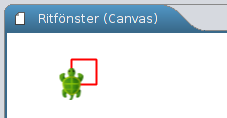
\includegraphics[width=0.47\textwidth]{../img/kojo/kvadrat}

\noindent Prova gärna olika sätt att skriva din kod \emph{utan} att resultatet ändras: skriv satser i sekvens på flera rader eller satser i sekvens på samma rad med semikolon emellan; använd blanktecken och blanka rader i koden. Hur vill du gruppera dina satser så att de är lätta för en människa att läsa?
%Prova att ändra på \emph{ordningen} mellan satserna och studera hur resultatet påverkas. Använd den \emph{gula} play-knappen  (programspårning) för att studera exekveringen i detalj. Vad händer du klickar på satser i ditt program och på rutor i programspårningen?


\Subtask Rita en trappa enligt bilden nedan.


\includegraphics[width=0.3\textwidth]{../img/kojo/stairs}

\Subtask Rita valfri bild på valfri bakgrund med hjälp av några av procedurerna i tabellen nedan. Du kan till exempel rita en rosa triangel med lila konturer mot svart bakgrund. % \ref{lab:kojo:kojo-procedures}.
Försök att underlätta läsbarheten av din kod med hjälp av lämpliga radbrytningar och gruppering av satser.


\begin{table}[H]
\begin{longtable}{l l}\small
\code|fram(100)| & Paddan går framåt 100 steg (25 om argument saknas).\\
\code|färg(rosa)| & Sätter pennans färg till rosa. \\
\code|fyll(lila)| & Sätter ifyllnadsfärgen till lila. \\
\code|fyll(genomskinlig)| & Gör så att paddan \emph{inte} fyller i något när den ritar. \\
\code|bredd(20)| & Gör så att pennan får bredden 20. \\
\code|bakgrund(svart)| & Bakgrundsfärgen blir svart. \\
\code|bakgrund2(grön,gul)| & Bakgrund med övergång från grönt till gult. \\
\code|pennaNer|  & Sätter ner paddans penna så att den ritar när den går. \\
\code|pennaUpp|  & Sänker paddans penna så att den \emph{inte} ritar när den går. \\
\code|höger(45)|   & Paddan vrider sig 45 grader åt höger. \\
\code|vänster(45)| & Paddan vrider sig 45 grader åt vänster. \\
\code|hoppa|       & Paddan hoppar 25 steg utan att rita. \\
\code|hoppa(100)|  & Paddan hoppar 100 steg utan att rita. \\
\code|hoppaTill(100, 200)| & Paddan hoppar till läget (100, 200) utan att rita. \\
\code|gåTill(100, 200)|    & Paddan vrider sig och går till läget (100, 200). \\
\code|öster|   & Paddan vrider sig så att nosen pekar åt höger. \\
\code|väster|  & Paddan vrider sig så att nosen pekar åt vänster. \\
\code|norr|    & Paddan vrider sig så att nosen pekar uppåt. \\
\code|söder|   & Paddan vrider sig så att nosen pekar neråt. \\
\code|mot(100,200)|   & Paddan vrider sig så att nosen pekar mot läget (100, 200) \\
\code|sättVinkel(90)| & Paddan vrider nosen till vinkeln 90 grader. \\
\end{longtable}
%\label{lab:kojo:kojo-procedures}
%\caption{Några användbara procedurer i Kojo.}
\end{table}

\begin{framed}
\noindent\emph{Tips inför fortsättningen:} Ha gärna både REPL och Kojo igång samtidigt. Då kan du undersöka hur olika kodkonstruktioner fungerar i REPL, medan du stegvis skapar allt större program i editorn i Kojo. Detta sätt att jobba har du nytta av under resten av kursen, både om du använder en texteditor och kompilerar i terminalen, och om du använder en professionell integrerad utvecklingsmiljö. Oavsett vilka andra verktyg du kör är det användbart att ha REPL igång i ett eget fönster som hjälp i den kreativa processen, medan du jagar buggar och medan du lär dig nya koncept. Så fort du undrar hur något fungerar i Scala: fram med REPL och testa!
\end{framed}


\SOLUTION

\TaskSolved \what

\SubtaskSolved Genom att börja din Kojo-program med \code{sudda} så startar du exekveringen i samma utgångsläge: en tom rityta \Eng{canvas} där paddan pekar uppåt, pennan är nere och pennans färg är röd.  Då blir det lättare att resonera om vad programmet gör från början till slut, jämfört med om exekveringen beror på resultatet av tidigare exekveringar.


\SubtaskSolved
\begin{Code}
sudda

fram; vänster
fram; vänster
fram; vänster
fram; vänster
\end{Code}


\SubtaskSolved
\begin{Code}
sudda

fram; vänster
fram; höger

fram; vänster
fram; höger

fram; vänster
fram; höger

fram; vänster
\end{Code}


\QUESTEND









\clearpage

\ExtraTasks %%%%%%%%%%%%%%%%%% EXTRAUPPGIFTER



\WHAT{Typ och värde.}

\QUESTBEGIN

\Task \what~Vilket värde och vilken typ hör till vilket uttryck?  Är du osäker på svaret, testa i REPL.

\begin{ConceptConnections}[0.3\textwidth]
  \code|1.0 + 18          | & 1 & & A & \code|42.0: Double    | \\ 
  \code|(41 + 1).toDouble | & 2 & & B & \code|65: Int         | \\ 
  \code|1.042e42 + 1      | & 3 & & C & \code|19.0: Double    | \\ 
  \code|12E6.toLong       | & 4 & & D & \code|12000000: Long  | \\ 
  \code|32.toChar.toString| & 5 & & E & \code|'*': Char       | \\ 
  \code|'A'.toInt         | & 6 & & F & \code|48: Int         | \\ 
  \code|0.toInt           | & 7 & & G & \code|" ": String   | \\ 
  \code|'0'.toInt         | & 8 & & H & \code|1.042E42: Double| \\ 
  \code|'9'.toInt         | & 9 & & I & \code|'q': Char       | \\ 
  \code|'A' + '0'         | & 10 & & J & \code|113: Int        | \\ 
  \code|('A' + '0').toChar| & 11 & & K & \code|0: Int          | \\ 
  \code|"*!%#".charAt(0)| & 12 & & L & \code|57: Int         | \\ 
\end{ConceptConnections}

\SOLUTION

\TaskSolved \what

\begin{ConceptConnections}
  \code|1.0 + 18          | & 1 & ~~\Large$\leadsto$~~ &  E & \code|19.0: Double    | \\ 
  \code|(41 + 1).toDouble | & 2 & ~~\Large$\leadsto$~~ &  L & \code|42.0: Double    | \\ 
  \code|1.042e42 + 1      | & 3 & ~~\Large$\leadsto$~~ &  A & \code|1.042E42: Double| \\ 
  \code|12E6.toLong       | & 4 & ~~\Large$\leadsto$~~ &  K & \code|12000000: Long  | \\ 
  \code|32.toChar.toString| & 5 & ~~\Large$\leadsto$~~ &  G & \code|" ": String   | \\ 
  \code|'A'.toInt         | & 6 & ~~\Large$\leadsto$~~ &  H & \code|65: Int         | \\ 
  \code|0.toInt           | & 7 & ~~\Large$\leadsto$~~ &  I & \code|0: Int          | \\ 
  \code|'0'.toInt         | & 8 & ~~\Large$\leadsto$~~ &  F & \code|48: Int         | \\ 
  \code|'9'.toInt         | & 9 & ~~\Large$\leadsto$~~ &  D & \code|57: Int         | \\ 
  \code|'A' + '0'         | & 10 & ~~\Large$\leadsto$~~ &  B & \code|113: Int        | \\ 
  \code|('A' + '0').toChar| & 11 & ~~\Large$\leadsto$~~ &  J & \code|'q': Char       | \\ 
  \code|"*!%#".charAt(0)| & 12 & ~~\Large$\leadsto$~~ &  C & \code|'*': Char       | \\ 
\end{ConceptConnections}

%\Subtask \code{1.0 + 18}
%
%\Subtask \code{(41 + 1).toDouble}
%
%\Subtask \code{1.042e42 + 1}
%
%\Subtask \code{12E6.toLong}
%
%\Subtask \code{"gurk" + 'a'}
%
%\Subtask \code{32.toChar.toString}
%
%\Subtask \code{'A'.toInt}
%
%\Subtask \linebreak[0] \code{'0'.toInt}
%
%\Subtask \code{'0'.toInt}
%
%\Subtask \code{'9'.toInt}
%
%\Subtask \code{'A' + '0'}
%
%\Subtask \code{('A' + '0').toChar}
%
%\Subtask \code{"*!%#".charAt(0)}
%%%%%%%%%%%%%%%%%%%%%%%%%%%%%%%%%%%%%%%%%%%%%%%%
%\SubtaskSolved \code{Double, 19}
%
%\SubtaskSolved \code{Double, 42}
%
%\SubtaskSolved \code{Double, 1.042E42}
%
%\SubtaskSolved \code{Long, 12000000}
%
%\SubtaskSolved \code{String, gurka}
%
%\SubtaskSolved \code{String, " "}
%
%\SubtaskSolved \code{Int, 65}
%
%\SubtaskSolved \code{Int, 48}
%
%\SubtaskSolved \code{Int,49}
%
%\SubtaskSolved \code{Int,57}
%
%\SubtaskSolved \code{Int, 113}
%
%\SubtaskSolved \code{Char, 'q'}
%
%\SubtaskSolved \code{Char, '*'}


\QUESTEND




\WHAT{Satser och uttryck.}

\QUESTBEGIN

\Task \what

\Subtask Vad är det för skillnad på en sats och ett uttryck?

\Subtask Ge exempel på satser som inte är uttryck?

\Subtask Förklara vad som händer för varje evaluerad rad:
\begin{REPL}
scala> def värdeSaknas = ()
scala> värdeSaknas
scala> värdeSaknas.toString
scala> println(värdeSaknas)
scala> println(println("hej"))
\end{REPL}

\Subtask Vilken typ har literalen \code{()}?

\Subtask Vilken returtyp har \code{println}?

\SOLUTION

\TaskSolved \what

\SubtaskSolved  Ett utryck kan evalueras och resulterar då i ett användbart värde. En sats \emph{gör} något (t.ex. skriver ut något), men resulterat inte i något användbart värde.

\SubtaskSolved \code{println()}

\SubtaskSolved

 \code{värdeSaknas} innehåller Unit

 Skriver ut \code{Unit}

 Skriver ut \code{"()"}

 Skriver ut \code{"()"}

 Skriver först ut hej med det innersta anropet och sen \code{()} med det yttre anropet

\SubtaskSolved  \code{Unit}

\SubtaskSolved  \code{Unit}

\QUESTEND



\WHAT{Procedur med parameter.}

\QUESTBEGIN

\Task \what~En procedur är en funktion som orsakar en effekt, till exempel en utskrift eller en variabeltilldelning, men som inte returnerar något intressant resultatvärde.%
\footnote{I Scala är procedurer funktioner som returnerar det \emph{tomma värdet}, vilket skrivs \code{()} och är av typen \code{Unit}. I Java och flera andra språk finns inget tomt värde och man har en specialsyntax för procedurer som använder nyckelordet \code{void}. }

\Subtask Deklarera en förändringsbar variabel \code{highscore} som initieras till 0.

\Subtask Deklarera en procedur \code{updateHighscore} som tar en parameter \code{points} och tilldelar \code{highscore} ett nytt värde om \code{points} är större än \code{highscore} och skriver ut strängen \code{"REKORD!"}. Om inte \code{points} är större än \code{highscore} ska strängen \code{"GE INTE UPP!"} skrivas ut. Testa proceduren i REPL.

\Subtask Gör en ny variant av \code{updateHighscore}, som \emph{inte} är en procedur utan i stället är en funktion som ger en sträng för senare utskrift. Testa funktionen i REPL.

\SOLUTION

\TaskSolved \what

\SubtaskSolved
\begin{Code}
var highscore = 0
\end{Code}

\SubtaskSolved
\begin{Code}
def updateHighscore(points: Int): Unit =
  if points > highscore then
    highscore = points
    println("REKORD!")
  else println("GE INTE UPP!")
\end{Code}

\SubtaskSolved
\begin{Code}
def updateHighscore(points: Int): String =
  if points > highscore then
    highscore = points
    "REKORD!"
  else "GE INTE UPP!"
\end{Code}



\QUESTEND


\WHAT{Flyttalsaritmetik.}

\QUESTBEGIN

\Task \what

\Subtask Vilket är det minsta positiva värdet av typen \code{Double}?

\Subtask Vad är värdet av detta uttryck? Varför blir det så?
\begin{REPL}
scala> Double.MaxValue + Double.MinPositiveValue == Double.MaxValue
\end{REPL}

\SOLUTION

\TaskSolved \what

\SubtaskSolved

\begin{REPL}
scala> Double.MinPositiveValue
res0: Double = 4.9E-324
\end{REPL}

\SubtaskSolved

\begin{REPL}
scala> Double.MaxValue + Double.MinPositiveValue == Double.MaxValue
res2: Boolean = true
\end{REPL}

\QUESTEND



\WHAT{\code{if}\textit{-sats}.}

\QUESTBEGIN

\Task \what~För varje rad nedan, beskriv vad som skrivs ut.  % Uppgift 18
\begin{REPL}
scala> if !true then println("sant") else println("falskt")
scala> if !false then println("sant") else println("falskt")
scala> def singlaSlant = if math.random() < 0.5 then "krona" else "klave"
scala> for i <- 1 to 5 do print(s"$i:$singlaSlant ")
\end{REPL}

\SOLUTION

\TaskSolved \what

\begin{enumerate}
\item Utskrift: \code{falskt}
\item Utskrift: \code{sant}
\item Inget skrivs ut, funktionen deklareras men körs ej.
\item Utskrift: \code{1:krona 2:klave 3:krona 4:krona 5:klave } eller liknande beroende på vilka slumptal \code{math.random()} ger.
\end{enumerate}

\QUESTEND




\WHAT{\code{if}\textit{-uttryck}.}

\QUESTBEGIN

\Task  Deklarera följande variabler med nedan initialvärden:

\begin{REPLnonum}
scala> var grönsak = "gurka"
scala> var frukt = "banan"
\end{REPLnonum}

Ange för varje rad nedan vad uttrycket har för värde och typ:
\begin{REPLnonum}
scala> if grönsak == "tomat" then "gott" else "inte gott"
scala> if frukt == "banan" then "gott" else "inte gott"
scala> if true then grönsak else 42
scala> if false then grönsak else 42
\end{REPLnonum}

\SOLUTION


\TaskSolved \what~Notera typen \code{Any} på de sista två uttrycken.

\begin{REPLnonum}
scala> if grönsak == "tomat" then "gott" else "inte gott"
res0: String = inte gott

scala> if frukt == "banan" then "gott" else "inte gott"
res1: String = gott

scala> if true then grönsak else 42
res2: Any = gurka

scala> if false then grönsak else 42
res3: Any = 42
\end{REPLnonum}


\QUESTEND





\WHAT{Modulo-operatorn {\tt \%} och Booleska värden.}

\QUESTBEGIN

\Task \what

\Subtask Deklarera en funktion \code{def isEven(n: Int): Boolean = ???} som ger \code{true} om talet \code{n} är jämnt, annars \code{false}.

\Subtask Deklarera en funktion \code{def isOdd(n: Int): Boolean = ???} som ger \code{false} om talet \code{n} är jämnt, annars \code{true}.

\SOLUTION


\TaskSolved \what

\SubtaskSolved
\begin{REPL}
scala> def isEven(n: Int): Boolean = n % 2 == 0

scala> isEven(42)
res0: Boolean = true

scala> isEven(43)
res1: Boolean = false

\end{REPL}


\SubtaskSolved
\begin{REPL}
scala> def isOdd(n: Int): Boolean = !isEven(n)

scala> isOdd(42)
res2: Boolean = false

scala> isOdd(43)
res3: Boolean = true
\end{REPL}


\QUESTEND





\WHAT{Skillnader mellan \code{var}, \code{val}, \code{def}.}

\QUESTBEGIN

\Task \what~

\Subtask
 Evaluera varje rad en i taget i tur och ordning i Scala REPL. För varje rad nedan: förklara för vad som händer och notera värde och ev fel. % Uppgift 15
\begin{REPL}
scala> var x = 30
scala> x + 1
scala> x = x + 1
scala> x == x + 1
scala> val y = 20
scala> y = y + 1
scala> var z = { println("hej z!"); math.random() }
scala> def w = { println("hej w!"); math.random() }
scala> z
scala> z
scala> z = z + 1
scala> w
scala> w
scala> w = w + 1
\end{REPL}


\Subtask Vad är det för skillnad på \code{var}, \code{val} och \code{def}?



\SOLUTION

\TaskSolved \what

\SubtaskSolved
\begin{REPL}
  scala> var x = 30
  x: Int = 30

  scala> x + 1
  res6: Int = 31

  scala> x = x + 1
  x: Int = 31

  scala> x == x + 1
  res7: Boolean = false

  scala> val y = 20
  y: Int = 20

  scala> y = y + 1
  <console>:12: error: reassignment to val
         y = y + 1
           ^

  scala> var z = { println("hej z!"); math.random() }
  hej z!
  z: Double = 0.3381365875903367

  scala> def w = { println("hej w!"); math.random() }
  w: Double

  scala> z
  res8: Double = 0.3381365875903367

  scala> z
  res9: Double = 0.3381365875903367

  scala> z = z + 1
  z: Double = 1.3381365875903368

  scala> w
  hej w!
  res10: Double = 0.06420209879434557

  scala> w
  hej w!
  res11: Double = 0.5777951341051852

  scala> w = w + 1
  <console>:12: error: value w_= is not a member of object
         w = w + 1
\end{REPL}


\SubtaskSolved
\begin{itemize}
\item \code{var namn = uttryck} används för att deklarera en förändringsbar variabel. Namnet kan med hjälp av en tilldelningssats referera till nya värden.

\item \code{val namn = uttryck} används för att deklarera en oföränderlig variabel som efter initialisering inte kan förändras med tilldelningssatser. Vid försök ges kompileringsfel.
\item \code{def namn = uttryck} används för att deklarera en funktion vars uttryck evalueras varje gång den anropas.
\end{itemize}

\QUESTEND




\WHAT{Skillnaden mellan \code{if} och \code{while}.}

\QUESTBEGIN

\Task \what~Vad blir resultatet av rad 3 och 4?

\begin{REPL}
scala> def lotto1 = if math.random() > 0.5 then print("vinst :) ")
scala> def lotto2 = while math.random() > 0.5 do print("vinst :) ")
scala> lotto1
scala> lotto2
\end{REPL}

\SOLUTION

\TaskSolved \what

\begin{itemize}
\item Rad 3: Har du tur (50\% chans) får du vinst en gång.

\item Rad 4: Har du tur får du många vinster i rad. Sannolikheten för $n$ vinster i rad är $(\frac{1}{2})^n$.
\end{itemize}
\QUESTEND












\clearpage

\AdvancedTasks   %%%%%%%%%%%%%%%%%%% FÖRDJUPNINGSUPPGIFTER





\WHAT{Logik och De Morgans Lagar.}

\QUESTBEGIN

\Task \what~Förenkla följande uttryck. Antag att \code{poäng} och \code{highscore} är heltalsvariabler medan \code{klar} är av typen \code{Boolean}.
  % Uppgift 24

\Subtask \code{poäng > 100 && poäng > 1000}

\Subtask \code{poäng > 100 || poäng > 1000}

\Subtask \code{!(poäng > highscore)}

\Subtask \code{!(poäng > 0 && poäng < highscore) }

\Subtask \code{!(poäng < 0 || poäng > highscore) }

\Subtask \code{klar == true}

\Subtask \code{klar == false}

\SOLUTION

\TaskSolved \what


\SubtaskSolved \code{poäng > 1000}

\SubtaskSolved \code{poäng > 100}

\SubtaskSolved \code{poäng <= highscore}

\SubtaskSolved \code{poäng <= 0 || poäng >= highscore }

\SubtaskSolved \code{poäng >= 0 && poäng <= highscore}

\SubtaskSolved \code{klar}

\SubtaskSolved \code{!klar}


\QUESTEND






\WHAT{Stränginterpolatorn \code{s}.}

\QUESTBEGIN

\Task \what~Med ett \code{s} framför en strängliteral får man hjälp av kompilatorn att, på ett typsäkert sätt, infoga variabelvärden i en sträng.
Variablernas namn ska föregås med ett dollartecken , t.ex. \code{s"Hej $namn"}.
Om man vill evaluera ett uttryck placeras detta inom klammer direkt efter dollartecknet, t.ex.
\code/s"Dubbla längden: ${namn.size * 2}"/

\Subtask Vad skrivs ut nedan?
\begin{REPL}
scala> val f = "Kim"
scala> val e = "Finkodare"
scala> println(s"Namnet '$f $e' har ${f.size + e.size} bokstäver.")
\end{REPL}

\Subtask Skapa följande utskrifter med hjälp av stränginterpolatorn \code{s} och variablerna \code{f} och \code{e} i föregående deluppgift.
\begin{REPL}
Kim har 3 bokstäver.
Finkodare har 9 bokstäver.
\end{REPL}

\SOLUTION

\TaskSolved \what

\SubtaskSolved
\begin{REPLnonum}
Namnet 'Kim Finkodare' har 12 bokstäver.
\end{REPLnonum}

\SubtaskSolved
\begin{REPLnonum}
println(s"$f har  ${f.size} bokstäver.")
println(s"$e har  ${e.size} bokstäver.")
\end{REPLnonum}

\QUESTEND



\WHAT{Tilldelningsoperatorer.}

\QUESTBEGIN

\Task \what~Man kan förkorta en tilldelningssats som förändrar en variabel, t.ex. \code{x = x + 1}, genom att använda så kallade tilldelningsoperatorer och skriva \code{x += 1} som betyder samma sak. Rita en ny bild av datorns minne efter varje rad nedan. Bilderna ska visa variablers namn, typ och värde.

\begin{REPL}
scala> var a = 40
scala> var b = a + 40
scala> a += 10
scala> b -= 10
scala> a *= 2
scala> b /= 2
\end{REPL}

\SOLUTION

\TaskSolved \what

\begin{tabular}{l l}
\MEM{{\it Efter rad1:~~~~} a}{Int}{40}\\
\MEM{{\it Efter rad2:~~~~} a}{Int}{40} & \MEM{b}{Int}{80}\\
\MEM{{\it Efter rad3:~~~~} a}{Int}{50} & \MEM{b}{Int}{80}\\
\MEM{{\it Efter rad4:~~~~} a}{Int}{50} & \MEM{b}{Int}{70} \\
\MEM{{\it Efter rad5:~~~~} a}{Int}{100} & \MEM{b}{Int}{70} \\
\MEM{{\it Efter rad6:~~~~} a}{Int}{100} & \MEM{b}{Int}{35} \\
\end{tabular}

\QUESTEND






\WHAT{Stora tal.}

\QUESTBEGIN

\Task \what~Om vi vill beräkna $2^{64} -1$ som ett exakt heltal\footnote{\url{https://en.wikipedia.org/wiki/Wheat_and_chessboard_problem}} blir det större än \code{Int.MaxValue}, så vi kan tyvärr inte använda snabba \code{Int}. Till vår räddning: \code{BigInt}

\Subtask Läs om \code{BigInt} och \code{BigDecimal} på \Scaladoc \\ Notera vad de kan användas till.

\Subtask Du skapar ett \code{BigInt}-heltal med \code{BigInt(2)} och kan anropa funktionen \code{pow} på en \code{BigInt} med punktnotation. Beräkna $2^{64} -1$ som ett exakt heltal.

\Subtask Vilka nackdelar finns med \code{BigInt} och \code{BigDecimal}?

\SOLUTION

\TaskSolved \what

\SubtaskSolved \code{BigInt} kan användas i stället för \code{Int} vid mycket stora heltal. Det finns förståss även \code{Long} som har dubbelt omfång jämfört med \code{Int}, medan \code{BigInt} kan ha godtyckligt många siffror (ända tills minnet tar slut) och kan därmed representera ofantligt stora tal. \code{BigDecimal} kan användas i stället för \code{Double} vid mycket stora decimaltal.

\SubtaskSolved
\begin{REPL}
scala> BigInt(2).pow(64)
res0: scala.math.BigInt = 18446744073709551616
\end{REPL}

\SubtaskSolved Beräkningar går mycket långsammare och de är lite krångligare att använda.

\QUESTEND





\WHAT{Precedensregler}

\QUESTBEGIN

\Task \what~Evalueringsordningen kan styras med parenteser. Vilket värde och vilken typ har följande uttryck?

\Subtask \code{23 + 2 * 2 + (23 + 2) * 2}

\Subtask \code{(-(2 - 42)) / (1 + 1 + 1)}

\Subtask \code{(-(2 - 42)) / (-1)/(1 + 1 + 1)}

\SOLUTION

\TaskSolved \what

\SubtaskSolved \code{77:  Int}

\SubtaskSolved \code{13: Int}

\SubtaskSolved \code{-13: Int}

\QUESTEND



\WHAT{Dokumentation av paket i Java och Scala.}

\QUESTBEGIN

\Task \what


\Subtask Genom att trycka på tab tangenten kan man se vad som finns i olika paket. Vad heter konstanten $\pi$  i \code{java.lang.Math} (notera stort M) respektive \code{scala.math.}?

\begin{REPL}
scala> java.lang.Math.    //tryck TAB efter punkten
scala> scala.math.        //tryck TAB efter punkten
\end{REPL}

\Subtask Jämför dokumentationen för klassen \code{java.lang.Math} här: \\ \url{https://docs.oracle.com/javase/8/docs/api/} \\
med dokumentationen för paketet \code{scala.math} här: \\
\url{http://www.scala-lang.org/api} \\
Ge exempel på vad man kan göra på webbsidan med Scala-dokumentationen som man \emph{inte} kan göra i motsvarande webbsida Java-dokumentation.

\Subtask Vad gör metoden \code{hypot}? Vad är det som är bra med att använda \code{hypot} i stället för att själv implementera beräkningen med hjälp av kvadratrot, multiplikation och addition?

\SOLUTION

\TaskSolved \what

\SubtaskSolved Scala: \code{Pi}, Java: \code{PI}

\SubtaskSolved Man kan söka och filtrera fram alla förekomster av en viss teckenkombination.

\SubtaskSolved Räknar ut hypotenusan (Pythagoras sats) utan risk för avrundningsproblem i mellanberäkningar.


\QUESTEND





\WHAT{Noggrannhet och undantag i aritmetiska uttryck.}

\QUESTBEGIN

\Task \what~Vad blir resultatet av uttrycken nedan? Notera undantag \Eng{exceptions} och noggrannhetsproblem.

\Subtask \code{Int.MaxValue + 1}

\Subtask \code{1 / 0}

\Subtask \code{1E8 + 1E-8}

\Subtask \code{1E9 + 1E-9}

\Subtask \code{math.pow(math.hypot(3,6), 2)}

\Subtask\Uberkurs \code{1.0 / 0}

\Subtask\Uberkurs \code{(1.0 / 0).toInt}

\Subtask\Uberkurs \code{math.sqrt(-1)}

\Subtask\Uberkurs \code{math.sqrt(Double.NaN)}

\Subtask \code{throw new Exception("PANG!!!")}

\SOLUTION

\TaskSolved \what

\SubtaskSolved \code{-2147483648} vilket motsvarar \code{Int.MinValue}.

\SubtaskSolved Ett undantag kastas: \code{java.lang.ArithmeticException: / by zero}

\SubtaskSolved \code{1.0000000000000001E8} (som förväntat)

\SubtaskSolved Avrundas till \code{1E9} (flyttalsaritmetik med noggrannhetsproblem: ett stort flyttal plus ett (alltför) litet flyttal kan ge samma tal. Det lilla talet ''försvinner'').


\SubtaskSolved \code{45.00000000000001} (flyttalsaritmetik med noggrannhetsproblem: enligt ''normal'' aritmetik ska det bli exakt 45.)

\SubtaskSolved \code{Infinity} (som även ges av \code{Double.PositiveInfinity} och som representerar den positiva oändligheten).

\SubtaskSolved \code{2147483647} vilket motsvarar \code{Int.MaxValue}.

\SubtaskSolved \code{NaN} vilket betyder ''Not a Number''.

\SubtaskSolved \code{NaN} vilket betyder ''Not a Number''.

\SubtaskSolved Ett undantag kastas: \code{java.lang.Exception: PANG!!!}

\QUESTEND



\WHAT{Modulo-räkning med negativa tal.}

\QUESTBEGIN

\Task\Uberkurs \what~Läs om moduloräkning här: \\
 \href{https://en.wikipedia.org/wiki/Modulo\_operation}{en.wikipedia.org/wiki/Modulo\_operation} \\
 och undersök hur det blir med olika tecken (positivt resp. negativt) på moduloräkning med $dividend \% divisor$ i Scala.


\SOLUTION

\TaskSolved \what~I Scala har resultatet samma tecken som dividenden.
\begin{REPL}
scala> 1 % 2
res0: Int = 1

scala> -1 % 2
res1: Int = -1

scala> -1 % -2
res2: Int = -1

scala> 1 % -2
res3: Int = 1

\end{REPL}

\QUESTEND




\WHAT{Bokstavliga identifierare.}

\QUESTBEGIN

\Task\Uberkurs \what~Läs om identifierare i Scala och speciellt \emph{literal identifiers} här: \url{http://www.artima.com/pins1ed/functional-objects.html#6.10}.

\Subtask Förklara vad som händer nedan:
\begin{REPLnonum}
scala> val `bokstavlig val` = 42
scala> println(`bokstavlig val`)
\end{REPLnonum}

\Subtask Scala och Java har olika uppsättningar med reserverade ord. På vilket sätt kan ''backticks'' vara använbart med anledning av detta?

\SOLUTION

\TaskSolved \what

\SubtaskSolved Variabeln får namnet 'bokstavlig val', bakåt-apostrofer \Eng{backticks} gör att man kan namnge variabler till annars otillåtna namn, t.ex. med mellanrum eller nyckelord i sig.

\SubtaskSolved Backticks i Scala möjliggör alla möjliga tecken i namn. Exempel på användning: I java finns en metod som heter \jcode{java.lang.Thread.yield} men i Scala är yield ett nyckelord; för att komma runt det går det att i Scala skriva \jcode{java.lang.Thread.`yield`}

\QUESTEND












\WHAT{\code{java.lang.Integer}, hexadecimala litteraler, BigDecimal.}

\QUESTBEGIN

\Task\Uberkurs \what~

\Subtask Sök upp dokumentationen för \code{java.lang.Integer}.\\Använd metoderna \code{toBinaryString} och \code{toHexString} för att fylla i tabellen nedan.

\begin{table}[H]
\begin{tabular}{l | l | l}
decimalt heltal & binärt värde & hexadecimalt värde \\
\hline
$33$ &   &  \\
$42$ &   &  \\
$64$ &   &  \\
\end{tabular}
\end{table}

\Subtask Hur anger man det hexadecimala heltalsvärdet 10c (motsvarar 268 decimalt) som en litteral i Scala?

\Subtask Vad blir \code{0x10} upphöjt till $c =$ ljusets hastighet i $m/s$? \emph{Tips:} Använd \code{BigDecimal}.

\SOLUTION

\TaskSolved \what

\SubtaskSolved

\begin{REPL}
scala> import Integer.{toBinaryString => toBin, toHexString => toHex}

scala> for i <- Seq(33, 42, 64) do println(s"$i \t ${toBin(i)} \t ${toHex(i)}")
33 	 100001 	 21
42 	 101010 	 2a
64 	 1000000 	 40
\end{REPL}


\SubtaskSolved Det hexadecimala heltalet $10c$ kan anges med litteralen \code{0x10c} i Scala, Java och många andra språk: \footnote{\url{https://en.wikipedia.org/wiki/0x10c}}
\begin{REPL}
scala> 0x10c
res0: Int = 268
\end{REPL}

\SubtaskSolved \footnote{\url{https://c418.bandcamp.com/album/0x10c}}
\begin{REPL}
scala> val c = 299792458
c: Int = 299792458

scala> BigDecimal(0x10).pow(c)
res68: scala.math.BigDecimal = 2.124892963227906613060986110887672E+360986089
\end{REPL}


\QUESTEND









\WHAT{Strängformatering.}

\QUESTBEGIN

\Task\Uberkurs \what~Läs om \code{f}-interpolatorn här:\\
\url{http://docs.scala-lang.org/overviews/core/string-interpolation.html} \\
Hur kan du använda \code{f}-interpolatorn för att göra följande utskrift i REPL? Ändra rad 3 vid \code{???} så att flyttalet \code{g} avrundas till tre decimaler innan utskrift sker.
\begin{REPL}
scala> val g = 2 / 3.0
scala> val str = f"Jättegurkan är $g??? meter lång"
scala> println(str)
Jättegurkan är 0.667 meter lång
\end{REPL}

\SOLUTION

\TaskSolved \what

\begin{Code}
val str = f"Jättegurkan är $g%1.3f meter lång"
\end{Code}
(Om du tycker att \code{$g%1.3f}
ser kryptiskt ut, så kan du trösta dig med att du nu får chansen att föra vidare ett anrikt arv från det urgamla språket C och den sägenomspunna funktionen \code{printf} till kommande generationer av invigda kodmagiker.)

\QUESTEND




\WHAT{Multiplikationsvarning.}

\QUESTBEGIN

\Task \what~Sök upp dokumentationtionen för\\\code{java.lang.Math.multiplyExact} och läs om vad den metoden gör.

\Subtask Vad händer här?

\begin{REPLnonum}
scala> Math.multiplyExact(1, 2)
scala> Int.MaxValue * 2
scala> Math.multiplyExact(Int.MaxValue, 2)
\end{REPLnonum}

\Subtask Varför kan man vilja använda \code{java.lang.Math.multiplyExact} i stället för ''vanlig'' multiplikation?

\SOLUTION

\TaskSolved \what

\SubtaskSolved Den andra multiplikationen flödar över \Eng{overflow} gränsen för största möjliga värdet av en \code{Int}. I den tredje multiplikationen kastas i stället ett undantag \code{java.lang.ArithmeticException: integer overflow}


\begin{REPLnonum}
scala> Math.multiplyExact(1, 2)
res70: Int = 2

scala> Int.MaxValue * 2
res71: Int = -2

scala> Math.multiplyExact(Int.MaxValue, 2)
java.lang.ArithmeticException: integer overflow
  at java.lang.Math.multiplyExact(Math.java:867)
  ... 42 elided
\end{REPLnonum}

\SubtaskSolved Används då man vill vara helt säker på att overflow-buggar ''smäller'' direkt i stället för att generera felaktiga resultat vars konsekvenser kanske manifesterar sig långt senare. Dock är \code{multiplyExact} aningen långsammare än vanlig multiplikation.


\QUESTEND








\WHAT{Dekorera \code{Int} med extra operatorer.}

\QUESTBEGIN

\Task\Uberkurs \what\footnote{En utmanande överkursuppgift som visar Scalas kraftfullhet. Se fördjupningslänkar i facit.}\\Kim Kodmagiker tycker att \code{Math.multiplyExact} är för krångligt att skriva och utökar därför typen \code{Int} med en extra operator:

\begin{Code}
implicit class IntDecorator(val i: Int) extends AnyVal {
  def *!(j: Int) = Math.multiplyExact(i,j)
}
\end{Code}

\Subtask Klistra in koden ovan i REPL och prova den extra operatorn.

\Subtask Hjälp Kim Kodmagiker att lägga till fler operatorer på värden av typen \code{Int}, som gör att det även går att använda \code{Math.subtractExact} och \code{Math.addExact} smidigt.

\Subtask Testa ett sammansatt uttryck som använder alla extrametoder på \code{Int}. Tycker du det blev mer lättläst eller mer kryptiskt med de nya operatorerna?

\SOLUTION

\TaskSolved \what

\SubtaskSolved

\begin{REPL}
scala> Int.MaxValue *! 1
res0: Int = 2147483647

scala> Int.MaxValue *! 2
java.lang.ArithmeticException: integer overflow
  at java.lang.Math.multiplyExact(Math.java:867)
  at IntExtra.$times$bang(<console>:16)
  ... 32 elided

\end{REPL}

Kort förklaring:
\begin{itemize}
\item \code{implicit class MinDekorator(x: Typ)} gör så att operationer i dekoratorklassen \code{MinDekorator} automatiskt görs tillgängliga på värden av typen \code{Typ}.%
\footnote{Fördjupning: \url{http://docs.scala-lang.org/overviews/core/implicit-classes.html}}

\item \code{extends AnyVal} gör så att kompilatorn försöker generera maskinkod som blir lika effektiv som vid direkt användning av det underliggande värdet.%
\footnote{Fördjupning: \url{http://docs.scala-lang.org/overviews/core/value-classes.html}}
\end{itemize}


\SubtaskSolved

\begin{Code}
implicit class IntDecorator(val i: Int) extends AnyVal{
  def *!(j: Int) = Math.multiplyExact(i,j)
  def +!(j: Int) = Math.addExact(i,j)
  def -!(j: Int) = Math.subtractExact(i,j)
}
\end{Code}


\SubtaskSolved Det blir lätt väldigt kryptiskt med namn som består av flera specialtecken. Om du \emph{verkligen} vill ha sådana operatorer är det \emph{mycket} lämpligt att också erbjuda varianter i klartext:
\begin{Code}
implicit class IntDecorator(val i: Int) extends AnyVal{
  def mulExact(j: Int) = Math.multiplyExact(i,j)
  def *!(j: Int) = i mulExact j

  def addExact(j: Int) = Math.addExact(i,j)
  def +!(j: Int) = i addExact j

  def subExact(j: Int) = Math.subtractExact(i,j)
  def -!(j: Int) = i subExact j
}

\end{Code}


\QUESTEND



%%%%%%%%%%%%%%%%%%%%%%%%%%%%%%%%%%%%%%%%%%%%%%%%
%%%%%%%%%%%%%%%%%%%%%%%%%%%%%%%%%%%%%%%%%%%%%%%%
%%%%%%%%%%%%%%%%%%%%%%%%%%%%%%%%%%%%%%%%%%%%%%%%
%%%%%%%%%%%%%%%%%%%%%%%%%%%%%%%%%%%%%%%%%%%%%%%%
%%%%%%%%%%%%%%%%%%%%%%%%%%%%%%%%%%%%%%%%%%%%%%%%
%%%%%%%%%%%%%%%%%%%%%%%%%%%%%%%%%%%%%%%%%%%%%%%%
%%%%%%%%%%%%%%%%%%%%%%%%%%%%%%%%%%%%%%%%%%%%%%%%
%%%%%%%%%%%%%%%%%%%%%%%%%%%%%%%%%%%%%%%%%%%%%%%%
%%%%%%%%%%%%%%%%%%%%%%%%%%%%%%%%%%%%%%%%%%%%%%%%


%% Saker som inte fick plats:



%\Task Läs om BigInt och BigDecimal här: \href{http://alvinalexander.com/scala/how-to-use-large-integer-decimal-numbers-in-scala-bigint-bigdecimal}{alvinalexander.com/scala/how-to-use-large-integer-decimal-numbers-in-scala-bigint-bigdecimal} och prova att skapa riktigt stora tal med hjälp av metoden \code{pow} på BigInt och tal med riktigt många decimaler med BigDecimal dess metod \code{pow}.


%
%
%\Subtask\Pen Sök med Ctrl+F i webbläsaren och efter förekomster av texten \textit{''overflow''} i javadoc för klassen \code{java.lang.Math} i JDK 8. Vad är ''overflow''? Vilka metoder finns i \code{java.lang.Math} som hjälper dig att upptäcka om det blir overflow?
%
%\Task Använda Scala REPL för att undersöka konstanterna nedan. Vilket av dessa värden är negativt? Vad kan man ha för praktisk nytta av dessa värden i ett program som gör flyttalsberäkningar?
%
%\Subtask \code{java.lang.Double.MIN_VALUE}
%
%\Subtask \code{scala.Double.MinValue}
%
%\Subtask \code{scala.Double.MinPositiveValue}
%
%\Task För typerna \code{Byte}, \code{Short}, \code{Char}, \code{Int}, \code{Long}, \code{Float}, \code{Double}: Undersök hur många bitar som behövs för att representera varje typs omfång? \\*
%\textit{Tips:} Några användbara uttryck: \\*
% \code{Integer.toBinaryString(Int.MaxValue + 1).size} \\*
% \code{Integer.toBinaryString((math.pow(2,16) - 1).toInt).size} \\*
% \code{1 + math.log(Long.MaxValue)/math.log(2)}
%Se även språkspecifikationen för Scala, kapitlet om heltalsliteraler: \\
%\url{http://www.scala-lang.org/files/archive/spec/2.11/01-lexical-syntax.html#integer-literals}
%
%\Subtask Undersök källkoden för paketobjektet \code{scala.math} här: \\
%\url{https://github.com/scala/scala/blob/v2.11.7/src/library/scala/math/package.scala} \\
%Hur många olika överlagrade varianter av funktionen \code{abs} finns det och för vilka parametertyper är den definierad?

%!TEX encoding = UTF-8 Unicode
%!TEX root = ../labs.tex

\Lab{\LabWeekONE}
%\externaldocument{compendium}
\begin{Goals}
%!TEX encoding = UTF-8 Unicode

\item Kunna kombinera principerna sekvens, alternativ, repetition, och abstraktion i skapandet av egna program om minst 20 rader kod.
\item Kunna förklara vad ett program gör i termer av sekvens, alternativ, repetition, och abstraktion.
\item Kunna tillämpa principerna sekvens, alternativ, repetition, och abstraktion i enkla algoritmer.
\item Kunna formatera egna program så att de blir lätta att läsa och förstå.
\item Kunna förklara vad en variabel är och kunna skriva deklarationer och göra tilldelningar.
\item Kunna genomföra upprepade varv i cykeln \emph{editera-exekvera-felsöka/förbättra} för att successivt bygga upp allt mer utvecklade program.

\end{Goals}

\begin{Preparations}
\item Repetera veckans föreläsningsmaterial.
\item \DoExercise{\ExeWeekONE}{01}%Gör övning {\tt \ExeWeekONE} i kapitel \ref{exe:W01}.
\item Läs om Kojo i appendix \ref{appendix:kojo}. Kojo Desktop är förinstallerat på LTH:s datorer; om du vill installera Kojo Desktop på din egen dator, följ instruktionerna i \ref{appendix:ide:kojo:install}. Du kan också köra Kojo i din webbläsare här: \url{http://kojo.lu.se/}
\item Läs igenom hela laborationen nedan. Fundera på möjliga lösningar till de uppgifter som är markerade med en penna i marginalen.
% \item Ladda hem och studera översiktligt detta dokument (25 sidor, det räcker att du bläddrar igenom dokumentet och får en uppfattning om hur Kojo kan användas): \\ ''Introduction to Kojo'' \url{http://www.kogics.net/kojo-ebooks#intro}
\end{Preparations}

\subsection{Obligatoriska uppgifter}

Om det förekommer en penna i marginalen ska du anteckna något inför redovisningen.


%%%%%%%%%%%%%%NEDAN ÄR FLYTTAT TILL ÖVNING 1 FÖR ATT GÖRA TYDLIGARE KOPPLING MELLAN LABBAR OCH ÖVN
%\Task \textit{Sekvens}.
%
%\Subtask Starta Kojo. Om du inte redan har svenska menyer: välj svenska i språkmenyn och starta om Kojo.  Skriv in nedan program och tryck på den \emph{gröna} play-knappen.
%
%\begin{Code}
%sudda
%
%fram; höger
%fram; vänster
%färg(grön)
%fram
%\end{Code}
%\noindent
%%Genom att börja din Kojo-program med \code{sudda} så startar du exekveringen i samma utgångsläge: en tom canvas där paddan pekar uppåt, pennan är nere och pennans färg är röd.
%%Då blir det lättare att resonera om vad programmet gör från början till slut, jämfört med om exekveringen beror på resultatet av tidigare exekveringar.
%
%\Subtask\Pen Vad händer om du \emph{inte} börjar programmet med \code{sudda} och kör samma program upprepade gånger? Varför är det bra att börja programmet med \code{sudda}?
%
%\Subtask Rita en kvadrat enligt bilden nedan.
%\vspace{1em}\\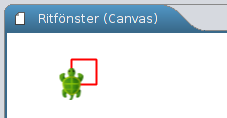
\includegraphics[width=0.45\textwidth]{../img/kojo/kvadrat}
%
%\Subtask Prova olika sätt att skriva din kod \emph{utan} att resultatet ändras: skriv satser i sekvens på flera rader eller satser i sekvens på samma rad med semikolon emellan; använd blanktecken och blanka rader i koden. Hur vill du gruppera dina satser så att de är lätta för en människa att läsa?
%
%\Subtask Prova att ändra på \emph{ordningen} mellan satserna och studera hur resultatet påverkas. Använd den \emph{gula} play-knappen  (programspårning) för att studera exekveringen i detalj. Klicka på satser i ditt program och på rutor i programspårningen och se vad som händer.
%
%
%\Subtask Rita en trappa enligt bilden nedan.
%
%
\includegraphics[width=0.2\textwidth]{../img/kojo/stairs}
%
%\Subtask Rita valfri bild på valfri bakgrund med hjälp av några av procedurerna i tabellen nedan. Du kan till exempel rita en rosa triangel med lila konturer mot svart bakgrund. % \ref{lab:kojo:kojo-procedures}.
%Försök att underlätta läsbarheten av din kod med hjälp av lämpliga radbrytningar och gruppering av satser. Undersök hur ordningen av satserna i din kod påverkar resultatet.
%
%
%
%\begin{table}[H]
%\begin{tabular}{l l}\small
%\code|fram(100)| & Paddan går framåt 100 steg (25 om argument saknas).\\
%\code|färg(rosa)| & Sätter pennans färg till rosa. \\
%\code|fyll(lila)| & Sätter ifyllnadsfärgen till lila. \\
%\code|fyll(genomskinlig)| & Gör så att paddan \emph{inte} fyller i något när den ritar. \\
%\code|bredd(20)| & Gör så att pennan får bredden 20. \\
%\code|bakgrund(svart)| & Bakgrundsfärgen blir svart. \\
%\code|bakgrund2(grön,gul)| & Bakgrund med övergång från grönt till gult. \\
%\code|pennaNer|  & Sätter ner paddans penna så att den ritar när den går. \\
%\code|pennaUpp|  & Sänker paddans penna så att den \emph{inte} ritar när den går. \\
%\code|höger(45)|   & Paddan vrider sig 45 grader åt höger. \\
%\code|vänster(45)| & Paddan vrider sig 45 grader åt vänster. \\
%\code|hoppa|       & Paddan hoppar 25 steg utan att rita. \\
%\code|hoppa(100)|  & Paddan hoppar 100 steg utan att rita. \\
%\code|hoppaTill(100, 200)| & Paddan hoppar till läget (100, 200) utan att rita. \\
%\code|gåTill(100, 200)|    & Paddan vrider sig och går till läget (100, 200). \\
%\code|öster|   & Paddan vrider sig så att nosen pekar åt höger. \\
%\code|väster|  & Paddan vrider sig så att nosen pekar åt vänster. \\
%\code|norr|    & Paddan vrider sig så att nosen pekar uppåt. \\
%\code|söder|   & Paddan vrider sig så att nosen pekar neråt. \\
%\code|mot(100,200)|   & Paddan vrider sig så att nosen pekar mot läget (100, 200) \\
%\code|sättVinkel(90)| & Paddan vrider nosen till vinkeln 90 grader. \\
%\end{tabular}
%%\label{lab:kojo:kojo-procedures}
%%\caption{Några användbara procedurer i Kojo.}
%\end{table}


%%% NEDAN ÄR BORTTAGEN FÖR ATT MINSKA MÄNGDEN ARBETE

%\Subtask \emph{Rita och mät}.
%\begin{itemize}[noitemsep]
%\item Börja ditt program med dessa satser:\\ \code{sudda; axesOn; gridOn; sakta(0); osynlig}
%\item Rita sedan en kvadrat som har 444 längdenheter i omkrets.
%\item Ta fram linjalen med höger-klick i ritfönstret och mät så exakt du kan hur lång diagonalen i kvadraten är. Skriv ner resultatet. \\ \emph{Tips:} Du kan zooma med mushjulet om du håller nere Ctrl-knappen. Du kan flytta linjalen om du klick-drar på linjalens skalstreck. Du kan vrida linjalen om du klickar på skalstrecken och håller nere Shift-tangenten.
%\item Kontrollera med hjälp av \code{math.hypot} och \code{println} vad det exakta svaret är. Skriv ner svaret med 3 decimalers noggrannhet. Du kan t.e.x. använda REPL i ett terminalfönster bredvid, eller öppna ett nytt extra Kojo-fönster i Arkiv-menyn, eller lägga in utskrifterna sist i ditt befintliga program. Utskrifter med \code{println} i Kojo sker i utdatafönstret.
%\end{itemize}
%
%\Subtask Rita en liksidig triangel med sidan 300 längdenheter genom att ge lämpliga argument till \code{fram} och \code{höger}. Vinklar anges i grader.
%
%\Subtask\Checkpoint Visa dina resultat för en handledare och diskutera hur uppgifterna ovan illustrerar principen om sekvens.

\vspace{1em}

% \Task Läs om hur du gör grafikprogram med Kojo i Appendix \ref{appendix:kojo} och övning {\tt \ExeWeekONE} i kapitel \ref{exe:W01}.


\Task \textit{Sekvens och repetition}. Rita en kvadrat med hjälp av \code+upprepa(n){ ??? }+ där du ersätter \code{n} med antalet repetitioner och \code{???} med de satser som ska repeteras.

%\Subtask Om du kör Kojo Desktop: Prova att köra ditt program med den \emph{gula} play-knappen för programspårning. Studera exekveringssekvensen. Klicka på anropen i programspårningsfönstret och studera markeringarna i ritfönstret.





\Task \textit{Variabel och repetition}.

\Subtask Funktionen \code{System.currentTimeMillis} ingår i Javas standardbibliotek och ger ett heltal av typen \code{Long} med det nuvarande antalet millisekunder sedan midnatt den första januari 1970.  Med Kojo-proceduren \code{sakta(0)} blir det ingen fördröjning när paddan ritar och utritningen sker så snabbt som möjligt. Prova nedan program och förklara vad som händer.
\begin{Code}
sakta(0)
val n = 800 * 4
val t1 = System.currentTimeMillis
upprepa(n){ upprepa(4){ fram; höger } }
val t2 = System.currentTimeMillis
println(s"$n kvadratvarv tog ${t2 - t1} millisekunder")
\end{Code}
\noindent Om du kör Kojo Desktop är det bra att börjar programmet med \code{sudda}. (Varför?)

\Subtask\Pen Anteckna ungefär hur många kvadratvarv per sekund som paddan kan rita när den är som snabbast. Kör flera gånger eftersom den virtuella maskinen behöver ''värmas upp'' för att maskinkoden ska optimeras. Vissa körningar kan gå långsammare om skräpsamlaren behöver lägga tid på att frigöra minne.

\Subtask\Pen Vad har variablerna i koden ovan för namn? Vad har variablerna för värden?

\Subtask Rita en kvadrat igen, men nu med hjälp av en \code{while}-sats och en loopvariabel. %Studera exekveringen med programspårning (den gula play-knappen).

\begin{Code}
sakta(100)
var i = 0
while (???) { fram; höger; i = ??? }
\end{Code}

\Subtask\Pen Vad är det för skillnad på variabler som deklareras med \code{val} respektive \code{var}?

\Subtask Rita en kvadrat igen, men nu med hjälp av en \code{for}-sats. Skriv ut värdet på den lokala variabeln \code{i} i varje loop-runda.

\begin{Code}
for (i <- 1 to ???) { ??? }
\end{Code}

\Subtask\Pen Går det att tilldela variabeln \code{i} ett nytt värde i loopen?

\Subtask\Pen Går det att referera till namnet \code{i} utanför loopen?


\Subtask Rita en kvadrat igen, men nu med hjälp av \code{foreach}. Skriv ut loopvariabelns värde i varje runda.

\begin{Code}
(1 to ???).foreach{ i => ??? }
\end{Code}

%\Subtask\Pen För var och en av de fyra repetitionskonstruktionerna du sett ovan, \code{upprepa}, \code{while}, \code{for} och \code{foreach}: skriv kod med penna på papper som skriver ut de första 100 jämna heltalen med blanktecken emellan: \code{2 4 6 8 10 12 ...} etc.\\ Vilken typ av loop tycker du är enklast att använda i detta fall?


\Task \textit{Abstraktion}.

\Subtask Använd en repetition för att abstrahera nedan sekvens, så att programmet blir kortare:
\begin{Code}
fram; höger; hoppa; fram; vänster; hoppa; fram; höger;
hoppa; fram; vänster; hoppa; fram; höger; hoppa; fram;
vänster; hoppa; fram; höger; hoppa; fram; vänster; hoppa;
fram; höger; hoppa; fram; vänster; hoppa
\end{Code}

%\Subtask\Pen Sök på nätet efter ''DRY principle programming'' och beskriv med egna ord vad DRY betyder och varför det är en viktig princip.

\Subtask Definiera en egen procedur som heter \code{kvadrat} med hjälp av nyckelordet \code{def} som vid anrop ritar en kvadrat med hjälp av en \code{for}-loop.

\begin{Code}
def kvadrat = for (???) {???}
\end{Code}


\Subtask Anropa din abstraktion efter att den deklarerats och efter att du exekverat:\\\code{sakta(100)}


\Subtask Anropa din abstraktion inuti en \code{for}-loop så att paddan ritar en stapel som är 10 kvadrater hög enligt bilden nedan.

\begin{figure}
  \begin{multicols}{2}

  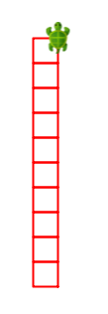
\includegraphics[scale=0.6]{../img/kojo/square-column}

  \columnbreak

  \begin{Code}
  def kvadrat = for (???) {???}
  for (???) {???}
  \end{Code}

  \end{multicols}
  \caption{En kvadratstapel.\label{fig:kojo-lab:column}}
\end{figure}

\Subtask %Kör ditt program med den \emph{gula} play-knappen. 
Studera hur anrop av proceduren \code{kvadrat} påverkar exekveringssekvensen av dina satser genom att göra lämpliga utskrifter så att du kan se när olika delar av koden exekveras. Vid vilka punkter i programmet sker ett ''hopp'' i sekvensen i stället för att efterföljande sats exekveras?  Använd lämpligt argument till \code{sakta} för att du ska hinna studera exekveringen.


\Subtask Rita samma bild med 10 staplade kvadrater (se bild \ref{fig:kojo-lab:column} på sidan \pageref{fig:kojo-lab:column}), men nu \emph{utan} att använda abstraktionen \code{kvadrat} -- använd i stället en nästlad repetition (alltså en upprepning inuti en upprepning). Vilket av de två sätten (med och utan abstraktionen \code{kvadrat}) är lättast att läsa? %\emph{Tips:} Varje gång du trycker på någon av play-knapparna, sparas ditt program. Du kan se dina sparade program om du klickar på \emph{Historik}-fliken. Du kan också stega bakåt och framåt i historiken med de blå pilarna bredvid play-knapparna.

\Subtask Generalisera din abstraktion \code{kvadrat} genom att ge den en parameter \code{sida: Double} som anger hur stor kvadraten blir. Rita flera kvadrater i likhet med bild \ref{fig:kojo-lab:resize} på sidan \pageref{fig:kojo-lab:resize}).

\begin{figure}[H]

\includegraphics{../img/kojo/square-param}
  \caption{Olika stora kvadrater.\label{fig:kojo-lab:resize}}

\end{figure}



%\Subtask\Pen%\Checkpoint
%Se över ditt program i föregående uppgift och säkerställ att det är lättläst och följer en struktur som börjar med alla definitioner i logisk ordning och därefter fortsätter med huvudprogrammet.
%%Diskutera ditt program med en handledare.



%\Subtask\Pen Spara ditt program i en fil men lämpligt namn och ha programmet redo när det är din tur att redovisa vad du gjort under laborationen.
%Anteckna några åtgärder du vidtagit för att göra programmet mer lättläst.







\Task \emph{Alternativ.} \label{kojo:alt}

\Subtask Kör programmet nedan. Förklara vad som händer. %Använd den gula play-knappen för att studera exekveringen.

\begin{Code}
sakta(5000)

def move(key: Int): Unit = {
  println("key: " + key)
  if (key == 87) fram(10)
  else if (key == 83) fram(-10)
}

move(87); move('W'); move('W')
move(83); move('S'); move('S'); move('S')
\end{Code}

\Subtask \label{subtask:keypress}  Kör programmet nedan. Notera \code{activateCanvas} för att du ska slippa klicka i ritfönstret innan du kan styra paddan. Anropet \code{onKeyPress(move)} gör så att \code{move} kommer att anropas då en tangent trycks ned. Lägg till kod i \code{move} som gör att tangenten A ger en vridning moturs med 5 grader medan tangenten D ger en vridning medurs 5 grader. Med \code{onKeyPress} bestämmer man vilken procedur som ska köras vid tangenttryck.

\begin{Code}
sakta(0); activateCanvas

def move(key: Int): Unit = {
  println("key: " + key)
  if (key == 'W') fram(10)
  else if (key == 'S') fram(-10)
}

onKeyPress(move)
\end{Code}



%\Subtask Spara ditt program i en fil men lämpligt namn och ha programmet redo när det är din tur att redovisa vad du gjort under laborationen.


\subsection{Kontrollfrågor}\Checkpoint

\noindent Repetera teorin för denna vecka och var beredd på att kunna svara på dessa frågor när det blir din tur att redovisa vad du gjort under laborationen:

\begin{enumerate}
\item Vad innebär sekventiell exekvering av satser?
\item Vad är skillnaden mellan en sats och ett uttryck?
\item Vad är skillnaden mellan en procedur och en funktion?
\item Spelar ordningen mellan argument någon roll vid anrop av en funktion med flera parametrar?
\item Vad är en variabel? Ge exempel på deklaration, initialisering och tilldelning av variabler, samt användning av variabler i uttryck.
\item Vad är ett logiskt uttryck? Ge exempel på användning av logiska uttryck.
\item Vad är abstraktion? Ge exempel på användning av abstraktion.
\item Vad är nyttan med abstraktion?
\item Vad innebär sidoeffekt? Förklara och ge exempel.
\item Hur deklareras och initialiseras en variabel vars värde är förändringsbart?
\item Hur deklareras och initialiseras en variabel vars värde är oföränderligt?
\item Är det ett körtidsfel eller kompileringsfel att tilldela en oföränderlig variabel ett nytt värde?
\item Ange vilken av \code{for} och \code{while} som är lämpligast i dessa fall:
\begin{itemize}[noitemsep, nolistsep]
\item[A.] Summera de hundra första heltalen.
\item[B.] Räkna antal tecken i en sträng innan första blanktecken.
\item[C.] Dra 100 slumptal mellan 1 och 6 och summera de tal som är mindre än 3.
\item[D.] Summera de första heltalen från 1 och uppåt tills summan är minst 100.
\end{itemize}
\end{enumerate}


\subsection{Frivilliga extrauppgifter}

\noindent Gör i mån intresse och träningsbehov nedan uppgifter i valfri ordning.

\Task \emph{Abstraktion och generalisering}.

\Subtask Skapa en abstraktion \code{def stapel = ???} som använder din abstraktion \code{kvadrat}.

\Subtask Du ska nu \emph{generalisera} din procedur så att den inte bara kan rita exakt 10 kvadrater i en stapel. Ge proceduren \code{stapel} en parameter \code{n} som styr hur många kvadrater som ritas.
\begin{Code}
def kvadrat = ???
def stapel(n: Int) = ???

sakta(100)
stapel(42)
\end{Code}



\Subtask Rita nedan bild med hjälp av abstraktionen \code{stapel}. Det är totalt 100 kvadrater och varje kvadrat har sidan 25. \emph{Tips:} Med ett negativt argument till procedur \code{hoppa} kan du få sköldpaddan att hoppa baklänges utan att rita, t.ex. \code{hoppa(-10*25)}

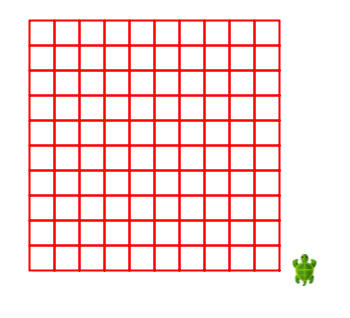
\includegraphics[width=0.3\textwidth]{../img/kojo/square-grid}

\Subtask Generalisera dina abstraktioner \code{kvadrat} och \code{stapel} så att man kan påverka storleken på kvadraterna som ritas ut.

\Subtask Skapa en abstraktion \code{rutnät} med lämpliga parametrar som gör att man kan rita rutnät med olika stora kvadrater och olika många kvadrater i både x- och y-led.

\Subtask Generalisera dina abstraktioner \code{kvadrat} och \code{stapel} så att man kan påverka fyllfärgen och pennfärgen för kvadraterna som ritas ut.

\Task \emph{Växling med booleska värden.}

\Subtask Bygg vidare på programmet i uppgift \ref{kojo:alt} och lägg till nedan kod i början av programmet. Lägg även till kod som gör så att om man trycker på tangenten G så sätts rutnätet omväxlande på och av. Observera att det är exakt \emph{en} procedur som anropas vid \code{onKeyPress}.

\begin{Code}
var isGridOn = false

def toggleGrid =
  if (isGridOn) {
    gridOff
    isGridOn = false
  } else {
    gridOn
    isGridOn = true
  }
\end{Code}

\Subtask Gör så att när man trycker på tangenten X så sätter man omväxlande på och av koordinataxlarna. Använd en variabel \code{isAxesOn} och definiera en abstraktion \code{toggleAxes} som anropar \code{axesOn} och \code{axesOff} på liknande sätt som i föregående uppgift.


\Task \emph{Repetition.}~Skriv en procedur \code{randomWalk} med detta huvud: \\
\code{def randomWalk(n: Int, maxStep: Int, maxAngle: Int): Unit}\\ som gör så att paddan tar \code{n} steg av slumpmässig längd mellan \code{0} och \code{maxStep}, samt efter varje steg vrider sig åt vänster en slumpmässig vinkel mellan \code{0} och \code{maxAngle}. Anropa din procedur med olika argument och undersök hur dess värden påverkar bildens utseende. \emph{Tips:} Uttrycket \code{math.random() * 100} ger ett tal från 0 till (nästan) 100. Du kan styra hur långsamt paddan ritar genom anrop av \code{sakta(???)} (prova dig fram till något  lämpligt heltalsargument i stället för \code{???}).
\vspace{2em}\\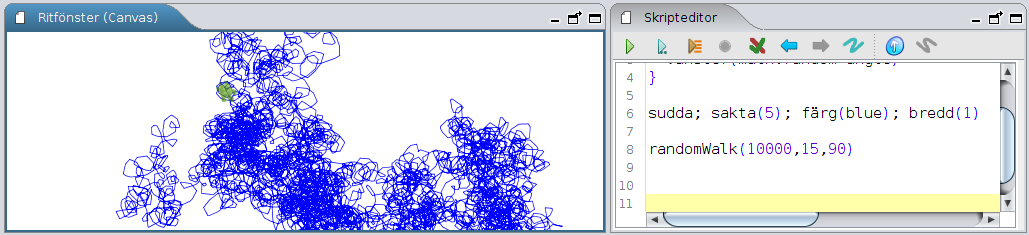
\includegraphics[width=\textwidth]{../img/kojo/random-walk.png}


\Task \emph{Variabler, namngivning och formatering.}

\Subtask Klistra in nedan konstigt formatterade program \emph{exakt} som det står med blanktecken, indragningar och radbrytningar. Kör programmet och förklara vad som händer.

\begin{figure}[H]
\begin{Code}
// Ett konstigt formaterat program med en del konstiga namn.

def gurka(x: Double,
y: Double, namn: String,
typ: String,
värde:String) = {
val tomat = 15
val h = 30
hoppaTill(x,y)
norr
skriv(namn+": "+typ)
hoppaTill(x+tomat*(namn.size+typ.size),y)
skriv(värde); söder; fram(h); vänster
fram(tomat * värde.size); vänster
fram(h); vänster
fram(tomat * värde.size); vänster }
sudda; färg(svart); val s = 130
val h = 40
var x = 42; gurka(10, s-h*0, "x","Int", x.toString)
var y = x; gurka(10, s-h*1, "y","Int", y.toString)
x = x + 1; gurka(10, s-h*2, "x","Int", x.toString)
gurka(10, s-h*3, "y","Int", y.toString); osynlig
\end{Code}
\end{figure}

\Subtask\Pen Skriv ner namnet på alla variabler som förekommer i programmet.

\Subtask\Pen Vilka av dessa variabler är lokala?

\Subtask\Pen Vilka av dessa variabler kan förändras efter initialisering?

\Subtask\Pen Föreslå tre förändringar av programmet ovan (till exempel namnbyten) som gör att det blir lättare att läsa och förstå.

\Subtask Gör sök-ersätt av \code{gurka} till ett bättre namn. \emph{Tips:} undersök kontextmenyn i editorn i Kojo genom att högerklicka. Använd kortkommandot för Sök/Ersätt.

\Subtask Gör automatisk formatering av koden med hjälp av lämpligt kortkommando. Notera skillnaderna. Vilka autoformateringar gör programmet lättare att läsa? Vilka manuella formateringar tycker du bör göras för att öka läsbarheten? Ge funktionen \code{gurka} ett bättre namn.  Diskutera läsbarheten med en handledare.



\Task \label{task:measuretime} \emph{Tidmätning.} Hur snabb är din dator?

\Subtask \label{task:timer} Skriv in koden nedan i Kojos editor och kör upprepade gånger med den gröna play-knappen. Tar det lika lång tid varje gång? Varför?

\begin{Code}
object timer {
  def now: Long = System.currentTimeMillis
  var saved: Long = now
  def elapsedMillis: Long = now - saved
  def elapsedSeconds: Double = elapsedMillis / 1000.0
  def reset: Unit = { saved = now }
}

// HUVUDPROGRAM:
timer.reset
var i = 0L
while (i < 1e8.toLong) { i += 1 }
val t = timer.elapsedSeconds
println("Räknade till " + i + " på " + t + " sekunder.")
\end{Code}


\Subtask Ändra i loopen i uppgift \ref{task:timer}) så att den räknar till 4.4 miljarder. Hur lång tid tar det för din dator att räkna så långt?\footnote{Det går att göra ungefär en heltalsaddition per klockcykel per kärna. Den första elektroniska datorn \href{https://sv.wikipedia.org/wiki/ENIAC}{Eniac} hade en klockfrekvens motsvarande 5 kHz. Den dator på vilken denna övningsuppgift skapades hade en i7-4790K turboklockad upp till 4.4 GHz.
%\href{http://www.extremetech.com/computing/185512-overclocking-intels-core-i7-4790k-can-devils-canyon-fix-haswells-low-clock-speeds/2}{www.extremetech.com/computing/185512-overclocking-intels-core-i7-4790k-can-devils-canyon-fix-haswells-low-clock-speeds/2}
}

\Subtask  Om du kör på en Linux-maskin: Kör nedan Linux-kommando upprepade gånger i ett terminalfönster. Med hur många MHz kör din dators klocka för tillfället? Hur förhåller sig klockfrekvensen till antalet rundor i while-loopen i föregående uppgift? (Det kan hända att din dator kan variera centralprocessorns klockfrekvens. Prova både medan du kör tidmätningen i Kojo och då din dator ''vilar''. Vad är det för poäng med att en processor kan variera sin klockfrekvens?)
\begin{REPLnonum}
> lscpu | grep MHz
\end{REPLnonum}


\Subtask Ändra i koden i uppgift \ref{task:timer}) så att \code{while}-loopen bara kör 5 gånger. %Kör programmet med den \emph{gula} play-knappen. Scrolla i programspårningen och förklara vad som händer. Klicka på \code{CALL}-rutorna och se vilken rad som markeras i ditt program.

\Subtask Lägg till koden nedan i ditt program och försök ta reda på ungefär hur långt din dator hinner räkna till på en sekund för \code{Long}- respektive \code{Int}-variabler. Använd den gröna play-knappen.
\begin{CodeSmall}
def timeLong(n: Long): Double = {
  timer.reset
  var i = 0L
  while (i < n) { i += 1 }
  timer.elapsedSeconds
}

def timeInt(n: Int): Double = {
  timer.reset
  var i = 0
  while (i < n) { i += 1 }
  timer.elapsedSeconds
}

def show(msg: String, sec: Double): Unit = {
  print(msg + ": ")
  println(sec + " seconds")
}

def report(n: Long): Unit = {
  show("Long " + n, timeLong(n))
  if (n <= Int.MaxValue) show("Int  " + n, timeInt(n.toInt))
}

// HUVUDPROGRAM, mätningar:

report(Int.MaxValue)
for (i <- 1 to 10) report(4.26e9.toLong)
\end{CodeSmall}

\Subtask Hur mycket snabbare går det att räkna med \code{Int}-variabler jämfört med \code{Long}-variabler? Diskutera gärna svaret med en handledare.

\Task Lek med färg i Kojo. Sök på internet efter dokumentationen för klassen \code{java.awt.Color} och studera vilka heltalsparametrar den sista konstruktorn i listan med konstruktorer tar för att skapa sRGB-färger. Om du högerklickar i editorn i Kojo och väljer ''Välj färg...'' får du fram färgväljaren och med den kan du välja fördefinierade färger eller blanda egna färger. När du har valt färg får du se vilka parametrar till \code{java.awt.Color} som skapar färgen. Testa detta i REPL:

\begin{REPL}
scala> val c = new java.awt.Color(124,10,78,100)
c: java.awt.Color = java.awt.Color[r=124,g=10,b=78]

scala> c.  // tryck på TAB
asInstanceOf    getColorComponents      getRGBComponents
brighter        getColorSpace           getRed
createContext   getComponents           getTransparency
darker          getGreen                isInstanceOf
getAlpha        getRGB                  toString
getBlue         getRGBColorComponents

scala> c.getAlpha
res3: Int = 100
\end{REPL}
Skriv ett program som ritar många figurer med olika färger, till exempel cirklar som nedan. Om du använder alfakanalen blir färgerna genomskinliga.

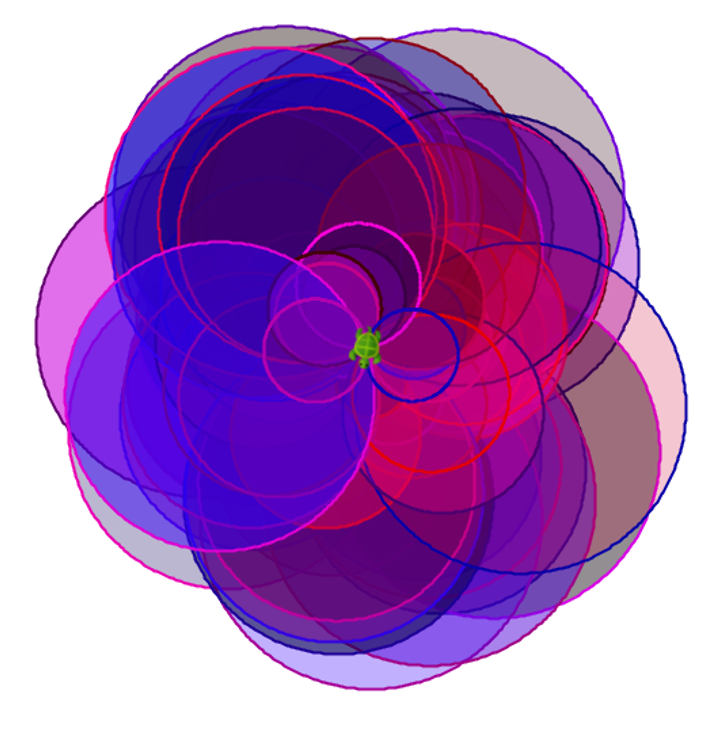
\includegraphics[width=0.82\textwidth]{../img/kojo/random-color-circles.png}


\Task Ladda ner ''Uppdrag med Kojo'' från \href{http://lth.se/programmera/uppdrag}{lth.se/programmera/uppdrag}  och gör några uppgifter som du tycker verkar intressanta.

%\Subtask ''Programming Fundamentals with Kojo'' som kan laddas ner här:\\
%\href{http://wiki.kogics.net/kojo-codeactive-books}{wiki.kogics.net/kojo-codeactive-books}

\Task Om du vill jobba med att hjälpa skolbarn att lära sig programmera med Kojo, kontakta \url{http://www.vattenhallen.lth.se} och anmäl ditt intresse att vara handledare.


%!TEX encoding = UTF-8 Unicode
%!TEX root = ../compendium1.tex

\renewcommand{\vecka}{2}

\chapter{Kodstrukturer}\label{chapter:W02}
\begin{itemize}[nosep]
\item samling: Range
\item for-uttryck
\item map
\item foreach
\item flatMap
\item algoritm vs implementation
\item pseudokod
\item algoritm: swap
\item algoritm: summering
\item algoritm: min/max
\item paket
\item import
\item filstruktur
\item jar
\item dokumentation
\item programlayout
\item JDK
\item konstanter vs föränderlighet
\item objektorientering
\item klasser
\item objekt
\item punktnotation
\item referensvariabler
\item referenstilldelning
\item anropa metoder
\item block
\item namnsynlighet
\item namnöverskuggning
\item SimpleWindow
\end{itemize}

%!TEX encoding = UTF-8 Unicode
%!TEX root = ../lect-week02.tex

%\Subsection{Samlingar och loopar}
\Subsection{Datastrukturer och kontrollstrukturer}


\begin{Slide}{Vad är en datastruktur?}\SlideFontSmall
\begin{itemize}
\item En \href{https://sv.wikipedia.org/wiki/Datastruktur}{datastruktur} är en struktur för organisering av data som...
\begin{itemize}\SlideFontTiny
\item kan innehålla \Alert{många} element,
\item kan refereras till med \Alert{ett} enda namn, och
\item ger möjlighet att komma åt de enskilda elementen.
\end{itemize}

\item En \Emph{samling} \Eng{collection} är en datastruktur som kan innehålla många element av \Alert{samma typ}.

\item Exempel på olika samlingar där elementen är organiserade på olika vis: \\ 
\vspace{0.5em}
\begin{tabular}{l c}
\Emph{Lista} & 
\includegraphics[width=5cm]{../img/list.pdf} \\
\Emph{Träd}  & 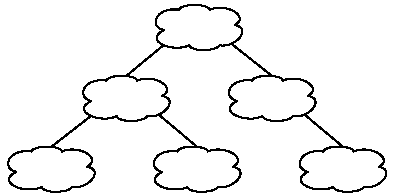
\includegraphics[width=2.2cm]{../img/tree.pdf} \\
\Emph{Graf}  & 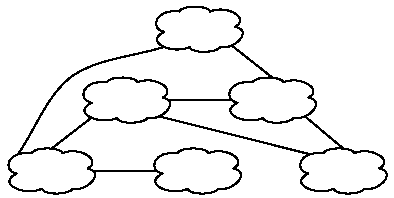
\includegraphics[width=2.2cm]{../img/graph.pdf} \\
\end{tabular}
\end{itemize}
{
\SlideFontTiny \vspace{1em }\hskip2em
Mer om listor \& träd \href{http://cs.lth.se/edaa01vt}{fördjupningskursen}. 
Mer om träd, grafer i \href{http://cs.lth.se/edaa40}{Diskreta strukturer.}
}

\end{Slide} 


\begin{Slide}{Vad är en vektor?}\SlideFontSmall
En \Emph{vektor}\footnote{Vektor kallas ibland på svenska även \href{https://sv.wikipedia.org/wiki/F\%C3\%A4lt_\%28datastruktur\%29}{fält}, men det skapar stor förvirring eftersom det engelska ordet \emph{field} ofta används för \emph{attribut} (förklaras senare).} 
\Eng{vector, \href{https://en.wikipedia.org/wiki/Array_data_structure}{array}} är en \Emph{samling} som är \Alert{snabb} att \Emph{indexera} i. 
Åtkomst av element sker med \code{apply(platsnummer)}: 

\begin{REPL}
scala> val heltal = Vector(42, 13, -1, 0 , 1)
heltal: scala.collection.immutable.Vector[Int] = Vector(42, 13, -1, 0, 1)

scala> heltal.apply(0)
res0: Int = 42

scala> heltal(1)    // man kan skippa .apply
res1: Int = 13

scala> heltal(5)
java.lang.IndexOutOfBoundsException: 5
  at scala.collection.immutable.Vector.checkRangeConvert(Vector.scala:132)
\end{REPL}
Utelämnar du \code{.apply} så gör kompilatorn anrop av \code{apply} ändå om det går.
\end{Slide}

\begin{Slide}{En konceptuell bild av en vektor}

\begin{REPLnonum}
scala> val heltal = Vector(42, 13, -1, 0 , 1)

scala> heltal(0)
res0: Int = 42
\end{REPLnonum}

\begin{tikzpicture}[font=\ttfamily]
\matrix [matrix of nodes, row sep=0, column 2/.style={nodes={rectangle,draw,minimum width=3em}}] (var) at (0cm, 2.8cm)
{
heltal   &  \makebox(16,12){ }\\
};
\matrix [matrix of nodes, draw=black,row sep=0, column 2/.style={nodes={rectangle,draw,minimum width=4em}}] (vec) at (4cm, 1cm)
{
\textit{plats} &  \\
0   &  \makebox(16,12){42}\\
1   &  \makebox(16,12){13}\\
2   &  \makebox(16,12){-1}\\
3   &  \makebox(16,12){0}\\
4   &  \makebox(16,12){1}\\
};
\filldraw[black] (0.7cm,2.8cm) circle (3pt) node[] (ref) {};
 \draw [arrow] (ref) -- (vec);
\end{tikzpicture}

%\vspace{1em} Elementen ligger på rad någonstans i minnet.
\end{Slide}



\begin{Slide}{En samling strängar}

\begin{itemize}
\item En vektor kan lagra många värden av samma typ. 
\item Elementen kan vara till exempel heltal eller strängar. 
\item Eller faktiskt vad som helst. 
\end{itemize}

\begin{REPL}
scala> val grönsaker = Vector("gurka","tomat","paprika","selleri")
grönsaker: scala.collection.immutable.Vector[String] = Vector(gurka, tomat, paprika, selleri)

scala> val g = grönsaker(1)
g: String = tomat

scala> val xs = Vector(42, "gurka", true, 42.0)
xs: scala.collection.immutable.Vector[Any] = Vector(42, gurka, true, 42.0)


\end{REPL}

\end{Slide}

\begin{Slide}{Vad är en kontrollstruktur?}
\begin{itemize}
\item En \Emph{kontrollstruktur} påverkar \Alert{sekvensen}.
\begin{itemize}
\item[] Exempel på inbyggda kontrollstrukturer: 
\\\vspace{0.5em}\code{for}-sats, \code{while}-sats
\end{itemize}

\item[]

\item I Scala kan man definiera \Emph{egna} kontrollstrukturer.
\begin{itemize}
\item[] Exempel: \code{upprepa} som du använt i Kojo
\\\vspace{0.5em}\code|upprepa(4){fram; höger}|
\end{itemize}
\end{itemize}
\end{Slide}


\begin{Slide}{Mitt första program: en oändlig loop på ABC80}
\begin{columns}
\begin{column}{0.8\textwidth}
\begin{verbatim}
10 print "hej"
20 goto 10
\end{verbatim}
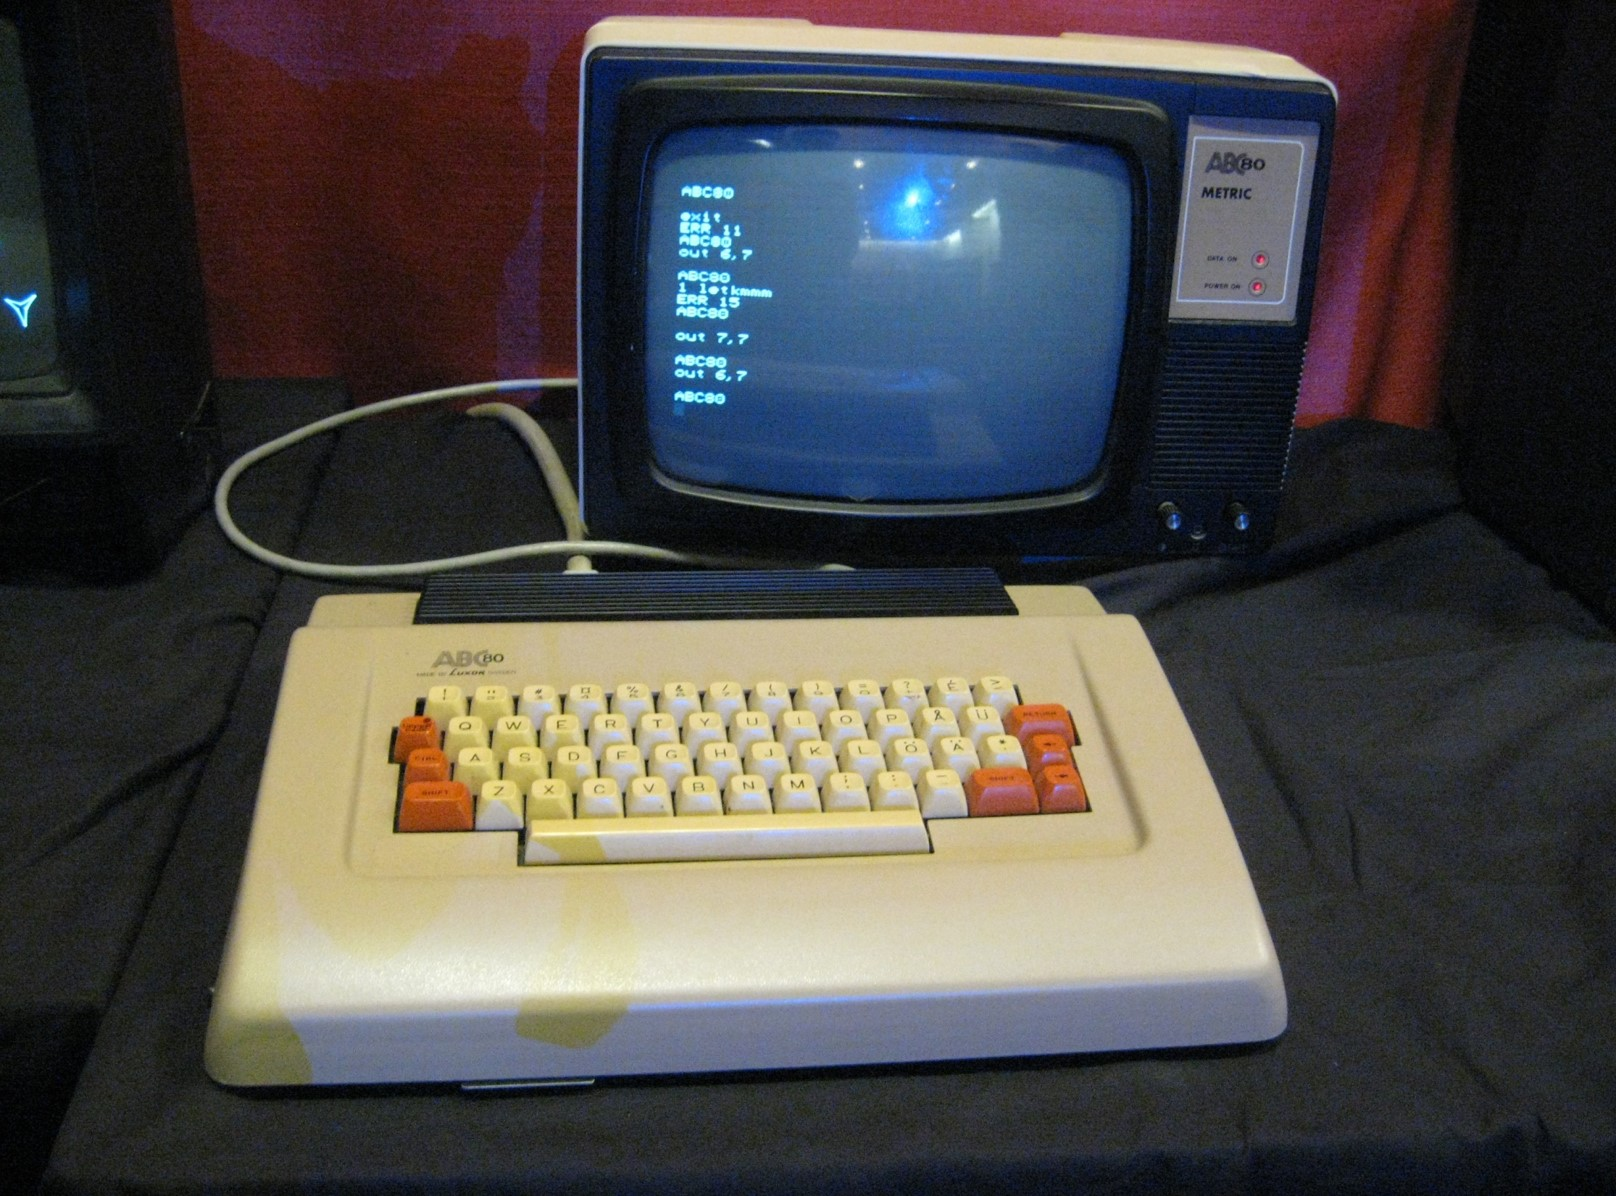
\includegraphics[width=0.8\textwidth]{../img/abc80.jpg}
\end{column}
\begin{column}{0.3\textwidth}
\pause
\begin{verbatim}
hej
hej
hej
hej
hej
hej
hej
hej
hej
hej
hej
hej
<Ctrl+C>
\end{verbatim}

\end{column}
\end{columns}
\end{Slide}


\begin{Slide}{Loopa genom elementen i en vektor}
En \code{for}-\Emph{sats} som skriver ut alla element i en vektor:
\begin{REPL}
scala> val grönsaker = Vector("gurka","tomat","paprika","selleri")

scala> for (g <- grönsaker) println(g)
gurka
tomat
paprika
selleri

\end{REPL}

\end{Slide}


\begin{Slide}{Bygga en ny samling från en befintlig med for-uttryck}
Ett \code{for}-\code{yield}-\Emph{uttryck} som \Emph{skapar en \Alert{ny} samling}.

\begin{Code}[basicstyle=\ttfamily\fontsize{12}{14}\selectfont]
for (g <- grönsaker) yield "god " + g
\end{Code}

\begin{REPL}
scala> val grönsaker = Vector("gurka","tomat","paprika","selleri")

scala> for (g <- grönsaker) yield "god " + g
res0: scala.collection.immutable.Vector[String] = 
  Vector(god gurka, god tomat, god paprika, god selleri)

scala> val åsikter = for (g <- grönsaker) yield s"god $g"
åsikter: scala.collection.immutable.Vector[String] = 
  Vector(god gurka, god tomat, god paprika, god selleri)
\end{REPL}

\end{Slide}


\begin{Slide}{Samlingen \code{Range} håller reda på intervall}
\begin{itemize}
\item Med en \code{Range(start, slut)} kan du skapa ett intervall: \\ från och med \code{start} till (men inte med) \code{slut}
\end{itemize}

\begin{REPLnonum}
scala> Range(0, 42)
res0: scala.collection.immutable.Range = 
  Range(0, 1, 2, 3, 4, 5, 6, 7, 8, 9, 10, 11, 12, 13, 14, 
    15, 16, 17, 18, 19, 20, 21, 22, 23, 24, 25, 26, 27, 28, 
    29, 30, 31, 32, 33, 34, 35, 36, 37, 38, 39, 40, 41)
\end{REPLnonum}

\begin{itemize}
\item Men alla värden däremellan skapas inte förrän de behövs:
\end{itemize}

\begin{REPL}
scala> val jättestortIntervall = Range(0, Int.MaxValue)
jättestortIntervall: scala.collection.immutable.Range = Range(0, 1, 2, 3, 4, 5, ...

scala> jättestortIntervall.end
res1: Int = 2147483647

scala> jättestortIntervall.toVector
java.lang.OutOfMemoryError: GC overhead limit exceeded
\end{REPL}

\end{Slide}

\begin{Slide}{Loopa med Range}
\code{Range} används i for-lopar för att hålla reda på antalet rundor.
\begin{REPLnonum}
scala> for (i <- Range(0, 6)) print(" gurka " + i)
 gurka 0 gurka 1 gurka 2 gurka 3 gurka 4 gurka 5 
\end{REPLnonum}
Du kan skapa en \code{Range} med \code{until} efter ett heltal:
\begin{REPLnonum}
scala> 1 until 7
res1: scala.collection.immutable.Range = 
  Range(1, 2, 3, 4, 5, 6)

scala> for (i <- 1 until 7) print(" tomat " + i) 
 tomat 1 tomat 2 tomat 3 tomat 4 tomat 5 tomat 6

\end{REPLnonum}
\end{Slide}

\begin{Slide}{Loopa med Range skapad med \texttt{to}}

Med \code{to} efter ett heltal får du en \code{Range} till och \Emph{med} sista:
\begin{REPLnonum}
scala> 1 to 6
res2: scala.collection.immutable.Range.Inclusive = 
  Range(1, 2, 3, 4, 5, 6)

scala> for (i <- 1 to 6) print(" gurka " + i) 
 gurka 1 gurka 2 gurka 3 gurka 4 gurka 5 gurka 6
 
\end{REPLnonum}


\end{Slide}



\begin{Slide}{Vad är en \code{Array} i JVM?}


\begin{itemize}
\item En \code{Array} liknar en \code{Vector} men har en särställning i JVM:
\begin{itemize}
\item Lagras som en sekvens i minnet på efterföljande adresser.
\item \Emph{Fördel}: snabbaste samlingen för element-access i JVM.
\item Men det finns en hel del \Alert{nackdelar} som vi ska se senare.
\end{itemize}

\end{itemize}

\begin{REPLnonum}
scala> val heltal = Array(42, 13, -1, 0 , 1)
\end{REPLnonum}

\begin{tikzpicture}[font=\ttfamily,scale=0.75, every node/.style={scale=0.75}]
\matrix [matrix of nodes, row sep=0, column 2/.style={nodes={rectangle,draw,minimum width=3em}}] (var) at (0cm, 2.8cm)
{
heltal   &  \makebox(16,12){ }\\
};
\matrix [matrix of nodes, draw=black,row sep=0, column 2/.style={nodes={rectangle,draw,minimum width=4em}}] (vec) at (4cm, 1cm)
{
\textit{plats} &  \\
0   &  \makebox(16,12){42}\\
1   &  \makebox(16,12){13}\\
2   &  \makebox(16,12){-1}\\
3   &  \makebox(16,12){0}\\
4   &  \makebox(16,12){1}\\
};
\filldraw[black] (0.7cm,2.8cm) circle (3pt) node[] (ref) {};
 \draw [arrow] (ref) -- (vec);
\end{tikzpicture}
\end{Slide}

\begin{Slide}{Några likheter \& skillnader mellan \texttt{Vector} och \texttt{Array}}\SlideFontSmall
\begin{multicols}{2}
\begin{REPL}[numbers=none]
scala> val xs = Vector(1,2,3)
\end{REPL}

\columnbreak

\begin{REPL}[numbers=none]
scala> val xs = Array(1,2,3)
\end{REPL}
\end{multicols}


Några likheter mellan \texttt{Vector} och \texttt{Array}
\begin{itemize}
\item Båda är samlingar som kan innehålla många element.

\item Med båda kan man snabbt accessa vilket element som helst: \code{xs(2)}

\item Båda har en fix storlek efter allokering.
\end{itemize}

Några viktiga skillnader:
\begin{multicols}{2}
\Emph{Vector}
\begin{itemize}
\item Är \Emph{oföränderlig}: du kan lita på att elementreferenserna aldrig någonsin kommer att ändras.

\item Är \Emph{snabb på att skapa en delvis förändrad kopia}, t.ex. tillägg/borttagning/uppdatering mitt i sekvensen.

\end{itemize}


\columnbreak

\Alert{Array}
\begin{itemize}
\item Är \Alert{föränderlig}: \code{xs(2) = 42}

\item Är \Alert{snabb} om man bara vill läsa eller skriva på befintliga platser.

\item Är \Alert{långsam} om man vill lägga till eller ta bort element mitt i sekvensen.

\end{itemize}
\end{multicols}
\end{Slide}



\Subsection{Huvudprogram med \texttt{main} i Scala och Java}

\begin{Slide}{Ett minimalt fristående program i Scala och Java}
Nedan Scala-kod skrivs i en editor, spara med valfritt filnamn:
\begin{Code}
// this is Scala 

object Hello {
  def main(args: Array[String]): Unit = {
    println("Hejsan scala-appen!")
  }
}
\end{Code}

\pause
\vspace{1em}
Nedan Java-kod skrivs i en editor, filen \Alert{måste} heta \texttt{Hi.java}

\begin{Code}[language=Java]
// this is Java 

public class Hi {
    public static void main(String[] args) {
        System.out.println("Hejsan Java-appen!");
    }
}
\end{Code}

\end{Slide}


\begin{Slide}{Loopa genom en samling med en \texttt{while}-sats}
\begin{REPLnonum}
scala> val xs = Vector("Hej","på","dej","!!!")
xs: scala.collection.immutable.Vector[String] = 
  Vector(Hej, på, dej, !!!)

scala> xs.size
res0: Int = 4

scala> var i = 0
i: Int = 0

scala> while (i < xs.size) { println(xs(i)); i = i + 1 }
Hej
på
dej
!!!
\end{REPLnonum}
\end{Slide}


\begin{Slide}{Loopa genom argumenten i ett Scala-huvudprogram}
Skriv denna kod och spara i filen \texttt{helloargs.scala}
\begin{REPL}[numbers=none]
$ gedit helloargs.scala
\end{REPL}
\begin{Code}
object HelloScalaArgs {
  def main(args: Array[String]): Unit = {
    var i = 0
    while (i < args.size) { 
      println(args(i))
      i = i + 1
    }
  }
}
\end{Code}
Kompilera och kör:
\begin{REPL}
$ scalac helloargs.scala
$ scala HelloScalaArgs hej gurka tomat 
hej
gurka
tomat
\end{REPL}
\end{Slide}


\begin{Slide}{Loopa genom argumenten i ett Java-huvudprogram}
\begin{REPL}[numbers=none]
$ gedit HelloJavaArgs.java
\end{REPL}
\begin{Code}[language=Java]
// this is Java 

public class HelloJavaArgs {
    public static void main(String[] args) {
    int i = 0;
    while (i < args.length) { 
      System.out.println(args[i]);
      i = i + 1;
    }
  }
}
\end{Code}
Kompilera och kör:
\begin{REPL}
$ javac HelloJavaArgs.scala
$ java HelloJavaArgs hej gurka tomat 
hej
gurka
tomat
\end{REPL}

\end{Slide}


\begin{Slide}{Scala-skript}
\begin{itemize}
\item Skala-kod kan köras som ett \Emph{skript}.\footnote{\SlideFontTiny Du får prova detta på övningen. Vi kommer mest att köra kompilerat i kursen, då Scala-skript saknar mekanism för inkludering av andra skript. Men det finns ett öppenkällkodsprojekt som löser det: \url{http://www.lihaoyi.com/Ammonite/}
}
\item Ett skript kompileras varje gång innan det körs och maskinkoden sparas inte som vid vanlig kompilering.
\item Då behövs ingen \code{main} och inget \code{object}
\end{itemize}

\begin{Code}[basicstyle=\ttfamily\fontsize{10}{12}\selectfont]
// spara nedan i filen 'myscript.scala'

println("Hejsan argumnet!")
for (arg <- args) println(arg)
\end{Code}

\begin{REPLnonum}
$ scala myscript.scala
\end{REPLnonum}


\end{Slide}



\Subsection{Algoritmer: stegvisa lösningar}

\begin{Slide}{Vad är en algoritm?}
En \href{https://sv.wikipedia.org/wiki/Algoritm}{algoritm} är en sekvens av instruktioner som beskriver \\hur man löser ett problem.\\
\vspace{1em}
\Emph{Exempel}: 
\begin{itemize}
\item	 baka en kaka 
\pause\item räkna ut din pensionsprognos 
\pause\item köra bil 
\pause\item kolla om highscore i ett spel 
\item ...
\end{itemize}

\begin{tikzpicture}[overlay]
\node[xshift=0.85\textwidth, scale=2.0] at (0,1.3) { 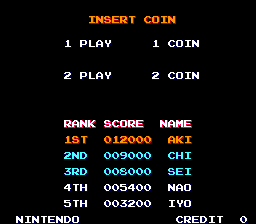
\includegraphics[width=0.25\textwidth]{../img/highscore}};
\end{tikzpicture}
\end{Slide}



\begin{Slide}{Algoritm-exempel: HIGHSCORE}
\Emph{Problem}: Kolla om high-score i ett spel \\ \vspace{1em}

\Emph{Varför?} \pause Så att de som spelar uppmuntras att spela mer :) \\ \vspace{1em}

\Emph{Algoritm:}\pause
\begin{enumerate}
\item $points$ $\leftarrow$ poängen efter senaste spelet
\item $highscore$ $\leftarrow$ bästa resultatet innan senaste spelet
\item \Key{om} $points$ är större än $highscore$ 
\begin{enumerate}[ ~~]
\item  Skriv ''Försök igen!''
\end{enumerate}
\Key{annars}
\begin{enumerate}[ ~~]
\item  Skriv ''Grattis!''
\end{enumerate}
\end{enumerate}
\pause
\scriptsize \Alert{Hittar du buggen?}
\end{Slide}


\begin{Slide}{HIGHSCORE implementerad i Scala}
\begin{Code}
import scala.io.StdIn.readLine

object HighScore {
  def main(args: Array[String]): Unit = {
    val points = readLine("Hur mång poäng fick du?").toInt
    val highscore = readLine("Vad var highscore före senaste spelet?").toInt
    val msg = if (points > highscore) "GRATTIS!" else "Försök igen!"
    println(msg) 
  }
}
\end{Code}
\pause
Är det en bugg eller en feature att det står\\ \texttt{points > highscore} \\ och inte \\ \texttt{points >= highscore} \\ ?
% Buggen är att man inte får GRATTIS om poäng == highscore vilket är tråkigt :)
\end{Slide}


\begin{Slide}{HIGHSCORE implementerad i Java}
\begin{Code}[language=Java]
import java.util.Scanner;

public class HighScore {
    public static void main(String[] args){
        Scanner scan = new Scanner(System.in);
        System.out.println("Hur många poäng fick du?");
        int points =  scan.nextInt();
        System.out.println("Vad var higscore före senaste spelet?");
        int highscore = scan.nextInt();
        if (points > highscore) {
            System.out.println("GRATTIS!");
        } else {
            System.out.println("Försök igen!");
        }
    }
}
\end{Code}
\end{Slide}


\begin{Slide}{Algoritmexempel: N-FAKULTET}
\begin{algorithm}[H]
 \SetKwInOut{Input}{Indata}\SetKwInOut{Output}{Resultat}

 \Input{heltalet $n$}
 \Output{utskrift av produkten av de första $n$ heltalen }
 ~\\
 $prod \leftarrow 1$ \\
 $i \leftarrow 2$  \\
 \While{$i \leq n$}{
  $prod \leftarrow prod * i$\\
  $i \leftarrow i + 1$
 }
 skriv ut $prod$
\end{algorithm}
\pause\vspace{1em}
\begin{itemize}\SlideFontSmall
\item Vad händer om $n$ är noll?
\item Vad händer om $n$ är ett?
\item Vad händer om $n$ är två?
\item Vad händer om $n$ är tre?
\end{itemize}
\end{Slide}

\begin{Slide}{Algoritmexempel: MIN}
\begin{algorithm}[H]
 \SetKwInOut{Input}{Indata}\SetKwInOut{Output}{Resultat}

 \Input{Array $args$ med strängar som alla innehåller heltal}
 \Output{utskrift av minsta heltalet }
 ~\\
 $min \leftarrow$ det största heltalet som kan uppkomma  \\
 $n \leftarrow $ antalet heltal \\
 $i \leftarrow 0$ \\
 \While{$i < n$}{
   $x \leftarrow args(i).toInt$ \\
   \If{( x < $min$)}{$min \leftarrow x$}
   $i \leftarrow i + 1$
 }
 skriv ut $min$
\end{algorithm}
\pause{\hfill \SlideFontTiny \Emph{Test med indata}: \code{args = Array("2", "42", "1", "2")}}
\end{Slide}


\Subsection{Funktioner skapar struktur}

\begin{Slide}{Mall för funktionsdefinitioner}

\code{def} funktionsnamn(parameterdeklarationer): returtyp = block

\pause\vspace{0.5em}\Emph{Exempel}:

\begin{Code}[basicstyle=\ttfamily\fontsize{9}{11}\selectfont]
def öka(i: Int): Int = { i + 1 }
\end{Code}
\pause Om ett enda uttryck: behövs inga \code|{}|. Returtypen kan härledas.
\begin{Code}[basicstyle=\ttfamily\fontsize{9}{11}\selectfont]
def öka(i: Int) = i + 1  
\end{Code}
\pause Om flera parametrar, separera dem med kommatecken: 
\begin{Code}[basicstyle=\ttfamily\fontsize{9}{11}\selectfont]
def isHighscore(points: Int, high: Int): Boolean = {
  val highscore: Boolean = points > high
  if (highscore) println(":)") else print(":(")
  highscore
}
\end{Code}
\pause Ovan funktion har \Alert{sidoeffekten} att skriva ut en smiley.
\end{Slide}

\begin{Slide}{Bättre många små abstraktioner som gör en sak var}

\begin{Code}[basicstyle=\ttfamily\fontsize{8}{11}\selectfont]
def isHighscore(points: Int, high: Int): Boolean = points > high

def printSmiley(isHappy: Boolean): Unit = 
  if (isHappy) println(":)") else print(":(")
\end{Code}

\pause\vspace{2em}
\begin{REPLnonum}
  printSmiley(isHighscore(113,99))
\end{REPLnonum}

\pause\vspace{2em} \code{isHigscore} är en \Emph{äkta funktion} som alltid ger samma svar för samma inparametrar och saknar \Alert{sidoeffekter}.

\end{Slide}



\begin{Slide}{Vad är ett block?}

\begin{itemize}
\item Ett block \Emph{kapslar in} flera satser/uttryck och ser ''utifrån'' ut som en enda sats/uttryck.

\item Ett block skapas med hjälp av klammerparenteser (''krullparenteser'')

\item [] {\fontsize{14}{18}\selectfont \code|{ uttryck1; uttryck2; ... uttryckN }|}\\~

\pause

\item I Scala (till skillnad från många andra språk) har ett block ett \Emph{värde} och är alltså ett \Emph{uttryck}. 

\item Värdet ges av \Emph{sista uttrycket}.

\begin{REPLnonum}
scala> val x = { println(1 + 1); println(2 + 2); 3 + 3 } 
2
4
x: Int = 6
\end{REPLnonum}


\end{itemize}

\end{Slide}

\begin{Slide}{Namn i block blir \textbf{lokala}}
Synlighetsregler: 
\begin{enumerate}
\item Identifierare deklarerade inuti ett block blir \Emph{lokala}.

\item Lokala namn \Alert{överskuggar} namn i yttre block om samma.


\item Namn syns i nästlade underblock.

\end{enumerate}

\begin{REPL}
scala> { val lokaltNamn = 42; println(lokaltNamn) }
42

scala> println(lokaltNamn)
<console>:12: error: not found: value lokaltNamn
       println(lokaltNamn)

scala> { val x = 42; { val x = 76; println(x) }; println(x) }
76
42

scala> { val x = 42; { val y = x + 1; println(y) } }
43
\end{REPL}

\end{Slide}


\begin{Slide}{Parameter och argument}

Skilj på parameter och argument!
\begin{itemize}
\item En \Alert{parameter} är det deklarerade namnet som används \Alert{lokalt} i en funktion för att referera till...

\item \Emph{argumentet} som är värdet som skickas med \Emph{vid anrop} och binds till det lokala parameternamnet.

\end{itemize}


\begin{REPLnonum}
scala> val ettArgument = 42

scala> def öka(minParameter: Int) = minParameter + 1

scala> öka(ettArgument)
\end{REPLnonum}


Speciell syntax: anrop med s.k. \Emph{namngiven parameter}
\begin{REPLnonum}
scala> öka(minParameter = ettArgument) 
\end{REPLnonum}

\end{Slide}

\begin{Slide}{Procedurer}\SlideFontSmall
\begin{itemize}
\item En \Emph{procedur} är en funktion som \Alert{gör} något intressant, men som \Alert{inte} lämnar något intressant returvärde.
\item Exempel på befintlig procedur: \code{println("hej")}
\item Du \Emph{deklarerar egna procedurer} genom att ange \texttt{\Alert{Unit}} som returvärdestyp. Då ges värdet \texttt{\Alert{()}} som betyder ''inget''.
\end{itemize}
\begin{REPL}
scala> def hej(x: String): Unit = println(s"Hej på dej $x!")
hej: (x: String)Unit

scala> hej("Herr Gurka")
Hej på dej Herr Gurka!

scala> val x = hej("Fru Tomat")
Hej på dej Fru Tomat!
x: Unit = ()
\end{REPL}
\begin{itemize}
\item Det som \Alert{görs} kallas (sido)\Emph{effekt}. Ovan är utskriften själva effekten.
\item Funktioner kan också ha sidoeffekter. De kallas då \Alert{oäkta} funktioner.
\end{itemize}
\end{Slide}

\begin{Slide}{''Ingenting'' \emph{är} faktiskt någonting i Scala}
\begin{itemize}
\item I många språk (Java, C, C++, ...) är funktioner som saknar värden speciella.
 Java m.fl. har speciell syntax för procedurer med nyckelordet \jcode{void}, men \Alert{inte} Scala. 

\item I Scala är procedurer inte specialfall; de är vanliga funktioner som returnerar ett värde som \Emph{representerar} ingenting, nämligen () som är av typen Unit. 

\item På så sätt blir procedurer inget undantag utan följer vanlig syntax och semantik precis som för alla andra funktioner.

\item Detta är typiskt för Scala: generalisera koncepten och vi slipper besvärliga undantag! \\(Men vi måste förstå generaliseringen...)


\item [] {\SlideFontSmall 
\url{https://en.wikipedia.org/wiki/Void_type}
\url{https://en.wikipedia.org/wiki/Unit_type}
}

\end{itemize}

\end{Slide}

\begin{Slide}{Abstraktion: Problemlösning genom nedbrytning i enkla funktioner och procedurer som kombineras}\SlideFontSmall
\begin{itemize}
\item En av de allra viktigaste principerna inom programmering är \Emph{funktionell nedbrytning} där  \Emph{underprogram} i form av funktioner och procedurer skapas för att bli byggstenar som kombineras till mer avancerade funktioner och procedurer.

\item Genom de namn som definieras skapas \Emph{återanvändbara abstraktioner} som kapslar in det funktionen gör. 

\item Problemet blir med bra byggblock lättare att lösa.

\item Abstraktioner som beräknar eller gör \Emph{en enda, väldefinierad sak} är enklare att använda, jämfört med de som gör många, helt olika saker.

\item Abstraktioner med \Emph{välgenomtänkta namn} är enklare att använda, jämfört med kryptiska eller missvisande namn.
\end{itemize}

\end{Slide}



\begin{Slide}{Exempel på \textbf{funktionell nedbrytning}}

Kojo-labben gav exempel på \Emph{funktionell nedbrytning} där ett antal abstraktioner skapas och återanvänds.

\begin{Code}
// skapa abstraktioner som bygger på varandra

def kvadrat = upprepa(4){fram; höger}

def stapel = {
  upprepa(10){kvadrat; hoppa}
  hoppa(-10*25)
}

def rutnät = upprepa(10){stapel; höger; fram; vänster}

// huvudprogram 

sudda; sakta(200)
rutnät
\end{Code}
\end{Slide}


\begin{Slide}{Varför abstraktion?}
\begin{itemize}
\item Stora program behöver delas upp annars blir det mycket svårt att förstå och bygga vidare på programmet.
\item Vi behöver kunna välja namn på saker i koden \textit{lokalt}, utan att det krockar med samma namn i andra delar av koden.
\item Abstraktioner hjälper till att hantera och kapsla in komplexa delar så att de blir enklare att använda om och om igen. 

\item Exempel på \Emph{abstraktionsmekanismer} i Scala och Java:
\begin{itemize}

\item \href{https://sv.wikipedia.org/wiki/Klass_\%28programmering\%29}{Klasser} är ''byggblock'' med kod som används för att skapa \href{https://sv.wikipedia.org/wiki/Objektorienterad_programmering\#Objekt}{objekt}, innehållande delar som hör ihop. \\ Nyckelord: \code{class} och \code{object} 

\item \href{https://en.wikipedia.org/wiki/Method_\%28computer_programming\%29}{Metoder} är funktioner som finns i klasser/objekt och används för att lösa specifika uppgifter.  Nyckelord: \code{def}

\item \href{https://en.wikipedia.org/wiki/Java_package}{Paket} används för att organisera kodfiler i en hierarkisk katalogstruktur och skapa namnrymder. \\Nyckelord: \Key{package}

\end{itemize}

\end{itemize}
\end{Slide}


\Subsection{Katalogstruktur för kodfiler med paket}



\begin{Slide}{Källkodsfiler och klassfiler}
\begin{tikzpicture}[node distance=1.5cm]
\node (input) [startstop] {\texttt{Hello.scala}};
\node(inptext) [right of=input, text width=5cm, scale=1.2,xshift=3.5cm]{Källkodsfil};
\node (compile) [process, below of=input] {\texttt{scalac}};
\node (output) [startstop, below of=compile] {\texttt{Hello.class}};
\node(outtext) [right of=output, text width=5cm, scale=1.2,xshift=3.5cm]{\texttt{.class}-fil med byte-kod};
\node (jvm) [process, below of=output] {JVM};
\node(jvmtext) [right of=jvm, text width=5.5cm, scale=0.8,xshift=4.5cm]{\textit{Java Virtual Machine}\\Översätter till maskinkod\\ som passar din specifika CPU\\medan programmet kör};
\draw [arrow] (input) -- (compile);
\draw [arrow] (compile) -- (output);
\draw [arrow] (output) -- (jvm);
\end{tikzpicture}
\end{Slide}




\begin{Slide}{Paket}\SlideFontSmall
\begin{itemize}
\item Paket ger struktur åt kodfilerna. Bra om man har många kodfiler.

\item Byte-koden placeras av kompilatorn i kataloger enligt paketstrukturen.


\end{itemize}

\vspace{1em}
\begin{tikzpicture}[node distance=1.5cm,scale=0.8, every node/.style={transform shape}]
\node (input) [startstop] {\texttt{greeting/Hello.scala}};
\node(inptext) [right of=input, text width=4cm, scale=1.2,xshift=4.5cm]{\lstinline{package greeting}\\\lstinline{object Hello { ... }};
\node (compile) [process, below of=input] {\texttt{scalac  greeting/Hello.java}};
\node (output) [startstop, below of=compile] {\texttt{greeting/Hello.class}};
\node(outtext) [right of=output, text width=4cm, scale=1.2,xshift=4.5cm]{Paketens bytekod hamnar i katalog med samma namn som paketnamnet};
\node (jvm) [process, below of=output] {\texttt{scala greeting.Hello}};
\draw [arrow] (input) -- (compile);
\draw [arrow] (compile) -- (output);
\draw [arrow] (output) -- (jvm);
\end{tikzpicture}

{\SlideFontTiny\vspace{1em} Katalogstrukturen för källkoden måste i Java motsvara paketstrukturen, \\men inte i Scala. Dock kräver många IDE att så görs även för Scala.}
\end{Slide}

\begin{Slide}{Import}
Med hjälp av punktnotation kommer man åt innehåll i ett paket.\\
\begin{Code}
val age = scala.io.StdIn.readLine("Ange din ålder:")
\end{Code}

En \code{import}-sats...
 
\begin{Code}
import scala.io.StdIn.readLine
\end{Code}

...gör så att kompilatorn ''ser'' namnet, och man slipper skriva hela sökvägen till namnet:
\begin{Code}
val age = readLine("Ange din ålder:")
\end{Code}

Man säger att det importerade namnet hamnar \Emph{\textit{in scope}}.
\end{Slide}





\begin{Slide}{Jar-filer}
\texttt{jar}-filer liknar \texttt{zip}-filer och används för att packa ihop bytekod i en enda fil för enkel distribution och körning. 

\vspace{2em}
\begin{tikzpicture}[node distance=1.5cm,scale=0.8, every node/.style={transform shape}]
\node (input) [startstop] {\texttt{greeting/}};
\node(inptext) [right of=input, text width=4cm, scale=1.2,xshift=4.5cm]{en katalog med filer};
\node (jar) [process, below of=input] 
{\texttt{jar cvf minjarfil.jar greeting}};

\node (output) [startstop, below of=compile] {\texttt{minjarfil.jar}};

\node(outtext) [right of=output, text width=4cm, scale=1.2,xshift=4.5cm]{En jar-fil med alla filer inpackade};

\node (jvm) [process, below of=output] {\texttt{scala -cp minjarfil.jar}};

\node(outtextjvm) [right of=jvm, text width=4cm, scale=1.2,xshift=4.5cm]{Lägg jar-filen till \\ ''classpath''};
\draw [arrow] (input) -- (jar);
\draw [arrow] (jar) -- (output);
\draw [arrow] (output) -- (jvm);
\end{tikzpicture}
\end{Slide}

\Subsection{Dokumentation}

\begin{Slide}{Dokumentation}\footnotesize
För att kod ska bli begriplig för människor är det bra att dokumentera vad den gör. Det finns \Emph{tre olika sorters kommentarer} som man kan skriva direkt i Scala/Java-koden, \Alert{som kompilatorn struntar fullständigt i}:
\begin{lstlisting}
// Enradskommentarer börjar med dubbla snedstreck
//       men de gäller bara till radslut

/* Flerradskommentarer börjar med 
   snedstreck-asterisk
   och slutar med asterisk-snedstreck.  */ 

/** Dokumentationskommentarer placeras före 
 *   t.ex. en funktion och berättar vad den gör
 *   och vad eventuella parametrar används till.
 *   Börjar med snedstreck-asterisk-asterisk.
 *   Varje ny kommentarsrad börjar med asterisk.
 *   Avslutas med asterisk-stjärna.
 */
\end{lstlisting}
\end{Slide}

\begin{Slide}{scaladoc}
Programmet \texttt{scaladoc}-filer läser källkod och skapar en webbsajt med dokumentation. 

\vspace{2em}
\begin{tikzpicture}[node distance=1.5cm,scale=0.8, every node/.style={transform shape}]

\node (input) [startstop] {\texttt{greeting/}};

\node(inptext) [right of=input, text width=4cm, scale=1.2,xshift=4.5cm]{en katalog med \texttt{.scala}-filer};

\node (scaladoc) [process, below of=input] 
{\texttt{scaladoc greeting/*.scala}};

\node (output) [startstop, below of=compile] {\texttt{index.html} ~~med mera...};

\node(outtext) [right of=output, text width=4cm, scale=1.2,xshift=4.5cm]{En webbsajt};


\draw [arrow] (input) -- (scaladoc);
\draw [arrow] (scaladoc) -- (output);
\end{tikzpicture}
\end{Slide}



\subsection{Att göra denna vecka}


%%%
\begin{Slide}{Att göra i Vecka \vecka: Förstå grundläggande kodstrukturer}

\begin{enumerate}
\item Laborationer är \Alert{obligatoriska}.\\ Ev. sjukdom måste anmälas \Alert{före} via mejl till kursansvarig!
\item Gör övning \texttt{programs}
\item OBS! Ingen lab denna vecka w02. Använd tiden att komma ikapp om du ligger efter!
\item Träffas i samarbetsgrupper och hjälp varandra att förstå.
\item Vi har nosat på flera koncept som vi kommer tillbaka till senare: du måste inte fatta alla detaljer redan nu.
\item Om ni inte redan gjort det: \\Visa \href{https://github.com/bjornregnell/lth-eda016-2015/tree/master/assignments}{samarbetskontrakt} för handledare på resurstid.
\item \Alert{Koda på resurstiderna} och få hjälp och tips! 
\end{enumerate}
\end{Slide}

\begin{Slide}{Veckans övning: \code{w02-programs}}\SlideFontTiny
\vspace{-0.5em}
\setlength{\leftmargini}{0pt}
\begin{itemize}
%!TEX encoding = UTF-8 Unicode
%!TEX root = ../compendium2.tex

\item Kunna skapa samlingarna Range, Array och Vector med heltals- och strängvärden.
\item Kunna indexera i en indexerbar samling, t.ex. Array och Vector.
\item Kunna anropa operationerna size, mkString, sum, min, max på samlingar som innehåller heltal.
\item Känna till grundläggande skillnader och likheter mellan samlingarna Range, Array och Vector.
\item Förstå skillnaden mellan en for-sats och ett for-uttryck.
\item Kunna skapa samlingar med heltalsvärden som resultat av enkla for-uttryck.
\item Förstå skillnaden mellan en algoritm i pseudo-kod och dess implementation.
\item Kunna implementera algoritmerna SUM, MIN/MAX på en indexerbar samling med en \code{while}-sats.
\item Kunna köra igång enkel Scala-kod i REPL, som skript och som applikation.
\item Kunna skriva och köra igång ett enkelt Java-program.
\item Känna till några grundläggande syntaxskillnader mellan Scala och Java, speciellt variabeldeklarationer och indexering i Array.
\item Förstå vad ett block och en lokal variabel är.
\item Förstå hur nästlade block påverkar namnsynlighet och namnöverskuggning.
\item Förstå kopplingen mellan paketstruktur och kodfilstruktur.
\item Kunna skapa en jar-fil.
\item Kunna skapa dokumentation med scaladoc.

\end{itemize}
\end{Slide}














%\chapter{Kodstrukturer}\label{chapter:W02}
\begin{itemize}[nosep]
\item samling: Range
\item for-uttryck
\item map
\item foreach
\item flatMap
\item algoritm vs implementation
\item pseudokod
\item algoritm: swap
\item algoritm: summering
\item algoritm: min/max
\item paket
\item import
\item filstruktur
\item jar
\item dokumentation
\item programlayout
\item JDK
\item konstanter vs föränderlighet
\item objektorientering
\item klasser
\item objekt
\item punktnotation
\item referensvariabler
\item referenstilldelning
\item anropa metoder
\item block
\item namnsynlighet
\item namnöverskuggning
\item SimpleWindow
\end{itemize}

%!TEX encoding = UTF-8 Unicode
%!TEX root = ../exercises.tex

\ifPreSolution

\Exercise{\ExeWeekTWO}\label{exe:W02}
\begin{Goals}
%!TEX encoding = UTF-8 Unicode
%!TEX root = ../compendium2.tex

\item Kunna skapa samlingarna Range, Array och Vector med heltals- och strängvärden.
\item Kunna indexera i en indexerbar samling, t.ex. Array och Vector.
\item Kunna anropa operationerna size, mkString, sum, min, max på samlingar som innehåller heltal.
\item Känna till grundläggande skillnader och likheter mellan samlingarna Range, Array och Vector.
\item Förstå skillnaden mellan en for-sats och ett for-uttryck.
\item Kunna skapa samlingar med heltalsvärden som resultat av enkla for-uttryck.
\item Förstå skillnaden mellan en algoritm i pseudo-kod och dess implementation.
\item Kunna implementera algoritmerna SUM, MIN/MAX på en indexerbar samling med en \code{while}-sats.
\item Kunna köra igång enkel Scala-kod i REPL, som skript och som applikation.
\item Kunna skriva och köra igång ett enkelt Java-program.
\item Känna till några grundläggande syntaxskillnader mellan Scala och Java, speciellt variabeldeklarationer och indexering i Array.
\item Förstå vad ett block och en lokal variabel är.
\item Förstå hur nästlade block påverkar namnsynlighet och namnöverskuggning.
\item Förstå kopplingen mellan paketstruktur och kodfilstruktur.
\item Kunna skapa en jar-fil.
\item Kunna skapa dokumentation med scaladoc.

\end{Goals}

\begin{Preparations}
\item \StudyTheory{02}
\item Bekanta dig med grundläggande terminalkommandon, se appendix~\ref{appendix:terminal}.
\item Bekanta dig med den editor du vill använda, se appendix~\ref{appendix:compile}.
\end{Preparations}

\else

\ExerciseSolution{\ExeWeekTWO}

\fi


% TODO fundera på detta:
% terminalkommando
% scalac -> hello world; scala som script; javac
% paket, import, jar, main,



\BasicTasksNoLab %%%%%%%%%%%%%%%%




\WHAT{Para ihop begrepp med beskrivning.}

\QUESTBEGIN

\Task \what

\vspace{1em}\noindent Koppla varje begrepp med den (förenklade) beskrivning som passar bäst:

\begin{ConceptConnections}
  kompilerad & 1 & & A & datastruktur med element av samma typ \\ 
  skript & 2 & & B & en oföränderlig, indexerbar sekvenssamling \\ 
  objekt & 3 & & C & en specifik realisering av en algoritm \\ 
  main & 4 & & D & maskinkod sparas ej utan skapas vid varje körning \\ 
  programargument & 5 & & E & applicerar en funktion på varje element i en samling \\ 
  datastruktur & 6 & & F & datastruktur med element i en viss ordning \\ 
  samling & 7 & & G & där exekveringen av kompilerad app startar \\ 
  sekvenssamling & 8 & & H & maskinkod sparad och kan köras igen utan kompilering \\ 
  Array & 9 & & I & en förändringsbar, indexerbar sekvenssamling \\ 
  Vector & 10 & & J & stegvis beskrivning av en lösning på ett problem \\ 
  Range & 11 & & K & en samling som representerar ett intervall av heltal \\ 
  yield & 12 & & L & samlar variabler och funktioner \\ 
  map & 13 & & M & många olika element i en helhet; elementvis åtkomst \\ 
  algoritm & 14 & & N & överförs via parametern args i main \\ 
  implementation & 15 & & O & används i for-uttryck för att skapa ny samling \\ 
\end{ConceptConnections}

\SOLUTION

\TaskSolved \what

\begin{ConceptConnections}
  kompilerad & 1 & ~~\Large$\leadsto$~~ &  L & maskinkod sparad och kan köras igen utan kompilering \\ 
  skript & 2 & ~~\Large$\leadsto$~~ &  F & maskinkod sparas ej utan skapas vid varje körning \\ 
  objekt & 3 & ~~\Large$\leadsto$~~ &  N & samlar variabler och funktioner \\ 
  main & 4 & ~~\Large$\leadsto$~~ &  G & där exekveringen av kompilerad app startar \\ 
  programargument & 5 & ~~\Large$\leadsto$~~ &  I & överförs via parametern args i main \\ 
  datastruktur & 6 & ~~\Large$\leadsto$~~ &  E & många olika element i en helhet; elementvis åtkomst \\ 
  samling & 7 & ~~\Large$\leadsto$~~ &  O & datastruktur med element av samma typ \\ 
  sekvenssamling & 8 & ~~\Large$\leadsto$~~ &  K & datastruktur med element i en viss ordning \\ 
  Array & 9 & ~~\Large$\leadsto$~~ &  B & en förändringsbar, indexerbar sekvenssamling \\ 
  Vector & 10 & ~~\Large$\leadsto$~~ &  D & en oföränderlig, indexerbar sekvenssamling \\ 
  Range & 11 & ~~\Large$\leadsto$~~ &  J & en samling som representerar ett intervall av heltal \\ 
  yield & 12 & ~~\Large$\leadsto$~~ &  C & används i for-uttryck för att skapa ny samling \\ 
  map & 13 & ~~\Large$\leadsto$~~ &  A & applicerar en funktion på varje element i en samling \\ 
  algoritm & 14 & ~~\Large$\leadsto$~~ &  M & stegvis beskrivning av en lösning på ett problem \\ 
  implementation & 15 & ~~\Large$\leadsto$~~ &  H & en specifik realisering av en algoritm \\ 
\end{ConceptConnections}

\QUESTEND





\WHAT{Använda terminalen.}

\QUESTBEGIN

\Task \what~Läs om terminalen i appendix \ref{appendix:terminal}.

\Subtask Vilka tre kommando ska du köra för att 1) skapa en katalog med namnet \code{hello} och 2)  navigera till katalogen och 3) visa namnet på ut aktuell katalog? Öppna ett teminalfönster och kör dessa tre kommando.

\Subtask Vilka två kommando ska du köra för att 1) navigera tillbaka ''upp'' ett steg i filträdet och 2) lista alla filer och kataloger på denna plats? Kör dessa två kommando i terminalen.

\SOLUTION

\TaskSolved \what

\SubtaskSolved

\begin{REPL}
> mkdir hello
> cd hello
> pwd
\end{REPL}

\SubtaskSolved

\begin{REPL}
> cd ..
> ls
\end{REPL}


\QUESTEND









\WHAT{Skapa och köra ett Scala-skript.}

\QUESTBEGIN

\Task  \what~

\Subtask Skapa en fil med namn \texttt{sum.scala} i katalogen \code{hello} som du skapade i föregående uppgift med hjälp av en editor, t.ex. \code{atom}.
\begin{REPLnonum}
> cd hello
> atom sum.scala
\end{REPLnonum}

\noindent Filen ska innehålla dessa tre rader:
\scalainputlisting{examples/sum.scala}

\noindent Spara filen och kör kommandot \code{scala sum.scala} i terminalen:
\begin{REPLnonum}
> scala sum.scala
\end{REPLnonum}

\noindent Vad blir summan av de $1000$ första talen?

\Subtask Ändra i filen \code{sum.scala} så att högerparentesen på sista raden saknas. Spara filen (Ctrl+S) och kör skriptfilen igen i terminalen (pil-upp). Hur lyder felmeddelandet? Är det ett körtidsfel eller ett kompileringsfel?

\Subtask Ändra i hello-script.scala så att det i stället för \code{1000} står \code{args(0).toInt} efter \code{val n =} och spara och kör om ditt program med argumentet 5001 så här:
\begin{REPL}
> scala hello-script.scala 5001
\end{REPL}
\noindent Vad blir summan av de $5001$ första talen?

\Subtask Vad blir det för felmeddelande om du glömmer ge programmet ett argument? Är det ett körtidsfel eller ett kompileringsfel?

\SOLUTION

\TaskSolved \what

\SubtaskSolved
\begin{REPL}
Summan av de 1000 första talen är: 500500
\end{REPL}

\SubtaskSolved  Kompileringsfelet blir: \code{error: ')' expected but eof found}

\SubtaskSolved  Filen ska se ut så här:
\begin{Code}
val n = args(0).toInt
val summa = (1 to n).sum
println(s"Summan av de $n första talen är: $summa")
\end{Code}

Utskriften blir så här:
\begin{REPL}
Summan av de 5001 första talen är: 12507501
\end{REPL}

\SubtaskSolved Körtidsfelet blir: \code{java.lang.ArrayIndexOutOfBoundsException: 0}\\(Anledningen är att arrayen \code{args} blir tom om programargument saknas och platsen med index $0$ därmed inte finns.)

\QUESTEND





\WHAT{Scala-applikation med \code+main+-metod.}

\QUESTBEGIN

\Task  \what~  Skapa med hjälp av en editor en fil med namn \texttt{hello.scala}.
\begin{REPLnonum}
> atom hello.scala
\end{REPLnonum}
Skriv nedan kod i filen:


\scalainputlisting{examples/hello.scala}

\Subtask Kompilera med \code{scalac hello.scala} och kör koden med \code{scala Hello}. Notera stor bokstav i klassnamnet. Vad heter filerna som kompilatorn skapar?
\begin{REPLnonum}
> scalac hello.scala
> ls
> scala Hello
\end{REPLnonum}

\Subtask Hur ska du ändra i din kod så att kompilatorn ger följande felmeddelande: \\
\texttt{Missing closing brace}

\Subtask Varför behövs \code{main}-metoden?

\Subtask Vilket alternativ går snabbast att köra igång, ett skript eller en kompilerad applikation? Varför? Vilket alternativ kör snabbast när väl exekveringen är igång?


\SOLUTION


\TaskSolved \what


\SubtaskSolved  Filerna som kompilatorn skapat heter \code{Hello.class} och \verb+Hello\$.class+

\SubtaskSolved  Felmeddelandet får du om du tar bort den sista krullparentesen.

\SubtaskSolved

\begin{itemize}
  \item  Det går snabbare att göra i gång en kompilerad app eftersom maskinkoden är sparad i en fil som kan köras igång direkt. En kompilerad app måste ha ett objekt med en main-metod. En kompilerad app kan bestå av många filer som samkompileras.
  \item När ett skript kör kompileras koden i skriptfilen före varje körning och maskinkoden sparas inte. Ett skript består bara av en enda text-fil som körs från början. Ingen main-metod behövs.
  \item  När väl exekveringen är igång sker exekveringen av maskinkoden exakt lika snabbt oberoende av om koden är genererad ur ett skript eller en förkompilerad app.
\end{itemize}

\QUESTEND







\WHAT{Java-applikation.}

\QUESTBEGIN

\Task \label{task:java} \what~   Skapa med hjälp av en editor en fil med namn \texttt{Hi.java}. Notera stor bokstav. I ett Java-program måste namnet före \code{.java} stämma överens exakt med klassnamnet.
\begin{REPLnonum}
> atom Hi.java
\end{REPLnonum}
Skriv dessa rader i filen:
\javainputlisting{examples/Hi.java}
\noindent Kompilera med \code{javac Hi.java} och kör koden med \code{java Hi}.
\begin{REPLnonum}
> javac Hi.java
> ls
> java Hi
\end{REPLnonum}

\Subtask Vad heter filen som kompilatorn skapat?

\Subtask Jämför Java-programmet ovan med Scala-programmet i föregående uppgift. Programmen gör samma sak men syntaxen (hur koden ska skrivas) skiljer sig åt och det finns vissa skillnader i semantiken (vad koden betyder). Vi ska senare i kursen gå igenom \emph{exakt} vad varje fragment nedan betyder, men försök redan nu para ihop de Scala-delar till vänster som (ungefär) motsvarar de Java-delar som finns till höger.

\begin{ConceptConnections}
  \code|object| & 1 & & A & \jcode|public static main| \\ 
  \code|def main| & 2 & & B & \jcode|public class| \\ 
  \code|Array[String]| & 3 & & C & \jcode|void| \\ 
  \code|: Unit| & 4 & & D & \jcode|) {| \\ 
  \code|=| & 5 & & E & \jcode|System.out.println| \\ 
  \code|println| & 6 & & F & \jcode|String[]| \\ 
\end{ConceptConnections}

\SOLUTION


\TaskSolved \what


\SubtaskSolved  Hi.class

\SubtaskSolved

\begin{ConceptConnections}
  \code|object| & 1 & ~~\Large$\leadsto$~~ &  E & \jcode|public class| \\ 
  \code|def main| & 2 & ~~\Large$\leadsto$~~ &  B & \jcode|public static main| \\ 
  \code|Array[String]| & 3 & ~~\Large$\leadsto$~~ &  F & \jcode|String[]| \\ 
  \code|: Unit| & 4 & ~~\Large$\leadsto$~~ &  A & \jcode|void| \\ 
  \code|=| & 5 & ~~\Large$\leadsto$~~ &  D & \jcode|) {| \\ 
  \code|println| & 6 & ~~\Large$\leadsto$~~ &  C & \jcode|System.out.println| \\ 
\end{ConceptConnections}


\QUESTEND




\WHAT{Skapa och använda samlingar.}

\QUESTBEGIN

\Task \what~I Scalas standardbibliotek finns många olika samlingar som går att använda på ett enhetligt sätt (med vissa undantag för \code{Array}). Para ihop uttrycken som skapar eller använder samlingar med förklaringarna, så att alla kopplingar blir korrekta (minst en förklaring passar med mer än ett uttryck, men det finns bara en lösning där alla kopplingar blir parvis korrekta):

\begin{ConceptConnections}
  \code|val xs = Vector(2) | & 1 & & A & ny samling med en nolla tillagd i början \\ 
  \code|Array.fill(9)(0)   | & 2 & & B & ny samling med en nolla tillagd på slutet \\ 
  \code|Vector.fill(9)(' ')| & 3 & & C & förkortad skrivning av \code|apply(0)| \\ 
  \code|xs(0)              | & 4 & & D & ny förändringsbar sekvens med nollor \\ 
  \code|xs.apply(0)        | & 5 & & E & ny samling, elementen omgjorda till heltal \\ 
  \code|xs :+ 0            | & 6 & & F & ny samling, elementen omgjorda till strängar \\ 
  \code|0 +: xs            | & 7 & & G & ny sträng med alla element intill varandra \\ 
  \code|xs.mkString        | & 8 & & H & ny sträng med komma mellan elementen \\ 
  \code|xs.mkString(",") | & 9 & & I & indexering, ger första elementet \\ 
  \code|xs.map(_.toString) | & 10 & & J & ny oföränderlig sekvens med blanktecken \\ 
  \code|xs map (_.toInt)   | & 11 & & K & ny referens till sekvens av längd 1 \\ 
\end{ConceptConnections}

\noindent Träna med dina egna varianter i REPL tills du lärt dig använda uttryck som ovan utantill. Då har du lättare att komma igång med kommande laborationer.

\SOLUTION

\TaskSolved \what

\begin{ConceptConnections}
  \code|val xs = Vector(2) | & 1 & ~~\Large$\leadsto$~~ &  J & ny referens till sekvens av längd 1 \\ 
  \code|Array.fill(9)(0)   | & 2 & ~~\Large$\leadsto$~~ &  E & ny förändringsbar sekvens med nollor \\ 
  \code|Vector.fill(9)(' ')| & 3 & ~~\Large$\leadsto$~~ &  D & ny oföränderlig sekvens med blanktecken \\ 
  \code|xs(0)              | & 4 & ~~\Large$\leadsto$~~ &  C & förkortad skrivning av \code|apply(0)| \\ 
  \code|xs.apply(0)        | & 5 & ~~\Large$\leadsto$~~ &  H & indexering, ger första elementet \\ 
  \code|xs :+ 0            | & 6 & ~~\Large$\leadsto$~~ &  B & ny samling med en nolla tillagd på slutet \\ 
  \code|0 +: xs            | & 7 & ~~\Large$\leadsto$~~ &  F & ny samling med en nolla tillagd i början \\ 
  \code|xs.mkString        | & 8 & ~~\Large$\leadsto$~~ &  A & ny sträng med alla element intill varandra \\ 
  \code|xs.mkString(",") | & 9 & ~~\Large$\leadsto$~~ &  G & ny sträng med komma mellan elementen \\ 
  \code|xs.map(_.toString) | & 10 & ~~\Large$\leadsto$~~ &  K & ny samling, elementen omgjorda till strängar \\ 
  \code|xs map (_.toInt)   | & 11 & ~~\Large$\leadsto$~~ &  I & ny samling, elementen omgjorda till heltal \\ 
\end{ConceptConnections}

\QUESTEND





\WHAT{Jämför \code{Array} och \code{Vector}.}

\QUESTBEGIN

\Task \what~Para ihop varje samlingstyp med den beskrivning som passar bäst:

\Subtask Föränderlighet \Eng{mutability}.

\begin{ConceptConnections}
  Vector & 1 & & A & förändringsbar \\ 
  Array & 2 & & B & oföränderlig \\ 
\end{ConceptConnections}

\Subtask Tillägg av element i början \Eng{prepend} och slutet \Eng{append}, eller förändring av delsekvens på godtycklig plats (eng. \emph{to patch}, även på svenska: \emph{att patcha}).

\begin{ConceptConnections}
  Vector & 1 & & A & långsam vid ändring av storlek (kopiering av rubbet krävs) \\ 
  Array & 2 & & B & varianter med fler/andra element skapas snabbt ur befintlig \\ 
\end{ConceptConnections}

\Subtask Likhet \Eng{equality}.

\begin{ConceptConnections}
  Vector & 1 & & A & olikt andra Scala-samlingar kollar \code|==| ej innehållslikhet \\ 
  Array & 2 & & B & \code|xs == ys| är \code|true| om alla element lika \\ 
\end{ConceptConnections}


\SOLUTION

\TaskSolved \what

\Subtask

\begin{ConceptConnections}
  Vector & 1 & ~~\Large$\leadsto$~~ &  A & oföränderlig \\ 
  Array & 2 & ~~\Large$\leadsto$~~ &  B & förändringsbar \\ 
\end{ConceptConnections}

\Subtask

\begin{ConceptConnections}
  Vector & 1 & ~~\Large$\leadsto$~~ &  B & varianter med fler/andra element skapas snabbt ur befintlig \\ 
  Array & 2 & ~~\Large$\leadsto$~~ &  A & långsam vid ändring av storlek (kopiering av rubbet krävs) \\ 
\end{ConceptConnections}

\Subtask

\begin{ConceptConnections}
  Vector & 1 & ~~\Large$\leadsto$~~ &  B & \code|xs == ys| är \code|true| om alla element lika \\ 
  Array & 2 & ~~\Large$\leadsto$~~ &  A & olikt andra samlingar kollar \code|==| ej innehållslikhet \\ 
\end{ConceptConnections}

\QUESTEND







\WHAT{Räkna ut summa, min och max i \code{args}.}

\QUESTBEGIN

\Task \what~Skriv ett program som skriver ut summa, min och max för en sekvens av heltal i \code{args}. Du kan förutsätta att programmet bara körs med heltal som programparametrar. \emph{Tips:} Med uttrycken \code{xs.sum} och \code{xs.min} och \code{xs.max} ges summan, minsta resp. största värde.
%Med uttrycket \code{xs.map(_.toInt)} ges en ny samling med alla element omgjorda till heltal.

Exempel på körning i terminalen:
\begin{REPL}
> atom sum-min-max.scala
> scalac sum-min-max.scala
> scala SumMinMax 1 2 42 3 4
52 1 42
\end{REPL}

\SOLUTION

\TaskSolved \what~

\scalainputlisting{examples/sum-min-max.scala}

\QUESTEND






\WHAT{Algoritm: SWAP.}

\QUESTBEGIN

\Task  \what~\\\emph{Problem:} Byta plats på två variablers värden. \\\emph{Lösningsidé:} Använd temporär variabel för mellanlagring.

\Subtask Skriv med \emph{pseudo-kod} (steg för steg på vanlig svenska) algoritmen SWAP nedan.

\emph{Indata:} två heltalsvariabler $x$ och $y$

\textbf{???}

\emph{Utdata:} variablerna $x$ och $y$ vars värden har bytt plats.

\Subtask Implementerar algoritmen SWAP. Ersätt \code{???} nedan med kod som byter plats på värdena i variablerna \code{x} och \code{y}:

\begin{REPL}
scala> var x = 42; var y = 43
scala> ???
scala> println("x är " + x + ", y är " + y)
x är 43, y är 42
\end{REPL}

\SOLUTION

\TaskSolved \what

\SubtaskSolved  Pseudokoden kan se ut såhär:
\begin{Code}
Deklarera heltalsvariabel temp.
Kopiera värdet från x till temp.
Kopiera värdet från y till x.
Kopiera värdet från temp till y.
\end{Code}

\SubtaskSolved
\begin{Code}
var temp = x
x = y
y = temp
\end{Code}

\QUESTEND




\WHAT{Indexering och tilldelning i Array med SWAP.}

\QUESTBEGIN

\Task \what~Skriva ett program som byter plats på första och sista elementet i \code{main}-parametern \code{args}. Bytet ska bara ske om det är minst två element i \code{args}. Oavsett om förändring skedde eller ej ska \code{args} sedan skrivas ut med blanktecken mellan argumenten.
  \emph{Tips:} Du kan komma åt sista elementet med \code{args(args.size - 1)}

Exempel på körning i terminalen:
\begin{REPL}
> atom swap-args.scala
> scalac swap-args.scala
> scala SwapFirstLastArg hej alla barn
barn alla hej
\end{REPL}

\SOLUTION

\TaskSolved \what~

\scalainputlisting{examples/swap-args.scala}

\QUESTEND



\WHAT{\code|for|-uttryck och \code|map|-uttryck.}

\QUESTBEGIN

\Task \what~Variabeln \code{xs} nedan refererar till samlingen \code{Vector(1, 2, 3)}. Para ihop uttrycken till vänster med rätt värde till höger.

\begin{ConceptConnections}
  \code|for (x <- xs) yield x * 2| & 1 & & A & \code|Vector(2, 3, 4)| \\ 
  \code|for (i <- xs.indices) yield i| & 2 & & B & \code|Vector(2, 4, 6)| \\ 
  \code|xs.map(x => x + 1)    | & 3 & & C & \code|Vector(0, 1, 2)| \\ 
  \code|for (i <- 0 to 1) yield xs(i)| & 4 & & D & \code|Vector(1, 2)| \\ 
  \code|(1 to 3).map(i => i)| & 5 & & E & \code|Vector(1, 2, 3)| \\ 
  \code|(1 until 3).map(i => xs(i))| & 6 & & F & \code|Vector(2, 3)| \\ 
\end{ConceptConnections}

\noindent Träna med dina egna varianter i REPL tills du lärt dig använda uttryck som ovan utantill. Då har du lättare att komma igång med kommande laborationer.

\SOLUTION

\TaskSolved \what

\begin{ConceptConnections}
  \code|for (x <- xs) yield x * 2| & 1 & ~~\Large$\leadsto$~~ &  F & \code|Vector(1, 2, 4)| \\ 
  \code|for (i <- xs.indices) yield i| & 2 & ~~\Large$\leadsto$~~ &  C & \code|Vector(0, 1, 2)| \\ 
  \code|xs.map(x => x + 1)    | & 3 & ~~\Large$\leadsto$~~ &  D & \code|Vector(2, 3, 4)| \\ 
  \code|for (i <- 0 to 1) yield xs(i)| & 4 & ~~\Large$\leadsto$~~ &  B & \code|Vector(1, 2)| \\ 
  \code|(1 to 3).map(i => i)| & 5 & ~~\Large$\leadsto$~~ &  A & \code|Vector(1, 2, 3)| \\ 
  \code|(1 until 3).map(i => xs(i))| & 6 & ~~\Large$\leadsto$~~ &  E & \code|Vector(2, 3)| \\ 
\end{ConceptConnections}

\QUESTEND






\WHAT{Algoritm: SUMBUG}

\QUESTBEGIN

\Task  \what~ . Nedan återfinns pseudo-koden för SUMBUG.

\begin{algorithm}[H]
 \SetKwInOut{Input}{Indata}\SetKwInOut{Output}{Resultat}

 \Input{heltalet $n$}
 \Output{utskrift av summan av de första $n$ heltalen }
 $sum \leftarrow 0$ \\
 $i \leftarrow 1$  \\
 \While{$i \leq n$}{
  $sum \leftarrow sum + 1$
 }
 skriv ut $sum$
\end{algorithm}

\Subtask Kör algoritmen steg för steg med penna och papper, där du skriver upp hur värdena för respektive variabel ändras. Det finns två buggar i algoritmen. Vilka? Rätta buggarna och test igen genom att ''köra'' algoritmen med penna på papper och kontrollera så att algoritmen fungerar för $n=0$, $n=1$, och $n=5$. Vad händer om $n=-1$?

\Subtask Skapa med hjälp av en editor filen \code{sumn.scala}. Implementera algoritmen SUM enligt den rättade pseudokoden och placera implementationen i en main-metod i ett objekt med namnet \code{sumn}. Du kan skapa indata \code{n} till algoritmen med denna deklaration i början av din main-metod: \\ \code{val n = args(0).toInt} \\ Vad ger applikationen för utskrift om du kör den med argumentet 8888?

\begin{REPLnonum}
> scalac sumn.scala
> scala sumn 8888
\end{REPLnonum}

\noindent Kontrollera att din implementation räknar rätt genom att jämföra svaret med detta uttrycks värde, evaluerat i Scala REPL:
\begin{REPLnonum}
scala> (1 to 8888).sum
\end{REPLnonum}

\Subtask Implementera algoritmen SUM enligt pseudokoden ovan, men nu i Java. Skapa filen \code{SumN.java} och använd koden från uppgift \ref{task:java} som mall för att deklarera den publika klassen \code{SumN} med en main-metod. Några tips om Java-syntax och standarfunktioner i Java:

\begin{itemize}[noitemsep, nolistsep]
\item Alla satser i Java måste avslutas med semikolon.
\item Heltalsvariabler deklareras med nyckelordet \lstinline[language=Java]{int} (litet i).
\item Typnamnet ska stå \emph{före} namnet på variabeln. Exempel: \\ \lstinline[language=Java]{int sum = 0;}
\item Indexering i en array görs i Java med hakparenteser: \code{args[0]}
\item I stället för Scala-uttrycket \code{args(0).toInt}, använd Java-uttrycket: \\ \code{Integer.parseInt(args[0])}
\item \code{while}-satser i Scala och Java har samma syntax.
\item Utskrift i Java görs med \code{System.out.println}
\end{itemize}


\SOLUTION


\TaskSolved \what


\SubtaskSolved  Bugg: Eftersom \code{i} inte inkrementeras, fastnar programmet i en oändlig loop. Fix: Lägg till en sats i slutet av while-blocket som ökar värdet på i med 1.
Bugg: Eftersom man bara ökar summan med 1 varje gång, kommer resultatet att bli summan av n stycken 1or, inte de n första heltalen. Fix: Ändra så att summan ökar med \code{i} varje gång, istället för 1.
För -1, blir resultatet 0. Förklaring: i börjar på 1 och är alltså aldrig mindre än n som ju är -1. while-blocket genomförs alltså noll gånger, och efter att \code{sum} får sitt ursprungsvärde förändras den aldrig.

\SubtaskSolved  39502716

\SubtaskSolved  Såhär kan implementationen se ut:
\begin{Code}
public class SumN {
  public static void main(String[] args) {
    int n = Integer.parseInt(args[0]);
    int sum = 0;
    int i = 1;
    while(i <= n){
      sum = sum + i;
      i += i + 1;
      }
    }
    System.out.println(sum);
}
\end{Code}

\QUESTEND




%%<AUTOEXTRACTED by mergesolu>%%      %Uppgift 12


\clearpage

\ExtraTasks %%%%%%%%%%%%%%%%%%%




\WHAT{Algoritm: MAXBUG}

\QUESTBEGIN

\Task  \what~ . Nedan återfinns pseudo-koden för MAXBUG.

\begin{algorithm}[H]
 \SetKwInOut{Input}{Indata}\SetKwInOut{Output}{Resultat}

 \Input{Array $args$ med strängar som alla innehåller heltal}
 \Output{utskrift av största heltalet }
 $max \leftarrow$ det minsta heltalet som kan uppkomma  \\
 $n \leftarrow $ antalet heltal \\
 $i \leftarrow 0$ \\
 \While{$i < n$}{
   $x \leftarrow args(i).toInt$ \\
   \If{( x > $max$)}{$max \leftarrow x$}
  % $i \leftarrow i + 1$
 }
 skriv ut $max$
\end{algorithm}

\Subtask Kör med penna och papper. Det finns en bugg i algoritmen ovan. Vilken? Rätta buggen.

\Subtask Implementera algoritmen MAX (utan bugg) som en Scala-applikation. Tips:
\begin{itemize}[noitemsep, nolistsep]
\item Det minsta \code{Int}-värdet som någonsin kan uppkomma: \code{Int.MinValue}
\item Antalet element i $args$ ges av: \code{args.size}
\end{itemize}

\begin{REPL}
> atom maxn.scala
> scalac maxn.scala
> scala maxn 7 42 1 -5 9
42
\end{REPL}

\Subtask \label{subtask:arg0} Skriv om algoritmen så att variabeln $max$ initialiseras med det första talet i sekvensen.

\Subtask Implementera den nya algoritmvarianten från uppgift \ref{subtask:arg0} och prova programmet. Se till att programmet fungerar även om $args$ är tom.

\SOLUTION


\TaskSolved \what


\SubtaskSolved  Bugg: \code{i} inkrementeras aldrig. Programmet fastnar i en oändlig loop. Fix: Lägg till en sats som ökar i med 1, i slutet av while-blocket.

\SubtaskSolved  Så här kan implementationen se ut:
\begin{Code}
object Max {
  def main(args: Array[String]): Unit = {
    var max = Int.MinValue
    val n = args.size
    var i = 0
    while(i < n) {
      val x = args(i).toInt
      if(x > max)  max = x
      i += 1
    }
    println(max)
  }
}
\end{Code}

\SubtaskSolved  Raden där max initieras ändras till \code{var max = args(0).toInt}

\SubtaskSolved  För att inte få \code{java.lang.ArrayIndexOutOfBoundsException: 0} behövs en kontroll som säkerstället att inget görs om samlingen \code{args} är tom:
object Max {
  def main(args: Array[String]): Unit = if (args.size > 0) {
    var max = args(0).toInt
    val n = args.size
    var i = 0
    while(i < n) {
      val x = args(i).toInt
      if(x > max) {
        max = x
      }
      i += 1
    }
    println(max)
  } else println("Empty.")
}


\QUESTEND





\WHAT{Algoritm MINDEX.}

\QUESTBEGIN

\Task \label{task:minindex} \what~  Implementera algoritmen MININDEX som söker index för minsta heltalet i en sekvens. Pseudokod för algoritmen MININDEX:

\begin{algorithm}[H]
 \SetKwInOut{Input}{Indata}\SetKwInOut{Output}{Utdata}

 \Input{Sekvens $xs$ med $n$ st heltal.}
 \Output{Index för det minsta talet eller $-1$ om $xs$ är tom.  }
 $minPos \leftarrow 0 $\\
 $i \leftarrow 1$ \\
 \While{$i < n$}{
   \If{xs(i) < $xs(minPos)$}{$minPos \leftarrow i$}
   $i \leftarrow i + 1$
 }
 \eIf{$n > 0$}{\Return{$minPos$}}{\Return{$-1$}}
\end{algorithm}

\Subtask Prova algoritmen med penna och papper på sekvensen $(1, 2, -1, 4)$ och rita minnessituationen efter varje runda i loopen. Vad blir skillnaden i exekveringsförloppet om loopvariablen $i$  initialiserats till $0$ i stället för $1$?

\Subtask Implementera algoritmen MININDEX i ett Scala-program med nedan funktion:
\begin{Code}
def indexOfMin(xs: Array[Int]): Int = ???
\end{Code}
\begin{itemize}
  \item Låt programmet ha en \code{main}-funktion som ur \code{args} skapar en ny array med heltal som skickas till \code{indexOfMin} och sedan gör en utskrift av resultatet.
  \item Testa för olika fall:
  \begin{itemize}
    \item tom sekvenser
    \item sekvens med endast ett tal
    \item lång sekvens med det minsta talet först, någonstans mitt i, samt sist.
  \end{itemize}
\end{itemize}


\SOLUTION

\TaskSolved \what~

\SubtaskSolved En onödig jämförelse sker, men resultatet påverkas ej.

\SubtaskSolved

\begin{Code}
def indexOfMin(xs: Array[Int]): Int = {
  var minPos = 0
  var i = 1
  while (i < xs.size) {
    if (xs(i) < xs(minPos)) minPos = i
    i += 1
  }
  if (xs.size > 0) minPos else -1
}
\end{Code}


\QUESTEND





\WHAT{Datastrukturen \code+Range+.}

\QUESTBEGIN

\Task  \what~Evaluera nedan uttryck i Scala REPL. Vad har respektive uttryck för värde och typ?

\Subtask \code{Range(1, 10)}

\Subtask \code{Range(1, 10).inclusive}

\Subtask \code{Range(0, 50, 5)}

\Subtask \code{Range(0, 50, 5).size}

\Subtask \code{Range(0, 50, 5).inclusive}

\Subtask \code{Range(0, 50, 5).inclusive.size}

\Subtask \code{0.until(10)}

\Subtask \code{0 until (10)}

\Subtask \code{0 until 10}

\Subtask \code{0.to(10)}

\Subtask \code{0 to 10}

\Subtask \code{0.until(50).by(5)}

\Subtask \code{0 to 50 by 5}

\Subtask \code{(0 to 50 by 5).size}

\Subtask \code{(1 to 1000).sum}


\SOLUTION


\TaskSolved \what


\SubtaskSolved  värde: \code{Range(1,2,3,4,5,6,7,8,9)}

typ: \code{scala.collection.immutable.Range}

\SubtaskSolved  värde: \code{Range(1,2,3,4,5,6,7,8,9,10)}

typ: \code{scala.collection.immutable.Range}

\SubtaskSolved  värde: \code{Range(0,5,10,15,20,25,30,35,40,45)}

 typ: \code{scala.collection.immutable.Range}

\SubtaskSolved  värde: \code{10}, typ: \code{Int}

\SubtaskSolved  värde: \code{Range(0,5,10,15,20,25,30,35,40,45,50)}

typ: \code{scala.collection.immutable.Range}

\SubtaskSolved  värde: \code{11}, typ: \code{Int}

\SubtaskSolved  värde: \code{Range(0,1,2,3,4,5,6,7,8,9)}

typ: \code{scala.collection.immutable.Range}

\SubtaskSolved  värde: \code{Range(0,1,2,3,4,5,6,7,8,9)}

typ: \code{scala.collection.immutable.Range}

\SubtaskSolved  värde: \code{Range(0,1,2,3,4,5,6,7,8,9)}

typ: \code{scala.collection.immutable.Range}

\SubtaskSolved  värde: \code{Range(0,1,2,3,4,5,6,7,8,9,10)}

typ: \code{scala.collection.immutable.Range.Inclusive}

\SubtaskSolved  värde: \code{Range(0,1,2,3,4,5,6,7,8,9,10)}

typ: \code{scala.collection.immutable.Range.Inclusive}

\SubtaskSolved  värde: \code{Range(0,5,10,15,20,25,30,35,40,45)}

typ: \code{scala.collection.immutable.Range}

\SubtaskSolved  värde: \code{Range(0,5,10,15,20,25,30,35,40,45,50)}

typ: \code{scala.collection.immutable.Range}

\SubtaskSolved  värde: \code{11}, typ: \code{Int}

\SubtaskSolved  värde: \code{500500}, typ: \code{Int}




\QUESTEND






% %TODO Flytta några av nedan till extra uppgifter
%
%
% \WHAT{Datastrukturen \code+Array+.}
%
% \QUESTBEGIN
%
% \Task \label{task:array} \what~   Kör nedan kodrader i Scala REPL. Beskriv vad som händer.
%
% \Subtask \code{val xs = Array("hej","på","dej", "!")}
%
% \Subtask \code{xs(0)}
%
% \Subtask \code{xs(3)}
%
% \Subtask \code{xs(4)}
%
% \Subtask \code{xs(1) + " " + xs(2)}
%
% \Subtask \code{xs.mkString}
%
% \Subtask \code{xs.mkString(" ")}
%
% \Subtask \code{xs.mkString("(", ",", ")")}
%
% \Subtask \code{xs.mkString("Array(", ", ", ")")}
%
% \Subtask \code{xs(0) = 42}
%
% \Subtask \code{xs(0) = "42"; println(xs(0))}
%
% \Subtask \code{val ys = Array(42, 7, 3, 8)}
%
% \Subtask \code{ys.sum}
%
% \Subtask \code{ys.min}
%
% \Subtask \code{ys.max}
%
% \Subtask \code{val zs = Array.fill(10)(42)}
%
% \Subtask \code{zs.sum}
%
%
%
% \SOLUTION
%
%
% \TaskSolved \what
%
%
% \SubtaskSolved  Ett objekt av typen \code{Array[String]} skapas med värdet
%
% \code{Array(hej, på, dej, !)} och med namnet \code{xs}.
%
% \SubtaskSolved  Returnerar en sträng med värdet \code{hej}.
%
% \SubtaskSolved  Returnerar en sträng med värdet \code{!}.
%
% \SubtaskSolved  Ett exception genereras. Skriver ut:
%
% \code{java.lang.ArrayIndexOutOfBoundsException: 4}
%
% \SubtaskSolved  Returnerar en sträng med värdet \code{på dej}.
%
% \SubtaskSolved  Returnerar en sträng med värdet \code{hejpådej!}.
%
% \SubtaskSolved  Returnerar en sträng med värdet \code{hej på dej !}.
%
% \SubtaskSolved  Returnerar en sträng med värdet \code{(hej,på,dej,!)}.
%
% \SubtaskSolved  Returnerar en sträng med värdet \code{Array(hej,på,dej,!)}.
%
% \SubtaskSolved  Ett fel uppstår av typen \code{type mismatch}. Konsollen talar om för oss vad den fick, dvs värdet \code{42} av typen \code{Int}. Den talar även om för oss vad den ville ha, dvs något värde av typen \code{String}. Till sist skriver den ut vår kodrad och pekar ut felet.
%
% \SubtaskSolved  Det första elementet i \code{xs} ändras till värdet \code{42}. Därefter skrivs det första värdet i \code{xs} ut.
%
% \SubtaskSolved  Ett objekt av typen \code{Array[Int]} skapas med värdet \code{Array(42, 7, 3, 8)} och med namnet \code{ys}.
%
% \SubtaskSolved  Returnerar summan av elementen i \code{ys}. Resultatet är \code{60}.
%
% \SubtaskSolved  Returnerar det minsta värdet i \code{ys}. Resultatet är \code{3}.
%
% \SubtaskSolved  Returnerar det största värdet i \code{ys}. Resultatet är \code{42}.
%
% \SubtaskSolved  Ett nytt värde av typen \code{Array[Int]} skapas med \code{10} stycken element, alla med värdet \code{42}.
%
% \SubtaskSolved  Returnerar summan av elementen i \code{zs}. Resultatet blir 420 (42 multiplicerat med 10).
%
%
% \QUESTEND
%
%
%
%
% %%%%%%%%%%%%%%%%%%% SKA FIXAS:
%
%
%
%
%
%
%
% \WHAT{Datastrukturen \code+Vector+.}
%
% \QUESTBEGIN
%
% \Task  \what~  Kör nedan kodrader i Scala REPL. Beskriv vad som händer.
%
% \Subtask \code{val words = Vector("hej","på","dej", "!")}
%
% \Subtask \code{words(0)}
%
% \Subtask \code{words(3)}
%
% \Subtask \code{words.mkString}
%
% \Subtask \code{words.mkString(" ")}
%
% \Subtask \code{words.mkString("(", ",", ")")}
%
% \Subtask \code{words.mkString("Ord(", ", ", ")")}
%
% \Subtask \code{words(0) = "42"}
%
% \Subtask \code{val numbers = Vector(42, 7, 3, 8)}
%
% \Subtask \code{numbers.sum}
%
% \Subtask \code{numbers.min}
%
% \Subtask \code{numbers.max}
%
% \Subtask \code{val moreNumbers = Vector.fill(10000)(42)}
%
% \Subtask \code{moreNumbers.sum}
%
% \Subtask Jämför med uppgift \ref{task:array}. Vad kan man göra med en \code{Array} som man inte kan göra med en \code{Vector}?
%
% \SOLUTION
%
%
% \TaskSolved \what
%
%
% \SubtaskSolved  Ett objekt av typen \code{scala.collection.immutable.Vector[String]} initieras med värdet \code{Vector(hej, på dej, !)}.
%
% \SubtaskSolved  Returnerar det nollte elementet i \code{words}, dvs strängen \code{hej}.
%
% \SubtaskSolved  Returnerar det tredje elementet i \code{words}, dvs strängen \code{!}.
%
% \SubtaskSolved  Omvandlar vektorn till en Sträng.
%
% \SubtaskSolved  Samma som ovan, fast den här gången används mellanrum för att seperera elementen.
%
% \SubtaskSolved  Samma som ovan, fast den här gången sepereras elementen av kommatecken istället för mellanrum och dessutom börjar och slutar den resulterande strängen med parenteser.
%
% \SubtaskSolved  Samma som ovan, fast med ordet \code{Ord} tillagt i början av den resulterande strängen.
%
% \SubtaskSolved  Ett fel uppstår. Typen \code{Vector} är immutable. Dess element kan alltså inte bytas ut.
%
% \SubtaskSolved  En ny \code{Vector[Int]} skapas med värdet \code{Vector(42, 7, 3, 8)}.
%
% \SubtaskSolved  Returnerar summan av vektorn \code{numbers}.
%
% \SubtaskSolved  Returnerar vektorns minsta element.
%
% \SubtaskSolved  Returnerar vektorns största element.
%
% \SubtaskSolved  En ny vektor skapas innehållandes tiotusen 42or.
%
% \SubtaskSolved  Returnerar summan av vektorns element.
%
% \SubtaskSolved  Byta ut element.
%
%
%
% \QUESTEND
%
%
%
%
% %%<AUTOEXTRACTED by mergesolu>%%      %Uppgift 4
%
%
%
%
% \WHAT{\code+for+-uttryck}
%
% \QUESTBEGIN
%
% \Task  \what~ . Evaluera nedan uttryck i Scala REPL. Vad har respektive uttryck för värde och typ?
%
% \Subtask \code{for (i <- Range(1,10)) yield i}
%
% \Subtask \code{for (i <- 1 until 10) yield i}
%
% \Subtask \code{for (i <- 1 until 10) yield i + 1}
%
% \Subtask \code{for (i <- Range(1,10).inclusive) yield i}
%
% \Subtask \code{for (i <- 1 to 10) yield i}
%
% \Subtask \code{for (i <- 1 to 10) yield i + 1}
%
% \Subtask \code{(for (i <- 1 to 10) yield i + 1).sum}
%
% \Subtask \code{for (x <- 0.0 to 2 * math.Pi by math.Pi/4) yield math.sin(x)}
%
%
% \SOLUTION
%
%
% \TaskSolved \what
%
%
% \SubtaskSolved  typ: \code{scala.collection.immutable.IndexedSeq[Int]}
%
% värde: \code{Vector(1, 2, 3, 4, 5, 6, 7, 8, 9)}
%
% \SubtaskSolved  typ: \code{scala.collection.immutable.IndexedSeq[Int]}
%
% värde: \code{Vector(1, 2, 3, 4, 5, 6, 7, 8, 9)}
%
% \SubtaskSolved  typ: \code{scala.collection.immutable.IndexedSeq[Int]}
%
% värde: \code{Vector(2, 3, 4, 5, 6, 7, 8, 9, 10)}
%
% \SubtaskSolved  typ: \code{scala.collection.immutable.IndexedSeq[Int]}
%
% värde: \code{Vector(1, 2, 3, 4, 5, 6, 7, 8, 9, 10)}
%
% \SubtaskSolved  typ: \code{scala.collection.immutable.IndexedSeq[Int]}
%
% värde: \code{Vector(1, 2, 3, 4, 5, 6, 7, 8, 9, 10)}
%
% \SubtaskSolved  typ: \code{scala.collection.immutable.IndexedSeq[Int]}
%
% värde: \code{Vector(2, 3, 4, 5, 6, 7, 8, 9, 10, 11)}
%
% \SubtaskSolved  typ: \code{Int}, värde: \code{Vector(65)}
%
% \SubtaskSolved  typ: \code{scala.collection.immutable.IndexedSeq[Int]}
%
% värde: \code{Vector(0.0, 0.707, 1.0, 0.707, 0.0, -0.707, -1.0, -0.707)}
%
%
%
% \QUESTEND
%
%
%
%
% %%<AUTOEXTRACTED by mergesolu>%%      %Uppgift 5
%
%
%
%
% \WHAT{Metoden \code+map+ på en samling.}
%
% \QUESTBEGIN
%
% \Task  \what~  Evaluera nedan uttryck i Scala REPL. Vad har respektive uttryck för värde och typ?
%
% \Subtask \code{Range(0,10).map(i => i + 1)}
%
% \Subtask \code{(0 until 10).map(i => i + 1)}
%
% \Subtask \code{(1 to 10).map(i => i * 2)}
%
% \Subtask \code{(1 to 10).map(_ * 2)}
%
% \Subtask \code{Vector.fill(10000)(42).map(_ + 43)}
%
% \SOLUTION
%
%
% \TaskSolved \what
%
%
% \SubtaskSolved  typ: \code{scala.collection.immutable.IndexedSeq[Int]}
%
% värde: \code{Vector(1, 2, 3, 4, 5, 6, 7, 8, 9, 10)}
%
% \SubtaskSolved  typ: \code{scala.collection.immutable.IndexedSeq[Int]}
%
% värde: \code{Vector(1, 2, 3, 4, 5, 6, 7, 8, 9, 10)}
%
% \SubtaskSolved  typ: \code{scala.collection.immutable.IndexedSeq[Int]}
%
% värde: \code{Vector(2, 4, 6, 8, 10, 12, 14, 16, 18, 20)}
%
% \SubtaskSolved  typ: \code{scala.collection.immutable.IndexedSeq[Int]}
%
% värde: \code{Vector(2, 4, 6, 8, 10, 12, 14, 16, 18, 20)}
%
% \SubtaskSolved  typ: \code{scala.collection.immutable.Vector[Int]}
%
% värde: En vector av tiotusen 85or (85 = 42 + 43).
%
%
%
% \QUESTEND
%
%
%
%
% %%<AUTOEXTRACTED by mergesolu>%%      %Uppgift 6
%
%
%
%
% \WHAT{Metoden \code+foreach+ på en samling.}
%
% \QUESTBEGIN
%
% \Task  \what~  Kör nedan satser i Scala REPL. Vad händer?
%
% \Subtask \code{Range(0,10).foreach(i => println(i))}
%
% \Subtask \code{(0 until 10).foreach(i => println(i))}
%
% \Subtask \code|(1 to 10).foreach{i => print("hej"); println(i * 2)}|
%
% \Subtask \code{(1 to 10).foreach(println)}
%
% \Subtask \code{Vector.fill(10000)(math.random).foreach(r => }\\
%            \code{      if (r > 0.99) print("pling!"))}
%
%
% \SOLUTION
%
%
% \TaskSolved \what
%
%
% \SubtaskSolved  En \code{Range} skapas och dess element skrivs ut ett och ett.
%
% \SubtaskSolved  Samma sak händer.
%
% \SubtaskSolved  De tio första jämna talen (noll ej inräknat) skrivs ut med ett "hej" framför.
%
% \SubtaskSolved  Talen 1 till 10 skrivs ut.
%
% \SubtaskSolved  Tiotusen slumptal mellan 0 och 1 genereras. Varje gång ett tal är större än 0.99 kommer det ett pling.
%
%
%
% \QUESTEND
%
%
%
%
% %%<AUTOEXTRACTED by mergesolu>%%      %Uppgift 7
%
%
%
%
















\newpage

\AdvancedTasks %%%%%%%%%%%%%%%%%





\WHAT{Sten-Sax-Påse-spel.}

\QUESTBEGIN

\Task  \what~ Bygg vidare på koden nedan och gör ett Sten-Sax-Påse-spel\footnote{\url{https://sv.wikipedia.org/wiki/Sten,_sax,_påse}}. Koden fungerar som den ska, förutom funktionen \code{winner} som fuskar till datorns fördel. Lägg även till en main-funktion så att programmet kan kompileras och köras i terminalen. Spelet blir roligare om du räknar antalet vinster och förluster. Du kan också göra så att datorn inte väljer med jämn fördelning.

\begin{Code}
object Game {
  val choices = Vector("Sten", "Påse", "Sax")

  def userChoice(): Int = {
    for (i <- 1 to choices.size) println(i + ": " + choices(i - 1))
    scala.io.StdIn.readLine("Vad väljer du? [1,2,3]: ").toInt - 1
  }

  def computerChoice(): Int = (math.random * 3).toInt

  /** Ska returnera "Du", "Datorn", eller "Ingen" */
  def winner(user: Int, computer: Int): String = "Datorn"

  def play(): Unit = {
    val u = userChoice()
    val c = computerChoice()
    println("Du:     " + choices(u))
    println("Datorn: " + choices(c))
    val w = winner(u, c)
    println(w + " är vinnare!")
    if (w == "Ingen") play()
  }
}
\end{Code}

% \begin{Code}[basicstyle=\ttfamily\footnotesize\selectfont]]
% object Game {
%   import javax.swing.JOptionPane
%   import JOptionPane.{showOptionDialog => optDlg}
%
%   def inputOption(msg: String, opt: Vector[String]) =
%     optDlg(null, msg, "Option", 0, 0, null, opt.toArray[Object], opt(0))
%
%   def msg(s: String) = JOptionPane.showMessageDialog(null, s)
%
%   val opt =  Vector("Sten", "Sax", "Påse")
%
%   def userChoice = inputOption("Vad väljer du?", opt)
%
%   def computerChoice = (math.random * 3).toInt
%
%   def winnerMsg(user: Int, computer: Int) = "??? vann!"
%
%   def main(args: Array[String]): Unit = {
%     var keepPlaying = true
%     while (keepPlaying) {
%       val u = userChoice
%       val c = computerChoice
%       msg("Du valde " + opt(u) + "\n" +
%           "Datorn valde " + opt(c) + "\n" +
%           winnerMsg(u, c))
%       if (u != c) keepPlaying = false
%     }
%   }
% }
% \end{Code}



\SOLUTION

\TaskSolved \what~ En (lättbegriplig?) lösning som provar alla kombinationer:

\begin{CodeSmall}
  def winner(user: Int, computer: Int): String =
    if      (choices(user) == "Sten" && choices(computer) == "Påse") "Datorn"
    else if (choices(user) == "Sten" && choices(computer) == "Sax")  "Du"
    else if (choices(user) == "Påse" && choices(computer) == "Sten") "Du"
    else if (choices(user) == "Påse" && choices(computer) == "Sax")  "Datorn"
    else if (choices(user) == "Sax"  && choices(computer) == "Sten") "Datorn"
    else if (choices(user) == "Sax"  && choices(computer) == "Påse") "Du"
    else "Ingen"
\end{CodeSmall}


En klurigare lösning (och svårbegripligare?) med hjälp av modulo-räkning:

\begin{Code}
  def winner(user: Int, computer: Int): String = {
     val result = (user - computer + 3) % 3
     if (user == computer) "Ingen"
     else if (result == 1) "Du"
     else "Datorn"
  }
\end{Code}
Moduloräkningen kräver att elementen i \code{choices} är i \emph{förlorar-över}-ordning, alltså Sten, Påse, Sax. Addition med 3 görs för att undvika negativa tal, som beter sig annorlunda i moduloräkning.

\QUESTEND





\WHAT{Jämför exekveringstiden för storleksförändring mellan \code{Array} och \code{Vector}.}

\QUESTBEGIN

\Task \what~\\
Klistra in nedan kod i REPL:
\begin{Code}
def time(block: => Unit): Double = {
  val t = System.nanoTime
  block
  (System.nanoTime-t)/1e6  // ger millisekunder
}
\end{Code}

\Subtask Skriv kod som gör detta i tur och ordning:
\begin{enumerate}[nolistsep,noitemsep]
  \item deklarerar en \code{val as} som är en \code{Array} fylld med en miljon heltalsnollor,
  \item deklarerar en \code{val vs} som är en \code{Vector} fylld med en miljon heltalsnollor,
  \item kör \code{time(as :+ 0)} 10 gånger och räknar ut medelvärdet av tidmätningarna,
  \item kör \code{time(vs :+ 0)} 10 gånger och räknar ut medelvärdet av tidmätningarna.
\end{enumerate}

\Subtask Vilken av \code{Array} och \code{Vector} är snabbast vid tillägg av element? Varför är det så?

\SOLUTION

\TaskSolved \what~

\SubtaskSolved Med en dator som har en \code{i7-4790K CPU @ 4.00GHz} blev det så här:
\begin{REPL}
scala> def time(block: => Unit): Double = {
     |   val t = System.nanoTime
     |   block
     |   (System.nanoTime - t)/1e6  // ger millisekunder
     | }

scala> val as = Array.fill(1e6.toInt)(0)
as: Array[Int] = Array(0, 0, 0, 0, 0, 0, 0, 0, 0, 0, 0, 0, 0, 0, 0, ...

scala> val vs = Vector.fill(1e6.toInt)(0)
vs: scala.collection.immutable.Vector[Int] = Vector(0, 0, 0, 0, 0, ...

scala> val ast = (for (i <- 1 to 10) yield time(as :+ 0)).sum / 10.0
res1: Double = 1.8719819999999998

scala> val vst = (for (i <- 1 to 10) yield time(vs :+ 0)).sum / 10.0
res2: Double = 0.006485099999999999

scala> ast / vst
res3: Double = 288.6589258453995

\end{REPL}

\SubtaskSolved \code{Vector} är två tiopotenser snabbare i detta exempel. Anledningen är att varje storleksförändring av en \code{Array} kräver allokering och elementvis kopiering av en helt ny \code{Array} medan den ofränderliga \code{Vector} kan återanvända hela datastrukturen med redan allokerade element när nya element läggs till.

\QUESTEND




\WHAT{Minnesåtgång för \code+Range+.}

\QUESTBEGIN

\Task \what~Datastrukturen \code{Range} håller reda på start- och slutvärde, samt stegstorleken för en uppräkning, men alla talen i uppräkningen genereras inte förrän på begäran. En \code{Int} tar 4 bytes i minnet. Ungefär hur mycket plats i minnet tar de objekt som variablerna (a) \code{intervall} respektive (b) \code{sekvens} refererar till nedan?

\begin{REPL}
scala> val intervall = (1 to Int.MaxValue by 2)
scala> val sekvens = r.toArray
\end{REPL}
\emph{Tips:} Använd uttrycket \code{ BigInt(Int.MaxValue) * 2 } i dina beräkningar.


\SOLUTION

\TaskSolved  \what~

\SubtaskSolved Variabeln \code{intervall} refererar till objekt som tar upp 12 bytes.

\SubtaskSolved Variabeln \code{sekvens} refererar till objekt som tar upp ca 4 miljarder bytes.

\QUESTEND




\WHAT{Undersök den genererade byte-koden.}

\QUESTBEGIN

\Task  \what~  Kompilatorn genererar byte-kod, uttalas ''bajtkod'' \Eng{byte code}, som den virtuella maskinen tolkar och översätter till maskinkod medan programmet kör. Med kommandot \code{:javap} i REPL kan du undersöka byte-koden.
\begin{REPL}
scala> def plusxy(x: Int, y: Int) = x + y
scala> :javap plusxy
\end{REPL}

\Subtask Leta upp raden \code{public int plusxy(int, int);} och studera koden efter \code{Code:} och försök gissa vilken instruktion som utför själva additionen.

\Subtask Lägg till en parameter till: \\ \code{def plusxyz(x: Int, y: Int, z: Int) = x + y + z}
\\ och studera byte-koden med \code{:javap plusxyz}. Vad skiljer byte-koden mellan \code{plusxy} och \code{plusxyz}?

\Subtask Läs om byte-kod här: \href{https://en.wikipedia.org/wiki/Java\_bytecode}{en.wikipedia.org/wiki/Java\_bytecode}. Vad betyder den inledande bokstaven i additionsinstruktionen?


\SOLUTION

\TaskSolved \what~

\SubtaskSolved Så här ser funktionen \code{plusxy} ut:
\begin{REPL}
public int plusxy(int, int);
  descriptor: (II)I
  flags: ACC_PUBLIC
  Code:
    stack=2, locals=3, args_size=3
       0: iload_1
       1: iload_2
       2: iadd
       3: ireturn
    LocalVariableTable:
      Start  Length  Slot  Name   Signature
          0       4     0  this   L;
          0       4     1     x   I
          0       4     2     y   I
    LineNumberTable:
      line 11: 0
\end{REPL}
Det är instruktionen \code{iadd} som gör själva additionen.


\SubtaskSolved Det har tillkommit en parameter till i byte-koden. Instruktionen \code{iadd} görs nu två gånger. Instruktionen \code{iadd} adderar exakt två tal i taget.

\begin{REPL}
public int plusxyz(int, int, int);
  descriptor: (III)I
  flags: ACC_PUBLIC
  Code:
    stack=2, locals=4, args_size=4
       0: iload_1
       1: iload_2
       2: iadd
       3: iload_3
       4: iadd
       5: ireturn
    LocalVariableTable:
      Start  Length  Slot  Name   Signature
          0       6     0  this   L;
          0       6     1     x   I
          0       6     2     y   I
          0       6     3     z   I
    LineNumberTable:
      line 11: 0
\end{REPL}


\SubtaskSolved Prefixet \code{i} i instruktionsnamnet \code{iadd} står för ''integer'' och anger att heltalsdivision avses.

\QUESTEND




\WHAT{Skillnaden mellan krullpareneteser och vanliga parenteser}

\QUESTBEGIN

\Task  \what~ Läs om krullparenteser och vanliga parenteser på stack overflow: \\ \href{http://stackoverflow.com/questions/4386127/what-is-the-formal-difference-in-scala-between-braces-and-parentheses-and-when}{stackoverflow.com/questions/4386127/what-is-the-formal-difference-in-scala-between-braces-and-parentheses-and-when} och prova själv i REPL hur du kan blanda dessa olika slags parenteser på olika vis.

\SOLUTION

\TaskSolved \what~

\SubtaskSolved Prova själv i REPL.

\QUESTEND

%!TEX encoding = UTF-8 Unicode
%!TEX root = ../compendium2.tex

% INGEN LAB DENNA VECKA


%!TEX encoding = UTF-8 Unicode
%!TEX root = ../compendium1.tex

\chapter{Funktioner, Objekt}\label{chapter:W03}
Koncept du ska lära dig denna vecka:
\begin{multicols}{2}\begin{itemize}[nosep,label={$\square$},leftmargin=*]
\item definera funktion
\item anropa funktion
\item parameter
\item returtyp
\item värdeandrop
\item namnanrop
\item default-argument
\item namngivna argument
\item applicera funktion på alla element i en samling
\item procedur
\item värdeanrop vs namnanrop
\item uppdelad parameterlista
\item skapa egen kontrollstruktur
\item objekt
\item modul
\item punktnotation
\item tillstånd
\item metod
\item medlem
\item funktionsvärde
\item funktionstyp
\item äkta funktion
\item stegad funktion
\item apply
\item lazy val
\item lokala funktioner
\item aktiveringspost
\item rekursion
\item basfall
\item anropsstacken
\item objektheapen
\item cslib.window.SimpleWindow\end{itemize}\end{multicols}


%!TEX encoding = UTF-8 Unicode
%!TEX root = ../lect-w03.tex


% \ifkompendium\else
% \Subsection{Scala 2.12.10}

% \begin{SlideExtra}{Scala 2.12.10}
%   Den 10:e September släpptes Scala 2.12.10 med viktigaste förbättringen att filtrering i Scaladoc nu fungerar igen. 
%   \\~\\
%   \url{https://www.scala-lang.org/news/2.12.10}
%   \\~\\ Du kan gärna installera 2.12.10 om du vill, men inte nödvändigt.
%   \\~\\ När du kollar api-dokumentationen för Scalas standardbibliotek så använd denna länk:\\ 
%   \url{https://www.scala-lang.org/api/2.12.10}

% \end{SlideExtra}
% \fi

\Subsection{Vad är en funktion?}


\ifkompendium\else
\begin{SlideExtra}{Om veckans tema: Funktioner}
\begin{itemize}
  \item Funktioner är en av de viktigaste abstraktionsmekanismerna inom datavetenskapen
  \item Du kan redan massor om funktioner, bl.a. från matematiken.
  \item Denna vecka ska vi fördjupa förståelsen:
  \begin{itemize}\SlideFontSize{6}{8}
    \item överlagring
    \item enhetlig access
    \item defaultargument
    \item namngivna argument
    \item lokala funktioner
    \item funktioner som äkta värden
    \item anonyma funktioner
    \item klammerparentes vid ensam paramenter
    \item multipla parameterlistor
    \item egendefinierade kontrollstrukturer
    \item fördröjd evaluering (''call-by-name'')
    \item stegade funktioner (''Curry-funktioner'')
    \item fångad variablelrymd (''closure'')
    \end{itemize}
\end{itemize}  
\end{SlideExtra}

\begin{SlideExtra}{Om veckans tema: Funktioner}
  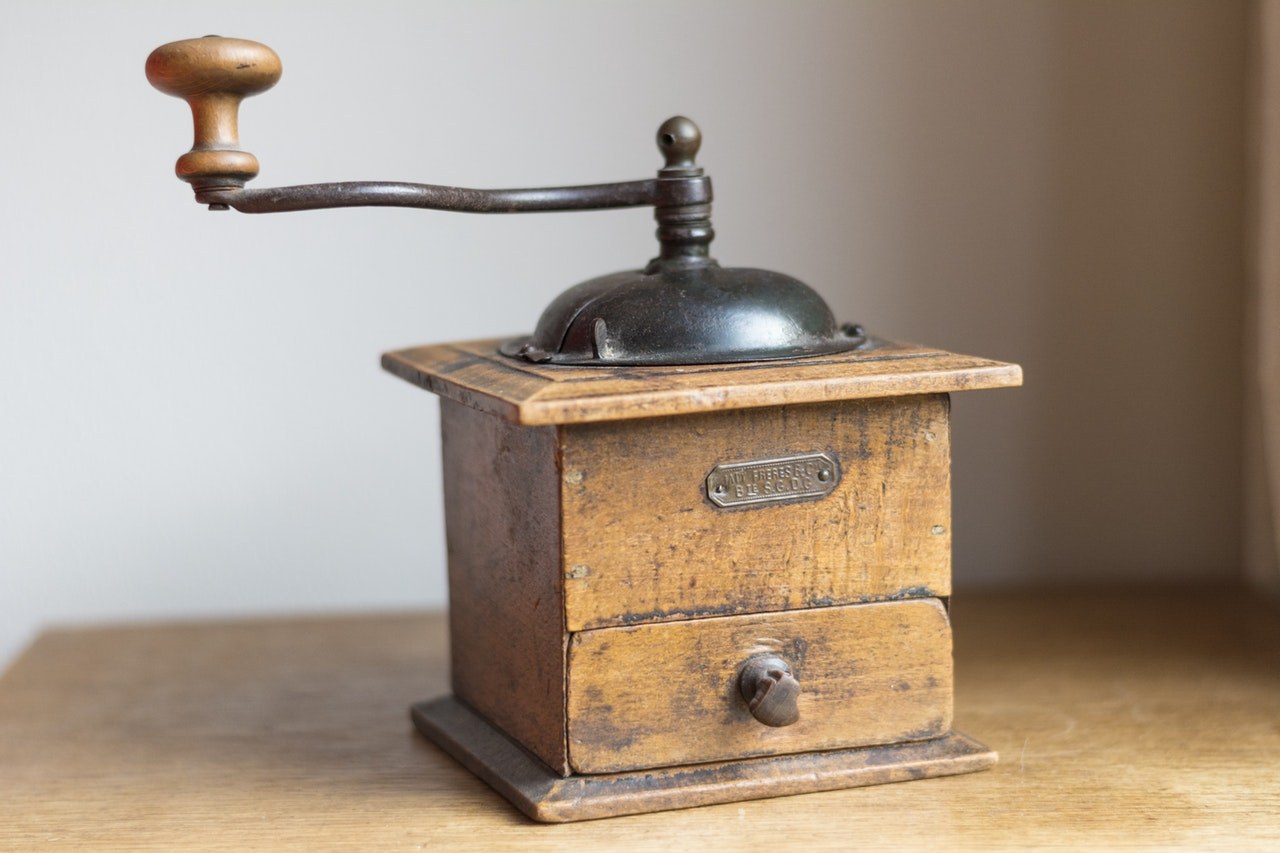
\includegraphics[width=1.0\textwidth]{../img/coffee-grinder}
\end{SlideExtra}
\fi


\begin{Slide}{Funktion: deklaration och anrop}
\SlideOnly{\setlength{\leftmargini}{0pt}}

\code{def} funktionsnamn(parameterdeklarationer): returtyp = uttryck
\vspace{0.5em}

% \begin{Code}
% def namn(param1: Typ1, param2: Typ2): Returtyp = uttryck
% \end{Code}

\begin{itemize}\SlideFontSmall
  \item En funktion har ett \Emph{huvud} och efter \code{=} kommer dess \Emph{kropp}.
  \item En \Alert{namngiven} funktion \Emph{deklareras} med nyckelordet \code{def}
  \item En funktion kan ha \Emph{parametrar} som deklareras i huvudet. 
  \item Kroppen ska vara ett uttryck (ev. ett block med flera uttryck).
  \item Parametrar binds till argument vid anrop.
  \item Uttrycket i funktionens kropp \Emph{evalueras} vid \Alert{varje anrop}. 
  \item Värdet av uttrycket blir funktionen \Emph{returvärde}. 
\end{itemize}

\pause
Exempel:
\begin{Code}
def öka(a: Int, b: Int): Int = a + b
\end{Code}
\pause
\begin{REPLnonum}
scala> öka(42, 1)
val res0: Int = 43
\end{REPLnonum}

\end{Slide}


\begin{Slide}{Deklarera funktioner, överlagring}
\begin{itemize}
\item En parameter, och sedan två parametrar:
\begin{REPL}
scala> def öka(a: Int): Int = a + 1

scala> def öka(a: Int, b: Int): Int = a + b

scala> öka(1)
val res0: Int = 2

scala> öka(1,1)
val res1: Int = 2

\end{REPL}
\item Båda funktionerna ovan kan finnas samtidigt! Trots att de har \Emph{samma namn} är de \Alert{olika funktioner}; kompilatorn kan skilja dem åt med hjälp av de \Alert{olika parameterlistorna}.

\item Detta kallas \Emph{överlagring} \Eng{overloading} av funktioner.
\item Överlagring ger flexibilitet i användningen; vi slipper hitta på nytt namn så som \code{öka2} vid 2 parametrar.
\end{itemize}
\end{Slide}



\begin{Slide}{Funktioner med defaultargument}\SlideFontSmall

\begin{itemize}
\item Vi kan ofta åstadkomma samma flexibilitet som vid överlagring, men med \Alert{en enda} funktion, om vi i stället använder \Emph{defaultargument}:
\begin{REPLnonum}
scala> def inc(a: Int, b: Int = 1) = a + b

scala> inc(42, 2)
val res0: Int = 44

scala> inc(42, 1)
val res1: Int = 43

scala> inc(42)
val res2: Int = 43

\end{REPLnonum}
\item Om ett argument utelämnas och parametern deklarerats med defaultargument så appliceras detta. Kompilatorn fyller alltså i argumentet åt oss, om det är entydigt vilken parameter som avses.
\end{itemize}
\end{Slide}


\begin{Slide}{Funktioner med namngivna argument}
\begin{itemize}
\item Genom att använda \Emph{namngivna argument} behöver man inte hålla reda på ordningen på parametrarna, bara man känner till parameternamnen.
\item Namngivna argument går fint att \Alert{kombinera} med defaultargument.
\begin{REPLnonum}[basicstyle=\SlideFontSize{7}{9}\ttfamily\color{white}]
scala> def namn(förnamn: String,
                efternamn: String,
                förnamnFörst: Boolean = true,
                ledtext: String = "Namn:"): String =
         if förnamnFörst then s"$ledtext $förnamn $efternamn"
         else s"$ledtext $efternamn, $förnamn"

scala> namn(ledtext = "Name:", efternamn = "Coder", förnamn = "Kim")
val res0: String = Name: Kim Coder
\end{REPLnonum}
\end{itemize}
\end{Slide}


\begin{Slide}{Enhetlig access}\SlideFontSmall
\begin{itemize}
\item Om en funktion \Emph{deklareras} \Alert{med} tom parameterlista \code{()} så ska den \Emph{anropas} \Alert{med} tom parameterlista.
\begin{REPLsmall}
scala> def tomParameterlista() = 42

scala> tomParameterlista()
val res1: Int = 42

scala> tomParameterlista                                                                                                                    
1 |tomParameterlista
  |^^^^^^^^^^^^^^^^^
  |method tomParameterlista must be called with () argument
\end{REPLsmall}

\item En parameterlös funktion deklarerad \Alert{utan} \code{()} ska anropas \Alert{utan} \code{()}. 
\begin{REPLsmall}
scala> def ingenParameterlista = 42
scala> ingenParameterlista()
1 |ingenParameterlista()
  |^^^^^^^^^^^^^^^^^^^
  |method ingenParameterlista does not take parameters
\end{REPLsmall}

\item Deklaration utan \code{()} möjliggör \Emph{enhetlig access}: implementationen kan ändras från \code{val} till \code{def} eller tvärtom, \Emph{utan} att \Alert{användandet} påverkas.
\pause
%\item Om parameterlista saknas får man alltså \Alert{inte} använda \code{()} vid anrop:

\end{itemize}
\end{Slide}

\Subsection{Hur ser det ut i minnet när funktioner anropas?}

\begin{Slide}{Anropsstacken och objektheapen}\SlideFontSmall
Minnet som innehåller ett programs data är uppdelat i två delar:
\begin{itemize}
\item \Emph{Anropsstacken}: 
\begin{itemize}\SlideFontSmall
\item På stackminnet läggs en \Emph{aktiveringspost} \Eng{stack frame\footnote{\href{https://en.wikipedia.org/wiki/Call_stack}{en.wikipedia.org/wiki/Call\_stack}}, activation record} för varje funktionsanrop med plats för \Alert{parametrar} och \Alert{lokala variabler}.
\item Aktiveringsposten \Alert{raderas} när \Emph{returvärdet} har levererats.
\item Stacken \Alert{växer} vid \Emph{nästlade funktionsanrop}, då en funktion i sin tur anropar en annan funktion.
\end{itemize}
\item \Emph{Objektheapen}: I heapminnet\footnote{\href{https://en.wikipedia.org/wiki/Memory_management}{en.wikipedia.org/wiki/Memory\_management}}$^{,}$\footnote{Ej att förväxlas med datastrukturen heap  \href{https://sv.wikipedia.org/wiki/Heap}{sv.wikipedia.org/wiki/Heap}} sparas alla objekt (data) som allokeras under körning. Heapen städas då och då av \Emph{skräpsamlaren} \Eng{garbage collector}, och minne som inte används längre frigörs. \\\vspace{0.5em}
%\href{http://stackoverflow.com/questions/1565388/increase-heap-size-in-java}{stackoverflow.com/questions/1565388/increase-heap-size-in-java}
% \href{https://stackoverflow.com/questions/1441373/increase-jvm-heap-size-for-scala}{stackoverflow.com/questions/1441373/increase-jvm-heap-size-for-scala}
% \begin{REPLnonum}
% scala -J-Xmx16g -J-XX:-UseGCOverheadLimit Main
% \end{REPLnonum}
\end{itemize}
\end{Slide}

% \begin{Slide}{Aktiveringspost}\SlideFontSmall
% Nästlade anrop ger växande anropsstack.
% \begin{REPL}
% scala> def f(x: Int, y: Int): Int = { val z = x + y; println(z); z}
% scala> def g(a: Int, b: Int): Int = { val c = a + b; println(c); f(c, 2 * c) }
% scala> def h(i: Int): Int = { val n = 5; g(i, i * n) }
% scala> h(2)
% \end{REPL}
%
% \pause
% \Alert{Stacken}
%
% \begin{tabular}{|r | l | l |} \hline
%
% variabel & värde & Aktiveringspost för anrop av... \\ \hline \hline
% \pause
%  i & 2 & h \\
%  n & 5 & \\ \hline
%  \pause
%  a & 2 & g \\
%  b & 10 &  \\
%  c & 12  &  \\  \hline
%  \pause
%  x & 12  & f \\
%  y & 24 &  \\
%  z & 36 & \\ \hline
% \end{tabular}
% \end{Slide}

\begin{Slide}{Aktiveringspost}\SlideFontSmall
Nästlade anrop ger växande anropsstack.
\begin{REPLsmall}
scala> def h(x: Int, y: Int) = { val z = x + y; println(z) }

scala> def g(a: Int, b: Int) = { val x = 1; h(x + 1, a + b) }

scala> def f() = { val n = 5; g(n, 2 * n) }

scala> f()

\end{REPLsmall}

\pause
\Alert{Stacken}

\begin{tabular}{|r | l | l |} \hline

variabel & värde & Aktiveringspost för anrop av... \\ \hline \hline
\pause
 n & 5 & f \\ \hline
 \pause
 a & 5 & g \\
 b & 10 &  \\
 x & 1  &  \\  \hline
 \pause
 x & 2  & h \\
 y & 15 &  \\
 z & 17 & \\ \hline
\end{tabular}
\end{Slide}

\begin{Slide}{Anropsstacken i Kojo Desktop}
Tryck på orange playknapp i Kojo och se anropsstacken.\vspace{0.5em}

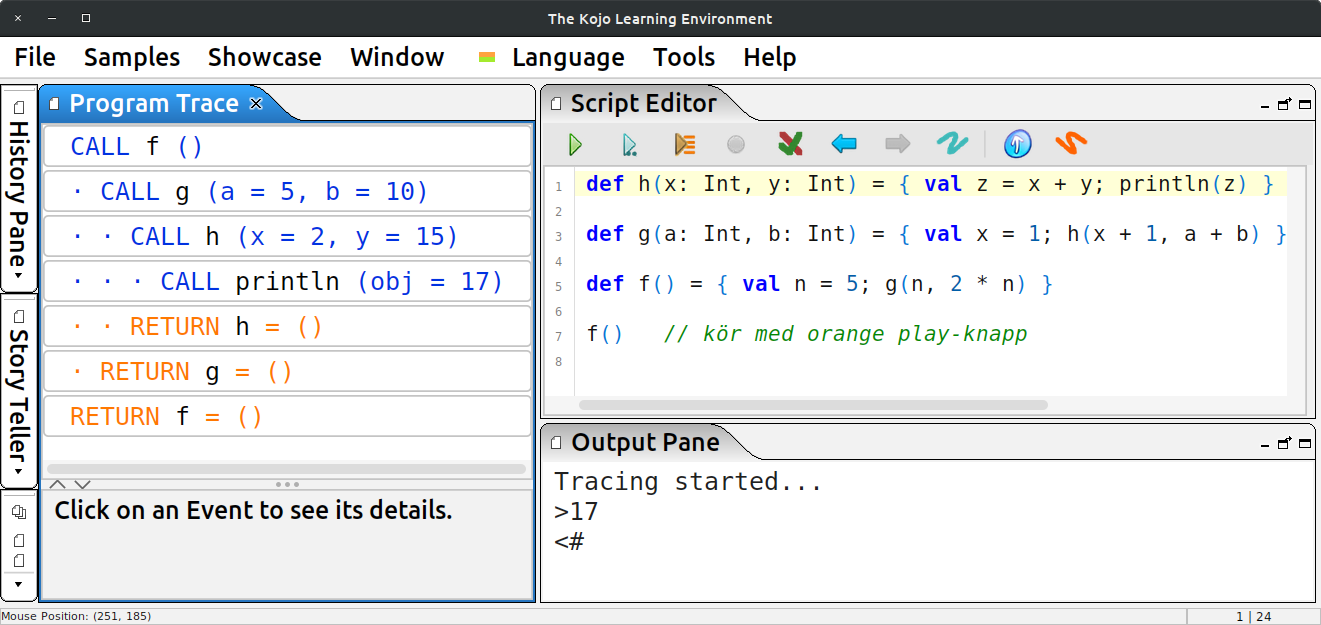
\includegraphics[width=1.0\textwidth]{../img/kojo-trace.png}  
\end{Slide}

\begin{Slide}{Anropsstacken i VS Code}
Lägg till en brytpunkt på rad 4 nedan och klicka på debug över \code{@main} i VS Code och se anropsstacken.\vspace{0.5em}

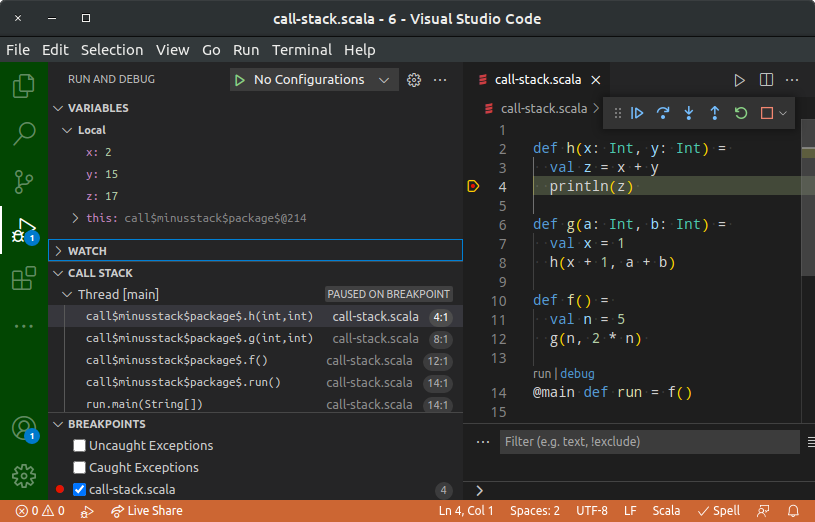
\includegraphics[width=0.85\textwidth]{../img/vscode-trace.png}  
\end{Slide}


\begin{Slide}{Vad är en stack trace?}\SlideFontSmall
När du letar buggar vid körtidsfel har du nytta av att \Alert{noga studera} \Emph{utskriften av anropsstacken} \Eng{stack trace}:
% \begin{CodeSmall}
% // Program i filen BMI.scala
% object BMI: 
%   def main(args: Array[String]): Unit = 
%     println(bmi(args(0).toInt, args(1).toInt))

%   def bmi(heightCm: Int, weightKg: Int) = 
%     safeDiv(weightKg, heightCm * heightCm) 

%   def safeDiv(numerator: Int, denominator: Int): (Int, String) = 
%     if (denominator == 0) (numerator / denominator, "ok")  // ser du buggen?
%     else (0, "division by zero") 
% \end{CodeSmall}
  
\begin{Code}[numbers=left]
// Program i filen bmi.scala

@main 
def bmi(heightCm: Int, weightKg: Int) = 
  safeDiv(weightKg, heightCm * heightCm) 

def safeDiv(numerator: Int, denominator: Int): (Int, String) = 
  if denominator == 0 then (numerator / denominator, "")  // ser du buggen?
  else (0, "division by zero")

\end{Code}
\begin{REPL}
> scalac bmi.scala 
> scala bmi 0 42
Exception in thread "main" java.lang.ArithmeticException: / by zero
        // HÄR KOMMER STACK TRACE pga körtidsfel - se nästa bild
\end{REPL}
\end{Slide}

\begin{Slide}{Hur läsa en stack trace?}
\begin{REPL}
Exception in thread "main" java.lang.ArithmeticException: / by zero
        at bmi$package$.safeDiv(bmi.scala:8)
        at bmi$package$.bmi(bmi.scala:5)
        at bmi.main(bmi.scala:3)

\end{REPL}
\begin{itemize}\SlideFontSmall
  \item En \Emph{stack trace} skrivs ut efter en krasch p.g.a. körtidsfel.
  \item Körtidsfel känns igen med ordet \Alert{Exception}.
  \item Först kommer en beskrivning av felet som orsakat kraschen, här: \\\code{java.lang.ArithmeticException: \ by zero} 
  \item Därefter visas anropsstacken.
  \item För varje funktionsanrop anges: \Emph{\texttt{klass.metod(kodfil:radnummer)}}
  \item Main-funktioner läggs i ett singelobjekt i ett speciellt paket
  \item Singelobjekt i Scala kodas som en Java-klass med dollar-tecken efter namnet, eftersom det inte finns singelobjekt i JVM.
  %\item Efter anropet av din \code{main}-procedur ligger JVM-interna anrop (\code{java.base} etc.) som du inte behöver bry dig om. %% syns inte längre i Scala 3 stack trace
\end{itemize}
\end{Slide}
  

\begin{Slide}{Lokala funktioner}\SlideFontSmall
Med lokala funktioner kan delproblem lösas med nästlade abstraktioner.

\begin{CodeSmall}
def gissaTalet(max: Int, min: Int = 1): Unit = 
  def gissat = io.StdIn.readLine(s"Gissa talet mellan $min och $max: ").toInt

  val hemlis = (math.random() * (max - min) + min).toInt

  def skrivLedtrådOmEjRätt(gissning: Int): Unit =
    if gissning > hemlis then println(s"$gissning är för stort :(")
    else if gissning < hemlis then println(s"$gissning är för litet :(")

  def inteRätt(gissning: Int): Boolean = 
    skrivLedtrådOmEjRätt(gissning)
    gissning != hemlis
  

  def loop: Int = { var i = 1; while inteRätt(gissat) do i += 1; i }

  println(s"Du hittade talet $hemlis på $loop gissningar :)")
\end{CodeSmall}

Lokala, nästlade funktionsdeklarationer är tyvärr inte tillåtna i många andra språk, t.ex. Java.\footnote{\href{http://stackoverflow.com/questions/5388584/does-java-support-inner-local-sub-methods}{\SlideFontSize{8}{9}stackoverflow.com/questions/5388584/does-java-support-inner-local-sub-methods}}

\end{Slide}

\Subsection{En funktion är ett värde}

\begin{Slide}{Funktioner är äkta värden i Scala}\SlideFontSmall
\begin{itemize}
\item En funktion är ett \Alert{äkta värde}.
\item Vi kan till exempel tilldela en variabel ett funktionsvärde.
\pause
\item Med hjälp av blank+understreck efter funktionsnamnet får vi funktionen som ett \Alert{värde} (inga argument appliceras än):
\begin{REPLnonum}
scala> def add(a: Int, b: Int) = a + b

scala> val f = add _ 
val f: (Int, Int) => Int = Lambda7210/0x0000000841e4e040@1ce2db23

scala> f(21, 21)
val res0: Int = 42
\end{REPLnonum}
\item Ett funktionsvärde har en \Alert{typ} precis som alla värden: \\
\code{f: (Int, Int) => Int}
\pause
\item Ett funktionsvärde har till skillnad från en funktionsdeklaration inget namn (variabeln \code{f} har ett namn men inte själva funktionen). Den kallas därför en \Emph{anonym} funktion eller \Alert{lambda} (mer om detta snart).
\end{itemize}
\end{Slide}

\begin{Slide}{Du kan vanligtvis skippa understreck}\SlideFontSmall
\begin{itemize}\SlideFontSmall

\item Nytt i Scala 3: Om det är otvetydigt att du vill skapa ett funktionsvärde så kan du skippa understreck:
\begin{REPLnonum}
scala> def add(a: Int, b: Int) = a + b

scala> val f = add     // inget understreck behövs 
val f: (Int, Int) => Int = Lambda7210/0x0000000841e4e040@1ce2db23
\end{REPLnonum}

\item Specialfall då understreck behövs: (se speciellt typen \code{() => Int})
\begin{REPLsmall}
scala> def a() = 42
def a(): Int

scala> val b = a
1 |val b = a
  |        ^
  |        method a must be called with () argument

scala> val b = a _
val b: () => Int = Lambda7214/0x0000000841e50440@565d794
\end{REPLsmall}
\item Börja utan understreck och se om det funkar utan kompileringsfel...
\end{itemize}
\end{Slide}

\begin{Slide}{Funktionsvärden kan vara argument}
En funktion kan ha en annan funktion som parameter:
\begin{REPL}
scala> def tvåGånger(x: Int, f: Int => Int) = f(f(x))

scala> def öka(x: Int) = x + 1

scala> def minska(x: Int) = x - 1

scala> tvåGånger(42, öka)
val res1: Int = 44

scala> tvåGånger(42, minska)
val res1: Int = 40
\end{REPL}
\end{Slide}



\begin{Slide}{Applicera funktioner på element i samlingar med \texttt{map}}\SlideFontSmall
\begin{Code}
def öka(x: Int) = x + 1

def minska(x: Int) = x - 1

val xs = Vector(1, 2, 3)
\end{Code}
\pause
Metoden \Emph{\texttt{map}} fungerar på alla Scala-samlingar och tar \Emph{en funktion som argument} och applicerar denna funktion på alla element och \Alert{skapar en ny samling} med resultaten:
\begin{REPL}
scala> xs.map(öka)
val res0: ???   // vad blir resultatet?

scala> xs.map(minska)
val res1: ???   // vad blir resultatet?
\end{REPL}
En funktion som har funktionsvärden som indata (eller utdata) kallas en\\ \Emph{högre ordningens funktion}  \Eng{higher-order function}.
\end{Slide}


\begin{Slide}{Applicera funktioner på element i samlingar med \texttt{map}}\SlideFontSmall
\begin{Code}
def öka(x: Int) = x + 1

def minska(x: Int) = x - 1

val xs = Vector(1, 2, 3)
\end{Code}
Metoden \Emph{\texttt{map}} fungerar på alla Scala-samlingar och tar \Emph{en funktion som argument} och applicerar denna funktion på alla element och \Alert{skapar en ny samling} med resultaten:
\begin{REPL}
scala> xs.map(öka)
val res0: scala.collection.immutable.Vector[Int] = Vector(2, 3, 4)

scala> xs.map(minska)
val res1: scala.collection.immutable.Vector[Int] = Vector(0, 1, 2)
\end{REPL}
En funktion som har funktionsvärden som indata kallas en\\ \Emph{högre ordningens funktion}  \Eng{higher-order function}.
\end{Slide}

\Subsection{Äkta funktioner}

\begin{Slide}{Äkta funktioner}
\begin{itemize}\SlideFontSmall
\item En \Emph{äkta} \Eng{pure} funktion är en funktion som ger ett resultat som \Alert{enbart} beror av dess argument. Alltså som funktioner i matematiken.
\item En äkta (matematisk) funktion är \Emph{referentiellt transparent} \Eng{referentially transparent}, vilket innebär att varje anrop kan bytas ut mot funktionskroppen där parametrarna ersatts med motsvarande argument.
\item En äkta funktion har \Alert{inga sidoeffekter}, t.ex. utskrift, skriva/läsa filer,  eller uppdateringar av variabler \Alert{synliga utanför} funktionen.
\item Exempel:
\begin{Code}
def add(x: Int, y: Int): Int = x + y              // äkta funktion
def rnd(n: Int): Int = (math.random() * n).toInt  // oäkta funktion
\end{Code} 
\begin{itemize}\SlideFontTiny

\item Uttrycket \code{add(41, 1)} kan ersättas med 41 +1 som i sin tur kan ersättas med 42 utan att det påverkar resultatet. Resultatet av \code{add(41, 1)} blir \Emph{samma varje gång} funktionen appliceras med dessa argument
\item Uttrycket \code{rnd(42)} kan \Alert{inte} bytas ut mot ett specifikt uttryck som säkert ger samma resultat varje gång. Alltså: \emph{ej referentiell transparens}.
\end{itemize}  
\end{itemize}  
\end{Slide}

\begin{Slide}{Exempel på oäkta funktioner: slumptal}

  \begin{itemize}
    \item Funktioner vars värden på något sätt beror av slumpen är \Alert{inte} äkta funktioner.
    \item Även om samma argument ges vid upprepad applicering, så kan ju resultatet bli olika.
    \item Studera dokumentationen för \code{scala.util.Random} här:\\ \href{https://www.scala-lang.org/api/current/scala/util/Random.html}{\SlideFontSmall https://www.scala-lang.org/api/current/scala/util/Random.html}
    \item Du har nytta av funktionen \code{Random.nextInt} och slumptalsfrö \Eng{random seed} i veckans uppgifter.
  \end{itemize}

\end{Slide}

\begin{Slide}{Slumptalsfrö: få samma slumptal varje gång}\SlideFontTiny
\begin{itemize}
\item Om man använder slumptal kan det vara svårt att leta buggar, efter som det blir \Alert{olika varje gång} man kör programmet och buggen kanske bara uppstår ibland.

\item Med klassen \code{scala.util.Random} kan man skapa \Emph{pseudo}-slumptalssekvenser.
\pause
\item Om man ger ett s.k. \Emph{frö} \Eng{seed}, av heltalstyp, som argument till konstruktorn när man skapar en instans av klassen \code{scala.util.Random}, får man samma ''slumpmässiga'' sekvens \Alert{varje gång} man kör programmet.

\begin{Code}
  val seed = 42
  val rnd = util.Random(seed) // skapa ny slumpgenerator med frö 42
  val r = rnd.nextInt(6) // ger slumptal mellan 0 till och med 5
\end{Code}
\pause
\item Om man \Alert{inte} ger ett \Emph{frö} så sätts fröet till ''\emph{a value very likely to be distinct from any other invocation of this constructor}''. Då vet vi inte vilket fröet blir och det blir olika varje gång man kör programmet.
\begin{Code}
  val rnd = util.Random() // OLIKA frö varje körning
  val r = rnd.nextInt(6) // ger slumptal mellan 0 till och med 5
\end{Code}
\pause
\end{itemize}
\end{Slide}

%\begin{Slide}{Syresättning av hjärnan vid sövande föreläsning}
%Prova nedan kod som finns här:\\
%%\href{https://github.com/lunduniversity/introprog/blob/master/compendium/examples/workspace/w05-seqalg/src/NanananananananaNanananananananaBatman.scala}{\SlideFontTiny github.com/lunduniversity/introprog/.../NanananananananaNanananananananaBatman.scala} \\
%
%
%
%\vspace{0.65em}\scalainputlisting[numbers=left,numberstyle=,basicstyle=\fontsize{6.5}{8}\ttfamily\selectfont]{../compendium/examples/workspace/w05-seqalg/src/FixSleepyBrain.scala}
%
%\pause
%Medan du lyssnar till: \href{https://www.youtube.com/watch?v=zUwEIt9ez7M}{\SlideFontSmall www.youtube.com/watch?v=zUwEIt9ez7M}\\
%Eller: \href{https://www.youtube.com/watch?v=rvXxlXg_V-k}{\SlideFontSmall www.youtube.com/watch?v=rvXxlXg\_V-k}
%\end{Slide}

\Subsection{Anonyma funktioner}


\begin{Slide}{Anonyma funktioner}
\begin{itemize}
\item  Man behöver inte ge funktioner namn. De kan i stället skapas med hjälp av \Emph{funktionsliteraler}.\footnote{Även kallat ''lambda-värde'' eller bara ''lambda'' efter den s.k. lambdakalkylen. \href{https://en.wikipedia.org/wiki/Anonymous_function}{en.wikipedia.org/wiki/Anonymous\_function}}

\item En funktionsliteral har ...
\begin{enumerate}
\item en parameterlista (utan funktionsnamn, utan returtyp),
\item sedan den reserverade teckenkombinationen \code{=>}
\item och sedan ett uttryck (eller ett block).
\end{enumerate}
\pause
\item Exempel:
\begin{Code}[basicstyle=\ttfamily\SlideFontSize{9}{11}]
(x: Int, y: Int) => x + y             // vilken typ?
\end{Code}
\pause
\item Om kompilatorn kan gissa typerna från sammanhanget så behöver typerna inte anges i själva  funktionsliteralen:
\begin{Code}[basicstyle=\ttfamily\SlideFontSize{9}{11}]
val f: (Int, Int) => Int = (x, y) => x + y
\end{Code}
\end{itemize}
\end{Slide}


\begin{Slide}{Applicera anonyma funktioner på element i samlingar}\SlideFontSmall
Anonym funktion skapad med funktionsliteral direkt i anropet:
\begin{REPL}
scala> val xs = Vector(1, 2, 3)

scala> xs.map((x: Int) => x + 1)
res0: scala.collection.immutable.Vector[Int] = Vector(2, 3, 4)
\end{REPL}
\pause
Eftersom kompilatorn här kan härleda typerna så behövs de inte:
\begin{REPL}
scala> xs.map(x => x + 1)
res1: scala.collection.immutable.Vector[Int] = Vector(2, 3, 4)
\end{REPL}
\pause
Om man bara använder parametern en enda gång i funktionen så kan man byta ut parameternamnet mot ett understreck.
\begin{REPL}
scala> xs.map(_ + 1)
res2: scala.collection.immutable.Vector[Int] = Vector(2, 3, 4)
\end{REPL}
\end{Slide}



\begin{Slide}{Platshållarsyntax för anonyma funktioner}\SlideFontSmall
Understreck i funktionsliteraler kallas \Emph{platshållare} \Eng{placeholder} och medger ett förkortat skrivsätt \Alert{om} den parameter som understrecket representerar används \Alert{endast en gång}.
\begin{Code}[basicstyle=\ttfamily\fontsize{10}{12}\selectfont]
_ + 1
\end{Code}
Ovan expanderas av kompilatorn till följande funktionsliteral \\(där namnet på parametern är godtyckligt):
\begin{Code}[basicstyle=\ttfamily\fontsize{10}{12}\selectfont]
x => x + 1
\end{Code}
\pause
Det kan förekomma flera understreck; det första avser första parametern, det andra avser andra parametern etc.
\begin{Code}[basicstyle=\ttfamily\fontsize{10}{12}\selectfont]
_ + _
\end{Code}
\pause
... expanderas till:
\begin{Code}[basicstyle=\ttfamily\fontsize{10}{12}\selectfont]
(x, y) => x + y
\end{Code}
\end{Slide}


\begin{Slide}{Exempel på platshållarsyntax med \texttt{reduceLeft}}\SlideFontSmall
Metoden \code{reduceLeft} applicerar en funktion på de två första elementen i en sekvens och tar sedan resultatet som första argument och nästa element som andra argument och upprepar detta genom hela samlingen.
\begin{REPL}
scala> def summa(x: Int, y: Int) = x + y

scala> val xs = Vector(1, 2, 3, 4, 5)

scala> xs.reduceLeft(summa)
res20: Int = 15

scala> xs.reduceLeft((x, y) => x + y)
res21: Int = 15

scala> xs.reduceLeft(_ + _)
res22: Int = 15

scala> xs.reduceLeft(_ * _)
res23: Int = 120
\end{REPL}
\end{Slide}


\begin{Slide}{Predikat, med och utan namn}
\begin{itemize}\SlideFontSmall
\item En funktion som har \code{Boolean} som returtyp kallas för ett \Emph{predikat}. 
\item Exempel:
\begin{Code}
def isTooLong(name: String): Boolean = name.length > 10

def isTall(heightInMeters: Double, limit: Double = 1.78): Boolean = 
  heightInMeters > limit
\end{Code}
\item Predikat ges ofta ett namn som börjar på \code{is} eller \code{has} så att man lätt kan se att det är ett predikat när man läser kod som anropar funktionen.
\item Många av samlingsmetoderna i Scalas standardbibliotek tar predikat som funktionsargument. Exempel med predikat som anonym funktion: 
\begin{REPLnonum}
scala> val parts = Vector(3, 1, 0, 5).partition(_ > 1)
val parts: (Vector[Int], Vector[Int]) = 
  (Vector(3, 5),Vector(1, 0))
\end{REPLnonum} 
\item Studera snabbreferensen och försök hitta samlingsmetoder som tar predikat som funktionsargument. \url{http://cs.lth.se/pgk/quickref} \\I anropsexempel med predikat-argument används bokstaven \code{p}.
\end{itemize}  
\end{Slide}


\Subsection{Skapa din egen kontrollstruktur}  

\begin{Slide}{Hur fungerar egentligen \code{upprepa} i Kojo?}
\begin{Code}[basicstyle=\ttfamily\SlideFontSize{14}{16}]
upprepa(10) {
  println("hej")
}
\end{Code}

\pause
Vi ska nu se hur vi, genom att kombinera ett antal koncept, kan skapa egna kontrollstrukturer likt upprepa ovan:
\begin{itemize}
\item klammerparentes vid ensam paramenter
\item multipla parameterlistor
\item namnanrop (fördröjd evaluering)
\end{itemize}
\end{Slide}



\begin{Slide}{Multipla parameterlistor}
Vi har tidigare sett att man kan ha mer än en parameter:
\begin{REPLnonum}
scala> def add(a: Int, b: Int) = a + b

scala> add(21, 21)
res0: Int = 42
\end{REPLnonum}
Man kan även ha \Alert{mer än en} \Emph{parameterlista}:
\begin{REPLnonum}
scala> def add(a: Int)(b: Int) = a + b

scala> add(21)(21)
res1: Int = 42
\end{REPLnonum}
\Eng{multiple parameter lists}

\href{http://docs.scala-lang.org/style/declarations.html#multiple-parameter-lists}{\SlideFontTiny docs.scala-lang.org/style/declarations.html\#multiple-parameter-lists}
\end{Slide}



\begin{Slide}{Värdeanrop och namnanrop}\SlideFontSmall
Det vi sett hittills är \Emph{värdeanrop}: argumentet evalueras \Alert{först} innan dess \Alert{värde} \emph{sedan} appliceras:
\begin{REPL}
scala> def byValue(n: Int): Unit = for i <- 1 to n do print(" " + n)

scala> byValue(21 + 21)
 42 42 42 42 42 42 42 42 42 42 42 42 42 42 42 42 42 42 42 42 42 42 42 42 42 42 42 42 42 42 42 42 42 42 42 42 42 42 42 42 42 42

scala> byValue({print(" hej"); 21 + 21})
 hej 42 42 42 42 42 42 42 42 42 42 42 42 42 42 42 42 42 42 42 42 42 42 42 42 42 42 42 42 42 42 42 42 42 42 42 42 42 42 42 42 42 42
\end{REPL}
\pause
Men man kan med \code{=>} före parametertypen åstadkomma \Emph{namnanrop}: argumentet \Alert{''klistras in''} i stället för \Alert{namnet} och evalueras \Alert{varje gång} (kallas även \Emph{fördröjd evaluering}):
\begin{REPL}
scala> def byName(n: => Int): Unit = for i <- 1 to n do print(" " + n)

scala> byName({print(" hej"); 21 + 21})
 hej hej 42 hej 42 hej 42 hej 42 hej 42 hej 42 hej 42 hej 42 hej 42 hej 42 hej 42 hej 42 hej 42 hej 42 hej 42 hej 42 hej 42 hej 42 hej 42 hej 42 hej 42 hej 42 hej 42 hej 42 hej 42 hej 42 hej 42 hej 42 hej 42 hej 42 hej 42 hej 42 hej 42 hej 42 hej 42 hej 42 hej 42 hej 42 hej 42 hej 42 hej 42 hej 42
\end{REPL}
\Alert{Kluring}: Varför skrivs ''hej'' ut en extra gång i början? \pause ledtråd: \texttt{1 to \Alert{n}}
%evalueringen av n i 1 to n ger ett extra hej
\end{Slide}

\begin{Slide}{Klammerparenteser vid ensam parameter}
Så här har vi sett nyss att man man göra:
\begin{REPL}
scala> def twice(action: => Unit): Unit = { action; action }

scala> twice( { print("hej"); print("san ") } )
hejsan hejsan
\end{REPL}

Det ser rätt klyddigt ut med \code+{(+  och \code+)}+ eller vad tycker du? \pause Men...
För alla funktioner \code{f} gäller att: \\ det är helt ok att byta ut vanliga parenteser: \hfill\code{f(uttryck)} \\ mot krullparenteser: \hfill\code|f{uttryck}| \\ \Alert{om} parameterlistan har \Alert{exakt en} parameter.

\vspace{0.5em}Man kan alltså skippa det yttre parentesparet för bättre läsbarhet:
\begin{REPLnonum}
scala> twice { print("hej"); print("san ") }
\end{REPLnonum}
\end{Slide}



\begin{Slide}{Skapa din egen kontrollstruktur}
\begin{itemize}
\item Genom att \Alert{kombinera} \Emph{multipla parameterlistor} med \Emph{namnanrop} med \Emph{klammerparentes vid ensam parameter} kan vi skapa vår egen kontrollstruktur: \code{upprepa} \pause
\begin{Code}
upprepa(42){
  if math.random() < 0.5 then print(" gurka")
  else print(" tomat")
}
\end{Code}
Hur då?
\pause
 Till exempel så här:
\begin{Code}
def upprepa(n: Int)(block: => Unit) = 
  for i <- 0 until n do block
\end{Code}

\pause

\begin{REPLnonum}
gurka gurka gurka tomat tomat gurka gurka gurka gurka tomat tomat tomat tomat tomat
\end{REPLnonum}
\end{itemize}
\end{Slide}


\begin{Slide}{Stegade funktioner, ''Curry-funktioner''}
Om en funktion har multipla parameterlistor kan man skapa \Emph{stegade funktioner}, även kallat \Emph{partiellt applicerade} funktioner \Eng{partially applied functions} eller \Emph{''Curry''-funktioner}.
\begin{REPLnonum}
scala> def add(x: Int)(y: Int) = x + y

scala> val öka = add(1)
val öka: Int => Int = Lambda7339/0x0000000841eb7040@19c8add7

scala> Vector(1,2,3).map(öka)
val res0: Vector[Int] = Vector(2, 3, 4)

scala> Vector(1,2,3).map(add(2))
val res1: Vector[Int] = Vector(3, 4, 5)
\end{REPLnonum}
\end{Slide}


\begin{Slide}{Funktion med fångad variabelrymd: \textit{closure}}
\begin{Code}
def f(x: Int): Int => Int = 
  val a = 42 + x
  def g(y: Int): Int = y + a
  g
\end{Code}
Funktionen \code{g} \Alert{fångar} den lokala variabeln \code{a} i ett \Emph{funktionsobjekt}.
\pause
\begin{REPLnonum}
scala> val funkis = f(1)
val funkis: Int => Int = Lambda7356/0x0000000841ed2840@1bda26bc

scala> funkis(2)
val res0: Int = 45
\end{REPLnonum}
\pause
Ett funktionsobjekt med ''fångade'' variabler kallas \Alert{closure}. \\
(Mer om funktioner som objekt senare.)
\end{Slide}

\ifkompendium\else
\begin{SlideExtra}{Översikt av begrepp vi gått igenom hittills}
\begin{enumerate}
\item överlagring
\item utelämna tom parameterlista (enhetlig access)
\item defaultargument
\item namngivna argument
\item lokala funktioner
\item funktioner som äkta värden
\item anonyma funktioner
\item klammerparentes vid ensam paramenter
\item multipla parameterlistor
\item namnanrop (fördröjd evaluering)
\item egendefinierade kontrollstrukturer
\item stegade funktioner (''Curry-funktioner'')
\item fångad variablelrymd i funktionsobjekt (''closure'')
\end{enumerate}
\end{SlideExtra}
\fi



\Subsection{Kort om rekursion}

\begin{Slide}{Rekursiva funktioner}
\begin{itemize}
\item Funktioner som \Alert{anropar sig själv} kallas \Emph{rekursiva}.


\begin{REPLnonum}
scala> def fakultet(n: Int): Int =
         if n < 2 then 1 else n * fakultet(n - 1)

scala> fakultet(5)
val res0: Int = 120
\end{REPLnonum}

\item För varje nytt anrop läggs en ny aktiveringspost på stacken.

\item I aktiveringsposten sparas varje returvärde som gör att \code{5 * (4 * (3 * (2 * 1)))} kan beräknas.

\item Rekrusionen avbryts när man når \Emph{basfallet}, här \code{n < 2}

\item En rekursiv funktion \Alert{måste} ha en returtyp.

\end{itemize}

\end{Slide}

\begin{Slide}{Loopa med rekursion}
\begin{Code}
def gissaTalet(max: Int, min: Int = 1): Unit =
  def gissat = 
    io.StdIn.readLine(s"Gissa talet mellan [$min, $max]: ").toInt

  val hemlis = (math.random() * (max - min) + min).toInt

  def skrivLedtrådOmEjRätt(gissning: Int): Unit =
    if gissning > hemlis then println(s"$gissning är för stort :(")
    else if (gissning < hemlis) println(s"$gissning är för litet :(")

  def ärRätt(gissning: Int): Boolean = 
    skrivLedtrådOmEjRätt(gissning)
    gissning == hemlis

  def loop(n: Int = 1): Int = if ärRätt(gissat) then n else loop(n + 1)

  println(s"Du hittade talet $hemlis på ${loop()} gissningar :)")
\end{Code}
\end{Slide}


\begin{Slide}{Rekursiva datastrukturer}
\begin{itemize}
\item Datastrukturena Lista och Träd är exempel på datastrukturer som passar bra ihop med rekursion.
\item Båda dessa datastrukturer kan beskrivas rekursivt:
\begin{itemize}
\item En lista består av ett huvud och en lista, som i sin tur består av ett huvud och en lista, som i sin tur...
\item Ett träd består av grenar till träd som i sin tur består av grenar till träd som i sin tur, ...
\end{itemize}
\item Dessa datastrukturer bearbetas med fördel med rekursiva algoritmer.
\item I denna kursen ingår rekursion endast ''för kännedom'': \\ du ska veta vad det är och kunna skapa en enkel rekursiv funktion, t.ex. fakultets-beräkning. Du kommer jobba mer med rekursion och rekursiva datastrukturer i fortsättningskursen.
\end{itemize}
\end{Slide}

\Subsection{Automatisera kompilering: byggverktyg}

\begin{Slide}{Bygga applikationer}
\begin{itemize}
  \item Den kreativa programmeringsprocessen innehåller många korta cykler av koda, ändra, testa.
  \item Det blir många omkompileringar och då vill man gärna slippa skriva samma kommando om och om igen. En lösning är att skapa ett skript, t.ex. i språket \Emph{bash}, som kör kompileringen.
  \item  Om man bara gör en liten ändring vill man bara kompilera om det som ändrats och inte kompilera om rubbet varje gång. En lösning på detta problem är att använda ett \Emph{byggverktyg}, t.ex. Scala Build Tool (\code{sbt}), se Appendix F.

\end{itemize}
\end{Slide}

\begin{Slide}{Bash-skript för kompilering}\SlideFontSmall
\begin{itemize}
  \item Det gamla skriptspråket \Emph{bash} funkar i Linux och MacOS.
  \item Bash är smidigt för enkla program som använder terminalkommando, men syntaxen är knepig och det finns många fallgropar.
  \item I ett bash-skript kan du t.ex. kompilera och köra ett program. Exempel i filen \code{build.sh} nedan:
\begin{Code}
scalac mitt-program.scala && scala MinMain
\end{Code}
Med pil-upp kan du enkelt kompilera om efter varje ändring:
\begin{REPLnonum}
> sh build.sh
\end{REPLnonum}
  \item Det går att få \Emph{bash} och ubuntu-terminalen att funka i Windows 10 med WSL (Windows Linux Subsystem) där du kan välja Ubuntu 18.04 LTS: \\
  {\SlideFontTiny\url{https://docs.microsoft.com/en-us/windows/wsl/install-win10}}
\end{itemize}
{\noindent   Det finns dock stora begränsningar med WSL och om du vill ha Linux ''på riktigt'' rekommenderas att du installera Ubuntu med dual-boot: \SlideFontTiny\url{https://linoxide.com/distros/install-ubuntu-18-04-dual-boot-windows-10/}}
\end{Slide}

\begin{Slide}{Scala Build Tool: \texttt{sbt}}
\begin{itemize}
  \item Ett byggverktyg, t.ex. \code{sbt}, kan användas för att kompilera, testköra, ladda ner, paketer, distribuera programbibliotek och applikationer.
  \item Det är mycket enkelt att använda \code{sbt} för att kompilera och köra om ditt program varje gång du sparar din fil, tex. med \code{Ctrl+S} så här:
\begin{REPLnonum}
> sbt
sbt> ~run   // tecknet ~ ger omkörning vid ändring
\end{REPLnonum}
Tecknet \code{~} kallas \emph{tilde} och skrivs med högra Alt-tangenten nere och två tryck på tangenten bredvid Enter.
  \item LTH:s datorer har \code{sbt} förinstallerat. Ladda ner till din dator: \\
  \url{https://www.scala-sbt.org/download.html}
  \item Läs mer om byggverktyg i Appendix F.

\end{itemize}

\end{Slide}




\ifkompendium\else
\Subsection{Veckans uppgifter}

\begin{SlideExtra}{Mål med övning \ExeWeekTHREE}
\begin{itemize}\SlideFontSmall
  %!TEX encoding = UTF-8 Unicode
%!TEX root = ../exercises.tex

\item Kunna skapa och använda funktioner med en eller flera parametrar, default-argument, och namngivna argument.
\item Kunna förklara nästlade funktionsanrop med aktiveringsposter på stacken.
\item Kunna förklara skillnaden mellan äkta och ''oäkta'' funktioner.
\item Kunna applicera en funktion på alla element i en samling.

\item Kunna använda funktioner som äkta värden.
\item Kunna skapa och använda anonyma funktioner (ä.k. lambda-funktioner).

\item Känna till att funktioner kan ha uppdelad parameterlista.
\item Känna till att det går att partiellt applicera argument på funktioner med uppdelad parameterlista för att skapa s.k. stegade funktioner (ä.k. curry-funktioner).

\item Känna till rekursion och kunna beskriva vad som kännetecknar en rekursiv funktion.
%\item Känna till att man kan loopa med rekursion och att svansrekursiva funktioner kan optimeras till while-loopar.

\item Känna till att det går att skapa egna kontrollstrukturer med hjälp av namnanrop.
\item Känna till skillnaden mellan värdeanrop och namnanrop.
\item Kunna tolka en stack trace.

\end{itemize}
\end{SlideExtra}

\begin{SlideExtra}{Mål med laboration \LabWeekTHREE}
\begin{itemize}
  %!TEX encoding = UTF-8 Unicode
%!TEX root = ../compendium2.tex

%\item Kunna kompilera Scalaprogram med \texttt{scalac}.
%\item Kunna köra Scalaprogram med \texttt{scala}.
%\item Kunna definiera och anropa funktioner.
%\item Kunna använda och förstå default-argument.
%\item Kunna ange argument med parameternamn.
\item Kunna skapa ett större program med din egen kod efter dina egna idéer.
\item Kunna använda en editor och terminalen för att iterativt editera, kompilera, och testa din kod.
\item Kunna använda variabler i kombination med alternativ och repetetition i flera nivåer.
\item Kunna stegvis förbättra din kod för att underlätta förändring och öka läsbarhet.
\item Kunna skapa och använda abstraktioner för att generalisera och möjliggöra återanvändning av kod.

\end{itemize}
Ni ska spela \Emph{varandras} textspel i din \Alert{samarbetsgrupp}.\\
Läs labbinstruktioner:\url{http://cs.lth.se/pgk/compendium/}
\end{SlideExtra}


\begin{SlideExtra}{Tips till ditt textspel.}
\begin{CodeSmall}
"Yes".toLowerCase.startsWith("y")    // true
"hejsan".contains("ejsa")            // true
"42".toInt                           // 42
"?".toIntOption.getOrElse(42)        // 42
Thread.sleep(1000)                   // ger lagom irriterande fördröjning (1 sekund)

val i = 42
s"Livets mening är $i!" // dollar $ före namn vid stränginterpolering med s""
s"Livets mening är inte ${i-1}!"  // klamrar ${} vid evaluering av uttryck

"""|en sträng som spänner över
   |flera rader där marginalen fram till vertikalstreck
   |är bortplockad med stripMargin (kan kombineras med s-interpolatorn)
""".stripMargin

math.random() < 0.8                  // true i 80% av fallen
scala.util.Random.nextInt(42)      // ger slumptal mellan 0 och 41
scala.io.StdIn.readLine("prompt>") // ger sträng som användaren skriver

val x = try { "?".toInt } catch { case e: Exception => 42 }  // förhindrar krasch
Thread.sleep(1000)    // sova i 1000 milliskeunder
\end{CodeSmall}
Kolla \Emph{snabbreferensen} vad mer du kan göra med strängar!
\end{SlideExtra}

\begin{SlideExtra}{Exempel på en början till ett textspel}
  Här finns en exempel på en enkel \emph{början} på ett textspel som du stegvis kan ändra och bygga ut till något du själv vill göra:
  \url{https://github.com/lunduniversity/introprog/tree/master/workspace/w03_irritext}

\begin{itemize}
  \item Vilka begrepp och principer ger koden träning i?
\end{itemize}

\end{SlideExtra}

\begin{SlideExtra}{Jobba så här}
\begin{itemize}
  \item Skriv koden i en editor.
  \item Ha ett terminalfönster med \code{sbt} där du kör \code{~compile} eller \code{~run} så att din kod kompileras eller körs om varje gång du sparar.
  \item Ha ett terminalfönster med en fristående scala REPL där du kan göra mindre undersökningar rad för rad.
  \item Börja enkelt och bygg vidare steg för steg.
  \item Bygg om koden allteftersom den växer genom att införa nya abstraktioner med väl valda namn (s.k. ''refaktorisering'') .
  \item Fixa \Alert{alla} kompileringsfel \code{||} körtidsfel \Emph{innan} du går vidare.
  \item Fokusera på kodens \Alert{läsbarhet}.
\end{itemize}

\end{SlideExtra}

\fi


%\chapter{Funktioner, Objekt}\label{chapter:W03}
Koncept du ska lära dig denna vecka:
\begin{multicols}{2}\begin{itemize}[nosep,label={$\square$},leftmargin=*]
\item definera funktion
\item anropa funktion
\item parameter
\item returtyp
\item värdeandrop
\item namnanrop
\item default-argument
\item namngivna argument
\item applicera funktion på alla element i en samling
\item procedur
\item värdeanrop vs namnanrop
\item uppdelad parameterlista
\item skapa egen kontrollstruktur
\item objekt
\item modul
\item punktnotation
\item tillstånd
\item metod
\item medlem
\item funktionsvärde
\item funktionstyp
\item äkta funktion
\item stegad funktion
\item apply
\item lazy val
\item lokala funktioner
\item aktiveringspost
\item rekursion
\item basfall
\item anropsstacken
\item objektheapen
\item cslib.window.SimpleWindow\end{itemize}\end{multicols}

%!TEX encoding = UTF-8 Unicode
%!TEX root = ../exercises.tex

\ifPreSolution

\Exercise{\ExeWeekTHREE}\label{exe:W03}
\begin{Goals}
%!TEX encoding = UTF-8 Unicode
%!TEX root = ../exercises.tex

\item Kunna skapa och använda funktioner med en eller flera parametrar, default-argument, och namngivna argument.
\item Kunna förklara nästlade funktionsanrop med aktiveringsposter på stacken.
\item Kunna förklara skillnaden mellan äkta och ''oäkta'' funktioner.
\item Kunna applicera en funktion på alla element i en samling.

\item Kunna använda funktioner som äkta värden.
\item Kunna skapa och använda anonyma funktioner (ä.k. lambda-funktioner).

\item Känna till att funktioner kan ha uppdelad parameterlista.
\item Känna till att det går att partiellt applicera argument på funktioner med uppdelad parameterlista för att skapa s.k. stegade funktioner (ä.k. curry-funktioner).

\item Känna till rekursion och kunna beskriva vad som kännetecknar en rekursiv funktion.
%\item Känna till att man kan loopa med rekursion och att svansrekursiva funktioner kan optimeras till while-loopar.

\item Känna till att det går att skapa egna kontrollstrukturer med hjälp av namnanrop.
\item Känna till skillnaden mellan värdeanrop och namnanrop.
\item Kunna tolka en stack trace.

\end{Goals}

\begin{Preparations}
\item \StudyTheory{03}
\end{Preparations}

\BasicTasks %%%%%%%%%%%%%%%%

\else

\ExerciseSolution{\ExeWeekTHREE}

\fi





\WHAT{Para ihop begrepp med beskrivning.}

\QUESTBEGIN

\Task \what

\vspace{1em}\noindent Koppla varje begrepp med den (förenklade) beskrivning som passar bäst:

\begin{ConceptConnections}
  funktionshuvud & 1 & & A & fördröjd evaluering av argument \\ 
  funktionskropp & 2 & & B & koden som exekveras vid funktionsanrop \\ 
  parameterlista & 3 & & C & funktion utan namn; kallas även lambda \\ 
  block & 4 & & D & gör att argument kan ges i valfri ordning \\ 
  namngivna argument & 5 & & E & en funktion som anropar sig själv \\ 
  defaultargument & 6 & & F & gör att en funktion kan flera resultatvärden \\ 
  värdeanrop & 7 & & G & har parameterlista och eventuellt returtyp \\ 
  namnanrop & 8 & & H & kan ha lokala namn; sista raden ger värdet \\ 
  tupel & 9 & & I & lista med bestämt antal (heterogena) värden \\ 
  tupelreturtyp & 10 & & J & argumentet evalueras innan anrop \\ 
  äkta funktion & 11 & & K & ger alltid samma resultat om samma argument \\ 
  slumptalsfrö & 12 & & L & beskriver namn och typ på parametrar \\ 
  anonym funktion & 13 & & M & gör att argument kan utelämnas \\ 
  rekursiv funktion & 14 & & N & om lika blir sekvensen av pseudoslumptal samma \\ 
\end{ConceptConnections}

\SOLUTION

\TaskSolved \what

\begin{ConceptConnections}
  funktionshuvud & 1 & ~~\Large$\leadsto$~~ &  M & har parameterlista och eventuellt en returtyp \\ 
  funktionskropp & 2 & ~~\Large$\leadsto$~~ &  L & koden som exekveras vid funktionsanrop \\ 
  parameterlista & 3 & ~~\Large$\leadsto$~~ &  I & beskriver namn och typ på parametrar \\ 
  block & 4 & ~~\Large$\leadsto$~~ &  E & kan ha lokala namn; sista raden ger värdet \\ 
  namngivna argument & 5 & ~~\Large$\leadsto$~~ &  J & gör att argument kan ges i valfri ordning \\ 
  defaultargument & 6 & ~~\Large$\leadsto$~~ &  F & gör att argument kan utelämnas \\ 
  värdeanrop & 7 & ~~\Large$\leadsto$~~ &  C & argumentet evalueras innan anrop \\ 
  namnanrop & 8 & ~~\Large$\leadsto$~~ &  K & fördröjd evaluering av argument \\ 
  äkta funktion & 9 & ~~\Large$\leadsto$~~ &  A & ger alltid samma resultat om samma argument \\ 
  predikat & 10 & ~~\Large$\leadsto$~~ &  G & en funktion som ger ett booleskt värde \\ 
  slumptalsfrö & 11 & ~~\Large$\leadsto$~~ &  B & ger återupprepningsbar sekvens av pseudoslumptal \\ 
  anonym funktion & 12 & ~~\Large$\leadsto$~~ &  D & funktion utan namn; kallas även lambda \\ 
  rekursiv funktion & 13 & ~~\Large$\leadsto$~~ &  H & en funktion som anropar sig själv \\ 
\end{ConceptConnections}

\QUESTEND





\WHAT{Definiera och anropa funktioner.}

\QUESTBEGIN

\Task \label{task:funcall} \what~
En funktion med en parameter definieras med följande syntax i Scala:
\vspace{0.5em} \\
\texttt{\code{def} \textit{namn}(\textit{parameter}: \textit{Typ} = \textit{defaultArgument}): \textit{Returtyp} = \textit{returvärde}}

% En funktion med två parametrar definieras med följande syntax i Scala: \vspace{0.5em} \\  \texttt{\code{def} \textit{namn}(\textit{parameter1}: \textit{Typ1}, \textit{parameter2}: \textit{Typ2}): \textit{Returtyp} = \textit{returvärde}}

\Subtask Definiera en funktionen \code{öka} som har en heltalsparameter \code{x} och vars returvärde är argumentet plus 1. Defaultargument ska vara 1. Ange returtypen explicit.

\Subtask Vad har uttrycket \code{öka(öka(öka(öka())))} för värde?

\Subtask Definiera funktionen \code{minska} som har en heltalsparameter \code{x} och vars returvärde är argumentet minus 1. Defaultargument ska vara 1. Ange returtypen explicit.

\Subtask Vad är värdet av uttrycket \code{öka(minska(öka(öka(minska(minska())))))}

\Subtask Vad är det för skillnad mellan parameter och argument?

\SOLUTION

\TaskSolved \what

\SubtaskSolved
\begin{Code}
def öka(x: Int = 1): Int = x + 1
\end{Code}

\SubtaskSolved  \code{4}

\SubtaskSolved
\begin{Code}
def minska(x: Int = 1): Int = x - 1
\end{Code}

\SubtaskSolved  \code{0}

\SubtaskSolved
\begin{itemize}
  \item \emph{Kort, förenklad förklaring:} Parametern i funktionshuvudet är ett lokalt namn på indata som kan användas i funktionskroppen, medan argumentet är själva värdet på parametern som skickas med vid anrop.
  \item \emph{Längre, mer exakt förklaring:} En \textbf{parameter} är en deklaration av en oföränderlig variabel i ett funktionshuvud vars namn finns tillgängligt lokalt i funktionskroppen. Vid anrop \emph{binds} parameternamnet till ett specifikt argument. Ett \textbf{argument} är ett uttryck som  appliceras på en funktion vid anrop. Normalt evalueras argumentet innan anropet sker, men om parametertypen föregås av \code{=>} fördröjs evalueringen av argumentet och sker i stället \emph{varje gång} parameternamnet förekommer i funktionskroppen.
\end{itemize}

\QUESTEND




\WHAT{Textspelet AliensOnEarth.}

\QUESTBEGIN

\Task  \what~Ladda ner spelet nedan \footnote{
\url{https://raw.githubusercontent.com/lunduniversity/introprog/master/compendium/examples/AliensOnEarth.scala}} och studera koden.

\scalainputlisting[basicstyle=\ttfamily\fontsize{10.5}{12.5}\selectfont,numbers=left]{examples/AliensOnEarth.scala}

% def randomDistribution(weights: Vector[Int]): Int = {
%   require(weights.size > 0)
%   require(weights.forall(_ >= 0))
%
%   val probabilities = for (w <- weights) yield w / weights.sum.toDouble
%   val rnd = math.random
%   var i = 0
%   var sum = probabilities(i)
%   while (i < probabilities.size - 1 && rnd > sum) {
%     i += 1
%     sum += probabilities(i)
%   }
%   i
% }

\Subtask Medan du läser koden, försök lista ut vilket som är bästa strategin för att få så mycket poäng som möjligt. Kompilera och kör spelet i terminalen med ditt favoritnamn som argument. Vilket av de tre objekten på planeten jorden har störst sannolikhet att vara bästa alternativet?

\Subtask Para ihop kodsnuttarna nedan med bästa beskrivningen.\footnote{Gör så gott du kan även om allt inte är solklart. Vissa saker kommer vi att gå igenom i detalj först under senare kursmoduler.}

\begin{ConceptConnections}
  \code|options.indices| & 1 & & A & slumptal i intervallet \code|0 until n| \\ 
  \code|"1X2".toLowercase| & 2 & & B & fångar undantag för att förhindra krasch \\ 
  \code|Random.nextInt(n)| & 3 & & C & gör om en sträng till små bokstäver \\ 
  \code|try { } catch { }| & 4 & & D & skriver ut information om ett undantag \\ 
  \code|""" ... """| & 5 & & E & heltalssekvens med alla index i en sekvens \\ 
  \code|s.stripMargin| & 6 & & F & sträng som kan sträcka sig över flera kodrader \\ 
  \code|e.printStackTrace| & 7 & & G & tar bort marginal till och med vertikalstreck \\ 
\end{ConceptConnections}

\noindent\emph{Tips:} Med hjälp av REPL kan du ta reda på hur olika delar fungerar, t.ex.:

\begin{REPL}
scala> val os = Vector("p", "w", "a")
scala> os.indices
scala> os.indices.foreach(i => println(i))
scala> os.indexOf("w")
scala> os.indexOf("gurka")
scala> Vector("hej", "hejsan", "hej").indexOf("hej")
scala> try { 1 / 0 } catch { case e: Exception=> println(e) }
\end{REPL}
Kolla även dokumentationen för \code{nextInt}, \code{readLine}, m.fl genom att söka
här: \\ \url{http://www.scala-lang.org/api/current/index.html}


\begin{framed}
\noindent\emph{Tips inför fortsättningen:}

\begin{itemize}[nolistsep]
  \item När jag hittade på \code{AliensOnEarth} började jag med ett mycket litet program med en enkel \code{main}-funktion som bara skrev ut något kul. Sedan byggde jag vidare på programmet steg för steg och kompilerade och testade efter varje liten ändring.

  \item När jag kodar har jag REPL igång i ett eget terminalfönster och api-dokumentationen för Scala i en webbläsare redo för sökningar. Jag återanvänder också användbara snuttar från kod jag gjort tidigare och inspireras ofta av lösningar från \url{https://stackoverflow.com} (om jag kan begripa dem och de verkar rimliga).

  \item Detta arbetssätt tar ett tag att komma in i, men är ett bra sätt att uppfinna allt större och bättre program. Ett stort program byggs lättast i små inkrement och felsökning blir mycket lättare om man bara gör små tillägg åt gången.

  \item Du får också det mycket lättare att förstå ditt program om du delar upp koden i många korta funktioner med bra namn. Du kan sedan lättare hitta på mer avancerade funktioner genom att återanvända befintliga.

  \item Under veckans laboration ska du utveckla ditt eget textspel. Då har du nytta av att återanvända funktionerna för indata och slumpdragning från \code{AliensOnEarth}.
\end{itemize}

\end{framed}


\SOLUTION

\TaskSolved \what~

\SubtaskSolved \code{"penguin"} är bästa alternativ med sannolikheten $\frac{1}{2} + \frac{1}{2}\cdot\frac{1}{3} = \frac{2}{3}$

\SubtaskSolved

\begin{ConceptConnections}
    \code|options.indices| & 1 & ~~\Large$\leadsto$~~ &  D & heltalssekvens med alla index i en sekvens \\ 
  \code|"1X2".toLowercase| & 2 & ~~\Large$\leadsto$~~ &  C & gör om en sträng till små bokstäver \\ 
  \code|Random.nextInt(n)| & 3 & ~~\Large$\leadsto$~~ &  G & slumptal i intervallet \code|0 until n| \\ 
  \code|try { } catch { }| & 4 & ~~\Large$\leadsto$~~ &  A & fångar undantag för att förhindra krasch \\ 
  \code|""" ... """| & 5 & ~~\Large$\leadsto$~~ &  B & sträng som kan sträcka sig över flera kodrader \\ 
  \code|s.stripMargin| & 6 & ~~\Large$\leadsto$~~ &  F & tar bort marginal till och med vertikalstreck \\ 
  \code|e.printStackTrace| & 7 & ~~\Large$\leadsto$~~ &  E & skriver ut information om ett undantag \\ 
\end{ConceptConnections}

\QUESTEND



\WHAT{Äkta funktioner.}

\QUESTBEGIN

\Task  \what~  En äkta funktion%
\footnote{Äkta funktioner uppfyller per definition  \textit{referentiell transparens} \Eng{referential transparency} som du kan läsa mer om här:  \href{https://en.wikipedia.org/wiki/Referential_transparency}{en.wikipedia.org/wiki/Referential\_transparency}}
\Eng{pure function} ger alltid samma resultat med samma argument (så som vi är vana vid inom matematiken) och har inga externt observerbara sidoeffekter (till exempel utskrifter).

Vilka funktioner i objektet \code{inSearchOfPurity} nedan är äkta funktioner?
\begin{Code}
object inSearchOfPurity {
  var x = 0
  val y = x
  def inc(i: Int): Int = i + 1
  def oink(i: Int): String = { x = x + i; "Pig says " + ("oink " * x) }
  def addX(i: Int): Int = x + i
  def addY(i: Int): Int = y + i
  def isPalindrome(s: String): Boolean = s == s.reverse
  def rnd(min: Int, max: Int): Double = math.random * max + min
}
\end{Code}


\noindent\emph{Tips:} Klistra in hela singelobjektet i REPL och testa att anropa funktionerna om du är osäker på vad som händer. Om du gör \code{import inSearchOfPurity._} kommer du åt namnen i singelobjektet direkt och kan lätt undersöka variablernas värden.

\SOLUTION

\TaskSolved \what

\begin{itemize}
  \item Funktionerna  \code{inc}, \code{addY} och \code{isPalindrome} är äkta. Notera att \code{y}-variablen initialiseras till \code{0} och kan sedan inte ändras eftersom den är deklarerad med nyckelordet \code{val}.
\end{itemize}

\QUESTEND




\WHAT{Funktioner är objekt med en \code{apply}-metod.}

\QUESTBEGIN

\Task  \what~ \\
\noindent Vilka rader nedan ger kompileringsfel?

\begin{REPL}
scala> object plus { def apply(x: Int, y: Int) = x + y }
scala> plus.apply(42, 43)
scala> plus.apply(42)
scala> plus(42, 43)
scala> plus(42)
\end{REPL}


\SOLUTION

\TaskSolved \what

\begin{itemize}
  \item Rad 3 och 5 ger kompileringsfelet\\
  \texttt{error: not enough arguments for method apply}
\end{itemize}

\QUESTEND



\WHAT{Applicera funktion på varje element i en samling. Funktion som argument.}

\QUESTBEGIN

\Task  \what~

\noindent Deklarera funktionen \code{öka} och variabeln \code{xs} enligt nedan i REPL:
\begin{REPL}
scala> def öka(x: Int) = x + 1
scala> val xs = Vector(3, 4, 5)
\end{REPL}
\noindent Para ihop nedan uttryck till vänster med det uttryck till höger som har samma värde. Om du undrar något, testa uttrycken och olika varianter av dem i REPL.

\begin{ConceptConnections}
  \code|for (i <- 1 to 3) yield öka(i)| & 1 & & A & \code|Vector(5, 6, 7)| \\ 
  \code|Vector(2, 3, 4).map(i => öka(i))| & 2 & & B & \code|()| \\ 
  \code|xs.map(öka)| & 3 & & C & \code|xs| \\ 
  \code|xs.map(öka).map(öka)| & 4 & & D & \code|Vector(2, 3, 4)| \\ 
  \code|xs.foreach(öka)| & 5 & & E & \code|Vector(4, 5, 6)| \\ 
\end{ConceptConnections}

\SOLUTION

\TaskSolved \what

\begin{ConceptConnections}
    \code|for (i <- 1 to 3) yield öka(i)| & 1 & ~~\Large$\leadsto$~~ &  C & \code|Vector(2, 3, 4)| \\ 
  \code|Vector(2, 3, 4).map(i => öka(i))| & 2 & ~~\Large$\leadsto$~~ &  E & \code|xs| \\ 
  \code|xs.map(öka)| & 3 & ~~\Large$\leadsto$~~ &  B & \code|Vector(4, 5, 6)| \\ 
  \code|xs.map(öka).map(öka)| & 4 & ~~\Large$\leadsto$~~ &  D & \code|Vector(5, 6, 7)| \\ 
  \code|xs.foreach(öka)| & 5 & ~~\Large$\leadsto$~~ &  A & \code|()| \\ 
\end{ConceptConnections}

\QUESTEND



\WHAT{Funktion som äkta värde.}

\QUESTBEGIN

\Task  \what~  Funktioner är \emph{äkta värden} i Scala\footnote{I likhet med t.ex. Javascript, men till skillnad från t.ex. Java.}. Det betyder att variabler kan ha funktioner som värden och funktionsvärden kan vara argument till funktioner som har funktionsparametrar\footnote{Funktioner som tar funktioner som argument kallas \emph{högre ordningens funktioner}}.

  En funktion som har en heltalsparameter och ett heltalsresultat är av funktionstypen \code{Int => Int} (uttalas \emph{int-till-int}) och värdet av funktionen utgör ett objekt som har en metod som heter \code{apply} med motsvarande funktionstyp.

\Subtask \label{subtask:funcval} Deklarera nedan funktioner och variabler i REPL. Notera understrecket på rad 3. Para sedan ihop nedan uttryck till vänster med det uttryck till höger som har samma värde. Om du undrar något, testa uttrycken och olika varianter av dem i REPL.

\begin{REPL}
scala> def öka(x: Int): Int = x + 1
scala> def app(x: Int, f: Int => Int): Int = f(x)
scala> val f1 = öka _
scala> var f2 = (x: Int) => x - 1
\end{REPL}

\begin{ConceptConnections}
  \code| öka(-1)     | & 1 & & A & \code| 1     | \\ 
  \code| app(1, öka) | & 2 & & B & \code| 0     | \\ 
  \code| app(5, f2)  | & 3 & & C & \code| 3     | \\ 
  \code| f1(2)       | & 4 & & D & \code| öka(1)| \\ 
  \code| f2(2)       | & 5 & & E & \code| 4     | \\ 
\end{ConceptConnections}


\Subtask Vilka typer har variablerna \code{f1} och \code{f2}?

\Subtask Går det att ge variabeln \code{f2} funktionsvärdet \code{öka} genom tilldelning?

\Subtask Går det bra att skriva \code{val f3 = öka} utan understreck?

\Subtask Går det bra att skriva \code{val f3: Int => Int = öka} utan understreck?

\SOLUTION

\TaskSolved \what

\SubtaskSolved

\begin{ConceptConnections}
    \code| öka(-1)     | & 1 & ~~\Large$\leadsto$~~ &  C & \code| 0     | \\ 
  \code| app(1, öka) | & 2 & ~~\Large$\leadsto$~~ &  A & \code| öka(1)| \\ 
  \code| app(5, f2)  | & 3 & ~~\Large$\leadsto$~~ &  E & \code| 4     | \\ 
  \code| f1(2)       | & 4 & ~~\Large$\leadsto$~~ &  B & \code| 3     | \\ 
  \code| f2(2)       | & 5 & ~~\Large$\leadsto$~~ &  D & \code| 1     | \\ 
\end{ConceptConnections}

\SubtaskSolved Båda har typen \code{Int => Int}

\SubtaskSolved  Ja, det går fint.

\SubtaskSolved  Nej det blir kompileringsfel: \\
\begin{REPL}
scala> val f3 = öka
<console>:12: error: missing argument list for method öka
Unapplied methods are only converted to functions when
a function type is expected. You can make this conversion
explicit by writing 'öka _' or 'öka(_)' instead of 'öka'.
\end{REPL}

\SubtaskSolved  Ja, det går fint. Nu med typinformationen på plats är kompilatorn säker på vad du vill göra.

\QUESTEND




\WHAT{Anonyma funktioner.}

\QUESTBEGIN

\Task  \what~  Vi har flera gånger sett syntaxen \code{i => i + 1}, till exempel i en loop \code{(1 to 10).map(i => i + 1)} där funktionen \code{i => i + 1} appliceras på alla heltal från 1 till och med 10 och resultatet blir en ny sekvenssamling.

Syntaxen \code{(i: Int) => i + 1} är en litteral för att skapa ett funktionsvärde. Syntaxen liknar den för funktionsdeklarationer, men nyckelordet \code{def} saknas i funktionshuvudet och i stället för likhetstecken används \code{=>} för att avskilja parameterlistan från funktionskroppen.
Om kompilatorn kan härleda typen ur sammanhanget kan kortformen \code{i => i + 1} användas.

Det finns ett \emph{ännu} kortare sätt att skriva en anonym funktion \emph{om} typen kan härledas \emph{och} den bara använder sin parameter \emph{en enda gång}; då går funktionslitteraler att skriva med s.k. platshållarsyntax som använder understreck, till exempel \code{ _ + 1} och som automatiskt expanderas av kompilatorn till \code{ngtnamn => ngtnamn + 1} (namnet på parametern spelar ingen roll; kompilatorn väljer något eget, internt namn).

Para ihop uttryck till vänster med uttryck till höger som har samma värde:

\begin{ConceptConnections}
  \code|(0 to 2).map(i => i + 1)           | & 1 & & A & \code|Vector(9.0, 16.0, 25.0) | \\ 
  \code|(1 to 3).map(_ + 1)                | & 2 & & B & \code|Vector(4.0, 8.0, 16.0)  | \\ 
  \code|(2 to 4).map(math.pow(2, _))       | & 3 & & C & \code|Vector(2.0, 2.5, 3.0)   | \\ 
  \code|(3 to 5).map(math.pow(_, 2))       | & 4 & & D & \code|Vector(2, 3, 4)         | \\ 
  \code|(4 to 6).map(_.toDouble).map(_ / 2)| & 5 & & E & \code|(2 to 4).map(i => i - 1)| \\ 
\end{ConceptConnections}

\noindent
Funktionslitteraler kallas även \textit{anonyma funktioner}\footnote{Ett annat populärt men mer kryptiskt namn är \textit{lambda}.}, eftersom de inte har något namn, till skillnad från t.ex. \code{def öka(i: Int): Int = i + 1}, som ju heter \code{öka}.

\SOLUTION

\TaskSolved \what

\begin{ConceptConnections}
    \code|(0 to 2).map(i => i + 1)           | & 1 & ~~\Large$\leadsto$~~ &  C & \code|(2 to 4).map(i => i - 1)| \\ 
  \code|(1 to 3).map(_ + 1)                | & 2 & ~~\Large$\leadsto$~~ &  B & \code|Vector(2, 3, 4)         | \\ 
  \code|(2 to 4).map(math.pow(2, _))       | & 3 & ~~\Large$\leadsto$~~ &  E & \code|Vector(4.0, 8.0, 16.0)  | \\ 
  \code|(3 to 5).map(math.pow(_, 2))       | & 4 & ~~\Large$\leadsto$~~ &  A & \code|Vector(9.0, 16.0, 25.0) | \\ 
  \code|(4 to 6).map(_.toDouble).map(_ / 2)| & 5 & ~~\Large$\leadsto$~~ &  D & \code|Vector(2.0, 2.5, 3.0)   | \\ 
\end{ConceptConnections}

\QUESTEND





\ExtraTasks %%%%%%%%%%%%%%%%%%%%%%%%%%%%%%%%%%%%%%%%%%%%%%%%%%%%%%%%%%




\WHAT{Funktion med flera parametrar.}

\QUESTBEGIN

\Task  \what~  Definiera i REPL två funktioner \code{sum} och \code{diff} med två heltalsparametrar som returnerar summan respektive differensen av argumenten: \\
\code{def sum(x: Int, y: Int): Int = x + y} \\
\code{def diff(x: Int, y: Int): Int = x - y} \\
Vad har nedan uttryck för värden? Förklara vad som händer.

\Subtask \code{diff(0, 100)}

\Subtask \code{diff(100, sum(42, 43))}

\Subtask \code{sum(sum(42, 43), diff(100, sum(0, 0)))}

\Subtask \code{sum(diff(Byte.MaxValue, Byte.MinValue),1)}

\SOLUTION

\TaskSolved \what

\SubtaskSolved  \code{-100}

\SubtaskSolved  \code{15}

\SubtaskSolved  \code{185}

\SubtaskSolved  \code{256}

\QUESTEND



\WHAT{Medelvärde.}

\QUESTBEGIN

\Task  \what~ Skriv och testa en funktion \code{avg} som räknar ut medelvärdet mellan två heltal och returnerar en \code{Double}.

\SOLUTION

\TaskSolved \what

\begin{Code}
def avg(x: Int, y: Int): Double = (x + y) / 2.0
\end{Code}

\QUESTEND




\WHAT{Funktionsanrop med namngivna argument.}

\QUESTBEGIN

\Task  \what~
\begin{REPL}
scala> def skrivNamn(efternamn: String, förnamn: String) =
         println(s"Namn: $efternamn, $förnamn")
scala> skrivNamn(förnamn = "Stina", efternamn = "Triangelsson")
scala> skrivNamn(efternamn = "Oval", "Viktor")

\end{REPL}

\Subtask Vad skrivs ut efter rad 3 resp. rad 4 ovan?

\Subtask Nämn tre fördelar med namngivna argument.

\SOLUTION

\TaskSolved \what~

\SubtaskSolved
\begin{REPL}
Namn: Triangelsson, Stina
Namn: Oval, Viktor
\end{REPL}

\SubtaskSolved
\begin{itemize}
  \item Anroparen kan själv välja ordning.
  \item Koden blir lättare att begripa om parameternamnen är självbeskrivande.
  \item Hjälper till att förhindra buggar som beror på förväxlade parametrar.
\end{itemize}

\QUESTEND




\WHAT{Bortkastade resultatvärden och returtypen \code{Unit}.}

\QUESTBEGIN

\Task  \what~ Undersök nedan kod i REPL och förklara vad som händer.

\Subtask
\begin{REPL}
scala> def tom = println("")
scala> println(tom)
\end{REPL}

\Subtask
\begin{REPL}
scala> def bortkastad: Unit = 1 + 1
scala> println(bortkastad)
\end{REPL}

\Subtask
\begin{REPL}
scala> def bortkastad2 = { val x = 1 + 1 }
scala> println(bortkastad2)
\end{REPL}

\Subtask Varför är det bra att explicit ange \code{Unit} som returtyp för procedurer?

\SOLUTION

\TaskSolved \what

\SubtaskSolved Procedurer returnerar tomma värdet och \code{println} är en procedur.

\SubtaskSolved Proceudrer returnerar tomma värdet. Om du anger returtyp \code{Unit} explicit, har du bättre chans att kompilatorn kan ge varning då uträkningar kommer att kastas bort.

\SubtaskSolved I Scala är variabeldeklaratin, precis som en tilldelningssats, och inte ett uttryck och saknar värde.

\SubtaskSolved  Koden blir lättare att läsa och kompilatorn får bättre möjlighet att hjälpa till med varningar om resultatvärden riskerar att bli bortkastade.

\QUESTEND




\AdvancedTasks %%%%%%%%%%%%%%%%%%%%%%%%%%%%%%%%%%%%%%%%%%%%%%%%%%%%%%%%%%%




\WHAT{Föränderlighet av parametrar.}

\QUESTBEGIN

\Task \what~Är en parameter förändringsbar i funktionskroppen ...

\Subtask ... i Scala?  (Ja/Nej)

\Subtask ... i Java?  (Ja/Nej)

\SOLUTION

\TaskSolved \what~

\Subtask Nej, i Scala är parametern oföränderlig och det blir kompileringsfel om man försöker tilldela den ett nytt värde i funktionskroppen.

\Subtask Ja det går utmärkt i Java att ändra värdet på parametern i funktionskroppen med tilldelning, men koden riskerar att bli förvirrande.\\
\url{https://stackoverflow.com/questions/2970984}

\QUESTEND




\WHAT{Rekursion.}

\QUESTBEGIN

\Task  \what~  En rekursiv funktion anropar sig själv.

\Subtask Förklara vad som händer nedan.

\begin{REPL}
scala> def countdown(x: Int): Unit = if (x > 0) {println(x); countdown(x -1)}
scala> countdown(10)
scala> countdown(-1)
scala> def finalCountdown(x: Byte): Unit =
         {println(x); Thread.sleep(100); finalCountdown((x-1).toByte); 1 / x}
scala> finalCountdown(Byte.MaxValue)
\end{REPL}

\Subtask Vad händer om du gör satsen som riskerar division med noll \emph{före} det rekursiva anropet i funktionen \code{finalCountdown} ovan?

\Subtask Förklara vad som händer nedan. Varför tar sista raden längre tid än näst sista raden?
\begin{REPL}
scala> def signum(a: Int): Int = if (a >= 0) 1 else -1
scala> def add(x: Int, y: Int): Int =
         if (y == 0) x else add(x + 1, y - signum(y))
scala> add(100,100)
scala> add(Int.MaxValue, 0)
scala> add(0, Int.MaxValue)
\end{REPL}

\SOLUTION

\TaskSolved \what

\SubtaskSolved
\code{countdown} skriver ut x och kallar på \code{countdown} igen med x-1 som argument om det är större än noll vilket innebär att samma sak görs igen tills x når 0.

\code{finalCountdown} gör samma sak fast med en Byte och den fortsätter även om x passerar 0 med de rekursiva funktionsanropen.

\SubtaskSolved
Eftersom vi hade \code{1/x} efter rekursionsanropet innan så kom vi aldrig dit för vi returnerade aldrig något utan gick bara djupare i stacken. Om vi placerar \code{1/x} tidigare så når vi den raden kod och den kastar ett exception då det är division med noll.

\SubtaskSolved
Den sista raden leder till mycket fler rekursiva anrop, för rekursionen avslutas när y är noll, inte om x är det.

\QUESTEND




\WHAT{Undersök svansrekursion genom att kasta undantag.}

\QUESTBEGIN

\Task  \what~  Förklara vad som händer. Kan du hitta bevis för att kompilatorn kan optimera rekursionen till en vanlig loop?

\begin{REPL}
scala> def explode = throw new Exception("BANG!!!")
scala> explode
scala> lastException.printStackTrace
scala> def countdown(n: Int): Unit =
         if (n == 0) explode else countdown(n-1)
scala> countdown(10)
scala> lastException.printStackTrace
scala> def countdown2(n: Int): Unit =
         if (n == 0) explode else {countdown2(n-1); print("no tailrec")}
scala> countdown2(10)
scala> countdown2(1000)
scala> lastException
scala> lastException.getStackTrace.size
scala> :javap countdown
scala> :javap countdown2
\end{REPL}

\SOLUTION

\TaskSolved \TODO %% TODO

\QUESTEND



\WHAT{\code{@tailrec}-annotering.}

\QUESTBEGIN

\Task  \what~  Du kan be kompilatorn att ge felmeddelande om den inte kan optimera koden till motsvarande en while-loop. Om den inte kan det hämmas prestanda och det finns risk för en överfull stack \Eng{stack overflow}. Prova nedan rader i REPL och förklara vad som händer.
\begin{REPL}
scala> def countNoTailrec(n: Long): Unit =
         if (n <= 0L) println("Klar! " + n) else {countNoTailrec(n-1L); ()}
scala> countNoTailrec(1000L)
scala> countNoTailrec(100000L)
scala> import scala.annotation.tailrec
scala> @tailrec def countNoTailrec(n: Long): Unit =
         if (n <= 0L) println("Klar! " + n) else {countNoTailrec(n-1L); ()}
scala> @tailrec def countTailrec(n: Long): Unit =
         if (n <= 0L) println("Klar! " + n) else countTailrec(n-1L)
scala> countTailrec(1000L)
scala> countTailrec(100000L)
scala> countTailrec(Int.MaxValue.toLong * 2L)
\end{REPL}\SOLUTION

\QUESTEND



\WHAT{Uppdelad parameterlista. \TODO}

\QUESTBEGIN

\Task  \what~Man kan dela upp parametrarna till en funktion i flera parameterlistor. Förklara vad som händer här:
\begin{REPL}
scala> def add(a: Int)(b: Int) = a + b
scala> add(22)(20)
scala> add(22)(add(1)(19))
\end{REPL}

\SOLUTION

\TaskSolved \what

Först så adderas 22 och 20 för att bli 42.
Sedan adderas först 1 och 19 och det adderas sen med 22 för att till slut bli 42.

\QUESTEND




\WHAT{Stegade funktioner (''Curry-funktioner''). \TODO}

\QUESTBEGIN

\Task  \what~ Förklara vad som händer nedan.
\begin{REPL}
scala> def sum(a: Int)(b: Int) = a + b
scala> sum(1)(2)
scala> val f = sum(42) _
scala> f(1)
scala> val inc = sum(1) _
scala> val dec = sum(-1) _
scala> inc(42)
scala> dec(42)
\end{REPL}

\SOLUTION

\TaskSolved \what
 När man gör curryfunktioner så skjuter man upp att ange det andra värdet till senare och på så sätt gör "nya" funktioner så att säga. När vi sparar undan variablen \code{f} så har vi angett första argumentet men den väntar fortfarande på det andra som vi anger sen vilket ger ett resultatvärde.

Samma sak senare, genom att skapa variablerna inc och dec som summan av +1 respektive -1 så har vi "skapat" våra \code{inc} och \code{dec} funktioner från tidigare funktioner.

\QUESTEND

%!TEX encoding = UTF-8 Unicode
%!TEX root = ../compendium2.tex

\Lab{\LabWeekTHREE}
\begin{Goals}
%!TEX encoding = UTF-8 Unicode
%!TEX root = ../compendium2.tex

%\item Kunna kompilera Scalaprogram med \texttt{scalac}.
%\item Kunna köra Scalaprogram med \texttt{scala}.
%\item Kunna definiera och anropa funktioner.
%\item Kunna använda och förstå default-argument.
%\item Kunna ange argument med parameternamn.
\item Kunna skapa ett större program med din egen kod efter dina egna idéer.
\item Kunna använda en editor och terminalen för att iterativt editera, kompilera, och testa din kod.
\item Kunna använda variabler i kombination med alternativ och repetetition i flera nivåer.
\item Kunna stegvis förbättra din kod för att underlätta förändring och öka läsbarhet.
\item Kunna skapa och använda abstraktioner för att generalisera och möjliggöra återanvändning av kod.

\end{Goals}

\begin{Preparations}
\item \DoExercise{\ExeWeekTWO}{02}
\item \DoExercise{\ExeWeekTHREE}{03}
\end{Preparations}



\subsection{Obligatoriska uppgifter}


\begin{quote}
\textbf{Blockmullvad} (\textit{Talpa laterculus}) är ett fantasidjur i familjen mullvadsdjur.
Den är känd för sitt karaktäristiska kvadratiska utseende.
Den lever mest ensam i sina underjordiska gångar som till skillnad från mullvadens (\emph{Talpa europaea}) har helt raka väggar.
\end{quote}

\begin{figure}
\end{figure}

\Task
Du ska skriva ett Scala-program med en vanlig texteditor och kompilera ditt program med kommandot \texttt{scalac} och sedan köra programmet med kommandot \texttt{scala}.

\Subtask
Öppna en texteditor, till exempel gedit eller Atom (se appendix~\ref{appendix:edit} för hjälp).
Skapa en ny fil med namnet \texttt{Mole.scala} och spara den i en ny katalog i din hemkatalog, till exempel \texttt{\textasciitilde/pgk/mole/Mole.scala}, där \texttt{\textasciitilde} är din hemkatalog.

\Subtask
Öppna ett terminalfönster (se appendix~\ref{appendix:terminal} för hjälp).
Navigera till din nya katalog med \texttt{cd}-kommandot \Eng{change directory} och kontrollera med \texttt{ls}-kommandot \Eng{list} att din nya fil finns där.
\begin{REPLnonum}
> cd ~/pgk/mole
> ls
\end{REPLnonum}
Om allt går bra ska \texttt{ls}-kommandot skriva ut \texttt{Mole.scala}.

\Subtask
Gå tillbaka till din texteditor och skriv in ett objekt med namnet \code{Mole} i din fil.
Lägg till en \code{main}-funktion i objektet som skriver ut texten \emph{Keep on digging!} med hjälp av funktionen \code{println}.
Behöver du hjälp kan du gå tillbaka till övningarna i kapitel~\ref{exe:W03}.

\Subtask
Kör kommandot \texttt{scalac Mole.scala} i terminalfönstret för att kompilera ditt program.
Om kompilatorn rapporterar några fel rättar du till det i din texteditor kompilerar igen.
Kontrollera sedan med \texttt{ls}-kommandot att några filer som slutar på \texttt{class} har skapats.

\Subtask
Kör kommandot \texttt{scala Mole} för att köra ditt program.
Om att går bra ska texten du angivit skrivas ut i terminalfönstret.


\Task
Nu har du skrivit ett Scala-program som skriver ut en uppmaning till en mullvad att fortsätta gräva.
Det programmet är inte så användbart, eftersom mullvadar inte kan inte läsa.
Nästa steg är att skriva ett grafiskt program, snarare än ett textbaserat.

Funktionen \code{println} som anropas i \code{main}-funktionen ingår i Scalas standardbibliotek.
Ett programbibliotek innehåller kod eller kompilerade programsnuttar som kan användas av andra program, och för de flesta programspråk ingår ett standardbibliotek som alla program kan nyttja.
Till grafiken i denna uppgift ska du använda ett bibliotek som kallas \emph{cslib} och som kommer att användas även i senare labbar.

\Subtask

Ladda ner \texttt{cslib.jar} via länken \url{http://cs.lth.se/pgk/cslib} och lägg jar-filen i samma katalog som ditt Scala-program.
En jar-fil används för att paketera färdigkompilerade program, kod, dokumentation, resursfiler, etc, och är komprimerad på samma sätt som en zip-fil.

\Subtask
Byt ut \code{main}-funktionens kropp mot följande block:
\begin{Code}
{
	val w = new cslib.window.SimpleWindow(300, 500, "Digging")
	w.moveTo(10, 10)
	w.lineTo(10, 20)
	w.lineTo(20, 20)
	w.lineTo(20, 10)
	w.lineTo(10, 10)
}
\end{Code}
Den första raden skapar ett nytt \code{SimpleWindow} som ritar upp ett fönster som är 300 bildpunkter brett och 500 bildpunkter högt med titeln \emph{Digging}.
\code{SimpleWindow} har en \emph{penna} som kan flyttas runt och rita linjer.
Anropet \code{w.moveTo(10, 10)} flyttar pennan för fönstret \code{w} till position $(10,10)$ utan att rita något, och anropet \code{w.lineTo(10, 20)} ritar en linje därifrån till position $(10, 20)$.

\Subtask
Nu ska du kompilera ditt program, men eftersom \code{SimpleWindow} inte finns i Scalas standardbibliotek utan i \texttt{cslib.jar} behöver du visa kompilatorn var den ska leta.
Det gör du genom att ange en \emph{classpath}, dvs. en sökväg till \texttt{class}-filer, när du kompilerar.
Använd flaggan \texttt{-cp cslib.jar} för att ange \texttt{cslib.jar} som classpath och kompilera ditt Scala-program igen:
\begin{REPLnonum}
> scalac -cp cslib.jar Mole.scala
\end{REPLnonum}

\Subtask
Nu ska du köra ditt program, och då behöver du också ange var \texttt{class}-filerna ligger.
Du ska ange den katalog där \texttt{class}-filerna för \code{Mole} ligger, som du just kompilerat, men du ska också ange \texttt{cslib.jar}, och det gör du med en kolon-separerad lista\footnote{Kolon används i Linux och macOS, medan Windows använder semikolon.}, till exempel \code{"sökväg1:sökväg2:sökväg3"}.
Katalogen du står i, där dina \texttt{class}-filer ligger, kan anges med en punkt (\texttt{.}).
Kör programmet med följande kommando (om Windows använd semikolon):
\begin{REPLnonum}
> scala -cp ".:cslib.jar" Mole
\end{REPLnonum}
Du ska nu få upp ett fönster med en liten kvadrat utritad i övre vänstra hörnet.


\Task
Hela ditt program är för tillfället samlat i en och samma funktion, vilket fungerar bra för väldigt små program.
Nu ska vi strukturera programmet så det blir lättare att återanvända samma kodsnuttar.

\Subtask
Lägg till ett objekt med namnet \code{Graphics} i \texttt{Mole.scala} och flytta dit deklarationen av fönstret \code{w}.
Skapa en ny funktion med namnet \code{square} i det nya objektet och flytta dit koden som ritar kvadraten.
Anropa \code{square} i din \code{main}-funktion.
Filen \texttt{Mole.scala} ska se ut såhär (förutom \code{???}):
\begin{Code}
object Graphics {
	val w = new cslib.window.SimpleWindow(300, 500, "Digging")
	def square(): Unit = ???
}
object Mole {
	def main(args: Array[String]): Unit = {
		Graphics.square()
	}
}
\end{Code}
Observera att du inte kan anropa \code{square} direkt i funktionen \code{main}, utan måste ange att det är \code{square}-funktionen inuti \code{Graphics} du vill anropa.

\Subtask
Kompilera \texttt{Mole.scala} med \texttt{scalac}.
Glöm inte att ange korrekt classpath.
(\emph{Tips:} Du kan trycka uppåtpil för att komma till tidigare kommandon i terminalen.)
Kontrollera med \texttt{ls} att det nu också finns \texttt{class}-filer för \code{Graphics}-objektet.

\Subtask
Kör programmet \code{Mole} med \texttt{scala}.
Glöm inte att ange korrekt classpath.
Om allt fungerar ska programmet göra samma sak som innan.

\Task
Nu har du gjort ett grafiskt program, men ännu syns ingen mullvad.
Det är dags att ta reda på hur koordinatsystemet fungerar i denna grafiska miljö, så vi kan få mullvaden att hitta rätt.

\Subtask
Ändra i \code{Graphics.square} så att kvadraten ritas upp i \emph{övre högra} hörnet istället.
Prova dig fram för att ta reda på hur koordinatsystemet fungerar genom att ändra i koden, kompilera och köra programmet tills du får rätt på det.

\Subtask\Checkpoint
Visa kvadraten för din labbhandledare och förklara vad de två parametrarna gör genom att peka ut ungefär var positionerna $(0,0)$, $(300, 0)$, $(0, 300)$ och $(300, 300)$ ligger.

\Subtask
Ta bort anropet till funktionen \code{square} när du har visat den för din labbhandledare.

\Task
Nu ska du skapa ett nytt koordinatsystem för \code{Graphics} som har \emph{stora} bildpunkter.
Vi kallar \code{Graphics} stora bildpunkter för \emph{block} för att lättare skilja dem från \code{SimpleWindow}s bildpunkter.
Om blockstorleken är $b$, så ligger koordinaten $(x, y)$ i \code{Graphics} på koordinaten $(bx, by)$ i \code{SimpleWindow}.

\Subtask
Lägg till följande deklarationer överst i objektet \code{Graphics}.
\begin{Code}
val width = 30
val height = 50
val blockSize = 10
\end{Code}
Ändra bredden på ditt \code{SimpleWindow} till \code{width * blockSize} och ändra höjden till \code{height * blockSize}.

\Subtask
Skapa en ny funktion i \code{Graphics} med namnet \code{block} och två parametrar \code{x} och \code{y} av typen \code{Int} och returtypen \code{Unit}.
Metodens \emph{kropp} ska se ut såhär:
\begin{Code}
{
    val left = x * blockSize
    val right = left + blockSize - 1
    val top = y * blockSize
    val bottom = top + blockSize - 1

    for (row <- top to bottom) {
      w.moveTo(left, row)
      w.lineTo(right, row)
    }
}
\end{Code}

\Subtask\Pen
Metoden \code{block} ritar ett antal linjer.
Hur många linjer ritas ut?
I vilken ordning ritas linjerna?

\Subtask
Anropa funktionen \code{Graphics.block} några gånger i \code{Mole.main} så att några block ritas upp i fönstret när programmet körs.
Kompilera och kör ditt program.


\Task
Det finns många sätt att beskriva färger.
I naturligt språk har vi olika namn på färgerna, till exempel \emph{vitt}, \emph{rosa} och \emph{magenta}.
I datorn är det vanligt att beskriva färgerna som en blandning av \emph{rött}, \emph{grönt} och \emph{blått} i det så kallade RGB-systemet.
\code{SimpleWindow} använder typen \code{java.awt.Color} för att beskriva färger och \code{java.awt.Color} bygger på RGB.
Det finns några fördefinierade färger i \code{java.awt.Color}, till exempel \code{java.awt.Color.black} för svart och \code{java.awt.Color.green} för grönt.
Andra färger kan skapas genom att ange mängden rött, grönt och blått.

\Subtask
Skapa ett nytt objekt i \texttt{Mole.scala} med namnet \code{Colors} och lägg in följande definitioner:
\begin{Code}
val mole = new java.awt.Color(51, 51, 0)
val soil = new java.awt.Color(153, 102, 51)
val tunnel = new java.awt.Color(204, 153, 102)
\end{Code}
% val sky = new java.awt.Color(51, 51, 204)
% val grass = new java.awt.Color(51, 204, 51)
Den tre parametrarna till \code{new java.awt.Color(r, g, b)} anger hur mycket \emph{rött}, \emph{grönt} respektive \emph{blått} som färgen ska innehålla, och mängderna ska vara i intervallet 0--255.
Färgen $(153, 102, 51)$ innebär ganska mycket rött, lite mindre grönt och ännu mindre blått och det upplevs som brunt.
Objektet \code{Colors} är en färgpallett, men vi har inte ritat något med färg ännu.
Kompilera och kör ditt program ändå, för att se så programmet fungerar likadant som sist.

\Subtask
Lägg till en parameter till \code{Graphics.block} sist i parameterlistan med namnet \code{color} och typen \code{java.awt.Color}.
Låt \emph{default-argumentet} för den nya parametern vara \code{java.awt.Color.black}.
(Kommer du inte ihåg hur man gör default-argument kan du titta på övningarna i kapitel~\ref{exe:W03}.)
För att ändra färgen på blocket kan du byta linjefärg innan du ritar.
Lägg till följande rad i början på \code{Graphics.block}:
\begin{Code}
w.setLineColor(color)
\end{Code}
Kompilera och kör ditt program igen för att se om det fortfarande fungerar.

\Subtask\Pen
Funktionen \code{Graphics.block} har tre parametrar, men den anropas bara med två parametrar i \code{Mole.main}.
Varför är det tillåtet?
Vilket värde har den tredje parametern om ingen anges?

\Subtask
Ändra i \code{Mole.main} och lägg till en av definitionerna från objektet \code{Colors} som tredje parameter till \code{Graphics.block}.
Kompilera och kör ditt program och upplev världen i färg.

\Task
I programmet används många långa namn med punkter, som till exempel \code{java.awt.Color} och \code{Graphics.block}.
Dessa punkt-separerade namn kallas \emph{kvalificerade} namn.
För att slippa skriva dessa långa namn hela tiden kan man \emph{importera} en definition och sen använda bara den sista delen av namnet.

\Subtask
Importera namnet \code{java.awt.Color} i objektet \code{Colors}. Ändra sen alla \code{new java.awt.Color(...)} i objektet till \code{new Color(...)}.
(Har du glömt hur man importerar ett namn kan du gå tillbaka till övningarna i kapitel~\ref{exe:W02}.)

\Subtask\Pen
I vilka av objekten \code{Mole}, \code{Colors} och \code{Graphics} kan du använda det korta respektive det kvalificerade namnet av \code{java.awt.Color}?

\Subtask
Importera namnet \code{java.awt.Color} så att det korta namnet \code{Color} kan användas i objekten \code{Colors} och \code{Graphics} men inte i \code{Mole}.
Byt sedan ut de långa namnen mot de korta i \code{Graphics}.

\Task
Nu ska du skriva en funktion för att rita en rektangel. Rektangeln ska ritas med hjälp av funktionen \code{block}.
Sen ska du rita upp mullvadens underjordiska värld med hjälp av denna funktion.

\Subtask
Lägg till en funktion i objektet \code{Graphics} med namnet \code{rectangle} som tar fem parametrar \code{x}, \code{y}, \code{width} och \code{height} av typen \code{Int} och \code{color} av typen \code{Color}.
Parametrarna \code{x} och \code{y} anger \code{Graphics}-koordinaten för rektangelns övre vänstra hörn och \code{width} och \code{height} anger bredden respektive höjden.
Använd följande \code{for}-satser för att rita ut rektangeln.
\begin{Code}
for (yy <- y until (y + height)) {
	for (xx <- x until (x + width)) {
		block(xx, yy, color)
	}
}
\end{Code}

\Subtask\Pen
I vilken ordning ritas blocken ut?

% \Subtask\Pen (Fråga något om skuggning gällande \code{width} och \code{height}.)

\Subtask
Skriv en funktion i objektet \code{Mole} med namnet \code{drawWorld} som ritar ut mullvadens värld, det vill säga en massa jord där den kan gräva sina tunnlar.
\code{Mole.drawWorld} ska inte ha några parametrar och returtypen ska vara \code{Unit} och den ska anropa \code{Graphics.rectangle} för att rita en rektangel med färgen \code{Colors.soil} som precis täcker fönstret.
Eftersom funktionen har många parametrar som lätt kan blandas ihop ska du använda namngivna argument vid anropet.
(Om du har glömt hur man använder namngivna argument kan du titta på övningarna i kapitel~\ref{exe:W03}.)

\Subtask
Anropa \code{Mole.drawWorld} i \code{Mole.main} och testa så att det fungerar genom att kompilera och köra.

\Task
I \code{SimpleWindow} finns funktioner för att känna av tangenttryckningar och musklick.
Du ska använda de funktionerna för att styra en liten blockmullvad.

\Subtask
Importera \code{cslib.window.SimpleWindow} i objektet \code{Graphics} och lägg till följande funktion:
\begin{Code}
def waitForKey(): Char = {
	do {
		w.waitForEvent()
	} while (w.getEventType() != SimpleWindow.KEY_EVENT)
	w.getKey()
}
\end{Code}
Det finns olika sorters händelser som ett \code{SimpleWindow} kan reagera på, till exempel tangenttryckningar och musklick.
Funktionen som du precis lagt in väntar på en händelse i ditt \code{SimpleWindow} (\code{w.waitForEvent}) ända tills det kommer en tangenttryckning (\code{KEY_EVENT}).
När det kommit en tangenttryckning anropas \code{w.getKey} för att ta reda på vilken bokstav eller vilket tecken det blev, och det resultatet blir också resultatet av \code{waitForKey}, eftersom det ligger sist i det yttre \texttt{\{\}}-blocket.

\Subtask
Lägg till en funktion i objektet \code{Mole} med namnet \code{dig}, utan parametrar och med returtypen \code{Unit}.
Funktionens kropp ska se ut såhär (fast utan \code{???}):
\begin{Code}
{
  var x = Graphics.width / 2
  var y = Graphics.height / 2
  while (true) {
    Graphics.block(x, y, Colors.mole)
    val key = Graphics.waitForKey()
    if (key == 'w') ???
    else if (key == 'a') ???
    else if (key == 's') ???
    else if (key == 'd') ???
  }
}
\end{Code}
Fyll i alla \code{???} så att \code{'w'} styr mullvaden ett steg uppåt, \code{'a'} ett steg åt vänster, \code{'s'} ett steg nedåt och \code{'d'} ett steg åt höger.

\Subtask
Ändra \code{Mole.main} så att den bara innehåller två anrop: ett till \code{drawWorld} och ett till \code{dig}.
Kompilera och kör ditt program för att se om programmer reagerar på w, a, s och d.

\Subtask
Om programmet fungerar kommer det bli många mullvadar som tillsammans bildar en lång mask, och det är ju lite underligt.
Lägg till ett anrop i \code{Mole.dig} som ritar ut en bit tunnel på position $(x, y)$ efter anropet till \code{Graphics.waitForKey} men innan \code{if}-satserna.
Kompilera och kör ditt program för att gräva tunnlar med din blockmullvad.

\subsection{Frivilliga extrauppgifter}

\Task
Mullvaden kan för tillfället gräva sig utanför fönstret.
Lägg till några \code{if}-satser i början av \code{while}-satsen som upptäcker om \code{x} eller \code{y} ligger utanför fönstrets kant och flyttar i så fall tillbaka mullvaden precis innanför kanten.

\Task
Mullvadar är inte så intresserade av livet ovanför jord, men det kan vara trevligt att se hur långt ner mullvaden grävt sig.
Lägg till en himmelsfärg och en gräsfärg i objektet \code{Colors} och rita ut himmel och gräs i \code{Mole.drawWorld}.
Justera också det du gjorde i föregående uppgift, så mullvaden håller sig under jord.
(\emph{Tips:} Den andra parametern till \code{Color} reglerar mängden grönt och den tredje parametern reglerar mängden blått.)

\Task
Ändra så att mullvaden kan springa uppe på gräset också, men se till så att ingen tunnel ritas ut där.


%!TEX encoding = UTF-8 Unicode
%!TEX root = ../compendium1.tex

\chapter{Datastrukturer}\label{chapter:W04}
Koncept du ska lära dig denna vecka:
\begin{multicols}{2}\begin{itemize}[nosep,label={$\square$},leftmargin=*]
\item objektorientering
\item attribut (fält)
\item medlem
\item metod
\item tupel
\item klass
\item case-klass
\item case-object
\item isInstanceOf
\item Complex
\item Rational
\item föränderlighet vs oföränderlighet
\item referensvariabler vs enkla värden
\item referenstilldelning
\item Any vs AnyVal vs AnyRef
\item Any vs java.lang.Object
\item java.util.Random
\item cslib.window.SimpleWindow
\item List
\item Vector
\item Set
\item Map
\item typparameter
\item generisk samling som parameter
\item översikt samlingsmetoder
\item översikt strängmetoder
\item läsa/skriva textfiler
\item Source.fromFile
\item java.nio.file\end{itemize}\end{multicols}


%\chapter{Datastrukturer}\label{chapter:W04}
Koncept du ska lära dig denna vecka:
\begin{multicols}{2}\begin{itemize}[nosep,label={$\square$},leftmargin=*]
\item objektorientering
\item attribut (fält)
\item medlem
\item metod
\item tupel
\item klass
\item case-klass
\item case-object
\item isInstanceOf
\item Complex
\item Rational
\item föränderlighet vs oföränderlighet
\item referensvariabler vs enkla värden
\item referenstilldelning
\item Any vs AnyVal vs AnyRef
\item Any vs java.lang.Object
\item java.util.Random
\item cslib.window.SimpleWindow
\item List
\item Vector
\item Set
\item Map
\item typparameter
\item generisk samling som parameter
\item översikt samlingsmetoder
\item översikt strängmetoder
\item läsa/skriva textfiler
\item Source.fromFile
\item java.nio.file\end{itemize}\end{multicols}

%!TEX encoding = UTF-8 Unicode
%!TEX root = ../exercises.tex

\ifPreSolution


\Exercise{\ExeWeekFOUR}\label{exe:W04}
\begin{Goals}
%!TEX encoding = UTF-8 Unicode
%!TEX root = ../exercises.tex

\item Kunna skapa och använda objekt som moduler.
\item Känna till att funktioner är objekt med en \code{apply}-metod.
\item Förstå begreppen synlighet, \code{private}, \code{import}, namnrymd och skuggning.
\item Förstå hur nästlade block påverkar namnsynlighet och namnöverskuggning.
%https://it-ord.idg.se/ord/overskuggning/
\item Förstå kopplingen mellan paketstruktur och kodfilstruktur.
\item Kunna skapa en jar-fil.
\item Kunna skapa dokumentation med scaladoc. \TODO ???flytta till projektveckan och kräva att man visar doc för handledaren?
\item \TODO FLER MÅL OM OBJEKT OCH MODULER HÄR

\end{Goals}

\begin{Preparations}
\item \StudyTheory{04}
\item Läs om hur man fixar buggar i appendix \ref{appendix:debug}.
\end{Preparations}

\else

\ExerciseSolution{\ExeWeekFOUR}

\fi



\BasicTasks %%%%%%%%%%%%%%%%


\WHAT{Para ihop begrepp med beskrivning.}

\QUESTBEGIN

\Task \what

\vspace{1em}\noindent Koppla varje begrepp med den (förenklade) beskrivning som passar bäst:

\begin{ConceptConnections}
  modul & 1 & & A & tillhör ett objekt; nås med punktnotation om synlig \\ 
  singelobjekt & 2 & & B & modul som kan ha tillstånd; finns i en enda upplaga \\ 
  paket & 3 & & C & modul som skapar namnrymd; maskinkod får egen katalog \\ 
  import & 4 & & D & används för att komma åt icke-privata delar \\ 
  lat initialisering & 5 & & E & variabel som utgör (del av) ett objekts tillstånd \\ 
  medlem & 6 & & F & omgivning där är alla namn är unika \\ 
  attribut & 7 & & G & gör namn tillgängligt utan att hela sökvägen behövs \\ 
  metod & 8 & & H & funktion som är medlem av ett objekt \\ 
  privat & 9 & & I & alternativt namn på typ som ofta ökar läsbarheten \\ 
  överlagring & 10 & & J & allokering sker först när namnet refereras \\ 
  namnskuggning & 11 & & K & kodenhet med abstraktioner som kan återanvändas \\ 
  namnrymd & 12 & & L & modifierar synligheten av en objektmedlem \\ 
  uniform access & 13 & & M & metoder med samma namn men olika parametertyper \\ 
  punktnotation & 14 & & N & ändring mellan def och val påverkar ej användning \\ 
  typalias & 15 & & O & lokalt namn döljer samma namn i omgivande block \\ 
\end{ConceptConnections}

\SOLUTION

\TaskSolved \what

\begin{ConceptConnections}
  modul & 1 & ~~\Large$\leadsto$~~ &  N & kodenhet med abstraktioner som kan återanvändas \\ 
  singelobjekt & 2 & ~~\Large$\leadsto$~~ &  L & modul som kan ha tillstånd; finns i en enda upplaga \\ 
  paket & 3 & ~~\Large$\leadsto$~~ &  H & modul som skapar namnrymd; maskinkod får egen katalog \\ 
  import & 4 & ~~\Large$\leadsto$~~ &  O & gör namn tillgängligt utan att hela sökvägen behövs \\ 
  lat initialisering & 5 & ~~\Large$\leadsto$~~ &  I & allokering sker först när namnet refereras \\ 
  medlem & 6 & ~~\Large$\leadsto$~~ &  G & tillhör ett objekt; nås med punktnotation om synlig \\ 
  attribut & 7 & ~~\Large$\leadsto$~~ &  J & variabel som utgör (del av) ett objekts tillstånd \\ 
  metod & 8 & ~~\Large$\leadsto$~~ &  K & funktion som är medlem av ett objekt \\ 
  privat & 9 & ~~\Large$\leadsto$~~ &  E & modifierar synligheten av en objektmedlem \\ 
  överlagring & 10 & ~~\Large$\leadsto$~~ &  F & metoder med samma namn men olika parametertyper \\ 
  namnskuggning & 11 & ~~\Large$\leadsto$~~ &  M & lokalt namn döljer samma namn i omgivande block \\ 
  namnrymd & 12 & ~~\Large$\leadsto$~~ &  C & omgivning där är alla namn är unika \\ 
  uniform access & 13 & ~~\Large$\leadsto$~~ &  D & ändring mellan def och val påverkar ej användning \\ 
  punktnotation & 14 & ~~\Large$\leadsto$~~ &  B & används för att komma åt icke-privata delar \\ 
  typalias & 15 & ~~\Large$\leadsto$~~ &  A & alternativt namn på typ som ofta ökar läsbarheten \\ 
\end{ConceptConnections}

\QUESTEND


%%%% Översikt av strukturen i grundövningarna:
%%%% tupler
%%%% objekt
%%%% ladda ner introprog och använd classpath till REPL
%%%% introprog.PixelWindow
%%%% java.awt.Color
%%%% paket


\WHAT{Nästlade singelobjekt, import, synlighet och punktnotation.}

\QUESTBEGIN

\Task \what~I den tvådimensionella Underjorden bor Mullvaden och Masken. Masken har gömt sig för Mullvaden och befinner sig på en plats långt bort. Masken har även gjort delar av sin position osynlig för omvärlden:

\begin{Code}
object Underjorden:
  var x = 0
  var y = 1

  object Mullvaden:
    var x = Underjorden.x + 10
    var y = Underjorden.y + 9

  object Masken:
    private var x = Mullvaden.x
    var y = Mullvaden.y + 190
    def ärMullvadsmat: Boolean = ???
\end{Code}

\Subtask Skapa ovan kod i filen \code{Underjorden.scala} med en editor och implementera predikatet  \code{ärMullvadsmat} så att det blir sant om mullvadens koordinater är samma som maskens.

\Subtask Testa livet i Underjorden genom att klistra in din modul i REPL. Importera Underjordens medlemmar med asterisk så att du ser Mullvaden och Masken. Flytta med hjälp av tilldelning Maskens y-koordinat så att Masken hamnar på samma plats som Mullvaden. Kontrollera att predikatet \code{ärMullvadsmat} fungerar som tänkt.

 \Subtask Importera därefter allt i Mullvaden och sedan allt i Masken och tilldela \code{x} ett nytt värde enligt raderna 1--3 nedan. Vad ger uttrycken på raderna 4--6 nedan för värde? Förklara vad som händer i termer av namnöverskuggning och synlighet?

\begin{REPL}
scala> import Mullvaden.*
scala> import Masken.*
scala> x = -1
scala> Mullvaden.x
scala> Masken.x
scala> Underjorden.x
\end{REPL}

\SOLUTION

\TaskSolved \what

\SubtaskSolved

\begin{Code}
object Underjorden:
  var x = 0
  var y = 1

  object Mullvaden:
    var x = Underjorden.x + 10
    var y = Underjorden.y + 9

  object Masken:
    private var x = Mullvaden.x
    var y = Mullvaden.y + 190
    def ärMullvadsmat: Boolean = x == Mullvaden.x && y == Mullvaden.y
\end{Code}

\SubtaskSolved

\begin{REPL}
scala> :load Underjorden.scala
scala> import Underjorden.*
scala> Masken.ärMullvadsmat
val res0: Boolean = false
scala> Masken.y = Mullvaden.y
scala> Masken.ärMullvadsmat
val res1: Boolean = true
\end{REPL}


\SubtaskSolved

\begin{REPL}
scala> import Mullvaden.*
scala> import Masken.*
scala> x = -1
scala> Mullvaden.x
val res2: Int = -1

scala> Masken.x
1 |Masken.x
  |^^^^^^^^
  |variable x cannot be accessed as a member of Underjorden.Masken.type from module class rs\$line\$9\$.

scala> Underjorden.x
val res3: Int = 0
\end{REPL}

\noindent \emph{Förklaring:} När importen av Maskens alla synliga medlemmar sker kommer de som ej är privata att överskugga andra medlemmar med samma namn. Det är Mullvadens \code{x}-variabel som tilldelas \code{-1} eftersom Maskens \code{x} är privat och ej syns utåt. Underjordens medlemmar blir överskuggade av Maskens \code{y} och Mullvadens \code{x} men man kan komma åt dem genom att använda punktnotation.

\QUESTEND



\WHAT{Export.}

\QUESTBEGIN

\Task \what~

\Subtask Jämför \code{import} och \code{export} genom att beskriva en likhet och en skillnad. 

\Subtask Skapa ett exempel i REPL som demonstrerar nyttan med \code{export}.

\SOLUTION

\TaskSolved \what~

\SubtaskSolved Likhet: Både \code{import} och \code{export} styr synlighet. Skillnad: \code{import} styr lokal synlighet \emph{inuti} ett objekt medan \code{export} styr synlighet \emph{utanför} ett objekt. 

\SubtaskSolved Man kan med \code{export} på ett smidigt sätt plocka ihop medlemmar från andra objekt och göra dem synliga från mitt eget objekt.
\begin{CodeSmall}
object MittObjekt:
  export java.awt.Color.*  // alla färger blir medlemmar i MittObjekt
  export math.{atan2, Pi}  // atan2 och Pi blir medlemmar i MittObjekt
\end{CodeSmall}

\begin{REPLsmall}
scala> object MittObjekt:
     |   export java.awt.Color.*
     |   export math.{atan2, Pi}  
     | 

scala> MittObjekt.RED
val res0: java.awt.Color = java.awt.Color[r=255,g=0,b=0]

scala> MittObjekt.atan2(3,3) / MittObjekt.Pi
val res1: Double = 0.25
\end{REPLsmall}

\QUESTEND


\WHAT{Tupler.}

\QUESTBEGIN

\Task \what~ Tupler sammanför flera olika värden i ett oföränderligt objekt. Nedan används tupler för att representera en 3D-punkt i underjorden med koordinater \code{(x, y, z)} av typen \code{(Int, Int, Double)}, där $z$-koordinaten anger hur djupt ner i underjorden punkten ligger. På en hemlig plats finns uppgången till överjorden.

\begin{Code}
object Underjorden3D:
  private val hemlis = ("uppgången till överjorden", (0, 0, 0.0))

  object Mullvaden:
    var pos = (5, 3, math.random() * 10 + 1)
    def djup  = ???

  object Masken:
    private var pos = (0, 0, 10.0)
    def ärMullvadsmat: Boolean = ???
    def ärRaktUnderUppgången: Boolean = ???
\end{Code}

\Subtask Funktionen \code{djup} ska ge $z$-koordinaten för Mullvaden. Vilken typ har \code{djup}?

\Subtask Vilken typ har \code{hemlis}?

\Subtask Skriv in koden för \code{Underjorden3D} i en editor och implementera de saknade delarna. Predikatet \code{ärMullvadsmat} ska vara sant om Masken finns på samma plats som Mullvaden. Predikatet  \code{ärRaktUnderUppgången} ska vara sant om $x$- och $y$-koordinaterna sammanfaller med den hemliga uppgången till överjorden. Testa så att dina implementationer fungerar i REPL.

\Subtask En tupel med $n$ värden kallas $n$-tupel. Om man betraktar det tomma värdet  \code{()} som en tupel, vad kan man då kalla detta värde?

\SOLUTION

\TaskSolved \what~

\SubtaskSolved \code{djup} har typen \code{Double}.

\SubtaskSolved \code{hemlis} har typen \code{(String, (Int, Int, Double))}.


\SubtaskSolved
\begin{Code}
object Underjorden3D:
  private val hemlis = ("uppgången till överjorden", (3, 4, 0.0))

  object Mullvaden:
    var pos = (5, 3, math.random() * 10 + 1)

    def djup: Double  = pos._3

  object Masken:
    private var pos = (0, 0, 10.0)

    def ärMullvadsmat: Boolean = pos == Mullvaden.pos

    def ärRaktUnderUppgången: Boolean =
      pos._1 == hemlis._2._1 && pos._2 == hemlis._2._2
\end{Code}

\SubtaskSolved Noll-tupeln.

\QUESTEND


\WHAT{Lat initialisering.}

\QUESTBEGIN

\Task \what~ Med \code{lazy val} kan man fördröja initialiseringen.

\Subtask Vad ger raderna 2 och 3 nedan för resultat?
\begin{REPL}
scala> lazy val z = { println("nu!"); Array.fill(1e1.toInt)(0)}
scala> z
scala> z
\end{REPL}

\Subtask Prova ovan igen men med så stor array att minnet blir fullt. När sker allokeringen?

\Subtask Singelobjekt är lata. Initialiseringsordningen kan bli fel.
\begin{Code}
object test:
  object zzz    { val a = { println("nu!"); 42} }
  object buggig { val a = b ; val b = 42        }
  object funkar { lazy val a = b; val b = 42    }
\end{Code}
\noindent Klistra in modulen \code{test} i REPL. Vad ger kompilatorn för varning? Skrivs  \code{"nu!"} ut?

\Subtask Vad händer i REPL om du refererar de tre olika \code{a}-variablerna?

\Subtask Vad är det för skillnad på \code{ lazy val a = uttryck } och \code{ def b = uttryck }?

\SOLUTION

\TaskSolved \what~

\SubtaskSolved \code{"nu!"} skrivs bara ut första gången \code{z} används.
\begin{REPL}
scala> z
nu!
val res19: Array[Int] = Array(0, 0, 0, 0, 0, 0, 0, 0, 0, 0)

scala> z
val res20: Array[Int] = Array(0, 0, 0, 0, 0, 0, 0, 0, 0, 0)
\end{REPL}

\SubtaskSolved Allokeringen av arrayen sker första gången \code{z} används (och inte vid deklarationen).
\begin{REPL}
scala> lazy val z = { println("nu!"); Array.fill(1e9.toInt)(0)}
val z: Array[Int] = <lazy>

scala> z
nu!
java.lang.OutOfMemoryError: Java heap space
\end{REPL}

\SubtaskSolved Nej, utskriften av \code{"nu!"} sker först när singelobjektet \code{zzz} används för första gången. Varningen lyder:
\begin{REPL}
warning: Reference to uninitialized value b
         object buggig { val a = b ; val b = 42}
\end{REPL}
\noindent Detta är en varning om att det kan bli problem på grund av initialiseringsordningen. Vi borde lägga initialiseringen av \code{b} före \code{a} eller göra \code{a} till en \code{lazy val}.

\SubtaskSolved
\begin{REPL}
scala> import test.*
import test.*

scala> zzz.a      // först när vi använder zzz skrivs "nu!"
nu!               // detta skedde *inte* när vi importerade test
val res0: Int = 42

scala> buggig.a   // a blir 0 eftersom b inte är initialiserad
val res1: Int = 0

scala> funkar.a   // med lazy val unviker vi problemet
val res2: Int = 42


scala> zzz.a     // andra gången är init redan gjort och ingen "nu!"
val res3: Int = 42
\end{REPL}

\SubtaskSolved \code{lazy val a = uttryck} innebär att initialiseringsuttrycket evalueras \emph{en} gång, men evalueringen skjuts på framtiden tills det eventuellt händer att namnet \code{a} används, medan \code{ def b = uttryck } innebär att funktionskroppens uttryck evalueras \emph{varje gång} namnet \code{b} (eventuellt) används.


\QUESTEND



\WHAT{Extensionsmetoder.}

\QUESTBEGIN

\Task \what~Extensionsmetoder möjliggör punktnotation på värden av befintliga typer.

\Subtask Skapa extensionsmetod på heltal som möjliggör inkrementering. 
\begin{REPLnonum}
scala> 42.inc
val res0: Int = 43
\end{REPLnonum} 

\Subtask Skapa extensionsmetod på heltal som möjliggör dekrementering.
\begin{REPLnonum}
scala> 42.dec
val res1: Int = 41
\end{REPLnonum}

\Subtask Sammanför extensionsmetoderna i så att de blir \emph{kollektiva}, alltså under en och samma \code{extension}. Använd även \code{math.incrementExact} och \code{math.decrementExact} efter att du söka upp dokumentationen för dessa här: \url{https://docs.oracle.com/en/java/javase/17/docs/api/}

\Subtask Vad är fördelen med  \code{math.incrementExact} och \code{math.decrementExact}?


\WHAT{Jar-fil. Classpath. Paket.}

\SOLUTION

\TaskSolved \what~

\SubtaskSolved 
\begin{REPLnonum}
scala> extension (i: Int) def inc = i + 1
\end{REPLnonum}

\SubtaskSolved 
\begin{REPLnonum}
scala> extension (i: Int) def dec = i - 1
\end{REPLnonum}

\SubtaskSolved 
\begin{Code}
extension (i: Int) 
  def inc = math.incrementExact(i)
  def dec = math.decrementExact(i)
\end{Code}

\SubtaskSolved Med  \code{math.incrementExact} och \code{math.decrementExact} ges exception om vi går över gränsen:
\begin{REPLnonum}
scala> math.incrementExact(Int.MaxValue)
java.lang.ArithmeticException: integer overflow
  at java.base/java.lang.Math.incrementExact(Math.java:1023)
  at scala.math.incrementExact(package.scala:418)
  ... 34 elided
\end{REPLnonum}


\QUESTEND



\QUESTBEGIN

\Task \what~En jar-fil används för att samla färdigkompilerade program, kod, dokumentation, resursfiler, etc, i en enda fil. En jar-fil är komprimerad på samma sätt som en zip-fil. I kursen använder vi ett paket med namnet \code{introprog} som ligger i en jarfil som lämpligen ges namnet \LibJar~ där första numret anger den Scala-version som biblioteket är kompilerat för och andra numret anger bibliotekets version som ändras vid varje ny utgåva.

\Subtask På veckans laboration ska vi använda klassen \code{PixelWindow} som finns i paketet \code{introprog}. Vilka parametrar har klassen \code{PixelWindow} och vilka defaultargument finns? Hur skriver man om man vill skapa en \code{PixelWindow}-instans?

\emph{Tips:}  Läs dokumentationen av \code{PixelWindow} här: \url{http://cs.lth.se/pgk/api/}
och leta efter beskrivningen av klassens konstruktor.

\Subtask Ladda ner senaste utgåvan av jar-filen med \code{introprog}-paketet här:
\\\url{https://fileadmin.cs.lth.se/introprog.jar}\\eller här: \url{https://github.com/lunduniversity/introprog-scalalib/releases}
\\ Spara filen med namnet  \LibJar~på lämplig plats. Du kan också ladda ner filen direkt i terminalen med kommandot \code{curl} så här (notera att det är stora bokstaven \code{O} och inte en nolla i optionen \code{-sLO}):\\
\texttt{curl -sLO https://fileadmin.cs.lth.se/introprog.jar}

\Subtask Testa \code{PixelWindow} i REPL enligt nedan. Använd optionen \texttt{-cp} med argumentet \LibJar. Optionen \code{cp} är en förkortning av \emph{classpath} och med den gör du så att koden i \LibJar~blir synlig i REPL.  Skriv kod som ritar en kvadrat med sidan $100$ och som har sitt vänstra, övre hörn i punkten $(100,100)$, genom att fortsätta på nedan påbörjade kod: 

\begin{REPL}
> curl -sLO https://fileadmin.cs.lth.se/introprog.jar
> scala -cp introprog.jar
scala> val w = new introprog.PixelWindow(400,300,"HEJ")
scala> w.line(100, 100, 200, 100)
scala> w.line(200, 100, 200, 200)
scala> // fortsätt så att en hel kvadrat ritas
\end{REPL}

\Subtask Studera dokumentationen av metoden \code{line} i \code{PixelWindow} här:\\ \url{http://cs.lth.se/pgk/api/}
\\ Skriv sedan nedan program med en editor i filen \code{hello-window.scala} och fyll i de saknade delarna så att en röd kvadrat ritas ut.

\begin{Code}
package hello

object Main:
  val w = new introprog.PixelWindow(400, 300, "HEJ")

  var color = java.awt.Color.red

  /** Kvadrat med övre hörnet i punkten p och storleken side pixlar. */
  def square(p: (Int, Int))(side: Int): Unit =
    if side > 0 then
      // side == 1 ger en kvadrat som är en enda pixel
      val d = side - 1  

      w.line(p._1,     p._2,     p._1 + d, p._2,     color)
      w.line(p._1 + d, p._2,     p._1 + d, p._2 + d, color)
      w.line(p._1 + d, p._2 + d, p._1,     p._2 + d, color)
      ???

  def main(args: Array[String]): Unit =
    println("Rita kvadrat:")
    square(300,100)(50)
\end{Code}

\noindent
När du kompilerar ditt program, behöver du lägga \LibJar~till classpath.
När du sedan ska köra ditt program behöver du förutom  \LibJar~också lägga \emph{aktuell} katalog till classpath. Om man vill ha flera saker på classpath behövs en lista med sökvägar inom citationstecken och ett kolon som separator\footnote{Kolon används i Linux och macOS, medan Windows använder semikolon.}, till exempel \code{"sökväg1:sökväg2:sökväg3"}.
Aktuell katalog (där katalogen \code{hello} med dina kompilerade byte-kodfiler finns) anges med en punkt.

Använd följande kommando (om du kör Windows så använd semikolon i stället för kolon):
\begin{REPL}
> code hello-window.scala  // skriv koden ovan
> scalac -cp introprog_3-1.2.0.jar hello-window.scala
> ls hello
> scala -cp "introprog_3-1.2.0.jar:." hello.Main
\end{REPL}
\noindent Du ska nu få upp ett fönster med en liten, röd kvadrat till höger i fönstret.


\SOLUTION

\TaskSolved \what~

\SubtaskSolved Enligt dokumentationen har \code{PixelWindow}-klassen dessa parametrar:
%new PixelWindow(width: Int = 800, height: Int = 640, title: String = "PixelWindow", background: Color = java.awt.Color.black, foreground: Color = java.awt.Color.green)
\begin{itemize}[nolistsep,noitemsep]
  \item \code{width : Int} anger fönstrets bredd, defaultargument \code{800}
  \item \code{height: Int} anger fönstrets höjd, defaultargument \code{640}
  \item \code{title : String} anger fönstrets titel, defaultargument \code{"PixelWindow"}
  \item \code{background: Color} anger bakgrundsfärg, defaultargument \code{java.awt.Color.black}
  \item \code{foreground: Color} anger bakgrundsfärg, defaultargument \code{java.awt.Color.green}
\end{itemize}
Man kan skapa nya fönsterinstanser till exempel så här:
\begin{Code}
val w1 = new introprog.PixelWindow()
val w2 = new introprog.PixelWindow(100, 200, "Mitt fina nya fönster")
\end{Code}

\SubtaskSolved --

\SubtaskSolved
\begin{REPL}
> scala -cp introprog_3-1.3.1.jar
scala> val w = new introprog.PixelWindow(400,300,"HEJ")
scala> w.moveTo(100, 100)
scala> w.lineTo(200, 100)
scala> w.lineTo(200, 200)
scala> w.lineTo(100, 200)
scala> w.lineTo(100, 100)
\end{REPL}

\SubtaskSolved
\begin{Code}
package hello

object Main:
  val w = new introprog.PixelWindow(400, 300, "HEJ")

  var color = java.awt.Color.red

  def square(p: (Int, Int))(side: Int): Unit =
    if side > 0 then
      // side == 1 ger en kvadrat som är en enda pixel
      val d = side - 1  
      
      w.line(p._1,     p._2,     p._1 + d, p._2,     color)
      w.line(p._1 + d, p._2,     p._1 + d, p._2 + d, color)
      w.line(p._1 + d, p._2 + d, p._1,     p._2 + d, color)
      w.line(p._1,     p._2 + d, p._1,     p._2,     color)

  def main(args: Array[String]): Unit =
    println("Rita kvadrat:")
    square(300,100)(50)

\end{Code}


\QUESTEND



\WHAT{Färg.}

\QUESTBEGIN

\Task \what~ Det finns många sätt att beskriva färger.
I naturligt språk har vi olika namn på färgerna, till exempel \emph{vitt}, \emph{rosa} och \emph{magenta}.
I bildminnen i datorer är det vanligt att beskriva färger som en blandning av \emph{rött}, \emph{grönt} och \emph{blått} i det så kallade RGB-systemet.

På veckans labb ska vi använda \code{PixelWindow}, som beskriver RGB-färger med klassen \code{java.awt.Color}.
Det finns några fördefinierade färger i \code{java.awt.Color}, till exempel \code{java.awt.Color.black} för svart och \code{java.awt.Color.green} för grönt, se vidare dokumentationen för \code{java.awt.Color} i JDK\footnote{\JDKApiUrl}.
Andra färger kan skapas genom att du själv anger den specifika mängden rött, grönt och blått som behövs för att blanda en viss färg.
Den tre parametrarna till \code{new java.awt.Color(r, g, b)} anger hur mycket \emph{rött}, \emph{grönt} respektive \emph{blått} som färgen ska innehålla, och mängderna ska vara i intervallet 0--255.
Färgen $(153, 102, 51)$ innebär ganska mycket rött, lite mindre grönt och ännu mindre blått och det upplevs som brunt.


\Subtask
På laborationen behöver du dessa tre brunaktiga färger och det är smidigt att samla dem i en egen namnrymd via ett singelobjekt som heter \code{Color} enligt nedan.
\begin{Code}
object Color:
  val mole   = new java.awt.Color( 51,  51,   0)
  val soil   = new java.awt.Color(153, 102,  51)
  val tunnel = new java.awt.Color(204, 153, 102)
\end{Code}
\noindent Men vi vill helst göra import på \code{java.awt.Color} för att kunna använda klassens namn utan att upprepa hela sökvägen, trots att namnet krockar med namnet på vårt singelobjekt. Skriv om koden ovan med hjälp av namnbyte vid import så att färgerna kan skapas med \code{new JColor(...)}. Gör importen lokalt i singelobjektet \code{Color}.



\noindent\begin{minipage}{0.82\textwidth}
\Subtask Inspireras av REPL-experimenten nedan och ändra ditt program i \code{hello-window.scala} så att \emph{tre} överlappande färgfyllda kvadrater ritas enligt den övre bilden till höger. I stället för att rita med den färdiga metoden \code{fill} som finns i \code{PixelWindow}, ska du träna på iteration genom att själv implementera ritprocedurerna \code{rak} och \code{fyll} enligt nedan.
  Proceduren \code{rak} ska rita en horisontell linje med vänstra punkten \code{p} och med längden \code{d} pixlar. Proceduren \code{fyll} ska, med många horisontell linjer, rita en fylld kvadrat med övre vänstra hörnet i punkten \code{p} och sidan \code{s} pixlar. Det som ritas ut ska se ut som den övre bilden till höger. Om du t.ex. tar med en pixel för mycket i dina koordinatberäkningar kan det bli som i den felaktiga undre bilden.
\end{minipage}
\hfill\begin{minipage}{0.23\textwidth}

\includegraphics[width=0.8\textwidth]{../img/fyll-rak.png}

\includegraphics[width=0.8\textwidth]{../img/fyll-rak-fel.png}

\end{minipage}

\begin{REPL}
> scala -cp introprog_3-1.2.0.jar -repl
scala> val w = new introprog.PixelWindow(400,300,"Tre nyanser av brunt")
scala> type Pt = (Int, Int)
scala> var color = java.awt.Color.red
scala> def rak(p: Pt)(d: Int) = w.line(p._1, p._2, ???, ???, color)
scala> def fyll(p: Pt)(s: Int) = for i <- ??? do rak((p._1, ???))(s)

scala> object Color:
     |   ???

scala> color = Color.soil
scala> fyll(100,100)(75)

scala> color = Color.tunnel
scala> fyll(100,100)(50)

scala> color = Color.mole
scala> fyll(150,150)(25)
\end{REPL}
Från Scala 3.1.0 så behövs inte optionen \texttt{-repl}.



\Subtask Vid vilka anrop ovan utnyttjas att tupelparenteserna kan skippas?

\SOLUTION

\TaskSolved \what~

\SubtaskSolved
\begin{Code}
object Color:
  import java.awt.{Color as JColor}

  val mole   = new JColor( 51,  51,   0)
  val soil   = new JColor(153, 102,  51)
  val tunnel = new JColor(204, 153, 102)
\end{Code}

\SubtaskSolved

\begin{CodeSmall}
package hello

object Color:
  import java.awt.{Color as JColor}

  val mole   = new JColor( 51, 51,    0)
  val soil   = new JColor(153, 102, 51)
  val tunnel = new JColor(204, 153, 102)


object Main:
  val w = new introprog.PixelWindow(width = 400, height = 300, title = "HEJ")

  type Pt = (Int, Int)

  var color = java.awt.Color.red

  def rak(p:  Pt)(d: Int) = w.line(p._1, p._2, p._1 + d - 1, p._2, color)

  def fyll(p: Pt)(s: Int) = for i <- 0 until s do rak((p._1, p._2 + i))(s)

  def square(p: (Int, Int))(side: Int): Unit = 
    if (side > 0) then
      val d = side - 1  // side == 1 ska ge en kvadrat som är en pixel stor
      w.line(p._1,     p._2,     p._1 + d, p._2,     color)
      w.line(p._1 + d, p._2,     p._1 + d, p._2 + d, color)
      w.line(p._1 + d, p._2 + d, p._1,     p._2 + d, color)
      w.line(p._1,     p._2 + d, p._1,     p._2,     color)

  def main(args: Array[String]): Unit =
    import Color.*
    color = soil
    fyll(100,100)(75)
    color = tunnel
    fyll(100,100)(50)
    color = mole
    fyll(150,150)(25)
\end{CodeSmall}

\SubtaskSolved Vid anropen av \code{rak} och \code{fyll} utnyttjas att man kan skippa tupelparenteserna om ett tupelargument är ensamt i sin parameterlista.



\QUESTEND



\WHAT{Händelser.}

\QUESTBEGIN

\Task \what~På veckans laboration ska du implementera ett enkelt spel där användaren kan styra en blockmullvad med tangentbordet. Med \code{introprog.PixelWindow} kan du hantera de händelser som genereras när användaren trycker ner eller släpper en tangent eller en musknapp.


\Subtask Studera dokumentationen för singelobjektet \code{introprog.PixelWindow.Event}. Vad heter den oföränderliga heltalsvariabel som representerar att en nedtryckning av en tangentbordsknapp har inträffat? Vad har variabeln för värde?

\Subtask Via dokumentationen för av singelobjektet \code{introprog.examples.TestPixelWindow} kan du komma åt koden som implementerar objektet genom att klicka på länken \code{Source} ovanför sökrutan. Vilken rad i huvudprogrammet i \code{main}-metoden tar hand om fallet att en knappnedtryckningshändelse har inträffat?

\Subtask Testa huvudprogrammet i \code{TestPixelWindow} med följande kommando där första argumentet lägger \code{introprog}-paketet på classpath och andra argumentet pekar ut vilken klass som innehåller den \code{main}-metod som ska köras.:
\begin{REPLnonum}
> scala -cp introprog_3-1.2.0.jar introprog.examples.TestPixelWindow
\end{REPLnonum}
Ett testfönster öppnas när \code{main}-metoden körs. Klicka i fönstret på olika ställen och tryck på olika tangenter och observera vad som skrivs ut. Vad skrivs ut när pil-upp-tangenten trycks ned och släpps upp?

\Subtask Med inspiration från implementationen av \code{TestPixelWindow}, skriv ett program som ritar gröna linjer mellan positionerna för varje musknapp-nedtryck och musknapp-uppsläpp som användaren gör. \\\emph{Tips:} När musknappen trycks ned så spara undan positionen i en variabel med namnet \code{start}. När musknappen släpps upp, rita linjen från den sparade positionen till \code{w.lastMousePos}.

\SOLUTION

\TaskSolved \what~

\SubtaskSolved Den oföränderliga heltalsvariabeln \code{KeyPressed} i \code{introprog.PixelWindow.Event} har värdet \code{1}.

\SubtaskSolved Kodraden nedan tar hand om knappnedtryckningsfallet:
\begin{Code}
case PixelWindow.Event.KeyPressed => println(s"lastKey == \$w.lastKey")
\end{Code}

\SubtaskSolved När pil-upp-knappen på tangentbordet trycks ned får \code{w.lastKey} strängvärdet \code{"Up"}. Följande skrivs ut av testprogrammet när pil-upp-tangenten trycks ned och släpps upp:
\begin{REPL}
lastEventType: 1 => KeyPressed
lastKey == Up
lastEventType: 2 => KeyReleased
lastKey == Up
\end{REPL}


\SubtaskSolved En loop som låter användaren rita linjer med musen:
\begin{Code}
var start = (0,0)
while w.lastEventType != PixelWindow.Event.WindowClosed do
  w.awaitEvent(10)  // wait for next event for max 10 milliseconds
  w.lastEventType match {
    case PixelWindow.Event.MousePressed  =>
      start = w.lastMousePos

    case PixelWindow.Event.MouseReleased =>
      w.line(start._1, start._2, w.lastMousePos._1, w.lastMousePos._2)

    case PixelWindow.Event.WindowClosed  =>
       println("Goodbye!");
    case _ =>
  }
  PixelWindow.delay(100) // wait for 0.1 seconds
\end{Code}

\QUESTEND


\clearpage

\ExtraTasks %%%%%%%%%%%%%%%%%%%%%%%%%%%%%%%%%%%%%%%%%%%%%%%%%%%%%%%%%%%%%%%%%

\WHAT{Funktioner är objekt med en \code{apply}-metod.}

\QUESTBEGIN

\Task  \what~ \\
Metoden \code{apply} är speciell.
\begin{REPL}
scala> object plus { def apply(x: Int, y: Int) = x + y }
scala> plus.apply(42, 43)
\end{REPL}
Går det att utelämna \code{.apply} och anropa \code{plus} som en funktion?

\SOLUTION

\TaskSolved \what
Ja det går bra att skriva:
\begin{REPL}
scala> plus(42, 43)
\end{REPL}
Kompilatorn fyller i \code{.apply} åt dig.
\QUESTEND


\WHAT{Skapa moduler med hjälp av singelobjekt.}

\QUESTBEGIN

\Task  \what~

\Subtask Undersök i REPL vad uttrycket \code{"päronisglass".split('i')} har för värde.

\Subtask Vad skrivs ut om du med \code{Test()} anropar \code{apply}-metoden nedan?
\begin{CodeSmall}
object stringUtils:
  object split:
    def sentences(s: String): Array[String] = s.split('.')
    def words(s: String): Array[String] = s.split(' ').filter(_.nonEmpty)

  object count:
    def letters(s: String):   Int = s.count(_.isLetter)
    def words(s: String):     Int = split.words(s).size
    def sentences(s: String): Int = split.sentences(s).size

  object statistics:
    var history = ""
    def printFreq(s: String = history): Unit =
      println(s"\n--- FREKVENSANALYS AV:\n\$s")
      println(s"# bokstäver: \${count.letters(s)}")
      println(s"# ord      : \${count.words(s)}")
      println(s"# meningar : \${count.sentences(s)}")
      history = (s"\$history \$s").trim

object Test:
  import stringUtils.*
  def apply(): Unit =
    val s1 = "Fem     myror är fler än fyra elefanter. Ät gurka."
    val s2 = "Galaxer i mina braxer. Tomat är gott. Päronsplitt."
    statistics.printFreq(s1)
    statistics.printFreq(s2)
    statistics.printFreq()
\end{CodeSmall}

\Subtask Vilket av objekten i modulen \code{stringUtils} har tillstånd? Är det förändringsbart?

\Subtask Ändra metoderna i singelobjektet \code{count} så att de blir extensionsmetoder och kan anropas så här:
\begin{REPLnonum}
scala> import stringUtils.count

scala>  val s = "Hejsan hoppsan. Gurka är gott."
val s: String = Hejsan hoppsan. Gurka är gott.
                                                                                                                               
scala>  (s.nbrOfLetters, s.nbrOfWords, s.nbrOfSentences)
val res0: (Int, Int, Int) = (24,5,2)
\end{REPLnonum}


\SOLUTION


\TaskSolved \what

\SubtaskSolved
\begin{REPLnonum}
scala> "päronisglass".split('i')
val res0: Array[String] = Array(päron, sglass)
\end{REPLnonum}

\SubtaskSolved
\begin{REPLnonum}
scala> Test()
--- FREKVENSANALYS AV:
Fem     myror är fler än fyra elefanter. Ät gurka.
# bokstäver: 36
# ord      : 9
# meningar : 2

--- FREKVENSANALYS AV:
Galaxer i mina braxer. Tomat är gott. Päronsplitt.
# bokstäver: 40
# ord      : 8
# meningar : 3

--- FREKVENSANALYS AV:
Fem     myror är fler än fyra elefanter. Ät gurka. Galaxer i mina braxer. Tomat
är gott. Päronsplitt.
# bokstäver: 76
# ord      : 17
# meningar : 5
\end{REPLnonum}

\SubtaskSolved  Objektet \code{statistics} har ett förändringsbart tillstånd i variabeln \code{history}. Tillståndet ändras vid anrop av \code{printFreq}.

\SubtaskSolved
\begin{Code}
  object count:
    extension (s: String)
      def nbrOfLetters:Int = s.count(_.isLetter)
      def nbrOfWords:Int = split.words(s).size
      def nbrOfSentences: Int = split.sentences(s).size  
\end{Code}


\QUESTEND


\WHAT{Tupler som parametrar.}

\QUESTBEGIN

\Task  \what~ Implementera nedan olika varianter av beräkning av avståndet mellan två punkter. \emph{Tips:} Använd \code{math.hypot}.
\begin{Code}
def distxy(x1: Int, y1: Int, x2: Int, y2: Int): Double = ???
def distpt(p1: (Int, Int), p2: (Int, Int)):     Double = ???
def distp(p1: (Int, Int))(p2: (Int, Int)):      Double = ???

\end{Code}

\SOLUTION

\TaskSolved \what

\begin{Code}
def distxy(x1: Int, y1: Int, x2: Int, y2: Int): Double =
  hypot(x1 - x2, y1 - y2)

def distpt(p1: (Int, Int), p2: (Int, Int)): Double =
  hypot(p1._1 - p2._1, p1._2 - p2._2)

def distp(p1: (Int, Int))(p2: (Int, Int)): Double =
  hypot(p1._1 - p2._1, p1._2 - p2._2)
\end{Code}

\QUESTEND


\WHAT{Tupler som funktionsresultat.}

\QUESTBEGIN

\Task \what~Tupler möjliggör att en funktion kan returnera flera olika värden på samma gång. Implementera funktionen statistics nedan. Den ska returnera en 3-tupel som innehåller antalet element i \code{xs}, medelvärdet av elementen, samt en 2-tupel med variationsvidden $(min, max)$. Ange returtypen explicit i din implementation. Testa så att den fungerar i REPL. \emph{Tips:} Du har nytta av metoderna \code{size}, \code{sum}, \code{min} och \code{max} som fungerar på nummersekvenser.

\begin{Code}
/** Returns the size, the mean, and the range of xs */
def statistics(xs: Vector[Double]) = ???
\end{Code}

\SOLUTION

\TaskSolved \what~

\begin{Code}
def statistics(xs: Vector[Double]): (Int, Double, (Double, Double)) =
  (xs.size, xs.sum / xs.size, (xs.min, xs.max))
\end{Code}

\begin{REPL}
scala> statistics(Vector(0, 2.5, 5))
val res10: (Int, Double, (Double, Double)) = (3,2.5,(0.0,5.0))
\end{REPL}

\QUESTEND




\WHAT{Skapa moduler med hjälp av paket.}

\QUESTBEGIN

\Task \what~

\Subtask Koden nedan ligger i filen \code{paket.scala}. Rita en bild av katalogstrukturen som skapas i aktuellt bibliotek när nedan kod kompileras med: \code{scalac paket.scala}
\begin{Code}
package gurka.tomat.banan

package p1:
  package p11:
    object hello:
      def hello = println("Hej paket p1.p11!")
  package p12:
    object hello:
      def hello = println("Hej paket p1.p12!")

package p2:
  package p21:
    object hello:
      def hello = println("Hej paket p2.p21!")

object Main:
  def main(args: Array[String]): Unit =
    import p1.*
    p11.hello.hello
    p12.hello.hello
    import p2.{p21 as apelsin}
    apelsin.hello.hello
\end{Code}

\Subtask Vad skrivs ut när programmet körs?

\Subtask Får paket ha tillståndsvariabler utan att de placeras inuti ett singelobjekt eller en klass?

\SOLUTION

\TaskSolved \what

\SubtaskSolved

\begin{REPL}
> code paket.scala
> scalac paket.scala
> find . -type d         # linuxkommando som listar alla subkataloger
.
./gurka
./gurka/tomat
./gurka/tomat/banan
./gurka/tomat/banan/p1
./gurka/tomat/banan/p1/p11
./gurka/tomat/banan/p1/p12
./gurka/tomat/banan/p2
./gurka/tomat/banan/p2/p21
\end{REPL}

\SubtaskSolved
\begin{REPL}
> scala gurka.tomat.banan.Main
Hej paket p1.p11!
Hej paket p1.p12!
Hej paket p2.p21!
\end{REPL}

\SubtaskSolved Ja, i Scala 3 får paket ha variabler och funktioner på toppnivå. \\
 \url{https://stackoverflow.com/a/56566166}

\QUESTEND





\AdvancedTasks %%%%%%%%%%%%%%%%%%%%%%%%%%%%%%%%%%%%%%%%%%%%%%%%%%%%%%%%%%%%%%%







\WHAT{Värdeanrop och namnanrop.}

\QUESTBEGIN

\Task  \what~Normalt sker i Scala (och i Java) s.k. \emph{värdeanrop} vid anrop av funktioner, vilket innebär att argumentuttrycket evalueras \emph{före} bindningen till parameternamnet sker.

Man kan också i Scala (men inte i Java) med syntaxen \code{=>} framför parametertypen deklarera att \emph{namnanrop} ska ske, vilket innebär att evalueringen av argumentuttrycket \emph{fördröjs} och sker \emph{varje gång} namnet används i metodkroppen.

Deklarera nedan funktioner i REPL.

\begin{Code}
def snark: Int = { print("snark "); Thread.sleep(1000); 42 }
def callByValue(x: Int):   Int = x + x
def callByName(x: => Int): Int = x + x
lazy val zzz = snark
\end{Code}

\noindent Förklara vad som händer när nedan uttryck evalueras.

\Subtask \code{snark + snark}

\Subtask \code{callByValue(snark)}

\Subtask \code{callByName(snark)}

\Subtask \code{callByName(zzz)}

\SOLUTION

\TaskSolved \what

\SubtaskSolved Vid varje anrop av \code{snark} sker en utskrift och en fördröjnig innan $42$ returneras. \\\code{42 + 42 == 84} vilket blir värdet av uttrycket.
\begin{REPL}
scala> snark + snark
snark snark val res1: Int = 84
\end{REPL}

\SubtaskSolved Uttrycket \code{snark} evalueras direkt vid anropet och parametern \code{x} binds till värdet $42$ och i funktionskroppen beräknas $42+42$. Utskriften sker bara en gång.
\begin{REPL}
callByValue(snark)
snark val res2: Int = 84
\end{REPL}

\SubtaskSolved Evalueringen av uttrycket \code{snark} fördröjs tills varje förekomst av parametern \code{x} i funktionskroppen. Utskriften sker två gånger.
\begin{REPL}
callByName(snark)
snark snark val res3: Int = 84
\end{REPL}

\SubtaskSolved Evalueringen av uttrycket \code{zzz} fördröjs tills varje förekomst av parametern \code{x} i funktionskroppen. Utskriften sker en gång eftersom \code{val}-variabler tilldelas sitt värde en gång för alla vid den fördröjda initialiseringen.
\begin{REPL}
callByName(zzz)
snark val res4: Int = 84
\end{REPL}

\QUESTEND




\WHAT{Skapa din egen kontrollstruktur med hjälp av namnanrop.}

\QUESTBEGIN

\Task  \what~

\Subtask Deklarera denna procedur i REPL:
\begin{Code}
def görDettaTvåGånger(b: => Unit): Unit = { b; b }
\end{Code}

\Subtask Anropa \code{görDettaTvåGånger} med ett block som parameter. Blocket ska innehålla en utskriftssats. Förklara vad som händer.

\Subtask Använd namnanrop i kombination med en uppdelad parameterlista och skapa din egen kontrollstruktur enligt nedan.\footnote{Det är så loopen \code{upprepa} i Kojo är definierad.}
\begin{Code}
def upprepa(n: Int)(block: => Unit): Unit =
  var i = 0
  while i < n do 
    ???
\end{Code}

\Subtask
Testa din kontrollstruktur i REPL. Låt upprepa 100 gånger att ett slumptal mellan 1 och 6 dras och sedan skrivs ut.

\Subtask Fördelen med \code{upprepa} är att den är koncis och lättanvänd. Men den är inte lika lätt att använda om man behöver tillgång till en loopvariabel. Implementera därför nedan kontrollstruktur.

\begin{Code}
def repeat(n: Int)(p: Int => Unit): Unit = 
  var i = 0
  while i < n do
    ??? 
\end{Code}

\Subtask Använd \code{repeat} för att 100 gånger skriva ut loopvariabeln och ett slumpdecimaltal mellan 0 och 1.


\SOLUTION

\TaskSolved \what

\SubtaskSolved Blocket är ett uttryck som har värdet \code{(): Unit}. Evalueringen av blocket sker där namnet \code{b} förekommer i procedurkroppen, vilket är två gånger.
\begin{REPL}
scala> görDettaTvåGånger { println("goddag") }
goddag
goddag
\end{REPL}

\SubtaskSolved
\begin{Code}
def upprepa(n: Int)(block: => Unit): Unit =
  var i = 0
  while i < n do
    block
    i += 1
\end{Code}

\SubtaskSolved
\begin{Code}
upprepa(100) {
  val tärningskast = (math.random() * 6 + 1).toInt
  print(s"\$tärningskast ")
}
\end{Code}


\SubtaskSolved
\begin{Code}
def repeat(n: Int)(p: Int => Unit): Unit = 
  var i = 0
  while i < n do
    p(i)
    i += 1
\end{Code}

\SubtaskSolved
\begin{Code}
repeat(100){ i =>
  print(s"\$i: ")
  println(math.random())
}
\end{Code}



\QUESTEND


\WHAT{Hur klara sig utan \code{do while} i Scala 3?} 

\QUESTBEGIN

\Task  \what~I många språk finns en konstruktion med följande syntax: \code{do <satser> while <villkor>} där \code{<satser>} görs minst en gång innan sanningsvärdet för <villkor> testas. Denna ''bakvända while'' används inte så ofta, men kan vara smidig om man vill köra en repetition minst en gång. 

Denna konstruktion finns i Scala 2 men inte i Scala 3 eftersom nyckelordet \code{do} i Scala 3 används vid valfria klammerparenteser och indenteringssyntax i ''vanliga while''. Ett skäl att det kan anses ok att ta bort \code{do <satser> while <villkor>} är att en ''bakvänd while'' ändå i Scala 3 går att skriva om till en ''vanlig while'' genom att inkludera satserna som ska göras minst en gång i ett block på villkorets plats och låta satserna i loopen vara tomma värdet, alltså:
\begin{Code}
while 
<satser>
<villkor>
do ()  
\end{Code}

\Subtask Nedan funkar i Scala 2, men vad händer om du försöker göra detta i Scala 3:
\begin{REPLnonum}
> scala-cli repl -S 2
Welcome to Scala 2.13.8 (OpenJDK 64-Bit Server VM, Java 17.0.3).
Type in expressions for evaluation. Or try :help.

scala> var i = 0
var i: Int = 0

scala> do i += 1 while (i < 10)

scala> i
val res20: Int = 10
\end{REPLnonum}

\Subtask Skriv om ''bakvända'' \code{do while} till en motsvarande ''vanlig'' \code{while do} som fungerar i Scala 3.


\SOLUTION

\TaskSolved \what

\SubtaskSolved Det blir kompileringsfel:
\begin{REPLnonum}
> scala-cli repl -S 3
Welcome to Scala 3.1.3 (17.0.3, Java OpenJDK 64-Bit Server VM).
Type in expressions for evaluation. Or try :help.
                                                                                    
scala> var i = 0
var i: Int = 0
                                                                                    
scala> do i += 1 while (i < 10)
-- [E103] Syntax Error: ----------------------------------------
1 |do i += 1 while (i < 10)
  |^^
  |Illegal start of statement
\end{REPLnonum}

\SubtaskSolved 
\begin{REPLnonum}
> scala-cli repl -S 3
Welcome to Scala 3.1.3 (17.0.3, Java OpenJDK 64-Bit Server VM).
Type in expressions for evaluation. Or try :help.

scala> var i = 0
var i: Int = 0

scala> while
     |   i += 1
     |   i < 10
     | do ()

scala> i
val res0: Int = 10
\end{REPLnonum}



\QUESTEND


\WHAT{Postfixa operatorer för inkrementering och dekrementering.}

\QUESTBEGIN

\Task \what~I många språk, t.ex. Java, C++, C, går det att skriva \code{i++} och \code{i--} om man vill räkna upp eller ner heltalsvariabeln \code{i}. Använd Scalas extensionsmetoder för att göra så att det går att använda operatorerna \code{++} och \code{--} på heltal, enligt nedan:
\begin{REPLnonum}
scala> 42.++
val res0: Int = 43

scala> 42.--
val res1: Int = 41

scala> import language.postfixOps    // tillåter postfix operatornotation

scala> 43 ++
val res2: Int = 44

scala> 43 --
val res3: Int = 42

scala> val i = 42
val i: Int = 42

scala> i++
val res4: Int = 43

scala> i--
val res5: Int = 41
\end{REPLnonum}

\SOLUTION

\TaskSolved \what~

\begin{Code}
extension (i: Int)
  def ++ = i + 1
  def -- = i - 1
\end{Code}


\QUESTEND




\WHAT{Använda färdigt paket: Färgväljare.}

\QUESTBEGIN

\Task \what~På laborationen har du nytta av att kunna blanda egna färger så att du kan rita klarblå himmel och frodigt gräs. Du kan skapa en färgväljare med hjälp av \code{introprog}-paketet enligt nedan.
% \begin{REPL}
% scala> val init = java.awt.Color.black
% scala> def välj() = javax.swing.JColorChooser.showDialog(null, "välj", init)
% scala> välj()
% \end{REPL}
\begin{REPL}
> scala -cp introprog_3-1.3.1.jar
scala> introprog.Dialog.selectColor()
\end{REPL}

\Subtask Vad händer om du trycker \Button{Ok} efter att du valt en grön färg?

\Subtask Vad händer om du trycker \Button{Cancel}~?

\Subtask Vad händer om du trycker \Button{Reset}~?

\Subtask Läs  dokumentationen för metoden \code{selectColor} i singelobjektet \code{Dialog} i paketet \code{introprog}. Anropa \code{selectColor} med default-färgen \code{java.awt.Color.green}.

\SOLUTION

\TaskSolved \what~

\Subtask Den valda färgen returneras efter att användaren tryckt \Button{OK}
\begin{REPL}
scala> introprog.Dialog.selectColor()
val res1: java.awt.Color = java.awt.Color[r=0,g=204,b=0]
\end{REPL}


\Subtask Default-färgen röd returneras efter att användaren tryckt \Button{Cancel}

\Subtask Färgväljaren återgår till default-färgen.

\QUESTEND



\WHAT{Använda färdigt paket: användardialoger.}

\QUESTBEGIN

\Task \what~

\Subtask Läs om dokumentationen för singelobjektet \code{Dialog} i paketet \code{introprog}.

\Subtask Använd proceduren \code{introprog.Dialog.show} och ge ett meddelande till användaren att det är \code{"Game over!"}.
% \begin{REPL}
% scala> import javax.swing.JOptionPane
% scala> def msg(s: String) = JOptionPane.showMessageDialog(null, s)
% \end{REPL}

\Subtask Använd funktionen \code{introprog.Dialog.input} för att visa frågan \code{"Vad heter du?"} och ta reda på användarens namn. Vad händer om användaren klickar \emph{Cancel}?
% \begin{REPL}
% scala> def input(msg: String) = JOptionPane.showInputDialog(null, msg)
% \end{REPL}

\Subtask Använd funktionen \code{introprog.Dialog.select} för att be användaren välja mellan sten, sax och påse. Vad är returtypen?
% \begin{REPL}
% scala> import JOptionPane.{showOptionDialog as showOpt}
% scala> def choice(msg: String, opt: Vector[String], title: String = "?") =
%   showOpt(null, msg, title, 0, 0, null, opt.toArray[Object], opt(0))
% \end{REPL}


\SOLUTION

\TaskSolved \what~

\SubtaskSolved
\begin{REPL}
scala> introprog.Dialog.show("Game over!")
\end{REPL}

\SubtaskSolved Funktionen \code{input} returnerar en sträng som blir tomma strängen \code{""} om användaren klickar \Button{Cancel}
\begin{REPL}
scala> val name = introprog.Dialog.input("Vad heter du?")
name: String = Oddput Superkodare
\end{REPL}

\SubtaskSolved Funktionen \code{select} returnerar en sträng med texten på knappen som användaren tryckte på.
\begin{REPL}
scala> introprog.Dialog.select("Vad väljer du?",Vector("Sten","Sax","Påse"))
val res4: String = Påse
\end{REPL}

\QUESTEND




\WHAT{Skapa din egen \code{jar}-fil.}

\QUESTBEGIN

\Task\Uberkurs  \what~

\Subtask Skriv kommandot \code{jar} i terminalen och undersök vad det finns för optioner. Se speciellt ''Example 1.'' i hjälputskriften. Vilket kommando ska du använda för att packa ihop flera filer i en enda jar-fil? Notera att man (konstigt nog) inte ska ha streck före optionerna när man använder kommandot \code{jar} enligt exempel 1.

\Subtask Skapa med en editor i filen \code{hello.scala} ett enkelt program som skriver ut \texttt{"Hello package!"} eller liknande. Koden ska ligga i paketet \code{hello} och innehålla ett object \code{Main} med en \code{main}-metod.

\Subtask Skriv kommando i terminalen som förpackar koden i en jar-fil med namnet \code{my.jar} och kör igång REPL med jar-filen på classpath. Anropa din \code{main}-funktion i REPL genom att ange sökvägen \textit{\texttt{paketnamn.objektnamn.metodnamn}} med en tom array som argument.

\Subtask Med vilket kommando kan du köra det kompilerade och jar-förpackade programmet direkt i terminalen (alltså utan att dra igång REPL)?

\SOLUTION

\TaskSolved \what

\SubtaskSolved

\texttt{jar cvf \textit{<namn på skapad jar-fil> <namn på det som ska packas>}}

\SubtaskSolved
\begin{Code}
package hello

object Main:
  def main(args: Array[String]): Unit = println("Hello package!")
\end{Code}

\SubtaskSolved
\begin{REPL}
> scalac hello.scala
> jar cvf my.jar hello
> ls
> scala -cp my.jar
scala> hello.Main.main(Array())
\end{REPL}

\SubtaskSolved
\begin{REPL}
> scala -cp my.jar hello.Main
\end{REPL}

\QUESTEND




\WHAT{Hur stor är JDK8?}

\QUESTBEGIN

\Task\Uberkurs \what~ Ta med hjälp av \url{http://stackoverflow.com/} reda på hur många klasser och paket det finns i Java-plattformen JDK8.

\SOLUTION

\TaskSolved \what~Med JDK8-plattformen kommer 4240 färdiga klasser, som är organiserade i 217 olika paket. Se Stackoverflow: \\\url{http://stackoverflow.com/questions/3112882}

\QUESTEND

%!TEX encoding = UTF-8 Unicode
%!TEX root = ../labs.tex

\Lab{\LabWeekFOUR}
\begin{Goals}
%!TEX encoding = UTF-8 Unicode
%!TEX root = ../labs.tex

\item Kunna skapa singelobjekt med medlemmar.
\item Förstå kvalificerade namn och import.
\item Förstå synlighet och skuggning.
\item Kunna använda tupler.
\item Kunna använda uppdelade parameterlistor.

\end{Goals}

\begin{Preparations}
\item Gör övning \texttt{\ExeWeekFOUR} och repetera övning \texttt{\ExeWeekTHREE}.
\item Repetera appendix~\ref{appendix:terminal}, ~\ref{appendix:compile}, och ~\ref{appendix:debug}.
\end{Preparations}



\subsection{Bakgrund}


\begin{minipage}{0.48\textwidth}
\begin{figure}[H]
  \centering
  
\includegraphics[width=\textwidth]{../img/blockmole-sky-grass.png}
%  \caption{En lundensisk blockmullvad fångad på bild under aktivt grävanade.}
  \label{lab:blockmole:fig:mole}
\end{figure}
\end{minipage}%
%
\hfill\begin{minipage}{0.45\textwidth}
\noindent\textbf{Blockmullvad} (\textit{Talpa laterculus}) är ett fantasidjur i familjen mullvadsdjur.
Den är känd för sitt karaktäristiska kvadratiska utseende.
Den lever mest ensam i sina underjordiska gångar som, till skillnad från den verkliga mullvadens (\emph{Talpa europaea}) gångar, har helt raka väggar.
\end{minipage}



\subsection{Obligatoriska uppgifter}


\Task \emph{Skapa katalog och kodfil.}
Du ska, steg för steg, skapa ett program som låter användaren interagera med en levande blockmullvad. Använd en editor, t.ex. \texttt{atom}, kompilera ditt program i terminalen med \texttt{scalac} och kör med \texttt{scala}.

\Subtask
Skapa en ny fil med namnet \texttt{blockmole.scala} i en ny katalog i din hemkatalog, till exempel \texttt{\textasciitilde/pgk/w04/lab/blockmole.scala}, där \texttt{\textasciitilde} är din hemkatalog.
\begin{REPLnonum}
> mkdir -p ~/pgk/w04/lab
> atom ~/pgk/w04/lab/blockmole.scala
\end{REPLnonum}


\Subtask
Navigera till din nya katalog med \texttt{cd}-kommandot \Eng{change directory} och kontrollera med \texttt{ls}-kommandot \Eng{list} att din nya fil finns där.
\begin{REPLnonum}
> cd ~/pgk/w04/lab/
> ls
\end{REPLnonum}
Om allt går bra ska \texttt{ls}-kommandot skriva ut \texttt{blockmole.scala}.

\Subtask
Gå tillbaka till din texteditor och gör i början av filen \code{blockmole.scala} en paketdeklaration så att koden ingår i paketet \code{blockmole}.

\Subtask
Deklarera sedan ett singelobjekt med namnet \code{Main} och lägg till en \code{main}-funktion i objektet som skriver ut texten: \texttt{"Keep on digging!"}

\Subtask
Kompilera ditt program. När du rätta eventuella fel, ett i taget, och lyckats kompilera helt utan fel, kontrollera med \texttt{ls}-kommandot att några filer som slutar på \texttt{class} har skapats i subkatalogen \code{blockmole}. \Pen Varför hamnade bytekoden i denna katalog?

\Subtask
Kör kommandot \texttt{scala blockmole.Main} för att exekvera ditt program.
Om allt går bra ska texten du angivit skrivas ut i terminalfönstret.

\vspace{1em}\noindent Nu har du skrivit ett program som skriver ut en uppmaning till en mullvad att fortsätta gräva.
Det programmet är inte så användbart, eftersom mullvadar inte kan inte läsa. Nästa steg är därför att skriva ett grafiskt program.%, snarare än ett textbaserat.






\Task \emph{Skapa en grundstruktur för programmet.}
I mindre program fungerar det bra att samla många funktioner i samma singelobjekt, men i stora program blir det lättare att hitta i koden och förstå vad den gör om man har flera moduler med olika ansvar. Ditt program ska ha följande övergripande struktur:

\begin{Code}
package blockmole

object Colors {
  // Samlar olika färger som behövs i övriga objekt
}

object Graphics {
  // Har ett SimpleWindow och procedurer för blockgrafik
}

object Mole {
  // Representerar en blockmullvad som kan gräva:
  def dig(): Unit = println("Här ska det grävas!")
}

object Main {
  def drawWorld(): Unit = println("Ska rita ut underjorden!")

  def main(args: Array[String]): Unit = {
    drawWorld()
    Mole.dig()
  }
}
\end{Code}

Vi lägger i denna laboration alla moduler i samma fil, men om modulerna blir stora och ska återanvändas av flera olika program är det bra att ha dem i olika filer så att de kan kompileras och testas separat.

\Subtask Skapa programskelettet ovan i filen \code{blockmole.scala} och se till att koden kompilerar utan fel och går att köra med utskrifter som förväntat.

\Subtask I singelobjektet \code{Color} ska vi lägga in färger med hjälp av Java-klassen \code{java.awt.Color}. Eftersom vårt singelobjektnamn''krockar'' med namnet på färgklassen i Java-paketet  så byter vi namn på Java-klassen till \code{Jcolor} i importdeklarationen. Lägg in en importdeklaration med namnbytet direkt efter paketdeklarationen. Vi lägger importen så att den syns i hela paketet eftersom flera objekt behöver tillgång till \code{JColor}. Säkerställ att koden fortfarande kompilerar utan fel.

\Subtask Lägg in nedan färger i objektet \code{Colors}:
\begin{Code}
object Color {
  val black  = new JColor(  0,   0,   0)
  val mole   = new JColor( 51,  51,   0)
  val soil   = new JColor(153, 102,  51)
  val tunnel = new JColor(204, 153, 102)
}
\end{Code}


\Subtask Lägg till nedan tre variabler i singelobjektet \code{Graphics}:

\begin{Code}
val windowSize = (30, 50)  // number of blocks width, height
val blockSize  = 10        // number of pixels per block

val win = new SimpleWindow(???, ???, ???)
\end{Code}

\begin{itemize}%[noitemsep]
  \item Gör så att storleken på \code{win} motsvarar blockstorleken gånger fönsterstorleken.
  \item Ge fönstret en lämplig tiltel, t.ex. \code{"Digging Blockmole"}.
  \item Gör en lokal import-deklaration i \code{Graphics} då det bara är detta objekt som behöver tillgång till \code{SimpleWindow}.
  \item När du kompilerar behöver du se till att \code{cslib} finns tillgänglig på \code{classpath} (se övning \texttt{\ExeWeekFOUR}).
  \item Om du glömt ordningen på parametrarna till klassen \code{SimpleWindow} så kolla i dokumentationen\footnote{\url{http://cs.lth.se/pgk/api/}}. Det går tyvärr inte att använda namngivna argument när man använder Java-klasser.
\end{itemize}

\Subtask Lägg till en enkel utritning genom att i proceduren \code{drawWorld} använda \code{Graphics.win}, för att se så att allt fungerar så här långt, till exempel:
\begin{Code}
  def drawWorld(): Unit = Graphics.win.lineTo(100,100)
\end{Code}
Kompilera och kör och säkerställ att allt fungerar som förväntat.


\Task Nu har du gjort ett grafiskt program, men ännu syns ingen mullvad.
Det är dags att skapa koordinatsystemet i blockmullvadens blockvärld.

\Subtask\Pen
Inför redovisningen: säkerställ att du kan förklara vad \code{x}- och \code{y}-parametrarna i \code{SimpleWindow.lineTo} innebär, genom att med papper och penna rita en enkel skiss av ungefär var positionerna $(0,0)$, $(300, 0)$, $(0, 300)$ och $(300, 300)$ ligger i ett fönster som är 300 bildpunkter \Eng{pixels} brett och 500 bildpunkter högt.

\Subtask
Nu ska du skapa ett nytt koordinatsystem för \code{Graphics} som har \emph{stora} bildpunkter.
Vi kallar \code{Graphics} stora bildpunkter för \emph{block} för att lättare skilja dem från de enpixelstora bildpunkterna i \code{SimpleWindow}.

\begin{framed}
\noindent I block-koordinatsystemet för \code{Graphics} gäller följande:

 Om blockstorleken är $b$, så ligger koordinaten $(x, y)$ i \code{Graphics} på koordinaten $(bx, by)$ i \code{SimpleWindow}.

\end{framed}

\noindent Implementera funktionen \code{block} i modulen \code{Graphics} enligt nedan, så att ett block ritas ut. Parametern \code{point} anger blockkoordinaten och parametern \code{color} anger färgen. Fyll i det som saknas.
\begin{Code}
  def block(point: (Int, Int))(color: JColor = Color.black): Unit = {
    win.setLineColor(color)
    val (left, top)     = (point._1 * blockSize, point._2 * blockSize)
    val (right, bottom) = (left + blockSize - 1, top + blockSize - 1)
    for (row <- top to bottom) {
      ???
    }
  }
\end{Code}
Säkerställ att koden kompilerar utan fel.

\Subtask\Pen
Metoden \code{block} ritar ett antal linjer.
Hur många linjer ritas ut?
I vilken ordning ritas linjerna?
Skriv ner dina svar inför redovisningen.

\Subtask
Anropa funktionen \code{Graphics.block} några gånger i \code{Main.drawWorld} så att några block ritas upp i fönstret när programmet körs. Kompilera och kör ditt program och kontrollera att allt fungerar som det ska.




\Task \emph{Rektangelprocedur.}
Nu ska du skriva en funktion för att rita en rektangel. Rektangeln ska ritas med hjälp av funktionen \code{block}.
Sen ska du rita upp mullvadens underjordiska värld med hjälp av denna funktion.

\Subtask
Lägg till en funktion i objektet \code{Graphics} med namnet \code{rectangle} som tar fem parametrar \code{x}, \code{y}, \code{width} och \code{height} av typen \code{Int} och \code{color} av typen \code{Color}.
Parametrarna \code{x} och \code{y} anger \code{Graphics}-koordinaten för rektangelns övre vänstra hörn och \code{width} och \code{height} anger bredden respektive höjden.
Använd följande \code{for}-satser för att rita ut rektangeln.
\begin{Code}
for (yy <- y until (y + height)) {
	for (xx <- x until (x + width)) {
		block(xx, yy, color)
	}
}
\end{Code}

\Subtask\Pen
I vilken ordning ritas blocken ut?

% \Subtask\Pen (Fråga något om skuggning gällande \code{width} och \code{height}.)

\Subtask
Skriv en funktion i objektet \code{Mole} med namnet \code{drawWorld} som ritar ut mullvadens värld, det vill säga en massa jord där den kan gräva sina tunnlar.
\code{Mole.drawWorld} ska inte ha några parametrar och returtypen ska vara \code{Unit} och den ska anropa \code{Graphics.rectangle} för att rita en rektangel med färgen \code{Colors.soil} som precis täcker fönstret.
Eftersom funktionen har många parametrar som lätt kan blandas ihop ska du använda namngivna argument vid anropet.
(Om du har glömt hur man använder namngivna argument kan du titta på övningarna i kapitel~\ref{exe:W03}.)

\Subtask
Anropa \code{Mole.drawWorld} i \code{Mole.main} och testa så att det fungerar.

\Task
I \code{SimpleWindow} finns funktioner för att känna av tangenttryckningar och musklick.
Du ska använda de funktionerna för att styra en liten blockmullvad.

\Subtask
Importera \code{cslib.window.SimpleWindow} i \code{Graphics} och lägg till denna metod:
\begin{Code}
def waitForKey(): Char = {
  w.waitForEvent()
  while (w.getEventType() != SimpleWindow.KEY_EVENT) w.waitForEvent()
  w.getKey
}
\end{Code}
Det finns olika sorters händelser som ett \code{SimpleWindow} kan reagera på, till exempel tangenttryckningar och musklick.
Funktionen som du precis lagt in väntar på en händelse i ditt \code{SimpleWindow} (\code{w.waitForEvent}) ända tills det kommer en tangenttryckning (\code{KEY_EVENT}).
När det kommit en tangenttryckning anropas \code{w.getKey} för att ta reda på vilken bokstav eller vilket tecken det blev, och det resultatet blir också resultatet av \code{waitForKey}, eftersom det ligger sist i blocket.

\Subtask
Lägg till en funktion i objektet \code{Mole} med namnet \code{dig}, utan parametrar och med returtypen \code{Unit}.
Funktionens kropp ska se ut såhär (fast utan \code{???}):
\begin{Code}
{
  var x = Graphics.width / 2
  var y = Graphics.height / 2
  while (true) {
    Graphics.block(x, y, Colors.mole)
    val key = Graphics.waitForKey()
    if (key == 'w') ???
    else if (key == 'a') ???
    else if (key == 's') ???
    else if (key == 'd') ???
  }
}
\end{Code}
Fyll i alla \code{???} så att \code{'w'} styr mullvaden ett steg uppåt, \code{'a'} ett steg åt vänster, \code{'s'} ett steg nedåt och \code{'d'} ett steg åt höger.

\Subtask
Ändra \code{Mole.main} så att den bara innehåller två anrop: ett till \code{drawWorld} och ett till \code{dig}.
Kompilera och kör ditt program för att se om programmet reagerar på w, a, s och d.

\Subtask
Om programmet fungerar kommer det bli många mullvadar som tillsammans bildar en lång mask, och det är ju lite underligt.
Lägg till ett anrop i \code{Mole.dig} som ritar ut en bit tunnel på position $(x, y)$ efter anropet till \code{Graphics.waitForKey} men innan \code{if}-satserna.
Kompilera och kör ditt program för att gräva tunnlar med din blockmullvad.

\subsection{Kontrollfrågor}\Checkpoint

\noindent Repetera teorin för denna vecka och var beredd på att kunna svara på dessa frågor när det blir din tur att redovisa vad du gjort under laborationen:

\begin{enumerate}
\item Till vad används \emph{classpath}?
\item Vad är en \code{jar}-fil?
\item Vad innebär punktnotation?
\item Ge exempel på användning av \code{import} och förklara vad som händer.
\item Vad är fördelen med skuggning och lokala namn?
\item Vi använde flera singelobjekt som olika s.k. \code{moduler} i denna laboration. Vad är fördelen med att att dela upp koden i moduler?
\end{enumerate}

\clearpage

\subsection{Frivilliga extrauppgifter}

\Task
Mullvaden kan för tillfället gräva sig utanför fönstret.
Lägg till några \code{if}-satser i början av \code{while}-satsen som upptäcker om \code{x} eller \code{y} ligger utanför fönstrets kant och flyttar i så fall tillbaka mullvaden precis innanför kanten.

\Task
Mullvadar är inte så intresserade av livet ovanför jord, men det kan vara trevligt att se hur långt ner mullvaden grävt sig.
Lägg till en himmelsfärg och en gräsfärg i objektet \code{Colors} och rita ut himmel och gräs i \code{Mole.drawWorld}.
Justera också det du gjorde i föregående uppgift, så mullvaden håller sig under jord.
(\emph{Tips:} Den andra parametern till \code{Color} reglerar mängden grönt och den tredje parametern reglerar mängden blått.)

\Task
Ändra så att mullvaden kan springa uppe på gräset också, men se till så att ingen tunnel ritas ut där.

\Task
Skriv om loopen i \code{Graphics.waitForKey} så att den använder \code{do while} i stället. Vilken variant tycker du är lättast att förstå?

\Task
Låt mullvaden fortsätta gräva även om man inte trycker ned någon tangent. Tangenttryckning ska ändra riktningen.

\Subtask
Skapa en ny metod \code{Graphics.waitForKeyNonBlocking} som möjliggör tangentbordsavläsning som ej blockerar exekveringen enligt nedan:

\begin{Code}
  def waitForKeyNonBlocking(): Char  = {
    w.waitForEvent(10) //wait max 10 milliseconds
    if (w.getEventType() == SimpleWindow.KEY_EVENT) w.getKey else 0
  }
\end{Code}

\Subtask
Lägg till en ny metod \code{Graphics.delay} som ska göra det möjligt att hindra blockmullvaden från att springa alltför fort:
\begin{Code}
def delay(millis: Int): Unit = SimpleWindow.delay(millis)
\end{Code}


\Subtask
Skapa en ny metod \code{Graphics.keepOnDigging} som från början är en kopia av metoden \code{dig}. Gör följande tillägg/ändringar:
\begin{enumerate}[nolistsep,noitemsep]

\item Lägg till två variabler \code{var dx} och \code{var dy} i början, som ska hålla reda på riktningen som sköldpaddan gräver. Initialisera dem till \code{0} respektive {1}.

\item Lägg in en fördröjning på 200 millisekunder i den oändliga loopen.

\item Kolla efter knapptryckning enligt nedan kodskellett. Fyll i de saknade delarna så att blockmullvaden rör sig ett steg i rätt riktning i varje looprunda.
\begin{Code}
      val key = Graphics.waitForKeyNonBlocking()
      if      (key == 'w') { dy = -1; dx = 0 }
      else if (key == 'a') { ??? }
      else if (key == 's') { ??? }
      else if (key == 'd') { ??? }
      y += ???
      x += ???
\end{Code}

\item Anpassa fördröjningen efter din förmåga att hinna styra blockmullvaden.

\end{enumerate}


%!TEX encoding = UTF-8 Unicode

%!TEX root = ../compendium1.tex

%!TEX encoding = UTF-8 Unicode
\chapter{Klasser}\label{chapter:W05}
Begrepp som ingår i denna veckas studier:
\begin{itemize}[noitemsep,label={$\square$},leftmargin=*]
\item objektorientering
\item klass
\item instans
\item Point
\item Square
\item Complex
\item Any
\item isInstanceOf
\item toString
\item new
\item null
\item this
\item accessregler
\item private
\item private[this]
\item klassparameter
\item primär konstruktor
\item fabriksmetod
\item alternativ konstruktor
\item förändringsbar
\item oföränderlig
\item case-klass
\item kompanjonsobjekt
\item referenslikhet
\item innehållslikhet
\item eq
\item ==\end{itemize}

\clearpage
%!TEX encoding = UTF-8 Unicode
%!TEX root = ../lect-w05.tex

%%%

%TODO:
%  \begin{itemize}
%  \item Bygg upp \code{case class Complex(re: Double, im: Double)} steg för steg inspirerat av Pins3ed kap 6 i likhet med hur de gör med Rational
%  \item Illustrera följande begrepp: this (behövs i max(that)), method overloading behövs för att plussa med både Complex och Double
%  \item Till fördjupningsövning: dekorera Double med metoderna im och re samt (Double, Double) med metoden ir (för irrational) med implicit klass
%  \item Till extrauppgift: implementera klassen Polar(r, fi) med polära koordinater \url{https://sv.wikipedia.org/wiki/Pol%C3%A4ra_koordinater}
%  \end{itemize}

\Subsection{Vad är en klass?}

\ifkompendium
Begreppet \Emph{klass} är en viktig abstraktionsmekanism inom \Emph{objekt-orienterad programmering} (OOP). Klasser används för att samla funktioner och data. En klass har ett namn och kan ha parametrar. En klass deklareras med nyckelordet \code{class} och är en beskrivning hur en viss typ av objekt ska utformas när de så småningom skapas. Det går att skapa \Alert{många} objekt ur en och samma klass. 
\fi


\begin{Slide}{En metafor för klass: Stämpel}\SlideFontSmall
\begin{multicols}{2}

En klass liknar en \Emph{stämpel}.

\vspace{1em}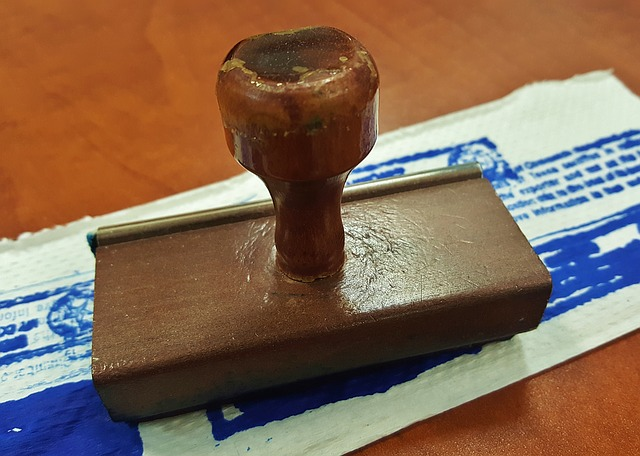
\includegraphics[width=0.5\textwidth]{../img/stamp}

\columnbreak

\pause

\begin{itemize}
\item En stämpel kan \Alert{tillverkas} -- motsvarar \Emph{deklaration} av klassen.
 \item Det händer inget förrän man \Alert{stämplar} -- motsvarar \Emph{instansiering}.
\item Då skapas \Alert{avbildningar} av stämpeln -- motsvarar \Emph{allokering av ett objekt} som är en \Emph{instans} av klassen.
\item Allokering kallas också \Emph{konstruktion} och funktionen/koden som gör själva allokeringen kallas \Emph{konstruktor}.
\end{itemize}

\end{multicols}
\end{Slide}


\begin{Slide}{Vad är en klass?}
\begin{itemize}
\item En klass är en mall \Eng{template} för att skapa objekt.
\item Objekt kan skapas med \code{new Klassnamn}, vilket kallas \Emph{instansiering}. 
\item I Scala 3 är \code{new} valfritt, det räcker med \code{Klassnamn()}. 
\item Ett objekt som skapats med en klassen \code{Klassnamn} som mall kallas för en \Emph{instans} av klassen \code{Klassnamn}.
\item En klass innehåller \Emph{medlemmar} \Eng{members}, som bl.a. kan vara:
  \begin{itemize}
  \item \Emph{attribut}, kallas även fält \Eng{field}: \code{val}, \code{lazy val}, \code{var}
  \item \Emph{metoder}, kallas även operationer: \code{def}
  \end{itemize}
\item Varje instans har sin uppsättning värden på attributen
vilka tillsammans utgör instansens \Emph{tillstånd}.
\end{itemize}

\end{Slide}
  


% \begin{Slide}[t]{Klass och instans}
% \vspace{-0.65em}
% \begin{REPLnonum}
% scala> class C { var attr = 42 }
%
% scala> val objRef1 = new C
% \end{REPLnonum}
% \vspace{3.7em}
% \begin{tikzpicture}[font=\SlideFontSmall\sffamily]
% \matrix [matrix of nodes, row sep=0, column 2/.style={nodes={rectangle,draw,minimum width=0.8cm}}] (mat)
% {
% \texttt{objRef1}   &  \makebox(10,10){ }\\
% };
%
% \node[cloud, cloud puffs=15.0, cloud ignores aspect, minimum width=2cm, minimum height=2cm,
%  align=center, draw] (instance1) at (3.8cm, 0.0cm) {
%  \begin{tabular}{r l}
%  \texttt{attr} & \fbox{42} \\
%  \end{tabular}
%  };
%
%
% \filldraw[black] ($ (mat-1-2) + (0.0cm,0.0cm) $) circle (3pt) node[] (ref1)  {};
% \draw [arrow, line width=0.7mm] (ref1) -- (instance1);
% \end{tikzpicture}
% \end{Slide}
%
%
%
% \begin{Slide}[t]{Klass och instans}
% \vspace{-0.5em}
% \begin{REPLnonum}
% scala> class C { var attr = 42 }
%
% scala> val objRef1 = new C
%
% scala> val objRef2 = new C
% \end{REPLnonum}
% \vspace{2em}
% \begin{tikzpicture}[font=\SlideFontSmall\sffamily]
% \matrix [matrix of nodes, row sep=0, column 2/.style={nodes={rectangle,draw,minimum width=0.8cm}}] (mat)
% {
% \texttt{objRef1}   &  \makebox(10,10){ }\\
% \texttt{objRef2}   &  \makebox(10,10){ }\\
% };
%
% \node[cloud, cloud puffs=15.0, cloud ignores aspect, minimum width=2cm, minimum height=2cm,
%  align=center, draw] (instance1) at (3.8cm, 0.35cm) {
%  \begin{tabular}{r l}
%  \texttt{attr} & \fbox{42} \\
%  \end{tabular}
%  };
%
% \node[cloud, cloud puffs=15.0, cloud ignores aspect, minimum width=2cm, minimum height=2cm,
%  align=center, draw] (instance2) at (5.8cm, -1.5cm) {
%  \begin{tabular}{r l}
%  \texttt{attr} & \fbox{42} \\
%  \end{tabular}
%  };
%
% \filldraw[black] ($ (mat-1-2) + (0.0cm,0.0cm) $) circle (3pt) node[] (ref1)  {};
% \draw [arrow, line width=0.7mm] (ref1) -- (instance1);
%
% \filldraw[black] ($ (mat-2-2) + (0.0cm,0.0cm) $) circle (3pt) node[] (ref2)  {};
% \draw [arrow, line width=0.7mm] (ref2) -- (instance2);
% \end{tikzpicture}
% \end{Slide}
%
%
%
% \begin{Slide}[t]{Klass och instans}
% \vspace{-0.5em}
% \begin{REPLnonum}
% scala> class C { var attr = 42 }
%
% scala> val objRef1 = new C
%
% scala> val objRef2 = new C
%
% scala> objRef2.attr = 43
% \end{REPLnonum}
% \begin{tikzpicture}[font=\SlideFontSmall\sffamily]
% \matrix [matrix of nodes, row sep=0, column 2/.style={nodes={rectangle,draw,minimum width=0.8cm}}] (mat)
% {
% \texttt{objRef1}   &  \makebox(10,10){ }\\
% \texttt{objRef2}   &  \makebox(10,10){ }\\
% };
%
% \node[cloud, cloud puffs=15.0, cloud ignores aspect, minimum width=2cm, minimum height=2cm,
%  align=center, draw] (instance1) at (3.8cm, 0.35cm) {
%  \begin{tabular}{r l}
%  \texttt{attr} & \fbox{42} \\
%  \end{tabular}
%  };
%
% \node[cloud, cloud puffs=15.0, cloud ignores aspect, minimum width=2cm, minimum height=2cm,
%  align=center, draw] (instance2) at (5.8cm, -1.5cm) {
%  \begin{tabular}{r l}
%  \texttt{attr} & \fbox{43} \\
%  \end{tabular}
%  };
%
%
% \filldraw[black] ($ (mat-1-2) + (0.0cm,0.0cm) $) circle (3pt) node[] (ref1)  {};
% \draw [arrow, line width=0.7mm] (ref1) -- (instance1);
%
% \filldraw[black] ($ (mat-2-2) + (0.0cm,0.0cm) $) circle (3pt) node[] (ref2)  {};
% \draw [arrow, line width=0.7mm] (ref2) -- (instance2);
% \end{tikzpicture}
% \end{Slide}



\begin{Slide}{Singelobjekt jämfört med klass}\SlideFontSmall
Vi har tidigare deklarerat \Emph{singelobjekt} som bara finns i \Alert{en} enda upplaga:
\begin{REPLnonum}
scala> object Björn { var ålder = 53; val längd = 178 }
\end{REPLnonum}

Med en \Emph{klass} kan man skapa \Alert{godtyckligt många} \Emph{instanser av klassen} med hjälp av nyckelordet \code{new} följt av klassens namn:

\begin{REPLnonum}
scala> class Person { var ålder = 0; var längd = 0 }

scala> val björn = new Person   // allokera plats i minnet
björn: Person = Person@7ae75ba6  // unikt id för instansen
\end{REPLnonum}
\begin{tikzpicture}[font=\small\sffamily]
\matrix [matrix of nodes, row sep=0, column 2/.style={nodes={rectangle,draw,minimum width=0.8cm}}] (mat)
{
\texttt{björn}   &  \makebox(10,10){ }\\
};
\node[cloud, cloud puffs=12.0, cloud ignores aspect, minimum width=2cm, minimum height=3.8cm,
 align=center, scale=0.8, draw] (x) at (3.8cm, -1.0cm) {
 \begin{tabular}{r l}
 \multicolumn{2}{c}{\ttfamily\itshape Person@7ae75ba6}\\ \\
 \texttt{ålder} & \fbox{~0~} \\
 \texttt{längd} & \fbox{~0~}\\
 \end{tabular}
 };
\filldraw[black] (0.6cm,0.0cm) circle (3pt) node[] (ref) {};
\draw [arrow, line width=0.7mm] (ref) -- (x);
\end{tikzpicture}
\end{Slide}


\begin{Slide}{Förändring av objektets tillstånd}
\begin{REPLnonum}
scala> björn.ålder = 53

scala> björn.längd = 178
björn: Person = Person@7ae75ba6
\end{REPLnonum}

\begin{tikzpicture}[font=\large\sffamily]
\matrix [matrix of nodes, row sep=0, column 2/.style={nodes={rectangle,draw,minimum width=0.8cm}}] (mat)
{
\texttt{björn}   &  \makebox(10,10){ }\\
};
\node[cloud, cloud puffs=13.0, cloud ignores aspect, minimum width=2cm, minimum height=3.8cm,
 align=center, draw] (x) at (5.8cm, -1.2cm) {
 \begin{tabular}{r l}
 \multicolumn{2}{c}{\ttfamily\itshape Person@7ae75ba6}\\ \\
 \texttt{ålder} & \fbox{~53~} \\
 \texttt{längd} & \fbox{~178~}\\
 \end{tabular}
 };
\filldraw[black] (0.75cm,0.0cm) circle (3pt) node[] (ref) {};
\draw [arrow, line width=0.7mm] (ref) -- (x);
\end{tikzpicture}
%{\SlideFontTiny{\ttfamily\itshape Person@7ae75ba6} är en unik idenfierare för instansen, så att JVM hittar den i heapen.}
\end{Slide}


\begin{Slide}{Bättre att initialisera med hjälp av klassparametrar}
\begin{REPLnonum}
scala> class Person(var ålder: Int, var längd: Int)

scala> val sandra = new Person(42, 166)
sandra: Person = Person@7878bbdb
\end{REPLnonum}

\begin{tikzpicture}[font=\large\sffamily]
\matrix [matrix of nodes, row sep=0, column 2/.style={nodes={rectangle,draw,minimum width=0.8cm}}] (mat)
{
\texttt{sandra}   &  \makebox(10,10){ }\\
};
\node[cloud, cloud puffs=13.0, cloud ignores aspect, minimum width=2cm, minimum height=3.8cm,
 align=center, draw] (x) at (5.8cm, -1.2cm) {
 \begin{tabular}{r l}
 \multicolumn{2}{c}{\ttfamily\itshape Person@7878bbdb}\\ \\
 \texttt{ålder} & \fbox{~42~} \\
 \texttt{längd} & \fbox{~166~}\\
 \end{tabular}
 };
\filldraw[black] (0.75cm,0.0cm) circle (3pt) node[] (ref) {};
\draw [arrow, line width=0.7mm] (ref) -- (x);
\end{tikzpicture}
%{\SlideFontTiny{\ttfamily\itshape Person@7ae75ba6} är en unik idenfierare för instansen, så att JVM hittar den i heapen.}
\end{Slide}


\begin{Slide}{Klassdeklarationer och instansiering}\SlideFontSmall
\setlength{\leftmargini}{0pt}
\begin{itemize}
\item Syntax för deklaration av klass: \\ \vspace{0.5em}{\SlideFontSize{13}{16}\code|class Klassnamn(parametrar){ medlemmar }|}\vspace{0.5em}
\item Exempel: \Emph{deklaration}
\begin{Code}
class Klassnamn(val attribut1: Int, attribut2: String){
  val attribut3: Double = 42.0              //publikt oföränderligt attribut
  private var attribut4: Boolean = false    //privat medlem syns inte utåt
  def metod(parameter: Int) = parameter + 1 //funktion i klass kallas metod
  lazy val attr5 = Vector.fill(100000)(42.0)     //fördröjd initialisering
}
\end{Code}

\item Parametrar initialiseras med de argument som ges vid \code{new}.
\item Exempel: \Emph{instansiering} med argument för initialisering av klassparametrar
\begin{Code}
val instansReferens = new Klassnamn(42, "hej")  // new är valfritt här 
\end{Code}

\item Parametrar som inte föregås av modifierare (t.ex. private val, val, var) blir \Emph{attribut} som är \code{ private[this] val } och bara är synliga i \Alert{denna} instans.
\item Attribut i klasskroppen är \Emph{publika} (alltså synliga utåt) om inte \code{private} anges.
\end{itemize}
\end{Slide}




\begin{Slide}{Övning: en klass som representerar en person}
\begin{enumerate}
  \item Deklarera en klass \code{Person} med dessa publika attribut:
  \begin{itemize}
    \item oföränderligt förnamn
    \item oföränderligt efternamn
    \item förändringsbar ålder med defaultargument \code{0}
  \end{itemize}
  \item lägg till en metod i klasskroppen med explicit returtyp som ger en 2-tupel med förnamn och efternamn
  \item skriv en deklaration som deklarerar en variabel \code{p} som initialiseras med värdet av ett uttryck som instansierar klassen \code{Person} med ditt namn och din ålder som nyfödd.
  \item skriv en sats som skriver ut ditt förnamn genom att referera attribut med punktnotation
  \item skriv en tilldelningssats som ändrar tillståndet för den instans som referensen \code{p} refererar till så att åldersattributets värde blir din nuvarande ålder
\end{enumerate}
\end{Slide}



\begin{Slide}{Lösning: klassen Person}
\begin{Code}[basicstyle=\SlideFontSize{6.9}{9}\ttfamily]
class Person(val givenName: String, val familyName: String, var age: Int = 0){
  def name: (String, String) = (givenName, familyName)
}
\end{Code}
\begin{REPLnonum}[basicstyle=\SlideFontSize{7}{9}\ttfamily\color{white}]
val p = Person("Björn", "Regnell")
println(p.name._1)
p.age = 50
\end{REPLnonum}
\end{Slide}


\begin{Slide}{Instansprivata klassparametrar}\SlideFontSmall
\setlength{\leftmargini}{0pt}

\begin{itemize}
\item Parametrar som inte föregås av modifierare (t.ex. private val, val, var) blir \Emph{attribut} som är \code{ private[this] val } och bara är synliga i \Alert{denna} instans.
\item Exempel på konsekvensen av \code{private[this]}:
\begin{REPL}[basicstyle=\SlideFontSize{6.7}{9}\ttfamily\color{white}]
scala> class C(a: Int){ def add(other: C): Int = a + other.a }
error: value a is not a member of C

// betyder samma sak som:

scala> class C(private[this] val a: Int){ def add(other: C): Int = a + other.a }
error: value a is not a member of C
\end{REPL}
\item Men detta fungerar fint:
\begin{REPL}
scala> class D(val a: Int){ def add(other: D): Int = a + other.a }

scala> D(42).add(D(43))
res0: Int = 85
\end{REPL}
...eftersom modifieraren \code{val} framför klassparameter ger publik synlighet.
\item Vad händer om du skriver \code{private val} framför klassparametern \code{a} ovan?
\end{itemize}
\end{Slide}


\begin{Slide}{\texttt{private} jämfört med \texttt{private[this]}}\SlideFontSmall
\code{private[this]} är \Alert{ännu} mer privat än \code{private}
\begin{Code}
class Hemlis(private val hemlis: Int) {
  def ärSammaSom(annan: Hemlis) = hemlis == annan.hemlis   // Funkar!
}

class Hemligare(private[this] val hemlis: Int) {
  def ärSammaSom(annan: Hemligare) = hemlis == annan.hemlis //KOMPILERINGSFEL
}
\end{Code}
\pause Vad händer om man inte skriver ens \code{val}? \pause Olika för klass och s.k. case-klass:
\begin{Code}
class Hemligare(hemlis: Int) { // motsvarar private[this] val
  def ärSammaSom(annan: Hemligare) = hemlis == annan.hemlis //KOMPILERINGSFEL
}

case class InteHemlig(seMenInteRöra: Int) { // blir automatiskt val
  def ärSammaSom(annan: InteHemlig): Boolean =
    seMenInteRöra == annan.seMenInteRöra
}

\end{Code}
{\SlideFontTiny Vi ska lära mer om det godis man får på köpet med \code{case}-klasser om ett litet tag.}
\end{Slide}



%%%%%%%%%%%% ÄR EXEMPEL KOMPLEXA TAL ÄR FÖR SVÅR MATEMATIK för lp1???? %%%%%%%%%
%% Nej komplexa tal som vektor med polära koordinater ingår i matte 4 som är krav för LTH: %%%


\begin{Slide}{Övning: Klassen Complex i Scala}\SlideFontSmall
Implementera klassen \code{Complex} nedan som representerar komplexa tal:
\begin{Code}
  class Complex(val re: Double, val im: Double):
    def r  = ???  // absolutbeloppet
    def fi = ???  // vinkeln i radianer
    def +(other: Complex): Complex = ???  // resultatet av addition
    var imSymbol = 'i'  // symbol för imaginärdel, används i toString
    override def toString = ???  // en strängrepresentation av talet
\end{Code}

\begin{minipage}{0.3\textwidth}
  Exempel: \\$z = 3 + 4i$
\end{minipage}
\begin{minipage}{0.5\textwidth}
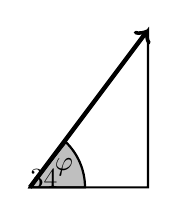
\begin{tikzpicture}[thick]
\coordinate (O) at (0,0);
\coordinate (A) at (1.5,0);
\coordinate (B) at (1.5,2.0);

%\tkzMarkAngle[fill=orange,size=0.5cm, opacity=.4](A,O,B) 
%\tkzLabelAngle[pos=0.8](A,O,B){\texttt{$\varphi$}}
 %%% AAAARGH ovan slutade funka så gjorde nedan HACK i stället
\draw[fill=lightgray, thick] (0,0) -- (0:0.7cm) arc (0:46:0.8cm) node at (30:0.5cm) {$\varphi$} -- cycle;
%\draw[fill=lightgray, thick] (0,0) -- (0:0.7cm) arc (0:45:0.8cm) node at (30:0.5cm) {$\varphi$} -- cycle;
%https://tex.stackexchange.com/questions/96459/automatically-draw-and-labels-angles-of-a-triangle-in-tikz

\draw (O)--(A)--(B)--cycle;
\draw [->, ultra thick] (O)--(B);

\tkzLabelSegment[below=5pt](O,A){\textit{real-delen} är $3$}
\tkzLabelSegment[above left=5pt](O,B){\textit{r}}
\tkzLabelSegment[right=5pt](A,B){\textit{imaginär-delen} är $4$}


\end{tikzpicture}
\end{minipage}

\end{Slide}


\begin{Slide}{Exempel: Klassen Complex i Scala}\SlideFontSmall
\scalainputlisting[basicstyle=\ttfamily\SlideFontSize{7}{9}]{../compendium/examples/complex1.scala}
%Klassparametrarna är parametrar till den s.k. \Emph{primärkonstruktorn}.
\begin{REPL}
scala> val z = new Complex(3, 4)  // konstruktion av instans av Complex
z: Complex = 3.0 + 4.0i

scala> val polärForm = (c1.r, c1.fi)
polärForm: (Double, Double) = (5.0,0.6435011087932844)

scala> val z2 = new Complex(1, 2)
z2: Complex = 1.0 + 2.0i

scala> z1 + z2
res0: Complex = 4.0 + 6.0i
\end{REPL}
\end{Slide}



\begin{Slide}{Exempel: Principen om enhetlig access}\SlideFontSmall
\scalainputlisting[basicstyle=\ttfamily\SlideFontSize{7}{9}]{../compendium/examples/complex2.scala}
\pause
\begin{itemize}
\item Efter som attributen \code{re} och \code{im} är oföränderliga, kan vi lika gärna ändra i klass-implementationen och göra om metoderna \code{r} och \code{fi} till \code{val}-variabler utan att klientkoden påverkas.

\item Då anropas \code{math.hypot} och \code{math.atan2} bara en gång vid initialisering (och inte varje gång som med \code{def}).

\item Vi skulle även kunna använda \code{lazy val} och då bara räkna ut \code{r} och \code{fi} om och när de verkligen refereras av klientkoden, annars inte.

\item Eftersom klientkoden inte ser skillnad på metoder och variabler, kallas detta \Emph{principen om enhetlig access}. (Många andra språk har \Alert{inte} denna möjlighet, tex Java där metoder \emph{måste} ha parenteser.)
\end{itemize}
\end{Slide}



\Subsection{Olika sätt att skapa instanser}

\begin{Slide}{Instansiering med direkt användning av \texttt{new}}

Instansiering genom \Emph{direkt användning} av \code{new}\\
{\SlideFontSmall (här första varianten av Complex med \code{r} och \code{fi} som metoder)}
\begin{REPLnonum}
scala> val c1 = new Complex(3, 4)
\end{REPLnonum}
\begin{tikzpicture}[font=\SlideFontSmall\sffamily]
\matrix [matrix of nodes, row sep=0, column 2/.style={nodes={rectangle,draw,minimum width=0.8cm}}] (mat)
{
\texttt{c1}   &  \makebox(10,10){ }\\
};

\node[cloud, cloud puffs=15.0, cloud ignores aspect, minimum width=2cm, minimum height=3.8cm,
 align=center, draw] (instance1) at (5.8cm, -1.5cm) {
 \begin{tabular}{r l l}
 \texttt{re:} & \texttt{Double} & \fbox{3.0} \\
 \texttt{im:} & \texttt{Double} & \fbox{4.0}\\
 \texttt{imSymbol:} & \texttt{Char} & \fbox{i}\\
 \end{tabular}
 };

\filldraw[black] ($ (mat-1-2) + (0.0cm,0.0cm) $) circle (3pt) node[] (ref1)  {};

\draw [arrow, line width=0.7mm] (ref1) -- (instance1);
\end{tikzpicture}
\pause
Ofta vill man göra \Alert{indirekt} instansiering så att vi senare har friheten att ändra hur instansiering sker.
\end{Slide}



\begin{Slide}{Indirekt instansiering med fabriksmetoder}\SlideFontSmall
En \Emph{fabriksmetod} är en metod som används för att instansiera objekt.
\begin{Code}[basicstyle=\SlideFontSize{8}{12}\ttfamily\selectfont]
object MyFactory {
  def createComplex(re: Double, im: Double) = new Complex(re, im)
  def createReal(re: Double)                = new Complex(re, 0)
  def createImaginary(im: Double)           = new Complex(0, im)
}
\end{Code}
\pause
Instansiera \Alert{inte direkt}, utan \Emph{indirekt} genom användning av \Emph{fabriksmetoder}:
\begin{REPL}
scala> import MyFactory._

scala> createComplex(3, 4)
res0: Complex = 3.0 + 4.0i

scala> createReal(42)
res1: Complex = 42.0 + 0.0i

scala> createImaginary(-1)
res2: Complex = 0.0 + -1.0i
\end{REPL}
\end{Slide}



\begin{Slide}{Hur förhindra direkt instansiering?}
Om vi vill \Emph{förhindra direkt instansiering} kan vi göra primärkonstruktorn \Alert{privat}:
\scalainputlisting[basicstyle=\ttfamily\SlideFontSize{7}{9}]{../compendium/examples/complex3.scala}
MEN... då går det ju \Alert{inte} längre att instansiera något alls!  \code{   :(}
\begin{REPLnonum}
scala> new Complex(3,4)
error:
 constructor Complex in class Complex cannot be accessed
\end{REPLnonum}
\end{Slide}



\begin{Slide}{Kompanjonsobjekt med indirekt instansiering}\SlideFontSmall
\setlength{\leftmargini}{0pt}
\begin{itemize}
\item Ett \Emph{kompanjonsobjekt} \Eng{companion object} är ett singelobjekt som ligger i \Alert{samma kodfil} som en klass, och som har \Alert{samma namn} som klassen.

\item Medlemmar i ett kompanjonsobjekt \Alert{får accessa privata} medlemmar i kompanjonsklassen (och vice versa) och kompanjonsobjektet får därför accessa privat konstruktor och kan göra \code{new}.
\scalainputlisting[basicstyle=\ttfamily\SlideFontSize{7}{9}]{../compendium/examples/complex4.scala}

\item Fabriksmetoder i kompanjonsobjektet ovan och privat konstruktor gör att vi \Alert{enbart} tillåter \Emph{indirekt instansiering}.
\end{itemize}
\end{Slide}

\begin{Slide}{Användning av kompanjonsobjekt med fabriksmetoder}
Nu kan vi \Alert{bara} instansiera \Emph{indirekt}!  \code{   :)}
\begin{REPLnonum}
scala> Complex.real(42.0)
res0: Complex = 42.0 + 0.0i

scala> Complex.imag(-1)
res1: Complex = 0.0 + -1.0i

scala> Complex.apply(3,4)
res2: Complex = 3.0 + 4.0i

scala> Complex(3,4)
res3: Complex = 3.0 + 4.0i

scala> new Complex(3, 4)
error:
     constructor Complex in class Complex cannot be accessed
\end{REPLnonum}
\end{Slide}


\begin{Slide}{Alternativa direktinstansieringar med default-argument}\SlideFontSmall
Med \Emph{default-argument} kan vi erbjuda \Emph{alternativa} sätt att direktinstansiera.
\scalainputlisting[basicstyle=\ttfamily\SlideFontSize{7}{9}]{../compendium/examples/complex5.scala}
\begin{REPL}
scala> new Complex()
res0: Complex = 0.0 + 0.0i

scala> new Complex(re = 42)  //anrop med namngivet argument
res1: Complex = 42.0 + 0.0i

scala> new Complex(im = -1)
res2: Complex = 0.0 + -1.0i

scala> new Complex(1)
res3: Complex = 1.0 + 0.0i
\end{REPL}
\end{Slide} 

\begin{Slide}{Alternativa sätt att instansiera med fabriksmetod}
Vi kan också erbjuda \Emph{alternativa} sätt att instansiera \Emph{indirekt} med fabriksmetoden \code{apply} i ett kompanjonsobjekt genom default-argument:
\scalainputlisting[basicstyle=\ttfamily\SlideFontSize{7}{9}]{../compendium/examples/complex6.scala}

\end{Slide}

\begin{Slide}{Medlemmar som bara behövs i en enda upplaga}
Attributet \code{imSymbol} passar bättre att ha i \Emph{kompanjonsobjektet}, eftersom det räcker att ha \Alert{en enda upplaga}, som kan vara gemensam för alla objekt:
\scalainputlisting[basicstyle=\ttfamily\SlideFontSize{7}{9}]{../compendium/examples/complex7.scala}

\end{Slide}



\begin{Slide}{Medlemmar i singelobjekt är statiskt allokerade}\SlideFontTiny

Minnesplatsen för \Emph{attribut i singelobjekt} allokeras automatiskt en gång för alla, och kallas därför \Emph{statiskt} allokerad. Singelobjektets namn \code{Complex} utgör en statisk referens till den enda instansen och är av typen \texttt{Complex.type}.

\begin{tikzpicture}[font=\SlideFontSmall\sffamily]
\matrix [matrix of nodes, row sep=0, column 2/.style={nodes={rectangle,draw,minimum width=0.8cm}}] (mat)
{
\texttt{Complex}   &  \makebox(10,10){ }\\
};

\node[cloud, cloud puffs=15.0, cloud ignores aspect, minimum width=1cm, minimum height=2cm,
 align=center, draw] (instance1) at (5.8cm, 0.0cm) {
 \begin{tabular}{r l l}
 \texttt{imSymbol:} & \texttt{Char} & \fbox{i}\\
 \end{tabular}
 };

\filldraw[black] ($ (mat-1-2) + (0.0cm,0.0cm) $) circle (3pt) node[] (ref1)  {};

\draw [arrow, line width=0.7mm] (ref1) -- (instance1);
\end{tikzpicture}

Nu bereder vi inte plats för \code{imSymbol} i varenda \Emph{dynamiskt} allokerade instans:
\begin{REPLnonum}
scala> val c1 = Complex(3, 4)
\end{REPLnonum}

\begin{tikzpicture}[font=\SlideFontSmall\sffamily]
\matrix [matrix of nodes, row sep=0, column 2/.style={nodes={rectangle,draw,minimum width=0.8cm}}] (mat)
{
\texttt{c1}   &  \makebox(10,10){ }\\
};

\node[cloud, cloud puffs=15.0, cloud ignores aspect, minimum width=2cm, minimum height=2cm,
 align=center, draw] (instance1) at (5.8cm, -0.0cm) {
 \begin{tabular}{r l l}
 \texttt{re:} & \texttt{Double} & \fbox{3.0} \\
 \texttt{im:} & \texttt{Double} & \fbox{4.0}\\
 \end{tabular}
 };

\filldraw[black] ($ (mat-1-2) + (0.0cm,0.0cm) $) circle (3pt) node[] (ref1)  {};

\draw [arrow, line width=0.7mm] (ref1) -- (instance1);
\end{tikzpicture}


\end{Slide}




\begin{Slide}{Attribut i kompanjonsobjekt användas för sådant som är gemensamt för alla instanser}

Om vi ändrar på statiska \code{imSymbol} så ändras \code{toString} för \Alert{alla} dynamiskt allokerade instanser.
\begin{REPLnonum}
scala> val c1 = Complex(3, 4)
c1: Complex = 3.0 + 4.0i

scala> Complex.imSymbol = 'j'
Complex.imSymbol: Char = j

scala> val c2 = Complex(5, 6)
c2: Complex = 5.0 + 6.0j

scala> c1
res0: Complex = 3.0 + 4.0j
\end{REPLnonum}
\end{Slide}


\Subsection{Case-klasser och fördelen med oföränderlighet}

\ifkompendium\else
\begin{frame}[plain]
  
\includegraphics[width=1.0\textwidth]{../img/mutant.png}
\end{frame}
\fi

\begin{Slide}{Övning: en läskig mutant}\SlideFontSmall
\begin{enumerate}
\item Skapa en klass med namnet \code{Mutant} som har ett förändringsbart attribut som klassparameter med namnet \code{i} av typen \code{Int} med default-argumentet \code{5}.
\vspace{0.5em}

\item \begin{minipage}{0.5\textwidth}
Deklarera två \code{val}-variabler som kallas \code{fem1} och \code{fem2} och som båda refererar till \Alert{samma} \code{Mutant}-instans.
\end{minipage}
\hfill\begin{minipage}{0.32\textwidth}
\hfill
\includegraphics[width=3.4cm]{../img/mutant.png}

En \code{Mutant}-instans där \code{i} kanske är fem.
\vspace{1em}
\end{minipage}

\item Skriv kod som ändrar tillstånd via den ena mutantreferensen.

\item Syns ändringen via den andra mutantreferensen?
\end{enumerate}
\end{Slide}




\begin{Slide}{Case-klasser}
Case-klasser är ett smidigt sätt att skapa \Emph{oföränderliga} datastrukturer. Med nyckelordet \code{case} framför \code{class} får du mycket ''godis på köpet'':

\begin{itemize}
\item Klassparametrar blir automatiskt publika oföränderliga attribut\footnote{alltså \Alert{inte} \texttt{private[this] val } som i vanliga klasser.} och du slipper alltså skriva \code{val}
\item Du får en automatisk \Emph{toString} med klassens namn och värdet av alla \code{val}-attribut som ges av klassparametrarna och du slipper alltså skriva en egen toString
\item Du får ett automatiskt kompanjonsobjekt med en fabriksmetod \code{apply} för indirekt instansiering där alla klassparametrarnas \code{val}-attribut initialiseras.
\pause
\item ... och mer därtill men mer om det senare...
\end{itemize}
\end{Slide}




\begin{Slide}{Exempel: oföränderliga case-klassen \code{Point}}

\begin{Code}[basicstyle=\SlideFontSize{10}{12}\ttfamily]
case class Point(x: Double, y: Double)
\end{Code}

\begin{REPLnonum}
scala> val p1 = Point(3, 4)
p1: Point = Point(3.0,4.0)

scala> val p2 = p1
p2: Point = Point(3.0,4.0)

scala> p1.x = 42
error: reassignment to val
\end{REPLnonum}
Vi kan utan risk dela med oss av en referens till en oföränderlig klass -- ingen kan ändra dess innehåll. (Jämför läskiga mutanten i tidigare exempel.)

\end{Slide}






\Subsection{Konstruktor}



\begin{Slide}{Vad är en konstruktor?}
\begin{itemize}
\item En \Emph{konstruktor} är den maskinkod som exekveras när klasser instansieras med \code{new}.

\item Konstruktorn skapar ett nytt objekt i minnet vid varje anrop.

\item I Scala \Alert{genererar kompilatorn} en \Emph{primärkonstruktor} åt dig med maskinkod som initialiserar alla attribut baserat på klassparametrarna som du deklarerat.

\pause

%\item I Java och många andra språk får man \Alert{explicit} skriva kod för konstruktorer med speciell syntax och göra alla initialiseringar av attribut själv, och det behövs många olika konstruktorer för att motsvara defaultargument.

\item I Scala \Emph{kan} man också skriva egna alternativa s.k. \Emph{hjälpkonstruktorer}, men det är \Alert{ovanligt}, eftersom man har möjligheten med fabriksmetoder i kompanjonsobjekt och default-argument.
\end{itemize}
\end{Slide}


\begin{Slide}{Hjälpkonstruktorer i Scala (ovanliga)}%\SlideFontSmall
Fördjupning för kännedom:
\begin{itemize}
\item I Scala kan man skapa ett alternativ till primärkonstruktorn, en så kallad \Emph{hjälpkonstruktor} \Eng{auxilliary constructor} genom att deklarera en metod med det speciella namnet \code{this}.


\item Hjälpkonstruktorer \Alert{måste} börja med att anropa en \Alert{annan} konstruktor som står \Alert{före} i koden, till exempel primärkonstruktorn.
\end{itemize}

\begin{Code}
class Point(val x: Int, val y: Int, val z: Int): // primärkonstruktor
  def this(x: Int, y: Int) = this(x, y, 0) // anropa primärkonstruktorn
  def this(x: Int) = this(x, 0) // anropa hjälpkonstruktor
\end{Code}

%{\SlideFontSmall Överlagrade hjälpkonstruktorer i Scala liknar användning av konstruktorer i Java, där man inte har default-argument och apply i kompanjonsobj. etc.}

\end{Slide}

\begin{Slide}{Användning av hjälpkonstruktor}
\begin{REPL}
scala> val p1 = Point(1)
p1: Point = Point@21312342

scala> val p2 = Point(1, 2)
p2: Point = Point@43254325

scala> val p3 = Point(1, 2, 3)
p3: Point = Point@346654
\end{REPL}
\pause
Men man gör \Alert{mycket oftare} så här i Scala:
\begin{Code}[basicstyle=\ttfamily\SlideFontSize{8.5}{12}]
case class Point(x: Int, y: Int = 0, z: Int = 0)
\end{Code}
Använd alltså defaultargument hellre än hjälpkonstruktor.\\
(Eller överlagrad fabriksmetod i kompanjonsobjekt.)
\end{Slide}



% \begin{Slide}{Vad gör skräpsamlaren?}\SlideFontSmall
% \begin{itemize}
% \item Scala och Java är båda programmeringsspråk som förutsätter en körmiljö med \Alert{automatisk}  \Emph{skräpsamling} \Eng{garbage collection}.
%
% \item \Emph{Skräpsamlaren} \Eng{the garbage collector} är ett program som automatiskt körs i bakgrunden då och då och \Emph{städar minnet} genom att frigöra den plats som upptas av \Alert{objekt som inte längre används}.
%
% \item JVM:en bestämmer själv när skräpsamlaren ska jobba och programmeraren har ingen kontroll över detta.
%
% \item Den stora \Emph{fördelen} med automatisk skärpsamling är att man slipper bry sig om det svåra och felbenägna arbetet att \Alert{avallokera} minne.
%
% \item \Alert{Nackdelen} är att man inte kan styra exakt hur och när skräpsamlingen ska ske och man kan därmed inte bestämma när processorn ska belastas med minneshanteringen. Detta är normalt inget problem, utom i vissa tidskritiska realtidssystem med hårda minnesbegränsningar och svarstidskrav.
%
% \item I språk utan automatisk skräpsamling, t.ex. C++, måste man ta hand om destruktion av objekt och skriva egna s.k. \Emph{destruktorer}.
% \end{itemize}
% \end{Slide}


\Subsection{Referens saknas: \texttt{null}}

\begin{Slide}{Referens saknas: \texttt{null}}
\begin{itemize}
\item I Java och många andra språk använder man ofta literalen \code{null} för att representera att ett \Alert{värde saknas}.

\item En referens som är \code{null} refererar inte till någon instans.

\item Om du försöker referera till instansmedlemmar med punktnotation genom en referens som är \code{null} kastas ett \Alert{undantag} \code{NullPointerException}.

\item Oförsiktig användning av \code{null} är en vanlig källa till \Alert{buggar}, som kan vara svåra att hitta och fixa.

\end{itemize}
\end{Slide}


\begin{Slide}{Exempel: \texttt{null}}
\begin{REPL}
scala> class Gurka(val vikt: Int)

scala> var g: Gurka = null        // ingen instans allokerad än
val g: Gurka = null

scala> g.vikt
java.lang.NullPointerException

scala> g = Gurka(42)          // instansen allokeras
val g: Gurka = Gurka@1ec7d8b3

scala> g.vikt
val res0: Int = 42

scala> g = null         // instansen kommer att destrueras av skräpsamlaren
\end{REPL}

\begin{itemize} \SlideFontSmall
\item Scala har \code{null} av kompabilitetsskäl, men det är brukligt att \Alert{endast} använda \code{null} om man anropar Java-kod.

\item Scala erbjuder smidiga \code{Option}, \code{Some} och \code{None} för säker hantering av saknade värden; mer om detta kommande vecka.



\end{itemize}
\end{Slide}


\Subsection{Referensen \texttt{this}}
\begin{Slide}{Referensen \texttt{this}}\SlideFontSmall
\begin{itemize}
\item Nyckelordet \code{this} ger en referens till den aktuella instansen.
\begin{REPLnonum}
scala> class Gurka(var vikt: Int){def jagSjälv = this}

scala> val g = Gurka(42)
val g: Gurka = Gurka@5ae9a829

scala> g.jagSjälv
val res0: Gurka = Gurka@5ae9a829

scala> g.jagSjälv.vikt
val res1: Int = 42

scala> g.jagSjälv.jagSjälv.vikt
val res2: Int = 42
\end{REPLnonum}
\item Referensen \code{this} används ofta för att komma runt ''namnkrockar'' där variabler med samma namn gör så att den ena variabeln inte syns.
\end{itemize}
\end{Slide}



\Subsection{Getters och setters}

\begin{Slide}{Getters och setters}\SlideFontSmall
\begin{itemize}
\item I många språk (t.ex. Java, Python) finns inget motsvarande nyckelord \code{val} som garanterar oföränderliga attributreferenser.
\footnote{Java har visserligen \jcode{final} men det är annorlunda som vi ska se senare.}

\item Därför gör man i dessa språk nästan alltid alla attribut \Alert{privata} för att förhindra att de ändras på ett okontrollerat sätt.

% \item Många språk följer \Alert{inte} principen om enhetlig access: åtkomst av metoder och variabler sker med olika syntax.

\item Därför är det normalt att införa metoder som kallas \Emph{getters} och \Emph{setters}, som används för att \Alert{indirekt} läsa och uppdatera \Emph{attribut}.

\item Dessa metoder känns i många språk igen genom konventionen att de heter något som börjar med \Emph{get} respektive \Emph{set}. (Men \Alert{ej} vanligt i Scala.)

\item Med \Emph{indirekt access} av attribut kan man åstadkomma \Emph{flexibilitet}, så att implementationen kan ändras utan att ändra i klientkoden:
\begin{itemize}\SlideFontSmall
\item[--] man kan t.ex. i efterhand ändra representation av de privata attributen eftersom all access sker genom getters och setters.
\end{itemize}

\item Man kan åstadkomma \Emph{oföränderliga} datastrukturer där attributreferenserna inte förändras efter allokering om klassen \Alert{inte} erbjuder en \Alert{setter} för privata attribut.
\end{itemize}
\end{Slide}



\begin{Slide}{Java-exempel: Klassen JPerson}\SlideFontSmall
\Emph{Indirekt} access av \Alert{privata} attribut:
\vspace{-1em}\begin{multicols}{2}
\javainputlisting[basicstyle=\SlideFontSize{7}{8}\ttfamily\selectfont]{../compendium/examples/JPerson.java}

\columnbreak

\begin{REPLnonum}[basicstyle=\SlideFontSize{7}{9}\ttfamily\color{white}]
$ javac JPerson.java
$ scala
Welcome to Scala 2.11.8 (Java HotSpot(TM) 64-Bit Server VM, Java 1.8.0_66).
Type in expressions for evaluation. Or try :help.

scala> val p = new JPerson("Björn")
p: JPerson = JPerson@7e774085

scala> p.getAge
res0: Int = 0

scala> p.setAge(42)

scala> p.getAge
res1: Int = 42

scala> p.age
error:
value age is not a member of JPerson
\end{REPLnonum}
\end{multicols}
\end{Slide}


\begin{Slide}{Motsvarande JPerson men i Scala}
Så här brukar man åstadkomma ungefär motsvarande i Scala: \\~
\begin{Code}[basicstyle=\SlideFontSize{12}{15}\ttfamily\selectfont]
class Person(val name: String):
  var age = 0
\end{Code}
~\\
Notera att alla attribut här är \Emph{publika}.
\end{Slide}


\begin{Slide}{Förhindra felaktiga attributvärden med setters}\SlideFontSmall
Med hjälp av \Emph{setters} kan vi förhindra \Alert{felaktig} uppdatering av attributvärden, till exempel \Alert{negativ ålder} i klassen \code{JPerson} i Java:
\begin{Code}[language=Java]
    public void setAge(int age){
        if (age >= 0) {
            this.age = age;
        } else {
            this.age = 0;
        }
    }
\end{Code}
Hur kan vi åstadkomma \Emph{motsvarande i Scala}? \\
\pause
Antag att vi började med nedan variant, men \Alert{ångrar} oss och sedan vill införa funktionalitet som förhindrat negativ ålder \Emph{utan att ändra i klientkod}:
\begin{Code}
class Person(val name: String):
  var age = 0
\end{Code}
Om vi inför en ny metod \code{setAge} och gör attributet \code{age} privat så funkar det \Alert{inte} längre att skriva  \code{ p.age = 42 } och vi ''kvaddar'' klientkoden! \code{  :(}
\end{Slide}



\begin{Slide}{Getters och setters i Scala}\SlideFontSmall
\setlength{\leftmargini}{0pt}
\begin{itemize}
\item Principen om \Emph{enhetlig access} tillsammans med \Alert{specialsyntax} för \Emph{setters} kommer till vår räddning!

\item
En \Emph{setter} kan i Scala skapas med \textbf{procedur vars namn slutar med} \texttt{\_=}
\pause
\item I Scala kan man utan att kvadda klientkod införa getter+setter så här:
\end{itemize}
\begin{Code}
class Person(val name: String): // ändrad implementation men samma access
  private var myPrivateAge = 0
  def age = myPrivateAge         // getter
  def age_=(a: Int): Unit =      // setter
    if (a >= 0) myPrivateAge = a else myPrivateAge = 0
\end{Code}
\pause\vspace{-0.5em}
\begin{REPL}
scala> val p = Person("Björn")
val p: Person = Person@28ac3dc3

scala> p.age = 42      // najs syntax om getter parad med setter enl ovan
val p.age: Int = 42

scala> p.age = -1      // nu förhindras negativ ålder
val p.age: Int = 0
\end{REPL}
\end{Slide}

%%%%%%%%%%%%%% TODO BORTPRIORITERADE SLIDES NEDAN MEN KANSKE BRA EXEMPEL SOM SKA IN IGEN??? %%%%%%%%%%%%%%%%%%%%

% \begin{Slide}{Med punktnotation kan förändringsbara variabler tilldelas nya värden och objektets tillstånd uppdateras.}
% \begin{REPLnonum}
% scala> björn.ålder = 49
% scala> björn.längd = 178
% \end{REPLnonum}
%
% \begin{tikzpicture}[font=\large\sffamily]
% \matrix [matrix of nodes, row sep=0, column 2/.style={nodes={rectangle,draw,minimum width=0.8cm}}] (mat)
% {
% \texttt{björn}   &  \makebox(10,10){ }\\
% };
% \node[cloud, cloud puffs=13.0, cloud ignores aspect, minimum width=2cm, minimum height=3.8cm,
%  align=center, draw] (x) at (5.8cm, -1.5cm) {
%  \begin{tabular}{r l}
%  \multicolumn{2}{c}{\ttfamily\itshape Person@7ae75ba6}\\ \\
%  \texttt{ålder} & \fbox{~49~~} \\
%  \texttt{längd} & \fbox{~178}\\
%  \end{tabular}
%  };
% \filldraw[black] (0.75cm,0.0cm) circle (3pt) node[] (ref) {};
% \draw [arrow, line width=0.7mm] (ref) -- (x);
% % \node[cloud, cloud puffs=15.7, cloud ignores aspect, %minimum width=5cm, minimum height=2cm,
% % align=center, draw] (g2) at (5cm, -2cm) {Gurka-\\objekt};
% % \filldraw[black] (0.4cm,-0.4cm) circle (3pt) node[] (g2ref) {};
% % \draw [arrow] (g2ref) -- (g2);
% \end{tikzpicture}
% \end{Slide}
%
%
%
%
%
% \begin{Slide}{En klass kan ha parametrar som initialiserar attribut}
% \begin{itemize}
% \item Med en parameterlista efter klassnamnet får man en så kallad \Emph{primärkonstruktor} för initialisering av attribut.
% \item Argumenten för initialiseringen ges vid \code{new}.
% \begin{REPLnonum}
% scala> class Person(var ålder: Int, var längd: Int)
%
% scala> val björn = new Person(49, 178)
% björn: Person = Person@354baab2
%
% scala> println(s"Björn är ${björn.ålder} år gammal.")
% Björn är 49 år gammal.
%
% scala> björn.ålder = 18
%
% scala> println(s"Björn är ${björn.ålder} år gammal.")
% Björn är 18 år gammal.
% \end{REPLnonum}
% \end{itemize}
% \end{Slide}
%
%
%
%
% \begin{Slide}{En klass kan ha privata medlemmar}
% Med \code{private} blir en medlem \Emph{privat}: access utifrån \Alert{medges ej}.
%
% \vspace{0.1em}
% \begin{REPL}
% scala> class Person(private var minÅlder: Int, private var minLängd: Int){
%          def ålder = minÅlder
%        }
%
% scala> val björn = new Person(42, 178)
% björn: Person = Person@4b682e71
%
% scala> println(s"Björn är ${björn.ålder} år gammal.")
% Björn är 42 år gammal.
%
% scala> björn.minÅlder = 18
% error: variable minÅlder in class Person cannot be accessed in Person
%
% scala> björn.längd
% error: value längd is not a member of Person
% \end{REPL}
% Med \code{private} kan man förhindra tokiga förändringar.
% \end{Slide}
%
%
% \begin{Slide}{Privata förändringsbara attribut och publika metoder}
% \begin{Code}
% class Människa(val födelseLängd: Double, val födelseVikt: Double){
%   private var minLängd = födelseLängd
%   private var minVikt  = födelseVikt
%   private var ålder    = 0
%
%   def längd = minLängd  // en sådan här metod kallas "getter"
%   def vikt  = minVikt   // vi förhindrar attributändring "utanför" klassen
%
%   val slutaVäxaÅlder      = 18
%   val tillväxtfaktorLängd = 0.00001
%   val tillväxtfaktorVikt  = 0.0002
%
%   def ät(mat: Double): Unit = {
%     if (ålder < slutaVäxaÅlder) minLängd += tillväxtfaktorLängd * mat
%     minVikt += tillväxtfaktorVikt * mat
%   }
%
%   def fyllÅr: Unit = ålder += 1
%
%   def tillstånd: String = s"Tillstånd: $minVikt kg, $minLängd cm, $ålder år"
% }
% \end{Code}
% \end{Slide}
%
% \begin{Slide}{Tillstånd kan förändras indirekt genom metodanrop}
% \begin{REPL}
% scala> val björn = new Människa(födelseVikt=3.5, födelseLängd=52.1)
% björn: Människa = Människa3e52
%
% scala> björn.tillstånd
% res0: String = Tillstånd: 3.5 kg, 52.1 cm, 0 år
%
% scala> for (i <- 1 to 42) björn.fyllÅr
%
% scala> björn.tillstånd
% res2: String = Tillstånd: 3.5 kg, 52.1 cm, 42 år
%
% scala> björn.ät(mat=5000)
%
% scala> björn.tillstånd
% res3: String = Tillstånd: 4.5 kg, 52.1 cm, 42 år
% \end{REPL}
% \end{Slide}
%
%
%
% \begin{Slide}{Metoden \texttt{isInstanceOf} och rot-typen \texttt{Any}}
% \SlideFontSmall\vspace{-0.5em}
% \begin{multicols}{2}
%
% \begin{REPL}
% scala> class X(val i: Int)
%
% scala> val a = new X(42)
% a: X = X@117b2cc6
%
% scala> a.isInstanceOf[X]
% res0: Boolean = true
%
% scala> val b = new X(42)
% b: X = X@61ab6521
%
% scala> b.isInstanceOf[X]
% res1: Boolean = true
%
% scala> a == b
% res2: Boolean = false
%
% scala> a.i == b.i
% res3: Boolean = true
%
% \end{REPL}
%
% \columnbreak
%
%
% \begin{itemize}\SlideFontTiny
%
% \item Ett objekt skapat med \code{new X} är en instans av \Emph{typen} \code{X}.
%
% \item Detta kan testas med metoden \code{isInstanceOf[X]: Boolean}
%
% \pause
%
% \item Typen \Emph{\texttt{Any}} är sypertyp till \Alert{alla} typer och kallas för \Emph{rot-typ} i Scalas  typhierarki.
%
% \begin{REPL}
% scala> a.isInstanceOf[Any]
% res4: Boolean = true
%
% scala> b.isInstanceOf[Any]
% res5: Boolean = true
%
% scala> 42.isInstanceOf[Any]
% res6: Boolean = true
%
% \end{REPL}
% \item Se quickref sid 4. (Mer i w10.)
% \item I klassen \href{http://www.scala-lang.org/api/current/scala/Any.html}{\code{Any}} finns bl.a. \code{toString}
% \end{itemize}
% \end{multicols}
% \end{Slide}
%
%
%
% \begin{Slide}{Överskugga \texttt{toString}}
% Alla objekt får automatiskt en metod \code{toString} som ger en sträng med objektets unika identifierare, här \texttt{Gurka@3830f1c0}:
% \begin{REPL}
% scala> class Gurka(val vikt: Int)
%
% scala> val g = new Gurka(42)
% g: Gurka = Gurka@3830f1c0
%
% scala> g.toString
% res0: String = Gurka@3830f1c0
% \end{REPL}
% Man kan \Emph{överskugga} den automatiska \code{toString}  med en \Alert{egen implementation}. Observera nyckerordet \code{override}.
% \begin{REPL}
% scala> class Tomat(val vikt: Int){override def toString = s"Tomat($vikt g)"}
%
% scala> val t = new Tomat(142)
% t: Tomat = Tomat(142 g)
%
% scala> t.toString
% res1: String = Tomat(142 g)
%
% \end{REPL}
% \end{Slide}
%
%
%
%
%
% \begin{Slide}{Objektfabrik i kompanjonsobjekt}%\SlideFontSmall
% \begin{itemize}
% \item Om det finns ett objekt i samma kodfil med samma namn som klassen blir det objektet ett s.k.  \Emph{kompanjonsobjekt} \Eng{companion object}.
%
% \item Ett kompanjonsobjekt får \Alert{accessa privata medlemmar} i den klass till vilken objektet är kompanjon.
%
% \item Kompanjonsobjekt är en bra plats för s.k. \Emph{fabriksmetoder} som skapar instanser. Då slipper vi skriva \code{new}.
% \begin{REPL}
% scala> :paste   // måste skrivas tillsammans annars ingen kompanjon
%
% class Broccoli(var vikt: Int)
%
% object Broccoli {
%   def apply(vikt: Int) = new Broccoli(vikt)
% }
%
% scala> val b = Broccoli(420)
% b: Broccoli = Broccoli@32e8d5a4
% \end{REPL}
%
% \end{itemize}
% \end{Slide}
%
%
% \begin{Slide}{Kompanjonsobjekt kan accessa privata medlemmar}%\SlideFontSmall
% \begin{Code}
% class Gurka(startVikt: Double) {
%   private var vikt = startVikt
%   def ät(tugga: Int): Unit = if (vikt > tugga) vikt -= tugga else vikt = 0
%   override def toString = s"Gurka($vikt)"
% }
% object Gurka {
%   private var totalVikt = 0.0
%   def apply(): Gurka = {
%     val g = new Gurka(math.random() * 0.42 + 0.1)
%     totalVikt += g.vikt  // hade blivit kompileringsfel om ej vore kompanjon
%     g
%   }
%   def rapport: String = s"Du har skapat ${totalVikt.toInt} kg gurka."
% }
% \end{Code}
% \pause
% \begin{REPL}
% scala> val gs = Vector.fill(1000)(Gurka())
% gs: scala.collection.immutable.Vector[Gurka] =
%   Vector(Gurka(0.49018400799506734), Gurka(0.2462822679714138), Gurka(0.17391397513818804), Gurka(0.5146514905924656), Gurka(0.47077333689159606)
%
% scala> println(Gurka.rapport)
% Du har skapat 305 kg gurka.
%
% \end{REPL}
%
% \end{Slide}
%
%
%
% \begin{Slide}{Förändringsbara och oföränderliga objekt}
% Ett \Emph{oföränderligt objekt} där nya instanser skapas i stället för tillståndsändring ''på plats''.
% \begin{Code}
% class Point(val x: Int, val y: Int) {
%   def moved(dx: Int, dy: Int): Point = new Point(x + dx, y + dy)
%
%   override def toString: String = s"Point($x, $y)"
% }
% \end{Code}
%
% Ett \Alert{förändringsbart} objekt där \Alert{tillståndet uppdateras}.
% \begin{Code}
% class MutablePoint(private var x: Int, private var y: Int) {
%   def move(dx: Int, dy: Int): Unit = {x += dx; y += dy}  // Mutation!!!
%
%   override def toString: String = s"MutablePoint($x, $y)"
% }
% \end{Code}
% \end{Slide}
%
%
% \begin{Slide}{Oföränderliga objekt}
%
% \begin{minipage}{0.5\textwidth}
% \begin{REPL}
% scala> var p1 = new Point(3, 4)
% p1: Point = Point(3, 4)
%
% scala> val p2 = p1.moved(2, 3)
% p2: Point = Point(5, 7)
%
% scala> println(p1)
% Point(3, 4)
%
% scala> p1 = new Point(0, 0)
% p1: Point = Point(0, 0)
% \end{REPL}
% \end{minipage}
% \pause\begin{minipage}{0.49\textwidth}
% {\SlideFontSmall \hfill Minnessituationen efter rad 7:}
%
% \vspace{1em}
% \begin{tikzpicture}[font=\SlideFontSmall\sffamily,scale=0.75, every node/.style={scale=0.75}]
% \matrix [matrix of nodes, row sep=0, column 2/.style={nodes={rectangle,draw,minimum width=0.6cm}}] (mat)
% {
% \texttt{p1}   &  \makebox(7,7){ }\\
% };
% \node[cloud, cloud puffs=13.0, cloud ignores aspect, minimum width=2cm, minimum height=1cm,
%  align=center, draw] (x) at (3cm, -0.0cm) {
%  \begin{tabular}{r l}
%  \texttt{x} & \fbox{~3~} \\
%  \texttt{y} & \fbox{~4~}\\
%  \end{tabular}
%  };
% \filldraw[black] (0.25cm,0.0cm) circle (3pt) node[] (ref) {};
% \draw [arrow, line width=0.5mm] (ref) -- (x);
% \end{tikzpicture}
%
% \begin{tikzpicture}[font=\SlideFontSmall\sffamily,scale=0.75, every node/.style={scale=0.75}]
% \matrix [matrix of nodes, row sep=0, column 2/.style={nodes={rectangle,draw,minimum width=0.6cm}}] (mat)
% {
% \texttt{p2}   &  \makebox(7,7){ }\\
% };
% \node[cloud, cloud puffs=13.0, cloud ignores aspect, minimum width=2cm, minimum height=1cm,
%  align=center, draw] (x) at (3cm, -0.0cm) {
%  \begin{tabular}{r l}
%  \texttt{x} & \fbox{~5~} \\
%  \texttt{y} & \fbox{~7~}\\
%  \end{tabular}
%  };
% \filldraw[black] (0.25cm,0.0cm) circle (3pt) node[] (ref) {};
% \draw [arrow, line width=0.5mm] (ref) -- (x);
% \end{tikzpicture}
%
% \end{minipage}
%
% \end{Slide}
%
%
%
% \begin{Slide}{Oföränderliga objekt}
%
% \begin{minipage}{0.5\textwidth}
% \begin{REPL}
% scala> var p1 = new Point(3, 4)
% p1: Point = Point(3, 4)
%
% scala> val p2 = p1.moved(2, 3)
% p2: Point = Point(5, 7)
%
% scala> println(p1)
% Point(3, 4)
%
% scala> p1 = new Point(0, 0)
% p1: Point = Point(0, 0)
% \end{REPL}
% \end{minipage}
% \begin{minipage}{0.49\textwidth}
% {\SlideFontSmall \hfill Minnessituationen efter rad 10:}
%
% \vspace{1em}
% \begin{tikzpicture}[font=\SlideFontSmall\sffamily,scale=0.75, every node/.style={scale=0.75}]
% \node[cloud, cloud puffs=13.0, cloud ignores aspect, minimum width=2cm, minimum height=1cm,
%  align=center, draw] (x) at (3cm, 2.0cm) {
%  \begin{tabular}{r l}
%  \texttt{x} & \fbox{~3~} \\
%  \texttt{y} & \fbox{~4~}\\
%  \end{tabular}
%  };
%
%  \node[left of=x, text width=2.5cm,align=right] (text) at (1,2) {kommer att raderas av skräpsamlaren:};
% \end{tikzpicture}
%
% \begin{tikzpicture}[font=\SlideFontSmall\sffamily,scale=0.75, every node/.style={scale=0.75}]
% \matrix [matrix of nodes, row sep=0, column 2/.style={nodes={rectangle,draw,minimum width=0.6cm}}] (mat)
% {
% \texttt{p2}   &  \makebox(7,7){ }\\
% };
% \node[cloud, cloud puffs=13.0, cloud ignores aspect, minimum width=2cm, minimum height=1cm,
%  align=center, draw] (x) at (3cm, -0.0cm) {
%  \begin{tabular}{r l}
%  \texttt{x} & \fbox{~5~} \\
%  \texttt{y} & \fbox{~7~}\\
%  \end{tabular}
%  };
% \filldraw[black] (0.25cm,0.0cm) circle (3pt) node[] (ref) {};
% \draw [arrow, line width=0.5mm] (ref) -- (x);
% \end{tikzpicture}
%
% \begin{tikzpicture}[font=\SlideFontSmall\sffamily,scale=0.75, every node/.style={scale=0.75}]
% \matrix [matrix of nodes, row sep=0, column 2/.style={nodes={rectangle,draw,minimum width=0.6cm}}] (mat)
% {
% \texttt{p1}   &  \makebox(7,7){ }\\
% };
% \node[cloud, cloud puffs=13.0, cloud ignores aspect, minimum width=2cm, minimum height=1cm,
%  align=center, draw] (x) at (3cm, -0.0cm) {
%  \begin{tabular}{r l}
%  \texttt{x} & \fbox{~0~} \\
%  \texttt{y} & \fbox{~0~}\\
%  \end{tabular}
%  };
% \filldraw[black] (0.25cm,0.0cm) circle (3pt) node[] (ref) {};
% \draw [arrow, line width=0.5mm] (ref) -- (x);
% \end{tikzpicture}
%
% \end{minipage}
%
% \pause\vspace{1em}Vi kan \Emph{lugnt dela referenser} till vårt oföränderliga objekt eftersom det \Emph{aldrig} kommer att ändras.
%
% \end{Slide}
%
%
% \newcommand{\MutaVarning}{\vspace{2em}\Alert{Varning!} Vem som helst som har tillgång till en referens till ditt förändringsbara objekt kan \Alert{manipulera} det, vilket ibland ger överaskande och \Alert{problematiska} konsekvenser!}
%
%
%
% \begin{Slide}{Förändringsbara objekt}
%
% \begin{minipage}{0.5\textwidth}
% \begin{REPL}
% scala> val mp1 = new MutablePoint(3, 4)
% mp1: MutablePoint = MutablePoint(3, 4)
%
% scala> val mp2 = mp1
% mp2: MutablePoint = MutablePoint(3, 4)
%
% scala> mp1.move(2,3)
%
% scala> println(mp2)
% MutablePoint(5, 7)
% \end{REPL}
% \end{minipage}
% \begin{minipage}{0.49\textwidth}
% {\SlideFontSmall \hfill Minnessituationen efter rad 4:}
%
% \vspace{1em}
% \begin{tikzpicture}[font=\SlideFontSmall\sffamily,scale=0.75, every node/.style={scale=0.75}]
% \matrix [matrix of nodes, row sep=0.5cm, column 2/.style={nodes={rectangle,draw,minimum width=0.6cm}}] (mat)
% {
% \texttt{mp1}   &  \makebox(7,7){ }\\
% \texttt{mp2}   &  \makebox(7,7){ }\\
% };
% \node[cloud, cloud puffs=13.0, cloud ignores aspect, minimum width=2cm, minimum height=1cm,
%  align=center, draw] (x) at (3cm, -0.0cm) {
%  \begin{tabular}{r l}
%  \texttt{x} & \fbox{~3~} \\
%  \texttt{y} & \fbox{~4~}\\
%  \end{tabular}
%  };
% \filldraw[black] (0.35cm,0.65cm) circle (3pt) node[] (ref1) {};
% \draw [arrow, line width=0.5mm] (ref1) -- (x);
%
% \filldraw[black] (0.35cm,-0.65cm) circle (3pt) node[] (ref2) {};
% \draw [arrow, line width=0.5mm] (ref2) -- (x);
%
%
% \end{tikzpicture}
%
% \end{minipage}
%
% \pause\MutaVarning
% \end{Slide}
%
%
%
%
% \begin{Slide}{Förändringsbara objekt}
%
% \begin{minipage}{0.5\textwidth}
% \begin{REPL}
% scala> val mp1 = new MutablePoint(3, 4)
% mp1: MutablePoint = MutablePoint(3, 4)
%
% scala> val mp2 = mp1
% mp2: MutablePoint = MutablePoint(3, 4)
%
% scala> mp1.move(2,3)
%
% scala> println(mp2)
% MutablePoint(5, 7)
% \end{REPL}
% \end{minipage}
% \begin{minipage}{0.49\textwidth}
% {\SlideFontSmall \hfill Minnessituationen efter \Alert{rad 7}:}
%
% \vspace{1em}
% \begin{tikzpicture}[font=\SlideFontSmall\sffamily,scale=0.75, every node/.style={scale=0.75}]
% \matrix [matrix of nodes, row sep=0.5cm, column 2/.style={nodes={rectangle,draw,minimum width=0.6cm}}] (mat)
% {
% \texttt{mp1}   &  \makebox(7,7){ }\\
% \texttt{mp2}   &  \makebox(7,7){ }\\
% };
% \node[cloud, cloud puffs=13.0, cloud ignores aspect, minimum width=2cm, minimum height=1cm,
%  align=center, draw] (x) at (3cm, -0.0cm) {
%  \begin{tabular}{r l}
%  \texttt{x} & \fbox{~5~} \\
%  \texttt{y} & \fbox{~7~}\\
%  \end{tabular}
%  };
% \filldraw[black] (0.35cm,0.65cm) circle (3pt) node[] (ref1) {};
% \draw [arrow, line width=0.5mm] (ref1) -- (x);
%
% \filldraw[black] (0.35cm,-0.65cm) circle (3pt) node[] (ref2) {};
% \draw [arrow, line width=0.5mm] (ref2) -- (x);
%
%
% \end{tikzpicture}
%
% \end{minipage}
%
% \MutaVarning
% \end{Slide}
%
%
%
% \Subsection{Case-klasser}
%
% \begin{Slide}{Vad är en case-klass?}\SlideFontSmall
% \setlength{\leftmargini}{0pt}
% \begin{itemize}
% \item En \code{case}-klass är ett smidigt sätt att skapa \Emph{oföränderliga objekt}.
% \item Kompilatorn ger dig \Alert{en massa ''godis''} på köpet (ca 50-100 rader kod), inkl.:
% \begin{itemize}\SlideFontTiny
% \item klassparametrar blir automatiskt \code{val}-attribut, alltså \Emph{publika} och \Emph{oföränderliga},
% \item en automatisk \Emph{\texttt{toString}} som visar klassparametrarnas värde,
% \item ett automatiskt \Emph{kompanjonsobjekt} med \Emph{fabriksmetod} så du slipper skriva \code{new},
% \item automatiska metoden \Emph{\texttt{copy}} för att skapa kopior med andra attributvärden, m.m...
% \end{itemize}
%
% \pause
% \item Det \Alert{enda} du behöver göra är att lägga till nyckelordet \code{case} före \code{class}...
% \end{itemize}
%
% \vspace{-0.5em}\begin{REPLnonum}
% scala> case class Point(x: Int, y: Int)
%
% scala> val p = Point(3, 5)
% p: Point = Point(3,5)
%
% scala> p.  // tryck TAB och se lite av allt case-klass-godis
% scala> Point.  // tryck TAB och se ännu mer godis
%
% scala> val p2 = p.copy(y= 30)
% p2: Point = Point(3,30)
% \end{REPLnonum}
%
%
% \end{Slide}
%
%
% \begin{Slide}{Exempel på case-klasser}
% \begin{Code}
% case class Person(namn: String, ålder: Int) {
%   def fyllerJämt: Boolean = ålder % 10 == 0
%   def hyllning = if (fyllerJämt) "Extra grattis!" else "Vi gratulerar!"
%   def ärLikaGammalSom(annan: Person) = ålder == annan.ålder
% }
%
% case class Point(x: Int = 0, y: Int = 0) {
%   def distanceTo(other: Point) = math.hypot(x - other.x, y - other.y)
%   def dx(d: Int): Point = copy(x + d, y)
%   def dy(d: Int): Point = copy(y= y + d)  //namngivet arg. och defaultarg.
% }
% object Point {
%   def origin = new Point()
% }
% \end{Code}
%
% \begin{REPL}
% scala> Point().dx(10).dy(10).dx(32)
% res0: Point = Point(42,10)
%
% scala> Point(3,4) distanceTo Point.origin
% res1: Double = 5.0
%
% \end{REPL}
% \end{Slide}

%!TEX encoding = UTF-8 Unicode
%!TEX root = ../lect-w05.tex

%%%


\Subsection{Likhet}
\begin{Slide}{Referenslikhet eller strukturlikhet?}\SlideFontSmall
Det finns två \Alert{principiellt olika} sorters \Emph{likhet}:
\begin{itemize}
\item \Emph{Referenslikhet} \Eng{reference equality} där två referenser anses lika om de refererar till \Emph{samma instans} i minnet.
\item \Emph{Strukturlikhet} \Eng{structural equality} där två referenser anses lika om de refererar till instanser med \Emph{samma innehåll}.

\pause

\item I Scala finns flera metoder som testar likhet:
\begin{itemize}\SlideFontSmall
\item metoden \code{eq} testar referenslikhet och \code{r1.eq(r2)} ger \code{true} om \code{r1} och \code{r2} refererar till \Emph{samma} instans.

\item metoden \code{ne} testar referens\textbf{o}likhet och \code{r1.ne(r2)} ger \code{true} om \code{r1} och \code{r2} refererar till \Alert{olika} instanser.

\item metoden \code{==} som anropar metoden \code{equals} som default testar referenslikhet men som \Alert{kan överskuggas} om man \Emph{själv vill bestämma} om det ska vara referenslikhet eller strukturlikhet.
\end{itemize}

\pause

\item Scalas \Emph{standardbibliotek} och \Emph{grundtyperna} \code{Int}, \code{String} etc. testar \Emph{strukturlikhet} genom metoden \code{==}
\pause
\item I Java är det annorlunda: symbolen \code{==} är ingen metod i Java utan specialsyntax som  testar referenslikhet mellan instanser, medan metoden \code{equals} kan överskuggas med valfri likhetstest.
\end{itemize}
\end{Slide}


\begin{Slide}{Exempel: referenslikhet och strukturlikhet}
I Scalas standardbibliotek har man överskuggat \code{equals} så att metoden \code{==} ger test av \Emph{strukturlikhet} mellan instanser:
\begin{REPL}
scala> val v1 = Vector(1,2,3)
v1: scala.collection.immutable.Vector[Int] = Vector(1, 2, 3)

scala> val v2 = Vector(1,2,3)
v2: scala.collection.immutable.Vector[Int] = Vector(1, 2, 3)

scala> v1 eq v2                //referenslikhetstest: olika instanser
res0: Boolean = false

scala> v1 ne v2
res1: Boolean = true

scala> v1 == v2                //strukturlikhetstest: samma innehåll
res2: Boolean = true

scala> v1 != v2
res3: Boolean = false
\end{REPL}
\end{Slide}


\begin{Slide}{Referenslikhet och egna klasser}
Om du inte gör något speciellt med dina egna klasser så ger metoden \code{==} test av \Emph{referenslikhet} mellan instanser:
\begin{REPLnonum}
scala> class Gurka(val vikt: Int)

scala> val g1 = new Gurka(42)
g1: Gurka = Gurka@2cc61b3b

scala> val g2 = new Gurka(42)
g2: Gurka = Gurka@163df259

scala> g1 == g2       // samma innehåll men olika instanser
res0: Boolean = false

scala> g1.vikt == g2.vikt
res1: Boolean = true
\end{REPLnonum}
\end{Slide}

\ifkompendium\else
\fi

%!TEX encoding = UTF-8 Unicode
%!TEX root = ../lect-w05.tex

%%%

\begin{Slide}{Case-klasser ger innehållslikhet}
Förutom annat ''godis på köpet'' får du med \code{case class} även detta:
\begin{itemize}
\item Metoden \code{==} ger \Emph{innehållslikhet} (och inte referenslikhet).
\end{itemize}
\end{Slide}



\begin{Slide}{Likhet och case-klasser}
Metoden \code{equals} är i case-klasser automatiskt överskuggad så att metoden \code{==} ger test av strukturlikhet.
\begin{REPL}
scala> case class Gurka(vikt: Int)

scala> val g1 = Gurka(42)
g1: Gurka = Gurka(42)

scala> val g2 = Gurka(42)
g2: Gurka = Gurka(42)

scala> g1 eq g2          // olika instanser
res0: Boolean = false

scala> g1 == g2          // samma innehåll!
res1: Boolean = true
\end{REPL}
\end{Slide}



\begin{Slide}{Sammanfattning case-klass-godis}
Kom-ihåg-lista med ''godis'' i \code{case}-klasser så här långt:
\begin{enumerate}
\item klassparametrar blir \code{val}-attribut
\item najs toString
\item automatisk fabriksmetod \code{apply} i kompanjonsobjekt
\item == ger innehållslikhet \Eng{structural equality}
\pause~\\...
\end{enumerate}

\vspace{1em}Men vi har inte sett allt godis än: \\Mönstermatchning (mer om det senare).
\end{Slide}

%!TEX encoding = UTF-8 Unicode
%!TEX root = ../lect-w05.tex

%%%


\Subsection{Implementation saknas: ???}

\begin{Slide}{Implementation saknas: ???}
\begin{itemize}
\item Ofta vill man bygga kod iterativt och steg för steg lägga till olika funktionalitet.

\item Standardfunktionen \code{???} ger vid anrop undantaget \Alert{\texttt{NotImplementedError}} och kan användas på platser i koden där man ännu inte är färdig.

\item \code{???} tillåter \Emph{kompilering av ofärdig kod}.

\pause

\item Undantag har bottentypen \code{Nothing} som är subtyp till \emph{alla} typer och kan därmed tilldelas referenser av godtycklig typ.

\begin{REPLnonum}
scala> lazy val sprängsSnart: Int = ???

scala> sprängsSnart + 42
scala.NotImplementedError: an implementation is missing
\end{REPLnonum}

\end{itemize}
\end{Slide}

\begin{Slide}{Exempel: ofärdig kod}
\begin{Code}[basicstyle=\SlideFontSize{9}{11}\ttfamily\selectfont]
case class Person(name: String, age: Int):
  def ärTonåring = age >= 13 && age <= 19
  def ärUng = !ärGammal
  def ärGammal: Boolean = ???   //def ännu ej bestämd
\end{Code}
\begin{REPLnonum}
scala> Person("Björn", 51).ärTonåring
res23: Boolean = false

scala> Person("Sandra", 39).ärUng
scala.NotImplementedError: an implementation is missing
\end{REPLnonum}
\end{Slide}


% \Subsection{Klass-specifikationer}
%
%
%
%
% \begin{Slide}{Specifikationer av klasser i Scala}\footnotesize
% \begin{itemize}
% \item Specifikationer av klasser innehåller information som \emph{den som ska implementera} klassen behöver veta.
% \item Specifikationer innehåller liknande information som dokumentationen av klassen (scaladoc), som beskriver vad \emph{användaren} av klassen behöver veta.
% \end{itemize}
% \begin{ScalaSpec}{Person}
% /** Encapsulate immutable data about a Person: name and age. */
% case class Person(name: String, age: Int = 0){
%   /** Tests whether this Person is more than 17 years old. */
%   def isAdult: Boolean = ???
% }
% \end{ScalaSpec}
% \begin{itemize}
% \item Specifikationer av Scala-klasser utgör i denna kurs ofullständig kod som kan kompileras utan fel.
% \item Saknade implementationer markeras med \code{???}
% \item \Emph{Dokumentationskommentarer} utgör \Alert{krav} på implementationen.
% \end{itemize}
%
% \end{Slide}
%
%
% \begin{Slide}{Specifikationer av klasser och objekt}
% \begin{ScalaSpec}{MutablePerson}
% /** Encapsulates mutable data about a person. */
% class MutablePerson(initName: String, initAge: Int){
%   /** The name of the person. */
%   def getName: String = ???
%
%   /** Update the name of the Person */
%   def setName(name: String): Unit = ???
%
%   /** The age of this person. */
%   def getAge: Int = ???
%
%   /** Update the age of this Person */
%   def setAge(age: Int): Unit = ???
%
%   /** Tests whether this Person is more than 17 years old. */
%   def isAdult: Boolean = ???
%
%   /** A string representation of this Person, e.g.: Person(Robin, 25) */
%   override def toString: String = ???
% }
% object MutablePerson {
%   /** Creates a new MutablePerson with default age. */
%   def apply(name: String): MutablePerson = ???
% }
% \end{ScalaSpec}
%
% \end{Slide}
%
% \ifkompendium
% Man brukar inte använda \code{get} och \code{set} i metodnamn i Scala. Mer senare om principen om enhetlig access \Eng{uniform access principle} och hur man gör ''setters'' som möjliggör tilldelningssyntax.
% \fi

% \ifkompendium
% \begin{Slide}{Specifikationer av Java-klasser på extentor}
% \begin{itemize}\small
% \item Specificerar signaturer för konstruktorer och metoder.
% \item Kommentarerna utgör krav på implementationen.
% \item Används flitigt på extentor i EDA016, EDA011, EDA017...
% \item Javaklass-specifikationerna \Alert{saknar} \Emph{implementationer} och behöver kompletteras med metodkroppar och klassrubriker innan de kan kompileras.
% \end{itemize}
% \begin{JavaSpec}{class Person}
% /** Skapar en person med namnet name och åldern age. */
% Person(String name, int age);

% /** Ger en sträng med denna persons namn. */
% String getName();

% /** Ändrar denna persons ålder. */
% void setAge(int age);

% /** Anger åldersgränsen för när man blir myndig. */
% static int adultLimit = 18;
% \end{JavaSpec}
% \end{Slide}
% \fi


%%!TEX encoding = UTF-8 Unicode
\chapter{Klasser}\label{chapter:W05}
Begrepp som ingår i denna veckas studier:
\begin{itemize}[noitemsep,label={$\square$},leftmargin=*]
\item objektorientering
\item klass
\item instans
\item Point
\item Square
\item Complex
\item Any
\item isInstanceOf
\item toString
\item new
\item null
\item this
\item accessregler
\item private
\item private[this]
\item klassparameter
\item primär konstruktor
\item fabriksmetod
\item alternativ konstruktor
\item förändringsbar
\item oföränderlig
\item case-klass
\item kompanjonsobjekt
\item referenslikhet
\item innehållslikhet
\item eq
\item ==\end{itemize}


%!TEX encoding = UTF-8 Unicode
%!TEX root = ../exercises.tex

\ifPreSolution

\Exercise{\ExeWeekFIVE}\label{exe:W05}

\begin{Goals}
%!TEX encoding = UTF-8 Unicode

%!TEX root = ../compendium1.tex

\item Kunna deklarera klasser med klassparametrar.
\item Kunna skapa instanser med \code{new}.
\item Kunna ge argument vid instansiering.
\item Förstå innebörden av referensvariabler och värdet \code{null}.

\item Kunna använda nyckelordet \code{private} för att styra synlighet av attribut och konstruktorparametrar.

\item Förstå syftet med getters och setters.
\item Kunna förklara accessregler för kompanjonsobjekt.
\item Kunna skapa fabriksmetod i kompanjonsobjekt.
\item Känna till nyttan med en privat konstruktor.

%\item Kunna implementera en klass utifrån en specifikation.
\item Förstå skillnaden mellan referenslikhet och strukturlikhet.
\item Känna till skillnaden mellan \code{==} och \code{eq}, samt \code{!=} och \code{ne}.

\item Kunna förklara hur case-klasser hanterar instansiering.
\item Känna till hur case-klasser hanterar likhet.

\end{Goals}

\begin{Preparations}
\item \StudyTheory{05}
\end{Preparations}

\else


\ExerciseSolution{\ExeWeekFIVE}


\fi


\BasicTasks %%%%%%%%%%%


\WHAT{Para ihop begrepp med beskrivning.}

\QUESTBEGIN

\Task \what

\vspace{1em}\noindent Koppla varje begrepp med den (förenklade) beskrivning som passar bäst:

\begin{ConceptConnections}
  klass & 1 & & A & hjälpfunktion för att anropa konstruktor \\ 
  instans & 2 & & B & upplaga av ett objekt med eget tillståndsminne \\ 
  konstruktor & 3 & & C & skapar instans, allokerar plats för tillståndsminne \\ 
  klassparameter & 4 & & D & olika instanser anses lika om de har samma tillstånd \\ 
  fabriksmetod & 5 & & E & en mall för att skapa flera instanser av samma typ \\ 
  referenslikhet & 6 & & F & ge argument vid konstruktion, initialisera tillstånd \\ 
  innehållslikhet & 7 & & G & ser privata medlemmar i klassen med samma namn \\ 
  case-klass & 8 & & H & slipper skriva new; automatisk innehållslikhet \\ 
  kompanjonsobjekt & 9 & & I & instanser anses olika även om de har samma tillstånd \\ 
\end{ConceptConnections}

\SOLUTION

\TaskSolved \what

\begin{ConceptConnections}
  klass & 1 & ~~\Large$\leadsto$~~ &  K & en mall för att skapa flera instanser av samma typ \\ 
  instans & 2 & ~~\Large$\leadsto$~~ &  H & upplaga av ett objekt med eget tillståndsminne \\ 
  konstruktor & 3 & ~~\Large$\leadsto$~~ &  L & skapar instans, allokerar plats för tillståndsminne \\ 
  klassparameter & 4 & ~~\Large$\leadsto$~~ &  E & binds till argument som ges vid konstruktion \\ 
  referenslikhet & 5 & ~~\Large$\leadsto$~~ &  J & instanser anses olika även om tillstånden är lika \\ 
  innehållslikhet & 6 & ~~\Large$\leadsto$~~ &  A & instanser anses lika om de har samma tillstånd \\ 
  case-klass & 7 & ~~\Large$\leadsto$~~ &  F & slipper skriva new; automatisk innehållslikhet \\ 
  getter & 8 & ~~\Large$\leadsto$~~ &  I & indirekt åtkomst av attributvärde \\ 
  setter & 9 & ~~\Large$\leadsto$~~ &  C & indirekt tilldelning av attributvärde \\ 
  kompanjonsobjekt & 10 & ~~\Large$\leadsto$~~ &  B & ser privata medlemmar i klass med samma namn \\ 
  fabriksmetod & 11 & ~~\Large$\leadsto$~~ &  M & hjälpfunktion för indirekt konstruktonsanrop \\ 
  \code|null| & 12 & ~~\Large$\leadsto$~~ &  G & ett värde som ej refererar till någon instans \\ 
  \code|new| & 13 & ~~\Large$\leadsto$~~ &  D & nyckelord vid direkt instansiering av klass \\ 
\end{ConceptConnections}

\QUESTEND


\WHAT{Klass och instans.}

\QUESTBEGIN

\Task \what~Du har i övning \texttt{\ExeWeekFOUR}~sett hur singelobjekt i en egen namnrymd  kan samla funktioner (metoder) och ha tillstånd (attribut). Men singelobjekt finns bara i en upplaga.

Vill du kunna skapa många objekt av samma typ behöver du en \emph{klass}. En objektupplaga som skapats ur en klass kallas en \emph{instans} av klassen. Varje instans har sitt eget tillstånd.

Deklarera singelobjektet och klassen nedan i REPL.

\begin{Code}
object Singelpunkt { var x = 1; var y = 2 }
class  Punkt       { var x = 3; var y = 2 }
\end{Code}

\Subtask  Antag att uttrycken till vänster evalueras uppifrån och ned. Vilket resultat till höger hör ihop med respektive uttryck? Prova i REPL om du är osäker.\footnote{Strängen efter \code{@}-tecknet är en hexadecimal representation av det heltal som tillordnas varje objekt för att systemet ska kunna särskilja olika instanser. \url{https://stackoverflow.com/questions/4712139}}


\begin{ConceptConnections}
  \code|Singelpunkt.x               | & 1 & & A & \code|2| \\ 
  \code|Punkt.x                     | & 2 & & B & \verb|error: not found: type| \\ 
  \code|val p  = new Singelpunkt    | & 3 & & C & \code|1| \\ 
  \code|val p1 = new Punkt          | & 4 & & D & \verb|p2: Punkt = Punkt@51ab04bd| \\ 
  \code|val p2 = new Punkt          | & 5 & & E & \code|java.lang.NullPointerException| \\ 
  \code|{ p1.x = 1; p2.x }          | & 6 & & F & \verb|p1: Punkt = Punkt@27a1a53c| \\ 
  \code|(new Punkt).y               | & 7 & & G & \code|3| \\ 
  \code|{ val p: Punkt = null; p.x }| & 8 & & H & \code|error: not found: value| \\ 
\end{ConceptConnections}

\Subtask Vid tre tillfällen blir det fel. Varför? Är det kompileringsfel eller exekveringsfel?

\SOLUTION

\TaskSolved \what

\SubtaskSolved

\begin{ConceptConnections}
  \code|Singelpunkt.x               | & 1 & ~~\Large$\leadsto$~~ &  H & \code|1| \\ 
  \code|Punkt.x                     | & 2 & ~~\Large$\leadsto$~~ &  B & \code|error: not found: value| \\ 
  \code|val p  = new Singelpunkt    | & 3 & ~~\Large$\leadsto$~~ &  A & \verb|error: not found: type| \\ 
  \code|val p1 = new Punkt          | & 4 & ~~\Large$\leadsto$~~ &  F & \verb|p1: Punkt = Punkt@27a1a53c| \\ 
  \code|val p2 = new Punkt          | & 5 & ~~\Large$\leadsto$~~ &  D & \verb|p2: Punkt = Punkt@51ab04bd| \\ 
  \code|{ p1.x = 1; p2.x }          | & 6 & ~~\Large$\leadsto$~~ &  E & \code|3| \\ 
  \code|(new Punkt).y               | & 7 & ~~\Large$\leadsto$~~ &  G & \code|2| \\ 
  \code|{ val p: Punkt = null; p.x }| & 8 & ~~\Large$\leadsto$~~ &  C & \code|java.lang.NullPointerException| \\ 
\end{ConceptConnections}

\SubtaskSolved

\noindent\begin{tabular}{l l p{5cm}}

~\\ \emph{fel} & \emph{typ} & \emph{förklaring} \\\hline

\code|error: not found: value|
& kompileringsfel & det finns ingen instans med namnet \code|Punkt|\\

\verb|error: not found: type|
& kompileringsfel & det finns ingen klass som heter \code|Singelpunkt|\\

\code|NullPointerException|
& körtidsfel & det går inte att referera attribut i en instans som inte finns\\

\end{tabular}

\QUESTEND



\WHAT{Klassparametrar.}

\QUESTBEGIN

\Task \what~Klassen punkt i föregående uppgift är inte så smidig att använda eftersom man först \emph{efter} instansiering kan ge attributen \code{x} och \code{y} de koordinatvärden man önskar och detta måste ske med explicita tilldelningssatser.

Detta problem kan du lösa med \emph{klassparametrar} som låter dig initialisera attributen med konstruktionsargument och på så sätt ange ett initialtillstånd direkt i samband med instansiering.

Deklarera klassen nedan i REPL.

\begin{Code}
class Point(var x: Int, var y: Int)
\end{Code}


\Subtask  Antag att uttrycken till vänster evalueras uppifrån och ned. Vilket resultat till höger hör ihop med respektive uttryck? Prova i REPL om du är osäker.

\begin{ConceptConnections}
  \code|val p1 = Point(1, 2)        | & 1 & & A & \verb|p2: Point = Point@218cf600| \\ 
  \code|val p2 = new Point          | & 2 & & B & \code|error: not enough arguments| \\ 
  \code|val p1 = new Point(1, 2)    | & 3 & & C & \code|2| \\ 
  \code|val p2 = new Point(3, 4)    | & 4 & & D & \code|error: not found: value| \\ 
  \code|p2.x - p1.x                 | & 5 & & E & \code|1| \\ 
  \code|(new Point(0, 1)).y         | & 6 & & F & \code|error: too many arguments| \\ 
  \code|new Point(0, 1, 2)          | & 7 & & G & \verb|p1: Point = Point@30ef773e| \\ 
\end{ConceptConnections}

\Subtask Vid tre tillfällen blir det fel. Varför? Är det kompileringsfel eller exekveringsfel?

\SOLUTION

\TaskSolved \what

\SubtaskSolved

\begin{ConceptConnections}
  \code|val p1 = Point(1, 2)        | & 1 & ~~\Large$\leadsto$~~ &  B & \code|error: not found: value| \\ 
  \code|val p2 = new Point          | & 2 & ~~\Large$\leadsto$~~ &  E & \code|error: not enough arguments| \\ 
  \code|val p1 = new Point(1, 2)    | & 3 & ~~\Large$\leadsto$~~ &  F & \verb|p1: Point = Point@30ef773e| \\ 
  \code|val p2 = new Point(3, 4)    | & 4 & ~~\Large$\leadsto$~~ &  C & \verb|p2: Point = Point@218cf600| \\ 
  \code|p2.x - p1.x                 | & 5 & ~~\Large$\leadsto$~~ &  D & \code|2| \\ 
  \code|(new Point(0, 1)).y         | & 6 & ~~\Large$\leadsto$~~ &  G & \code|1| \\ 
  \code|new Point(0, 1, 2)          | & 7 & ~~\Large$\leadsto$~~ &  A & \code|error: too many arguments| \\ 
\end{ConceptConnections}

\SubtaskSolved

\noindent\begin{tabular}{l l p{5cm}}

  ~\\ \emph{fel} & \emph{typ} & \emph{förklaring} \\\hline

  \code|error: not found: value|
  & kompileringsfel & det finns ingen instans med namnet \code|Point|\\

  \verb|error: not enough arguments|
  & kompileringsfel  & du måste ge argument vid konstruktion av klassen \code|Point| \\

  \code|error: too many arguments|
  & kompileringsfel & antalet argument stämmer ej överens med antalet klassparametrar\\

\end{tabular}

\QUESTEND



\WHAT{Oföränderlig klass med defaultargument.}

\QUESTBEGIN

\Task \what~Det du tidigare lärt dig om parametrar och argument är tillämpligt även på klassparametrar, t.ex. defaultargument och namngivna argument. Man kan dessutom framför klassparametrar använda synlighetsmodifieraren \code{private} och nyckelorden \code{var} och \code{val}.

Om inget anges framför en klassparameter är det \code{private val} som gäller\footnote{För case-klasser, som vi ska se snart, är det i stället \code{val} som gäller (alltså inte \code{private}).}.

Deklarera nedan klass i REPL.

\begin{Code}
class Point3D(val x: Int = 0, val y: Int = 0, z: Int = 0)
\end{Code}

\Subtask Antag att uttrycken till vänster evalueras uppifrån och ned. Vilket resultat till höger hör ihop med respektive uttryck? Prova i REPL om du är osäker.

\begin{ConceptConnections}
  \code|val p1 = new Point3D        | & 1 & & A & \code|false| \\ 
  \code|val p2 = new Point3D(y = 1) | & 2 & & B & \code|Reassignment to val| \\
  \code|(new Point3D(z = 2)).z      | & 3 & & C & \verb|p1: Point3D = Point3D@2eb37eee| \\ 
  \code|p2.y = 0                    | & 4 & & D & \code|true| \\ 
  \code|p2.y == 0                   | & 5 & & E & \code|value cannot be accessed| \\
  \code|p1.x == (new Point3D).x     | & 6 & & F & \verb|p2: Point3D = Point3D@65a9e8d7|

\end{ConceptConnections}

\Subtask Vad är problemet med ovan klass om man vill använda den för att representera punkter i 3 dimensioner?

\SOLUTION

\TaskSolved \what~

\SubtaskSolved

\begin{ConceptConnections}
  \code|val p1 = new Point3D        | & 1 & ~~\Large$\leadsto$~~ &  E & \verb|p1: Point3D = Point3D@2eb37eee| \\ 
  \code|val p2 = new Point3D(y = 1) | & 2 & ~~\Large$\leadsto$~~ &  A & \verb|p2: Point3D = Point3D@65a9e8d7| \\ 
  \code|(new Point3D(z = 2)).z      | & 3 & ~~\Large$\leadsto$~~ &  B & \code|error: not found: value| \\ 
  \code|p2.y = 0                    | & 4 & ~~\Large$\leadsto$~~ &  C & \code|error: reassignment to val| \\ 
  \code|p2.y == 0                   | & 5 & ~~\Large$\leadsto$~~ &  F & \code|false| \\ 
  \code|p1.x == (new Point3D).x     | & 6 & ~~\Large$\leadsto$~~ &  D & \code|true| \\ 
\end{ConceptConnections}

\SubtaskSolved Problemet är att så som klassen \code{Point3D} är deklarerad går det inte att avläsa \code{z}-koordinaten efter att en instans konstruerats. Det vore bättre om även \code{z}-attributet är \code{val}.

\QUESTEND



\WHAT{Case-klass, \code{this}, likhet, \code{toString} och kompanjonsobjekt.}

\QUESTBEGIN

\Task \what~\\Klistra in nedan klasser i REPL.

\begin{Code}
case class Pt(x: Int = 0, y: Int = 0) {
  def moved(dx: Int = 0, dy: Int = 0): Pt = Pt(x + dx, y + dy)
}

class MutablePt(private var p: (Int, Int) = (0, 0)) {
  def x: Int = p._1
  def y: Int = p._2
  def move(dx: Int = 0, dy: Int = 0) = { p = (x + dx, y+ dy); this }
  override def toString = s"MPt($x,$y)"
}
\end{Code}

\Subtask
Antag att uttrycken till vänster evalueras uppifrån och ned. Vilket REPL-svar till höger hör ihop med respektive uttryck? Prova i REPL om du är osäker.

\begin{ConceptConnections}
  \code|val p1 = Pt(1, 2)             | & 1 & & A & \code|MPt(5,6)| \\ 
  \code|val p2 = Pt(y = 3)            | & 2 & & B & \code|false| \\ 
  \code|val p3 = MutablePt(5, 6)      | & 3 & & C & \code|Pt(0,3)| \\ 
  \code|val p4 = Mutable()            | & 4 & & D & \code|Not found| \\ 
  \code|p2.moved(dx = 1) == Pt(1, 3)  | & 5 & & E & \code|Pt(1,2)| \\ 
  \code|p3.move(dy = 1) == MutablePt(5, 7)| & 6 & & F & \code|true| \\ 
\end{ConceptConnections}

\Subtask Vilken returtyp kommer kompilatorn härleda för funktionen \code{MutablePt.move}?

\Subtask Implementera en fabriksmetod \code{apply} i ett kompanjonsobjekt till klassen \code{MutablePt} som gör att du inte behöver skriva \code{new} när du skapar instanser.

\Subtask Vad kallas sådana metoder som \code{ def x } och \code{ def y } ovan?

\SOLUTION

\TaskSolved \what~

\SubtaskSolved

\begin{ConceptConnections}
  \code|val p1 = new Pt(1,2)        | & 1 & ~~\Large$\leadsto$~~ &  A & \code|Pt(1,2)| \\ 
  \code|val p2 = Pt(y=3)            | & 2 & ~~\Large$\leadsto$~~ &  B & \code|Pt(0,3)| \\ 
  \code|val p3 = new MutablePt(5, 6)| & 3 & ~~\Large$\leadsto$~~ &  D & \code|MPt(5,6)| \\ 
  \code|val p4 = Mutable()          | & 4 & ~~\Large$\leadsto$~~ &  E & \code|error: not found: value| \\ 
  \code|p2.moved(dx=1) == Pt(1, 3)  | & 5 & ~~\Large$\leadsto$~~ &  G & \code|true| \\ 
  \code|p3.move(dy=1) == new MutablePt(5,7)| & 6 & ~~\Large$\leadsto$~~ &  F & \code|false| \\ 
  \code|p2 == p3                      | & 7 & ~~\Large$\leadsto$~~ &  C & \verb|warning: always false| \\ 
\end{ConceptConnections}


\SubtaskSolved Kompilatorn härleder \code{MutablePt} eftersom det är typen på självreferensen this.
\begin{REPL}
scala> :type new MutablePt().move()
MutablePt
\end{REPL}

\SubtaskSolved
\begin{Code}
object MutablePt {
  def apply(x: Int = 0, y: Int = 0): MutablePt = new MutablePt(x, y)
}
\end{Code}

\begin{REPL}
scala> MutablePt()
res0: MutablePt = MPt(0,0)
\end{REPL}


\SubtaskSolved En metoder som avläser (delar av) ett objekts (privata) tillstånd utan att ändra det kallas en \emph{getter}.

\QUESTEND


\WHAT{Oföränderlig Java-klass.}

\QUESTBEGIN

\Task \what~Översätt nedan Scala-klass till Java-klassen \code{JPoint3D}. Alla attribut ska vara privata (varför?). Översätt defaultargumentet till en alternativ konstruktor. Kalla getters för t.ex. \jcode{getX()}. Kör \code{javac} och testa i REPL.

\begin{Code}
class Point3D(val x: Int, val y: Int, val z: Int = 0)
\end{Code}

\SOLUTION

\TaskSolved \what~

\javainputlisting[numbers=left]{examples/JPoint3D.java}

\begin{REPL}
> atom JPoint3D.java
> javac JPoint3D.java
> ls
JPoint3D.class  JPoint3D.java
> scala
Welcome to Scala 2.12.3 (Java HotSpot(TM) 64-Bit Server VM, Java 1.8.0_121).
Type in expressions for evaluation. Or try :help.

scala> val p = new JPoint3D(1,2)
p: JPoint3D = JPoint3D@53b1a3f8

scala> p.x
<console>:13: error: value x is not a member of JPoint3D

scala> p.getX
res0: Int = 1
\end{REPL}

\QUESTEND



\WHAT{Skapa en punktklass att använda på veckans laboration.}

\QUESTBEGIN

\Task \what~
Du ska som förberedelse till laborationen skapa den oföränderliga case-klassen \code{Point} som ska beskriva en koordinat i ett kartesiskt koordinatsystem\footnote{\url{https://sv.wikipedia.org/wiki/Kartesiskt_koordinatsystem}}. Skapa kod med hjälp av en editor, t.ex. \code{atom}, i filen  \code{Point.scala} enligt följande riktlinjer:
\begin{enumerate}[noitemsep]
\item \code{Point} ska ligga i paketet \code{graphics}.

\item \code{Point} ska ha följande två publika, oföränderliga klassparametrar:
\begin{itemize}[nolistsep, noitemsep]
\item \code{x: Double} för x-koordinaten.
\item \code{y: Double} för y-koordinaten.
\end{itemize}

\item \code{Point} ska ha följande publika medlemmar (två oföränderliga attribut och två metoder):
\begin{itemize}[nolistsep, noitemsep]
\item \code{val r: Double} ska ge motsvarande polära kordinatens%
\footnote{\url{https://sv.wikipedia.org/wiki/Pol\%C3\%A4ra\_koordinater}}
 avstånd till origo.
\item \code{val theta: Double} ska ge polära kordinatens vinkel i radianer.
\item \code{def negY: Point} ska ge en ny punkt med y-koordinaten negerad.
\item \code{def +(p: Point): Point} ska ge en ny punkt vars koordinat är summan av x- respektive y-kordinaterna för denna instans och punkten \code{p}.
\end{itemize}

\item \code{Point} ska ha ett kompanjonsobjekt med en metod som konstruerar en punkt från polära koortdinater. Metoden ska ha detta huvud: \\\code{def polar(r: Double, theta: Double): Point}

\end{enumerate}

\noindent Tips vid implementation och senare användning:
\begin{itemize}
\item Du har nytta av metoderna $r = $ \code{math.hypot(x, y)} och $\theta = $ \code{math.atan2(y, x)} vid omvandling till polära koordinater:

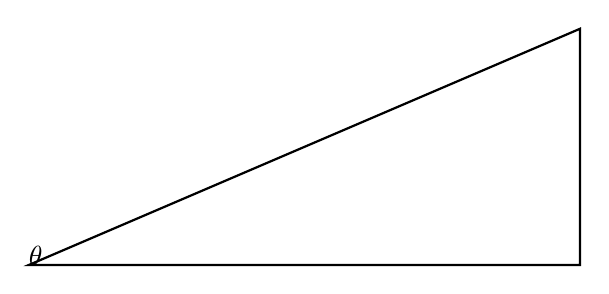
\begin{tikzpicture}[thick]
\coordinate (O) at (0,0);
\coordinate (A) at (7,0);
\coordinate (B) at (7,3);
\draw (O)--(A)--(B)--cycle;

%\tkzLabelSegment[below=2pt](O,A){\textit{adjacent leg}}
%\tkzLabelSegment[left=2pt](O,B){\textit{hypotenuse}}
%\tkzLabelSegment[above right=2pt](A,B){\textit{opposite leg}}

\tkzLabelSegment[below=5pt](O,A){\textit{x}}
\tkzLabelSegment[above left=5pt](O,B){\textit{r}}
\tkzLabelSegment[right=5pt](A,B){\textit{y}}

\tkzMarkAngle[fill= orange,size=1.5cm, opacity=.4](A,O,B)
\tkzLabelAngle[pos = 2](A,O,B){\texttt{$\theta$}}

% \tkzMarkAngle[fill= orange,size=0.65cm, opacity=.4](A,O,B)
% \tkzLabelAngle[pos = 0.35](A,O,B){$\gamma$}
%
% \tkzMarkAngle[fill= orange,size=0.8cm, opacity=.4](B,A,O)
% \tkzLabelAngle[pos = 0.6](B,A,O){$\alpha$}
%
% \tkzMarkAngle[fill= orange,size=0.7cm, opacity=.4](O,B,A)
% \tkzLabelAngle[pos = 0.5](O,B,A){$\beta$}

\end{tikzpicture}

\item Du har nytta av metoderna \code{math.cos(theta)} och \code{math.sin(theta)} vid omvandling från polära koordinater.

\item Attributet \code{negY} kommer att underlätta för dig när du på laborationen ska omvandla en punkt till fönsterkoordinater där y-axeln är omvänd jämfört med kartesiska koordinater.

\item Notera att klassens attribut är av typen \code{Double} och inte \code{Int}, trots att vi senare ska använda punkten för att beskriva en diskret pixelposition. Anledningen till detta är att det kan uppstå avrundningsfel vid numeriska beräkningar. Detta blir särskilt märkbart vid upprepad räkning med små värden, t.ex. när man ritar en approximerad cirkel med många linjesegment.
\end{itemize}

\SOLUTION

\TaskSolved \what~
\begin{Code}
package graphics

case class Point(x: Double, y: Double) {
  val r: Double          = math.hypot(x, y)
  val theta: Double      = math.atan2(y, x)
  def negY: Point        = Point(x, -y)
  def +(p: Point): Point = Point(x + p.x, y + p.y)
}
object Point {
  def polar(r: Double, theta: Double): Point =
    Point(r * math.cos(theta), r * math.sin(theta))
}
\end{Code}

\QUESTEND



\clearpage

\ExtraTasks %%%%%%%%%%%%%%%%%%%%%%%%%%%%%%%%%%%%%%%%%%%%%%%%%%%%%%%%%%%%%%%%%%%%



\WHAT{Instansiering med \code{new} och värdet \code{null}.}

\QUESTBEGIN

\Task  \what~  Man skapar instanser av klasser med \code{new}. Då anropas konstruktorn och plats reserveras i datorns minne för objektet. Variabler av referenstyp som inte refererar till något objekt har värdet \code{null}.

\Subtask Vad händer nedan? Vilka rader ger felmeddelande och i så fall hur lyder felmeddelandet?

\begin{REPL}
scala> class Gurka(val vikt: Int)
scala> var g: Gurka = null
scala> g.vikt
scala> g = new Gurka(42)
scala> g.vikt
scala> g = null
scala> g.vikt
\end{REPL}

\Subtask Rita minnessituationen efter raderna 2, 4, 6.

\SOLUTION


\TaskSolved \what


\SubtaskSolved  Rad 3 och 7 ger båda felmeddelandet \code{java.lang.NullPointerException},  på grund av försök att referera medlemmar med hjälp av en \code{null}-referens, som alltså inte pekar på något objekt.

\SubtaskSolved  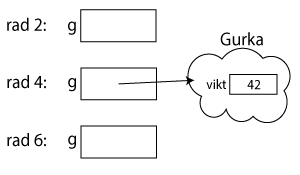
\includegraphics[scale=0.6]{../img/w06-solutions/1b}


\QUESTEND


\WHAT{Klasser,  instanser och skräp.}

\QUESTBEGIN

\Task  \what~För länge sedan i en galax långt långt borta...

\begin{Code}
case class Arm(ärTillVänster: Boolean)

case class Ben(ärTillVänster: Boolean)

case class Huvud(harHår: Boolean = true)

case class Rymdvarelse (
      arm1:   Arm   = Arm(true),
      arm2:   Arm   = Arm(false),
      ben1:   Ben   = Ben(true),
      ben2:   Ben   = Ben(false),
      huvud1: Huvud = Huvud(harHår = false),
  var huvud2: Huvud = Huvud()
) {
  def ärSkallig = !huvud1.harHår && !huvud2.harHår
}
\end{Code}

\Subtask Klistra in ovan rymdkod i REPL och evaluera nedan rader. Rita minnessituationen efter rad 5 och beskriv vad som händer.
\begin{REPL}
scala> val alien = Rymdvarelse()
scala> alien.ärSkallig
scala> val predator = Rymdvarelse()
scala> predator.ärSkallig
scala> predator.huvud2 = alien.huvud1
scala> predator.huvud2 eq alien.huvud1  // test av referenslikhet
scala> println(predator)
scala> predator.ärSkallig
\end{REPL}

\Subtask Vad händer så småningom med det ursprungliga \code{huvud2}-objektet i predator efter tilldelningen på rad 5? Går det att referera till detta objekt på något sätt?

\SOLUTION

\TaskSolved \what

\SubtaskSolved  Vi skapar två rymdvarelser, \code{alien} och \code{predator}, med vardera två ben och två armar, samt vardera två huvuden (där det ena är skalligt och det andra har hår). Efter det är varken \code{alien} eller \code{predator} skallig eftersom båda har ett huvud med hår. Sen låter man referensen till \code{predator}s huvud med hår referera till aliens huvud utan hår. Nu är predator helt skallig och delar huvud med alien.

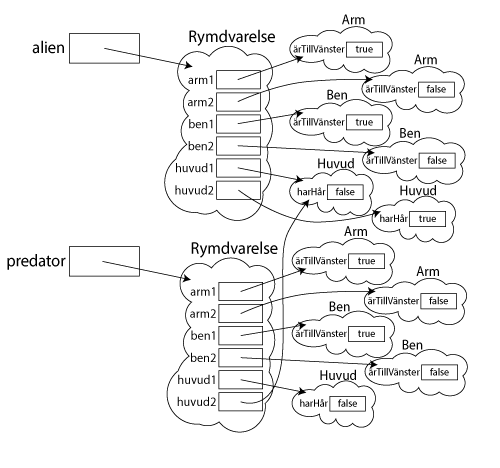
\includegraphics[scale=0.65]{../img/w06-solutions/2b}

\SubtaskSolved  Eftersom det inte längre finns någon referens som pekar på det objektet kommer skräpsamlaren att ta hand om det och det kommer förr eller senare skrivas över av något annat när platsen i minnet behövs. Objekt som inte har någon referens tills sig går inte att komma åt.

\QUESTEND




\WHAT{Case-klass. Oföränderlig kvadrat.}

\QUESTBEGIN

\Task \label{task:Square} \what~

\Subtask Implementera nedan kvadrat med en editor och klistra in den i REPL.

\begin{Code}
case class Square(val x: Int = 0, val y: Int = 0, val side: Int = 1) {
  val area: Int = ???

  /** Creates a new Square moved to position (x + dx, y + dy) */
  def moved(dx: Int, dy: Int): Square = ???

  def isEqualSizeAs(that: Square): Boolean = ???

  /** Multiplies the side with factor and rounded to nearest integer */
  def scale(factor: Double): Square = ???
}
object Square {
  /** A Square at (0, 0) with side 1 */
  val unit: Square = ???
}
\end{Code}

\Subtask Testa din kvadrat enligt nedan. Förklara vad som händer.

\begin{REPL}
scala> val (s1, s2) = (Square(), Square(1, 10, 1))
scala> val s3 = s1 moved (1,-5)
scala> s1 isEqualSizeAs s3
scala> s2 isEqualSizeAs s1
scala> s1 isEqualSizeAs Square.unit
scala> s2.scale(math.Pi) isEqualSizeAs s2
scala> s2.scale(math.Pi) isEqualSizeAs s2.scale(math.Pi)
scala> s2.scale(math.Pi) eq s2.scale(math.Pi)
scala> Square.unit eq Square.unit
\end{REPL}

\SOLUTION

\TaskSolved \what

\SubtaskSolved

\begin{Code}
case class Square(val x: Int = 0, val y: Int = 0, val side: Int = 1) {
	val area: Int = side * side

	def moved(dx: Int, dy: Int): Square = new Square(x + dx, y + dy, side)

	def isEqualSizeAs(that: Square): Boolean = this.side == that.side

	def scale(factor: Double): Square =
    Square(x, y, (side * factor).round.toInt)
}

object Square {
	val unit: Square = Square()
}
\end{Code}

\SubtaskSolved
\begin{REPL}
scala> val (s1, s2) = (Square(), Square(1, 10, 1))
s1: Square = Square(0,0,1)
s2: Square = Square(1,10,1)

scala> val s3 = s1 moved (1,-5)
s3: Square = Square(1,-5,1)

scala> s1 isEqualSizeAs s3       // lika storlek
res55: Boolean = true

scala> s2 isEqualSizeAs s1       // lika storlek
res56: Boolean = true

scala> s1 isEqualSizeAs Square.unit   // s1 har sidan 1
res57: Boolean = true

scala> s2.scale(math.Pi) isEqualSizeAs s2  // olika storlek
res58: Boolean = false

scala> s2.scale(math.Pi) == s2.scale(math.Pi) // lika innehåll
res59: Boolean = true

scala> s2.scale(math.Pi) eq s2.scale(math.Pi)  // olika objekt
res60: Boolean = false

scala> Square.unit eq Square.unit   // samma objekt
res61: Boolean = true
\end{REPL}

\QUESTEND



\WHAT{Förändrinsbar Java-klass.}

\QUESTBEGIN

\Task \what~Översätt nedan Scala-klass till Java-klassen \code{JMutablePoint3D}. Alla attribut ska vara privata (varför?). Översätt defaultargumentet till en alternativ konstruktor. Kalla setters för t.ex. \jcode{setX}. Kör \code{javac} och testa i REPL.

\begin{Code}
class MutablePoint3D(var x: Int, var y: Int, var z: Int = 0)
\end{Code}

\SOLUTION

\TaskSolved \what~

\javainputlisting[numbers=left]{examples/JMutablePoint3D.java}

\begin{REPL}
> atom JMutablePoint3D.java
> javac JMutablePoint3D.java
> ls
JMutablePoint3D.class  JMutablePoint3D.java
> scala
Welcome to Scala 2.12.3 (Java HotSpot(TM) 64-Bit Server VM, Java 1.8.0_121).
Type in expressions for evaluation. Or try :help.

scala> val p = new JMutablePoint3D(1,2)
p: JMutablePoint3D = JMutablePoint3D@2cae9b8

scala> p.x
<console>:13: error: value x is not a member of JPoint3D

scala> p.getZ
res0: Int = 0

scala> p.setZ(3)

scala> p.getZ
res1: Int = 3

\end{REPL}

\QUESTEND






\clearpage

\AdvancedTasks %%%%%%%%%%%%%%%%%%%%%%%%%%%%%%%%%%%%%%%%%%%%%%%%%%%%%%%%%%%%%%%%%


\WHAT{Attributrepresentation. Privat konstruktor. Fabriksmetod.}

\QUESTBEGIN

\Task \what~Kim Kodkunnig skapade för länge sedan denna klass som används på många ställen i befintlig kod:

\begin{Code}
class Point private (val x: Int, val y: Int)
object Point {
  def apply(x: Int = 0, y: Int = 0): Point = new Point(x, y)
  val origo = apply()
}
\end{Code}

\Subtask Vad händer om du försöker instansiera Kim Kodkunnigs klass direkt med nyckelordet \code{new}?

\Subtask Varför använder Kim Kodkunnig ett kompanjonsobjekt med en fabriksmetod? Vilka accessregler gäller mellan ett kompanjonsobjekt och klassen med samma namn?

\Subtask Hjälp Kim Kodkunnig att ändra attributrepresentationen så att det oföränderliga tillståndet utgörs av en 2-tupel \code{val p: (Int, Int)} i stället. Befintlig kod ska inte behöva ändras och klassen \code{Point} ska bete sig från ''utsidan'' precis som innan.

\SOLUTION

\TaskSolved \what~

\SubtaskSolved Det blir kompileringsfel eftersom konstruktorn är privat.
\begin{REPL}
scala> :paste

class Point private (val x: Int, val y: Int)
object Point {
  def apply(x: Int = 0, y: Int = 0): Point = new Point(x, y)
  val origo = apply()
}

scala> new Point(0,0)
<console>:14: error: constructor Point in class Point cannot be accessed
\end{REPL}

\SubtaskSolved
\begin{itemize}
  \item Genom att ha en privat konstruktor och bara göra indirekt instansiering via fabriksmetod är lätt ändra attributrepresentation i framtiden utan att befintlig kod behöver ändras.

  \item Med en \code{apply}-metod i kompansjonsobjektet kan man instansiera genom att skriva \code{Point(1, 2)} utan new.

  \item Accessreglerna för kompanjonsobjekt är sådana att kompanjoner ser varandras privata delar.
\end{itemize}

\SubtaskSolved

\begin{Code}
class Point private (private val p: (Int, Int)) {
  def x: Int = p._1
  def y: Int = p._2
}
object Point {
  def apply(x: Int = 0, y: Int = 0): Point = new Point(x, y)
  val origo = apply()
}
\end{Code}

\QUESTEND



\WHAT{Synlighet av klassparametrar och konstruktor, \code{private[this]}.}

\QUESTBEGIN

\Task  \what~

\Subtask En av gurk-klasserna nedan är trasig. Varför och vad blir det för fel?

\begin{Code}
class Gurka1(vikt: Int)

class Gurka2(val vikt: Int)

class Gurka3(private val vikt: Int)

class Gurka4(private val vikt: Int, kompis: Gurka4){
  def kompisVikt = kompis.vikt
}

class Gurka5(private[this] val vikt: Int, kompis: Gurka5){
  def kompisVikt = kompis.vikt
}

class Gurka6 private (vikt: Int)

class Gurka7 private (var vikt: Int)
object Gurka7 {
  def apply(vikt: Int) = {
    require(vikt >= 0, "negativ vikt: " + vikt)
    new Gurka7(vikt)
  }
}
\end{Code}

\Subtask Undersök nedan vad nyckelorden \code{val} och \code{private} får för konsekvenser. Förklara vad som händer. Vilka rader ger vilka felmeddelanden?

\begin{REPL}
scala> new Gurka1(42).vikt
scala> new Gurka2(42).vikt
scala> new Gurka3(42).vikt
scala> val ingenGurka: Gurka4 = null
scala> new Gurka4(42, ingenGurka).kompisVikt
scala> new Gurka4(42, new Gurka4(84, null)).kompisVikt
scala> new Gurka6(42)
scala> new Gurka7(-42)
scala> Gurka7(-42)
scala> val g = Gurka7(42)
scala> g.vikt
scala> g.vikt = -1
scala> g.vikt
\end{REPL}


\SOLUTION


\TaskSolved \what

\SubtaskSolved \code{Gurka5} är trasig. Eftersom vikten i \code{Gurka5} är privat för instansen och inte klassen kan en instans inte accessa en annan instans vikt.
\begin{REPL}
  error: value vikt is not a member of Gurka5
  def kompisVikt = kompis.vikt
\end{REPL}


\SubtaskSolved
\begin{REPL}
scala> new Gurka1(42).vikt
<console>:13: error: value vikt is not a member of Gurka1
       new Gurka1(42).vikt
                      ^

scala> new Gurka2(42).vikt
res64: Int = 42

scala> new Gurka3(42).vikt
<console>:13: error: value vikt in class Gurka3 cannot be accessed in Gurka3
       new Gurka3(42).vikt
                      ^

scala> val ingenGurka: Gurka4 = null
ingenGurka: Gurka4 = null

scala> new Gurka4(42, ingenGurka).kompisVikt
java.lang.NullPointerException
  at Gurka4.kompisVikt(<console>:13)
  ... 36 elided

scala> new Gurka4(42, new Gurka4(84, null)).kompisVikt
res67: Int = 84

scala> new Gurka6(42)
<console>:13: error: constructor Gurka6 in class Gurka6 cannot be accessed
       new Gurka6(42)
       ^

scala> new Gurka7(-42)
<console>:14: error: constructor Gurka7 in class Gurka7 cannot be accessed
       new Gurka7(-42)
       ^

scala> Gurka7(-42)
java.lang.IllegalArgumentException: requirement failed: negativ vikt: -42


scala> val g = Gurka7(42)
g: Gurka7 = Gurka7@70717ed5

scala> g.vikt
res71: Int = 42

scala> g.vikt = -1
g.vikt: Int = -1

scala> g.vikt
res72: Int = -1
\end{REPL}

\QUESTEND





\WHAT{Egendefinierad setter kombinerat med privat konstruktor.}

\QUESTBEGIN

\Task  \what~Klistra in denna kod i REPL:

\begin{Code}
class Gurka8 private (private var _vikt: Int) {
  def vikt = _vikt
  def vikt_=(v: Int): Unit = {
    require(v >= 0, "negativ vikt: " +v)
    _vikt = v
  }
}

object Gurka8 {
  def apply(vikt: Int) = {
    require(vikt >= 0, "negativ vikt: " + vikt)
    new Gurka8(vikt)
  }
}
\end{Code}


\Subtask Förklara vad som händer nedan. Vilka rader ger vilka felmeddelanden?
\begin{REPL}
scala> val g = Gurka8(-42)
scala> val g = Gurka8(42)
scala> g.vikt
scala> g.vikt = 0
scala> g.vikt = -1
scala> g.vikt += 42
scala> g.vikt -= 1000
\end{REPL}

\Subtask Vad är fördelen med möjligheten att skapa egendefinierade setters?

\SOLUTION


\TaskSolved \what


\SubtaskSolved

Rad 1:
\begin{REPL}
	java.lang.IllegalArgumentException: requirement failed: negativ vikt: -42
\end{REPL}
\code{Gurka8.apply} kräver att \code{vikt >= 0} annars kastar \code{require} ett undantag.

Rad 5:
\begin{REPL}
	java.lang.IllegalArgumentException: requirement failed: negativ vikt: -1
\end{REPL}
Settern \code{vikt_=} kräver att \code{vikt >= 0} annars kastar \code{require} ett undantag.

Rad 7:
\begin{REPL}
	java.lang.IllegalArgumentException: requirement failed: negativ vikt: -958
\end{REPL}
Eftersom \code{42 - 1000} är mindre än noll kastar \code{require} ett undantag.

\SubtaskSolved  Man kan sätta egna mer specifika krav på vad som får göras med värdena så man har större koll på att inget oväntat händer.

\QUESTEND




\WHAT{Objekt med föränderligt tillstånd \Eng{mutable state}.}

\QUESTBEGIN

\Task  \what~  Du ska implementera en modell av en hoppande groda som uppfyller följande krav:
\begin{enumerate}%[nolistsep, noitemsep]
\item Varje grodobjekt ska hålla reda på var den är.
\item Varje grodobjekt ska hålla reda på hur långt grodan hoppat totalt.
\item Varje grodobjekt ska kunna beräkna hur långt det är mellan grodans nuvarande position och utgångsläget.
\item Alla grodor börjar sitt hoppande i origo.
\item En groda kan hoppa enligt två metoder:
  \begin{itemize} [nolistsep, noitemsep]
  \item relativ förflyttning enligt parametrarna \code{dx} och \code{dy},
  \item slumpmässig relativ förflyttning $[1, 10]$ i x-ledsförändring och $[1, 10]$ i y-ledsförändring.
  \end{itemize}
\end{enumerate}

\Subtask Implementera klassen \code{Frog} enligt nedan kodskelett och ovan krav.

\begin{Code}
class Frog private (initX: Int = 0, initY: Int = 0) {
  def x: Int = ???
  def y: Int = ???

  def jump(dx: Int, dy: Int): Unit = ???
  def randomJump: Unit = ???

  def distanceToStart: Double = ???
  def distanceJumped: Double = ???
  def distanceTo(that: Frog): Double = ???
}
object Frog {
  def spawn(): Frog = ???
}
\end{Code}
\emph{Tips:}
\begin{itemize} [nolistsep, noitemsep]
\item Om namnet man vill ge ett privat föränderligt attribut ''krockar'' med ett metodnamn, är det vanligt att man börjar attributets namn med understreck, t.ex. \code{private var _x } för att på så sätt undkomma namnkonflikten.
\item Inför en metod i taget och klistra in den nya grodan i REPL efter varje utvidgning och testa.
\end{itemize}



\Subtask Skapa en metod \code{def test(): Unit} i ett singelobjekt \code{FrogTest} som innehåller kod som gör minst en kontroll av varje krav. Om ingen kontroll går fel ska \code{"Test Ok!"} skrivas ut annars ska exekveringen avbrytas. \emph{Tips:} Använd \code{assert(b, msg)} som avbryter exekveringen och skriver ut \code{msg} om \code{b} är falsk.

\Subtask Vad kallas en metod som enbart returnerar värdet av ett privat attribut?

\Subtask Inför setters för attributen som håller reda på x- och y-postitionen. Förändringar av positionen i x- eller y-led ska räknas som ett hopp och alltså registreras i det attribut som håller reda på det ackumulerade hoppavståndet.

\Subtask Simulera ett massivt grodhoppande med krockdetektering genom att skapa 100 grodor som till att börja med är placerade på x-axeln med avståndet $8$ längdenheter mellan sig. För varje runda i en \code{while}-sats, låt en slumpässigt vald groda göra ett \code{randomJump} tills någon groda befinner sig närmare än $0.5$ längdenheter, vilket är definitionen på att de har krockat. Räkna hur många looprundor som behövs innan något grodpar krockar och skriv ut antalet. Skriv även ut det totala antalet \\ \emph{Tips:} Börja med pseudokod på papper. Använd en grodvektor.


\SOLUTION


\TaskSolved \what


\SubtaskSolved
\begin{Code}
class Frog private (initX: Int = 0, initY: Int = 0) {
	private var _x: Int = initX
	private var _y: Int = initY
	private var _distanceJumped: Double = 0

  def x: Int = _x
  def y: Int = _y

	def jump(dx: Int, dy: Int): Unit = {
		_x += dx
		_y += dy
		_distanceJumped += math.hypot(dx, dy)
	}


	def randomJump: Unit = {
		def rnd = util.Random.nextInt(10) + 1
		jump(rnd, rnd)
	}

	def distanceToStart: Double = math.hypot(x,y)
	def distanceJumped: Double = _distanceJumped
	def distanceTo(f: Frog): Double = math.hypot(x - f.x, y - f.y)
}

object Frog {
	def spawn(): Frog = new Frog()
}
\end{Code}

\SubtaskSolved Exempel på testprogram:
\begin{Code}
object FrogTest {
  def test(): Unit = {
    val f1 = Frog.spawn()
    assert(f1.x == 0 && f1.y == 0, "Test of spawn, reqt 1 & 4 failed.")

    f1.jump(4,3)
    assert(f1.x == 4 && f1.y == 3, "Test of jump, reqt 1 & 4 failed.")

    f1.jump(4,3)
    assert(f1.distanceJumped == 10, "Test of jump, reqt 2 failed.")

    f1.jump(-4,-3)
    assert(f1.distanceToStart == 5, "Test of jump, reqt 3 failed.")

    for (x <- 1 to 10000) {
      val f2 = Frog.spawn()
    	f2.randomJump
    	assert(f2.x > 0 && f2.x <= 10 && f2.y > 0 && f2.y <= 10,
            "Test of randomJump, reqt 5 failed.")
    }
    println("Test Ok!")
  }
}
\end{Code}

\SubtaskSolved  En metod som är en indirekt avläsning av attrubtvärden kallas getter.

\SubtaskSolved
\begin{Code}

class Frog private (initX: Int = 0, initY: Int = 0) {
	private var _x: Int = initX
	private var _y: Int = initY
	private var _distanceJumped: Double = 0

	def jump(dx: Int, dy: Int): Unit = {
		_x += dx
		_y += dy
		_distanceJumped += math.hypot(dx, dy)
	}

	def x: Int = _x
  def x_= (newX: Int): Unit = { // Setter för x
		_distanceJumped += math.abs(x - newX)
		_x = newX
	}

  def y: Int = _y
	def y_= (newY: Int): Unit = { // Setter för y
		_distanceJumped += math.abs(y - newY)
		_y = newY
	}


	def randomJump: Unit = {
		def rnd = util.Random.nextInt(10) + 1
		jump(rnd, rnd)
	}

	def distanceToStart: Double = math.hypot(x,y)
	def distanceJumped: Double = _distanceJumped
	def distanceTo(f: Frog): Double = math.hypot(x - f.x, y - f.y)
}

object Frog {
	def spawn(): Frog = new Frog()
}

\end{Code}

\SubtaskSolved
\begin{Code}
object frogSimulation {
  def isAnyCollision(frogs: Vector[Frog]): Boolean = {
    var found = false
    frogs.indices.foreach { i =>  // generate all pairs (i,j)
      for (j <- i + 1 until frogs.size)
        if (!found) found = frogs(i).distanceTo(frogs(j)) <= 0.5
    }
    found
  }

  def jumpUntilCrash(n: Int = 100, initDist: Int = 8): (Int, Double) = {
    val frogs = Vector.fill(n)(Frog.spawn)
    (0 until n).foreach(i => frogs(i).x = i * initDistance)
    var count = 0
    while (!isAnyCollision(frogs)) {
      frogs(util.Random.nextInt(n)).randomJump
    	count += 1
    }
    (count, frogs.map(_.distanceJumped).sum)
  }

  def run(nbrOfCrashTests: Int = 10) = for (i <- 1 to nbrOfCrashTests) {
    val (n, dist) = jumpUntilCrash()
    println(s"\nAntalet looprundor innan grodkrock: $n")
    println(s"Totalt avstånd hoppat av alla grodor: $dist")
  }
}
\end{Code}

\QUESTEND




\QUESTBEGIN

\Task  \what~  Webbshoppen \textbf{UberSquare} säljer flyttbara kvadrater. I affärsmodellen ingår att ta betalt per förflyttning. Du ska hjälpa UberSquare att utveckla en enkel prototyp för att imponera på riskkapitalister.

\Subtask Implementera \code{Square} enligt dokumentationskommentarerna i efterföljande kodskiss och enligt dessa krav:

\begin{enumerate}%[nolistsep, noitemsep]
   \item Varje instans av \code{Square} ska räkna antalet förflyttningar som gjorts sedan instansen konstruerats.

   \item För att kunna övervaka sina kunder vill UberSquare även räkna det totala antalet förflyttningar som gjorts av alla kvadrater som någonsin skapats (s.k. \emph{big data}).

  \item Varje gång förflyttning sker ska ett visst belopp adderas till den ackumulerade kostnaden för respektive kvadrat, enligt kostnadsberäkningen i krav 4.

  \item UberSquare är oroliga för att kvadraterna flyttas för långt bort och bestämmer därför att för varje förflyttning ska den ackumulerade kvadratkostnaden ökas med den nya positionens avstånd till ursprungsläget vid kvadratens konstruktion multiplicerat med aktuell storlek på kvadraten.

  \item För att framstå som goda berättar UberSquare i sin marknadsföring att skala är gratis att använda. \footnote{D.v.s ett anrop av metoden \code{scale} orsakar ingen omedelbar kostnad.}
\end{enumerate}

\begin{CodeSmall}
/** A mutable and expensive Square. */
class Square private (val initX: Int, val initY: Int, val initSide: Int) {
  private var nMoves = 0;
  private var sumCost = 0.0;

  private var _x = initX;
  private var _y = initY;

  private var _side = initSide;

  private def addCost(): Unit = {
   sumCost += ???
  }

  def x: Int = ???
  def y: Int = ???

  def side = ???

  /** Scales the side of this square and rounds it to nearest integer */
  def scale(factor: Double): Unit = ???

  /** Moves this square to position (x + xd, y + dy) */
  def move(dx: Int, dy: Int): Unit = ???

  /** Moves this square to position (x, y) */
  def moveTo(x: Int, y: Int): Unit = ???

  /** The accumulated cost of this Square */
  def cost: Double = ???

  /** Returns the accumulated cost. Sets the accumulated cost to zero. */
  def pay: Double = ???

  override def toString: String =
    s"Square[($x, $y), side: $side, #moves: $nMoves times, cost: $sumCost]"
}


object Square {
  private var created = Vector[Square]()

  /** Constructs a new Square object at (x, y) with size side */
  def apply(x: Int, y: Int, side: Int): Square = {
    require(side >= 0, s"side must be positive: $side")
    ???
  }

  /** Constructs a new Square object at (0, 0) with side 1 */
  def apply(): Square = ???

  /** The total number of moves that have been made for all squares. */
  def totalNumberOfMoves: Int = ???

  /** The total cost of all squares. */
  def totalCost: Double = ???
}
\end{CodeSmall}

\Subtask Testa din kvadratprototyp i REPL. Använd t.ex. koden nedan:
\begin{REPL}
scala> val xs = Vector.fill(10)(Square())
scala> xs.foreach(_.move(2, 3))
scala> xs.foreach(_.scale(2.9))
scala> val (m, c) = (Square.totalNumberOfMoves, Square.totalCost)
m: Int = 10
c: Double = 36.055512754639885
\end{REPL}

\SOLUTION

\TaskSolved \what~

\begin{CodeSmall}
class Square private (val initX: Int, val initY: Int, val initSide: Int) {
  private var nMoves = 0;
  private var sumCost = 0.0;

  private var _x = initX;
  private var _y = initY;

  private var _side = initSide;

  private def addCost(): Unit = {
   sumCost += math.hypot(x - initX, y - initY) * side
  }

  def x: Int = _x
  def y: Int = _y

  def side = _side

  def scale(factor: Double): Unit = { _side = (_side * factor).round.toInt }

  def move(dx: Int, dy: Int): Unit = {
    _x += dx; _y += dy;
    nMoves += 1
    addCost()
  }

  def moveTo(x: Int, y: Int): Unit = {
    _x = x; _y = y;
    nMoves += 1
    addCost()
  }

  def cost: Double = sumCost

  def pay: Double = {val temp = sumCost; sumCost = 0; temp}

  override def toString: String =
    s"Square[($x, $y), side: $side, #moves: $nMoves times, cost: $sumCost]"
}
object Square {
  private var created = Vector[Square]()

  def apply(x: Int, y: Int, side: Int): Square = {
    require(side >= 0, s"side must be positive: $side")
    val sq = (new Square(x, y, side))
    created :+= sq
    sq
  }

  def apply(): Square = apply(0, 0, 1)

  def totalNumberOfMoves: Int = created.map(_.nMoves).sum

  def totalCost: Double = created.map(_.cost).sum
}
\end{CodeSmall}

\QUESTEND



\WHAT{Hjälpkonstruktor.}

\QUESTBEGIN

\Task\Uberkurs \label{task:aux-constructor} \what~I tidigare uppgifter har vi möjliggjort alternativa sätt att skapa instanser genom default-argument och fabriksmetoder i kompanjonsobjekt.

Ett annat sätt att göras detta på, som i Scala är ovanligt\footnote{Men i Java är detta mycket vanligt då defaultargument m.m. inte ingår i språket.}, är att definiera flera konstruktorer inne i klasskroppen. I Scala kallas en sådan extra konstruktor för \textbf{hjälpkonstruktor} \Eng{auxiliary constructor}.

En hjälpkonstruktor skapar man i Scala genom att definiera en metod som har det speciella namnet \code{this}, alltså en deklaration \code{def this(...) = ...} Hjälpkonstruktorer måste börja med att anropa en annan konstruktor, antingen den primära konstruktorn (d.v.s. den som klasshuvudet definierar) eller en tidigare definierad  hjälpkonstruktor.

\Subtask Läs mer om hjälpkonstruktorer här: \\ \href{http://www.artima.com/pins1ed/functional-objects.html#6.7}{www.artima.com/pins1ed/functional-objects.html\#6.7}

\Subtask Hitta på en egen uppgift med hjälpkonstruktorer, baserat på någon av klasserna i tidigare övningar.


%\Task \TODO \\ \code{class Rational private (numerator: BigInt, denominator: BigInt)} \\
%Inspirerat av Rational i pins1ed med GCD\SOLUTION

\QUESTEND

%!TEX encoding = UTF-8 Unicode

%!TEX root = ../compendium2.tex

\Lab{\LabWeekFIVE}

\begin{Goals}
%!TEX encoding = UTF-8 Unicode

%!TEX root = ../compendium2.tex

\item Kunna skapa en klass utifrån en textuell beskrivning. % av dess medlemmar.
%\item Kunna skapa en klass utifrån ofärdig kod och dokumentationskommentarer.
%\item Kunna införa privata attribut med lämpliga namn som representerar instansers förändringsbara tillstånd.
\item Kunna förklara skillnaden mellan klasser och instanser av klasser.
\item Kunna förklara skillnader och likheter mellan ett singelobjekt och objekt som är instanser av klasser.
\item Kunna förklara skillnaden mellan förändringsbara och oföränderliga objekt.
%\item Förstå innebörden av instansreferensen \code{this}.
\item Kunna skapa och använda klasser vars instanser innehåller referenser till andra instanser (aggregering).

\end{Goals}

\begin{Preparations}
\item \DoExercise{\ExeWeekFIVE}{05}

\item Läs igenom hela laborationen och studera dokumentationen för:
\begin{itemize}[nolistsep,noitemsep]
\item klassen \jcode{SimpleWindow} här: \url{http://cs.lth.se/pgk/api/}

\item \code{scala.Double} och \code{scala.math}, speciellt metoder för avrunding, trigonometri och polära koordinater, här:
\url{http://www.scala-lang.org/api/current/} 
\end{itemize}

\end{Preparations}

\subsection{Bakgrund}

Under den här laborationen ska du skapa en samling av klasser som tillsammans kan användas för att rita i ett fönster. Du ska bland annat skapa en klass \code{Turtle} som använder den färdigskrivna java-klassen \code{SimpleWindow} för att möjliggöra sköldpaddsgrafik liknande det vi gjorde i kojo-laborationen i avsnitt \ref{section:lab:kojo}. 

%SimpleWindow kan skapa ett enkelt ritfönster på skärmen, med metoder för att rita linjer, etc. SimpleWindow håller koll på en ''penna'' som representerar \textit{aktuell ritposition}. Det finns metoder för att flytta pennan och att rita en rak linje från pennans aktuella ritposition till en ny pennposition. 
%Delar av dokumentationen för SimpleWindow återspeglas i nedan specifikation. 
%Den fullständiga dokumentationen återfinns här: \url{http://cs.lth.se/pgk/api/}

%\vspace{1em}%hack to keep comment with method
%\begin{JavaSpec}{class SimpleWindow}
%  /** mouse click event type */
%	public final static int MOUSE_EVENT = 1;
%
%  /** key pressed event type */
%	public final static int KEY_EVENT = 2;
%
%  /** window closed event type */
%	public final static int CLOSE_EVENT = 3;
%
%  /** Creates a window and makes it visible. */
%	public SimpleWindow(int width, int height, String title);
%
%  /** Returns the width of the window. */
%	public int getWidth();
%
%	/** Returns the height of the window. */
%	public int getHeight();
%
%	/** Clears the window. */
%	public void clear();
%
%	/** Closes the window.*/
%	public void close();
%
%	/** Opens the window. */
%	public void open();
%
%	/** Moves the pen to a new position. */
%	public void moveTo(int x, int y) ;
%
%	/** Moves the pen to a new position while drawing a line. */
%	public void lineTo(int x, int y);
%
%	/** Writes a string at the current position.* /
%	public void writeText(String txt);
%
%	/** Draws a bitmap image at the current position.*/
%	public void drawImage(Image image);
%
%	/** Returns the pen's x coordinate. */
%	public int getX();
%
%	/** Returns the pen's y coordinate. */
%	public int getY();
%
%	/** Sets the line width.  */
%	public void setLineWidth(int width);
%
%	/** Sets the line color. */
%	public void setLineColor(Color col);
%
%	/**Returns the current line width. */
%	public int getLineWidth();
%
%	/** Returns the current line color. */
%	public Color getLineColor();
%
%	/**  Waits for a mouse click. */
%	public void waitForMouseClick();
%
%	/** Returns the mouse x coordinate at the last mouse click. */
%	public int getMouseX();
%
%	/** Returns the mouse y coordinate at the last mouse click. */
%	public int getMouseY();
%
%	/**Adds a sprite to the window. */
%	public void addSprite(Sprite sprite);
%
%	/** Wait for a specified time. */
%	public static void delay(int ms);
%\end{JavaSpec}
%
%
%\clearpage

\subsection{Obligatoriska uppgifter}


\Task Skapa dessa kataloger %(kallas även bibliotek eller mappar på svenska och \emph{''folder''} eller \emph{directory} på engelska) 
och tomma filer för din kod med hjälp av nedan linuxkommandon (eller motsvarande på annat lämpligt sätt):
\begin{REPLnonum}
mkdir turtle
cd turtle
mkdir -p src/main/scala/graphics
touch Point.scala Main.scala 
mv *.scala src/main/scala/graphics/.
ls src/main/scala/graphics/
\end{REPLnonum}
Om man skriver mycket kod blir det lättare att hitta olika delar om man har dem i olika filer med lämpliga  filnamn. Det är vanligt att man lägger kodfilerna i katalogen \code{src/main/scala} och där skapar en egen underkatalog för varje paket med samma namn som paketet.\footnote{Flera verktyg kräver exakt denna katalogstruktur för att hitta koden utan specialinställningar.} 


\Task Du ska skapa case-klassen \code{Point} som ska beskriva en koordinat i ett kartesiskt koordinatsystem\footnote{\url{https://sv.wikipedia.org/wiki/Kartesiskt_koordinatsystem}}. Skapa kod med hjälp av en editor, t.ex. \code{atom}, i filen  \code{src/main/scala/graphics/Point.scala} enligt följande riktlinjer:
\begin{enumerate}%[noitemsep]
\item Klassen \code{Point} ska vara en oföränderlig case-klass. 

\item Klassen \code{Point} ska ligga i paketet \code{graphics}.

\item Klassen \code{Point} ska ha följande två publika, oföränderliga klassparametrar:
\begin{itemize}[nolistsep, noitemsep]
\item \code{x: Double} för x-koordinaten.
\item \code{y: Double} för y-koordinaten.
\end{itemize}

\item Klassen \code{Point} ska ha följande publika medlemmar (två oföränderliga attribut och två metoder):
\begin{itemize}[nolistsep, noitemsep]
\item \code{val r: Double} ska ge motsvarande polära kordinatens%
\footnote{\url{https://sv.wikipedia.org/wiki/Pol\%C3\%A4ra\_koordinater}}
 avstånd till origo.
\item \code{val theta: Double} ska ge polära kordinatens vinkel i radianer.
\item \code{def negY: Point} ska ge en ny punkt med y-koordinaten negerad. 
\item \code{def +(p: Point): Point} ska ge en ny punkt vars koordinat är summan av x- respektive y-kordinaterna för denna instans och punkten \code{p}.
\end{itemize}

\item Klassen \code{Point} ska ha ett kompanjonsobjekt med en metod som konstruerar en punkt från polära koortdinater. Metoden ska ha detta huvud: \\\code{def polar(r: Double, theta: Double): Point}

\end{enumerate}

\noindent Tips vid implementation och senare användning:
\begin{itemize}
\item Du har nytta av metoderna \code{math.hypot(x, y)} och \code{math.atan2(y, x)} vid omvandling till polära koordinater.

\item Du har nytta av metoderna \code{math.cos(x)} och \code{math.sin(y)} vid omvandling från polära koordinater.

\item Attributet \code{negY} kommer att underlätta för dig när du i metoden \code{draw} i klassen \code{Turtle} ska omvandla en punkt till fönsterkoordinater där y-axeln är omvänd jämfört med kartesiska koordinater.

\item Notera att klassens attribut är av typen \code{Double} och inte \code{Int}, trots att vi senare ska använda punkten för att beskriva en diskret pixelposition. Anledningen till detta är att det kan uppstå avrundningsfel vid numeriska beräkningar. Detta blir särskilt märkbart vid upprepad räkning med små värden, t.ex. när man ritar en approximerad cirkel med många linjesegment.
\end{itemize}

\noindent Du ska kunna använda din punkt enligt följande exempel. Starta REPL och klistra in din case-klass med sitt kompanjonsobjekt efter kommandot \code{:paste} (eller kortare \code{:pa}). Du ska inte ta med paketdeklarationen då \code{package} inte fungerar i REPL.
\begin{REPLnonum}
scala> Point(1,1).theta.toDegrees
res0: Double = 45.0

scala> Point(3,4).r
res1: Double = 5.0

scala> Point(1,1).negY + Point(2,5)
res2: Point = Point(3.0,4.0)

scala> Point.polar(2, 60.0.toRadians).theta.toDegrees
res3: Double = 60.000001669652114
\end{REPLnonum}


\Task Lägg \code{cslib.jar} i katalogen \code{lib}, t.ex. med dessa linuxkommandon:
\begin{REPLnonum}
$ mkdir lib
$ wget -O lib/cslib.jar http://cs.lth.se/pgk/cslib
\end{REPLnonum}

\Task Skapa en \code{main}-metod i singelobjektet \code{Main} i paketet \code{graphics} i filen \code{src/main/scala/graphics/Main.scala} som gör något enkelt med både \code{Point} och \code{SimpleWindow}, t.ex. drar en linje mellan två punkter enlig nedan. 
\scalainputlisting[numbers=left,basicstyle=\ttfamily\fontsize{11}{13}\selectfont]%
{../workspace/w05_turtle/src/main/scala/graphics/Main.scala}

\noindent När många kodfiler beror av varandra behöver kompilatorn ha tillgång till alla kodfiler samtidigt.  Detta kan åstadkommas genom att ge \code{*.scala} som argument till \code{scalac} enligt nedan. Dessutom blir det en hel del \code{.class}-filer som utdata från kompilatorn, så man brukar lägga dem i en katalog med namnet \code{bin} (eller ibland \code{target}) för att separera dem från övriga filer. Använd följande linuxkommando\footnote{I Windows, byt ut kolon mot semikolon.} för att skapa \code{bin}-katalog, samkompilera alla filer och köra \code{main}-metoden:
\begin{REPLnonum}
$ mkdir bin
$ scalac -cp lib/cslib.jar -d bin src/main/scala/graphics/*.scala
$ scala -cp "lib/cslib.jar:bin" graphics.Main
\end{REPLnonum}


\Task Skapa klassen Turtle som representerar en virtuell sköldpadda med en penna under magen som kan rita i \code{SimpleWindow} enligt nedan riktlinjer:

\begin{enumerate}
\item Klassen \code{Turtle} ska vara en klass med ett förändringsbart tillstånd bestående av tre privata attribut som håller reda på detta:

\begin{itemize}
\item en position av typen \code{Point} där ett positivt y-värde räknas \emph{nedåt} i fönstret.
\item en riktning av typen \code{Double} som anges som en vinkel i grader  (och inte radianer), där ett positivt värde anger vinkeln motsols från x-axeln. 
\item ett läge på pennan av typen \code{Boolean} där \code{true} anger att pennan är nere.
\end{itemize}

\item Utgå från det ofärdiga kodskelettet nedan där dokumentationskommentarerna ger ytterligare detaljer att ta hänsyn till. Om du skriver klassen från början behöver du inte skriva av dokumentationskommentarerna. Kodskelettet finns annars i kursens \code{workspace} på GitHub%
\footnote{\url{https://github.com/lunduniversity/introprog/blob/master/workspace/}} och här: \url{http://cs.lth.se/pgk/ws}

\item Flera metoder har \code{Turtle} som returtyp. I dessa fall ska en referens till den egna instansen returneras för att möjliggöra upprepad punktnotation, t.ex.:\\
\code{t.jumpTo(Point(100, 200)).turnNorth.penDown}

\scalainputlisting[numbers=left,basicstyle=\ttfamily\fontsize{10}{12}\selectfont]%
{../workspace/w05_turtle/src/main/scala/graphics/Turtle.scala}
\end{enumerate}

\noindent Tips:

\begin{itemize}
\item Allteftersom du implementerar de saknade delarna, utöka din \code{main}-metod i \code{Main.scala} med fler tester och kolla så att dina implementationer funkar som det är tänkt. Testa på nytt efter varje litet tillägg så att du hela tiden har något som fungerar. Det är mycket lättare att felsöka efter en liten ändring än efter många och stora ändringar.

\item Du får namnge de privata variablerna som representerar det förändringsbara tillståndet så som du själv anser lämpligt. Tänk på att det i Scala kan bli namnkrock mellan metoder och privata attribut. I dessa fall brukar man namnge det privata attributet med ett understreck före för att skilja dem åt, t.ex.: \\
\code{private var _direction: Double  = ???}

\item I metoden \code{forward} har du nytta av metoden \code{Point.polar}, metoden \code{.toRadians} som kan konvertera en \code{Double} i grader till radianer, samt metoden \code{negY}. Tänk på att vinkelberäkningar på radianer förutsätter kartesiskt koordinatsystem, så negeringen av Y-axeln ska ske efter sådana beräkningar, men innan uppdatering av positionen sker. 
\end{itemize}


\Task Implementera case-klassen \code{Rect} enligt specifikationen nedan. Kodskelettet finns i workspace. Testa dina implementationer allteftersom du skriver dem, genom att stegvis utöka din \code{main}-metod.

\scalainputlisting[numbers=left,basicstyle=\ttfamily\fontsize{10.5}{12}\selectfont]%
{../workspace/w05_turtle/src/main/scala/graphics/Rect.scala}

\noindent Metoderna ovan har \code{Rect} som returtyp; en referens till den egna instansen ska returneras för att möjliggöra upprepad punktnotation, t.ex.:\\
\code{r.rotatedLeft(15).translated(0, 2).scaled(1.5)}

\clearpage

\Task\Checkpoint När \code{Turtle} och \code{Rect} är färdigimplementerade så ska du testa klasserna gemensamt genom att köra \code{main}-metoden i singelobjektet \code{Demo} nedan. Koden finns i kursens workspace. 

Den första bilden ska visa två lika stora rektanglar i samma höjd. Efter musklick kommer en animering av tre färgglada rektanglar. När det finns en handledare ledig, redovisa vad du åstadkommit. Vid väntetid, fortsätt med efterföljande uppgifter.

\scalainputlisting[numbers=left,basicstyle=\ttfamily\fontsize{11}{14}\selectfont]%
{../workspace/w05_turtle/src/main/scala/graphics/Demo.scala}


\clearpage

\subsection{Frivilliga extrauppgifter}

Nedan uppgifter kan göras i valfri ordning.

\Task Använd din Turtle för att rita en cirkel. För att göra detta kan du t.ex. låta din Turtle gå ett kort steg och svänga någon grad tills den har gjort ett fullt varv.

\Task Skapa två stycken Turtles i samma fönsterobjekt som rör sig alternerande. Fungerar allt som tänkt?


\Task Studera dokumentationen för de \code{SimpleWindow}-metoder som erbjuder hantering av händelser \Eng{event} och använd dessa för lösa deluppgifterna nedan.

\Subtask Gör så att en Turtle kan styras med hjälp av tangentbordstryckningar A--S--D--W för vänster--ner--höger--upp och att den ritar ett spår allteftersom den förflyttas.

\Subtask Gör så att en andra Turtle kan styras med hjälp av tangentbordstryckningar J--K--L--I för vänster--ner--höger--upp och att den också ritar ett spår allteftersom den förflyttas.

\Subtask Gör så att, när de två sköldpaddorna ovan befinner sig tillräckligt nära varandra, det ritas ut en rektangel med hörn där de två sköldpaddorna finns. (Denna uppgift är lite svårare och kan behöva delas upp i delar.)


\Task Studera dokumentationen för de \code{SimpleWindow}-metoder som erbjuder hantering av flyttbara bilder \Eng{sprites}. Gör så att en fin Sprite ritas vid positionen för de styrbara sköldpaddorna i föregående uppgift.


\Task Skapa en case-klass \code{RectSeq} enligt specifikation på sidan \pageref{code:classes:graphics:rectanglesequence}. I denna klass skall metoden \code{draw} rita ut ett antal rektanglar där varje rektangel har förflyttat sig, roterats och skalats jämfört med föregående rektangel i sekvensen. 

\begin{figure}[H]
\centering
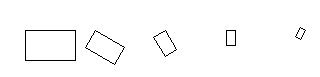
\includegraphics[width=0.75\textwidth]{../img/turtle/RectSeq.png}
%\caption Rotation av rektangel med koden nedan.
%\label{fig:classes:graphics:rollingrectangle}
\end{figure}
\noindent Bilden ovan kan skapas med hjälp av denna kod:
\begin{Code}
  def rectSeqExample(t: Turtle): Unit  = {
    val rect = Rect(pos = Point(200, 200), width = 50, height = 30)
    RectSeq(rect, n = 5, dist = 70, rot = -30, scale = 0.67).draw(t)
  }
\end{Code}

\noindent Nedan kod ritar bilden i fig. \ref{fig:classes:graphics:rectanglesequence} på sidan \pageref{fig:classes:graphics:rectanglesequence}. Använd gärna \code{setLineColor} i \code{SimpleWindow} för att göra en färggladare stjärna. Slumpvisa transformationer är också kul. 

\begin{Code}
val w = new SimpleWindow(500, 500, "Shapes")
val t = new Turtle(w, new Point(200, 200), 0, false)
val rect = Rect(pos = Point(225, 235), width = 50, height = 30)
val roll = RectSeq(rect, n = 100, dist = 2, scale = 0.98)
for (i <- 0 to 360 by 20) roll.rotatedLeft(i).draw(t)
\end{Code}


\begin{figure}
\centering
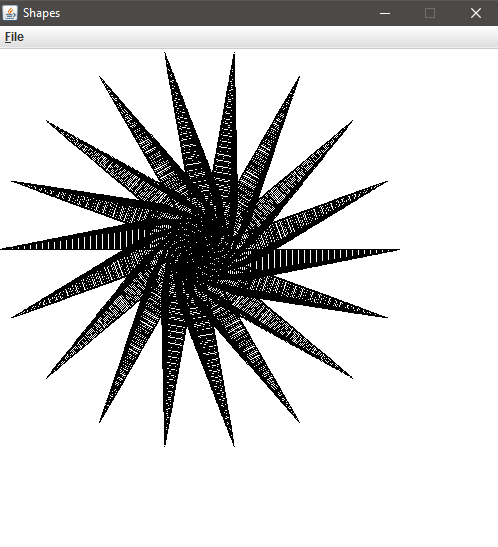
\includegraphics[width=0.5\textwidth]{../img/w06-lab/RectangleSequence.png}
\caption {En stjärna skapad med hjälp av \code{RectSeq}.}
\label{fig:classes:graphics:rectanglesequence}
\end{figure}

\noindent Nedan finns ett kodskellett som du kan utgå ifrån. Dokummentationskommentarerna innehåller fler detaljer om hur det är tänkt att klassen ska fungera. %De metoder som returnerar \code{RectSeq} ska returnera en referens till den egna instansen så att upprepad punktnotation möjliggörs.

\begin{figure}[H]
\scalainputlisting[numbers=left,basicstyle=\ttfamily\fontsize{9.9}{12}\selectfont]%
{../workspace/w05_turtle/src/main/scala/graphics/RectSeq.scala}
\label{code:classes:graphics:rectanglesequence}
\end{figure}



%\Task En riktig utmaning, för den som har lust: Implementera spelet ''Masken'' som beskrivs här: \url{https://sv.wikipedia.org/wiki/Snake}.


%!TEX encoding = UTF-8 Unicode

%!TEX root = ../compendium1.tex

%!TEX encoding = UTF-8 Unicode
\chapter{Sekvenser}\label{chapter:W06}
Begrepp som ingår i denna veckas studier:
\begin{multicols}{2}\begin{itemize}[noitemsep,label={$\square$},leftmargin=*]
\item översikt av Scalas samlingsbibliotek och samlingsmetoder
\item klasshierarkin i scala.collection
\item Traversable
\item Iterable
\item Seq
\item List
\item ListBuffer
\item ArrayBuffer
\item WrappedArray
\item sekvensalgoritm
\item algoritm: SEQ-COPY
\item in-place vs copy
\item algoritm: SEQ-REVERSE
\item registrering
\item algoritm: SEQ-REGISTER
\item linjärsökning
\item algoritm: LINEAR-SEARCH
\item tidskomplexitet
\item minneskomplexitet
\item sekvenser i Java vs Scala
\item for-sats i Java
\item java.util.Scanner
\item översikt strängmetoder
\item StringBuilder
\item ordning
\item inbyggda sökmetoder
\item find
\item indexOf
\item indexWhere
\item inbyggda sorteringsmetoder
\item sorted
\item sortWith
\item sortBy
\item variabelt argumentantal\end{itemize}\end{multicols}

\clearpage\section{Teori}
%!TEX encoding = UTF-8 Unicode
%!TEX root = ../lect-w06.tex

%%%

\ifkompendium\else
\Subsection{Veckans uppgifter}

\begin{SlideExtra}{Veckans övning: \texttt{patterns}}
  Mål: Träna på matchning och undantag
\begin{itemize}
\item Uppg. 1--8: Matchning, \code{Option}
\item Uppg. 9--11: Undantag, \code{Try}
\item Uppg. 12: Laborationsförberedelse \code{Cell} och \code{Table}
\item Uppg. 13: Matchning eller dynamisk bindning?
\item Uppg. 14: avgöra likhet med matchning, \code{equals} utan arv
\item Uppg. 15--22: diverse fördjupningsuppgifter om matchning, undantag, hash-koder, likhet vid arvshierarki
\end{itemize}
\end{SlideExtra}


\begin{SlideExtra}{Veckans labb: \texttt{tabular}}\SlideFontTiny
%  \setlength{\leftmargini}{0pt}
\hspace{-2em}\begin{minipage}{0.7\textwidth}
\vspace{0.25em}
\Emph{Förberedelse:}
\begin{itemize}
\item Gör övning \code{patterns}, speciellt uppg. 12
\item Studera givna koden: {\SlideFontTiny \href{https://github.com/lunduniversity/introprog/tree/master/workspace/w13_tabular}{workspace/w10\_tabular}}
\item Fyll i denna enkät:
\\{\SlideFontTiny \url{https://goo.gl/forms/hC6JK2UQXVpbGECc2}}
\item Se svar här (snapshot uppdateras då och då): \url{http://cs.lth.se/pgk/favorit}
\end{itemize}

\Emph{Grunduppgift:}
\begin{itemize}
\item Terminalapp för hantering av kolumndata i textfiler.
\item Matchning används vid kommandotolkning.
\item \code{Option} används för inkapsling av ev. saknade värden
\item \code{Try} används för inkapsling av ev. undantag
\end{itemize}
\Emph{Extrauppgifter:} (Minst en)
\begin{itemize}
\item dialoger: \code{load}, \code{save}, kommando: \code{pie}, \code{bar}
\end{itemize}
\end{minipage}
\hfill\begin{minipage}{0.3\textwidth}
\centering
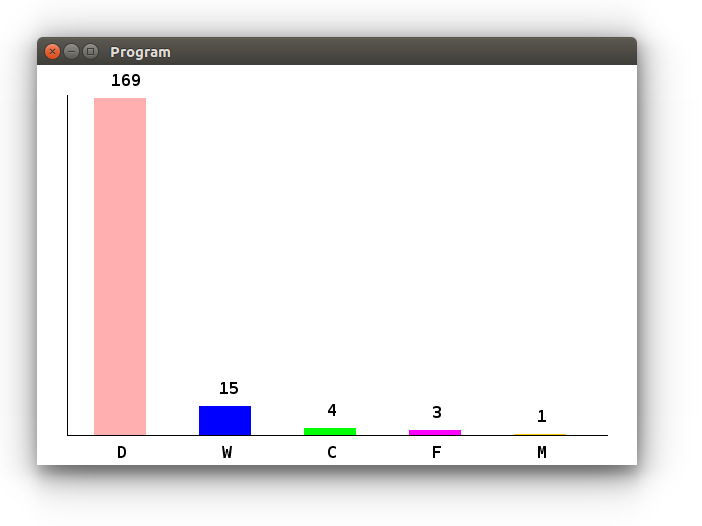
\includegraphics[width=0.95\textwidth]{../img/survey/bar}

\vspace{2em}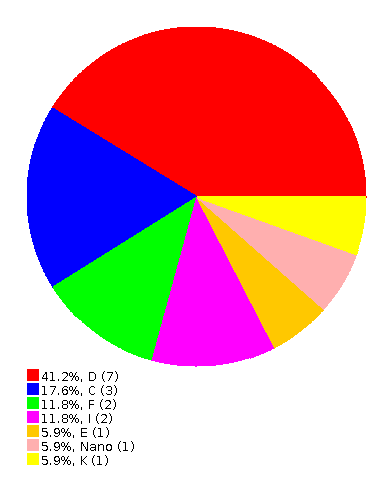
\includegraphics[width=0.7\textwidth]{../img/survey/pie}
\end{minipage}
\end{SlideExtra}

\begin{SlideExtra}{Extraundervisning del 3}
\begin{itemize}
\item  \Alert{Extraundervisning} i \Emph{E:1406} onsdag 21/11 kl 15:15-17:00
\item Hitta dit: \url{http://fileadmin.cs.lth.se/ehus/E1406.pdf}
\item Det finns gott om platser i den salen >70 platser så alla är välkomna
\item Fokus: grundläggande, långsam behandling på begäran, grumliga begrepp etc.
\end{itemize}
\end{SlideExtra}
\fi


%!TEX encoding = UTF-8 Unicode
%!TEX root = ../lect-w06.tex

%%%

\Subsection{Matchning}

\ifkompendium
\noindent  I ett match-uttryck kan man matcha på ett visst värde eller på en viss typ och match-uttryck används gärna istället för nästlade if-uttryck, då de ofta är lättare att läsa och begripa. Med match-uttryck kan man också göra \Emph{mönstermatchning} mot case-klass-instanser, t.ex. för att på ett smidigt sätt undersöka om attribut har speciella värden. Match-uttryck i Scala är en mer kraftfull variant av \code{switch}-satser som finns i många andra språk.  
\fi

\begin{Slide}{Vad är matchning?}

  \begin{itemize}
    \item Matchning gör man då man vill jämföra ett värde mot andra värden och hitta överensstämmelse \Eng{match} enligt olika \Emph{mönster}.
    \item Med mönster kan man även \Alert{plocka isär} objekt i sina beståndsdelar.
  \end{itemize}
\end{Slide}

\begin{Slide}{Plocka isär ett objekt i sina beståndsdelar med mönster}

\begin{REPLnonum}
scala> case class Point(x: Int, y: Int)

scala> val p = Point(1, 2)      // konstruera en punkt
val p: Point = Point(1,2)
\end{REPLnonum}

\pause 

~\\
\begin{REPLnonum}
scala> val Point(x, y) = p      // plocka isär en punkt
val x: Int = 1
val y: Int = 2
  
\end{REPLnonum}
\end{Slide}


\begin{Slide}{Kolla om det passar med nästlade if-then-else-uttryck}
Ett vanligt problem: \\ att kolla vilket bland många värden som passar \\~\\

Kan göras med nästlade if-then-else-uttryck:

\begin{Code}
val g = scala.io.StdIn.readLine("grönsak:")
val smak =
  if (g == "gurka") "gott!"
  else if (g == "tomat") "jättegott!"
  else if (g == "broccoli") "ganska gott..."
  else "inte gott :("

println(g + " är " + smak)
\end{Code}
      
\end{Slide}


\ifkompendium\else
\begin{SlideExtra}{Matchning är ungefär som att passa klossar i en låda}
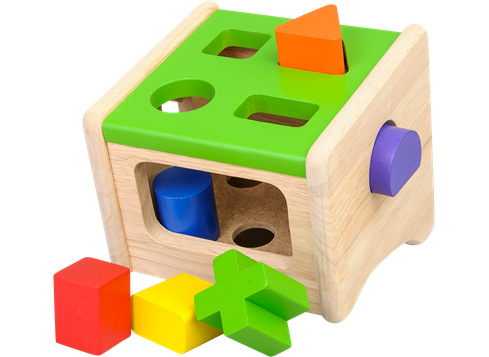
\includegraphics[width=0.8\textwidth]{../img/plocklada.png}
\end{SlideExtra}
\fi


\begin{Slide}{Kolla om det passar med \texttt{match}-uttryck}\SlideFontSmall
I stället för nästlade \code{if} kan du använda Scalas kraftfulla \code{match}-\Emph{uttryck}:

\begin{Code}
def g = scala.io.StdIn.readLine("Ange en grönsak: ")
def smak = g match 
  case "gurka"    => "gott!"
  case "tomat"    => "jättegott!"
  case "broccoli" => "ganska gott..."
  case _ => "mindre gott..."
\end{Code}
\begin{itemize}
\pause\item Varje \code{case}-gren testas var för sig i tur och ordning uppifrån och ned.
\item Det som står mellan \code{case} och \code{=>} kallas ett \Emph{mönster} \Eng{pattern}
\item Sista default-grenen ovan kallas \Emph{wildcard-mönster}: \code{case _ => }
\item Ovan är exempel på matchning mot \Emph{konstant-mönster}, \\ i detta fallet tre stycken strängkonstantmönster.
\item Det finns många andra sätt att skriva mönster.
\end{itemize}
% \pause Scalas \code{match} ''faller inte igenom'' som \code{switch}-satser som finns i många språk, t.ex. Java...

\end{Slide}


\begin{Slide}{Matchning med gard}
Man kan stoppa in en s.k \Emph{gard} \Eng{guard} innan pilen \code{=>} för att villkora matchningen: (notera \code{if} utan \code{then})
\begin{Code}
def g = scala.io.StdIn.readLine("Ange en grönsak: ")
def smak = g match 
  case "gurka" if math.random() > 0.5 => "gott ibland!"
  case "tomat" => "jättegott!"
  case "broccoli" => "ganska gott..."
  case _ => "mindre gott..."
\end{Code}
\code{case}-grenen med gard ger bara en lyckad matchning \\ om uttrycket efter \code{if} är sant; annars provas nästa gren, etc.
\end{Slide}

\begin{Slide}{Matchning med variabelmönster}\SlideFontSmall
Om det finns ett namn efter \code{case} som börjar med liten begynnelsebokstav, blir detta namn en variabel som automatiskt binds till uttrycket före \code{match}:

\begin{Code}
def g = scala.io.StdIn.readLine("Ange en grönsak: ")
def smak = g match 
  case "gurka" if math.random() > 0.5 => "gott ibland!"
  case "tomat" => "jättegott!"
  case "broccoli" => "ganska gott..."
  case other => "smakar bakvänt: " + other.reverse
\end{Code}

Ett enkelt variabelmönster, så som \\ \code{case other => ...} \\ i exemplet ovan, matchar \Emph{allt}! \\\code{other} får alltså värdet av \code{g} om \code{g} \Alert{inte} är \code{"gurka"}, \code{"tomat"}, \code{"broccoli"}.

\end{Slide}


\begin{Slide}{Matchning med eller-mönster}\SlideFontSmall
Om man har samma utfall för olika grenar kan dessa slås ihop och mönstret separeras med vertikalstreck: \code{|}
\begin{Code}
def g = scala.io.StdIn.readLine("Ange en grönsak: ")
def smak = g match 
  case "gurka" => "gott"
  case "tomat" => "gott"
  case "lök"   => "gott"
  case _ => "inte gott"
\end{Code}

Mer koncist med eller-mönster:

\begin{Code}
def g = scala.io.StdIn.readLine("grönsak:")
def smak = g match 
  case "gurka" | "tomat" | "lök" => "gott"
  case _ => "inte gott"
\end{Code}



\end{Slide}





\begin{Slide}{Matchning med typade mönster}\SlideFontSmall
Med en typannotering efter en variabel får man ett \Emph{typat mönster} \Eng{typed pattern}. Om matchningen lyckas blir värdet \Alert{omvandlat} till den specifika typen och binds till variabeln.
\begin{Code}
def f = 
  if (math.random() < 0.5) 42 + math.random() else "gurka" + math.random()

def g = f match 
  case x: Double => x.round.toInt
  case s: String => s.length
\end{Code}
\code{f} får typen \code{Matchable} som är subtyp till \code{Any}. Vilken typ får \code{g}? \pause ~~\code{Int}\\
Matchning mot specifika typer enl. ovan används i idiomatisk Scala hellre än \code{isInstanceOf} men man kan göra motsvarande ovan med detta if-uttryck:
\begin{Code}
def g2 =  
  val x = f
  val y = 
    if (x.isInstanceOf[Double]) x.asInstanceOf[Double].round.toInt
    else if (x.isInstanceOf[String]) x.asInstanceOf[String].length
  y.asInstanceOf[Int] // kan detta ge körtidsfel? kan kompilatorn kolla det?
\end{Code}
\end{Slide}

\begin{Slide}{Typen \text{Matchable}}
När ett uttryck inte kan ges en mer specifik typ så härleds \code{Matchable}, vilket visar att värdet kan undersökas med \code{match}.\footnote{Mer detaljer om varför \code{Matchable} behövs här: https://dotty.epfl.ch/docs/reference/other-new-features/matchable.html}
\begin{REPLnonum}
scala> def f = if math.random() > 0.5 then 42 else "hej"
def f: Matchable
\end{REPLnonum}
%Eftersom typen \code{String} och typen \code{Double} inte har något annat gemensamt bli den mest specifika typen som kan härledas \code{Matchable}, som är nästan lika generell som topptypen \code{Any}.
\end{Slide}

\begin{Slide}{Konstruktormönster med case-klasser}\SlideFontSmall
En basklass med gemensamma delar och två subtyper:
\begin{Code}
trait Grönsak:
  def vikt: Int
  def ärRutten: Boolean

case class Gurka(vikt: Int, ärRutten: Boolean) extends Grönsak
case class Tomat(vikt: Int, ärRutten: Boolean) extends Grönsak
\end{Code}
\pause
Tack vare case-klasserna kan man använda \Emph{konstruktormönster} \Eng{constructor pattern} för att se vad som finns \Alert{inuti} en instans:
\begin{Code}
def testa(g: Grönsak): String = g match 
  case Gurka(v, false) => "gott, väger " + v
  case Gurka(_, true)  => "inte gott"
  case Tomat(v, r)     => (if r then "inte " else "") + s"gott, väger $v"
  case _ => "okänd grönsak: $g"
\end{Code}

Konstruktormönster ''\Emph{plockar isär}'' det som matchas och binder variabler till de attribut som finns i case-klassens konstruktor.
\end{Slide}


\begin{Slide}{Plocka isär samlingar med djupa mönster}
Man kan plocka isär innehållet i en samling så här:
\begin{Code}
def visa(xs: Vector[Grönsak]): String = xs match
  case Vector()               => "tom grönsaksvektor"
  case Vector(Gurka(v, true)) => s"en rutten gurka som väger $v"
  case Vector(g)              => s"exakt en grönsak: $g"
  case Vector(g1, g2)         => s"exakt två grönsaker: $g1, $g2"
  case g +: gs                => s"först en $g och sedan svansen: $gs"
\end{Code}
Vad händer om du byter ordning på andra och tredje mönstret?
\end{Slide}

\begin{Slide}{Matchning på tupler}
Det går fint att plocka isär tupler med mönstermatchning:\footnote{\url{https://youtu.be/aboZctrHfK8}}
\begin{Code}
var pair = ("hej", 42)

pair match
  case (a, b) if b == 42 => s"livets mening är funnen: $a"
  case (_, b)            => s"fattas mening: $b"

\end{Code}

\end{Slide}

\begin{Slide}{Mönstermatchning och uppräkning med case-objekt}\SlideFontSmall
En bastyp och specifika singelobjekt av gemensam typ:
\begin{Code}
trait Färg
case object Spader  extends Färg // funkar utan case men vi vill ha najs toString
case object Hjärter extends Färg
case object Ruter   extends Färg
case object Klöver  extends Färg

def parallellFärg(f: Färg): Färg = f match
  case Spader  => Klöver
  case Klöver  => Spader
  case Hjärter => Ruter
\end{Code}
Vilken case-gren har vi glömt? Kan kompilatorn hjälpa oss?
\pause
\begin{REPL}
scala> parallellFärg(Ruter)
scala.MatchError: Ruter 
\end{REPL}
\Alert{Undantag vid körtid} \code{:(}
\end{Slide}

\begin{Slide}{Mönstermatchning och förseglade typer}\SlideFontSmall
Med nyckelordet \code{sealed} får vi en kompileringsvarning.
\begin{Code}
sealed trait Färg //tryck Alt+Enter i REPL för tolkning av flera rader ett svep
case object Spader  extends Färg
case object Hjärter extends Färg
case object Ruter   extends Färg
case object Klöver  extends Färg

def parallellFärg(f: Färg): Färg = f match 
  case Spader  => Klöver
  case Klöver  => Spader
  case Hjärter => Ruter
\end{Code}
\begin{REPL}
1 |def parallellFärg(f: Färg): Färg = f match 
  |                                   ^
  |                           match may not be exhaustive.
  |
  |                           It would fail on pattern case: Ruter
def parallellFärg(f: Färg): Färg
\end{REPL}
\Emph{Varning vid kompilering} \code{:)} ~~~Sista raden visar att det bara är en varning!
\end{Slide}

\begin{Slide}{Mönstermatcha enumeration}\SlideFontSmall
I stället för \code{sealed trait ... case object ...} kan du använda en \Emph{enumeration} (ä.k. uppräkning, uppräknad datatyp, \Eng{enumeration}).
\begin{Code}
enum Färg:
  case Spader, Hjärter, Ruter, Klöver
  
def parallellFärg(f: Färg): Färg = 
  import Färg.*
  f match 
    case Spader  => Klöver
    case Klöver  => Spader
    case Hjärter => Ruter
\end{Code}
\pause
\begin{REPL}
def parallellFärg(f: Färg): Färg
3 |  f match 
  |  ^
  |  match may not be exhaustive.
  |
  |  It would fail on pattern case: Ruter
\end{REPL}
\Emph{Även här får vi hjälpsam varning vid kompilering} \code{:)} 
\end{Slide}

\begin{Slide}{Stora/små begynnelsebokstäver vid matchning}
\Alert{Fallgrop}: matcha \Alert{värde} som börjar med \Alert{liten} bokstav.
\begin{REPL}
scala> val livetsMening = 42

scala> def ärLivetsMeningBuggig(svar: Int) = svar match 
         case livetsMening => true    // lokalt namn som matchar allt!
         case _ => false

scala> ärLivetsMeningBuggig(43)
val res0: Boolean = true

scala> val LivetsMening = 42   // stor begynnelsebokstav

scala> def ärLivetsMening(svar: Int) = svar match 
         case LivetsMening => true    // funkar fint!
         case _ => false

scala> ärLivetsMening(43)
val res1: Boolean = false
\end{REPL}
\end{Slide}


\begin{Slide}{Stora/små begynnelsebokstäver vid matchning}
Ett sätt att komma runt problemet med liten begynnelsebokstav: \\
\Emph{backticks} to the rescue!
\begin{REPL}
scala> val livetsMening = 42

scala> def ärLivetsMeningBackTicks(svar: Int) = svar match 
         case `livetsMening` => true    // nu funkar det!
         case _ => false

scala> ärLivetsMeningBackTicks(43)
val res2: Boolean = false
\end{REPL}
\end{Slide}


\begin{Slide}{Mönster på andra ställen än i \texttt{match}}\SlideFontSmall
Mönster i \Emph{deklarationer}:
\vspace{-0.25em}\begin{REPL}
scala> case class Point(x: Int, y: Int)

scala> val p = Point(0, 1)

scala> val Point(x, y) = p          // konstruktormönster med case-klass
val x: ???
val y: ???

scala> val (x, y, z) = (0, 1, 2)    // konstruktormönster med tupel
val x: ???
val y: ???
val z: ???

\end{REPL}
Mönster i \Emph{for-satser}:
\vspace{-0.25em}\begin{REPL}
scala> val xs = for (x, y) <- Vector((1,2), (3,4)) yield x
val xs: ???
\end{REPL}

\end{Slide}

\begin{Slide}{Mönster på andra ställen än i \texttt{match}}\SlideFontSmall
Mönster i \Emph{deklarationer}:
\vspace{-0.25em}\begin{REPL}
scala> case class Point(x: Int, y: Int)

scala> val p = Point(0, 1)

scala> val Point(x, y) = p          // konstruktormönster med case-klass
val x: Int = 0
val y: Int = 1

scala> val (x, y, z) = (0, 1, 2)    // konstruktormönster med tupel
val x: Int = 0
val y: Int = 1
val z: Int = 2

\end{REPL}
Mönster i \Emph{for-satser}:
\vspace{-0.25em}\begin{REPL}
scala> val xs = for (x, y) <- Vector((1,2), (3,4)) yield x
val xs: Vector[Int] = Vector(1, 3)
\end{REPL}
\end{Slide}

\begin{Slide}{Fördjupning om mönster}\SlideFontSmall
\begin{itemize}
\item binda variabler till mönsterdelar med \code{@} \\
\code{case Vector(xs@Vector(a), Vector(42)) => ...}

\item sekvensmönster med \code{_}, \code{xs*} och \code{_*} 
\\ \code{case Vector(a, _, c) => ... }  matchar om 3 element, \_ kvittar
\\ \code{case Vector(a, svans*) => ... }  matchar om minst ett element
\\ \code{case Vector(a, _*) => ... }  intresserad av första, svans kvittar

\item Partiella funktioner med \code{case} utan \code{match}: \code|val pf: Int => Double = { case z if z != 0 => 1/z }| \\ Notera att klammerparenteserna behövs för att skapa partiell funktion med \code{case} utan \code{match}. Funktionen är inte definierad för argumentet \code{0}:

\begin{REPLsmall}
scala> pf(0)                         
scala.MatchError: 0 
\end{REPLsmall}
Detta är användbart vid iterering över samling med \code{collect}: \\\code|xs.collect{ case (a,b) if a > 0 => a }|  
\item Läs mer om mönster här: \\\url{https://docs.scala-lang.org/scala3/book/control-structures.html}

% \item Läs mer om mönster här:  \href{http://www.artima.com/pins1ed/case-classes-and-pattern-matching.html}{\SlideFontTiny www.artima.com/pins1ed/case-classes-and-pattern-matching.html}

% \item För djupare förståelse av hur \code{case} fungerar, läs speciellt om \Emph{partiella funktioner} här: \href{http://www.artima.com/pins1ed/case-classes-and-pattern-matching.html\#15.7}{\SlideFontTiny www.artima.com/pins1ed/case-classes-and-pattern-matching.html\#15.7}

% \item Läs om extractors här: \href{http://www.artima.com/pins1ed/extractors.html}{\SlideFontTiny www.artima.com/pins1ed/extractors.html}

\end{itemize}
\end{Slide}


\begin{Slide}{Fördjupning: metoden \texttt{unapply}}\SlideFontSmall
När du deklarerar en case-klass kommer kompilatorn att \Alert{automatiskt generera en metod} med namnet \Emph{\texttt{unapply}}.
\begin{REPL}
scala> case class Gurka(vikt: Int, ärRutten: Boolean)

scala> Gurka.unapply // tryck ENTER för att se typen
val res0: Gurka => Gurka = Lambda1914/0x00000008408cf840@b0e7bde

scala> val g = Gurka(100, false)

scala> Gurka.unapply(g)
val res1: Gurka = Gurka(100,false)
\end{REPL}
Vad ska detta vara bra för? \\\pause
\code{unapply} genereras av kompilatorn och används internt vid matchning och det är den metoden som gör att case-klasser kan användas i konstruktormönster. \\Principen är generell: Man kan skapa \Emph{egna} s.k. \Alert{extraktorer} \Eng{extractors} som kan plocka isär ett värde med mönstermatchning, genom att definiera en egen \code{unapply}.
\end{Slide}

%!TEX encoding = UTF-8 Unicode
%!TEX root = ../lect-w06.tex

%%%


\ifkompendium\else
%\Subsection{Kapsla in speciella värden: Option[kanske saknas] och Try[kanske misslyckas]}
\Subsection{Hantera speciella värden med inkapsling}

{
\setbeamertemplate{navigation symbols}{}
\setbeamercolor{background canvas}{bg=black}
\begin{frame}[plain]
    \color{white}{Inkapsling av speciella värden så att krasch kan undvikas}
    \makebox[\linewidth]{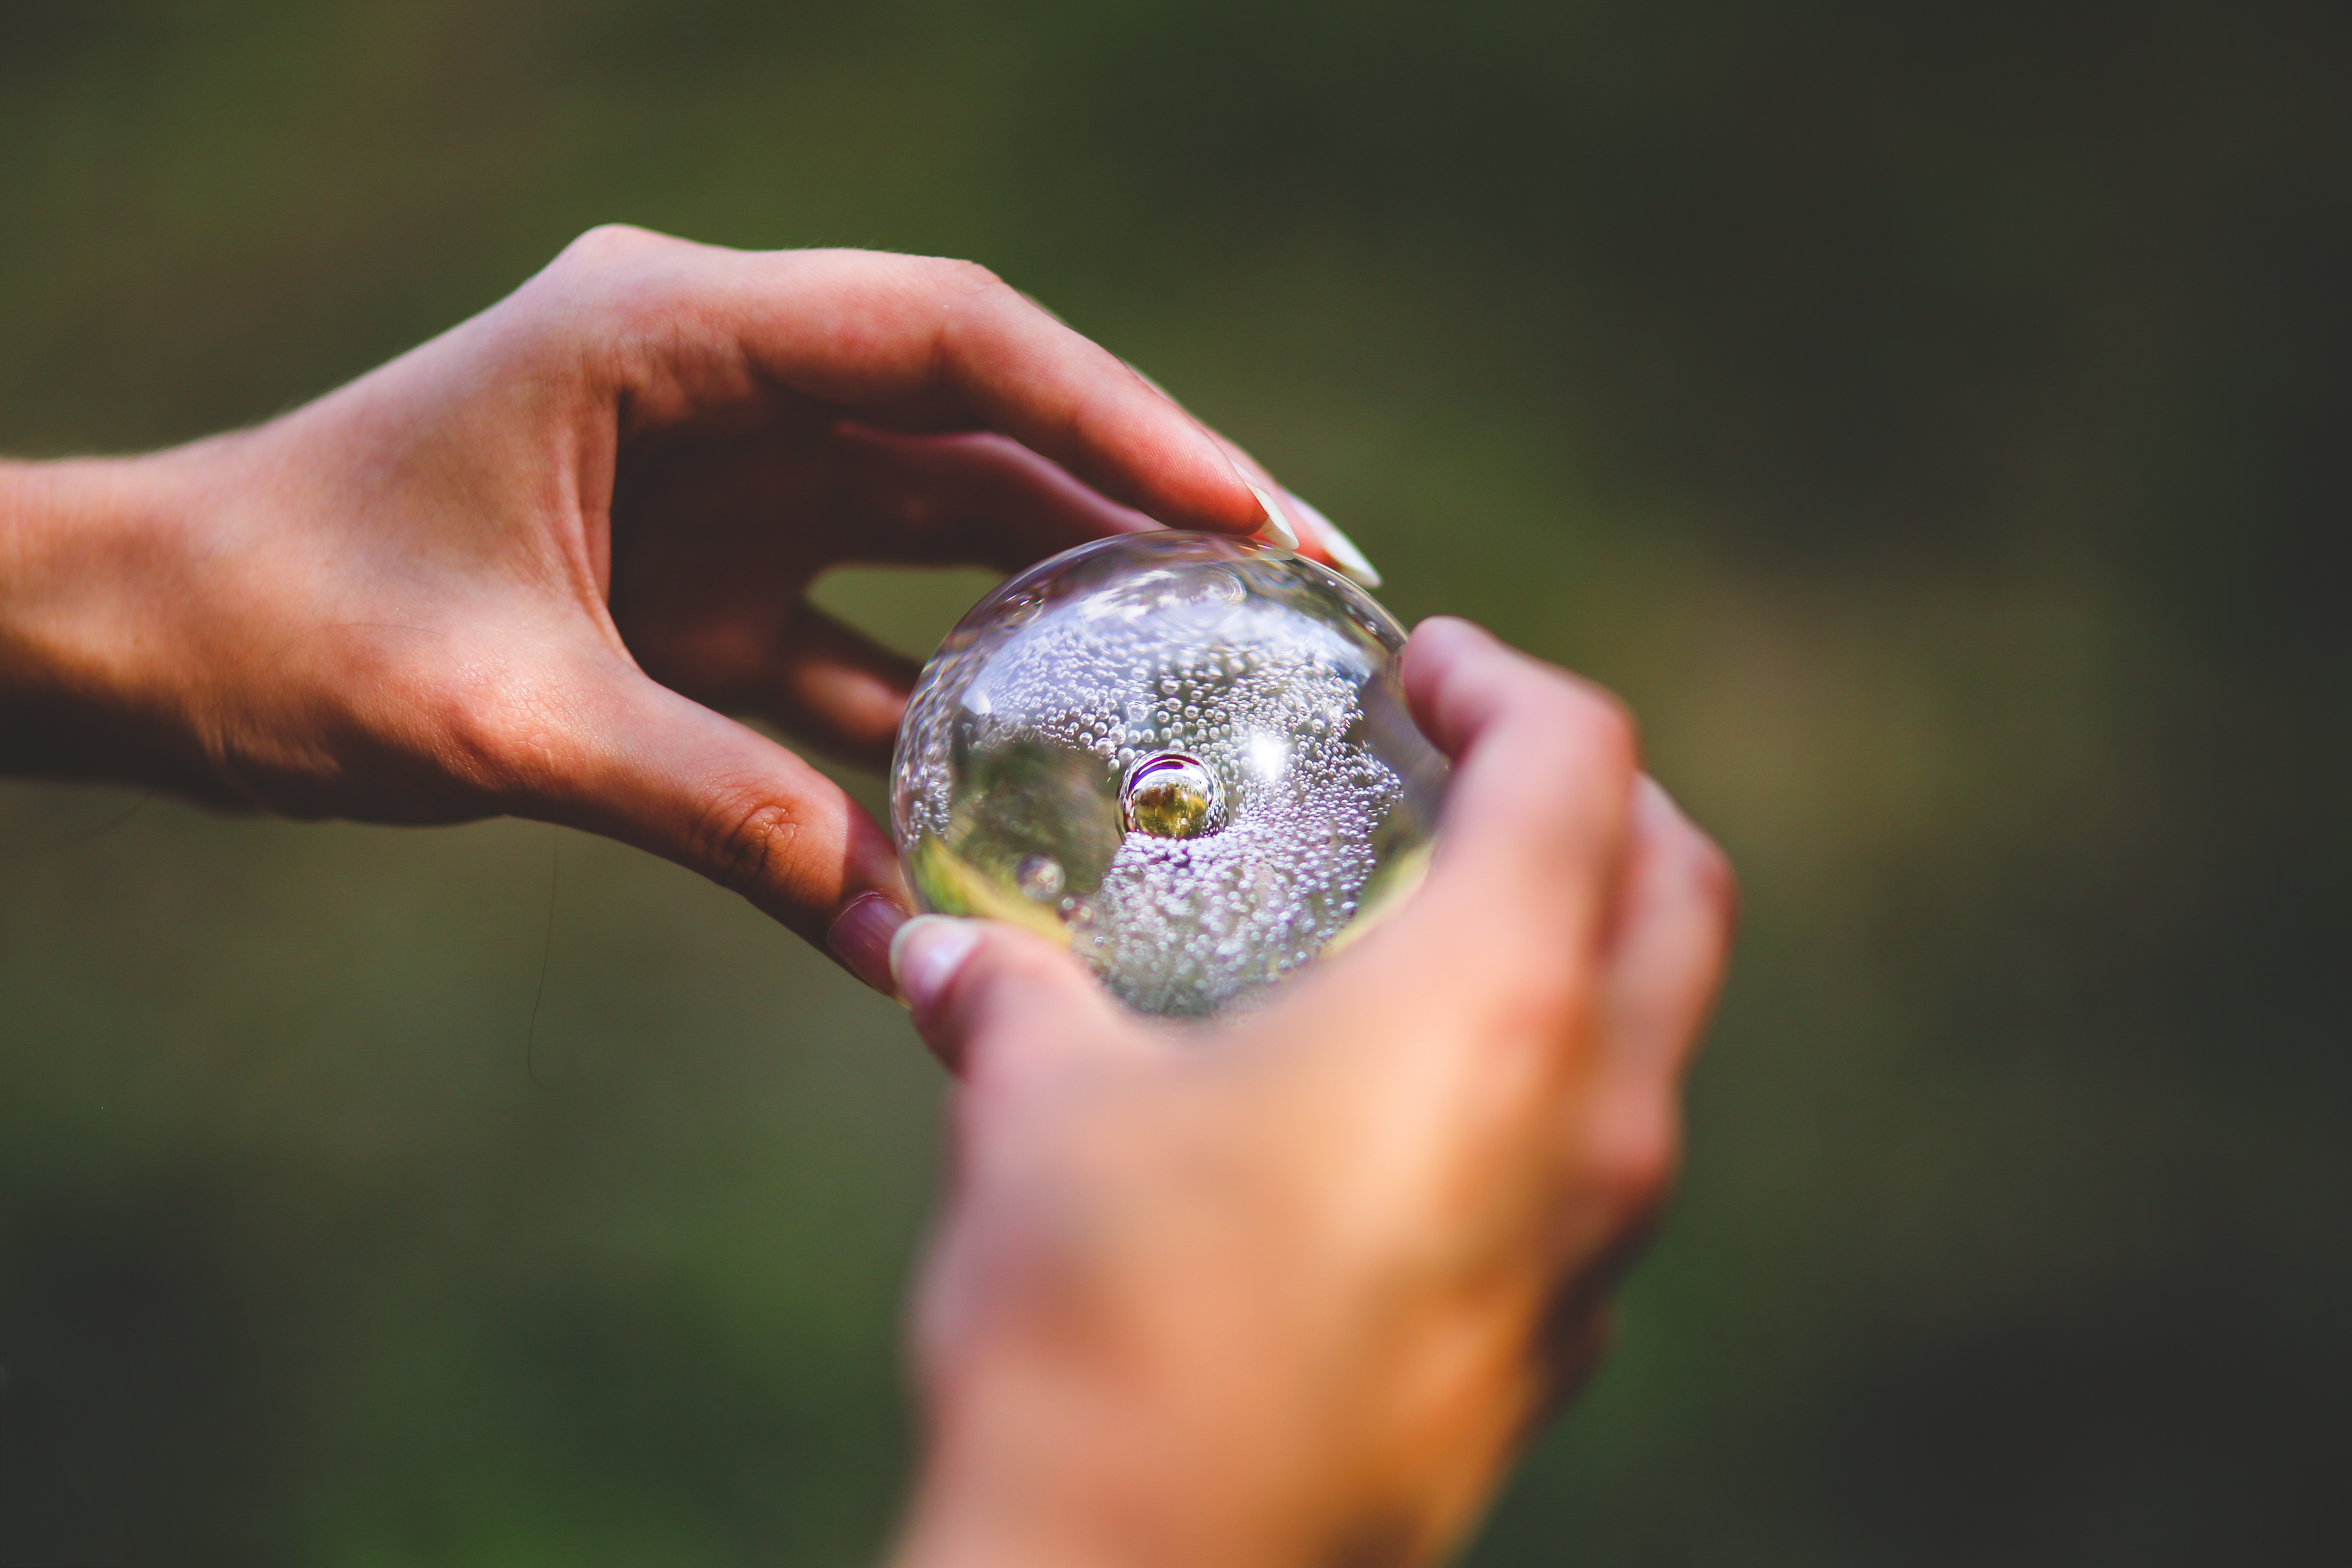
\includegraphics[width=\paperwidth]{../img/crystal.jpg}}
\end{frame}
}
\fi

\Subsection{Hantera saknade värden med \texttt{Option}}

\begin{Slide}{Hur hantera saknade värden?}\SlideFontSmall
Olika sätt att hantera saknade värden:
\begin{itemize}
\item Hitta på ett specialvärde: exempel -1 för saknat värde
\item \code{null} om värde saknas (vanligt i Java m.fl. språk, mkt ovanligt i Scala)
\item Använd en samling och låt tom samling representera saknat värde: \\
\code{val sums = Vector(Vector(42),Vector(32),Vector(),Vector(21))}

\item \code{Option[A]} gemensam bastyp för: \\
  \code{None} som representerar \Alert{saknat värde}, och \\ \code{Some[A]} som representerar att \Emph{värde finns}
\end{itemize}
\end{Slide}



\begin{Slide}{En gemensam bastyp för ett värde som kanske saknas}\SlideFontSmall\ifkompendium\footnotesize\fi
\vspace{-0.0em}\begin{center}
\newcommand{\TextBox}[1]{\raisebox{0pt}[1em][0.5em]{#1}}
\tikzstyle{umlclass}=[rectangle, draw=black,  thick, anchor=north, text width=3cm, rectangle split, rectangle split parts = 3]
\begin{tikzpicture}[inner sep=0.5em]
\node [umlclass, rectangle split parts = 2, xshift=0cm, text width=3.5cm] (BaseType)  {
            \textit{\textbf{\centerline{\TextBox{\code{Option[A]}}}}}
            \nodepart[]{second}
            \TextBox{\code{def get: A}}\newline
            \TextBox{\code{def isEmpty: Boolean}}

        };

\node [umlclass, rectangle split parts = 1]  at (-2.5cm,-3.0cm) (SubType1) {
            \textbf{\centerline{\TextBox{\code{Some[A]}}}}
            % \nodepart[]{second} \TextBox{\code{val x: A}}
        };

\node [umlclass, rectangle split parts = 1] at (2.5cm,-3.0cm) (SubType2)  {
            \textbf{\centerline{\TextBox{\code{None}}}}
        };
\draw[umlarrow] (SubType1.north) -- ++(0,0.5) -| (BaseType.south);
\draw[umlarrow] (SubType2.north) -- ++(0,0.5) -| (BaseType.south);
\end{tikzpicture}
\end{center}
\pause
\vspace{-0.5em}\begin{REPL}
scala> var x: Option[Int] = Some(42)

scala> x.isEmpty
val res0: Boolean = false

scala> x = None

scala> x.isEmpty
val res1: Boolean = true
\end{REPL}
\end{Slide}


\begin{Slide}{Option för hantering av ev. saknade värden}\SlideFontSmall
Alla vill inte berätta för Facebook vad de har för kön. \\ Förbättra Facebooks kod med ett litet Scala-program:
\begin{Code}
enum Gender:
  case Male, Female

case class Person(name: String, gender: Option[Gender])
\end{Code}
\pause
\begin{REPL}
scala> val p1 = Person("Björn",  Some(Gender.Male))
scala> val p2 = Person("Sandra", Some(Gender.Female))
scala> val p3 = Person("Kim",  None)
scala> val g2 = p2.gender
scala> def show(g: Option[Gender]): String = g match {
         case Some(x) => x.toString
         case None    => "unknown"
       }
scala> show(g2)
scala> show(p3.gender)
scala> val ps = Vector(p1,p2,p3)
scala> ps.map(_.gender).map(show)   // None ignoreras av map
\end{REPL}
\end{Slide}

\begin{Slide}{Några smidiga metoder på \code{Option}}\SlideFontSmall
Metoden \code{getOrElse} gör att man ofta kan undvika matchning.
\begin{Code}
var opt: Option[Int] = None

val x = opt.getOrElse(42)      // get the value or give a default if missing
\end{Code}

Flera av de vanliga samlingsmetoderna funkar, t.ex. \code{foreach} och \code{map}.
\begin{Code}
opt.foreach{x => println(x)}    // only done if value exists

opt.map{x => x + 1}             // only done if value exists

opt = Some(42)                  // change opt to now have some value

opt.foreach{x => println(x)}    // done as value now exists

opt.map{x => x + 1}             // done as value now exists

\end{Code}
\end{Slide}


\begin{Slide}{Några samlingsmetoder som ger en \code{Option}, övning}
\begin{REPL}
scala> val (xs, ys) = (Vector(1,2,3), Vector())

scala> xs.headOption
res0: ???

scala> ys.headOption
res1: ???

scala> xs.find(_ > 1)
res2: ???

scala> xs.find(_ > 5)
res3: ???

scala> val huvudstad = Map("Sverige" -> "Sthlm", "Skåne" -> "Malmö")

scala> huvudstad.get("Skåne")
res4: ???

scala> huvudstad.get("Danmark")
res5: ???
\end{REPL}
\end{Slide}

\begin{Slide}{Några samlingsmetoder som ger en \code{Option}, svar}
\begin{REPL}
scala> val (xs, ys) = (Vector(1,2,3), Vector())

scala> xs.headOption
res0: Option[Int] = Some(1)

scala> ys.headOption
res1: Option[Nothing] = None

scala> xs.find(_ > 1)
res2: Option[Int] = Some(2)

scala> xs.find(_ > 5)
res3: Option[Int] = None

scala> val huvudstad = Map("Sverige" -> "Sthlm", "Skåne" -> "Malmö")

scala> huvudstad.get("Skåne")
res4: Option[String] = Some(Malmö)

scala> huvudstad.get("Danmark")
res5: Option[String] = None
\end{REPL}
\end{Slide}

%!TEX encoding = UTF-8 Unicode
%!TEX root = ../lect-w06.tex

%%%



\Subsection{Undantag}

\ifkompendium\else
\begin{SlideExtra}{Undantag kan orsaka krasch...}
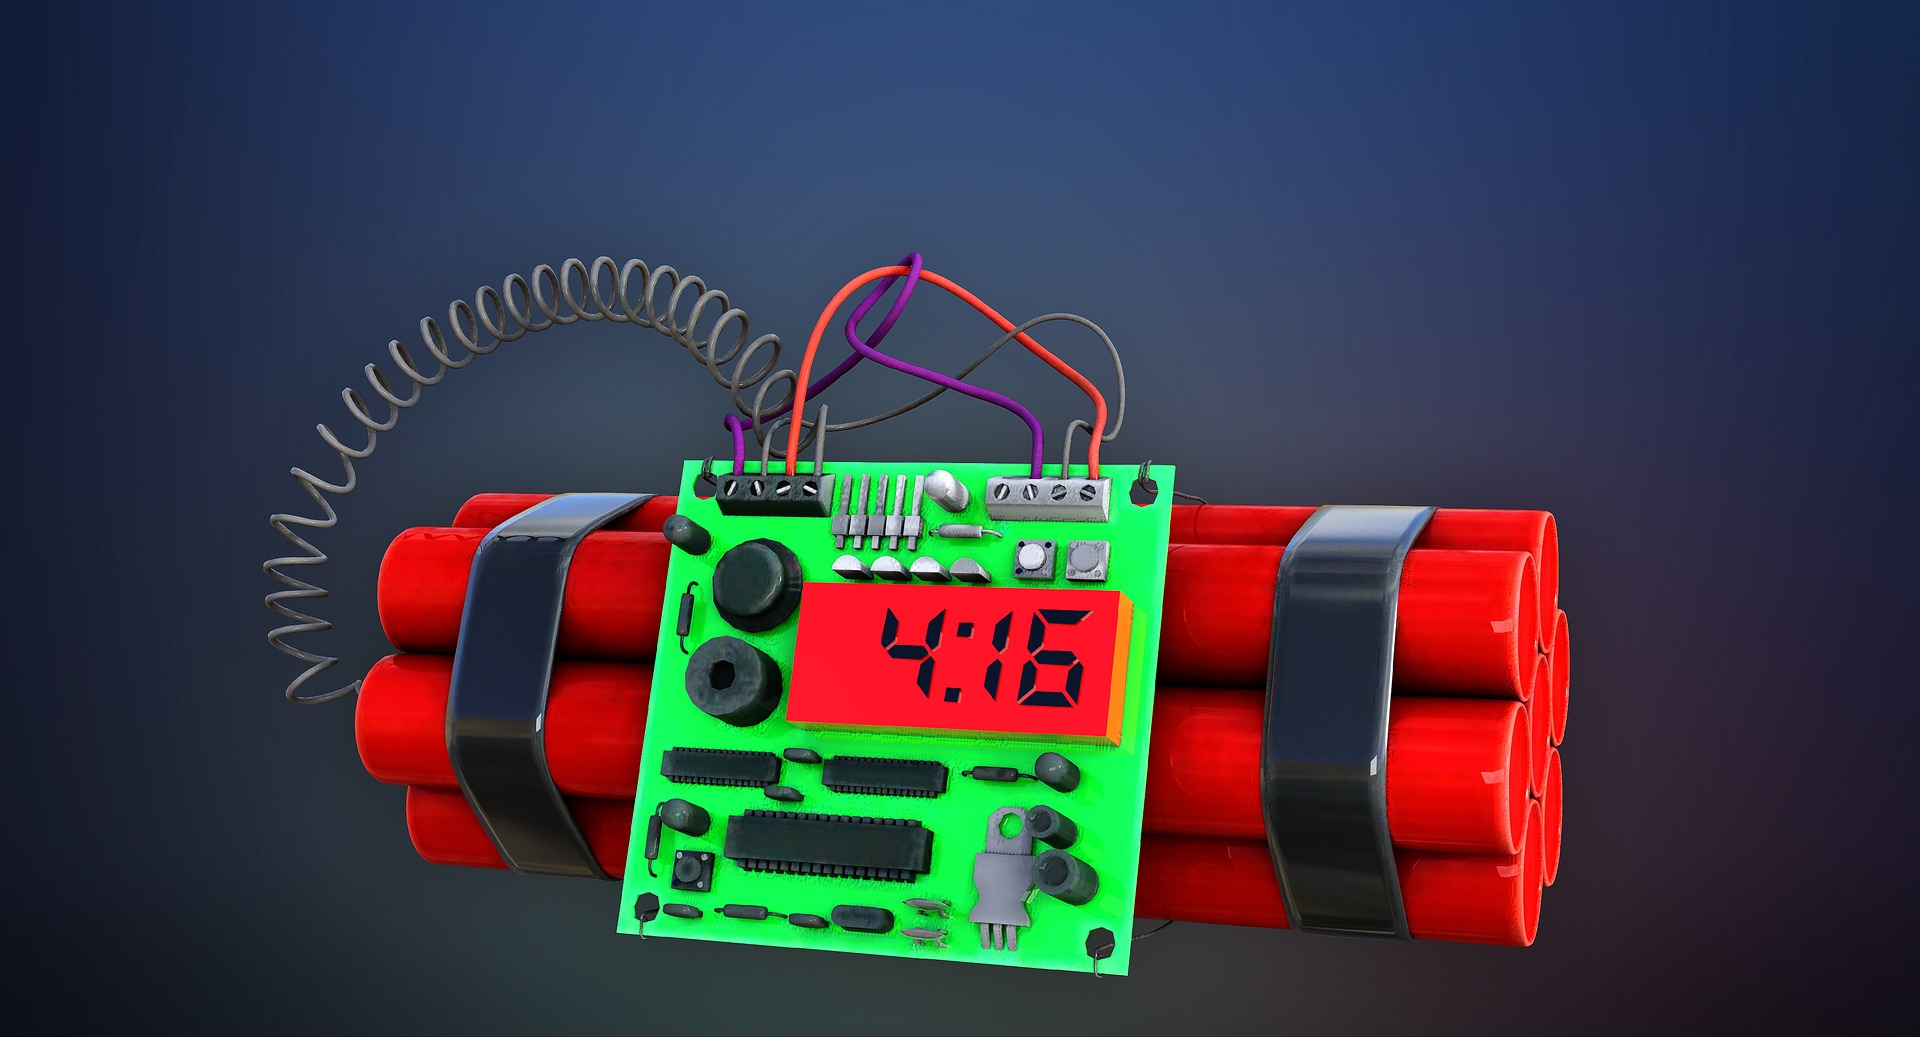
\includegraphics[width=1.0\textwidth]{../img/dynamite}  
\end{SlideExtra}

\begin{SlideExtra}{Undantag orsakar ingen krasch om inkapslad i en Try}
\hspace{0.3\textwidth}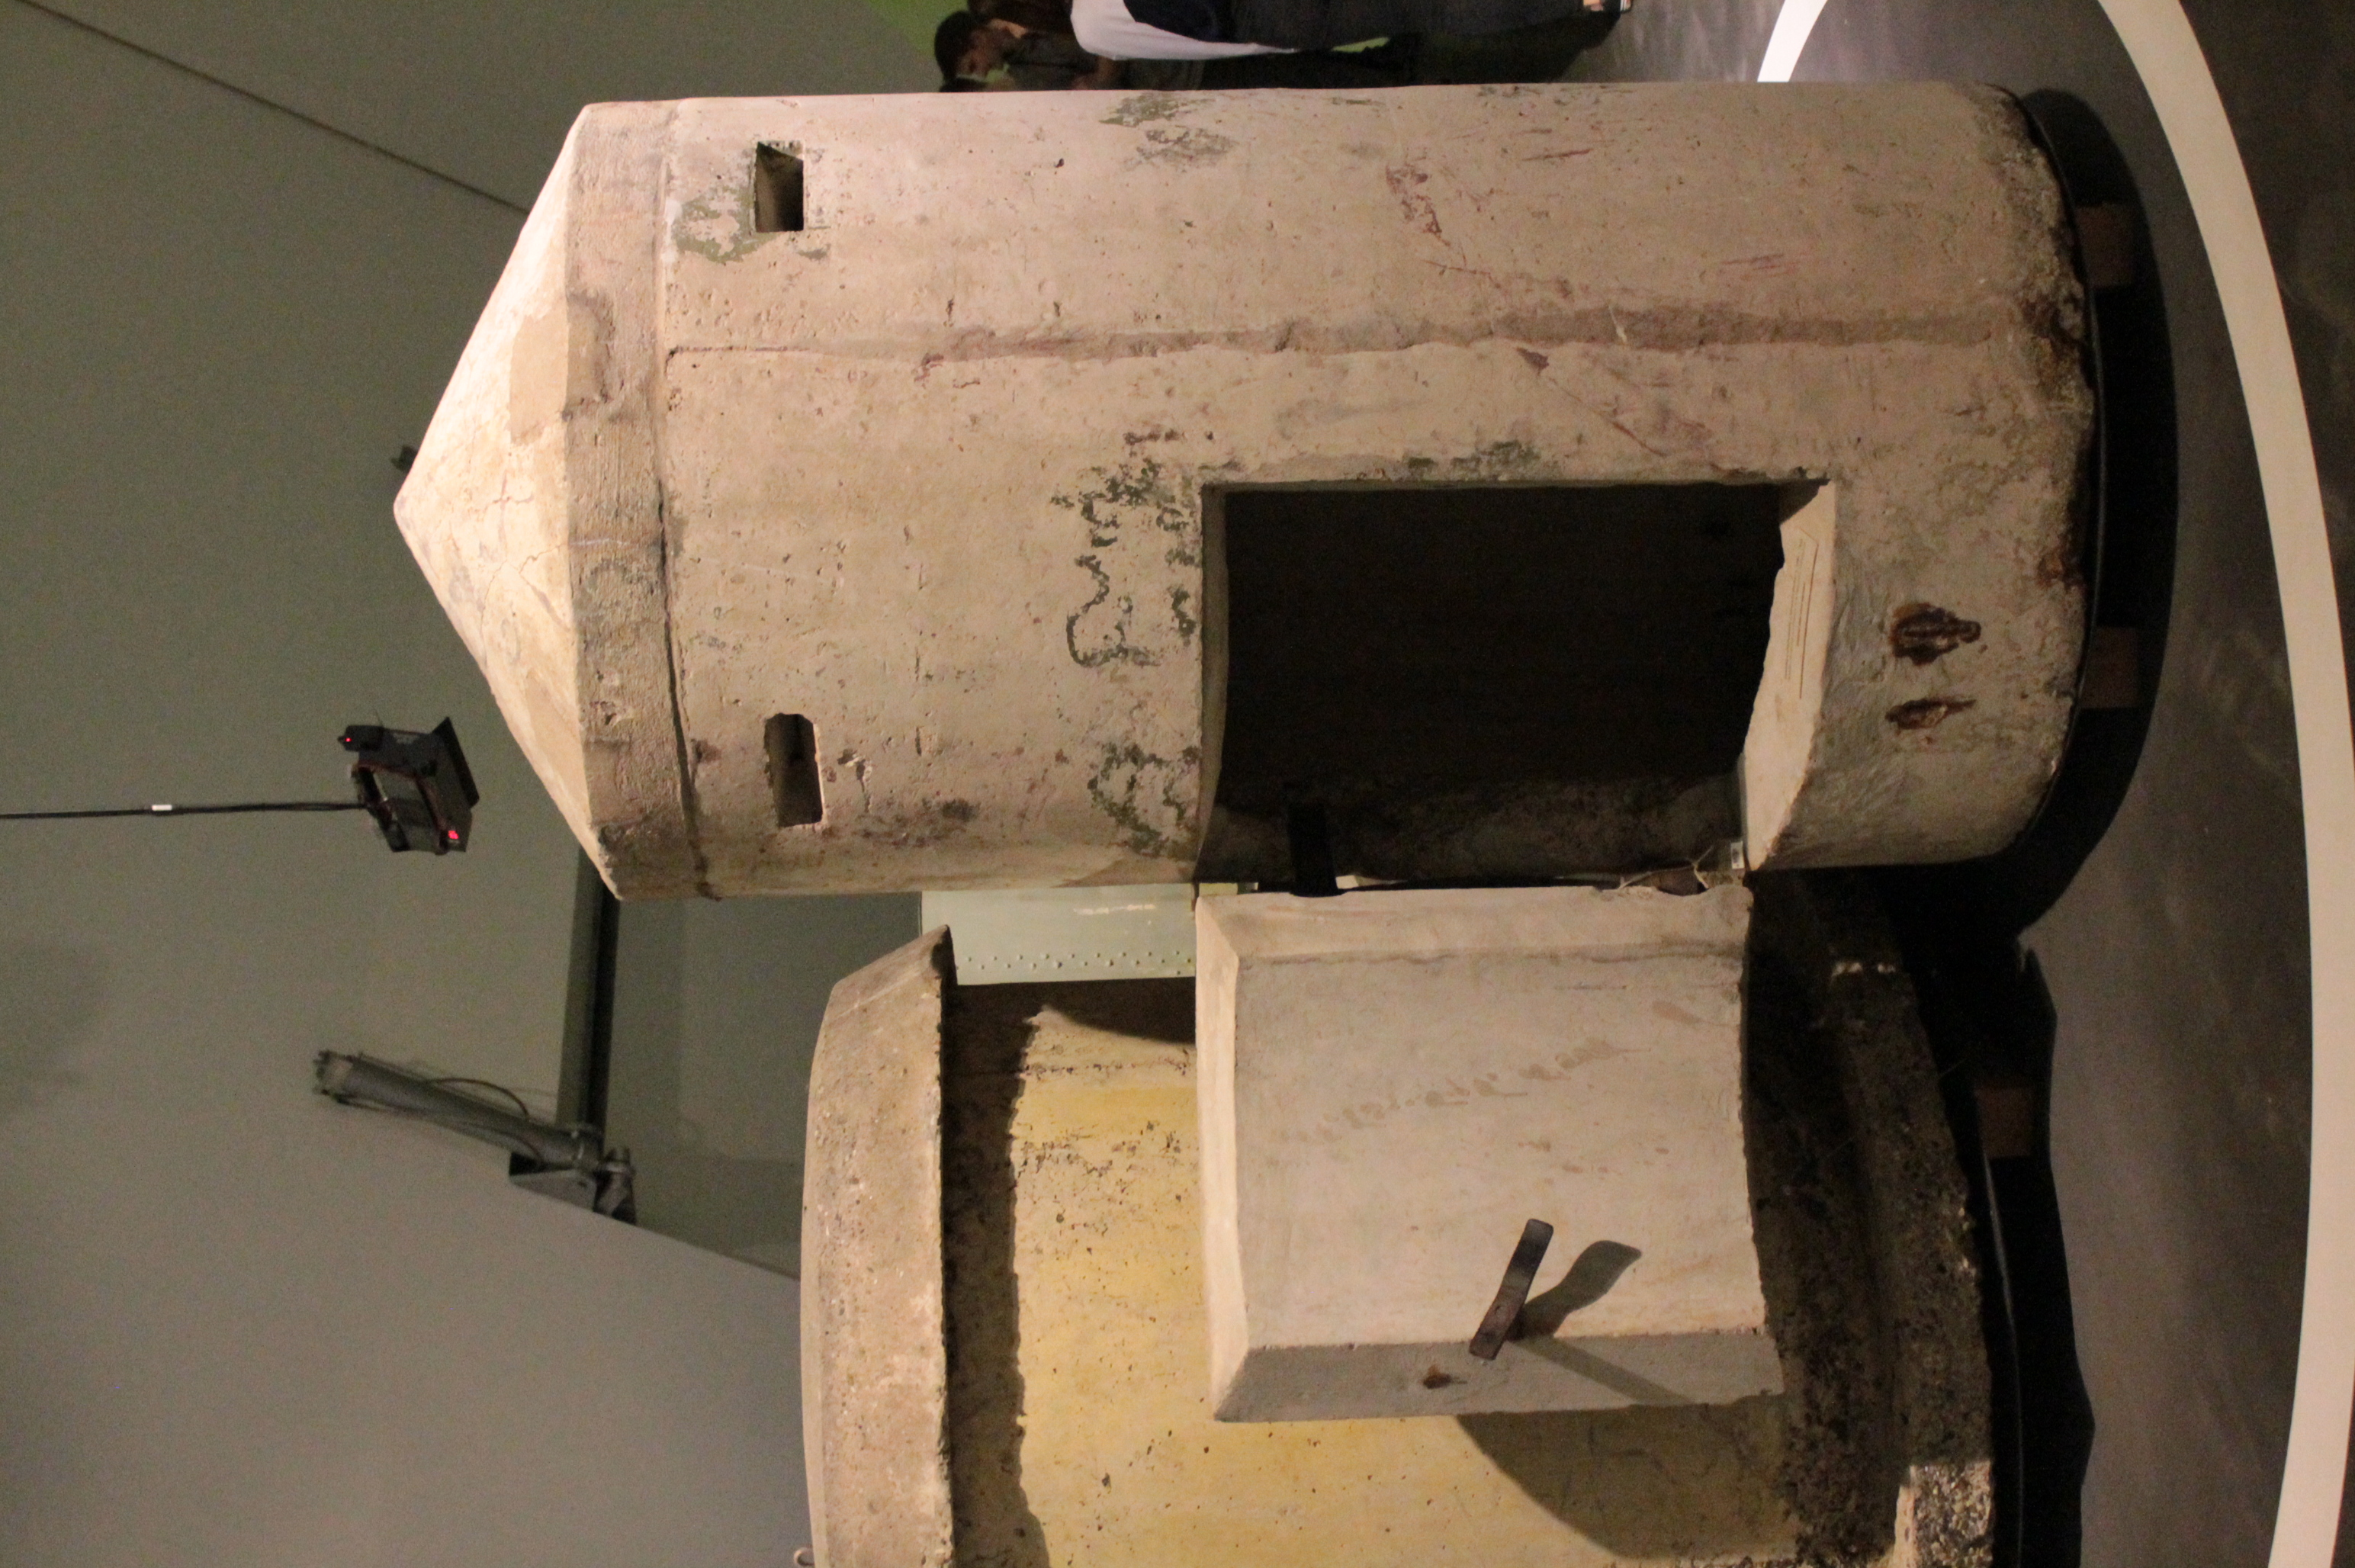
\includegraphics[width=0.6\textwidth,angle=-90,origin=c]{../img/bomb-shelter}  
\end{SlideExtra}
\fi

\begin{Slide}{Vad är ett undantag \Eng{exception}?}
Undantag representerar ett fel eller ett onormalt tillstånd som upptäcks under exekvering och som  behöver hanteras på särskilt sätt vid sidan av det normala exekveringsflödet.

\vspace{1em}\href{https://sv.wikipedia.org/wiki/Undantagshantering}{sv.wikipedia.org/wiki/Undantagshantering}


\vspace{1em} Exempel på undantag:

\pause

\begin{itemize} \SlideFontSmall
\item Indexering utanför vektorns indexgränser.

\item Läsning bortom filens slut.

\item Försök att öppna en fil som inte finns.

\item Minnet är slut.

\item Heltalsdivision med noll ger \code{java.lang.ArithmeticException}.

\item \code{"hej".toInt} ger \code{java.lang.NumberFormatException}

\end{itemize}

\end{Slide}


\begin{Slide}{Orsaka undantag indirekt med \texttt{require} och \texttt{assert}}

\begin{itemize}\SlideFontSmall
  \item Med funktionen \code{require(p)} skapas ett \\\code{IllegalArgumentException("requirement failed")} \\ om \code{p} är \code{false}
  \item \code{require} används om man vill begränsa vilka argument som är giltiga
  \item Med funktionen \code{assert(p)} skapas ett \code{AssertionError("assertion failed")} \\ om \code{p} är \code{false} 
  \item \code{assert} används om man vill förhindra ogiltiga tillstånd
\end{itemize}
{
  \ifkompendium\else
  \vfill\SlideFontTiny
  \fi
  Se implementationen av \code{require} här:\\
\url{https://github.com/scala/scala/blob/v2.13.6/src/library/scala/Predef.scala#L315}
}
\end{Slide}

\begin{Slide}{Kasta dina egna undantag med \texttt{throw}}\SlideFontSmall
Man kan själv generera ett undantag med \code{throw}, vilket kallas att \Emph{kasta} ett undantag som (om det inte \Emph{fångas}), gör att exekveringen \Alert{avbryts}.


\begin{REPL}
scala> def pang = throw Exception("PANG!")
pang: Nothing

scala> pang
java.lang.Exception: PANG!

\end{REPL}
\pause
Olika sätt att hantera undantag och förhindra att exekveringen avbryts:
\begin{itemize}
\item \code{try catch}-uttryck omvandlar undantag till ngt lämpligt värde.
%\item Java: Man kan använda en \code{try ... catch}-sats och \Alert{göra något} i händelse av undantag.

\item \texttt{scala.util.Try} \Emph{kapslar in} kod som kan ge undantag.  %(Finns ej i Java; att föredra i Scala.)
\end{itemize}
\end{Slide}


\Subsection{Hantera undantag med \texttt{Try}}

\begin{Slide}{En gemensam bastyp för något som kan misslyckas}\SlideFontSmall
\begin{Code}
import scala.util.{Try, Success, Failure}
\end{Code}
\ifkompendium\footnotesize\fi
\vspace{-0.5em}\begin{center}
\newcommand{\TextBox}[1]{\raisebox{0pt}[1em][0.5em]{#1}}
\tikzstyle{umlclass}=[rectangle, draw=black,  thick, anchor=north, text width=3.0cm, rectangle split, rectangle split parts = 3]
\begin{tikzpicture}[inner sep=0.5em]
\node [umlclass, rectangle split parts = 2, xshift=0cm, text width=3.8cm] (BaseType)  {
            \textit{\textbf{\centerline{\TextBox{\code{Try[T]}}}}}
            \nodepart[]{second}
            \TextBox{\code{def get: T}}\newline
            \TextBox{\code{def isFailure: Boolean}}\newline
            \TextBox{\code{def isSuccess: Boolean}}
        };

\node [umlclass, rectangle split parts = 2, text width=2.2cm]  at (-2.5cm,-3.7cm) (SubType1) {
            \textbf{\centerline{\TextBox{\code{Success[T]}}}}
            \nodepart[]{second} \TextBox{\code{val value: T}}
        };

\node [umlclass, rectangle split parts = 2, text width=4.2cm] at (2.5cm,-3.7cm) (SubType2)  {
            \textbf{\centerline{\TextBox{\code{Failure[T]}}}}
            \nodepart[]{second} \TextBox{\code{val exception: Throwable}}
        };
\draw[umlarrow] (SubType1.north) -- ++(0,0.5) -| (BaseType.south);
\draw[umlarrow] (SubType2.north) -- ++(0,0.5) -| (BaseType.south);
\end{tikzpicture}
\end{center}
\end{Slide}

\begin{Slide}{Hantera undantag med \texttt{Try}}
\vspace{-0.5em}\begin{REPLsmall}
scala> def pang = throw new Exception("PANG!")

scala> def kanskePang = if math.random() < 0.5 then 42 else pang

scala> import scala.util.{Try, Success, Failure}

scala> def försök = Try { kanskePang }

scala> val xs = Vector.fill(15){försök}

scala> val trettonde = xs(12) match
         case Success(value) => value
         case Failure(e) => println(e); -1

scala> (xs(12).isSuccess, xs(12).isFailure) 

scala> xs(12).getOrElse(0)

scala> xs(12).toOption

scala> försök.foreach(println)

scala> försök.map(_ + 1)

scala> for Success(x) <- xs yield x
\end{REPLsmall}
\end{Slide}

\Subsection{Hantera undantag med \texttt{try}-\texttt{catch}}


\begin{Slide}{\texttt{try}-\texttt{catch}-uttryck}\SlideFontSmall
Man kan fånga undantag med ett \code{try ... catch}-uttryck:
\begin{Code}
def carola = 
  try 
    if math.random() > 0.5 then throw Exception("stormvind")
    42
  catch 
    case e: Exception =>
      println("Fångad av en " + e.getMessage)
      -1

\end{Code}
\pause
\begin{REPL}
scala> Vector.fill(5)(carola)
Fångad av en stormvind
Fångad av en stormvind
Fångad av en stormvind
val res0: Vector[Int] = Vector(-1, 42, 42, -1, -1)
\end{REPL}
%Gör uppg. 9-11 i övn. \code{patterns} som visar hur man fångar undantag i Scala och Java. 
%Mer om undantag i fortsättningskursen.
\end{Slide}

%!TEX encoding = UTF-8 Unicode
%!TEX root = ../lect-w06.tex

%%%

\Subsection{Fördjupning: Implementera \texttt{equals}}

\ifkompendium
\noindent När du jämför värden med \code{==} anropas metoden \code{equals} som finns för alla typer. Du kan i dina egna klasser överskugga \code{equals} med en din egna definition av vad likhet ska innebära. Då är det lämpligt att använda matchning. Det är dock ett ganska omfattande arbete att implementera en korrekt likhetsjämförelse som fungerar under alla omständigheter. Ett recept för en fullständig implementation av \code{equals} ges i fördjupningen nedan. 
\fi

\begin{Slide}{Fördjupning: Implementera \texttt{equals} med \texttt{match}}
Det visar sig att \Emph{innehållslikhet} är \Alert{förvånansvärt komplicerat} att implementera, speciellt  i samband med arv.
\begin{itemize}\SlideFontSmall
\item Det enklare fallet: Gör fördjupningsuppgift \textit{''Metoden \code{equals}''} och implementera \code{equals} för innehållslikhet utan arv. \\ En bra träning på att använda \code{match}!

\item Svårare: Gör fördjupningsuppgifterna  \textit{''Överskugga \code{equals}''} och \textit{''Överskugga equals vid arv''} om du vill se hur en \Emph{komplett} \code{equals} ska se ut som fungerar \Alert{i alla lägen}.

\end{itemize}

\noindent Det krävs i denna kurs inte att du själv ska kunna implementera en generellt fungerande \code{equals}. Men du ska förstå skillnaden mellan referenslikhet och innehållslikhet. Mer om \code{equals} i fortsättningkursen, men en liten inblick i problemet nu...
\end{Slide}

\ifkompendium
\noindent Om en klass markeras \code{final} kan den ej ha några subklasser. Kompilatorn kontrollerar att detta gäller alla finala klasser och ger kompileringsfel om du försöker göra \code{extends} på en final klass. Om en klass garanterat inte har några subklasser kan implementationen av \code{equals} göra enklare.
\fi 

\begin{Slide}{Fördjupning: \texttt{equals} som fungerar för finala klasser}
Recept för implementation av \code{equals} som fungerar för typer som \Alert{inte} har några subtyper:
\begin{Code}
final class Gurka(val vikt: Int, val ärÄtbar: Boolean):
  override def equals(other: Any): Boolean = other match
    case that: Gurka => vikt == that.vikt && ärÄtbar == that.ärÄtbar
    case _ => false

  override def hashCode: Int = (vikt, ärÄtbar).## // ger bra hashcode
\end{Code}
\begin{itemize}\SlideFontSmall
\item
Du \Alert{måste} alltid överskugga \code{hashCode} också om du överskuggar \code{equals} annars funkar inte gurksamlingar (lång story ...)
\item
Notera typen \code{Any} -- detta följer hur man valde att göra i Java (tyvärr?).
\pause
\item
Ett \Alert{typsäkrare} innehållslikhetstest som \Emph{garanterat} bara jämför en gurka med en gurka och inget annat:
\begin{Code}
def ===(other: Gurka): Boolean =
  vikt == other.vikt && ärÄtbar == other.ärÄtbar
\end{Code}
\end{itemize}
\end{Slide}


\begin{Slide}{Fördjupning: Recept i 8 steg för arvssäker \code{equals}}\SlideFontTiny
%fungerar även för klasser som inte är \code{final}:
\SlideOnly{\setlength{\leftmargini}{0pt}}
\begin{enumerate}\SlideFontTiny
\item Inför denna metod: \code{ def canEqual(other: Any): Boolean}\\Observera att typen på parametern ska vara \code{Any}. Om subklass behövs \code{override}.

\item Metoden \code{canEqual} ska ge \code{true} om \code{other} är av samma typ som \code{this}, t.ex.: \\\code{override def canEqual(other: Any): Boolean = other.isInstanceOf[Gurka]}

\item Inför metoden \code{equals} och var noga med att parametern har typen \code{Any}: \\ \code{override def equals(other: Any): Boolean}

\item Implementera metoden \code{equals} med ett match-uttryck som börjar så här: \\
\code|other match { ... } |

\item Match-uttrycket ska ha två grenar. Den första grenen ska ha ett typat mönster för den klass som ska jämföras, t.ex.: \\ \code{  case that: Gurka =>}

\item Om du implementerar \code{equals} i den klass som inför \code{canEqual}, börja med: \\ \code{(that canEqual this) &&} \\
och skapa därefter en fortsättning som baseras på innehållet i klassen, t.ex.: \\ \code{this.vikt == that.vikt && this.längd == that.längd} \\
Om du överskuggar equals vill du nog börja med
 \code{super.equals(that) && }

\item Den andra grenen i matchningen ska vara:
\code{case _ => false}

\item Överskugga \code{hashCode}, t.ex. med tupel av attributvärden och metoden \code{##}: \\
\code{override def hashCode: Int  = (vikt, längd).## }

\end{enumerate}
\url{http://www.artima.com/pins1ed/object-equality.html}

\end{Slide}


\begin{Slide}{Fördjupning: Säkrare likhetstest i Scala 3}
\SlideFontSmall
\begin{itemize}
\item \Alert{Problem}: \code{equals} tar värden av vilken typ som helst.
\item Detta kallas \Alert{universell likhet}.
\item[]
\begin{REPLsmall}
scala> case class Hund(namn: String)
scala> case class Katt(namn: String)
scala> Hund("bob") == Katt("bob") // knasig jämförelse; kan aldrig bli sant
val res0: Boolean = false         // men kompilatorn låter dig göra likhetstestet
\end{REPLsmall}  
\item I Scala 3 kan du få typsäker likhetstest med~~\code{derives CanEqual}
\item Detta kalla \Emph{multiversell likhet}.
\item[]
\begin{REPLsmall}
scala> case class Hund(namn: String) derives CanEqual
scala> Hund("bob") == Katt("bob")   // tack kompilatorn för fel:
-- Error:
1 |Hund("bob") == Katt("bob")
  |^^^^^^^^^^^^^^^^^^^^^^^^^^
  |Values of types Hund and Katt cannot be compared with == or !=
\end{REPLsmall}  
\item Du \Emph{slipper} skriva \code{derives CanEqual} om du gör: \\ \code{import scala.language.strictEquality}
\item Läs mer här: \url{https://docs.scala-lang.org/scala3/reference/contextual/multiversal-equality.html}

\end{itemize}

\end{Slide}


%%!TEX encoding = UTF-8 Unicode
\chapter{Sekvenser}\label{chapter:W06}
Begrepp som ingår i denna veckas studier:
\begin{multicols}{2}\begin{itemize}[noitemsep,label={$\square$},leftmargin=*]
\item översikt av Scalas samlingsbibliotek och samlingsmetoder
\item klasshierarkin i scala.collection
\item Traversable
\item Iterable
\item Seq
\item List
\item ListBuffer
\item ArrayBuffer
\item WrappedArray
\item sekvensalgoritm
\item algoritm: SEQ-COPY
\item in-place vs copy
\item algoritm: SEQ-REVERSE
\item registrering
\item algoritm: SEQ-REGISTER
\item linjärsökning
\item algoritm: LINEAR-SEARCH
\item tidskomplexitet
\item minneskomplexitet
\item sekvenser i Java vs Scala
\item for-sats i Java
\item java.util.Scanner
\item översikt strängmetoder
\item StringBuilder
\item ordning
\item inbyggda sökmetoder
\item find
\item indexOf
\item indexWhere
\item inbyggda sorteringsmetoder
\item sorted
\item sortWith
\item sortBy
\item variabelt argumentantal\end{itemize}\end{multicols}


%!TEX encoding = UTF-8 Unicode
%!TEX root = ../exercises.tex

\ifPreSolution



\Exercise{\ExeWeekSIX}\label{exe:W06}

\begin{Goals}
\item Kunna skapa och använda \code{match}-uttryck med konstanta värden, garder och mönstermatchning med case-klasser.
\item Kunna skapa och använda case-objekt för matchningar på uppräknade värden.
\item Kunna hantera saknade värden med hjälp av typen \code{Option} och mönstermatchning på \code{Some} och \code{None}.
\item Kunna fånga undantag med \code{scala.util.Try}.
\item Känna till \code{try}, \code{catch} och \code{throw}.
%\item Känna till \jcode{switch}-satser i Java.
\item Känna till nyckelordet \code{sealed} och förstå nyttan med förseglade typer.
%\item Känna till relationen mellan \code{hashCode} och \code{equals}.
%\item Kunna skapa partiella funktioner med case-uttryck.
%\item Känna till betydelsen av små och stora begynnelsebokstäver i case-grenar i en matchning, samt förstå hur namn binds till värden in en case-gren.
%\item Kunna använda \code{flatMap} tillsammans med \code{Option} och \code{Try}.
%\item Känna till skillnaderna mellan \code{try}-\code{catch} i Scala och java.
\item Känna till att metoden \code{unapply} används vid mönstermatchning.
%\item Kunna implementera \code{equals} med hjälp av en \code{match}-sats, som fungerar för finala klasser utan arv.
%\item Känna till \code{null}.
\end{Goals}

\begin{Preparations}
\item \StudyTheory{06}
\end{Preparations}

\BasicTasks %%%%%%%%%%%%%%%%

\else



\ExerciseSolution{\ExeWeekSIX}

\BasicTasks %%%%%%%%%%%

\fi





% \WHAT{Hur fungerar en \jcode{switch}-sats i Java (och flera andra språk)?}

% \QUESTBEGIN

% \Task \label{task:switch} \what~   Det händer ofta att man vill testa om ett värde är ett av många olika alternativ. Då kan man använda en sekvens av många \code{if}-\code{else}, ett för varje alternativ. Men det finns ett annat sätt i Java och många andra språk: man kan använda \jcode{switch} som kollar flera alternativ i en och samma sats, se t.ex. \href{https://en.wikipedia.org/wiki/Switch_statement}{en.wikipedia.org/wiki/Switch\_statement}.

% \Subtask Skriv in nedan kod i en kodeditor. Spara med namnet \texttt{Switch.java} och kompilera filen med kommandot \texttt{javac Switch.java}. Kör den med \texttt{java Switch} och ange din favoritgrönsak som argument till programmet. Vad händer? Förklara hur \jcode{switch}-satsen fungerar.

% \javainputlisting[numbers=left,basicstyle=\ttfamily\fontsize{9}{11}\selectfont]{examples/Switch.java}

% \Subtask \label{subtask:break} Vad händer om du tar bort \jcode{break}-satsen på rad 16?




% \SOLUTION


% \TaskSolved \what


% \SubtaskSolved  Beroende på första bokstaven i din favoritgrönsak får du olika svar såsom \textit{gurka är gott!} vid första bokstaven $g$.\\
% Javas \jcode{switch}-sats testar den första bokstaven på favoritgrönsaken genom att stegvis jämföra den med \jcode{case}-uttrycken. Om första bokstaven \jcode{firstChar} matchar bokstaven efter ett \jcode{case} körs koden efter kolonet till \jcode{switch}-satsens slut eller tills ett \jcode{break} avbryter \jcode{switch}-satsen.\\
% Matchar inte \jcode{firstChar} något \jcode{case} så finns även \jcode{default}, som körs oavsett vilken första bokstaven är, ett generellt fall.

% \SubtaskSolved  Om \jcode{case 't'} körs kommer både  \textit{tomat är gott!} och \textit{broccoli är gott!} skrivas ut, man säger att koden $"$faller igenom$"$. Utan \jcode{break}-satsen i Java körs koden i efterkommande \jcode{case} tills ett \jcode{break} avbryter exekveringen eller \jcode{switch}-satsen tar slut.



% \QUESTEND






\WHAT{Matcha på konstanta värden.}

\QUESTBEGIN

\Task \label{task:vegomatch} \what~   % I Scala finns ingen \jcode{switch}-sats. I stället har Scala ett \code{match}-uttryck som är mer kraftfullt. Dock saknar Scala nyckelordet \jcode{break} och Scalas \code{match}-uttryck kan inte ''falla igenom'' som skedde i uppgift \ref{task:switch}\ref{subtask:break}.

\Subtask \label{subtask:vegomatch} Skriv nedan program med en kodeditor och spara i filen \texttt{Match.scala}. Kompilera med \texttt{scalac Match.scala}. Kör med \texttt{scala Match} och ge som argument din favoritgrönsak. Vad händer? Förklara hur ett \code{match}-uttryck fungerar.

\scalainputlisting[numbers=left,basicstyle=\ttfamily\fontsize{11}{12}\selectfont]{examples/Match.scala}

\Subtask Vad blir det för felmeddelande om du tar bort case-grenen för defaultvärden och indata väljs så att inga case-grenar matchar? Är det ett exekveringsfel eller ett kompileringsfel?

% \Subtask Beskriv några skillnader i syntax och semantik mellan Javas flervalssats \jcode{switch} och Scalas flervalsuttryck \code{match}.



\SOLUTION


\TaskSolved \what


\SubtaskSolved  Svaret blir identiskt mot föregående uppgiften i Java.\\
Scalas \code{match}-uttryck fungerar väldigt likt Javas \jcode{switch}. Den jämför stegvis värdet med varje \code{case} för att sedan returnera ett värde tillhörande motsvarande \code{case}.

\SubtaskSolved  \begin{REPL}
scala.MatchError (of class java.lang.Character)
\end{REPL}
Exekveringsfel, uppstår av en viss input under körningen.

% \SubtaskSolved  Scalas \code{match} ersätter kolonet (:) i \jcode{switch} med Scalas högerpil (=>).\\
% \code{match} returnerar ett värde till skillnad från \jcode{switch} som inte returnerar något.\\
% \code{match} kan inte $"$falla igenom$"$ så ett \jcode{break} efter varje \jcode{case} är inte nödvändigt.\\
% Till skillnad från \jcode{switch}-satsen kastar \code{match} ett \code{MatchError} om ingen matchning skulle ske.



\QUESTEND






\WHAT{Gard i case-grenar.}

\QUESTBEGIN

\Task  \what~  Med hjälp en gard \Eng{guard} i en case-gren kan man begränsa med ett villkor om grenen ska väljas.

Utgå från koden i uppgift \ref{task:vegomatch}\ref{subtask:vegomatch} och byt ut case-grenen för \code{'g'}-matchning till nedan variant med en gard med nyckelordet \code{if} (notera att det inte behövs parenteser runt villkoret):
\begin{Code}
    case 'g' if math.random() > 0.5 => "gurka är gott ibland..."
\end{Code}
Kompilera om och kör programmet upprepade gånger med olika indata tills alla grenar i \code{match}-uttrycket har exekverats. Förklara vad som händer.

\SOLUTION


\TaskSolved \what

Garden som införts vid \code{case 'g'} slumpar fram ett tal mellan 0 och 1 och om talet inte är större än $0.5$ så blir det ingen matchning med \code{case 'g'} och programmet testar vidare tills default-caset.\\
Gardens krav måste uppfyllas för att det ska matcha som vanligt.



\QUESTEND






\WHAT{Mönstermatcha på attributen i case-klasser.}

\QUESTBEGIN

\Task \label{task:match-caseclass} \what~   Scalas \code{match}-uttryck är extra kraftfulla om de används tillsammans med \code{case}-klasser: då kan attribut extraheras automatiskt och bindas till lokala variabler direkt i case-grenen som nedan exempel visar (notera att \code{v} och \code{rutten} inte behöver deklareras explicit). Detta kallas för \textbf{mönstermatchning}.

\Subtask \label{subtask:autobinding-match} Vad skrivs ut nedan? Varför? Prova att byta namn på \code{v} och \code{rutten}.
\begin{REPL}
scala> case class Gurka(vikt: Int, ärRutten: Boolean)
scala> val g = Gurka(100, true)
scala> g match { case Gurka(v,rutten) => println("G" + v + rutten) }
\end{REPL}

%\TODO Tab två gånger fungerar inte i scala3-repl
\Subtask Skriv sedan nedan i REPL och tryck TAB två gånger efter punkten. Vad har \code{unapply}-metoden för resultattyp?
\begin{REPL}
scala> Gurka.unapply   // Tryck TAB två gånger
\end{REPL}
\begin{Background}
Case-klasser får av kompilatorn automatiskt ett kompanjonsobjekt \Eng{companion object}, i detta fallet \code{object Gurka}. Det objektet får av kompilatorn automatiskt en \code{unapply}-metod. Det är \code{unapply} som anropas ''under huven'' när case-klassernas attribut extraheras vid mönstermatchning, men detta sker alltså automatiskt och man behöver inte explicit nyttja \code{unapply} om man inte själv vill implementera s.k. extraherare \Eng{extractors}; om du är nyfiken på detta, se fördjupningsuppgift \ref{task:extractor}.
\end{Background}

\Subtask Anropa \code{unapply}-metoden enligt nedan. Vad blir resultatet?
\begin{REPL}
scala> Gurka.unapply(g)
\end{REPL}
Vi ska i senare uppgifter undersöka hur typerna \code{Option} och \code{Some} fungerar och hur man kan ha nytta av dessa i andra sammanhang.

% \Subtask Spara programmet nedan i filen \texttt{vegomatch.scala} och kompilera och kör med \code{scala vegomatch.Main 1000} i terminalen. Förklara hur predikatet \code{ärÄtvärd} fungerar.
% \scalainputlisting[numbers=left,basicstyle=\ttfamily\fontsize{11}{12}\selectfont]{examples/vegomatch.scala}
%

\SOLUTION


\TaskSolved \what


\SubtaskSolved  G100true. Vid byte av plats: Gtrue100.\\
\code{match} testar om kompanjonsobjektet \code{Gurka} är av typen \code{Gurka} med två parametervärden. De angivna parametrarna tilldelas namn, \code{vikt} får namnet \code{v} och \code{ärRutten} namnet \code{rutten} och skrivs sedan ut. Byts namnen dessa ges skrivs de ut i den omvända ordningen.

\SubtaskSolved  \code{Option[(Int, Boolean)]}
%TODO detta är inte längre fallet i scala3-repl

%\SubtaskSolved  \code{Some((100, true))}, en \code{Option} med en tupel av parametrarna från g.
\SubtaskSolved	\code{Gurka(100, true)}
%TODO eventuellt skriv mer utförligt

% \SubtaskSolved  \code{ärÄtvärd} testar om \code{Grönsak g} är av typen \code{Gurka(v, rutten)} eller \code{Tomat}. Dessa har sedan garder.\\ \code{Gurka} måste ha \code{vikt} över 100 och \code{ärRutten} vara \code{false} för att \code{case Gurka} ska returnera \code{true}.\\
% \code{Tomat} måste ha \code{vikt} över 50 och \code{ärRutten} vara \code{false} för att \code{case Tomat} ska returnera \code{true}.\\
% Matchas inte \code{Grönsak g} med någon av dessa returneras default-värdet \code{false}.



\QUESTEND







\WHAT{Matcha på case-objekt och nyttan med \code{sealed}.}

\QUESTBEGIN

\Task	\what~	Skriv nedan kodrader i en REPL en för en. Notera nyckelordet \code{sealed} som används för att försegla en typ. En \textbf{förseglad typ} måste ha alla sina subtyper i en och samma kodfil.
\begin{REPL}
scala> sealed trait Färg
scala> case object Spader extends Färg
\end{REPL}
\Subtask Hur lyder felmeddelandet och varför sker det? Är det ett kompileringsfel eller ett körtidsfel?

\Subtask  %\label{task:match-sealedtrait-caseobject}
Skapa nu nedan kod i en editor och klistra in i REPL.
\begin{Code}
object Kortlek:
  sealed trait Färg
  object Färg:
      val values = Vector(Spader, Hjärter, Ruter, Klöver)
  case object Spader extends Färg
  case object Hjärter extends Färg
  case object Ruter extends Färg
  case object Klöver extends Färg
\end{Code}

\Subtask \label{subtask:match-sealedtrait} Skapa en funktion \code{def parafärg(f: Färg): Färg} i en editor, som med hjälp av ett match-uttryck returnerar parallellfärgen till en färg. Parallellfärgen till \code{Hjärter} är \code{Ruter} och vice versa, medan parallellfärgen till \code{Klöver} är \code{Spader} och vice versa. Klistra in funktionen i REPL. Passa även på att skriva en \code{import-sats} för det yttre objektet \textbf{Kortlek}, så medlemmarna av objektet kan nås enkelt.
\begin{REPL}
scala> parafärg(Spader)
scala> val xs = Vector.fill(5)(Färg.values((math.random() * 4).toInt))
scala> xs.map(parafärg)
\end{REPL}

\Subtask Vi ska nu undersöka vad som händer om man glömmer en av case-grenarna i matchningen i \code{parafärg}. ''Glöm'' alltså avsiktligt en av case-grenarna och klistra in den nya \code{parafärg} med den ofullständiga matchningen. Hur lyder varningen? Kommer varningen vid körtid eller vid kompilering?

\Subtask Anropa \code{parafärg} med den ''glömda'' färgen. Hur lyder felmeddelandet? Är det ett kompileringsfel eller ett körtidsfel?

\Subtask Förklara vad nyckelordet \code{sealed} innebär och vilken nytta man kan ha av att \textbf{försegla} en supertyp.


\SOLUTION


\TaskSolved \what

\SubtaskSolved
%Illegal inheritance from sealed trait Färg
\begin{REPL}
Cannot extend sealed trait Färg in a different source file
\end{REPL}
Felmeddelandet fås av att REPL:en behandlar varje inmatning individuellt och tillåter därför inte att subtypen \code{Spader} förlänger \Eng{extends} supertypen \code{Färg} eftersom denna var förseglad \Eng{sealed}. Mer om detta senare i kursen...

\SubtaskSolved
-

\SubtaskSolved
\begin{Code}
def parafärg(f: Färg): Färg = f match
  case Spader  => Klöver
  case Hjärter => Ruter
  case Ruter   => Hjärter
  case Klöver  => Spader
\end{Code}

\SubtaskSolved
\begin{REPL}
<console>:17: warning: match may not be exhaustive.
It would fail on the following input: Ruter
\end{REPL}
Varningen kommer redan vid kompilering.

\SubtaskSolved
\begin{REPL}
scala.MatchError: Ruter (of class Ruter)
  at .parafärg(<console>:17)
\end{REPL}
Detta är ett körtidsfel.

\SubtaskSolved  Om en klass är \code{sealed} innebär det att om ett element ska matchas och är en subtyp av denna klass så ger Scala varning redan vid kompilering om det finns en risk för ett \code{MatchError}, alltså om \code{match}-uttrycket inte är uttömmande och det finns fall som inte täcks av ett \code{case}.\\
En förseglad supertyp innebär att programmeraren redan vid kompileringstid får en varning om ett fall inte täcks och i sånt fall vilket av undertyperna, liksom annan hjälp av kompilatorn. Detta kräver dock att alla subtyperna delar samma fil som den förseglade klassen.



\QUESTEND


%\WHAT{Mönstermatcha med nyttan av \code{enum}.}

%\QUESTBEGIN

%\Task	\what~ Vi ska nu undersöka och jämföra skillnad mellan nyckelorden \code{enum} och \code{sealed}. Skriv nedan kod i en REPL.
%\begin{Code}
%enum Färg:
%  case Spader, Hjärter, Ruter, Klöver
%\end{Code}

%\Subtask Skapa igen i en editor en funktion \code{def paraFärg(f: Färg): Färg}, nästintill likadan som den som vi skapade i deluppgift \ref{task:match-sealedtrait-caseobject} %\ref{subtask:match-sealedtrait}. Funktionen ska återigen utnyttja match-uttryck för att returnera paralellfärgen till argumentet som ges. Klistra in funktionen i REPL.
%\begin{REPL}
%scala> parafärg(Färg.Ruter)
%scala> val xs = Vector.fill(5)(Färg.values((math.random() * 4).toInt))
%scala> xs.map(parafärg)
%\end{REPL}


%\SOLUTION


%\TaskSolved \what

%\SubtaskSolved
%\begin{Code}
%def parafärg(f: Färg): Färg = f match
%  case Färg.Spader  => Färg.Klöver
%  case Färg.Hjärter => Färg.Ruter
%  case Färg.Ruter   => Färg.Hjärter
%  case Färg.Klöver  => Färg.Spader
%\end{Code}


%\QUESTEND


\WHAT{Betydelsen av små och stora begynnelsebokstäver vid matchning.}

\QUESTBEGIN

\Task  \what~  För att åstadkomma att namn kan bindas till variabler vid matchning utan att de behöver deklareras i förväg (som vi såg i uppgift \ref{task:match-caseclass}\ref{subtask:autobinding-match}) så har identifierare med liten begynnelsebokstav fått speciell betydelse: den tolkas av kompilatorn som att du vill att en variabel  binds till ett värde vid matchningen. En identifierare med stor begynnelsebokstav tolkas däremot som ett konstant värde (t.ex. ett case-objekt eller ett case-klass-mönster).

\Subtask \emph{En case-gren som fångar allt}. En case-gren med en identifierare med liten begynnelsebokstav som saknar gard kommer att matcha allt. Prova nedan i REPL, men försök lista ut i förväg vad som kommer att hända. Vad händer?
\begin{REPL}
scala> val x = "urka"
scala> x match
         case str if str.startsWith("g") => println("kanske gurka")
         case vadsomhelst => println("ej gurka: " + vadsomhelst)
scala> val g = "gurka"
scala> g match
         case str if str.startsWith("g") => println("kanske gurka")
         case vadsomhelst => println("ej gurka: " + vadsomhelst)
\end{REPL}

\Subtask \emph{Fallgrop med små begynnelsbokstäver.} Innan du provar nedan i REPL, försök gissa vad som kommer att hända. Vad händer? Hur lyder varningarna och vad innebär de?
\begin{REPL}
scala> val any: Any = "varken tomat eller gurka"
scala> case object Gurka
scala> case object tomat
scala> any match
         case Gurka => println("gurka")
         case tomat => println("tomat")
         case _ => println("allt annat")
\end{REPL}

\Subtask \emph{Använd backticks för att tvinga fram match på konstant värde.} Det finns en utväg om man inte vill att kompilatorn ska skapa en ny lokal variabel: använd specialtecknet \emph{backtick}, som skrivs \`{} och kräver speciella tangentbordstryck.\footnote{Fråga någon om du inte hittar hur man gör backtick \`{} på ditt tangentbord.}  Gör om föregående uppgift men omgärda nu identifieraren \code{tomat} i tomat-case-grenen med backticks, så här: \code{  case `tomat` => ...}



\SOLUTION


\TaskSolved \what


\SubtaskSolved  Både \code{str} och \code{vadsomhelst} matchar med inputen, oavsett vad denna är på grund av att de har en liten begynnelsebokstav.\\
 \code{str} har dock en gard att strängen måste börja med $g$ vilket gör så endast \code{val g = "gurka"} matchar med denna. \code{val x = "urka"} plockas dock upp av \code{vadsomhelst} som är utan gard.

\SubtaskSolved
\begin{REPL}
<console>:16: warning: patterns after a variable pattern cannot match (SLS 8.1
.1)
\end{REPL}
och
\begin{REPL}
<console>:17: warning: unreachable code due to variable patter 'tomat' on line
16
\end{REPL}
Trots att en klass \code{tomat} existerar så tolkar Scalas \code{match} den som en \code{case}-gren som fångar allt på grund av en liten begynnelsebokstav. Detta gör så alla objekt som inte är av typen \code{Gurka} kommer ge utskriften \textit{tomat} och att sista caset inte kan nås.

\SubtaskSolved
\begin{Code}
case `tomat` => println("tomat")
\end{Code}



\QUESTEND





\WHAT{Matcha på innehåll i en Vector.}

\QUESTBEGIN

\Task \what ~ Kör nedan i REPL. Vad skrivs ut? Förklara vad som händer.
\begin{REPL}
scala> val xss = Vector(Vector("hej"),Vector("på", "dej"),Vector("4","x","2"))
scala> xss.map( _ match
  case Vector() => "tom"
  case Vector(a) => a.reverse
  case Vector(_, b) => b.reverse
  case Seq(a, "x", b) => a + b
  case _ => "ANNARS DETTA"
  ).foreach(println)
\end{REPL}


\SOLUTION

\TaskSolved \what

\begin{REPL}
jeh
jed
42
\end{REPL}
För varje element i \code{xss} görs en matching som resulterar i en sträng. Vad som händer i varje gren förklaras nedan.
\begin{enumerate}
  \item Första match-grenen aktiveras aldrig eftersom \code{xss} ej innehåller någon tom vektor.
  \item Andra grenen passar med \code{Vector("hej")} och variablen \code{a} binds till \code{"hej"}.
  \item Tredje grenen matchar \code{Vector("på", "dej")} där första värdet binds inte till någon variabel eftersom understreck finns på motsvarande plats, medan andra värdet binds till \code{b}.
  \item Fjärde grenen matchar en sekvens med tre värden där mittenvärdet är \code{"x"}. Den sista grenen aktiveras inte i detta exempel men hade matchat allt som inte fångas av tidigare grenar.
\end{enumerate}

\QUESTEND




\WHAT{Använda \code{Option} och matcha på värden som kanske saknas.}

\QUESTBEGIN

\Task  \what~  Man behöver ofta skriva kod för att hantera värden som eventuellt saknas, t.ex. saknade telefonnummer i en persondatabas. Denna situation är så pass vanlig att många språk har speciellt stöd för saknande värden.

I Java\footnote{Scala har också \code{null} men det behövs bara vid samverkan med Java-kod.} används värdet \code{null} för att indikera att en referens saknar värde. Man får då komma ihåg att testa om värdet saknas varje gång sådana värden ska behandlas, t.ex. med \code+if (ref != null) { ...} else { ... }+. Ett annat vanligt trick är att låta \code{-1} indikera saknade positiva heltal, till exempel saknade index, som får behandlas med \code+if (i != -1) { ...} else { ... }+.

I Scala finns en speciell typ \code{Option} som möjliggör smidig och typsäker hantering av saknade värden. Om ett kanske saknat värde packas in i en \code{Option} \Eng{wrapped in an Option}, finns det i en speciell slags samling som bara kan innehålla \emph{inget} eller \emph{något} värde, och alltså har antingen storleken \code{0} eller \code{1}.

\Subtask Förklara vad som händer nedan.
\begin{REPL}
scala> var kanske: Option[Int] = None
scala> kanske.size
scala> kanske = Some(42)
scala> kanske.size
scala> kanske.isEmpty
scala> kanske.isDefined
scala> def ökaOmFinns(opt: Option[Int]): Option[Int] = opt match
         case Some(i) => Some(i + 1)
         case None    => None
scala> val annanKanske = ökaOmFinns(kanske)
scala> def öka(i: Int) = i + 1
scala> val merKanske = kanske.map(öka)
\end{REPL}

\Subtask Mönstermatchingen ovan är minst lika knölig som en \code{if}-sats, men tack vare att en \code{Option} är en slags (liten) samling finns det smidigare sätt. Förklara vad som händer nedan.
\begin{REPL}
val meningen = Some(42)
val ejMeningen = Option.empty[Int]
meningen.map(_ + 1)
ejMeningen.map(_ + 1)
ejMeningen.map(_ + 1).orElse(Some("saknas")).foreach(println)
meningen.map(_ + 1).orElse(Some("saknas")).foreach(println)
\end{REPL}

\Subtask \emph{Samlingsmetoder som ger en \code{Option}.} Förklara för varje rad nedan vad som händer. En av raderna ger ett felmeddelande; vilken rad och vilket felmeddelande?
\begin{REPL}
val xs = (42 to 84 by 5).toVector
val e = Vector.empty[Int]
xs.headOption
xs.headOption.get
xs.headOption.getOrElse(0)
xs.headOption.orElse(Some(0))
e.headOption
e.headOption.get
e.headOption.getOrElse(0)
e.headOption.orElse(Some(0))
Vector(xs, e, e, e)
Vector(xs, e, e, e).map(_.lastOption)
Vector(xs, e, e, e).map(_.lastOption).flatten
xs.lift(0)
xs.lift(1000)
e.lift(1000).getOrElse(0)
xs.find(_ > 50)
xs.find(_ < 42)
e.find(_ > 42).foreach(_ => println("HITTAT!"))
\end{REPL}

\Subtask Vilka är fördelerna med \code{Option} jämfört med \code{null} eller \code{-1} om man i sin kod glömmer hantera saknade värden?

\SOLUTION


\TaskSolved \what


\SubtaskSolved  \begin{enumerate}
\item \code{var kanske} blir en \code{Option} som håller \code{Int} men är utan något värde, kallas då \code{None}.
\item Eftersom \code{var kanske} är utan värde är storleken av den 0.
\item \code{var kanske} tilldelas värdet 42 som förvaras i en \code{Some} som visar att värde finns.
\item Eftersom \code{var kanske} nu innehåller ett värde är storleken 1.
\item Eftersom \code{var kanske} innehåller ett värde är den inte tom.
\item Eftersom \code{var kanske} innehåller ett värde är den definierad.
\item \code{def ökaOmFinns} matchar en \code{Option[Int]} med dess olika fall.\\
Finns ett värde, alltså \code{opt: Option[Int]} är en \code{Some}, så returneras en \code{Some} med ursprungliga värdet plus 1.\\
Finns inget värde, alltså \code{opt: Option[Int]} är en \code{None}, så returneras en \code{None}.
\item -
\item -
\item -
\item \code{def ökaOmFinns} appliceras på \code{kanske} och returnerar en \code{Some} med värdet hos \code{kanske} plus 1, alltså 43.
\item \code{def öka} tar emot värdet av en \code{Int} och returnerar värdet av denna plus 1.
\item \code{map} applicerar \code{def öka} till det enda elementen i \code{kanske}, 42. Denna funktion returnerar en \code{Some} med värdet 43 som tilldelas \code{merKanske}.
\end{enumerate}

\SubtaskSolved  \begin{enumerate}
\item \code{val meningen} blir en \code{Some} med värdet 42.
\item \code{val ejMeningen} blir en \code{Option[Int]} utan något värde, en \code{None}.
\item \code{map(_ + 1)} appliceras på \code{meningen} och ökar det existerande värdet med 1 till 43.
\item \code{map(_ + 1)} appliceras på \code{ejMening} men eftersom inget värde existerar fortsätter denna vara \code{None}.
\item \code{map(_ + 1)} appliceras ännu en gång på \code{ejMening} men denna gång inkluderas metoden \code{orElse}. Om ett värde inte existerar hos en \code{Option}, alltså är av typen \code{None}, så utförs koden i \code{orElse}-metoden som i detta fall skriver ut \textit{saknas} för värdet som saknas.
\item Samma anrop från föregående rad utförs denna gång på \code{meningen} och eftersom ett värde finns utförs endast första biten som ökar detta värde med 1.
\end{enumerate}
Denna metod kan användas i stället för \code{match}-versionen i föregående exempel i och med dennas simplare form. En \code{Option} innehåller ju antingen ett värde eller inte så ett längre \code{match}-uttryck är inte nödvändigt.

\SubtaskSolved \begin{enumerate}
\item En vektor \code{xs} skapas med var femte tal från 42 till 82.
\item En tom \code{Int}-vektor \code{e} skapas.
\item \code{headOption} tar ut första värdet av vektorn \code{xs} och returnerar den sparad i en \code{Option}, \code{Some(42)}.
\item Första värdet i vektorn \code{xs} sparas i en \code{Option} och hämtas sedan av \code{get}-metoden, 42.
\item Som i föregående rad men denna gång används \code{getOrElse} som om den \code{Option} som returneras saknar ett värde, alltså är av typen \code{None}, returnerar 0 istället.\\
 Eftersom \code{xs} har minst ett värde så är den \code{Option} som returneras inte \code{None} och ger samma värde som i föregående, 42.
\item Som föregående rad fast istället för att returnera 0 om värde saknas så returneras en \code{Option[Int]} med 0 som värde.
\item \code{headOption} försöker ta ut första värdet av vektorn \code{e} men eftersom denna saknar värden returneras en \code{None}.
\item \begin{REPL}
java.util.NoSuchElementException: None.get
\end{REPL}
Liksom föregående rad returnerar \code{headOption} på den tomma vektorn \code{e} en \code{None}. När  \code{get}-metoden försöker hämta ett värde från en \code{None} som saknar värde ger detta upphov till ett körtidsfel.
\item Liksom i föregående returneras \code{None}  av \code{headOption} men eftersom \code{getOrElse}-metoden används på denna \code{None} returneras 0 istället.
\item Liksom föregående används \code{getOrElse}-metoden på den \code{None} som returneras. Denna gång returneras dock en \code{Option[Int]} som håller värdet 0.
\item En vektor innehållandes elementen \code{xs}-vektorn och 3 \code{e}-vektorer skapas.
\item \code{map} använder metoden \code{lastOption} på varje delvektor från vektorn på föregående rad. Detta sammanställer de sista elementen från varje delvektor i en ny vektor. Eftersom vektor \code{e} är tom returneras \code{None} som element från denna.
\item Samma sker som i föregående rad men \code{flatten}-metoden appliceras på slutgiltiga vektorn som rensar vektorn på \code{None} och lämnar endast faktiska värden.
\item \code{lift}-metoden hämtar det eventuella värdet på plats 0  i \code{xs} och returnerar den i en \code{Option} som blir \code{Some(42)}.
\item \code{lift}-metoden försöker hämta elementet på plats 1000 i \code{xs}, eftersom detta inte existerar returneras \code{None}.
\item  Samma sker som i föregående fast applicerat på vektorn \code{e}. Sedan appliceras \code{getOrElse(0)} som, eftersom \code{lift}-metoden returnerar \code{None}, i sin tur returnerar 0.
\item \code{find}-metoden anropas på \code{xs}-vektorn. Den letar upp första talet över 50 och returnerar detta värde i en \code{Option[Int]}, alltså \code{Some(52)}.
\item \code{find}-metoden anropas på \code{xs}-vektorn. Den letar upp första värdet under 42 men eftersom inget värde existerar under 42 i \code{xs} returneras \code{None} istället.
\item \code{find}-metoden anropas på \code{e}-vektorn och skriver ut \textit{HITTAT!} om ett element under 42 hittas. Eftersom \code{e}-vektorn är tom returneras \code{None} vilket \code{foreach} inte räknar som element och därav inte utförs på.
\end{enumerate}

\SubtaskSolved  Användning av -1 som returvärde vid fel eller avsaknad på värde kan ge upphov till körtidsfel som är svåra att upptäcka. \jcode{null} kan i sin tur orsaka kraschar om det skulle bli fel under körningen. \code{Option} har inte samma problem som dessa, används ett \code{getOrElse}-uttryck eller dylikt så kraschar inte heller programmet.\\
Dessutom behöver inte en funktion som returnerar en \code{Option} samma dokumentation av returvärdena. Istället för att skriva kommentarer till koden på vilka värden som kan returneras och vad dessa betyder så syns det direkt i koden.\\
Slutgiltligen är \code{Option} mer typsäkert än \code{null}. När du returnerar en \code{Option} så specificeras typen av det värde som den kommer innehålla, om den innehåller något, vilket underlättar att förstå och begränsar vad den kan returnera.



\QUESTEND






\WHAT{Kasta undantag.}

\QUESTBEGIN

\Task  \what~  Om man vill signalera att ett fel eller en onormal situtation uppstått så kan man \textbf{kasta} \Eng{throw} ett \textbf{undantag} \Eng{exception}. Då avbryts programmet direkt med ett felmeddelande, om man inte väljer att \textbf{fånga} \Eng{catch} undantaget.

\Subtask Vad händer nedan?
\begin{REPL}
scala> throw new Exception("PANG!")
scala> java.lang.   // Tryck TAB efter punkten
scala> throw new IllegalArgumentException("fel fel fel")
scala> val carola = 
         try 
           throw new Exception("stormvind!")
           42
         catch 
           case e: Throwable => 
             println("Fångad av en " + e)
             -1
\end{REPL}
\Subtask Nämn ett par undantag som finns i paketet \code{java.lang} som du kan gissa vad de innebär och i vilka situationer de kastas.

\Subtask Vilken typ har variabeln \code{carola} ovan? Vad hade typen blivit om catch-grenen hade returnerat en sträng i stället?

\SOLUTION


\TaskSolved \what


\SubtaskSolved  \begin{enumerate}
\item Ett \code{Exception} kastas med felmeddelandet \textit{PANG!}.
\item Flera olika typer av \code{Exception} visas.
\item En typ av \code{Exception}, \code{IllegalArgumentException}, kastas med felmeddelandet \textit{fel fel fel}.
\item Ett stycke kod testas med \code{try}. Ett \code{Exception} med felmeddelandet \textit{stormvind!} kastas som fångas av \code{catch}-uttrycket. Den matchar felmeddelandet såsom ett \code{match}-uttryck och det godtyckliga fallet \code{e} skriver ut det \code{Exception} som fångats och returnerar -1.
\end{enumerate}

\SubtaskSolved  Exempelvis: \\
\code{OutOfMemoryError}, om programmet får slut på minne.\\
\code{IndexOutOfBoundsException}, om en vektorposition som är större än vad som finns hos vektorn försöker nås.\\
\code{NullPointerException}, om en metod eller dylikt försöker användas hos ett objekt som inte finns och därav är en nullreferens.

\SubtaskSolved  Eftersom värdet som skulle vara av typen \code{Int} känner \code{try}-funktionen igen returtypen hos \code{case e} och \code{carola} blir av typen \code{Int}. Skulle \code{catch}-grenen returnera en sträng istället vet programmet inte vilken typ denna är av och \code{carola} blir av typen \code{Any}.



\QUESTEND






\WHAT{Fånga undantantag i Java med en \jcode{try}-\jcode{catch}-sats.}

\QUESTBEGIN

\Task \label{task:javatry} \what~   Det finns som vi såg i förra uppgiften inbyggt stöd i JVM för att hantera när program avbryts på oväntade sätt, t.ex. på grund av division med noll eller ej förväntade indata från användaren. Spara koden nedan\footnote{\url{https://github.com/lunduniversity/introprog/blob/master/compendium/examples/TryCatch.java}} i en fil med namnet \texttt{TryCatch.java} och kompilera med \texttt{javac TryCatch.java} i terminalen.

\javainputlisting[numbers=left,basicstyle=\ttfamily\fontsize{11}{12}\selectfont]{examples/TryCatch.java}

\Subtask Förklara vad som händer när du kör programmet med olika indata:
\begin{REPL}
> java TryCatch 42
> java TryCatch 0
> java TryCatch safe 42
> java TryCatch safe 0
> java TryCatch
\end{REPL}

\Subtask Vad händer om du ''glömmer bort'' raden 15 och därmed missar att initialisera input? Hur lyder felmeddelandet? Är det ett körtidsfel eller kompileringsfel?

%\Subtask Beskriv några skillnader och likheter i syntax och semantik mellan \code{try}-\code{catch} i Java respektive Scala.



\SOLUTION


\TaskSolved \what


\SubtaskSolved  \begin{enumerate}
\item Eftersom första argumentet inte är strängen \textit{safe} görs en oskyddad division av 42 med 42 där slutsvaret 1 visas.
\item Eftersom första argumentet inte är strängen \textit{safe} görs en oskyddad division av 42 med 0 som ger \code{ArithmeticException} eftersom ett tal inte kan delas med noll.
\item Eftersom första argumentet är strängen \textit{safe} görs en skyddad division av 42 med 42 där slutsvaret 1 visas.
\item Eftersom första argumentet är strängen \textit{safe} görs en skyddad division av 42 med 0. Denna gång fångas \code{ArithmeticException} av \code{try-catch}-satsen vilket ersätter den gamla division med en säker division med 1 där slutsvaret 42 visas.
\item Eftersom inga argument givits kastas ett \code{ArrayIndexOutOfBoundsException} när programmet försöker anropa \code{equals} metoden hos en sträng som inte finns. Detta kunde också kontrollerats av en \code{try-catch}-sats.
\end{enumerate}

\SubtaskSolved  \begin{REPL}
TryCatch.java:16: error: variable input might not have been initialized
\end{REPL}
Ett kompileringsfel uppstår på grund av risken att \code{input} inte blivit definierad vid division.

% \SubtaskSolved  Den mest markanta skillnaden mellan språken är att Scala varken kräver att ett undantag fångas av en \code{catch} eller att ett undantag behöver deklareras innan det kastas med en \code{@throws}. Dessutom saknar \code{catch}-metoden hos Java de \code{match}-egenskaper Scala har. Inte heller returnerar \code{catch} hos Java något värde vilket gör det nödvändigt att definiera variabler för detta innan. I övrigt är semantiken och syntaxen väldigt lika mellan båda språken. De använder samma struktur och samma ord, dessutom har de en hel del \code{Exception} gemensamt.



\QUESTEND






\WHAT{Fånga undantantag i Scala med \code{scala.util.Try}.}

\QUESTBEGIN

\Task  \what~  I paketet \code{scala.util} finns typen \code{Try} med stort T som är som en slags samling som kan innehålla antingen ett ''lyckat'' eller ''misslyckat'' värde. Om beräkningen av värdet lyckades och inga undantag kastas blir värdet inkapslat i en \code{Success}, annars blir undantaget inkapslat i en \code{Failure}. Man kan extrahera värdet, respektive undantaget, med mönstermatchning, men det är oftast smidigare att använda samlingsmetoderna \code{map} och \code{foreach}, i likhet med hur \code{Option} används. Det finns även en smidig metod \code{recover} på objekt av typen \code{Try} där man kan skicka med kod som körs om det uppstår en undantagssituation.

\Subtask Förklara vad som händer nedan.
\begin{REPL}
scala> def pang = throw new Exception("PANG!")
scala> import scala.util.{Try, Success, Failure}
scala> Try{pang}
scala> Try{pang}.recover{case e: Throwable =>   "desarmerad bomb: " + e}
scala> Try{"tyst"}.recover{case e: Throwable => "desarmerad bomb: " + e}
scala> def kanskePang = if (math.random() > 0.5) "tyst" else pang
scala> def kanskeOk = Try{kanskePang}
scala> val xs = Vector.fill(100)(kanskeOk)
scala> xs(13) match
         case Success(x) => ":)"
         case Failure(e) => ":( " + e
scala> xs(13).isSuccess
scala> xs(13).isFailure
scala> xs.count(_.isFailure)
scala> xs.find(_.isFailure)
scala> val badOpt = xs.find(_.isFailure)
scala> val goodOpt = xs.find(_.isSuccess)
scala> badOpt
scala> badOpt.get
scala> badOpt.get.get
scala> badOpt.map(_.getOrElse("bomben desarmerad!")).get
scala> goodOpt.map(_.getOrElse("bomben desarmerad!")).get
scala> xs.map(_.getOrElse("bomben desarmerad!")).foreach(println)
scala> xs.map(_.toOption)
scala> xs.map(_.toOption).flatten
scala> xs.map(_.toOption).flatten.size
\end{REPL}


\Subtask Vad har funktionen \code{pang} för returtyp?

\Subtask Varför får funktionen \code{kanskePang} den härledda returtypen \code{String}?

\SOLUTION


\TaskSolved \what


\SubtaskSolved  \begin{enumerate}
\item \code{def pang} skapas som kastar ett \code{Exception} med felmeddelandet \textit{PANG!}.
\item Scalas verktyg \code{Try}, \code{Success} och \code{Failure} importeras.
\item \code{def pang} anropas i \code{Try} som fångar undantaget och kapslar in den i en \code{Failure}.
\item Metoden \code{recover} matchar undantaget i \code{Failure} från föregående rad med ett \code{case} och gör om föredetta \code{Failure} till \code{Success} vid matchning, liknande \code{catch}.
\item Strängen \textit{tyst} körs i föregående test men eftersom inget undantag kastas blir den inkapslad i en \code{Success} och \code{recover} behöver inte göra något. Den tar endast hand om undantag.
\item \code{def kanskePang} skapas som har lika stor chans att returnera strängen \textit{tyst} såsom anropa \code{def pang}.
\item \code{def kanskeOk} skapas som testar \code{def kanskePang} med \code{Try}.
\item En vektor \code{xs} fylls med resultaten, \code{Success} och \code{Failure}, från 100 körningar av \code{kanskeOk}.
\item Elementet på plats 13 i vektor \code{xs} matchas med något av 2 \code{case}. Om det är en \code{Success} skrivs \textit{:)} ut, om en \code{Failure} skrivs \textit{:(} plus felmeddelandet ut.
\item -
\item -
\item -
\item Metoden \code{isSuccess} testar om elementet på plats 13 i \code{xs} är en \code{Success} och returnerar \code{true} om så är fallet.
\item Metoden \code{isFailure} testar om elementet på plats 13 i \code{xs} är en \code{Failure} och returnerar \code{true} om så är fallet.
\item Metoden \code{count} räknar med hjälp av \code{isFailure} hur många av elementen i \code{xs} som är \code{Failure} och returnerar detta tal.
\item Metoden \code{find} letar upp med hjälp av \code{isFailure} ett element i \code{xs} som är \code{Failure} och returnerar denna i en \code{Option}.
\item \code{badOpt} tilldelas den första \code{Failure} som hittas i \code{xs}.
\item \code{goodOpt} tilldelas den första \code{Success} som hittas i \code{xs}.
\item Resultatet badOpt skrivs ut, \code{Option[scala.util.Try[String]] =}\\
\code{Some(Failure(java.lang.Exception: PANG!))}
\item Metoden \code{get} hämtar från \code{badOpt} den \code{Failure} som förvaras i en \code{Option}.
\item Metoden \code{get} anropas ännu en gång på resultatet från föregående rad, alltså en \code{Failure}, som hämtar undantaget från denna och som då i sin tur kastas.
\item Metoden \code{getOrElse} anropas på den \code{Failure} som finns i \code{badOpt}. Eftersom detta är en \code{Exception} utförs \code{orElse}-biten istället för att undantaget försöker hämtas. Då returneras strängen \textit{bomben desarmerad!}.
\item Metoden \code{getOrElse} anropas på den \code{Success} som finns i \code{goodOpt}. Eftersom detta är en \code{Success} med en normal sträng sparad i sig returneras denna sträng, \textit{tyst}.
\item Metoden från föregående används denna gång på alla element i \code{xs} där resultatet skrivs ut för varje.
\item Metoden \code{toOption} appliceras på alla \code{Success} och \code{Failure} i \code{xs}. De med ett exception, alltså \code{Failure}, blir en \code{None} medan de med värden i \code{Success} ger en \code{Some} med strängen \textit{tyst} i sig.
\item Metoden \code{flatten} appliceras på vektorn fylld med \code{Option} från föregående rad för att ta bort alla \code{None}-element.
\item Metoden \code{size} används på slutgiltiga listan från föregående rad för att räkna ut hur många \code{Some} som resultatet innehåller. Den har alltså beräknat antalet element i \code{xs} som var av typen \code{Success} med hjälp av \code{Option}-typen.
\end{enumerate}

\SubtaskSolved  \code{pang} har returtypen \code{Nothing}, en specialtyp inom Scala som inte är kopplad till \code{Any}, och som inte går att returnera.

\SubtaskSolved  Typen \code{Nothing} är en subtyp av varenda typ i Scalas hierarki. Detta innebär att den även är en subtyp av \code{String} vilket implicerar att \code{String} inkluderar både strängar och \code{Nothing} och därav blir returtypen.


\QUESTEND




% \WHAT{Laborationsförberedelse.}

% \QUESTBEGIN

% \Task  \what~ \label{task:labprep-patterns-tabular} På veckans laboration ska du hantera data som finns i tabeller med celler som kan bestå av decimaltal eller strängar. Studera den givna koden som du ska utgå ifrån; uppgifterna nedan berör \code{Cell.scala} och \code{Table.scala} här:
% \url{https://github.com/lunduniversity/introprog/tree/master/workspace/w13_tabular/src/main/scala/tabular}

% Bastypen \code{Cell} i koden nedan har två subtyper \code{Str} och \code{Num}.

% \begin{CodeSmall}
% sealed trait Cell { def value: String }
% case class Str(value: String) extends Cell
% case class Num(num: BigDecimal) extends Cell { def value = num.toString }
% \end{CodeSmall}
% \code{BigDecimal} används för att representera decimaltal med bättre precision än vanliga flyttal av typen \code{Double}.

% \Subtask Studera dokumentationen för \code{BigDecimal}: \url{https://www.scala-lang.org/api}\\
% Vad gör fabriksmetoden \code{def apply(x: String): BigDecimal} (se kompanjonsobj.).


% \Subtask Vad är fördelen med att \code{Cell} är förseglad?

% \Subtask Kör igång REPL med koden för \code{Cell}-hierarkin tillgänglig på classpath, t.ex. med \code{sbt console}. Vad ger koden nedan för resultat? Ange värde och typ för varje rad.

% \begin{REPL}
% scala> val xs = Seq[Cell](Str("!"), Num(BigDecimal("100000000.000000001")))
% scala> val ys = xs.map(_ match { case Num(n) => Some(n) case _ => None })
% scala> val b = ys.flatten.headOption.getOrElse(BigDecimal(0))
% \end{REPL}

% \Subtask Lägg till ett kompanjonsobjekt enligt nedan. Gör klart den saknade implementationen. Använd \code{Try} och matcha på \code{Success} och \code{Failure}. Testa så att alla metoder i kompanjonsobjektet fungerar.

% \Subtask Gör om implementation så att du i stället använder \code{Try} och \code{getOrElse}. Testa så att det fungerar som innan. Vilken implementation är smidigast?
% \begin{CodeSmall}
% object Cell {
%   import scala.util.{Try, Success, Failure}

%   /** Ger en Num om BigDecimal(s) lyckas annars en Str. */
%   def apply(s: String): Cell =  ???

%   def apply(i: Int): Num = Num(BigDecimal(i))

%   def empty: Str = Str("")

%   def zero: Num = Num(BigDecimal(0))
% }
% \end{CodeSmall}

% \Subtask I given kod och nedan finns en nästan färdig klass för tabelldatahantering. Implementera de saknade delarna enligt beskrivning i dokumentationskommentarerna. Testa så att dina implementationer fungerar och försök förstå hur övriga delar av \code{Table} fungerar.

% \scalainputlisting[numbers=left,basicstyle=\ttfamily\fontsize{9}{11.5}\selectfont]{../workspace/w13_tabular/src/main/scala/tabular/Table.scala}

% \noindent Tips vid färdigställande av \code{Table}:
% \begin{itemize}[leftmargin=*]
%   \item Nyckel-värde-tabeller har en metod \code{withDefaultValue} som är smidig om man vill undvika undantag vid uppslagning med nyckel som inte finns och det i stället för undantag är möjligt/lämpligt att erbjuda ett vettigt defaultvärde.
%   \item Metoderna \code{getOrElse} och \code{toOption} på en \code{Try} är smidiga när man vill ge resultat som beror av om det är \code{Success} eller \code{Failure} utan att man behöver göra en \code{match}.
% \item Skiss på implementation av \code{load} i kompanjonsobjektet:
% \begin{CodeSmall}
% def load(fileOrUrl: String, separator: Char): Table = {
%   val source = fileOrUrl match {
%     case /* använd gard och startsWith*/ => scala.io.Source.fromURL(url)
%     case path  => scala.io.Source.fromFile(path)
%   }
%   val lines = try source.getLines.toVector finally source.close
%   val rows = ??? // kör split(separator).toVector på alla rader i lines
%   Table(rows.head, rows.tail.map(_.map(Cell.apply)), separator)
% }
% \end{CodeSmall}
% En webbadress börjar med \code{http}.
% Med \code{try sats1 finally sats2} så kan man garantera att \code{sats2} alltid görs även om \code{sats1} ger undantag. Detta används typiskt för att frigöra resurser som annars förblir allokerade vid undantag. I koden ovan används det för att undvika att filer inte stängs även om något går fel under läsningen.
% \end{itemize}
% \SOLUTION


% \TaskSolved \what

% \SubtaskSolved ''Translates the decimal String representation of a BigDecimal into a BigDecimal.''

% \SubtaskSolved Eftersom \code{Cell} är förseglad med \code{sealed} så kan inga andra subtyper finnas och vi behöver inte kolla efter andra subtyper när vi matchar. Kompilatorn varnar också om vi glömmer matcha på någon av subtyperna.

% \SubtaskSolved
% \begin{REPL}
% scala> val xs = Seq[Cell](Str("!"), Num(BigDecimal("100000000.000000001")))
% xs: Seq[Cell] = List(Str(!), Num(100000000.000000001))

% scala> val ys = xs.map(_ match { case Num(n) => Some(n) case _ => None })
% ys: Seq[Option[BigDecimal]] = List(None, Some(100000000.000000001))

% scala> val b = ys.flatten.headOption.getOrElse(BigDecimal(0))
% b: BigDecimal = 100000000.000000001
% \end{REPL}

% \SubtaskSolved
% \begin{Code}
%   def apply(s: String): Cell = Try(BigDecimal(s)) match {
%     case Success(num) => Num(num)
%     case Failure(_)   => Str(s)
%   }
% \end{Code}

% \SubtaskSolved
% \begin{Code}
%   def apply(s: String): Cell = Try(Num(BigDecimal(s))).getOrElse(Str(s))
% \end{Code}

% \SubtaskSolved \emph{Lämnas som egen laborationsförberedelse.}

% \QUESTEND


\AdvancedTasks %%%%%%%%%%%%%%%%%%%



\WHAT{Använda matchning eller dynamisk bindning?}

\QUESTBEGIN

\Task  \what~ Man kan åstadkomma urskiljningen av de ätbara grönsakerna i uppgift \ref{task:match-caseclass} med dynamisk bindning i stället för \code{match}.

\Subtask Gör en ny variant av ditt program enligt nedan riktlinjer och spara den modifierade koden i filen \texttt{vegopoly.scala} och kompilera och kör.
\begin{itemize}[noitemsep]
\item Ta bort predikatet \code{ärÄtvärd} i objektet \code{Main} och inför i stället en abstrakt metod \code{def ärÄtbar: Boolean} i traiten \code{Grönsak}.
\item Inför konkreta \code{val}-medlemmar i respektive grönsak som definierar ätbarheten.
\item Ändra i huvudprogrammet i enlighet med ovan ändringar så att \code{ärÄtvärd} anropas som en metod på de skördade grönsaksobjekten när de ätvärda ska filtreras ut.
\end{itemize}

\Subtask Lägg till en ny grönsak \code{case class Broccoli} och definiera dess ätbarhet. Ändra i slump-funktionerna så att broccoli blir ovanligare än gurka.

\Subtask Jämför lösningen med \code{match} i uppgift \ref{task:match-caseclass} och lösningen ovan med polymorfism. Vilka är för- och nackdelarna med respektive lösning? Diskutera två olika situationer på ett hypotetiskt företag som utvecklar mjukvara för jordbrukssektorn: 1) att uppsättningen grönsaker inte ändras särskilt ofta medan definitionerna av ätbarhet ändras väldigt ofta och 2) att uppsättningen grönsaker ändras väldigt ofta men att ätbarhetsdefinitionerna inte ändras särskilt ofta.



\SOLUTION


\TaskSolved \what


\SubtaskSolved
\begin{Code}
package vegopoly

trait Grönsak:
	def vikt: Int
	def ärRutten: Boolean
	def ärÄtbar: Boolean

case class Gurka(vikt: Int, ärRutten: Boolean) extends Grönsak:
  val ärÄtbar: Boolean = (!ärRutten && vikt > 100)

case class Tomat(vikt: Int, ärRutten: Boolean) extends Grönsak:
  val ärÄtbar: Boolean = (!ärRutten && vikt > 50)

object Main:
	def slumpvikt: Int = (math.random()*500 + 100).toInt

	def slumprutten: Boolean = math.random() > 0.8

	def slumpgurka: Gurka = Gurka(slumpvikt, slumprutten)

	def slumptomat: Tomat = Tomat(slumpvikt, slumprutten)

	def slumpgrönsak: Grönsak =
    if (math.random() > 0.2) slumpgurka else slumptomat

	def main(args: Array[String]): Unit = {
		val skörd = Vector.fill(args(0).toInt)(slumpgrönsak)
		val ätvärda = skörd.filter(_.ärÄtbar)
		println("Antal skördade grönsaker: " + skörd.size)
		println("Antal ätvärda grönsaker: " + ätvärda.size)
	}
}
\end{Code}

\SubtaskSolved
Följande \code{case class} läggs till:
\begin{Code}
case class Broccoli(vikt: Int, ärRutten: Boolean) extends Grönsak {
  val ärÄtbar: Boolean = (!ärRutten && vikt > 80)
}
\end{Code}
~\\
Därefter läggs följande till i \code{object Main} innan \code{def slumpgrönsak}:

\begin{Code}
def slumpbroccoli: Broccoli = Broccoli(slumpvikt, slumprutten)
\end{Code}
~\\
Slutligen ändras \code{def slumpgrönsak} till följande:

\begin{Code}
def slumpgrönsak: Grönsak = {    // välj t.ex. denna fördelning:
  val rnd = math.random()
  if (rnd > 0.5) slumpgurka      // 50% sannolikhet för gurka
  else if (rnd > 0.2) slumptomat // 30% sannolikhet för tomat
  else slumpbroccoli             // 20% sannolikhet för broccoli
}
\end{Code}

\SubtaskSolved  Fördelarna med \code{match}-versionen, och mönstermatchning i sig, är att det är väldigt lätt att göra ändringar på hur matchningen sker. Detta innebär att det skulle vara väldigt lätt att ändra definitionen för ätbarheten. Skulle dock dessa inte ändras ofta utan snarare grönsaksutbudet så kan det polyformistiska alternativet vara att föredra. Detta eftersom det skulle implementeras och ändras lättare än mönstermatchningen vid byte av grönsaker.



\QUESTEND





\WHAT{Metoden \code{equals}.}

\QUESTBEGIN

\Task  \what~   Om man överskuggar den befintliga metoden \code{equals} så kommer metoden \code{==} att fungera annorlunda. Man kan då själv åstadkomma innehållslikhet i stället för referenslikhet. Vi börjar att studera den befintliga equals med referenslikhet.

%\TODO tab två gånger fungerar inte i scala3-repl
\Subtask \label{subtask:refequals} Vad händer nedan? Om du trycker TAB \emph{två} gånger efter ett metodnamn får du se metodens signatur. Vilken signatur har metoden \code{equals}?
\begin{REPL}
scala> class Gurka(val vikt: Int, val ärÄtbar: Boolean)
scala> val g1 = new Gurka(42, true)
scala> val g2 = g1
scala> val g3 = new Gurka(42, true)
scala> g1 == g2
scala> g1 == g3
scala> g1.equals  // tryck TAB två gånger
\end{REPL}

\Subtask Rita minnessituationen efter rad 4.

\Subtask \emph{Överskugga metoderna \code{equals} och \code{hashCode}.}

\begin{Background}
Det visar sig förvånande komplicerat att implementera innehållslikhet med metoden \code{equals} så att den ger bra resultat under alla speciella omständigheter. Till exempel måste man även överskugga en metod vid namn \code{hashCode} om man överskuggar \code{equals}, eftersom dessa båda används gemensamt av effektivitetsskäl för att skapa den interna lagringen av objekten i vissa samlingar. Om man missar det kan objekt bli ''osynliga'' i \code{hashCode}-baserade samlingar -- men mer om detta i senare kurser. Om objekten ingår i en öppen arvshierarki blir det också mer komplicerat; det är enklare om man har att göra med finala klasser. Dessutom krävs speciella hänsyn om klassen har en typparameter.
\end{Background}

\noindent Definera klassen nedan i REPL med överskuggade \code{equals} och \code{hashCode}; den ärver inte något och är final.

\begin{Code}
// fungerar fint om klassen är final och inte ärver något
final class Gurka(val vikt: Int, val ärÄtbar: Boolean):
  override def equals(other: Any): Boolean = other match
    case that: Gurka => vikt == that.vikt && ärÄtbar == that.ärÄtbar
    case _ => false
  override def hashCode: Int = (vikt, ärÄtbar).## //förklaras sen
\end{Code}
\Subtask Vad händer nu nedan, där \code{Gurka} nu har en överskuggad \code{equals} med innehållslikhet?
\begin{REPL}
scala> val g1 = new Gurka(42, true)
scala> val g2 = g1
scala> val g3 = new Gurka(42, true)
scala> g1 == g2
scala> g1 == g3
\end{REPL}
\Subtask Hur märker man ovan att den överskuggade \code{equals} medför att \code{==} nu ger innehållslikhet? Jämför med deluppgift \ref{subtask:refequals}.

I uppgift \ref{task:equals:Complex} får du prova på att följa det fullständiga receptet i 8 steg för att överskugga en \code{equals} enligt konstens alla regler. I efterföljande kurs kommer mer träning i att hantera innehållslikhet och hash-koder. I Scala får man ett objekts hash-kod med metoden \code{##}.%
\footnote{Om du är nyfiken på hash-koder, läs mer här:
\href{https://en.wikipedia.org/wiki/Hash_function}
{en.wikipedia.org/wiki/Hash\_function}
}


\SOLUTION


\TaskSolved \what


\SubtaskSolved  \begin{enumerate}
\item En klass \code{Gurka} skapas med parametrarna \code{vikt} av typen \code{Int} och ärÄtbar av typen \code{Boolean}.
\item \code{g1} tilldelas en instans av \code{Gurka}-klassen med \code{vikt = 42} och \code{ärÄtbar = true}.
\item \code{g2} tilldelas samma \code{Gurka}-objekt som g1.
\item \code{g3} tilldelas en ny instans av \code{Gurka}-klassen med motsvarande parametrar som g1.
\item \code{==}(\code{equals})-metoden jämför g1 med g2 och returnerar \code{true}.
\item \code{==}(\code{equals})-metoden jämför g1 med g3 och returnerar \code{false}.
\item \code{def equals(x\$1: Any): Boolean}
\end{enumerate}
Som kan ses ovan är elementet som jämförs i \code{equals} av typen \code{Any}. Eftersom programmet inte känner till klassen så används \code{Any.equals} vid jämförelsen. Till skillnad från de primitiva datatyperna som vid jämförelse med \code{equals} jämför innehållslikhet, så jämförs referenslikheten hos klasser om inget annat är specificerat. \code{g1} och \code{g2} refererar till samma objekt medan \code{g3} pekar på ett eget sådant vilket innebär att \code{g1} och \code{g3} inte har referenslikhet.

\SubtaskSolved  \\
\vspace{1em}
\tikzstyle{mybox} = [draw=red, fill=blue!20, very thick,
    rectangle, rounded corners, inner sep=10pt, inner ysep=20pt]
\begin{tikzpicture}[
	font=\large\sffamily,
	varname/.style={node distance=0.2cm},
	varbox/.style={draw, node distance=0.2cm},
	objcloud/.style={cloud, cloud puffs=15.7, cloud ignores aspect, align=center, draw},
]

\node [varname] (g1var) {\texttt{g1}};
\node [varbox, right = of g1var] (g1ref) {\phantom{abc}};
\filldraw[black] (g1ref) circle (3pt) node[] (g1dot) {};
\node [objcloud, right = of g1ref, yshift=1.3cm, scale =0.8] (g1obj) {
	\texttt{\textbf{Gurka}} \\~\\ \texttt{vikt} \framebox{42} ~ \texttt{ärÄtvärd} \framebox{true}
};
\draw [arrow] (g1dot) -- (g1obj);

\node [varname, below = of g1var] (g2var) {\texttt{g2}};
\node [varbox, right = of g2var] (g2ref) {\phantom{abc}};
\filldraw[black] (g2ref) circle (3pt) node[] (g2dot) {};
\node [objcloud, right = of g2ref, yshift=-1.3cm, scale =0.8] (g2obj) {
	\texttt{\textbf{Gurka}} \\~\\ \texttt{vikt} \framebox{42} ~ \texttt{ärÄtvärd} \framebox{true}
};
\draw [arrow] (g2dot) -- (g1obj);
\node [varname, below = of g2var] (g3var) {\texttt{g3}};
\node [varbox, right = of g3var] (g3ref) {\phantom{abc}};
\filldraw[black] (g3ref) circle (3pt) node[] (g3dot) {};
\draw [arrow] (g3dot) -- (g2obj);

\end{tikzpicture}

\SubtaskSolved  -

\SubtaskSolved  I de första 3 raderna sker samma som i deluppgift \textit{a}. När nu dessa jämförelser görs mellan \code{Gurka}-objekten så överskuggas \code{Any.equals} av den \code{equals} som är specificerad för just \code{Gurka}. Eftersom båda objekten \code{g1} jämförs med också är av typen \code{Gurka} så matchar den med \code{case that: Gurka}. Denna i sin tur jämför vikterna hos de båda gurkorna och returnerar en \code{Boolean} huruvida de är lika eller inte, vilket de i båda fallen är.

\SubtaskSolved  I deluppgift a gav \code{g1 == g3 false} trots innehållslikhet. Efter skuggningen ger dock detta uttryck \code{true} vilket påvisar jämförelse av innehållslikhet.



\QUESTEND






\WHAT{Polynom.}

\QUESTBEGIN

\Task \label{task:polynomial} \what~   Med hjälp av koden nedan, kan man göra följande:
\begin{REPL}
scala> :pa polynomial.scala

scala> import polynomial._

scala> Const(1) * x
res0: polynomial.Term = x

scala> (x*5)^2
res1: polynomial.Prod = 25x^2

scala> Poly(x*(-5), y^4, (z^2)*3)
res2: polynomial.Poly = -5x + y^4 + 3z^2

\end{REPL}

\Subtask Förklara vad som händer ovan genom att studera koden för \code{object polynomial} nedan i filen \code{polynomial.scala}.\footnote{Koden finns även här:\\ \href{https://github.com/lunduniversity/introprog/tree/master/compendium/examples/polynomial}{github.com/lunduniversity/introprog/tree/master/compendium/examples/polynomial}}

\scalainputlisting[numbers=left,basicstyle=\ttfamily\fontsize{10}{12}\selectfont]{examples/polynomial/polynomial.scala}

\Subtask Bygg vidare på \code{object polynomial} och implementera addition mellan olika termer.


\SOLUTION


\TaskSolved \what


\SubtaskSolved \TODO

\SubtaskSolved \TODO



\QUESTEND






\WHAT{\code{Option} som en samling.}

\QUESTBEGIN

\Task  \what~Studera dokumentationen för \code{Option} här och se om du känner igen några av metoderna som också finns på samlingen \code{Vector}:\\ \href{http://www.scala-lang.org/api/current/scala/Option.html}{www.scala-lang.org/api/current/scala/Option.html}
\\Förklara hur metoden \code{contains} på en \code{Option} fungerar med hjälp av dokumentationens exempel.



\SOLUTION


\TaskSolved \what \TODO


\QUESTEND






\WHAT{Fånga undantag med \code{catch} i Java och Scala.}

\QUESTBEGIN

\Task  \what~ Gör motsvarande program i Scala som visas i uppgift \ref{task:javatry}, men utnyttja att Scalas \code{try}-\code{catch} är ett uttryck. Kompilera och kör och testa så att de ur användarens synvinkel fungerar precis på samma sätt. Notera de viktigaste skillnaderna mellan de båda programmen.


\SOLUTION


\TaskSolved \what \TODO


\QUESTEND



\WHAT{Polynom, fortsättning: reducering.}

\QUESTBEGIN

\Task  \what~ Bygg vidare på \code{object polynomial} i uppgift \ref{task:polynomial} på sidan \pageref{task:polynomial} och implementera metoden \code{def reduce: Poly} i case-klassen \code{Poly} som förenklar polynom om flera \code{Prod}-termer kan adderas.

\SOLUTION


\TaskSolved \what



\QUESTEND




% \WHAT{Hash-koder.}

% \QUESTBEGIN

% \Task  \what~ Läs om hash-funktioner här: \href{https://en.wikipedia.org/wiki/Hash_function}{en.wikipedia.org/wiki/Hash_function} \\
% Vad ger metoden \code{##} i scala.Any för resultat? Läs dokumentationen här: \\ \href{http://www.scala-lang.org/api/current/scala/Any.html}{www.scala-lang.org/api/current/scala/Any.html}

% \SOLUTION

% \TaskSolved \what I Scala får man ett objekts hash-kod med metoden \code{##}.

% \QUESTEND






\WHAT{Typsäker innehållstest med metoden \code{===}.}

\QUESTBEGIN

\Task  \what~  Metoderna \code{equals} och \code{==} tillåter jämförelse med vad som helst. Ibland vill man ha en typsäker innehållsjämförelse som bara tillåter jämförelse av objekt av en mer specifik typ och ger kompileringsfel annars. Man brukar då definiera en metod \code{===} som har en parameter \code{that} som har en så specifik typ som önskas. Inför nedan abstrakta metod \code{===} i traiten \code{polynomial.Term} i uppgift \ref{task:polynomial} på sidan \pageref{task:polynomial} och överskugga den sedan i alla subklasser till Term. Testa så att du får kompileringsfel om du försöker jämföra en \code{Term} med något helt annat, t.ex. en \code{String} eller \code{Vector}.
\begin{Code}
  def ===(that: Term): Boolean
\end{Code}


\SOLUTION


\TaskSolved \what



\QUESTEND






\WHAT{Överskugga \code{equals} med innehållslikhet även för icke-finala klasser.}

\QUESTBEGIN

\Task \label{task:equals:Complex} \what~   Nedan visas delar av klassen \code{Complex} som representerar ett komplext tal med realdel och imaginärdel. I stället för att, som man ofta gör i Scala, använda en case-klass och en \code{equals}-metod som automatiskt ger innehållslikhet, ska du träna på att implementera en egen \code{equals}.
\begin{Code}
class Complex(val re: Double, val im: Double):
  def abs: Double = math.hypot(re, im)
  override def toString = s"Complex($re, $im)"
  def canEqual(other: Any): Boolean = ???
  override def hashCode: Int  = ???
  override def equals(other: Any): Boolean = ???
case object Complex:
  def apply(re: Double, im: Double): Complex = new Complex(re, im)
\end{Code}
Följ detta \textbf{recept}\footnote{Detta recept bygger på \url{http://www.artima.com/pins1ed/object-equality.html}} i 8 steg för att överskugga \code{equals} med innehållslikhet som fungerar även för klasser som inte är \code{final}:

\begin{enumerate}[leftmargin=*]
\item Inför denna metod: \code{ def canEqual(other: Any): Boolean}\\Observera att typen på parametern ska vara \code{Any}. Om detta görs i en subklass till en klass som redan implementerat \code{canEqual}, behövs även \code{override}.

\item Metoden \code{canEqual} ska ge \code{true} om \code{other} är av samma typ som \code{this}, alltså till exempel: \\
\code{def canEqual(other: Any): Boolean = other.isInstanceOf[Complex]}

\item Inför metoden \code{equals} och var noga med att parametern har typen \code{Any}: \\ \code{override def equals(other: Any): Boolean}

\item Implementera metoden \code{equals} med ett match-uttryck som börjar så här: \\
%\code|other match { ... } |
\code|other match |

\item Match-uttrycket ska ha två grenar. Den första grenen ska ha ett typat mönster för den klass som ska jämföras: \\ \code{  case that: Complex =>}

\item Om du implementerar \code{equals} i den klass som inför \code{canEqual}, börja uttrycket med: \\ \code{(that canEqual this) &&} \\
och skapa därefter en fortsättning som baseras på innehållet i klassen, till exempel: \code{this.re == that.re && this.im == that.im} \\
Om du överskuggar en \textit{annan} equals än den standard-equals som finns i \code{AnyRef}, vill du förmodligen börja det logiska uttrycket med att anropa superklassens equals-metod:
 \code{super.equals(that) && } men du får fundera noga på vad likhet av underklasser egentligen ska innebära i ditt speciella fall.

\item Den andra grenen i matchningen ska vara:
\code{case _ => false}

\item Överskugga \code{hashCode}, till exempel genom att göra en tupel av innehållet i klassen och anropa metoden \code{##} på tupeln så får du i en bra hashcode: \\
\code{override def hashCode: Int  = (re, im).## }

\end{enumerate}


\SOLUTION


\TaskSolved \what



\QUESTEND






\WHAT{Överskugga equals vid arv.}

\QUESTBEGIN

\Task  \what~ Bygg vidare på exemplet nedan och överskugga equals vid arv, genom att följa receptet i uppgift \ref{task:equals:Complex}.
\begin{Code}
trait Number:
  override def equals(other: Any): Boolean = ???
class Complex(re: Double, im: Double) extends Number:
  override def equals(other: Any): Boolean = ???
class Rational(numerator: Int, denominator: Int) extends Number:
  override def equals(other: Any): Boolean = ???
\end{Code}


\SOLUTION


\TaskSolved \what



\QUESTEND






\WHAT{Speciella matchningar.}

\QUESTBEGIN

\Task  \what~ Läs om olika speciella matchningar här: \\
\href{http://www.artima.com/pins1ed/case-classes-and-pattern-matching.html}{www.artima.com/pins1ed/case-classes-and-pattern-matching.html}

\Subtask Prova variabelbinding med \texttt{@} i en matchning i REPL.

\Subtask Prova sekvensmönster med \texttt{\_} och \texttt{\_*} i en matching i REPL.

\SOLUTION


\TaskSolved \what



\QUESTEND






\WHAT{Extraktorer.}

\QUESTBEGIN

\Task \label{task:extractor} \what~  Läs mer om extraktorer här: \\ \href{http://www.artima.com/pins1ed/extractors.html}{www.artima.com/pins1ed/extractors.html} \\
Skapa ditt eget extraktor-objekt för http-addresser som i t.ex.: \\
\texttt{http://my.host.domain/path/to/this} \\ extraherar \texttt{my.host.domain} och \texttt{path/to/this} med metoden \code{unapply} och testa i en matchning.

%\Task \TODO \emph{flatten och flatMap med Option och Try}
%Ska detta vara ordinarie uppgift eller fördjupning???


%\Task \TODO \emph{partiella funktioner och metoderna collect och collectFirst på samlingar}
%Ska detta vara ordinarie uppgift eller fördjupning???

\SOLUTION


\TaskSolved \what --



\QUESTEND




\WHAT{Polynom, fortsättning: polynomdivision.}

\QUESTBEGIN

\Task  \what~ En rejäl utmaning: Implementera polynomdivision på lämpligt sätt genom att bygga vidare på  \code{object polynomial} i  uppgift \ref{task:polynomial} på sidan \pageref{task:polynomial}.  \\ Läs mer om polynomdivision här: \href{https://sv.wikipedia.org/wiki/Polynomdivision}{sv.wikipedia.org/wiki/Polynomdivision}

\SOLUTION


\TaskSolved \what --

\QUESTEND

%!TEX encoding = UTF-8 Unicode

%!TEX root = ../compendium1.tex

\Lab{\LabWeekSIX}

\begin{Goals}
%\item Kunna skapa en klass utifrån en textuell beskrivning. % av dess medlemmar.
%\item Kunna skapa en klass utifrån ofärdig kod och dokumentationskommentarer.
%\item Kunna införa privata attribut med lämpliga namn som representerar instansers förändringsbara tillstånd.
\item Kunna förklara skillnader och likheter mellan ett singelobjekt och objekt som är instanser av klasser.
\item Kunna förklara skillnaden mellan förändringsbara och oföränderliga objekt.
\item Kunna definiera och instansiera klasser och case-klasser, samt kunna beskriva när en case-klass är lämpligast och ge några exempel på vad en sådan erbjuder utöver en vanlig klass.
\item Kunna skapa och använda klasser vars instanser innehåller referenser till andra instanser (aggregering).
\item Förstå innebörden av instansreferensen \code{this}.
\item Kunna skapa enkla match-uttryck.
\end{Goals}

\begin{Preparations}
\item \DoExercise{\ExeWeekFIVE}{05}, speciellt uppgift \ref{exe:classes:labprep}.
\item \DoExercise{\ExeWeekSIX}{06}.
\item Läs igenom hela laborationen och planera ditt arbete.
\item Hämta given kod via \href{https://github.com/lunduniversity/introprog/tree/master/workspace/}{kursen github-plats} eller via hemsidan under \href{https://cs.lth.se/pgk/download/}{Download}.

\end{Preparations}

\subsection{Bakgrund}

{\raggedright%
\begin{minipage}{0.42\textwidth}
\begin{figure}[H]
  %\centering
  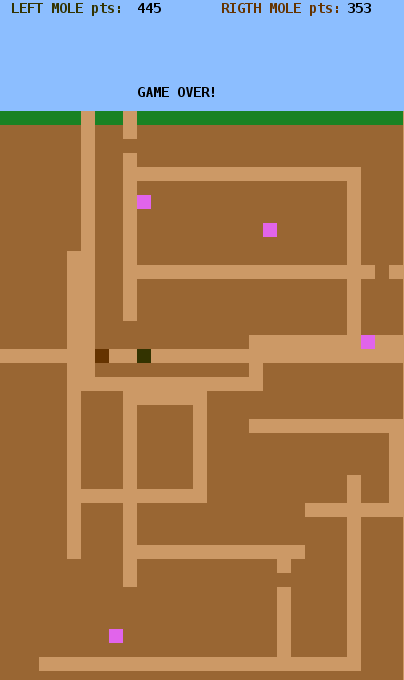
\includegraphics[width=1.0\textwidth]{../img/blockbattle.png}
  \caption{En duell om blockmaskar mellan två lundensiska blockmullvader fångade på bild under intensivt grävanade.}
  \label{lab:blockbattle:fig:game}
\end{figure}
\end{minipage}%
}%
\newlength{\currentparskip}%
\newlength{\currentparindent}%
{
\setlength{\currentparskip}{\parskip}% save the value
\setlength{\currentparindent}{\parindent}% save the value
\hfill%
\begin{minipage}{0.47\textwidth}
\setlength{\parskip}{\currentparskip}% restore the value
\setlength{\parindent}{\currentparindent}% restore the value
\noindent Under denna laboration ska du träna på att deklarera klasser och skapa flera instanser av samma klass. Du tränar även på att bygga ett större program från grunden.

Du ska utveckla ett spel för två spelare som sitter vid samma tangentbord, där den vänstra spelaren styr en blockmullvad med tangenterna A,S,D,W, och den högra spelaren styr en annan blockmullvad med piltangenterna.

I bilden till vänster ser du hur spelet kan se ut. Det finns en ljusbrun och en mörkbrun mullvad. Poängräkningen visas överst i himlen. Det finns fyra rosa blockmaskar (se uppgift \ref{lab:blockmole:task:blockworm} i laboration \code{blockmole}) som mullvadarna tävlar om att försöka fånga. När en blockmask teleporterar sig till en ny slumpmässig position lämnar den jord efter sig. När en mullvad gräver sig upp till gräsytan blir det hål i gräset.
Det ger poäng att gräva tunnlar och att fånga blockmaskar.

Du bestämmer själv hur poängsättningen ska ske och kriteriet för när spelet är slut etc.
\end{minipage}%
}



\subsection{Obligatoriska krav}

Följande funktionella krav ska uppfyllas av ditt program:
\begin{itemize}[nosep, label={$\square$},]
%\item Det ska finnas två blockmullvadar, en för vänster spelare och en för höger spelare, som styrs med ASDW resp. piltangerna.
\item Varje mullvad rör sig i sin aktuella riktning tills användaren ändrar riktning genom att trycka på ''sin'' motsvarande knapp, t.ex. W eller pil-upp.
\item Då en mullvad går i mörkbrun jord ska ljusbruna tunnlar grävas.
\item Då en blockmullvad når fönstrets kant eller himlen ska dess riktning reverseras.
\item Det ska ge poäng att gräva tunnlar.
\item Varje spelares poäng ska visas under spelets gång.
\item Ett spel ska avslutas och \emph{Game over} visas när något valfritt kriterium uppfyllts.
%\item Vid \emph{Game over} ska man kunna välja att avsluta programmet eller spela igen.
\end{itemize}

\noindent Din kod ska utformas enligt dessa design-krav:
\begin{itemize}[nosep, label={$\square$}]
\item Ett \code{Game} skapas i huvudprogrammet med metoden \code{start} som kör igång spelet.
\item Konstanter ska namnges och placeras i lämpligt kompanjonsobjekt.
\item Varje klass med ev. tillhörande kompanjonsobjekt ska finnas i en egen kodfil och tillhöra paketet \code{blockbattle}.
\item Du ska utgå från klasserna som du implementerat i uppgift \ref{exe:classes:labprep} i övning \texttt{\ExeWeekFIVE}.
\item Klassen \code{BlockWindow} omvandlar till interna fönsterkoordinater. Övriga klasser ska använda block-koordinater.
\end{itemize}


\subsection{Valbara krav -- välj minst ett}

Du ska implementera minst ett (gärna flera) av dessa krav:
\begin{itemize}[nosep, label={$\square$}]
\item Det ska finnas lagom många blockmaskar (se labb \code{blockmole} uppg. \ref{lab:blockmole:task:blockworm},  sid. \pageref{lab:blockmole:task:blockworm}).
\item Blockmullvadarna ska även ha ett attribut som representerar hälsan, t.ex. ett numeriskt värde mellan 0 och 100. Hälsan ska försvagas något när man gräver tunnlar. Hälsan ska synas i spelfönstret, t.ex. som en sekvens med röda block i himlen som indikerar andelen av maxhälsan för resp. spelare.
\item Att springa på gräset ska påverka poäng och/eller hälsa.
\item Att fånga blockmask ska påverka poäng och/eller hälsa.
\item Det ska finnas gula blockdiamanter som ger många poäng om man tar dem först.
\item Det ska vid spelstart gå att välja namn på respektive blockmullvad och namnet ska synas i spelet vid poängutskriften.
\item Det ska gå fortare att gå i gångar jämfört med att gräva i jord.
\item Om en blockmullvad fångar en blockmask ska dess grävhastighet öka.
\item Om en blockmullvad krockar med en annan blockmullvad ska något hända, t.ex. att dess riktning reverseras.
\item Visa \emph{highscore} vid \emph{Game Over}.  Highscore sparas med \code{introprog.IO} i en fil som skapas om den inte finns annars läses in vid uppstart om den finns och uppdateras vid behov. Spara hela highscore-listan eller bara högsta poäng hittills.
\end{itemize}

\subsection{Förebredelser inför redovisningen}
\Checkpoint\noindent Innan du redovisar din implementation ska du muntligt kunna redogöra för följande:
\begin{itemize}[nosep, label={$\square$}]
  \item Studera någon annans spel och ge din kamrat minst ett tips om hur kodens läsbarhet kan förbättras. Skriv ner dina tips och beskriv dem vid redovisningen.
  \item Beskriv vilka åtgärder du gjort för att din kod ska vara lätt att läsa och förstå.
  \item Beskriv hur du stegvis utvecklat ditt program från enklare till mer avancerad funktionalitet, samt vilka buggar du upptäckt och fixat.
  \item Beskriv vilket eller vilka valfria krav som din implementation uppfyller.
  \item Beskriv hur du hade behövt ändra i klassen \code{Mole} för att det ska gå att skriva\\\code{new Mole().move().move().reverseDir().move()}
\end{itemize}

\subsection{Tips och förslag}

\begin{enumerate}[leftmargin=*]
  \item \textbf{Många små steg.} Kör kompilering under ändringsbevakning med \code{--watch} i ett eget terminalfönster, så att du vid varje ändring kan rätta ev. kompileringsfel. Kör och testa ditt program ett annat terminalfönster.

  \item \textbf{Inför bra namn}. Din kod blir lättare att läsa och ändra i om du hittar på bra namn på medlemmar och lägger dem på lämpligt ställe. T.ex. kan du samla globala spel-konstanter i kompanjonsobjektet till klassen \code{Game}. Du kan bygga vidare på nedan kod och lägga till medlemmar allteftersom du upptäcker att de behövs. Nedan finns exempelvis en funktion som ger bakgrundsfärgen för en viss y-koordinat, vilken är användbar när du ska återställa bakgrunden efter att en mullvad har flyttat sig.
\scalainputlisting[basicstyle=\ttfamily\fontsize{10}{12}\selectfont]{../workspace/w06_blockbattle/Game.scala}
% \begin{CodeSmall}
% object Game {
%   val windowSize = (30, 50)
%   val windowTitle = "EPIC BLOCK BATTLE"
%   val blockSize = 14
%   val skyRange    = 0 to 7
%   val grassRange  = 8 to 8
%   object Color { ??? }
%   def backgroundColorAtDepth(y: Int): java.awt.Color = ???
% }
%
% class Game(
%   val leftPlayerName: String  = "LEFT",
%   val rightPlayerName: String = "RIGHT"
% ) {
%  import Game.* // direkt tillgång till namn på medlemmar i kompanjon
%
%  val window    = new BlockWindow(windowSize, windowTitle, blockSize)
%  val leftMole  = ???
%  val rightMole = ???
%
%  def drawWorld(): Unit = ???
%
%  def eraseBlocks(x1: Int, y1: Int, x2: Int, y2: Int): Unit = ???
%
%  def update(mole: Mole): Unit = ???  // update, draw new, erase old
%
%  def gameLoop(): Unit = ???
%
%  def start(): Unit = {
%    println("Start digging!")
%    println(s"$leftPlayerName ${leftMole.keyControl}")
%    println(s"$rightPlayerName ${rightMole.keyControl}")
%    drawWorld()
%    gameLoop()
%  }
% }
% \end{CodeSmall}

 \item \textbf{Dela upp din kod i funktioner.} Din kod blir lättare att läsa och ändra i om du delar upp den i många små funktioner med bra namn. I \code{Game}-klassen ovan finns exempel på några användbara funktioner. Allteftersom du utvidgar ditt program kan du lägga till fler funktioner som t.ex. heter \code{showPoints}, \code{gameOver}, etc.

\item \textbf{Tänk igenom den övergripande strukturen.} Programmet du ska skriva i denna laboration är större än det du gjort tidigare. Det är därför viktigt att tänka igenom strukturen på ditt program, vilka klasser som har hand om vad och hur de samarbetar. Diskutera gärna med handledare om du är osäker på hur de koddelar du utvecklat i föregående veckas övning \ref{exe:classes:labprep}, klasserna \code{Pos}, \code{KeyControl}, \code{Mole} och \code{BlockWindow}, är tänkt at samverka. Var noga med att testa så de olika klasserna och deras metoder fungerar var för sig.     

\item \textbf{Utformning av \texttt{gameLoop()}}. I ett spel behövs en s.k. spel-loop \Eng{game loop} som upprepar den kod som ska köras vid varje ny skärmbild, ofta kallad \emph{frame}. I varje runda i spel-loopen sker uppdatering av data och ritning i spelfönstret, samt en lämplig fördröjning. En skiss på en typisk spel-loop visas nedan:
\begin{CodeSmall}
  var quit = false
  val delayMillis = 80

  def gameLoop(): Unit = 
    while !quit do
      val t0 = System.currentTimeMillis
      handleEvents()    // ändrar riktning vid tangenttryck etc.
      update(leftMole)  // flyttar, ritar, suddar, etc.
      update(rightMole)

      val elapsedMillis = (System.currentTimeMillis - t0).toInt
      Thread.sleep((delayMillis - elapsedMillis) max 0)
    end while
  end gameLoop
\end{CodeSmall}

\item \textbf{Hantering av händelser.} Ett \code{BlockWindow}, som du implementerade i uppgift \ref{exe:classes:labprep} i övning \texttt{\ExeWeekFIVE}, kan via anrop av \code{nextEvent} ge   \code{KeyPressed(key)} vid knapptryck och \code{WindowClosed} vid fönsterstängning. Om ingen händelse finns att behandla returneras \code{Undefined}. Använd en loop som betar av alla händelser tills \code{Undefined} påträffas, enligt nedan:

\begin{CodeSmall}
  def handleEvents(): Unit = 
    var e = window.nextEvent()
    while e != BlockWindow.Event.Undefined do
      e match 
        case BlockWindow.Event.KeyPressed(key) =>
          ???  // ändra riktning på resp. mullvad

        case BlockWindow.Event.WindowClosed =>
          ???  // avsluta spel-loopen
      
      e = window.nextEvent()
    end while
  end handleEvent
\end{CodeSmall}

\item \textbf{Flimmerfri grafik.} För att minska mängden flimmer \Eng{flicker} är det bäst att i varje iteration i spel-loopen (1) bara rita om det som ändrats för att minimera tiden som spenderas på att rita, och (2) vid ändringar rita nya delar före att gamla delar raderas. För att slippa mullvadsflimmer kan du ''\emph{rita först -- sudda sen}'' enligt nedan.\footnote{Inom spelutveckling använder man oftast istället så kallad \emph{double buffering} (eller till och med \emph{triple buffering}) för att få helt flimmerfri grafik. Det ligger dock bortom kursen och stöds inte av \code{PixelWindow}.}

% \begin{CodeSmall}
% val oldMolePos = mole.pos                  // save
% mole.move()                                // update
% window.setBlock(mole.pos, mole.color)      // draw new
% window.setBlock(oldMolePos, Color.tunnel)  // erase old
% \end{CodeSmall}

\begin{CodeSmall}
window.setBlock(mole.nextPos, mole.color) // draw new
window.setBlock(mole.pos, Color.tunnel)   // erase old
mole.move()                               // update
\end{CodeSmall}

\end{enumerate}


%!TEX encoding = UTF-8 Unicode

%!TEX root = ../compendium1.tex

\chapter{Arv, Gränssnitt}
\begin{itemize}[nosep]
\item klasser
\item arv
\item polymorfism
\item likhet
\item equals
\item accessregler
\item private
\item public
\item protected
\item private[this]
\item trait
\item inmixning
\item Any
\item AnyVal
\item AnyRef
\item Nothing\end{itemize}
\clearpage\section{Teori}
%!TEX encoding = UTF-8 Unicode
%!TEX root = ../lect-w07.tex

\Subsection{Vad är en sekvens?}

\ifkompendium\else
{
  \setbeamercolor{background canvas}{bg=black}
  \frame[plain]{\centering\Huge\textbf{\color{pink}{ORDNINGEN}\\SPELAR\\ROLL}}
}
\fi


\begin{Slide}{Vad är en sekvens?}  
\begin{itemize}
\item En sekvens är en \Emph{följd av element} som
  \begin{itemize}
  \item har \Alert{ordningsnummer} (t.ex. numrerade från noll)
  \item är av en viss \Alert{typ} (t.ex. heltal).
  \end{itemize}
  \pause
\item En sekvens kan innehålla flera element som är lika.
\item En sekvens kan vara \Alert{tom} och har då längden noll.
\item Exempel på en icke-tom sekvens med dubbletter:
\begin{REPLnonum}
scala> val xs = Vector(42, 0, 42, -9, 0, 5)
xs: scala.collection.immutable.Vector[Int] =
  Vector(42, 0, 42, -9, 0, 5)
\end{REPLnonum}
\pause
\item \Emph{Indexering} ger ett element via dess ordningsnummer:
\begin{REPLnonum}
scala> xs(2)
res0: Int = 42

scala> xs.apply(2)
res1: Int = 42
\end{REPLnonum}
\end{itemize}
\end{Slide}

\begin{Slide}{Exempel: En sträng är en sekvens av tecken}
\begin{REPLnonum}
scala> "haj po daj"
\end{REPLnonum}
Längd? 
Vad ligger på första platsen?
Elementtyp?
Dubbletter?
\pause
\begin{REPLnonum}
scala> "haj po daj".length
res1: Int = 10

scala> "haj po daj".apply(0)
res2: Char = h

scala> "haj po daj"(0)
res3: Char = h

scala> "haj po daj".distinct
res4: String = haj pod
\end{REPLnonum}

\end{Slide}


\begin{Slide}{Iterera över element i en sekvens}
\begin{itemize}
\item Att \Emph{iterera} \Eng{iterate}, ä.k. traversera \Eng{traverse}, innebär att \Alert{gå igenom} och behandla element i en samling. 
\item Exempel på iterering med \code{foreach}, \code{map}, \code{for}:
\begin{REPLnonum}
scala> val xs = Vector(1,2,3)
val xs: Vector[Int] = Vector(1, 2, 3)

scala> xs.foreach(x => println(x + 1)) 
2
3
4

scala> xs.map(_ + 1)
val res0: Vector[Int] = Vector(2, 3, 4)

scala> for x <- xs yield x - 1
val res1: Vector[Int] = Vector(0, 1, 2)

\end{REPLnonum}
\end{itemize}
\end{Slide}

\begin{Slide}{Lägg till i början och i slutet av en sekvens}
  \begin{itemize}
  \item Med metoderna \code{+:} och \code{:+} kan du skapa en ny sekvens med nya element tillagda i början resp. i slutet.
  \item Minnesregel: ''\Alert{Colon on the collection side}''
  \begin{REPLnonum}
  scala> val xs = Vector(1,2,3)
  scala> 42 +: xs         // ger ny Vector(42, 1, 2, 3)
  scala> xs :+ 42         // ger ny Vector(1, 2, 3, 42)
  \end{REPLnonum}
  \pause
  \item Semantik: operatornotation med operatorer som \Emph{slutar med kolon} är \Alert{högerassociativa}
  \item Anropet \code{42 +: xs} skrivs av kompilatorn om till \code{xs.+:(42)}
  \begin{REPL}
  scala> xs.+:(42)
  res4: scala.collection.immutable.Vector[Int] = Vector(42, 1, 2, 3)
  \end{REPL}
  \pause
  \item Konkatenering (sammanfogning) av sekvenser: \code{xs ++ ys}
  
  \end{itemize}
\end{Slide}


\begin{Slide}{Egenskaper hos några sekvenssamlingar i Scala}
\vspace{-0.5em}
\begin{itemize}\SlideFontSmall

\item \code{Vector}
  \begin{itemize}\SlideFontSmall
  \item \Emph{Oföränderlig}. Snabb på att skapa kopior med små förändringar.
  \item Allsidig prestanda: \Emph{bra till det mesta}.
  \end{itemize}

\item \code{List}
  \begin{itemize}\SlideFontSmall
  \item \Emph{Oföränderlig}. Snabb på att skapa kopior med små förändringar.
  \item Snabb indexering \& uppdatering \Emph{i början}.
  \item Smidig \& snabb vid \Emph{rekursiva} algoritmer.
  \item Långsam vid upprepad \Alert{indexering} på godtyckliga ställen.
  \end{itemize}

\item \code{ArrayBuffer}
  \begin{itemize}\SlideFontSmall
  \item \Alert{Föränderlig}: \Emph{snabb indexering \& uppdatering}.
  \item Kan \Emph{ändra storlek} efter allokering. Snabb att indexera överallt.
  \end{itemize}

\item \code{ListBuffer}
  \begin{itemize}\SlideFontSmall
  \item \Alert{Föränderlig}: snabb indexering \& uppdatering \Emph{i början}.
  \item Snabb om du bygger upp sekvens genom många tillägg i början.
  \end{itemize}

\item \code{Array} (använd fr.o.m. Scala 2.13 hellre \code{ArraySeq})
  \begin{itemize}\SlideFontSmall
  \item \Alert{Föränderlig}: \Emph{snabb indexering \& uppdatering}.
  \item Kan \Alert{ej ändra storlek}; storlek ges vid allokering.
  \item Har särställning i JVM: ger snabb allokering och access.
  \end{itemize}

\end{itemize}
\end{Slide}

\begin{Slide}{I stället för Array: \texttt{ArraySeq} (Scala >2.13)}
Nytt i Scala 2.13:
\begin{itemize}
  \item \code{collection.mutable.ArraySeq} fungerar lika bra som, eller bättre än \code{Array}
  \item \url{https://stackoverflow.com/questions/5028551/array-vs-arrayseq-comparison}
  \item \code{collection.immutable.ArraySeq} fungerar som en Array som inte kan ändras
  \item \code{WrappedArray} är från 2.13 \textit{deprecated} (på väg bort)
\end{itemize}
{\SlideFontTiny Fördjupning: Sammanfattning av prestanda för olika samlingar: \href{https://docs.scala-lang.org/overviews/collections-2.13/performance-characteristics.html}{docs.scala-lang.org/overviews/collections-2.13/performance-characteristics.html}
}
\end{Slide}

\begin{Slide}{Vilken sekvenssamling ska jag välja?}\SlideFontSmall
\vspace{-0.5em}
\begin{itemize}
\item Välj \code{Vector} om ...
  \begin{itemize}\SlideFontTiny
  \item[a)] du vill ha oföränderlighet: \code{val xs = Vector[Int](1,2,3)}
  \item[b)] du behöver föränderlighet (notera \code{var}):\\ \code{var xs = Vector.empty[Int]}
  \item[c)] du ännu inte vet vilken sekvenssamling som är bäst; du kan alltid ändra efter att du mätt prestanda och kollat flaskhalsar vid upprepade körningar.
  \end{itemize}

\item Välj \code{List} om ...
  \begin{itemize}\SlideFontTiny
  \item[] du har en \Alert{rekursiv} sekvensalgoritm och/eller \Alert{mestadels jobbar i början}.
  \end{itemize}

\item Välj \code{ArrayBuffer} om ...
  \begin{itemize}\SlideFontTiny
  \item[] det behövs av prestandaskäl och du \Alert{inte} vet storlek vid allokering:\\
  \code{val xs = scala.collection.mutable.ArrayBuffer.empty[Int]}
  \end{itemize}

\item Välj \code{ListBuffer} om ...
  \begin{itemize}\SlideFontTiny
  \item[] det behövs av prestandaskäl och du bara behöver lägga till i början:\\ \code{val xs = scala.collection.mutable.ListBuffer.empty[Int]}
  \end{itemize}

\item Välj \code{Array} eller \code{ArraySeq} om ...
  \begin{itemize}\SlideFontTiny
  \item[] det verkligen behövs av prestandaskäl och du \Alert{vet} storlek vid allokering:\\
  \code{val xs = Array.fill(initSize)(initValue)}
  \end{itemize}

\end{itemize}
\end{Slide}

\begin{Slide}{Några konstigheter med Array}
\begin{itemize}
\item Referenslikhet istf innehållslikhet: 
\begin{REPLnonum}
scala> Vector(1,2,3) == Vector(1,2,3)
val res0: Boolean = true

scala> Array(1,2,3) == Array(1,2,3)
val res1: Boolean = false  // aaargh!!
\end{REPLnonum}
\item Special-syntax för att skapa utan explicit initialisering: \\
{\SlideFontSmall\code{val xs = new Array[String](1000)  // 1000 null-referenser}}
\item Fungerar inte lika bra med generiska typer:
\begin{REPLnonum}
scala> def box[T](x: T) = Vector[T](x)  //funkar fint

scala> def abox[T](x: T) = Array[T](x)
  error: No ClassTag available for T
\end{REPLnonum}
\end{itemize}
\end{Slide}

\begin{Slide}{Oföränderlig eller förändringsbar?}
\begin{itemize}
\item \Emph{Oföränderlig}:  Kan ej ändra elementreferenserna, men effektiv på att skapa kopia som är (delvis) förändrad \Emph{Vector} eller \Emph{List}

\item \Alert{Förändringsbar}: kan ändra elementreferenserna
  \begin{itemize}
  \item Kan \Alert{ej ändra storlek} efter allokering: \\ \Emph{Array} eller \Emph{ArraySeq}: indexera och uppdatera varsomhelst
  \item Kan även ändra storlek efter allokering:
  \\\Alert{ArrayBuffer} eller \Alert{ListBuffer}
  %\\ Java: \Alert{ArrayList} eller \Alert{LinkedList}
  \end{itemize}
\item \Emph{Ofta funkar oföränderlig sekvenssamling utmärkt}, men om man \Alert{efter prestandamätning} upptäcker en flaskhals kan man ändra från \Emph{Vector} till t.ex. \Emph{ArrayBuffer}.
\end{itemize}
\end{Slide}



\Subsection{Vad är en sekvensalgoritm?}



\begin{Slide}{Vad är en sekvensalgoritm?}\SlideFontTiny
\begin{itemize}
\item En algoritm är en stegvis beskrivning av lösningen på ett problem.
\item En \textbf{sekvensalgoritm} är en algoritm där \Emph{element i sekvens} utgör en viktig del av \Alert{problembeskrivningen} och/eller \Alert{lösningen}.
\item Exempelproblem: sortera en sekvens av personer efter deras ålder.
\pause
\item \Alert{Sju} ofta återkommande programmeringsproblem som löses med en sekvensalgoritm:
\begin{itemize}\SlideFontTiny
\item \Emph{Kopiering} av alla element i en sekvens till en \Alert{ny} sekvens
\item \Emph{Uppdatering} av sekvensen: ta bort, lägga till, ändra \Emph{enskilda} element
\item \Emph{Transformering}: applicera en \Alert{funktion} på \Emph{alla} element   
\item \Emph{Filtrering}: urval av vissa element som uppfyller ett \Alert{villkor}
\item \Emph{Sökning} efter ett element som uppfyller ett \Alert{sökkriterium}
\item \Emph{Sortering} enligt någon \Alert{ordning}
\item \Emph{Registrering} av \Alert{frekvens} av element med vissa \Alert{egenskaper}
\end{itemize}
\end{itemize}
\href{https://youtu.be/0ArlUSVDQIw?t=27s}{\textbf{KUT FSSR}} 
\end{Slide}

\ifkompendium\else
{
  \setbeamercolor{background canvas}{bg=black}
  \frame[plain]{\centering\Huge\textbf{\color{pink}{ORDNINGEN\\SPELAR\\ROLL}\\\color{red}{KUT FSSR}}}
}
\fi



\Subsection{Använda färdiga sekvenssamlingsmetoder}


\begin{Slide}{Använda färdiga sekvenssamlingsmetoder}
\begin{itemize}\SlideFontSmall
\item Standardbiblioteket i Scala innehåller flera olika samlingar som har sekvensegenskaper, t.ex. \code{Vector} och \code{ArrayBuffer}, som erbjuder olika möjligheter och har olika prestanda beroende på vad man vill göra.
\item Scala 3 använder samma samlingsbibliotek som i Scala 2.13, se intro:  \url{https://docs.scala-lang.org/overviews/collections-2.13/introduction.html} 

\item Ofta kan man implementera sekvensalgoritmer genom anrop av en eller flera \Alert{färdiga} metoder.

\item Dessa färdiga metoder är \Emph{optimerade och vältestade} och är att föredra om möjligt.

\item Studera Scalas api-dokumentation och kursens quickref för att se vad man kan göra med färdiga metoder.

\item Det är \Emph{lärorikt} att ''\Alert{uppfinna hjulet}'' och implementera några sekvensalgoritmer \Emph{själv} för bättre förståelse, även om de redan finns färdiga i Scalas samlingsbibliotek.

\end{itemize}
\end{Slide}



\begin{Slide}{Några användbara samlingsmetoder vid implementation av sekvensalgoritmer}
\SlideFontTiny
\begin{tabular}{@{}l l}
\code|xs.map(f)|           & transformering, motsv. \code|for x <- xs yield f(x)| \\
\code|xs.map(x => x)|    & kopiering, motsv. \code|for x <- xs yield x| \\
\code|xs.filter(p)|        & filtrering, ta med x om p(x)\\
\code|xs.filterNot(p)|     & filtrering, ta med x om !p(x)\\
\code|xs.distinct|        & filtrering, ta bort dubbletter \\
\code|xs.take(n)|          & ny sekvens med de första n elements, resten skippade\\ 
\code|xs.drop(n)|          & ny sekvens där de första n elements är skippade\\ 
\code|xs.takeWhile(p)|     & filtrera, ta med i början så länge p(x)  \\
\code|xs.dropWhile(p)|     & filtrera, skippa i början så länge p(x)  \\
\code|xs.find(p)|       & sök framifrån efter första element x där p(x) är sant\\
\code|xs.indexOf(x)|       & sök framifrån efter index för element som är samma som x \\
\code|xs.lastIndexOf(x)|   & sök bakifrån efter index för element som är samma som x \\
\code|xs.sorted|          & sortera med inbyggd (implicit given) ordning \\
\code|xs.sorted.reverse| & sortera i omvänd ordning \\
\code|xs.sortBy(f)|        & sortera i ordning enligt f(x)\\
\code|xs.sortWith(lt)|     & sortera enligt ''less than''-funktionen \code|lt: (A, A) => Boolean|\\
\code|xs.count(p)|         & räkna antalet element där p(x) är sant
\end{tabular}

\vspace{0.5em}%
\Emph{Lär dig fler smidiga metoder i} \Alert{quickref}
\end{Slide}

\begin{Slide}{Uppdaterad sekvens med kraftfulla metoden \texttt{patch}}
  Metoden \code{patch} kan användas så: \code{xs.patch(fromPos, ys, nbrReplaced)} \\för att skapa en \Alert{ny} sekvens där \Emph{ett} eller \Emph{flera} element i xs är...  
  \begin{itemize}
    \item utbytta \Eng{replaced}
    \item borttagna \Eng{removed}
    \item tillagda \Eng{inserted}
  \end{itemize}
  .. med nya element ur \code{ys} 
\begin{REPL}
scala> val xs = Vector(1,2,3)

scala> xs.patch(2, Vector(-1), 1)     // replaced one elem
res0: scala.collection.immutable.Vector[Int] = Vector(1, 2, -1)

scala> xs.patch(1, Vector(42), 0)     // inserted one elem
res11: scala.collection.immutable.Vector[Int] = Vector(1, 42, 2, 3)

scala> xs.patch(0, Vector(), 2)       // removed two elems
res2: scala.collection.immutable.Vector[Int] = Vector(3)
 
\end{REPL}
\end{Slide}

\begin{Slide}{Använda for-uttryck för filtrering med hjälp av gard}
I ett for-uttryck kan man ha en \Emph{gard} \Eng{guard} i form av ett booleskt uttryck efter nyckelordet \code{if}. Då kommer uttrycket efter \code{yield} bara göras om gard-uttrycket är sant.

\vspace{1em}

Syntaxen är så här: (parenteser behövs ej runt gard-uttrycket)
\begin{Code}[basicstyle=\ttfamily\SlideFontSize{12}{14}]
for x <- xs if uttryck1 yield uttryck2
\end{Code}
\pause
Exempel:
\begin{REPLnonum}
scala> val udda = for x <- 1 to 6 if x % 2 == 1 yield x
\end{REPLnonum}
\pause
\code{udda} blir \code{Vector(1, 3, 5)}
\end{Slide}


\begin{Slide}{Använda samlingsmetoden \texttt{filter} för filtrering}
Alla samlingar i \code{scala.collection} har metoden \code{filter}. Den har ett predikat som parameter \code{p: T => Boolean} och ger en ny samling med de element för vilka predikatet är sant.
\begin{Code}[basicstyle=\ttfamily\SlideFontSize{12}{14}]
xs.filter(p)
\end{Code}
\pause
Exempel: Antag att \code{xs} är \code{(1 to 6).toVector}
\begin{REPLnonum}
xs.filter(_ % 2 == 1)
\end{REPLnonum}
\pause
uttryckets resultat blir \code{Vector(1, 3, 5)}, vilket motsvarar:
\begin{Code}[basicstyle=\ttfamily\SlideFontSize{10}{13}]
for x <- xs if x % 2 == 1 yield x
\end{Code}
\pause
I själva verket skriver Scala-kompilatorn om for-uttryck med gard till anrop av metoden \code{filter} före kodgenerering sker.
\end{Slide}


\begin{Slide}{Vanliga sekvensproblem som funktionshuvuden}
Indata och utdata för några vanliga sekvensproblem:
\begin{Code}
def copy(xs: Vector[Int]): Vector[Int] = ???

def filter(xs: Vector[Int], p: Int => Boolean): Vector[Int] = ???

def findIndices(xs: Vector[Int], p: Int => Boolean): Vector[Int] = ???

def sort(xs: Vector[Int]): Vector[Int] = ???

def freq(xs: Vector[Int]): Vector[(Int, Int)] = ???  // (heltal, frekvens)
\end{Code}
Övning: Hur implementera dessa med \code{for}-uttryck och/eller färdiga samlingsmetoder?\\
\Emph{Tips:} För \code{sort}\&\code{freq} se \code{sorted}, \code{distinct}, \code{count} i \href{http://cs.lth.se/pgk/quickref/}{quickref}
\end{Slide}


\begin{Slide}{Implementation av sekvensproblem med \texttt{for}-uttryck och/eller färdiga samlingsmetoder}
\begin{Code}
def copy(xs: Vector[Int]): Vector[Int] = for x <- xs yield x

def filter(xs: Vector[Int], p: Int => Boolean): Vector[Int] =
  for x <- xs if p(x) yield x

def findIndices(xs: Vector[Int], p: Int => Boolean): Vector[Int] =
  (for i <- xs.indices if p(xs(i)) yield i).toVector

def sort(xs: Vector[Int]): Vector[Int] = xs.sorted // mer om sortering sen

def freq(xs: Vector[Int]): Vector[(Int, Int)] = // mer om registrering snart
  for x <- xs.distinct yield x -> xs.count(_ == x)
\end{Code}
Övning: Hur implementera dessa med \code{map} och \code{filter} och/eller andra färdiga samlingsmetoder?
\end{Slide}

\begin{Slide}{Implementation av sekvensproblem med \texttt{map}, \texttt{filter}}
\begin{Code}
def copy(xs: Vector[Int]): Vector[Int] = xs.map(x => x)

def filter(xs: Vector[Int], p: Int => Boolean): Vector[Int] = xs.filter(p)

def findIndices(xs: Vector[Int], p: Int => Boolean): Vector[Int] =
  xs.indices.filter(i => p(xs(i))).toVector

def sort(xs: Vector[Int]): Vector[Int] = xs.sorted // mer om sortering sen

def freq(xs: Vector[Int]): Vector[(Int, Int)] = // mer om registrering snart
  xs.distinct.map(x => x -> xs.count(_ == x))
\end{Code}
%Fördjupningsövning: Hur göra dessa metoder generiska för alla sekvenssamlingar av typen \code{Seq[T]}?
\end{Slide}


\begin{Slide}{Hierarki av samlingstyper i \texttt{scala.collection} v2.13}

  \begin{multicols}{2}
  \begin{tikzpicture}[sibling distance=5.0em,->,>=stealth', inner sep=3pt, %scale=0.5,
    every node/.style = {shape=rectangle, draw, align=center,font=\small\ttfamily},
    class/.style = {fill=blue!20},
    trait/.style = {rounded corners, fill=red!20}]
    \node[trait] {Iterable}
        child { node[trait] {Seq} }
        child { node[trait] {Set} }
        child { node[trait] {Map} }
      ;
  \end{tikzpicture}
  
  \columnbreak
  
  {\SlideFontTiny
  
  \code{Iterable} har metoder som är implementerade med hjälp av: \\
  \code{def foreach[U](f: Elem => U): Unit}\\
  \code{def iterator: Iterator[A] }
  
}

\begin{itemize}\SlideFontTiny
  \item[] \code{Seq}: ordnade i sekvens
  \item[] \code{Set}: unika element
  \item[] \code{Map}: par av (nyckel, värde)
  \end{itemize}
  
  
  \end{multicols}
  
  {\SlideFontSmall Samlingen \Emph{\texttt{Vector}} är en \code{Seq} som är en \code{Iterable}. \\ \vspace{0.5em}\pause
  De konkreta samlingarna är uppdelade i dessa paket:\\
  \code{scala.collection.immutable} \hfill där flera är \Emph{automatiskt} importerade\\
  \code{scala.collection.mutable}  \hfill som \Alert{måste importeras} explicit\\\pause
  (undantag: primitiva \code{scala.Array})
  }
\end{Slide}
  


\begin{Slide}{Lämna det öppet: använd \texttt{Seq}}\SlideFontSmall
Typen \Emph{\code{collection.immutable.Seq}} är supertyp till alla sekvenssamlingar i \code{collection.immutable}.
\pause Exempel: kopiering av sekvens:
\begin{itemize}
\item Kopiering av \Alert{specifik} heltalssekvens:
\begin{Code}
def copyIntVector(xs: Vector[Int]): Vector[Int] = for x <- xs yield x
\end{Code}

\item Kopiering som fungerar för alla oföränderliga heltalssekvenser:
\begin{Code}
def copyIntSeq(xs: Seq[Int]): Seq[Int] = for x <- xs yield x
\end{Code}
\end{itemize}
\pause
\begin{REPL}
scala> val xs = Vector(1,2,3)
xs: Vector[Int] = Vector(1, 2, 3)

scala> val ys = copyIntVector(xs)
ys: Vector[Int] = Vector(1, 2, 3)

scala> val zs = copyIntSeq(xs)
val zs: Seq[Int] = Vector(1, 2, 3)
\end{REPL}
%  Någon lämplig specifik samling som är subtyp till \code{Seq[T]} väljs automatiskt. \\
% (Mer om typparametrar och supertyper/subtyper senare i kursen.)
% \begin{Code}[basicstyle=\ttfamily]
% def varannanBaklänges[T](xs: Seq[T]): Seq[T] =
%   for i <- xs.indices.reverse by -2 yield xs(i)
% \end{Code}
% Fungerar med alla sekvenssamlingar:
% \begin{REPLnonum}
% scala> varannanBaklänges(Vector(1,2,3,4,5))
% res0: Seq[Int] = Vector(5, 3, 1)
%
% scala> varannanBaklänges(List(1,2,3,4,5))
% res1: Seq[Int] = List(5, 3, 1)
%
% scala> varannanBaklänges(collection.mutable.ListBuffer(1,2))
% res2: Seq[Int] = Vector(2)
% \end{REPLnonum}
% Scalas standardbibliotek returnerar ofta lämpligaste specifika sekvenssamlingen som är subtyp till \texttt{Seq[T]}.
\end{Slide}
  
\begin{Slide}{Implementation med generiska funktioner}\SlideFontSmall
Genom att generalisera funktionshuvudena blir våra lösningar användbara för \Alert{alla} sekvenser av typen \code{Seq[T]}, där den obundna \Emph{typparametern} \code{T} vid anrop kan bindas till godtycklig typ. (Mer om typparametrar senare.)
\begin{Code}
def copy[T](xs: Seq[T]): Seq[T] = xs.map(x => x)

def filter[T](xs: Seq[T], p: T => Boolean): Seq[T] = xs.filter(p)

def findIndices[T](xs: Seq[T], p: T => Boolean): Seq[Int] =
  xs.indices.filter(i => p(xs(i))).toVector

def sort[T: Ordering](xs: Seq[T]): Seq[T] = xs.sorted // mer om Ordering sen

def freq[T](xs: Seq[T]): Seq[(T, Int)] =
  xs.distinct.map((_, xs.count(_ == x)))
\end{Code}
\pause
Standardbibliotekets metoder försöker ordna så att det blir samma konkreta typ in som ut, men ibland väljs annan lämplig konkret samling, t.ex. kan en \code{Array} bli en \code{ArrayBuffer}. 
\end{Slide}

\begin{Slide}{Använda Java-samlingar i Scala med \texttt{CollectionConverters}}\SlideFontSmall
Med hjälp av \code{import scala.jdk.CollectionConverters.*} \\
får man smidig \Emph{interoperabilitet} med Java och dess standardbibliotek, \\
speciellt metoderna \Alert{\code{asJava}} och \Alert{\code{asScala}}:
\begin{REPL}
scala> import scala.jdk.CollectionConverters.*

scala> Vector(1,2,3).asJava
res0: java.util.List[Int] = [1, 2, 3]

scala> val xs = new java.util.ArrayList[String]()
xs: java.util.ArrayList[String] = []

scala> xs.add("hej")
res1: Boolean = true

scala> xs.asScala
res2: scala.collection.mutable.Buffer[String] = Buffer(hej)
\end{REPL}

\noindent Läs mer här: %
\ifkompendium\\\fi%
\scriptsize%
\url{https://docs.scala-lang.org/overviews/collections-2.13/conversions-between-java-and-scala-collections.html}

\end{Slide}


\begin{Slide}{Fördjupning: Skapa generisk Array}\SlideFontTiny
\begin{itemize}
\item I JVM bytekod går det tyvärr \Alert{inte} att skapa en primitiv generisk array.

\item Maskinkoden måste istället skapa en array av den mest generella referenstypen \code{Object} 
och sedan \Alert{typtesta och typkonvertera under körtid}.\\ Se t.ex. Java-implementationen av \code{ArrayList}:\\\href{http://developer.classpath.org/doc/java/util/ArrayList-source.html}{http://developer.classpath.org/doc/java/util/ArrayList-source.html} %på rad 119
\item[]
\item Men det \Emph{\emph{går}} att skapa en generisk array i Scala (men inte i Java). Då behövs en \code{reflect.ClassTag} som möjliggör typinformation vid körtid för arrayer. \\
\begin{REPLsmall}
scala> def fyll[T](n: Int, x: T): Array[T] = Array.fill(n)(x)
-- Error:
1 |def fyll[T](n: Int, x: T): Array[T] = Array.fill(n)(x)
  |                                                      ^
  |  No ClassTag available for T

scala> def fyll[T: reflect.ClassTag](n: Int, x: T): Array[T] = Array.fill(n)(x)

scala> fyll(42, "hej")
res2: Array[String] = Array(hej, hej, hej, hej, hej, hej, hej, hej, hej, hej, hej, hej, hej, hej, hej, hej, hej, hej, hej, hej, hej, hej, hej, hej, hej, hej, hej, hej, hej, hej, hej, hej, hej, hej, hej, hej, hej, hej, hej, hej, hej, hej)

\end{REPLsmall}
\item Kompilatorn skapar då maskinkod som automatiskt gör typkonverteringarna.

\end{itemize}
\end{Slide}

%!TEX encoding = UTF-8 Unicode
%!TEX root = ../lect-w07.tex

%%%

\Subsection{Repeterade parametrar}

\begin{Slide}{Repeterade parametrar blir sekvens}\SlideFontSmall
Med en asterisk efter parametertypen kan antalet argument variera:
\begin{Code}[basicstyle=\fontsize{10}{12}\selectfont\ttfamily]
def sumSizes(xs: String*): Int = xs.map(_.length).sum
\end{Code}
\begin{REPLnonum}
scala> sumSizes("Zaphod")
res0: Int = 6

scala> sumSizes("Zaphod","Beeblebrox")
res1: Int = 16

scala> sumSizes("Zaphod","Beeblebrox","Ford","Prefect")
res3: Int = 27

scala> sumSizes()
res4: Int = 0
\end{REPLnonum}
Repeterade parametrar \Eng{repeated parameters} blir en sekvens av typen \code{Seq} och som mer specifikt är en \code{ArraySeq}
\end{Slide}


\begin{Slide}{Sekvenssamling som argument till repeterade parametrar}
\begin{Code}[basicstyle=\fontsize{10}{12}\selectfont\ttfamily]
def sumSizes(xs: String*): Int = xs.map(_.size).sum

val veg = Vector("gurka","tomat")
\end{Code}
Om du \emph{redan har} en sekvenssamling så kan du applicera den på en funktion
som har repeterade parametrar med hjälp av en asterisk \code{*} \\
\vspace{1em}Den ska skrivas direkt \Alert{efter} den sekvenssamling, som du vill att kompilatorn ska tolka som en sekvens av argument, så här:
\begin{REPLnonum}
scala> sumSizes(veg*)
res5: Int = 10
\end{REPLnonum}

\end{Slide}

%!TEX encoding = UTF-8 Unicode
%!TEX root = ../lect-w07.tex

%%%

\Subsection{Registrering}

\begin{Slide}{Registrering}
\begin{itemize}
\item \Emph{Registrering} innefattar algoritmer för att räkna antalet förekomster av olika saker.

\item Exempel:
\\\vspace{0.5em}Utfallsfrekvens vid kast med en tärning 1000 gånger:

\vspace{1em}\begin{tabular}{r c l}
utfall & & antal \\ \hline
1 & $\rightarrow$ & 178 \\
2 & $\rightarrow$ & 187 \\
3 & $\rightarrow$ & 167 \\
4 & $\rightarrow$ & 148 \\
5 & $\rightarrow$ & 155 \\
6 & $\rightarrow$ & 165 \\
\end{tabular}
\end{itemize}
\end{Slide}

\begin{Slide}{Registrering av tärningskast i \code{Array}}
Vi låter plats 0 representera antalet ettor, plats 1 representerar antalet tvåor etc. \Alert{Övning}: implementera \code{???}
\begin{REPLnonum}
scala> def rollDice(): Int = ???  //dra slumptal 1-6

scala> val reg = ???  //skapa heltalsarray m 6 platser
reg: Array[Int] = Array(0, 0, 0, 0, 0, 0)

scala> for (i <- 1 to 1000) ???  //kasta tärning, registrera

scala> for (i <- 1 to 6) println(i +": " + reg(i - 1))
1: 178
2: 187
3: 167
4: 148
5: 155
6: 165
\end{REPLnonum}
\end{Slide}


\begin{Slide}{Registrering av tärningskast i \code{Array}}
Vi låter plats 0 representera antalet ettor, plats 1 representerar antalet tvåor etc. \Emph{Lösning}:
\begin{REPLnonum}
scala> def rollDice() = scala.util.Random.nextInt(6) + 1

scala> val reg = new Array[Int](6)
reg: Array[Int] = Array(0, 0, 0, 0, 0, 0)

scala> for (i <- 1 to 1000) reg(rollDice - 1) += 1

scala> for (i <- 1 to 6) println(i +": " + reg(i - 1))
1: 178
2: 187
3: 167
4: 148
5: 155
6: 165
\end{REPLnonum}
\end{Slide}

% \begin{Slide}{Registrering av tärningskast i \code{Map}, imperativ lösning}
% Vi registrerar antalet i en Map[Int, Int] där nyckeln är antalet tärningsögon och värdet är frekvensen.
% \begin{REPLnonum}
% scala> val rnd = new java.util.Random(42L)
% rnd: java.util.Random = java.util.Random@6d946eee
%
% scala> var reg = (1 to 6).map(i => i -> 0).toMap
% reg: scala.collection.immutable.Map[Int,Int] =
%   Map(5 -> 0, 1 -> 0, 6 -> 0, 2 -> 0, 3 -> 0, 4 -> 0)
%
% scala> for (i <- 1 to 1000) {
%          val t = rnd.nextInt(6) + 1
%          reg = reg + ((t, reg(t) + 1))
%        }
%
% scala> reg
% res0:scala.collection.immutable.Map[Int,Int]= Map(5 -> 155,
% 1 -> 178, 6 -> 165, 2 -> 187, 3 -> 167, 4 -> 148)
% \end{REPLnonum}
% \end{Slide}
%
% \begin{Slide}{Registrering av tärningskast i \code{collection.mutable.Map}, imperativ lösning}
% Om vi är bekymrade över prestanda:
% \begin{REPL}
% scala> val rnd = new java.util.Random(42L)
% rnd: java.util.Random = java.util.Random@6d946eee
%
% scala> val initPairs = (1 to 6).map(i => i -> 0)
% initPairs: scala.collection.immutable.IndexedSeq[(Int, Int)] =
% Vector((1,0), (2,0), (3,0), (4,0), (5,0), (6,0))
%
% scala> var reg = scala.collection.mutable.Map(initPairs: _*)
%
% scala> for (i <- 1 to 1000) {
%          val t = rnd.nextInt(6) + 1
%          reg(t) = reg(t) + 1
%        }
%
% scala> reg
% res0: scala.collection.mutable.Map[Int,Int] =
% Map(2 -> 187, 5 -> 155, 4 -> 148, 1 -> 178, 3 -> 167, 6 -> 165)
%
% \end{REPL}
% \end{Slide}
%
% \begin{Slide}{Registrering av tärningskast i \code{Map}, funktionell lösning}
% Oföränderlighet: Skapa nya samlingar utan att ändra något.
% \begin{REPLnonum}
% scala> val rnd = new java.util.Random(42L)
% rnd: java.util.Random = java.util.Random@6d946eee
%
% scala> val dice = (1 to 1000).map(i => rnd.nextInt(6) + 1)
%
% scala> dice.groupBy(i => i).mapValues(_.size)
% res0:scala.collection.immutable.Map[Int,Int]= Map(5 -> 155,
% 1 -> 178, 6 -> 165, 2 -> 187, 3 -> 167, 4 -> 148)
% \end{REPLnonum}
% Övn. för den nyfikne: mät prestanda för de olika lösningarna.
% \end{Slide}

% \ifkompendium\else
% \begin{SlideExtra}{Syresättning av hjärnan med registreringslek}\SlideFontTiny

% \vspace{-0.65em}\scalainputlisting[numbers=left,numberstyle=,basicstyle=\SlideFontSize{6}{8}\ttfamily\selectfont]{../compendium/examples/sequences/RegisterToggleWinner.scala}
% Övning: Vad gör koden?
% % \begin{Code}
% % object StandUpSleepyBrain {
% %   def randomChar: Char = (scala.util.Random.nextInt('Z' - 'A' + 1) + 'A').toChar
% %   val reg = new Array[Int]('Z' - 'A' + 1)
% %   def tab: Seq[(Char, Int)] = reg.indices.map(i => ((i + 'A').toChar, reg(i)))
% %   def winner = "\n ** Toggle Winner: **" + (reg.indexOf(reg.max)+'A').toChar
% %   def report = "Registreringsrapport:\n" + tab.mkString("\n") + winner
% %
% %   def toggle(n: Int = 10): Unit = {
% %     println(s"Toggla (sitt upp/sitt ner) om ditt förnamn börjar på: ")
% %     var ready = false
% %     while(!ready){
% %       val chars = Vector.fill(n)(randomChar).distinct.sorted
% %       println("\n" + chars.mkString(" "))
% %       chars.foreach(ch => reg(ch - 'A') += 1)
% %       ready = scala.io.StdIn.readLine("\n").length > 0
% %     }
% %     println(report)
% %   }
% % }
% % \end{Code}
% \vspace{-0.5em}Kör koden och lyssna på: \href{https://youtu.be/ZVrgj3A0_BY}{https://youtu.be/ZVrgj3A0\_BY}
% \end{SlideExtra}
% \fi
%!TEX encoding = UTF-8 Unicode
%!TEX root = ../lect-w07.tex

\Subsection{Skapa lösningar på sekvensproblem från grunden}

\begin{Slide}{Skapa lösningar på sekvensproblem från grunden}
  \begin{itemize}
    \item Normalt använder man färdiga samlingsmetoder
    \item Det finns ofta en färdig metod som gör det man vill
    \item Annars kan man ofta göra det man vill genom att kombinera flera färdiga samlingsmetoder
    \item[] \pause
    \item Vi ska nu i lärosyfte implementera några egna varianter av uppdatering från grunden.  
  \end{itemize}

{\SlideFontSmall  För problem av typen KUTFSSR ingår det i kursen att kunna 1) lösa dessa med färdiga samlingsmetoder, och 2) implementera egna lösningar med hjälp av sekvens, alternativ, repetition, abstraktion (\textbf{SARA}).
}
\end{Slide}

\begin{Slide}{Skapa ny sekvenssamling eller ändra på plats?}
Två olika principer vid sekvensalgoritmkonstruktion:
\begin{itemize}
\item Skapa \Emph{ny sekvens} utan att förändra insekvensen
\item Ändra \Emph{på plats} \Eng{in-place} i \Alert{förändringsbar} sekvens
\end{itemize}
\pause
\vspace{1em}
Välja mellan att skapa ny sekvens eller ändra på plats?
\begin{itemize}
\item Ofta är det \Emph{lättast att skapa ny samling} och kopiera över elementen efter eventuella förändringar medan man loopar.
\item Om man har mycket stora samlingar kan man behöva ändra på plats för att spara tid/minne.
\end{itemize}
\end{Slide}

\begin{Slide}{Algoritm: SEQ-COPY}
\Emph{Pseudokod} för algoritmen SEQ-COPY som kopierar en sekvens, här en Array med heltal:\\
\noindent\hrulefill
\begin{algorithm}[H]
 \SetKwInOut{Input}{Indata}\SetKwInOut{Output}{Resultat}
 \Input{Heltalsarray $xs$}
 \Output{En ny heltalsarray som är en kopia av $xs$. \\ \vspace{1em}}
 $result \leftarrow$ en ny array med plats för $xs.length$ element\\
 $i \leftarrow 0$  \\
 \While{$i < xs.length$}{
  $result(i) \leftarrow xs(i)$\\
  $i \leftarrow i + 1$\\
 }
 \Return $result$
\end{algorithm}
\noindent\hrulefill
\end{Slide}

\begin{Slide}{Implementation av SEQ-COPY med \texttt{while}}
\lstinputlisting[numbers=left]{../compendium/examples/workspace/w05-seqalg/src/seqCopy.scala}
\end{Slide}

% \begin{Slide}{Implementation av SEQ-COPY med \texttt{for}}
% \lstinputlisting[numbers=left]{../compendium/examples/workspace/w05-seqalg/src/seqCopyFor.scala}
% \end{Slide}
%
% \begin{Slide}{Implementation av SEQ-COPY med \texttt{for-yield}}
% \lstinputlisting[numbers=left]{../compendium/examples/workspace/w05-seqalg/src/seqCopyForYield.scala}
% \end{Slide}

%!TEX encoding = UTF-8 Unicode
%!TEX root = ../lect-w07.tex

%%%


\Subsection{Implementera insert, remove, append}


\begin{Slide}{Exempel: PolygonWindow}\SlideFontTiny
\setlength{\leftmargini}{0pt}
\begin{itemize}
\item En polygon kan representeras som en punktsekvens, där varje punkt är ett heltalspar.

\item \code{PolygonWindow} nedan är ett fönster som kan rita en polygon.
\end{itemize}

\vspace{-0.5em}\scalainputlisting[numbers=left,numberstyle=,basicstyle=\fontsize{6.5}{8}\ttfamily\selectfont]{../compendium/examples/sequences/PolygonWindow.scala}
\pause
\vspace{-0em}\scalainputlisting[numbers=left,numberstyle=,basicstyle=\fontsize{6.5}{8}\ttfamily\selectfont]{../compendium/examples/sequences/PolygonTest.scala}
\end{Slide}

\begin{Slide}{Typ-alias för att abstrahera typnamn}\SlideFontSmall
Med hjälp av nyckelordet \code{type} kan man deklarera ett \Emph{typ-alias} för att ge ett \Alert{alternativt} namn till en viss typ. Exempel:
\begin{REPL}
scala> type Pt = (Int, Int)

scala> def distToOrigo(pt: Pt): Int = math.hypot(pt._1, pt._2)

scala> type Pts = Vector[Pt]

scala> def firstPt(pts: Pts): Pt = pts.head

scala> val xs: Pts = Vector((1,1),(2,2),(3,3))

scala> firstPt(xs)
res0: Pt = (1,1)
\end{REPL}

Detta är bra om:
\begin{itemize}
\item man har en lång och krånglig typ och vill använda ett kortare namn,

\item öppnar för möjligheten att byta implementation senare (t.ex. case-klass)
\end{itemize}
\end{Slide}


\begin{Slide}{Exempel: SEQ-INSERT/REMOVE-COPY}
Nu ska vi ''uppfinna hjulet'' och som träning implementera \Emph{insättning} och \Emph{borttagning} till en \Alert{ny} sekvens utan användning av sekvenssamlingsmetoder (förutom \code{length} och \code{apply}):
\begin{Code}
object PointSeqUtils {
  type Pt = (Int, Int)  // a type alias to make the code more concise

  def primitiveInsertCopy(pts: Array[Pt], pos: Int, pt: Pt): Array[Pt] = ???

  def primitiveRemoveCopy(pts: Array[Pt], pos: Int): Array[Pt] = ???
}
\end{Code}
\end{Slide}




\begin{Slide}{Pseudo-kod för SEQ-INSERT-COPY}\SlideFontSmall
\begin{algorithm}[H]
 \SetKwInOut{Input}{Indata}\SetKwInOut{Output}{Resultat}

 \Input{\texttt{pts: Array[Pt], pt: Pt, pos: Int}} ~\\

 \Output{En kopia av $pts$ men där $pt$ är infogat på plats $pos$}~\\


 \noindent\hrulefill

  $result \leftarrow$ en ny \texttt{Array[Pt]} med plats för $pts.length + 1$ element \\
 \For{$i \leftarrow 0$ \KwTo $pos - 1$}{
  $result(i) \leftarrow pts(i)$
 }
 $result(pos) \leftarrow pt$ \\
 \For{$i \leftarrow pos + 1$ \KwTo $xs.length$}{
  $result(i) \leftarrow xs(i - 1)$
 }

 \Return $result$

  \noindent\hrulefill\\
\end{algorithm}
\pause\vspace{0.5em}\Emph{Övning}: Skriv pseudo-kod för SEQ-REMOVE-COPY
\end{Slide}

\begin{Slide}{Insättning/borttagning i kopia av primitiv Array}
\vspace{-0.6em}\scalainputlisting[numbers=left,numberstyle=,basicstyle=\fontsize{6}{7.2}\ttfamily\selectfont]{../compendium/examples/sequences/PointSeqUtils.scala}

\pause
\SlideFontSmall Man gör \Alert{mycket lätt fel} på gränser/specialfall: +-1, to/until, tom sekvens etc.
\end{Slide}

% \begin{Slide}{Exempel: Test av SEQ-INSERT/REMOVE-COPY}
% \vspace{-0.6em}\scalainputlisting[numbers=left,numberstyle=,basicstyle=\fontsize{6.5}{8}\ttfamily\selectfont]{../compendium/examples/workspace/w05-seqalg/src/polygonTest2.scala}
% \end{Slide}

% \begin{Slide}{Exempel: Göra insättning med take/drop}\SlideFontSmall
% Om du inte vill ''uppfinna hjulet'' och inte använda \code{patch} kan du göra så här: \\Använd \code{take} och \code{drop} tillsammans med \code{:+} och \code{++} \\Du kan också göra insättningen generiskt användbar för alla sekvenser:
% \begin{REPLnonum}
% scala> val xs = Vector(1,2,3)
% xs: scala.collection.immutable.Vector[Int] =
%   Vector(1, 2, 3)
%
% scala> val ys = (xs.take(2) :+ 42) ++ xs.drop(2)
% ys: scala.collection.immutable.Vector[Int] =
%   Vector(1, 2, 42, 3)
%
% scala> def insertCopy[T](xs: Seq[T], elem: T, pos: Int) =
%         (xs.take(pos) :+ elem) ++ xs.drop(pos)
%
% scala> insertCopy(xs, 42, 2)
% res0: Seq[Int] = Vector(1, 2, 42, 3)
%
% \end{REPLnonum}
% \Emph{Övning}: Implementera \code{insertCopy[T]} med \code{patch} istället.
% \end{Slide}

%!TEX encoding = UTF-8 Unicode
%!TEX root = ../lect-w07.tex

%%%

\Subsection{Exempel: Polygon}


\begin{Slide}{Exempel: PolygonWindow}\SlideFontTiny
\setlength{\leftmargini}{0pt}
\begin{itemize}
\item En polygon kan representeras som en punktsekvens, där varje punkt är ett heltalspar.

\item \code{PolygonWindow} nedan är ett fönster som kan rita en polygon.
\end{itemize}

\vspace{-0.5em}\scalainputlisting[numbers=left,numberstyle=,basicstyle=\fontsize{6.5}{8}\ttfamily\selectfont]{../compendium/examples/sequences/PolygonWindow.scala}
\pause
\vspace{-0em}\scalainputlisting[numbers=left,numberstyle=,basicstyle=\fontsize{6.5}{8}\ttfamily\selectfont]{../compendium/examples/sequences/PolygonTest.scala}
\end{Slide}



\begin{Slide}{Implementera Polygon}
\begin{itemize}
\item En polygon kan representeras som en sekvens av punkter.
\item Vi vill kunna lägga till punkter, samt ta bort punkter.
\item En polygon kan implementeras på många olika sätt:
\pause
\begin{itemize}
\item \Alert{Förändringsbar} \Eng{mutable}
\begin{itemize}
\item Med punkterna i en \Alert{\texttt{Array}}
\item Med punkterna i en \Alert{\texttt{ArrayBuffer}}
\item Med punkterna i en \Alert{\texttt{ListBuffer}}
\item Med punkterna i en \Emph{\texttt{Vector}}
\item Med punkterna i en \Emph{\texttt{List}}
\end{itemize}
\item \Emph{Oföränderlig} \Eng{immutable}
\begin{itemize}
\item Som en case-klass med en oföränderlig \Emph{\texttt{Vector}} som returnerar nytt objekt vid uppdatering. Vi kan låta datastrukturen vara \Emph{publik} eftersom allt är oföränderligt.
\item Som en ''vanlig'' klass med någon lämplig \Alert{privat} datastruktur där vi \Alert{inte} möjliggör förändring av efter initialisering och där vi returnerar nytt objekt vid uppdatering.
\end{itemize}
\end{itemize}
\end{itemize}
\pause
Val av implementation \Alert{beror på} sammanhang \& användning!
\end{Slide}




\begin{Slide}{Exempel: PolygonArray, ändring på plats}
\vspace{-0.6em}\scalainputlisting[numbers=left,numberstyle=,basicstyle=\fontsize{6.5}{7.7}\ttfamily\selectfont]{../compendium/examples/sequences/PolygonArray.scala}
\end{Slide}

% \begin{Slide}{Test av PolygonArray, ändring på plats}
% \vspace{0em}\scalainputlisting[numbers=left,numberstyle=,basicstyle=\fontsize{6.5}{8}\ttfamily\selectfont]{../compendium/examples/workspace/w05-seqalg/src/polygonTest3.scala}
% \end{Slide}


\begin{Slide}{Exempel: PolygonVector, variabel referens till oföränderlig datastruktur}
\vspace{-0.6em}\scalainputlisting[numbers=left,numberstyle=,basicstyle=\fontsize{6.5}{7.7}\ttfamily\selectfont]{../compendium/examples/workspace/w05-seqalg/src/PolygonVector.scala}
\end{Slide}

% \begin{Slide}{Test av PolygonVector, variabel referens till oföränderlig datastruktur}
% \vspace{0em}\scalainputlisting[numbers=left,numberstyle=,basicstyle=\fontsize{6.5}{8}\ttfamily\selectfont]{../compendium/examples/workspace/w05-seqalg/src/polygonTest4.scala}
% \end{Slide}


\begin{Slide}{Exempel: Polygon som oföränderlig case class}
\vspace{-0.6em}\scalainputlisting[numbers=left,numberstyle=,basicstyle=\fontsize{6.5}{7.7}\ttfamily\selectfont]{../compendium/examples/sequences/Polygon.scala}
% \begin{itemize}\SlideFontTiny
% \item Nu är attributet points en publik \code{val} som vi kan dela med oss av eftersom datastrukturen \code{Vector} är oföränderlig.
%
% \item Vi behöver inte införa ett beroende till \code{PolygonWindow} här då vi ger tillgång till sekvensen av punkter som kan användas vid anrop av \code{PolygonWindow.draw}
%
% \item Att ändra implementationen till något annat än \code{Vector} blir lätt om klientkoden använder typ-alias \code{Polygon.Pts} i stället för \code{Vector[(Int, Int)]}.
% \end{itemize}
\end{Slide}

% \begin{Slide}{Test av Polygon som oföränderlig case class}
% \vspace{0em}\scalainputlisting[numbers=left,numberstyle=,basicstyle=\fontsize{6.5}{8}\ttfamily\selectfont]{../compendium/examples/workspace/w05-seqalg/src/polygonTest5.scala}
% \end{Slide}

%!TEX encoding = UTF-8 Unicode
%!TEX root = ../lect-w07.tex

\ifkompendium\else

\Subsection{Uppgifter denna vecka}

\begin{Slide}{Denna veckas övning: \texttt{sequences}}
\begin{itemize}\SlideFontTiny
%!TEX encoding = UTF-8 Unicode
%!TEX root = ../compendium2.tex

\item Kunna läsa och skriva pseudokod för sekvensalgoritmer och implementera sekvensalgoritmer enligt pseudokod.

\item Kunna implementera sekvensalgoritmer, både genom kopiering till ny sekvens och genom förändring på plats i befintlig sekvens.

\item Kunna använda inbyggda metoder för uppdatering av, linjärsökning i, och sortering av sekvenssamlingar.

\item Kunna beskriva skillnaden i användningen av föränderliga och oföränderliga sekvenser, speciellt vid uppdatering.

\item Kunna implementera linjärsökning enligt olika sökkriterier.

\item Kunna beskriva egenskaperna hos sekvenssamlingarna \code{Vector}, \code{List}, \code{Array}, \code{ArrayBuffer} och \code{ListBuffer}.

\item Förstå bieffekter av uppdatering av delade referenser till föränderliga element.

\item Kunna använda funktioner med repeterade parametrar.

\item Känna till hur man implementerar funktioner med repeterade parametrar.

\item Kunna implementera heltalsregistrering i en heltalsarray.

\item Kunna beskriva skillnader i syntax mellan arrayer i Scala och Java.

\item Kunna beskriva skillnader i syntax och semantik mellan enkla for-satser i Scala och Java.


\item Känna till hur klassen \code{java.util.Scanner} kan användas för att skapa heltalssekvenser ur strängsekvenser.

\end{itemize}
\end{Slide}

\begin{Slide}{Denna veckas laboration: \texttt{shuffle}}
\begin{itemize}\SlideFontSmall
%!TEX encoding = UTF-8 Unicode
%!TEX root = ../compendium1.tex

\item Kunna skapa och använda sekvenssamlingar.
\item Kunna implementera sekvensalgoritmen SHUFFLE som modifierar innehållet i en array på plats.
\item Kunna registrera antalet förekomster av olika värden i en sekvens.

\end{itemize}
\end{Slide}
\fi


%\chapter{Arv, Gränssnitt}
\begin{itemize}[nosep]
\item klasser
\item arv
\item polymorfism
\item likhet
\item equals
\item accessregler
\item private
\item public
\item protected
\item private[this]
\item trait
\item inmixning
\item Any
\item AnyVal
\item AnyRef
\item Nothing\end{itemize}

%!TEX encoding = UTF-8 Unicode
%!TEX root = ../exercises.tex

\ifPreSolution


\Exercise{\ExeWeekSEVEN}\label{exe:W07}

\begin{Goals}
%!TEX encoding = UTF-8 Unicode
%!TEX root = ../compendium2.tex

\item Kunna läsa och skriva pseudokod för sekvensalgoritmer och implementera sekvensalgoritmer enligt pseudokod.

\item Kunna implementera sekvensalgoritmer, både genom kopiering till ny sekvens och genom förändring på plats i befintlig sekvens.

\item Kunna använda inbyggda metoder för uppdatering av, linjärsökning i, och sortering av sekvenssamlingar.

\item Kunna beskriva skillnaden i användningen av föränderliga och oföränderliga sekvenser, speciellt vid uppdatering.

\item Kunna implementera linjärsökning enligt olika sökkriterier.

\item Kunna beskriva egenskaperna hos sekvenssamlingarna \code{Vector}, \code{List}, \code{Array}, \code{ArrayBuffer} och \code{ListBuffer}.

\item Förstå bieffekter av uppdatering av delade referenser till föränderliga element.

\item Kunna använda funktioner med repeterade parametrar.

\item Känna till hur man implementerar funktioner med repeterade parametrar.

\item Kunna implementera heltalsregistrering i en heltalsarray.

\item Kunna beskriva skillnader i syntax mellan arrayer i Scala och Java.

\item Kunna beskriva skillnader i syntax och semantik mellan enkla for-satser i Scala och Java.


\item Känna till hur klassen \code{java.util.Scanner} kan användas för att skapa heltalssekvenser ur strängsekvenser.

\end{Goals}

\begin{Preparations}
\item \StudyTheory{07}
\end{Preparations}

\else

\ExerciseSolution{\ExeWeekSEVEN}

\fi


\BasicTasks %%%%%%%%%%%



\WHAT{Para ihop begrepp med beskrivning.}

\QUESTBEGIN

\Task \what

\vspace{1em}\noindent Koppla varje begrepp med den (förenklade) beskrivning som passar bäst:

\begin{ConceptConnections}
  linjärsökning & 1 & & A & avkoda symbolsekvens och återskapa objekt i minnet \\ 
  tidskomplexitet & 2 & & B & hur exekveringstiden växer med problemstorleken \\ 
  minneskomplexitet & 3 & & C & egenskapen att finnas kvar efter programmets avslut \\ 
  mängd & 4 & & D & unika identifierare, associerade med ett enda värde \\ 
  nyckel-värde-tabell & 5 & & E & unika element, kan snabbt se om element finns \\ 
  nyckelmängd & 6 & & F & leta i sekvens tills sökkriteriet är uppfyllt \\ 
  persistens & 7 & & G & för att snabbt hitta tillhörande värde \\ 
  serialisera & 8 & & H & hur minnesåtgången växer med problemstorleken \\ 
  de-serialisera & 9 & & I & koda objekt till avkodningsbar sekvens av symboler \\ 
\end{ConceptConnections}

\SOLUTION

\TaskSolved \what

\begin{ConceptConnections}
  mängd & 1 & ~~\Large$\leadsto$~~ &  F & unika element, kan snabbt se om element finns \\ 
  nyckel-värde-tabell & 2 & ~~\Large$\leadsto$~~ &  D & för att snabbt hitta tillhörande värde \\ 
  nyckelmängd & 3 & ~~\Large$\leadsto$~~ &  B & unika identifierare, associerade med ett enda värde \\ 
  persistens & 4 & ~~\Large$\leadsto$~~ &  C & egenskapen att finnas kvar efter programmets avslut \\ 
  serialisera & 5 & ~~\Large$\leadsto$~~ &  E & koda objekt till avkodningsbar sekvens av symboler \\ 
  de-serialisera & 6 & ~~\Large$\leadsto$~~ &  A & avkoda symbolsekvens och återskapa objekt i minnet \\ 
\end{ConceptConnections}

\QUESTEND



\WHAT{Olika sekvenssamlingar.}

\QUESTBEGIN

\Task \what~Koppla varje sekvenssamling med den (förenklade) beskrivning som passar bäst:

\begin{ConceptConnections}
  \code|Vector     | & 1 & & A & förändringsbar, snabb indexering, kan ändra storlek \\ 
  \code|List       | & 2 & & B & oföränderlig, ger snabbt godtyckligt ändrad samling \\ 
  \code|Array      | & 3 & & C & oföränderlig, ger snabbt ny samling ändrad i början \\ 
  \code|ArrayBuffer| & 4 & & D & primitiv, förändringsbar, snabb indexering, fix storlek \\ 
  \code|ListBuffer | & 5 & & E & förändringsbar, snabb att ändra i början \\ 
\end{ConceptConnections}

\SOLUTION

\TaskSolved \what

\begin{ConceptConnections}
  \code|Vector     | & 1 & ~~\Large$\leadsto$~~ &  B & oföränderlig, ger snabbt godtyckligt ändrad samling \\ 
  \code|List       | & 2 & ~~\Large$\leadsto$~~ &  C & oföränderlig, ger snabbt ny samling ändrad i början \\ 
  \code|Array      | & 3 & ~~\Large$\leadsto$~~ &  D & primitiv, förändringsbar, snabb indexering, fix storlek \\ 
  \code|ArrayBuffer| & 4 & ~~\Large$\leadsto$~~ &  A & förändringsbar, snabb indexering, kan ändra storlek \\ 
  \code|ListBuffer | & 5 & ~~\Large$\leadsto$~~ &  E & förändringsbar, snabb att ändra i början \\ 
\end{ConceptConnections}

\QUESTEND



% This task has been removed because it didn't make much sense anymore after the removal of Traversable in Scala 2.13. https://github.com/lunduniversity/introprog/issues/497
%
%\WHAT{Typer i hierarkin av sekvenssamlingar.}
%
%\QUESTBEGIN
%
%\Task \what~Koppla varje typ i hierarkin av sekvenssamling %med den (förenklade) beskrivning som passar bäst:
%
%\begin{ConceptConnections}
%  Iterable & 1 & & A & bastyp för alla samlingar, har metoden \code|foreach| \\ 
  Iterable & 2 & & B & är traverserbar med hjälp av metoden \code|iterator| \\ 
  Seq & 3 & & C & bastyp för alla sekvenssamlingar, indexposition från 0 \\ 
%\end{ConceptConnections}
%
%\SOLUTION
%
%\TaskSolved \what
%
%\begin{ConceptConnections}
%  Traversable & 1 & ~~\Large$\leadsto$~~ &  A & bastyp för alla samlingar, har metoden \code|foreach| \\ 
  Iterable & 2 & ~~\Large$\leadsto$~~ &  B & är traverserbar med hjälp av metoden \code|iterator| \\ 
  Seq & 3 & ~~\Large$\leadsto$~~ &  C & bastyp för alla sekvenssamlingar, indexposition från 0 \\ 
%\end{ConceptConnections}
%
%\QUESTEND


\WHAT{Använda sekvenssamlingar.}

\QUESTBEGIN

\Task \what~Antag att nedan variabler finns synliga i aktuell namnrymd:
\begin{Code}
val xs: Vector[Int] = Vector(1, 2, 3)
val x: Int = 0
\end{Code}

\Subtask Koppla varje uttryck till vänster med motsvarande resultat till höger. Om du är osäker på resultatet, läs i snabbreferensen och testa i REPL. \\\emph{Tips: ''colon on the collection side''}.

\begin{ConceptConnections}
  \code|x +: xs         | & 1 & & A & \code|true                                    | \\ 
  \code|xs +: x         | & 2 & & B & \code|Vector(2, 2, 3)                         | \\ 
  \code|xs :+ x         | & 3 & & C & \code|1                                       | \\ 
  \code|xs ++ xs        | & 4 & & D & \code|error: value tail is not a member of Int| \\ 
  \code|xs.indices      | & 5 & & E & \code|(0 until 3)                             | \\ 
  \code|xs apply 0      | & 6 & & F & \code|Vector(1, 2, 3)                         | \\ 
  \code|xs(3)           | & 7 & & G & \code|Vector(0, 1, 2, 3)                      | \\ 
  \code|xs.length       | & 8 & & H & \code|false                                   | \\ 
  \code|xs.take(4)      | & 9 & & I & \code|java.lang.IndexOutOfBoundsException     | \\ 
  \code|xs.drop(2)      | & 10 & & J & \code|Vector(1, 2, 3, 0)                      | \\ 
  \code|xs.updated(0, 2)| & 11 & & K & \code|Vector(3)                               | \\ 
  \code|xs.tail.head    | & 12 & & L & \code|error: value +: is not a member of Int  | \\ 
  \code|xs.head.tail    | & 13 & & M & \code|Vector(1, 2, 3, 1, 2, 3)                | \\ 
  \code|xs.isEmpty      | & 14 & & N & \code|2                                       | \\ 
  \code|xs.nonEmpty     | & 15 & & O & \code|3                                       | \\ 
\end{ConceptConnections}

\Subtask Vid tre tillfällen blir det fel. Varför? Är det kompileringsfel eller exekveringsfel?

\begin{framed}
\noindent\emph{Tips inför fortsättningen:}
Scalas standardbibliotek har många användbara samlingar med enhetlig metoduppsättning. Om du lär dig de viktigaste samlingsmetoderna får du en kraftfull verktygslåda. Läs mer här:

    \begin{itemize}%[nolistsep]
      \item snabbreferensen (enda tentahjälpmedel): \\{\small\url{http://cs.lth.se/pgk/quickref}}
      \item översikt (av Prof. Martin Odersky, uppfinnare av Scala, m.fl.): \\
       {\small\url{http://docs.scala-lang.org/overviews/collections/introduction.html}}
      \item api-dokumentation:\\  {\small\url{https://www.scala-lang.org/api/current/scala/collection/}}
    \end{itemize}
\end{framed}

\SOLUTION

\TaskSolved \what

\SubtaskSolved

\begin{ConceptConnections}
  \code|x +: xs         | & 1 & ~~\Large$\leadsto$~~ &  G & \code|Vector(0, 1, 2, 3)                      | \\ 
  \code|xs +: x         | & 2 & ~~\Large$\leadsto$~~ &  L & \code|error: value +: is not a member of Int  | \\ 
  \code|xs :+ x         | & 3 & ~~\Large$\leadsto$~~ &  J & \code|Vector(1, 2, 3, 0)                      | \\ 
  \code|xs ++ xs        | & 4 & ~~\Large$\leadsto$~~ &  M & \code|Vector(1, 2, 3, 1, 2, 3)                | \\ 
  \code|xs.indices      | & 5 & ~~\Large$\leadsto$~~ &  E & \code|(0 until 3)                             | \\ 
  \code|xs apply 0      | & 6 & ~~\Large$\leadsto$~~ &  C & \code|1                                       | \\ 
  \code|xs(3)           | & 7 & ~~\Large$\leadsto$~~ &  I & \code|java.lang.IndexOutOfBoundsException     | \\ 
  \code|xs.length       | & 8 & ~~\Large$\leadsto$~~ &  O & \code|3                                       | \\ 
  \code|xs.take(4)      | & 9 & ~~\Large$\leadsto$~~ &  F & \code|Vector(1, 2, 3)                         | \\ 
  \code|xs.drop(2)      | & 10 & ~~\Large$\leadsto$~~ &  K & \code|Vector(3)                               | \\ 
  \code|xs.updated(0, 2)| & 11 & ~~\Large$\leadsto$~~ &  B & \code|Vector(2, 2, 3)                         | \\ 
  \code|xs.tail.head    | & 12 & ~~\Large$\leadsto$~~ &  N & \code|2                                       | \\ 
  \code|xs.head.tail    | & 13 & ~~\Large$\leadsto$~~ &  D & \code|error: value tail is not a member of Int| \\ 
  \code|xs.isEmpty      | & 14 & ~~\Large$\leadsto$~~ &  H & \code|false                                   | \\ 
  \code|xs.nonEmpty     | & 15 & ~~\Large$\leadsto$~~ &  A & \code|true                                    | \\ 
\end{ConceptConnections}

\SubtaskSolved

\noindent\renewcommand*{\arraystretch}{1.2}\begin{tabular}{p{5cm} l p{6cm}}

~\\ \emph{fel} & \emph{typ} & \emph{förklaring} \\\hline

\code|value +: is not| \code|a member of Int|
& kompileringsfel
& Operatorer som slutar med kolon är högerassociativa. Metodanropet \code|xs +: x| motsvarar med punktnotation \code|x.+:(xs)| och det finns ingen metod med namnet \code|+:| på heltal.\\\hline

\code|IndexOutOfBoundsException|
& körtidsfel & Det finns bara 3 element och index räknas från 0 i sekvenssamlingar.\\\hline

\code|value tail is not| \code|a member of Int|
& kompileringsfel
& Metoden \code|head| ger första elementet och heltal saknar sekvenssamlingsmetoden \code|tail|.\\\hline

\end{tabular}


\QUESTEND


\WHAT{Kopiering av sekvenser.}

\QUESTBEGIN

\Task \what~ %\code{map} \code{toArray} \code{copyToArray}
Klassen \code{Mutant} nedan kan användas för att skapa förändringsbara instanser med heltal.\footnote{Om den inbyggda grundtypen Int, i likhet med \code{Mutant}, knasigt nog  kunnat användas för att skapa förändringsbara instanser hade heltalsmatematiken i Scala omvandlats till ett skrämmande kaos.
%\\Lär mer om fem här: \url{https://www.youtube.com/watch?v=dpdOUEe9mm4}
}

\noindent\begin{minipage}{0.6\textwidth}
\begin{Code}[basicstyle=\ttfamily\large\selectfont]
class Mutant(var int: Int = 0)
\end{Code}
\end{minipage}
\hfill\begin{minipage}{0.38\textwidth}
%https://www.1001freedownloads.com/free-clipart/mutant
\centering
\includegraphics[width=3.4cm]{../img/mutant.png}
\captionof{figure}{En instans av klassen Mutant där \code{int} kanske är 5.}
%https://tex.stackexchange.com/questions/55337/how-to-use-figure-inside-a-minipage
\end{minipage}

\vspace{1em}\noindent Kör nedan i REPL efter studier av detta:  \url{https://youtu.be/dpdOUEe9mm4}
\begin{REPL}
scala> val fem = new Mutant(5)
scala> val xs = Vector(fem, fem, fem)
scala> val ys = xs.toArray    // kopierar referenserna till ny Array
scala> val zs = xs.map(x => new Mutant(x.int)) // djupkopierar till ny Vector
scala> xs(0).int = (new Mutant).int
\end{REPL}
\Subtask Fyll i tabellen nedan genom att till höger skriva värdet av varje uttryck till vänster. Förklara vad som händer. \emph{Tips:} Metoden \code{eq} jämför alltid referenser (ej innehåll).

\renewcommand{\arraystretch}{2.0}
\vspace{1em}\noindent\begin{tabular}{@{} l | p{5.5cm}}\hline
\code|xs(0)         | & \\\hline
\code|ys(0).int| & \\\hline
\code|zs(0).int| & \\\hline
\code|xs(0) eq ys(0)| & \\\hline
\code|xs(0) eq zs(0)| & \\\hline
\code|(ys.toBuffer :+ new Mutant).apply(0).int| & \\\hline
\end{tabular}

\Subtask Implementera med hjälp av en \code{while}-sats funktionen \code{deepCopy} nedan som gör \emph{djup} kopiering, d.v.s skapar en ny array med nya, innehållskopierade mutanter.
\begin{Code}
def deepCopy(xs: Array[Mutant]): Array[Mutant] = ???
\end{Code}
Använd denna algoritm:

\begin{algorithm}[H]
 \SetKwInOut{Input}{Indata}\SetKwInOut{Output}{Resultat}

 \Input{ ~En mutantarray $xs$}
 \Output{ ~En djup kopia av $xs$}
 $result \leftarrow$ en ny mutantarray med plats för lika många element som i $xs$\\
 $i \leftarrow 0$  \\
 \While{$i$ mindre än antalet element}{
  skapa en kopia av elementet $xs(i)$ och lägg kopian i $result$ på platsen $i$ \\
  öka $i$ med 1
 }
 \Return $result$
\end{algorithm}

\Subtask Testa att din funktion och kolla så att inga läskiga muteringar genom delade referenser går att göra, så som med \code|xs| och \code|ys| i första deluppgiften.

\Subtask Är det vanligt att man, för säkerhets skull, gör djupkopiering av alla element i oföränderliga samlingar som enbart innehåller oföränderliga element?

\SOLUTION

\TaskSolved \what~

\SubtaskSolved

\renewcommand{\arraystretch}{1.5}
\vspace{1em}\noindent\begin{tabular}{@{} p{0.4\textwidth} p{0.6\textwidth}}\hline
\code|xs(0)| & \code|rs$line$5$Mutant@66d766b9 | nya instanser får nya hexkoder \\ \hline 
\code|ys(0).int               | & \code|0 | eftersom \code|ys| innehåller samma instans som \code|xs|\\ \hline
\code|zs(0).int               | & \code|5 | eftersom \code|!(xs(0) eq zs(0))| \\ \hline
\code|xs(0) eq ys(0)          | & \code|true |  eftersom samma instans \\ \hline
\code|xs(0) eq zs(0)          | & \code|false | eftersom olika instanser\\ \hline
\code|(ys.toBuffer :+ |
\code|  new Mutant).apply(0).int| & \code|0 | eftersom den ej djupkopierade kopian av typen \code|ArrayBuffer| refererar samma instans på första platsen som både \code|ys| och \code|xs| och \code|x(0).int| blev noll i en tilldelning på rad 5 i REPL-körningen\\ \hline
\end{tabular}

\vspace{0.5em}\noindent Observera alltså att kopiering med \code{toArray}, \code{toVector}, \code{toBuffer}, etc. \emph{inte är djup}, d.v.s. det är bara instansreferenserna som kopieras och inte själva instanserna.


\SubtaskSolved
\begin{CodeSmall}
def deepCopy(xs: Array[Mutant]): Array[Mutant] =
  val result = Array.ofDim[Mutant](xs.length) //fylld med null-referenser
  var i = 0
  while i < xs.length do
    result(i) = new Mutant(xs(i).int) //kopia med samma innehåll på samma plats
    i += 1
  result
\end{CodeSmall}
Det går också bra att skapa resultatarrayen med \code{new Array[Mutant](xs.length)}.
Du kan också använda \code{size} i stället för \code{length}.

\SubtaskSolved
\begin{REPL}
scala> class Mutant(var int: Int = 0)
// defined class Mutant

scala> def deepCopy(xs: Array[Mutant]): Array[Mutant] =
     |   val result = Array.ofDim[Mutant](xs.length)
     |   var i = 0
     |   while i < xs.length do
     |     result(i) = new Mutant(xs(i).int)
     |     i += 1
     |   result

scala> val xs = Array.fill(3)(new Mutant)
xs: Array[Mutant] = Array(rs$line$2$Mutant@46a123e4, rs$line$2$Mutant@44bc2449,
rs$line$2$Mutant@3c28e5b6)

scala> val ys = deepCopy(xs)
ys: Array[Mutant] = Array(rs$line$2$Mutant@14b8a751, rs$line$2$Mutant@7345f97d,
rs$line$2$Mutant@554566a8)

scala> xs(0).int = 5

scala> ys(0).int
val res0: Int = 0
\end{REPL}

\SubtaskSolved Nej, eftersom elementen inte kan förändras kan man utan problem dela referenser mellan samlingar. Det finns inte någon möjlighet att det kan ske förändringar som påverkar flera samlingar samtidigt.
Dock gör man vanligen (ofta tidsödande) djupkopieringar av samlingar med förändringsbara element för att kunna vara säker på att den ursprungliga samlingen inte förändras.

\QUESTEND



\ifPreSolution
\begin{framed}
\noindent\emph{Tips inför fortsättningen:} Ofta kan du lösa grundläggande delproblem med inbyggda samlingsmetoder ur standardbiblioteket. Till exempel kan ju kopieringen i \code{deepCopy} i föregående uppgift enkelt göras med hjälp av samlingsmetoden \code{map}.

Men det är mycket bra för din förståelse om du kan implementera grundläggande sekvensalgoritmer själv även om det normalt är bättre att använda färdiga, vältestade  metoder. I kommande uppgifter ska du därför göra egna implementationer av några sekvensalgoritmer som redan finns i standardbiblioteket.
\end{framed}
\fi



\WHAT{Uppdatering av sekvenser.}

\QUESTBEGIN

\Task \what~Deklarera dessa variabler i REPL:

\begin{Code}
val xs = (1 to 4).toVector
val buf = xs.toBuffer
\end{Code}

\Subtask Uttrycken till vänster evalueras uppifrån och ned. Para ihop med rätt resultat.

\begin{ConceptConnections}
  \code|{ buf(0) = -1; buf(0) }   | & 1 & & A & {\small\code|value update is not a member|} \\ 
  \code|{ xs(0) = -1; xs(0) }| & 2 & & B & \code|Vector(5, 2, 3, 4)| \\ 
  \code|buf.update(1, 5)          | & 3 & & C & \code|ArrayBuffer(-1, 5, 3, 4, 5)| \\ 
  \code|xs.updated(0, 5)          | & 4 & & D & \code|-1| \\ 
  \code|buf += 5                 | & 5 & & E & \code|Vector(1, -1, 5)| \\ 
  \code|xs += 5                  | & 6 & & F & \code|(): Unit| \\ 
  \code|xs.patch(1,Vector(-1,5),3)| & 7 & & G & {\small\code|value += is not a member|} \\ 
  \code|xs                        | & 8 & & H & \code|Vector(1, 2, 3, 4)|
\end{ConceptConnections}

\smallskip
\emph{Tips:} Läs om metoderna i snabbreferensen och undersök i REPL. Exempel:
\begin{REPL}
scala> Vector(1,2,3,4).patch(from = 1, other = Vector(0,0), replaced = 3)
val res0: Vector[Int] = Vector(1, 0, 0)
\end{REPL}

\Subtask Implementera funktionen \code{insert} nedan med hjälp av sekvenssamlingsmetoden \code{patch}. \emph{Tips:} Ge argumentet \code{0} till parametern \code{replaced}.
\begin{Code}
/** Skapar kopia av xs men med elem insatt på plats pos. */
def insert(xs: Array[Int], elem: Int, pos: Int): Array[Int] = ???
\end{Code}

\Subtask Skriv pseduokod för en algoritm som implementerar \code{insert} med hjälp av \code{while}.

\Subtask Implementera \code{insert} enligt din pseudokod. Testa i REPL och se vad som händer om \code{pos} är negativ? Vad händer om \code{pos} är precis ett steg bortom sista platsen i \code{xs}? Vad händer om \code{pos} är flera steg bortom sista platsen?

\SOLUTION

\TaskSolved \what~

\SubtaskSolved

\begin{ConceptConnections}
  \code|{ buf(0) = -1; buf(0) }   | & 1 & ~~\Large$\leadsto$~~ &  D & \code|-1| \\ 
  \code|{ xs(0) = -1; xs(0) }| & 2 & ~~\Large$\leadsto$~~ &  A & {\small\code|value update is not a member|} \\ 
  \code|buf.update(1, 5)          | & 3 & ~~\Large$\leadsto$~~ &  F & \code|(): Unit| \\ 
  \code|xs.updated(0, 5)          | & 4 & ~~\Large$\leadsto$~~ &  B & \code|Vector(5, 2, 3, 4)| \\ 
  \code|buf += 5                | & 5 & ~~\Large$\leadsto$~~ &  C & \code|ArrayBuffer(-1, 5, 3, 4, 5)| \\ 
  \code|xs += 5                 | & 6 & ~~\Large$\leadsto$~~ &  G & {\small\code|value += is not a member|} \\ 
  \code|xs.patch(1,Vector(-1,5),3)| & 7 & ~~\Large$\leadsto$~~ &  E & \code|Vector(1, -1, 5)| \\ 
  \code|xs                        | & 8 & ~~\Large$\leadsto$~~ &  H & \code|Vector(1, 2, 3, 4)| 
\end{ConceptConnections}

\SubtaskSolved

\begin{Code}
def insert(xs: Array[Int], elem: Int, pos: Int): Array[Int] =
  xs.patch(from = pos, other = Array(elem), replaced = 0)
\end{Code}

\SubtaskSolved Pseudokoden nedan är skriven så att den kompilerar fast den är ofärdig.
\begin{Code}
def insert(xs: Array[Int], elem: Int, pos: Int): Array[Int] = 
  val result = ??? /* ny array med plats för ett element mer än i xs */
  var i = 0
  while(???){/* kopiera elementen före plats pos och öka i */}
  if i < result.length then /* lägg elem i result på plats i */
  while(???){/* kopiera över resten */}
  result

\end{Code}

\SubtaskSolved
\begin{Code}
def insert(xs: Array[Int], elem: Int, pos: Int): Array[Int] = 
  val result = new Array[Int](xs.length + 1)
  var i = 0
  while i < pos && i < xs.length do  { result(i) = xs(i); i += 1}
  if i < result.length then { result(i) = elem; i += 1 }
  while i < result.length && i > 0 do { result(i) = xs(i - 1); i += 1}
  result

\end{Code}
\begin{REPL}
scala> insert(Array(1, 2), 0, pos = -1)
val res2: Array[Int] = Array(0, 1, 2)

scala> insert(Array(1, 2), 0, pos = 0)
val res3: Array[Int] = Array(0, 1, 2)

scala> insert(Array(1, 2), 0, pos = 1)
val res4: Array[Int] = Array(1, 0, 2)

scala> insert(Array(1, 2), 0, pos = 2)
val res5: Array[Int] = Array(1, 2, 0)

scala> insert(Array(1, 2), 0, pos = 42)
val res7: Array[Int] = Array(1, 2, 0)
\end{REPL}

\QUESTEND




\ifPreSolution
\begin{framed}
\noindent\emph{Tips inför fortsättningen:} Det är inte lätt att få rätt på alla specialfall även i små algoritmer så som \code{insert} ovan. Det är därför viktigt att noga tänka igenom sin sekvensalgoritm med avseende på olika specialfall. Använd denna checklista:
\begin{enumerate}[noitemsep]
  \item Vad händer om sekvensen är tom?
  \item Fungerar det för exakt ett element?
  \item Kan index bli negativt?
  \item Kan index bli mer än längden minus ett?
  \item Kan det bli en oändlig loop, t.ex. p.g.a. saknad loopvariabeluppräkning?
\end{enumerate}
Ibland vill man att vettiga undantag ska kastas vid ogiltig indata eller andra feltillstånd och då är \code{require} eller \code{assert} bra att använda. I andra fall vill man att resultatet t.ex. ska bli en tom sekvenssamling om indata är ogiltigt. Sådana beteenden behöver dokumenteras så att andra som använder dina algoritmer (eller du själv efter att du glömt hur det var) förstår vad som händer i olika fall.


\end{framed}
\fi




\WHAT{Linjärsökning enligt olika sökkriterier.}

\QUESTBEGIN

\Task \what~Linjärsökning innebär att man letar tills man hittar det man söker efter i en sekvens. Detta delproblem återkommer ofta! Vanligen börjar linjärsökning från början och håller på tills man hittar något element som uppfyller kriteriet. Beroende på vad som finns i sekvensen och hur kriteriet ser ut kan det hända att man måste gå igenom alla element utan att hitta det som söks.

\Subtask Linjärsökning med inbyggda sekvenssamlingsmetoder.
\begin{Code}
val xs = ((1 to 5).reverse ++ (0 to 5)).toVector
\end{Code}
Deklarera ovan variabel i REPL och para ihop uttrycken nedan med rätt värden. Förklara vad som händer.

\begin{ConceptConnections}
  \code|xs.indexOf(0)        | & 1 & & A & \code|Vector(1, 1)| \\ 
  \code|xs.indexOf(6)        | & 2 & & B & \code|-1| \\ 
  \code|xs.indexWhere(_ < 2) | & 3 & & C & \code|true| \\ 
  \code|xs.indexWhere(_ != 5)| & 4 & & D & \code|Some(1)| \\ 
  \code|xs.find(_ == 1)      | & 5 & & E & \code|Vector(1, 0, 1)| \\ 
  \code|xs.find(_ == 6)      | & 6 & & F & \code|5| \\ 
  \code|xs.contains(0)       | & 7 & & G & \code|Vector(4, 6)| \\ 
  \code|xs.filter(_ == 1)    | & 8 & & H & \code|4| \\ 
  \code|xs.filterNot(_ > 1)  | & 9 & & I & \code|1| \\ 
  \code|xs.zipWithIndex.filter(_._1 == 1).map(_._2)| & 10 & & J & \code|None| \\ 
\end{ConceptConnections}

\Subtask Implementera linjärsökning i strängvektor med strängpredikat.
\begin{Code}
/** Returns first index where p is true. Returns -1 if not found. */
def indexOf(xs: Vector[String], p: String => Boolean): Int = ???
\end{Code}
Ett strängpredikat \code{p: String => Boolean} är en funktion som tar en sträng som indata och ger ett booleskt värde som resultat. Implementera \code{indexOf} med hjälp av en \code{while}-sats. Du kan t.ex. använda en lokal boolesk variabel \code{found} för att hålla reda på om du har hittat det som eftersöks enligt predikatet.

När element som uppfyller predikatet saknas måste man bestämma vad som ska hända. Kravet på din implementation i detta fall ges av dokumentationskommentaren ovan.

Din funktion ska fungera enligt nedan:
\begin{REPL}
scala> val xs = Vector("hej", "på", "dej")
val xs: Vector[String] = Vector(hej, på, dej)

scala> indexOf(xs, _.contains('p'))
val res0: Int = 1

scala> indexOf(xs, _.contains('q'))
val res1: Int = -1

scala> indexOf(Vector(), _.contains('q'))
val res2: Int = -1

scala> indexOf(Vector("q"), _.length == 1)
val res3: Int = 0
\end{REPL}

\SOLUTION

\TaskSolved \what~

\SubtaskSolved

\begin{ConceptConnections}
  \code|xs.indexOf(0)        | & 1 & ~~\Large$\leadsto$~~ &  F & \code|5| \\ 
  \code|xs.indexOf(6)        | & 2 & ~~\Large$\leadsto$~~ &  B & \code|-1| \\ 
  \code|xs.indexWhere(_ < 2) | & 3 & ~~\Large$\leadsto$~~ &  H & \code|4| \\ 
  \code|xs.indexWhere(_ != 5)| & 4 & ~~\Large$\leadsto$~~ &  I & \code|1| \\ 
  \code|xs.find(_ == 1)      | & 5 & ~~\Large$\leadsto$~~ &  D & \code|Some(1)| \\ 
  \code|xs.find(_ == 6)      | & 6 & ~~\Large$\leadsto$~~ &  J & \code|None| \\ 
  \code|xs.contains(0)       | & 7 & ~~\Large$\leadsto$~~ &  C & \code|true| \\ 
  \code|xs.filter(_ == 1)    | & 8 & ~~\Large$\leadsto$~~ &  A & \code|Vector(1, 1)| \\ 
  \code|xs.filterNot(_ > 1)  | & 9 & ~~\Large$\leadsto$~~ &  E & \code|Vector(1, 0, 1)| \\ 
  \code|xs.zipWithIndex.filter(_._1 == 1).map(_._2)| & 10 & ~~\Large$\leadsto$~~ &  G & \code|Vector(4, 6)| \\ 
\end{ConceptConnections}

\SubtaskSolved Med en boolesk variabel \code{found}:

\begin{Code}
def indexOf(xs: Vector[String], p: String => Boolean): Int = 
  var found = false
  var i = 0
  while i < xs.length && !found do
      found = p(xs(i))
      i += 1
  if found then i - 1 else -1
\end{Code}
Eller utan \code{found}:
\begin{Code}
def indexOf(xs: Vector[String], p: String => Boolean): Int = 
  var i = 0
  while i < xs.length && !p(xs(i)) do i += 1
  if i == xs.length then -1 else i
\end{Code}
Eller så kanske man vill börja bakifrån; lösningen nedan är nog enklare att fatta (?) och definitivt mer koncis, men uppfyller \emph{inte} kravet att returnera index för \emph{första} förekomsten som det står i uppgiften. Men om sammanhanget tillåter att vi returnerar \emph{något} index för vilket predikatet gäller, eller om man faktiskt har kravet att leta bakifrån, så funkar detta:
\begin{Code}
def indexOf(xs: Vector[String], p: String => Boolean): Int = 
  var i = xs.length - 1
  while i >= 0 && !p(xs(i)) do i -= 1
  i
\end{Code}
Eller så kan man göra på flera andra sätt. När du ska implementera algoritmer, både på programmeringstentan och i yrkeslivet som systemutvecklare, finns det ofta många olika sätt att lösa uppgiften på som har olika egenskaper, fördelar och nackdelar. Det viktiga är att lösningen fungerar så gott det går enligt kraven, att koden är begriplig för människor och att implementationen inte är så ineffektiv att användarna tröttnar i sin väntan på resultatet...

\QUESTEND




\WHAT{Labbförberedelse: Implementera heltalsregistrering i Array.}

\QUESTBEGIN

\Task \what~Registrering innebär att man räknar antalet förekomster av olika värden. Varje gång ett nytt värde förekommer behöver vi räkna upp en frekvensräknare. Det behövs en räknare för varje värde som ska registreras. Vi ska fortsätta räkna ända tills alla värden är registrerade.

På veckans laboration ska du registrera förekomsten av olika kortkombinationer i kortspelet poker. I denna övning ska du som träning inför laborationen lösa ett liknande registreringsproblem:  frekvensanalys av många tärningskast. Vid tärningsregistrering behövs sex olika räknare. Man kan med fördel då använda en sekvenssamling med plats för sex heltal. Man kan t.ex. låta  plats \code{0} håller reda på antalet ettor, plats \code{1} hålla reda på antalet tvåor, etc.

\Subtask Implementera nedan algoritm enligt pseudokoden:
\begin{Code}
def registreraTärningskast(xs: Seq[Int]): Vector[Int] = 
  val result = ??? /* Array med 6 nollor */
  xs.foreach{ x =>
    require(x >= 1 && x <= 6, "tärningskast ska vara mellan 1 & 6")
    ??? /* räkna förekomsten av x */
  }
  result.toVector
\end{Code}

\Subtask Använd funktionen \code{kasta} nedan när du testar din registreringsalgoritm med en sekvenssamling innehållande minst $1000$ tärningskast.
\begin{Code}
def kasta(n: Int) = Vector.fill(n)(util.Random.nextInt(6) + 1)
\end{Code}

\SOLUTION

\TaskSolved \what~

\SubtaskSolved
\begin{Code}
def registreraTärningskast(xs: Seq[Int]): Vector[Int] = 
  val result = Array.fill(6)(0)
  xs.foreach{ x =>
    require(x >= 1 && x <= 6, "tärningskast ska vara mellan 1 & 6")
    result(x - 1) += 1
  }
  result.toVector
\end{Code}

\SubtaskSolved
\begin{REPL}
scala> registreraTärningskast(kasta(1000))
val res0: Vector[Int] = Vector(171, 163, 166, 152, 184, 164)

scala> registreraTärningskast(kasta(1000))
val res1: Vector[Int] = Vector(163, 161, 158, 174, 161, 183)
\end{REPL}

\QUESTEND




\WHAT{Inbyggda metoder för sortering.}

\QUESTBEGIN

\Task \what~Det finns fler olika sätt att ordna sekvenser efter olika kriterier. För  grundtyperna \code{Int}, \code{Double}, \code{String}, etc., finns inbyggda ordningar som gör att sekvenssamlingsmetoden \code{sorted} fungerar utan vidare argument (om du är nöjd med den inbyggda ordningsdefinitionen). Det finns också metoderna \code{sortBy} och \code{sortWith} om du vill ordna en sekvens med element av någon grundtyp efter egna ordningsdefinitioner eller om du har egna klasser i din sekvens.
\begin{Code}
val xs = Vector(1, 2, 1, 3, -1)
val ys = Vector("abra", "ka", "dabra").map(_.reverse)
val zs = Vector('a', 'A', 'b', 'c').sorted

case class Person(förnamn: String, efternamn: String)

val ps = Vector(Person("Kim", "Ung"), Person("kamrat", "Clementin"))
\end{Code}
Deklarera ovan i REPL och para ihop uttryck nedan med rätt resultat.
\\\emph{Tips:} Stora bokstäver sorteras före små bokstäver i den inbyggda ordningen för grundtyperna \code{String} och \code{Char}. Dessutom har svenska tecken knasig ordning.\footnote{Ordningen kommer ursprungligen från föråldrade teckenkodningsstandarder:    \url{https://sv.wikipedia.org/wiki/ASCII}}
\\Läs om sorteringsmetoderna i snabbreferensen och prova i REPL.

\begin{ConceptConnections}
  \code|'a' < 'A'                  | & 1 & & A & \code|"ka"| \\ 
  \code|"AÄÖö" < "AÅÖö"        | & 2 & & B & \code|1| \\ 
  \code|xs.sorted.head             | & 3 & & C & \code|-1| \\ 
  \code|xs.sorted.reverse.head     | & 4 & & D & \code|error: ...| \\ 
  \code|ys.sorted.head             | & 5 & & E & \code|false| \\ 
  \code|zs.indexOf('a')            | & 6 & & F & \code|0| \\ 
  \code|ps.sorted.head.förnamn.take(2)| & 7 & & G & \code|3| \\ 
  \code|ps.sortBy(_.förnamn).apply(1).förnamn.take(2)| & 8 & & H & \code|true| \\ 
  \code|xs.sortWith((x1, x2) => x1 > x2).indexOf(3)| & 9 & & I & \code|"ak"| 
\end{ConceptConnections}
Vi ska senare i kursen implementera egna sorteringsalgoritmer som träning, men i normala fall använder man inbyggda sorteringar som är effektiva och vältestade. Dock är det inte ovanligt att man vill definiera egna ordningar för egna klasser, vilket vi ska undersöka senare i kursen.

\SOLUTION

\TaskSolved \what

\begin{ConceptConnections}
  \code|'a' < 'A'                  | & 1 & ~~\Large$\leadsto$~~ &  E & \code|false| \\ 
  \code|"AÄÖö" < "AÅÖö"        | & 2 & ~~\Large$\leadsto$~~ &  H & \code|true| \\ 
  \code|xs.sorted.head             | & 3 & ~~\Large$\leadsto$~~ &  C & \code|-1| \\ 
  \code|xs.sorted.reverse.head     | & 4 & ~~\Large$\leadsto$~~ &  G & \code|3| \\ 
  \code|ys.sorted.head             | & 5 & ~~\Large$\leadsto$~~ &  I & \code|"ak"| \\ 
  \code|zs.indexOf('a')            | & 6 & ~~\Large$\leadsto$~~ &  B & \code|1| \\ 
  \code|ps.sorted.head.förnamn.take(2)| & 7 & ~~\Large$\leadsto$~~ &  D & \code|error: ...| \\ 
  \code|ps.sortBy(_.förnamn).apply(1).förnamn.take(2)| & 8 & ~~\Large$\leadsto$~~ &  A & \code|"ka"| \\ 
  \code|xs.sortWith((x1,x2) => x1 > x2).indexOf(3)| & 9 & ~~\Large$\leadsto$~~ &  F & \code|0| \\ 
\end{ConceptConnections}
Det blir fel i uttrycket ovan som försöker sortera en sekvens med instanser av \code{Person} direkt med metoden \code{sorted}:
\begin{REPL}
scala> ps.sorted
No implicit Ordering defined for Person.
\end{REPL}
Det blir fel eftersom kompilatorn inte hittar någon ordningsdefinition för dina egna klasser. Senare i kursen ska vi se hur vi kan skapa egna ordningar om man vill få \code{sorted} att fungera på sekvenser med instanser av egna klasser, men ofta räcker det fint med \code{sortBy} och \code{sortWith}.
\QUESTEND


\WHAT{Inbyggd metod för blandning.}

\QUESTBEGIN
\Task \what~På veckans laboration ska du implementera en egen blandningsalgoritm och använda den för att blanda en kortlek. Det finns redan en inbygg metod \code{shuffle} i singelobjektet \code{Random} i paketet \code{scala.util}.

\Subtask Sök upp dokumentationen för \code{Random.shuffle} och studera funktionshuvudet. Det står en hel del invecklade saker om \code{CanBuildFrom} etc. Detta smarta krångel, som vi inte går närmare in på i denna kurs, är till för att metoden ska kunna returnera lämplig typ av samling. När du ser ett sådant funktionshuvud kan du anta att metoden fungerar fint med flera olika typer av lämpliga samlingar i Scalas standardbibliotek.

Klicka på \code{shuffle}-dokumentationen så att du ser hela texten. Vad säger dokumentationen om resultatet? Är det blandning på plats eller blandning till ny samling?

\Subtask Prova upprepade blandningar av olika typer av sekvenser med olika typer av element i REPL.

\SOLUTION

\TaskSolved \what~

\SubtaskSolved \code{Random.shuffle} returnerar en ny blandad sekvenssamling av samma typ. Ordningen i den ursprungliga samlingen påverkas inte.

\SubtaskSolved Exempel på användning av \code{random.shuffle}:
\begin{REPL}
scala> import scala.util.Random

scala> val xs = Vector("Sten", "Sax", "Påse")
val xs: Vector[String] = Vector(Sten, Sax, Påse)

scala> (1 to 10).foreach(_ => println(Random.shuffle(xs).mkString(" ")))
Sax Påse Sten
Sten Påse Sax
Sten Sax Påse
Sten Sax Påse
Sten Påse Sax
Sten Påse Sax
Sax Sten Påse
Sten Påse Sax
Sax Påse Sten
Sax Påse Sten

scala> (1 to 5).map(_ => Random.shuffle(1 to 6))
val res1: IndexedSeq[IndexedSeq[Int]] =
  Vector(Vector(5, 2, 1, 4, 3, 6), Vector(6, 5, 4, 2, 1, 3),
  Vector(3, 1, 4, 6, 5, 2), Vector(3, 2, 6, 5, 1, 4),
  Vector(5, 3, 4, 6, 1, 2))

scala> (1 to 1000).map(_ => Random.shuffle(1 to 6).head).count(_ == 6)
val res2: Int = 168
\end{REPL}

\QUESTEND



\WHAT{Repeterade parametrar.}

\QUESTBEGIN

\Task  \what~  Det går att deklarera en funktion som tar en argumentsekvens av godtycklig längd, ä.k. \emph{varargs}. Syntaxen består av en asterisk \code{*} efter typen. Funktion sägs då ha repeterade parametrar \Eng{repeated parameters}. I funktionskroppen får man tillgång till argumenten i en sekvenssamling. Argumenten anges godtyckligt många med komma emellan. Exempel:
\begin{Code}
/** Ger en vektor med stränglängder för godtyckligt antal strängar. */
def stringSizes(xs: String*): Vector[Int] = xs.map(_.size).toVector
\end{Code}

\Subtask Deklarera och använd \code{stringSizes} i REPL. Vad händer om du anropar \code{stringSizes} med en tom argumentlista?

\Subtask Det händer ibland att man redan har en sekvenssamling, t.ex. \code{xs}, och vill skicka med varje element som argument till en varargs-funktion. Syntaxen för detta är \code{xs: _* } vilket gör att kompilatorn omvandlar sekvenssamlingen till en argumentsekvens av rätt typ.

Prova denna syntax genom att ge en \code{xs} av typen \code{Vector[String]} som argument till \code{stringSizes}. Fungerar det även om \code{xs} är en sekvens av längden 0?

\SOLUTION

\TaskSolved \what

\SubtaskSolved

\begin{REPL}
scala> def stringSizes(xs: String*): Vector[Int] = xs.map(_.size).toVector
def stringSizes(xs: String*): Vector[Int]

scala> stringSizes("hej")
val res0: Vector[Int] = Vector(3)

scala> stringSizes("hej", "på", "dej", "")
val res1: Vector[Int] = Vector(3, 2, 3, 0)

scala> stringSizes()
val res2: Vector[Int] = Vector()
\end{REPL}

\noindent Anrop med tom argumentlista ger en tom heltalssekvens.

\SubtaskSolved

\begin{REPL}
scala> val xs = Vector("hej","på","dej", "")
val xs: Vector[String] = Vector(hej, på, dej, "")

scala> stringSizes(xs: _*)
val res0: Vector[Int] = Vector(3, 2, 3, 0)

scala> stringSizes(Vector(): _*)
val res1: Vector[Int] = Vector()
\end{REPL}
Ja, det funkar fint med tom sekvens.

\QUESTEND



\clearpage

\ExtraTasks %%%%%%%%%%%%%%%%%%%%%%%%%%%%%%%%%%%%%%%%%%%%%%%%%%%%%%%%%%%%%%%%%%%%



\WHAT{Registrering av booleska värden. Singla slant.}

\QUESTBEGIN

\Task \what~

\Subtask Implementera en funktion som registrerar många slantsinglingar enligt nedan funktionshuvud. Indata är en sekvens av booleska värden där krona kodas som \code{true} och klave kodas som \code{false}. För registreringen ska du använda en lokal \code{Array[Int]}. I resultatet ska antalet utfall av \code{krona} ligga på första platsen i 2-tupeln och på andra platsen ska antalet utfall av \code{klave} ligga.

\begin{Code}
def registerCoinFlips(xs: Seq[Boolean]): (Int, Int) = ???
\end{Code}

\Subtask Skapa en funktion \code{flips(n)} som ger en boolesk \code{Vector} med $n$ stycken slantsinglingar och använd den när du testar din slantsinglingsregistreringsalgoritm.

\SOLUTION

\TaskSolved \what~

\SubtaskSolved
\begin{Code}
def registerCoinFlips(xs: Seq[Boolean]): (Int, Int) = 
  val result = Array.fill(2)(0)
  xs.foreach(x => if (x) result(0) += 1 else result(1) += 1)
  (result(0), result(1))
\end{Code}

\SubtaskSolved

\QUESTEND


\WHAT{Kopiering och tillägg på slutet.}

\QUESTBEGIN

\Task \what~
Skapa funktionen \code{copyAppend} som implementerar nedan algoritm, \emph{efter} att du rättat de \textbf{\color{red}{två buggarna}} nedan:

\begin{algorithm}[H]
 \SetKwInOut{Input}{Indata}\SetKwInOut{Output}{Resultat}

 \Input{Heltalsarray $xs$ och heltalet $x$}
 \Output{En ny heltalsarray som som är en kopia av $xs$ men med $x$ tillagt på slutet som extra element.}
 $ys \leftarrow$ en ny array med plats för ett element mer än i $xs$\\
 $i \leftarrow 0$  \\
 \While{$i \leq xs.length$}{
  $ys(i) \leftarrow xs(i)$
 }
lägg $x$ på sista platsen i $ys$
\end{algorithm}

\noindent Granska din kod enligt checklistan i tidigare tipsruta. Testa din funktion för de olika fallen: tom sekvens, sekvens med exakt ett element, sekvens med många element.


\SOLUTION

\TaskSolved \what~

\begin{Code}
def copyAppend(xs: Array[Int], x: Int): Array[Int] = 
  val ys = new Array[Int](xs.length + 1)
  var i = 0
  while i < xs.length do
    ys(i) = xs(i)
    i += 1
  ys(xs.length) = x
  ys
\end{Code}
De två buggarna i algoritmen finns (1) i villkoret som ska vara strikt mindre än och (2) inne i loopen där uppräkningen av loppvariabeln saknas.

\QUESTEND



% \WHAT{Välja sekvenssamling.}
%
% \QUESTBEGIN
%
% \Task  \what~Vilken sekvenssamling är lämpligast i respektive situation nedan? Välj mellan \code{Vector}, \code{ArrayBuffer} och \code{ListBuffer}.
%
% \Subtask Det asociala mediet ZuckerBok ska lagra statusuppdateringar från sina användare. Dessa lagras i en förändringsbar sekvens där nya poster läggs till först. Indexering mitt i sekvensen är mycket ovanligt eftersom de flesta användarna sällan läser vad andra skriver, utan mest skriver nya inlägg om sig själv.
%
% \Subtask ZuckerBok försöker öka sina intäkter och börjar frenetiskt indexera i kors och tvärs i sekvensen med statusuppdaringar för att söka efter lämpliga spamoffer.
%
% \Subtask ZuckerBok bestämmer sig för att lagra födelsedatum för alla ca $10^7$ medborgare i Sverige i en oföränderlig sekvens för att kunna förmedla specialreklam på födelsedagar.
%
% \SOLUTION
%
% \TaskSolved \what
%
% \SubtaskSolved  \code{ListBuffer} som är snabb på fröändringar i början av sekvensen.
%
% \SubtaskSolved  \code{ArrayBuffer} som är snabb på både storleksförändringar och godtycklig indexering.
%
% \SubtaskSolved  \code{Vector} eftersom ofränderlighet efterfrågas.
%
% \QUESTEND



\WHAT{Kopiera och reversera sekvens.}

\QUESTBEGIN

\Task  \what~  Implementera \code{seqReverseCopy} enligt:

\begin{algorithm}[H]
 \SetKwInOut{Input}{Indata}\SetKwInOut{Output}{Resultat}

 \Input{Heltalsarray $xs$}
 \Output{En ny heltalsarray med elementen i $xs$ i omvänd ordning.}
 $n \leftarrow$ antalet element i $xs$ \\
 $ys \leftarrow$ en ny heltalsarray med plats för $n$ element\\
 $i \leftarrow 0$  \\
 \While{$i < n$}{
  $ys(n - i - 1) \leftarrow xs(i)$ \\
  $i \leftarrow i + 1$
 }
 \Return $ys$
\end{algorithm}

\Subtask Använd en \code{while}-sats på samma sätt som i algoritmen. Prova din implementation i REPL och kolla så att den fungerar i olika fall.

\Subtask Gör en ny implementation som i stället använder en \code{for}-sats som börjar bakifrån. Kör din implementation i REPL och kolla så att den fungerar i olika fall.

\SOLUTION

\TaskSolved \what

\SubtaskSolved  \begin{Code}
def seqReverseCopy(xs: Array[Int]): Array[Int] =
  val n = xs.length
  val ys = new Array[Int](n)
  var i = 0
  while i < n do
    ys(n - i - 1) = xs(i)
    i += 1
  ys
\end{Code}

\SubtaskSolved  \begin{Code}
def seqReverseCopy(xs: Array[Int]): Array[Int] = 
  val n = xs.length
  val ys = new Array[Int](n)
  for i <- (n - 1) to 0 by -1 do
    ys(n - i - 1) = xs(i)
  ys
\end{Code}


\QUESTEND




\WHAT{Kopiera alla utom ett.}

\QUESTBEGIN

\Task  \what~  Implementera kopiering av en array \emph{utom} ett element på en viss angiven plats.
Skriv först pseudokod innan du implementerar:
\begin{Code}
def removeCopy(xs: Array[Int], pos: Int): Array[Int]
\end{Code}

\SOLUTION


\TaskSolved \what

\begin{algorithm}[H]
 \SetKwInOut{Input}{Indata}\SetKwInOut{Output}{Resultat}

 \Input{En sekvens $xs$ av typen \texttt{Array[Int]} och $pos$}
 \Output{En ny sekvens av typen \texttt{Array[Int]} som är en kopia av $xs$ fast med elementet på plats $pos$ borttaget}
 $n \leftarrow$ antalet element $xs$\\
 $ys \leftarrow$ en ny \texttt{Array[Int]} med plats för $n-1$ element \\
 \For{$i \leftarrow 0$ \KwTo $pos - 1$}{
  $ys(i) \leftarrow xs(i)$
 }
 $ys(pos) \leftarrow x$ \\
 \For{$i \leftarrow pos+1$ \KwTo $n - 1$}{
  $ys(i - 1) \leftarrow xs(i)$
 }
 \Return $ys$
\end{algorithm}

\begin{Code}
def removeCopy(xs: Array[Int], pos: Int): Array[Int] =
  val n = xs.size
  val ys = Array.fill(n - 1)(0)
  for i <- 0 until pos do
    ys(i) = xs(i)
  for i <- (pos + 1) until n do
    ys(i - 1) = xs(i)
  ys
\end{Code}

\QUESTEND




\WHAT{Borttagning på plats i array.}

\QUESTBEGIN

\Task  \what~  Ibland vill man ta bort ett element på en viss position i en array utan att kopiera alla element, utom ett, till en ny samling. Ett sätt att göra detta är att flytta alla efterföljande element ett steg mot lägre index och fylla ut sista positionen med ett utfyllnadsvärde, t.ex. $0$.
Skriv först pseudokod för en sådan algoritm. Implementera sedan algoritmen i en funktion med denna signatur:
\begin{Code}
def removeAndPad(xs: Array[Int], pos: Int, pad: Int = 0): Unit
\end{Code}

\SOLUTION

\TaskSolved \what

\begin{algorithm}[H]
 \SetKwInOut{Input}{Indata}\SetKwInOut{Output}{Resultat}

 \Input{En sekvens $xs$ av typen \texttt{Array[Int]}, en position $pos$ och ett utfyllnadsvärde $pad$}
 \Output{En uppdaterad sekvens av $xs$ där elementet på plats $pos$ tagits bort och efterföljande element flyttas ett steg mot lägre index med ett sista elementet som tilldelats värdet av $pad$}
 $n \leftarrow$ antalet element $xs$\\
 \For{$i \leftarrow pos+1$ \KwTo $n - 1$}{
  $xs(i - 1) \leftarrow xs(i)$
 }
 $xs(n - 1) \leftarrow pad$ \\
\end{algorithm}

\begin{Code}
def remove(xs: Array[Int], pos: Int, pad: Int = 0): Unit =
  val n = xs.size
  for i <- (pos + 1) until n do
    xs(i - 1) = xs(i)
  xs(n - 1) = pad
\end{Code}

\QUESTEND




\WHAT{Kopiering och insättning.}

\QUESTBEGIN

\Task  \what~

\Subtask Implementera en funktion med detta huvud enligt efterföljande algoritm:
\begin{Code}
def insertCopy(xs: Array[Int], x: Int, pos: Int): Array[Int]
\end{Code}


\begin{algorithm}[H]
 \SetKwInOut{Input}{Indata}\SetKwInOut{Output}{Resultat}

 \Input{En sekvens $xs$ av typen \texttt{Array[Int]} och heltalen $x$ och $pos$}
 \Output{En ny sekvens av typen \texttt{Array[Int]} som är en kopia av $xs$ men där $x$ är infogat på plats $pos$}
 $n \leftarrow$ antalet element $xs$\\
 $ys \leftarrow$ en ny \texttt{Array[Int]} med plats för $n+1$ element \\
 \For{$i \leftarrow 0$ \KwTo $pos - 1$}{
  $ys(i) \leftarrow xs(i)$
 }
 $ys(pos) \leftarrow x$ \\
 \For{$i \leftarrow pos$ \KwTo $n - 1$}{
  $ys(i + 1) \leftarrow xs(i)$
 }
 \Return $ys$
\end{algorithm}


\Subtask Vad måste \code{pos} vara för att det ska fungera med en tom array som argument?

\Subtask Vad händer om din funktion anropas med ett negativt argument för \code{pos}?

\Subtask Vad händer om din funktion anropas med \code{pos} lika med \code{xs.size}?

\Subtask Vad händer om din funktion anropas med \code{pos} större än \code{xs.size}?

\SOLUTION

\TaskSolved \what

\SubtaskSolved  \begin{Code}
def insertCopy(xs: Array[Int], x: Int, pos: Int): Array[Int] =
  val n = xs.size
  val ys = Array.ofDim[Int](n + 1)
  for i <- 0 until pos do
    ys(i) = xs(i)
  ys(pos) = x
  for i <- pos until n do
    ys(i + 1) = xs(i)
  ys
\end{Code}

\SubtaskSolved  \code{pos} måste vara \code{0}.

\SubtaskSolved  \begin{REPL}
java.lang.ArrayIndexOutOfBoundsException: -1
\end{REPL}

\SubtaskSolved  Elementet \code{x} läggs till på slutet av arrayen, alltså kommer den returnerande arrayen vara större än den som skickades in.

\SubtaskSolved  \begin{REPL}
java.lang.ArrayIndexOutOfBoundsException: 5
\end{REPL}
Man får \code{ArrayIndexOutOfBoundsException} då indexeringen är utanför storleken hos arrayen.

\QUESTEND




\WHAT{Insättning på plats i array.}

\QUESTBEGIN

\Task  \what~  Ett sätt att implementera insättning i en array, utan att kopiera alla element till en ny array med en plats extra, är att alla elementen efter \code{pos} flyttas fram ett steg till högre index, så att plats bereds för det nya elementet. Med denna lösning får det sista elementet ''försvinna'' genom brutal överskrivning eftersom arrayer inte kan ändra storlek.

Skriv först en sådan algoritm i pseudokod och implementera den sedan i en procedur med detta huvud:
\begin{Code}
def insertDropLast(xs: Array[Int], x: Int, pos: Int): Unit
\end{Code}

\SOLUTION

\TaskSolved \what

\begin{algorithm}[H]
 \SetKwInOut{Input}{Indata}\SetKwInOut{Output}{Resultat}

 \Input{En sekvens $xs$ av typen \texttt{Array[Int]} och heltalen $x$ och $pos$}
 \Output{En uppdaterad sekvens av $xs$ där elementet $x$ har satts in på platsen $pos$ och efterföljande element flyttas ett steg där sista elementet försvinner}
 $n \leftarrow$ antalet element i $xs$\\
 $ys \leftarrow$ en klon av $xs$\\
 $xs(pos) \leftarrow x$\\
 \For{$i \leftarrow pos+1$ \KwTo $n - 1$}{
  $xs(i) \leftarrow ys(i - 1)$
 }
\end{algorithm}

\begin{Code}
def insertDropLast(xs: Array[Int], x: Int, pos: Int): Unit =
  val n = xs.size
  val ys = xs.clone
  xs(pos) = x
  for i <- pos + 1 until n do
    xs(i) = ys(i - 1)
\end{Code}

\QUESTEND


\WHAT{Fler inbyggda metoder för linjärsökning.}

\QUESTBEGIN

\Task \what~

\Subtask Läs i snabbreferensen om metoderna \code{lastIndexOf}, \code{indexOfSlice}, \code{segmentLength} och \code{maxBy} och beskriv vad var och en kan användas till.

\Subtask Testa metoderna i REPL.

\SOLUTION

\TaskSolved \what~

\SubtaskSolved

\begin{itemize}[noitemsep]
  \item \code{lastIndexOf} är bra om man vill leta bakifrån i stället för framifrån; utan denna hade man annars då behövt använda \code{xs.reverse.indexOf(e)}
  \item \code{indexOfSlice(ys)} letar efter index där en hel sekvens \code{ys} börjar, till skillnad från \code{indexOf(e)} som bara letar efter ett enstaka element.
  \item \code{segmentLength(p, i)} ger längden på den längsta sammanhängande sekvens där alla element uppfyller predikatet \code{p} och sökningen efter en sådan sekvens börjar på plats \code{i}
  \item \code{xs.maxBy(f)} kör först funktionen \code{f} på alla element i \code{xs} och letar sedan upp det största värdet; motsvarande \code{minBy(f)} ger minimum av \code{f(e)} över alla element \code{e} i \code{xs}
\end{itemize}

\SubtaskSolved --

\QUESTEND



\clearpage

\AdvancedTasks %%%%%%%%%%%%%%%%%%%%%%%%%%%%%%%%%%%%%%%%%%%%%%%%%%%%%%%%%%%%%%%%%




\WHAT{Fibonacci-sekvens med ListBuffer.}

\QUESTBEGIN

\Task  \what~ Samlingen \code{ListBuffer} är en förändringsbar sekvens som är snabb och minnessnål vid tillägg i början \Eng{prepend}. Undersök vad som händer här:
\begin{REPL}
scala> val xs = scala.collection.mutable.ListBuffer.empty[Int]
scala> xs.prependAll(Vector(1, 1))
scala> while xs.head < 100 do {xs.prepend(xs.take(2).sum); println(xs)}
scala> xs.reverse.toList
\end{REPL}
Talen i sekvensen som produceras på rad 4 ovan kallas Fibonacci-tal  \footnote{\href{https://sv.wikipedia.org/wiki/Fibonaccital}{sv.wikipedia.org/wiki/Fibonaccital}} och blir snabbt mycket stora.

\Subtask Definera och testa följande funktion. Den ska internt använda förändringsbara \code{ListBuffer} men returnera en sekvens av oföränderliga \code{List}.

\begin{Code}
/** Ger en lista med tal ur Fibonacci-sekvensen 1, 1, 2, 3, 5, 8 ...
  * där det största talet är mindre än max. */
def fib(max: Long): List[Long] = ???
\end{Code}


\Subtask
Hur lång ska en Fibonacci-sekvens vara för att det sista elementet ska vara så nära \code{Int.MaxValue} som möjligt?


\Subtask Implementera \code{fibBig} som använder \code{BigInt} i stället för \code{Long} och låt din dator få använda sitt stora minne medan planeten värms upp en aning.

\SOLUTION

\TaskSolved \what


\SubtaskSolved

\begin{Code}
def fib(max: Long): List[Long] = 
  val xs = scala.collection.mutable.ListBuffer.empty[Long]
  xs.prependAll(Vector(1, 1))
  while xs.head < max do xs.prepend(xs.take(2).sum)
  xs.reverse.drop(1).toList
\end{Code}

\SubtaskSolved

\begin{REPL}
scala> fib(Int.MaxValue).size
val res0: Int = 46
\end{REPL}

\SubtaskSolved

\begin{Code}
def fibBig(max: BigInt): List[BigInt] =
  val xs = scala.collection.mutable.ListBuffer.empty[BigInt]
  xs.prependAll(Vector(BigInt(1), BigInt(1)))
  while xs.head < max do xs.prepend(xs.take(2).sum)
  xs.reverse.drop(1).toList
\end{Code}

\begin{REPL}
scala> fibBig(Long.MaxValue).size
val res0: Int = 92

scala> fibBig(BigInt(Long.MaxValue).pow(64)).size
val res1: Int = 5809

scala> fibBig(BigInt(Long.MaxValue).pow(128)).last
val res2: BigInt = 466572805528355449194553611102863153950720005186045547177525242118545194247268198196024304108711020686545660707513547993668927474420737702772726410095432646683782038269206733583562623144723659044965174192994997081915291671203135284448809948278794870130243195729759407652514927641622448506112336858244040087748168546825439555497978038066584506772917257705338472345660520902622305735366348690501583267086607109594118454398543160294999638070938386822164561738531661786873174424857409631803971069795886028284195109247953151499404937810249349132907101567724032186422592145774126660328936577771749713614176045435526886758975994177511201005911748503347657112775964769397750819976041389533451539207673441658345632507479241970993525868183091563469584756527454807108...

scala> fibBig(BigInt(Long.MaxValue).pow(128)).last.toString.size
val res3: Int = 2428

scala> fibBig(BigInt(Long.MaxValue).pow(256)).last.toString.size
val res4: Int = 4856

scala> fibBig(BigInt(Long.MaxValue).pow(1024)).last.toString.size
java.lang.OutOfMemoryError: Java heap space

\end{REPL}

\QUESTEND



\WHAT{Omvända sekvens på plats.}

\QUESTBEGIN

\Task \what~Implementera nedan algoritm i funktionen \code{reverseChars} och testa så att den fungerar för olika fall i REPL.


\begin{algorithm}[H]
 \SetKwInOut{Input}{Indata}\SetKwInOut{Output}{Resultat}

 \Input{En array $xs$ med tecken}
 \Output{Samma array med tecknen i omvänd ordning}
 $n \leftarrow$ antalet element i $xs$\\
 \For{$i \leftarrow 0$ \KwTo $\frac{n}{2} - 1$}{
  $temp \leftarrow xs(i)$ \\
  $xs(i) \leftarrow xs(n - i - 1)$ \\
  $xs(n - i - 1) \leftarrow temp$ \\
 }
\end{algorithm}

\SOLUTION

\TaskSolved \what~
\begin{Code}
def reverseChars(xs: Array[Char]): Unit =
  val n = xs.length
  for i <- 0 to (n/2 - 1) do
    val temp = xs(i)
    xs(i) = xs(n - i - 1)
    xs(n - i - 1) = temp
\end{Code}

\QUESTEND



\WHAT{Palindrompredikat.}

\QUESTBEGIN

\Task  \what~ En palindrom\footnote{\url{https://sv.wikipedia.org/wiki/Palindrom}} är ett ord som förblir oförändrat om man läser det baklänges. Exempel på palindromer: kajak, dallassallad.

Ett sätt att implementera ett palindrompredikat visas nedan:
\begin{Code}
def isPalindrome(s: String): Boolean = s == s.reverse
\end{Code}

\Subtask Implementationen ovan kan innebära traversering av alla tecknen i strängen två gånger och behöver minnesutrymme för dubbla antalet tecken. Varför?

\Subtask Skapa ett palindromtest som går igenom elementen max en gång och som inte behöver extra minnesutrymme för en kopia av strängen. \emph{Lösningsidé:} Jämför parvis första och sista, näst första och näst sista, etc.

\SOLUTION

\TaskSolved \what

\SubtaskSolved Omvändning med \code{reverse} kan kräva genomgång av hela strängen en gång samt minnesutrymme för kopian. Innehållstestet kräver ytterligare en traversering. (Detta är i och för sig inget stort problem eftersom världens längsta palindrom inte är längre än 19 bokstäver och är ett obskyrt finskt ord som inte ofta yttras i dagligt tal. Vilket?)

\SubtaskSolved

\begin{Code}
def isPalindrome(s: String): Boolean =
  val n = s.length
  var foundDiff = false
  var i = 0
  while i < n/2 && !foundDiff do
    foundDiff = s(i) != s(n - i - 1)
    i += 1
  !foundDiff
\end{Code}

\QUESTEND



\WHAT{Fler användbara sekvenssamlingsmetoder.}

\QUESTBEGIN

\Task \what~Sök på webben och läs om dessa metoder och testa dem i REPL:
\begin{itemize}[noitemsep]
  \item \code{xs.tabulate(n)(f)}
  \item \code{xs.forall(p)}
  \item \code{xs.exists(p)}
  \item \code{xs.count(p)}
  \item \code{xs.zipWithIndex}
\end{itemize}

\SOLUTION

\TaskSolved \what~
\begin{REPL}
scala> val xs = Vector.tabulate(10)(i => math.pow(2, i).toInt)
xs: Vector[Int] = Vector(1, 2, 4, 8, 16, 32, 64, 128, 256, 512)

scala> xs.forall(_ < 1024)
val res0: Boolean = true

scala> xs.exists(_ == 3)
val res1: Boolean = false

scala> xs.count(_ > 64)
val res2: Int = 3

scala> xs.zipWithIndex.take(5)
val res3: Vector[(Int, Int)] = Vector((1,0), (2,1), (4,2), (8,3), (16,4))
\end{REPL}
\QUESTEND



\WHAT{Array och \code{for}-sats i Java.}

\QUESTBEGIN

\Task  \what~Ladda ner programet nedan från kursens GitHub-repo: \href{https://raw.githubusercontent.com/lunduniversity/introprog/master/compendium/examples/DiceReg.java}{\texttt{compendium/examples/DiceReg.java}}


\Subtask
Kompilera med \code{javac DiceReg.java} och kör med \code{java DiceReg 10000 42} och förklara vad som händer.

\javainputlisting{examples/DiceReg.java}

\Subtask Beskriv skillnaderna mellan Scala och Java, vad gäller syntaxen för array och \code{for}-sats. Beskriv några andra skillnader mellan språken som syns i programmet ovan.

\Subtask Ändra i programmet ovan så att loop-variabeln \code{i} skrivs ut i varje runda i varje \code{for}-sats. Kompilera om och kör.

\Subtask Skriv om programmet ovan genom att abstrahera huvudprogrammets delar till de statiska metoderna \code{parseArguments}, \code{registerPips} och \code{printReg} enligt nedan skelett. Spara programmet i filen \code{DiceReg2.java} och kompilera med \texttt{javac DiceReg2.java} i terminalen.

\begin{Code}[language=Java]
// DiceReg2.java
import java.util.Random;

public class DiceReg2 {
    public static int[] diceReg = new int[6];
    private static Random rnd = new Random();

    public static int parseArguments(String[] args) {
        // ???
        return n;
    }

    public static void registerPips(int n){
        // ???
    }

    public static void printReg() {
        // ???
    }

    public static void main(String[] args) {
        int n = parseArguments(args);
        registerPips(n);
        printReg();
    }
}
\end{Code}

\Subtask Starta Scala REPL i samma katalog som filen \texttt{DiceReg2.class} ligger i och kör nedan 7 rader i REPL och förklara vad som händer:
\begin{REPL}
scala> DiceReg2.main(Array("1000","42"))
scala> DiceReg2.diceReg
scala> DiceReg2.registerPips(1000)
scala> DiceReg2.printReg
scala> DiceReg2.registerPips(1000)
scala> DiceReg2.printReg
scala> DiceReg2.rnd
\end{REPL}

\SOLUTION

\TaskSolved \what

\SubtaskSolved Programmet simulerar 10000 tärningskast (med slumptalsfrö 42) och skriver ut förekomsten av respektive tärningskast.

\begin{REPL}
Rolling the dice 10000 times with seed 42
Number of 1's: 1654
Number of 2's: 1715
Number of 3's: 1677
Number of 4's: 1629
Number of 5's: 1643
Number of 6's: 1682
\end{REPL}

\SubtaskSolved  I Java används hakparenteser medan Scala har ''vanliga'' parenteser. En array i scala deklareras så här: \\
 \code{val scalaArray = Array.ofDim[Int](6)} \\
 vilket i java motsvarar: \code{int[] javaArray = new int[6];}

\code{for}-sats i scala skrivs: \code|for(i <- 0 to n) {...}| medan i Java skrivs: \\ \code|for (int i = 0; i < n; i++) { ... }|.

I Java måste semikolon skrivas efter varje sats och typen måste anges explicit vid varje variabeldeklaration.

I scala behövs inte semikolon (förutom för att separera satser på samma rad) och typer kan ofta härledas i Scala av kompilatorn och behöver inte alltid skrivas explicit.

\SubtaskSolved  Lägg till \code{System.out.println(i);} i for-looparna

\SubtaskSolved  \begin{Code}[language=Java]
// DiceReg2.java
import java.util.Random;
public class DiceReg2{
	public static int[] diceReg = new int[6];
	private static Random rnd = new Random();

	public static int parseArguments(String[] args){
		int n = 100;
		if(args.length > 0) {
			n = Integer.parseInt(args[0]);
		}
		if(args.length > 1) {
			int seed = Integer.parseInt(args[1]);
			rnd.setSeed(seed);
		}
		return n;
	}

	public static void registerPips(int n) {
		for(int i = 0; i<n; i++) {
			int pips = rnd.nextInt(6);
			diceReg[pips]++;
		}
	}

	public static void main(String[] args) {
		int n = parseArguments(args);
		registerPips(n);
		printReg();
	}
}
\end{Code}

\SubtaskSolved

\begin{REPL}
  // Skriver ut förekomsten av 1000 tärningskast med slumptalsfrö 42.
Number of 1's: 165
Number of 2's: 163
Number of 3's: 178
Number of 4's: 183
Number of 5's: 156
Number of 6's: 155

  // Skriver ut diceReg-attributet
res1: Array[Int] = Array(165, 163, 178, 183, 156, 155)

  // Skriver ut diceReg-attributet efter 1000 till kast.
res2: Array[Int] = Array(329, 325, 349, 360, 324, 313)

  // Skriver ut diceReg-attributet efter 1000 till kast.
res3: Array[Int] = Array(498, 484, 531, 513, 485, 489)

  // Det blir kompileringsfel då attributet rnd är privat
<console>:11: error: value rnd is not a member of object DiceReg2
	DiceReg2.rnd
				    ^
\end{REPL}

\QUESTEND





\WHAT{Läsa in sekvens av tal med \code{Scanner} i Java.}

\QUESTBEGIN

\Task  \what~  Läs i Java-delen av snabbreferensen om \code{java.util.Scanner}. Med \jcode{new Scanner(System.in)} skapas ett objekt som kan läsa in tal från teckensträngar som användaren skriver i terminalfönstret, så som visas i Java-programmet nedan:

\javainputlisting{examples/DiceScanBuggy.java}
Ladda ner programmet   \href{https://raw.githubusercontent.com/lunduniversity/introprog/master/compendium/examples/DiceReg.java}{\texttt{compendium/examples/DiceScanBuggy.java}}
och kompilera och kör med indatasekvensen \texttt{1 2 3 4 -1} och notera hur registreringen sker.

\Subtask Sök upp och läs JDK8-dokumentationen av \code{java.util.Scanner}. Vad gör \jcode{hasNextInt()} och \jcode{nextInt()}?


\Subtask Programmet fungerar inte som det ska. Du behöver korrigera 3 saker för att programmet ska göra rätt. Rätta buggarna och spara det rättade programmet som \texttt{DiceScan.java}. Kompilera och testa det rättade programmet.

\SOLUTION

\TaskSolved \what

\SubtaskSolved

\code{hasNextInt()} kollar om det finns ett till tal och returnerar \code{true} eller \code{false}. \code{nextInt()} läser nästa tal.

Se \url{https://docs.oracle.com/javase/8/docs/api/java/util/Scanner.html#hasNextInt%28%29} och \\ \url{https://docs.oracle.com/javase/8/docs/api/java/util/Scanner.html#nextInt%28%29 }.

\SubtaskSolved

\begin{Code}[language=Java,numbers=left]
import java.util.Random;
import java.util.Scanner;

public class DiceScanBuggy {
	public static int[] diceReg = new int[6];
	public static Scanner scan = new Scanner(System.in);

	public static void registerPips() {
		System.out.println("Enter pips separated by blanks: ");
		System.out.println("End with -1 and <Enter>.");
		boolean isPips = true;
		while(isPips && scan.hasNextInt()){
			int pips = scan.nextInt();
			if(pips >= 1 && pips <= 6) {
				diceReg[pips-1]++;
			} else {
				isPips = false;
			}
		}
	}

	public static void printReg(){
		for(int i = 1; i<7; i++) {
		System.out.println("Number of " + i + "'s: " + diceReg[i-1]);
		}
	}

	public static void main(String[] args) {
		registerPips();
		printReg();
	}
}
\end{Code}

\QUESTEND


\WHAT{Arrays don't behave, but \code{ArraySeq}s do!}

\QUESTBEGIN

\Task \what~Även om \code{Array} är primitiv så finns smart krångel ''under huven'' i Scalas samlingsbibliotek för att arrayer ska bete sig nästan som ''riktiga'' samlingar. Därmed behöver man inte ägna sig åt olika typer av specialhantering, t.ex. s.k. boxning, wrapperklasser och typomvandlingar \Eng{type casting}, vilket man ofta behöver kämpa med som Java-programmerare.

Dock finns fortfarande begränsningar och anomalier vad gäller till exempel likhetstest. Om du vill att en array ska bete sig som andra samlingar kan du enkelt ''wrappa'' den med metoden \code{toSeq} som vid anrop på arrayer ger en \code{ArraySeq}. Denna beter sig som en helt vanlig oföränderlig sekvenssamling utan att offra snabbheten hos en primitiv array.
\begin{Code}
val as = Array(1,2,3)
val xs = as.toSeq
\end{Code}
\Subtask Hur fungerar likhetstest mellan två \code{ArraySeq}s? Vad har \code{xs} ovan för typ? Går det att uppdatera en wrappad array?

\Subtask Vilken typ av argumentsekvens får du tillgång till i kroppen för en funktion med repeterande parametrar?

\Subtask\Uberkurs Läs här:
\url{http://docs.scala-lang.org/overviews/collections/arrays.html}
och ge ett exempel på vad mer man inte kan göra med en array, förutom innehållslikhetstest.



\SOLUTION

\TaskSolved \what~

\SubtaskSolved \code{xs} erbjuder innehållslikhet och har typen \code{Seq[Int]} med den underliggande typen \code{ArraySeq[Int]}. Det går inte att göra tilldelning av element i en \code{ArraySeq} eftersom metoden \code{update} saknas, och den är oföränderlig. Den uppdateras därför inte när den urspringliga arrayen uppdateras.

\begin{REPL}
scala> val as1 = Array(1,2,3)
val as1: Array[Int] = Array(1, 2, 3)

scala> val as2 = Array(1,2,3)
val as2: Array[Int] = Array(1, 2, 3)


scala> val (xs1, xs2) = (as1.toSeq, as2.toSeq)
val xs1: Seq[Int] = ArraySeq(1, 2, 3)
val xs2: Seq[Int] = ArraySeq(1, 2, 3)

scala> as1 == as2
val res0: Boolean = false

scala> xs1 == xs2
val res1: Boolean = true

scala> as1(0) = 42

scala> xs1
val res2: Seq[Int] = ArraySeq(1, 2, 3)

scala> xs1(0) = 42
value update is not a member of Seq[Int]
\end{REPL}

\SubtaskSolved Vid repeterade parametrar får man en \code{ArraySeq}.

\begin{REPL}
scala> def f(xs: Int*) = xs
def f(xs: Int*): Seq[Int]

scala> println(f(1,2,3))
ArraySeq(1, 2, 3)
\end{REPL}


\SubtaskSolved Det går inte att ha en generisk array som funktionsresultat utan att bifoga kontextgränsen \code{ClassTag} i typparametern för att kompilatorn ska kunna generera kod för den typkonvertering som krävs under runtime av JVM. Se exempel här:\\
\url{http://docs.scala-lang.org/overviews/collections/arrays.html}


\QUESTEND




\WHAT{List eller Vector?}

\QUESTBEGIN

\Task\Uberkurs  \what~ Jämför tidskomplexitet mellan List och Vector vid hantering i början och i slutet, baserat på efterföljande REPL-session i din egen körmiljö.  Körningen nedan gjordes på en AMD Ryzen 7 5800X (16) @ 3.800GHz under Arch Linux 5.12.8-arch1-1 med Scala 3.0.0 och openjdk 11.0.11, men du ska använda det du har på din dator.

Hur snabbt går nedan på din dator? När är List snabbast och när är Vector snabbast? Hur stor är skillnaderna i prestanda?
\footnote{Denna typ av mätningar lär du dig mer om i LTH-kursen ''Utvärdering av programvarusystem'', som ges i slutet av årskurs 1 för Datateknikstudenter.}
%sudo lshw -class processor


\begin{CodeSmall}
> head -5 /proc/cpuinfo
processor    : 0
vendor_id    : AuthenticAMD
cpu family    : 25
model        : 33
model name    : AMD Ryzen 7 5800X 8-Core Processor

scala> def time(n: Int)(block: => Unit): Double =                  
     |   def now = System.nanoTime
     |   var timestamp = now
     |   var sum = 0L
     |   var i = 0
     |   while i < n do
     |     block
     |     sum = sum + (now - timestamp)
     |     timestamp = now
     |     i = i + 1
     |   val average = sum.toDouble / n
     |   println("Average time: " + average + " ns")
     |   average


// Exiting paste mode, now interpreting.

time: (n: Int)(block: => Unit)Double


scala> val n = 100000
scala> val l = List.fill(n)(math.random())
scala> val v = Vector.fill(n)(math.random())

scala> (for i <- 1 to 20 yield time(n){l.take(10)}).min
average time: 97.66952 ns
average time: 91.90033 ns
average time: 79.88311 ns
average time: 69.5963 ns
average time: 69.69892 ns
average time: 69.8033 ns
average time: 69.7705 ns
average time: 69.68491 ns
average time: 69.54222 ns
average time: 69.66051 ns
average time: 69.73661 ns
average time: 69.54112 ns
average time: 69.69141 ns
average time: 69.46341 ns
average time: 69.4098 ns
average time: 61.34162 ns
average time: 41.1333 ns
average time: 40.97051 ns
average time: 40.9075 ns
average time: 41.12321 ns
val res0: Double = 40.9075

scala> (for i <- 1 to 20 yield time(n){v.take(10)}).min
average time: 84.56978 ns
average time: 75.20167 ns
average time: 57.16529 ns
average time: 34.84469 ns
average time: 34.38478 ns
average time: 34.77709 ns
average time: 34.77179 ns
average time: 35.0506 ns
average time: 34.7967 ns
average time: 35.04258 ns
average time: 34.82559 ns
average time: 36.3673 ns
average time: 34.91029 ns
average time: 34.87239 ns
average time: 34.51958 ns
average time: 34.83949 ns
average time: 34.56169 ns
average time: 34.80719 ns
average time: 34.84459 ns
average time: 34.89468 ns
val res1: Double = 34.38478

scala> (for i <- 1 to 20 yield time(1000){l.takeRight(10)}).min
average time: 131365.106 ns
average time: 118632.787 ns
average time: 118440.066 ns
average time: 118687.567 ns
average time: 118428.487 ns
average time: 118871.686 ns
average time: 118964.797 ns
average time: 119030.236 ns
average time: 119262.534 ns
average time: 119228.344 ns
average time: 119226.494 ns
average time: 119310.933 ns
average time: 119352.854 ns
average time: 119121.913 ns
average time: 119133.664 ns
average time: 119015.193 ns
average time: 119276.674 ns
average time: 119224.882 ns
average time: 119301.771 ns
average time: 119444.401 ns
val res2: Double = 118428.487

scala> (for i <- 1 to 20 yield time(1000){v.takeRight(10)}).min
average time: 805.989 ns
average time: 365.219 ns
average time: 225.49 ns
average time: 125.92 ns
average time: 124.98 ns
average time: 130.689 ns
average time: 139.86 ns
average time: 128.29 ns
average time: 132.59 ns
average time: 125.729 ns
average time: 125.46 ns
average time: 130.59 ns
average time: 122.03 ns
average time: 121.9 ns
average time: 119.69 ns
average time: 120.48 ns
average time: 125.239 ns
average time: 126.09 ns
average time: 125.92 ns
average time: 125.91 ns
val res3: Double = 119.69

\end{CodeSmall}

\noindent Varför går olika rundor i for-loopen olika snabbt även om varje runda gör samma sak?

\SOLUTION

\TaskSolved
Sekvenssamlingen \code{List} är nästan dubbelt så snabb vid bearbetning i början men ungefär 1000 gånger långsammare vid bearbetning i slutet av en sekvens med 100000 element.


Olika körningar går olika snabbt på JVM bl.a. p.g.a optimeringar som sker när JVM-en ''värms upp'' och den så kallade Just-In-Time-kompileringen gör sitt mäktiga jobb. Det går ibland plötsligt väsentligt långsammare när skräpsamlaren tvingas göra tidsödande storstädning av minnet.

\QUESTEND






\WHAT{Tidskomplexitet för olika samlingar i Scalas standardbibliotek.}

\QUESTBEGIN

\Task\Uberkurs  \what~\\
Studera skillnader i tidskomplexitet mellan olika samlingar här: \\ \href{http://docs.scala-lang.org/overviews/collections/performance-characteristics.html}{docs.scala-lang.org/overviews/collections/performance-characteristics.html} \\
Läs även kritiken av förenklingar i ovan beskrivning här:\\
\href{http://www.lihaoyi.com/post/ScalaVectoroperationsarentEffectivelyConstanttime.html}{www.lihaoyi.com/post/ScalaVectoroperationsarentEffectivelyConstanttime.html}
\\
Läs denna grundliga empirisk genomgång av prestanda i Scalas samlingsbibliotek:\\
\href{http://www.lihaoyi.com/post/BenchmarkingScalaCollections.html}{www.lihaoyi.com/post/BenchmarkingScalaCollections.html}
\\Du får lära dig mer om hur man resonerar kring komplexitet i kommande kurser.


\SOLUTION

\TaskSolved --

\QUESTEND

%!TEX encoding = UTF-8 Unicode

%!TEX root = ../compendium1.tex

\Lab{\LabWeekSEVEN}

\begin{Goals}
%!TEX encoding = UTF-8 Unicode
%!TEX root = ../compendium1.tex

\item Kunna skapa och använda sekvenssamlingar.
\item Kunna implementera sekvensalgoritmen SHUFFLE som modifierar innehållet i en array på plats.
\item Kunna registrera antalet förekomster av olika värden i en sekvens.

\end{Goals}

\begin{Preparations}
\item \DoExercise{\ExeWeekSEVEN}{07}
\item Läs igenom hela laborationen och säkerställ att du förstår hur SHUFFLE-algoritmen nedan fungerar.

\item Studera den givna koden i kursens workspace på GitHub här:\\
\url{https://github.com/lunduniversity/introprog/tree/master/workspace}

\end{Preparations}

\subsection{Bakgrund}\label{knuth-shuffle}

Denna uppgift handlar om kortblandning. Att blanda kort så att varje möjlig permutation (ordning som korten ligger i) är lika sannolik är icke-trivialt; en osystematisk blandning leder till en skev fördelning.

Givet en bra slumpgenerator går det att blanda en kortlek genom att lägga alla kort i en hög och sedan ta ett slumpvist kort från högen och lägga det överst i leken, tills alla kort ligger i leken. Fisher-Yates-algoritmen\footnote{\href{https://en.wikipedia.org/wiki/Fisher\%E2\%80\%93Yates_shuffle}{https://en.wikipedia.org/wiki/Fisher\%E2\%80\%93Yates\_shuffle}} (även kallad Knuth-shuffle), fungerar på det sättet. Här benämner vi denna algoritm SHUFFLE. Den återfinns i pseudokod nedan:

\begin{algorithm}[H]
 \SetKwInOut{Input}{Indata}
 \SetKwInOut{Output}{Utdata}
 \Input{Array $xs$ med $n$ st värden som ska blandas ''på plats''}
 \Output{$xs$ med sina värden omflyttade i slumpmässig ordning}
 \For{$i \leftarrow (n - 1)$ \KwTo $0$}{
  $r \leftarrow$ slumptal mellan $0$ och $i$ \\
  byt plats på $xs(i)$ och $xs(r)$
%  $temp \leftarrow xs(i)$ \\
%  $xs(i) \leftarrow xs(r)$ \\
%  $xs(r) \leftarrow temp$ \\
 }
\end{algorithm}

En kortlek \Eng{deck} har 52 kort, vart och ett med olika valör \Eng{rank} och färg (eng. \emph{suit}, på svenska även svit). Kortspelet poker handlar om att dra kort och få upp vissa kombinationer av kort, s.k. ''händer''\footnote{\href{https://sv.wikipedia.org/wiki/Pokerhand}{https://sv.wikipedia.org/wiki/Pokerhand}}. Dessa är ordnade från bättre till sämre; den spelare som får bäst hand vinner.
Det är därför intressant att veta med vilken sannolikhet en viss hand dyker upp vid dragning från en blandad kortlek.

De vanliga pokerhänderna är, i fallande värde, färgstege (straight flush), fyrtal, kåk (full house), färg (flush), stege (straight), triss, tvåpar och par. Dessa finns illustrerade i avsnitt \ref{shuffle:hands}.
Det finns ytterligare en hand, s.k. ''royal (straight) flush'' som betecknar en färgstege med ess som högsta kort, men dess sannolikhet är för låg för att man vid simulering kan förväntas påträffa den inom rimlig tid.

Under laborationen ska du börja med att göra klar den ofärdiga klassen \code{Deck} som visas nedan, och återfinns i workspace på GitHub.



Labbinstruktionerna i avsnitt \ref{subsection:lab:shuffle:tasks} ger tips om hur du ska ersätta \code{???} i givna kodskelett med med dina lösningar.
Med hjälp av klasserna \code{TestHand} och \code{TestDeck} kan du testa så att dina implementationer fungerar.

\begin{figure}
\scalainputlisting[numbers=left,basicstyle=\ttfamily\fontsize{10}{12}\selectfont]{../workspace/w07_shuffle/src/main/scala/cards/Card.scala}
\caption{Den färdigimplementerade, oföränderliga case-klassen \code{Card}.}
\label{shuffle:fig-card}
\end{figure}




När dina implementationer av metoderna \code{full} och \code{shuffle} fungerar ska du använda \code{Deck} i singelobjektet \code{PokerProbability} för att ta reda på sannolikheter för att olika pokerhänder uppkommer när man delar ut 5 kort ur en bra blandad kortlek.

Till din hjälp har du nedan kodfiler, där några har ofärdig kod som du ska färdigställa. All kod  ligger i ett paket med namnet \code{cards}.\footnote{Du kan bläddra bland klasserna i paketet cards här: \\
\href{https://github.com/lunduniversity/introprog/tree/master/workspace/w07_shuffle/src/main/scala/cards}{\mbox{\fontsize{9}{11}\selectfont  https://github.com/lunduniversity/introprog/tree/master/workspace/w07\_shuffle/src/main/scala/cards}}}

\begin{itemize}
\item \code{Card.scala} i fig. \ref{shuffle:fig-card} innehåller den färdigimplementerade case-klassen \code{Card} som representerar ett kort och har en koncis \code{toString} med valör och svit (färg).

\item \code{Deck.scala} i fig. \ref{shuffle:fig-deck} innehåller den förändringsbara klassen \code{Deck}, där du ska implementera kortblandning i metoden \code{shuffle}. Kompanjonsobjektet har metoder för att skapa kortlekar. Du ska implementera metoden \code{full} som skapar en fullständig kortlek med de 52 korten ordnade efter valör och färg.

\item \code{Hand.scala} i fig. \ref{shuffle:fig-hand} innehåller en case-klass \code{Hand} som representerar en pokerhand och har metoder för att avgöra vilken hand det är. I kompanjonsobjektet finns fabriksmetoder som kan skapa en ny hand från enskilda kort eller genom att dra kort ur en kortlek. Du ska implementera \code{tally} som registrerar antalet kort av en viss valör.

\item \code{PokerProbability.scala} i fig. \ref{shuffle:fig-pokerprob}  har en main-metod som räknar ut pokersannolikheter, samt hjälpmetoden \code{register} som du ska implementera.

\item \code{TestDeck.scala} ska du använda för att testa din implementation av \code{shuffle} med en kortlek som endast innehåller tre kort. Upprepade blandningar görs och förekomsten av varje möjlig permutation  registreras.

\item \code{TestHand.scala} har en \code{main}-metod som testar klassen \code{Hand}.

%\item \code{AsciiBarGraph.scala} innehåller enbart en metod som skapar ett stapeldiagram åt \code{TestingDeck}
\end{itemize}

\begin{figure}
\scalainputlisting[numbers=left,basicstyle=\ttfamily\fontsize{10}{12}\selectfont]{../workspace/w07_shuffle/src/main/scala/cards/Deck.scala}
\caption{Den ofärdiga klassen \code{Deck} med förändringsbar kortlek.}
\label{shuffle:fig-deck}
\end{figure}



\begin{figure}
\scalainputlisting[numbers=left,basicstyle=\ttfamily\fontsize{9}{10.5}\selectfont]{../workspace/w07_shuffle/src/main/scala/cards/Hand.scala}
\caption{Den ofärdiga, oföränderliga klassen \code{Hand} som representerar en pokerhand.}
\label{shuffle:fig-hand}
\end{figure}

\begin{figure}
\scalainputlisting[numbers=left,basicstyle=\ttfamily\fontsize{10}{12}\selectfont]{../workspace/w07_shuffle/src/main/scala/cards/PokerProbability.scala}
\caption{Det ofärdiga singelobjektet \code{PokerProbability} som tar reda på sannolikheter för olika pokerhänder.}
\label{shuffle:fig-pokerprob}
\end{figure}


\subsection{Obligatoriska uppgifter}\label{subsection:lab:shuffle:tasks}


\Task Implementera algoritmen SHUFFLE.

\Subtask Skapa din egen implementation av metoden \code{shuffle} i klassen \code{Deck}. Följ den givna algoritmen i stycke \ref{knuth-shuffle} noga. Du kan använd \code{cards.length} för att få fram längden på kortleken, men du kan gärna istället använda \code{cards.indices.reverse}. Implementera och använd metoden  \code{swap}.

\Subtask Kör \code{testShuffle} i \code{TestDeck} som kontrollerar att blandningen är jämnt fördelad genom att blanda en kortlek med tre kort och räkna hur ofta varje möjlig permutation dyker upp. Du bör få en utskrift med sex ($3!$) procentsatser som ska vara nästan lika.


\Task Skapa en fullständig, ordnad kortlek.

\Subtask Implementera metoden \code{full} som skapar en 52-korts standardlek ordnad efter färg och valör. Använd \code{Range}-värdena i kompanjonsobjektet \code{Card}.

\Subtask Kör \code{testCreate} i \code{TestDeck} och kontrollera så att du får kort av alla fyra färger, samt både ess och kungar.


\Task Gör färdigt och testa \code{Hand}.

\Subtask Implementera \code{tally} som ska ge en indexerbar sekvens med 14 platser där plats 1-13 innehåller antalet av respektive valör. (Plats 0 ska inte användas.)

\Subtask Testa klassen \code{Hand} med hjälp av \code{TestHand}.


\Task Ta fram sannolikheterna för ''straight flush'', ''straight'' och ''flush''.

\Subtask Implementera metoden \code{register} i \code{PokerProbability}. Använd \code{from} och \code{category} i \code{Hand} för att skapa och kategorisera en hand från en kortlek. Lagra frekvenserna i en lokal array som du, när resultatet är färdigt, gör om till en vektor med \code{toVector}.

\Subtask Kör \code{PokerProbability}, förslagsvis med en miljon iterationer. Du bör få ungefär dessa sannolikheter\footnote{\url{http://www.forum.gpcdata.se/pdf/poker.pdf}}:
\begin{figure}[H]\centering
\begin{tabular}{r|l}
\emph{hand} & $\emph{sannolikhet}$ \\ \hline
Straight flush & 0.00154\%  \\
Flush          & 0.197\%    \\
Straight       & 0.39\%     \\
\end{tabular}
\end{figure}

\Task Kopiera hela din lösning till en ny katalog och ändra implementationen så att du drar nytta av uppräknade datatyper med \code{enum} i stället för heltal och strängsekvenser. Diskutera med handledare för- och nackdelar med de två olika implementationerna. 

\subsection{Frivilliga extrauppgifter}


\Task Förbättra programmet så att simuleringen registrerar alla handkategorier utom Royal Flush. Kör sedan \code{PokerProbability} igen och notera sannolikheterna.

\Task Gör om alla metoder i case-klassen \code{Hand} till \code{lazy val} och undersök hur det påverkar exekveringstiden. Varför förändras prestanda med denna åtgärd? Hade denna optimering varit lämplig om klassen \code{Hand} vore förändringsbar? Varför?

\Task Gör så att även sannolikheten för Royal Flush kan simuleras. Det krävs i storleksordningen $10^8$ iterationer för en noggrannhet på 2 värdesiffror. Detta kan ta ca 5 minuter på en någorlunda snabb dator, så det kan vara läge före en paus under simuleringen...

\Task Implementera ett interaktivt kortspel, t.ex. någon enkel pokervariant. Börja med något mycket enkelt, till exempel högst-kort-vinner, och bygg vidare med sådant som du tycker verkar roligt.

Du kan t.ex. skapa en metod \code{def compareTo(other: Hand): Comparison} i case-klassen \code{Hand} som ger \code{Comparison.Worse} om \code{other} är sämre, \code{Comparison.Equal} om händerna är lika bra, och \code{Comparison.Better} om \code{other} är bättre. Du kan steg för steg göra så att det går att jämföra fler och fler händer enligt de specialregler som gäller för när olika händer anses bättre eller lika. Läs om reglerna här: \url{https://en.wikipedia.org/wiki/List_of_poker_hands}



\subsection{Bilder med exempel på olika pokerhänder}\label{shuffle:hands}

Figurerna \ref{lab:shuffle:first-picture} -- \ref{lab:shuffle:last-picture} visar bilder på olika korthänder i poker.

\newcommand{\CardWidth}{0.5\textwidth}
\newcommand{\CardCaptionWidth}{0.3\textwidth}

\begin{figure}[H]
 \begin{minipage}[c]{\CardWidth}
  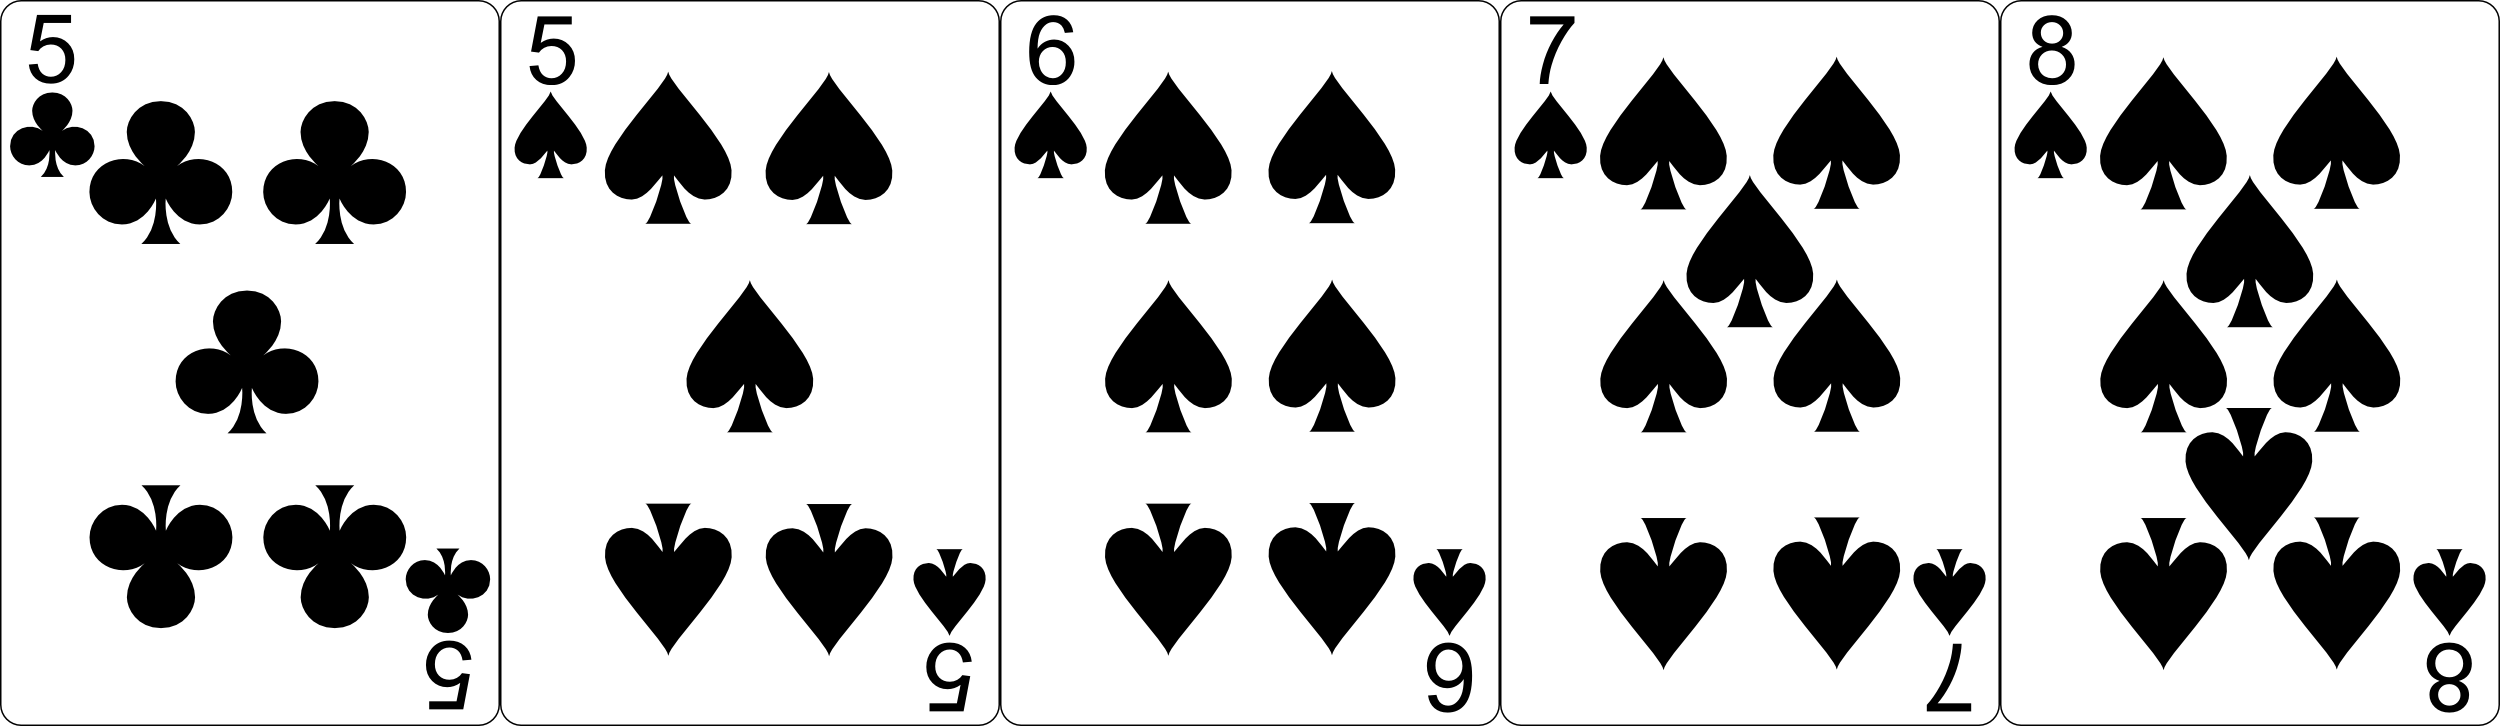
\includegraphics[width=\textwidth]{../img/w05-hands/pair.png}
 \end{minipage}
 \begin{minipage}[c]{\CardCaptionWidth}
  \caption{Par: två kort har samma valör.}
   \label{lab:shuffle:first-picture}
 \end{minipage}
\end{figure}

\begin{figure}[H]
 \begin{minipage}[c]{\CardWidth}
  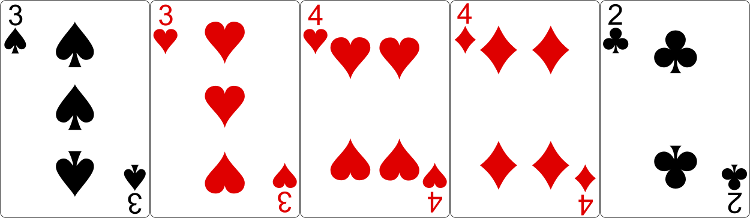
\includegraphics[width=\textwidth]{../img/w05-hands/twopair.png}
 \end{minipage}
 \begin{minipage}[c]{\CardCaptionWidth}
  \caption{Två par: handen har två \emph{olika} par.}
 \end{minipage}
\end{figure}

\begin{figure}[H]
 \begin{minipage}[c]{\CardWidth}
  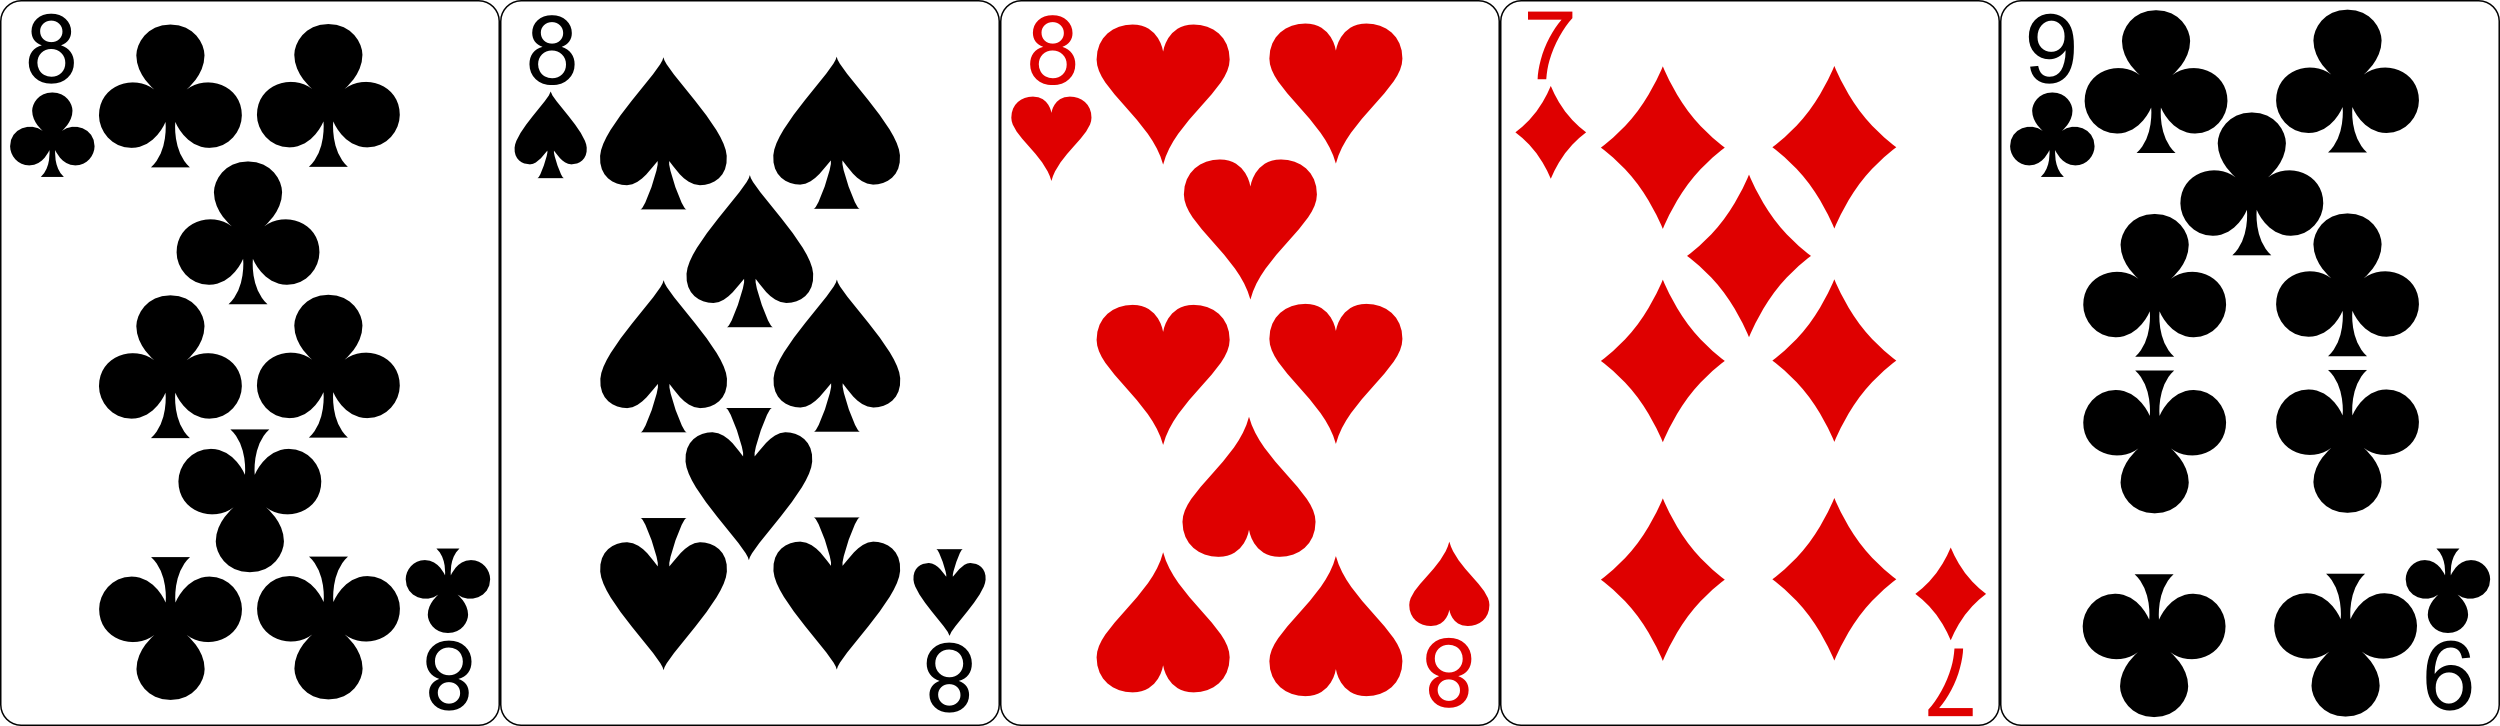
\includegraphics[width=\textwidth]{../img/w05-hands/trips.png}
 \end{minipage}
 \begin{minipage}[c]{\CardCaptionWidth}
  \caption{Triss: tre kort har samma valör.}
 \end{minipage}
\end{figure}

\begin{figure}[H]
 \begin{minipage}[c]{\CardWidth}
  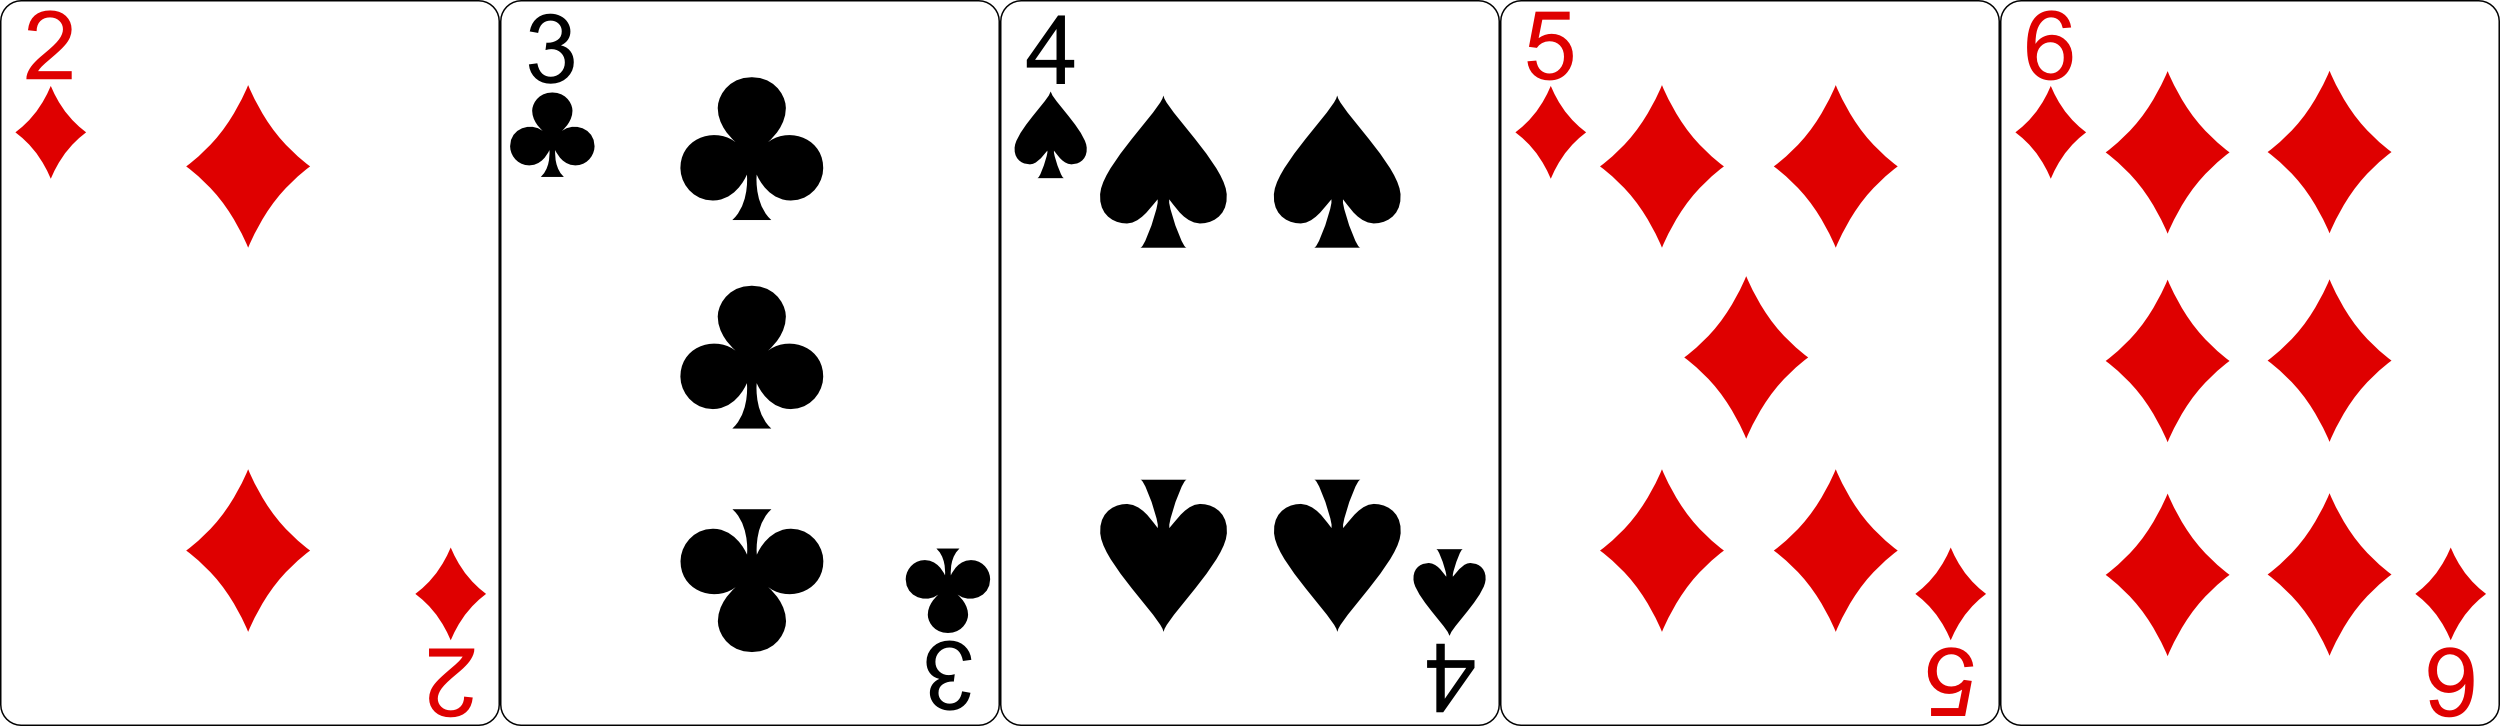
\includegraphics[width=\textwidth]{../img/w05-hands/straight.png}
 \end{minipage}
 \begin{minipage}[c]{\CardCaptionWidth}
  \caption{Stege: kortens valörer bildar en följd, ess kan vara antingen 1 eller 14.}
 \end{minipage}
\end{figure}

\begin{figure}[H]
 \begin{minipage}[c]{\CardWidth}
  \includegraphics[width=\textwidth]{../img/w05-hands/flush.png}
 \end{minipage}
 \begin{minipage}[c]{\CardCaptionWidth}
  \caption{Färg: alla kort har samma färg.}
 \end{minipage}
\end{figure}

\begin{figure}[H]
 \begin{minipage}[c]{\CardWidth}
  \includegraphics[width=\textwidth]{../img/w05-hands/fullhouse.png}
 \end{minipage}
 \begin{minipage}[c]{\CardCaptionWidth}
  \caption{Kåk: både triss och par.}
 \end{minipage}
\end{figure}

\begin{figure}[H]
 \begin{minipage}[c]{\CardWidth}
  \includegraphics[width=\textwidth]{../img/w05-hands/fours.png}
 \end{minipage}
 \begin{minipage}[c]{\CardCaptionWidth}
  \caption{Fyrtal: fyra kort har samma valör.}
 \end{minipage}
\end{figure}

\begin{figure}[H]
 \begin{minipage}[c]{\CardWidth}
  \includegraphics[width=\textwidth]{../img/w05-hands/straightflush.png}
 \end{minipage}
 \begin{minipage}[c]{\CardCaptionWidth}
  \caption{Färgstege: både stege och färg.}
 \end{minipage}
\end{figure}

\begin{figure}[H]
 \begin{minipage}[c]{\CardWidth}
  \includegraphics[width=\textwidth]{../img/w05-hands/none.png}
 \end{minipage}
 \begin{minipage}[c]{\CardCaptionWidth}
  \caption{Högt kort: inget mönster finns.}
 \label{lab:shuffle:last-picture}
  \end{minipage}
\end{figure}



\part{Appendix}
\appendix
%!TEX encoding = UTF-8 Unicode
%!TEX root = ../compendium2.tex

\chapter{Kojo}\label{appendix:kojo}

\section{Vad är Kojo?}

Kojo%
\footnote{\href{https://en.wikipedia.org/wiki/Kojo_(programming_language)}{en.wikipedia.org/wiki/Kojo\_(programming\_language)}}
 är en integrerad utvecklingsmiljö för Scala som är speciellt anpassad för programmeringsundervisning i grundskolan. Kojo används i LTH:s Science Center Vattenhallen för utbildning av grundskolelärare i programmering och vid skolbesök och annan besöksverksamhet, i vilken lärare och studenter vid LTH arbetar som handledare. 
 
 Kojo är öppen källkod och utvecklingsgemenskapen leds av Lalit Pant från Indien. I Kojo finns även lättillgängliga bibliotek som gör tröskeln lägre att programmera rörlig grafik och enkla spel.

Under kursens första laboration använder vi grafikbiblioteket i Kojo för att illustrera grundläggande begrepp, så som sekvens, alternativ, repetition och abstraktion.  


\begin{figure}[H]
\centering
\includegraphics[width=0.8\textwidth]{../img/kojo/kojo.png}
\caption{Den nybörjarvänliga utvecklingsmiljön Kojo för Scala på svenska.}
\label{fig:appendix:ide:kojo}
\end{figure}

\section{Använda grafikbiblioteket i Kojo}\label{appendix:ide:kojo:install}

Kojo bygger på den beprövade pedagogiska idén med sköldpaddsgrafik \Eng{turtle graphics}\footnote{\url{https://en.wikipedia.org/wiki/Turtle_graphics}}, där du skriver program som styr en sköldpadda med en penna under magen. När sköldpaddan rör sig bildas ett streck av valfri färg på skärmen. Beroende på hur du bestämmer att sköldpaddan ska röra sig och vilken färg du bestämmer att pennan ska ha, kan du skapa olika intressanta bilder och samtidigt lära dig om programmeringens grunder.

Under kursens första laboration ska du använda grafikbiblioteket i Kojo tillsammans med editorn VS \code{code} och \code{scala-cli} i terminalen (se appendix \ref{appendix:terminal} och \ref{appendix:compile}). Ladda ner filen \texttt{kojo.scala} från \url{https://cs.lth.se/pgk/kojolib} och spara i en ny katalog med hjälp av din webbläsare, eller via dessa kommandon:

\begin{REPLnonum}
> mkdir w01-kojo
> cd w01-kojo
> curl -o kojolib.scala -sL https://cs.lth.se/pgk/kojolib
\end{REPLnonum}

Nu kan du starta Scala REPL och rita med Kojo så här:

\begin{REPLnonum}
> scala-cli repl .
Welcome to Scala 3.1.2 (17.0.2, Java OpenJDK 64-Bit Server VM).
Type in expressions for evaluation. Or try :help.
                                                                                                                               
scala> fram; höger; fram; vänster

\end{REPLnonum}

Du kan starta VS \code{code} i aktuellt bibliotek så här:
\begin{REPLnonum}
> code .
\end{REPLnonum}

Skriv nedan progam i VS \code{code} och spara det i samma katalog som den tidigare nedladdade filen, under ett nytt valfritt filnamn, t.ex. \code{rita.scala}:

\begin{Code}
@main def rita =
  fram; höger
  fram; vänster
\end{Code}

Kör ditt fristående program med:
\begin{REPLnonum}
> scala-cli run .
\end{REPLnonum}

Du ska nu få upp ett fönster som heter Kojo Canvas med en sköldpadda som ritat två streck. När du stänger fönstret så avslutas programmet. Prova fler sköldpaddsfunktioner enligt tabell \ref{table:kojo:functions}.

I stället för att ladda ned filen \code{kojolib.scala} så kan du placera dess innehåll på lämpligt ställe i ditt program enligt nedan. Observera att raden som börjar med \code{//> using lib} ska vara en enda lång rad utan radbrytningar. Raden med \code{export} gör Kojos kommandon tillgängliga utan prefix:
\begin{CodeSmall}[breaklines=true]
//> using scala "3"
//> using lib "net.kogics:kojo-lib:0.1.1,url=https://github.com/lunduniversity/introprog/releases/download/kojo-lib-0.1.1/kojo-lib-0.1.1.jar"

export net.kogics.kojo.Swedish.*, padda.*, CanvasAPI.*, TurtleAPI.*
\end{CodeSmall}


\noindent Scala-koden för den svenska paddans api finns här: \\
%\href{https://github.com/litan/kojo/blob/master/src/main/scala/net/kogics/kojo/lite/i18n/svInit.scala}{github.com/litan/kojo/blob/master/src/main/scala/net/kogics/kojo/lite/i18n/svInit.scala} \\
\href{https://github.com/litan/kojo-lib/blob/main/src/main/scala/net/kogics/kojo/i18n/Swedish.scala}{github.com/litan/kojo-lib/blob/main/src/main/scala/net/kogics/kojo/i18n/Swedish.scala}


%Kojo kräver (numera) \emph{inte} att \texttt{java} finns på din dator utan kommer med en egen JVM. 
%Eftersom du behöver tillgång till JDK i kursen, är det lika bra att installera hela JDK direkt (och inte bara JRE, så som beskrivs å länken ovan); se vidare hur du gör detta i avsnitt \ref{appendix:compile:install-jdk}.
%\href{http://www.kogics.net/kojo-download}{www.kogics.net/kojo-download}


{\small\renewcommand{\arraystretch}{1.4}
\begin{longtable}{@{}p{0.42\textwidth} p{0.55\textwidth}}

\caption{Ett urval av funktioner i Kojo. Se även \href{http://lth.se/programmera}{lth.se/programmera}}\label{table:kojo:functions}\\

\emph{Svenska/Engelska} & \emph{Vad händer?}  \\ \hline
\code|sudda| \newline \code|clear| & Ritfönstret suddas \\
\code|fram| \newline \code|forward()| & Paddan går framåt 25 steg. \\
\code|fram(100)| \newline \code|forward(100)| & Paddan går framåt 100 steg. \\
\code|höger| \newline \code|right(90)| & Paddan vrider sig 90 grader åt höger. \\
\code|höger(45)| \newline \code|right(45)| & Paddan vrider sig 45 grader åt höger. \\
\code|vänster| \newline \code|left(90)| & Paddan vrider sig 90 grader åt vänster. \\
\code|vänster(45)| \newline \code|left(45)| & Paddan vrider sig 45 grader åt vänster. \\
\code|hoppa| \newline \code|hop| & Paddan hoppar 25 steg utan att rita. \\
\code|hoppa(100)| \newline \code|hop(100)| & Paddan hoppar 100 steg utan att rita. \\
\code|hoppaTill(100, 200)| \newline \code|jumpTo(100, 200)| & Paddan hoppar till läget (100, 200) utan att rita. \\
\code|gåTill(100, 200)| \newline \code|moveTo(100, 200)| & Paddan vrider sig och går till läget (100, 200). \\
\code|hem| \newline \code|home| & Paddan går tillbaka till utgångsläget (0, 0). \\
\code|öster| \newline \code|setHeading(0)| & Paddan vrider sig så att nosen pekar åt höger. \\
\code|väster| \newline \code|setHeading(180)| & Paddan vrider sig så att nosen pekar åt vänster. \\
\code|norr| \newline \code|setHeading(90)| & Paddan vrider sig så att nosen pekar uppåt. \\
\code|söder| \newline \code|setHeading(-90)  | & Paddan vrider sig så att nosen pekar neråt. \\
\code|mot(100,200)| \newline \code|towards(100, 200)| & Paddan vrider sig så att nosen pekar mot läget (100, 200) \\
\code|sättVinkel(90)| \newline \code|setHeading(90)| & Paddan vrider nosen till vinkeln 90 grader. \\
\code|vinkel| \newline \code|heading| & Ger vinkelvärdet dit paddans nos pekar. \\
\code|sakta(5000)| \newline \code|setAnimationDelay(5000) | & Gör så att paddan ritar jättesakta. \\
\code|suddaUtdata| \newline \code|clearOutput| & Utdatafönstret suddas. \\
\code|utdata("hej")| \newline \code|println("hej")| & Skriver texten \texttt{hej} i utdatafönstret. \\
\code|val t = indata("Skriv")| \newline \code|val t = readln("Skriv:")| & Väntar på inmatning efter ledtexten \texttt{Skriv} och sparar den inmatade texten i t.  \\
\code|textstorlek(100)| \newline \code|setPenFontSize(100)| & Paddan skriver med jättestor text nästa gång du gör skriv. \\
\code|båge(100, 90)| \newline \code|arc(100, 90)| & Paddan ritar en båge med radie 100 och vinkel 90. \\
\code|cirkel(100)| \newline \code|circle(radie)| & Paddan ritar en cirkel med radie 100. \\
\code|synlig| \newline \code|visible| & Paddan blir synlig. \\
\code|osynlig| \newline \code|invisible| & Paddan blir osynlig. \\
\code|läge.x| \newline \code|position.x| & Ger paddans x-läge \\
\code|läge.y| \newline \code|position.y| & Ger paddans y-läge \\
\code|pennaNer| \newline \code|penDown| & Sätter ner paddans penna så att den ritar när den går. \\
\code|pennaUpp| \newline \code|penUp| & Lyfter upp paddans penna så att den INTE ritar när den går. \\
\code|pennanÄrNere| \newline \code|penIsDown| & Kollar om pennan är nere eller inte. \\
\code|färg(rosa)| \newline \code|setPenColor(pink)| & Sätter pennans färg till rosa. \\
\code|fyll(lila)| \newline \code|setFillColor(purple)| & Sätter ifyllnadsfärgen till lila. \\
\code|fyll(genomskinlig)| \newline \code|setFillColor(noColor)| & Gör så att paddan inte fyller i något när den ritar. \\
\code|bredd(20)| \newline \code|setPenThickness(20)| & Gör så att pennan får bredden 20. \\
\code|sparaStil| \newline \code|saveStyle| & Sparar pennans färg, bredd och fyllfärg. \\
\code|laddaStil| \newline \code|restoreStyle| & Laddar tidigare sparad färg, bredd och fyllfärg. \\
\code|sparaLägeRiktning| \newline \code|savePosHe| & Sparar pennans läge och riktning \\
\code|laddaLägeRiktning| \newline \code|restorePosHe| & Laddar tidigare sparad riktning och läge \\
\code|siktePå| \newline \code|beamsOn| & Sätter på siktet. \\
\code|sikteAv| \newline \code|beamsOff| & Stänger av siktet. \\
\code|bakgrund(svart)| \newline \code|setBackground(black)| & Bakgrundsfärgen blir svart. \\
\code|bakgrund2(grön,gul)| \newline \code|setBackgroundV(green, yellow)| & Bakgrund med övergång från grönt till gult. \\
\code|upprepa(4){fram; höger}| \newline \code|repeat(4){forward; right}| & Paddan går fram och svänger höger 4 gånger. \\
\code|avrunda(3.99)| & Avrundar 3.99 till 4.0 \\
\code|slumptal(100)| & Ger ett slumptal mellan 0 och 99. \\
\code|slumptalMedDecimaler(100)| & Ger ett slumptal mellan 0 och 99.99999999 \\
\code|systemtid| & Ger nuvarande systemklocka i sekunder. \\
\code|räknaTill(5000)| & Kollar hur lång tid det tar för din dator att räkna till 5000. \\


\end{longtable}
}%end small


\section{Kojo Desktop}

Kojo finns som fristående skrivbordsapplikation, kallad Kojo Desktop. Kojo Desktop innehåller en egen editor med syntaxfärgning för Scala, men fungerar ännu så länge bara för Scala 2. En av de synligaste skillnaderna mellan Scala 2 och Scala 3 är att klammerparenteser vid flerradiga funktioner är nödvändiga i Scala 2, medan Scala 3 har valfria klammerparenteser. Så om du använder Kojo Desktop behöver du komma ihåg att omgärda sekvenser av rader som hör ihop med \code|{| och \code|}|. 

Kojo Desktop är förinstallerat på LTH:s datorer och körs igång med terminalkommandot \texttt{kojo} eller via applikationsmenyn.  För instruktioner om hur du installerar Kojo Desktop på din egen dator se här: \href{http://www.lth.se/programmera/installera/}{lth.se/programmera/installera}

När du startar Kojo första gången, välj ''Svenska'' i språkmenyn och starta om Kojo. Därefter fungerar grafikfunktionerna på svenska enligt tabell \ref{table:kojo:functions}. När du startat om Kojo inställt på svenska ser programmet ut ungefär som i figur \ref{fig:appendix:ide:kojo} på sidan \pageref{fig:appendix:ide:kojo}.

Det finns ett antal användbara kortkommando som du hittar i menyerna i Kojo Desktop. Undersök speciellt Ctrl+Alt+Mellanslag som ger autokomplettering baserat på det du börjat skriva.

\section{Kojo i Webbläsaren}

En begränsad variant av Kojo finns tillgänglig för programmering direkt i din webbläsare här: \url{http://kojo.lu.se/}

När du trycker på play-knappen så kompileras din kod på en server till Javascript via ScalaJS och därefter körs Javascript-koden i din webbläsare. 
Kojo på webben är också ännu så länge begränsad till Scala 2 och kräver att du omgärdar sekvenser av rader som hör ihop med \code|{| och \code|}|.


\section{Mer om Kojo}

I detta dokument finns en enkel introduktion till Kojo: \\ ''Introduction to Kojo'' \url{http://www.kogics.net/kojo-ebooks#intro}

%!TEX encoding = UTF-8 Unicode
%!TEX root = ../compendium2.tex

\chapter{Terminalfönster}\label{appendix:terminal}

\section{Vad är ett terminalfönster?}

I ett terminalfönster kan man skriva kommandon som kör program och hanterar filer. När man programmerar använder man ofta terminalkommando för att kompilera och exekvera sina program.  
 
\subsubsection{Terminal i Linux}

    \begin{figure}[!b]
    \centering
    \includegraphics[width=1.0\textwidth]{../img/linux-terminal.png}
    \caption{Terminalfönster i Ubuntu öppnas med Ctrl+Alt+T.}
    \label{fig:terminal:linux}
    \end{figure}

I Ubuntu trycker du lättast \textbf{Ctrl+Alt+T} eller sök efter ''terminal'' i app-menyn.  Då öppnas ett fönster med en blinkande markör som visar att det är redo att ta emot dina textkommando. Ett exempel på kommando är \texttt{ls} som skriver ut en lista med filer i det aktuella biblioteket, så som visas i fig. \ref{fig:terminal:linux}.

Det som visas i ett terminalfönster sköts av ett \textbf{kommandoskal} \Eng{command shell}, som är redo att ta emot kommando efter en prompt som slutar med ett \texttt{\$}-tecken. När du skriver ett kommando och trycker Enter anropar kommandoskalet en kommandotolk som tolkar och utför dina kommandon. Om ett kommando inte kan tolkas, skrivs ett felmeddelande. 

Det finns många användbara kortkommando, varav de viktigaste visas i tabell \ref{fig:terminal:shortcuts}. Det är bra om du lär dig dessa kortkommandon utantill så att ditt arbete i terminalen går snabbt och smidigt.

\begin{table}[H]
\renewcommand{\arraystretch}{1.15}
\begin{tabular}{@{}r | l}
pil upp/ner & bläddra i kommandohistoriken \\
Tab & ''auto-complete'', fyll i resten baserat på vad du skrivit hittills \\
Tab Tab & två tryck på Tab listar flera alternativ, om så finnes \\
Ctrl+A & ''ahead'', flytta markören till början av raden \\
Ctrl+E & ''end'', flytta markören till slutet av raden \\
Ctrl+K & ''kill'', ta bort tecken från markören till radens slut\\
Ctrl+U & ''undo'', ta bort tecken från markören till början av raden \\
Ctrl+Y & ''yank'', sätt in det som senast togs bort\\
Ctrl+Z & ''zleep'', stoppa pågående process, skriv sedan \texttt{bg} för bakgrundskörning\\
Ctrl+L & rensa terminalfönstret\\
Ctrl+D & avsluta kommandoskalet \\
\end{tabular}
    \caption{Viktiga kortkommandon i Linux terminalfönster.}
    \label{fig:terminal:shortcuts}
\end{table}

\noindent Ctrl+C orsakar normalt ett avbrott av pågående process, men om du vill att Ctrl+C ska vara ''Copy'' som vanligt för att kopiera markerad text, kan du ställa om detta med terminalförnstrets  meny ''Edit $\rightarrow$ Keyboard Shortcuts'', eller liknande.




 
\subsubsection{PowerShell, Cmd och Linux i Microsoft Windows}
Microsoft Windows är inte Linux-baserat, men i kommandotolken \textbf{Powershell} finns alias definierade för några vanliga Linux-kommandon, inkluderat \texttt{ls}, \texttt{cd} och \texttt{pwd}. 
Du startar Powershell t.ex. genom att trycka på Windows-knappen och skriva \texttt{powershell}. 
Du kan också, medan du bläddrar bland filer, klicka på filnamnsraden överst i filbläddraren och skriva \texttt{powershell} och tryck Enter; då startas Powershell i aktuellt bibliotek. Ändra gärna typsnitt och bakgrundsfärg med hjälp av fönstrets menyer, så att det blir lättare för dig att läsa vad som skrivs.

Det finns även i Windows den ursprungliga kommandotolken \textbf{Cmd} med helt andra kommandon. Till exempel skriver man i Cmd kommandot \texttt{dir} i stället för \texttt{ls} för att lista filer. 

I Windows 10 kan du (numera, om du installerad senaste uppdateringarna av Windows) även köra Ubuntu-terminalen med hjälp av Windows Linux Subsystem (WSL). Se vidare här om hur du kan installera WSL under Windows 10: 

\url{https://ubuntu.com/wsl} 

Läs mer här: \href{https://www.omgubuntu.co.uk/2020/03/windows-10-linux-kernel-update}{www.omgubuntu.co.uk/2020/03/windows-10-linux-kernel-update}



\subsubsection{Terminal i Apple macOS/OS X}


Apple OS X och macOS är Unix-baserade operativsystem. De flesta vanliga terminalkommandon som fungerar i Linux fungerar också under Apple OS X och macOS. Du startar ett terminalfönster i Apples operativsystem genom att klicka på förstoringsglaset uppe till höger, skriva \texttt{terminal}, och trycka Enter.

\section{Vad är en path/sökväg?}\label{terminal:path}

När du skriver ett kommando i terminalen, eller kör vilket program som helst på din dator, behöver operativsystemet identifera i vilken fil programmets maskinkod ligger innan programmet kan köras. 

Lokaliseringen av filer sker med hjälp av en \textbf{sökväg} \Eng{path}, som anger en position i filsystemet. Ofta betraktas filsystemet som ett upp-och-ned-vänt träd, och kallas därför även ''filträdet''. Den ''översta'' positionen kallas ''rot'' \Eng{root} och betecknas med ett enkelt snedstreck \texttt{/}. Kataloger som ligger i kataloger utgör förgreningar i trädet. En sökväg pekar ut vägar genom trädet som behövs för att nå ''löven'', som utgörs av själva filerna.

Du kan se var ett program ligger i Linux med hjälp av kommandot \texttt{which} enligt nedan.\footnote{Skriv \texttt{ gcm ls } i Windows Powershell för motsvarighet till \texttt{ which ls } \\ Eller skriv \texttt{ New-Alias which get-command } för tillgång till kommandot \texttt{which} i Powershell. \\ \href{http://stackoverflow.com/questions/63805/equivalent-of-nix-which-command-in-powershell}{stackoverflow.com/questions/63805/equivalent-of-nix-which-command-in-powershell}} Listan med bibliotek i sökvägen avskiljs med snedstreck.
\begin{REPLnonum}
$ which java
/usr/lib/jvm/oracle_jdk8/bin/java
$ which ls
/bin/ls
\end{REPLnonum}

En sökväg kan vara \textbf{absolut} eller \textbf{relativ}. En absolut sökväg utgår från roten och visar hela vägen från rot till destination, t.ex. \texttt{/usr/bin/firefox}, medan en relativ sökväg utgår från aktuellt bibliotek (där du ''står'') och börjar \textit{inte} med ett snedstreck.

Alla operativsystem håller reda på en mängd olika sökvägar för att kunna hitta speciella filer i filträdet. Dessa sökvägar lagras i s.k. \textbf{miljövariabler} \Eng{environment variables}. Det finns en \textit{speciell} miljövariabel som heter kort och gott \textbf{PATH}, i vilken alla sökvägar till de program finns, som ska vara tillgängliga för din användaridentitet direkt för exekvering genom sina filnamn, \textit{utan} att man behöver ange absoluta sökvägar. 

Du kan i Linux se vad som ligger i din PATH med kommandot \code{ echo $PATH } medan man i Windows Powershell skriver \code{$env.Path} där det bara är första bokstaven som ska vara en versal. I Linux separeras biblioteken i sökvägen med kolon, medan Windows använder semikolon.

Ibland kan du behöva uppdatera din PATH för att program som du installerat och ska bli allmänt tillgängliga. Detta görs på lite olika sätt i olika operativsystem, för Linux se t.ex. här:
\href{http://stackoverflow.com/questions/14637979/how-to-permanently-set-path-on-linux}{stackoverflow.com/questions/14637979/how-to-permanently-set-path-on-linux}

När man anger sökvägar finns några tecken med speciell betydelse:

\begin{tabular}{r  p{0.8\textwidth}}
\code|~| & ''tilde'', din hemkatalog \\
\code|/| & ''slash'', snedstreck anger filträdets rot om det finns i början av sökvägen, men utgör biblioteksavskiljare inuti sökvägen \\
\code|.| & en punkt anger aktuellt bibliotek, där du ''står'' \\
\code|..| & två punkter anger ett steg ''upp'' i filträdet \\
\code|"| & omgärda en sökväg med citationstecken, först och sist, om den innehåller annat än engelska bokstäver, t.ex. blanktecken\\
\code|\ | & \textit{backslash+blanktecken} används för att beteckna mellanslag i sökvägar som \textit{inte} omgärdas av citationstecken\\
\end{tabular}

\section{Några viktiga terminalkommando}

I tabell \ref{fig:terminal:commands} finns en lista med några viktiga terminalkommando som är bra att lära sig utantill.

En introduktion till LTH:s datorer med exempel på hur du använder vanliga Linux-kommandon finns i denna skrift \url{http://www.ddg.lth.se/perf/unix/} som används i introduktionsveckan för nybörjare på datateknikprogrammet vid LTH.

På sajten \url{http://ss64.com/} finns en mer omfattande lista med användbara terminalkommando och tillhörande förklaringarför för Linux (Bash), Windows (Powershell, Cmd) och Apple OS X (Bash).  

\begin{table}[H]
\renewcommand{\arraystretch}{1.25}
   
\begin{tabular}{@{}r | l}
\texttt{ls} & lista filer i aktuellt bibliotek (alltså där du ''står'')\\
\texttt{ls} \textit{p}  & lista filer i biblioteket  \textit{p} \\
\texttt{ls -A} & lista alla filer i aktuellt bibliotek, även gömda \\
\texttt{man ls} & manual för kommandot \texttt{ls}; testa även \texttt{man} för andra kommandon! \\
\texttt{cd} \textit{p} & ''change directory'', ändra aktuellt bibliotek till \textit{p}\\
\texttt{pwd} & ''print working directory'', skriv ut sökväg för aktuellt bibliotek \\
\texttt{cp} \textit{p1 p2} & ''copy'', kopiera filen med path \textit{p1} till en ny fil kallad \textit{p2} \\
\texttt{mv} \textit{p1 p2} & ''move'', byt namn på filen \textit{p1} till \textit{p2}  \\
\texttt{rm} \textit{p} & ''remove'', ta bort filen \textit{p}\\
\texttt{rm -r} \textit{p} & ''remove recursive'', ta bort biblioteket \textit{p} med allt innehåll; var försiktig!\\
\texttt{mkdir} \textit{p} & ''make dir'', skapa ett nytt bibliotek \textit{p}\\
\texttt{cat} \textit{p1 p2}& ''concatenate'', skriv ut hela innehållet i en eller flera filer \textit{p1 p2 etc.}\\
\texttt{less} \textit{p}& skriv ut innehållet i filen \textit{p}, en skärm i taget\\
\texttt{wget} \textit{url}&ladda ner \textit{url}, t.ex. \texttt{ wget http://cs.lth.se/pgk/ws -o ws.zip}\\
\texttt{unzip} \textit{p}& packa upp \textit{p}, t.ex. \texttt{ unzip ws.zip}\\
\end{tabular}

    \caption{Några viktiga terminalkommando i Linux. Med \textit{p}, \textit{p1}, \textit{p2}, etc.  avses en absolut eller relativ sökväg \Eng{path}, se avsnitt \ref{terminal:path}.}
    \label{fig:terminal:commands}

\end{table}


%!TEX encoding = UTF-8 Unicode
%!TEX root = ../compendium.tex

\chapter{Kompilera och exekvera}\label{appendix:compile}

\section{Vad är en kompilator?}

En \textbf{kompilator} \Eng{compiler} är ett program som läser programtext och översätter den till exekverbar maskinkod, så som visas i figur \ref{fig:appendix:compiler}. Programtexten som kompileras kallas källkod och utgörs av text som följer reglerna för ett programmeringsspråk, till exempel Scala eller Java. 

\begin{figure}[H]
\centering
\begin{tikzpicture}[node distance=1.8cm, scale=1.5]
\node (input) [startstop] {\bf\sffamily Källkod};
\node(inptext) [right of=input, text width=2cm, xshift=1.5cm]{För\\människor};
\node (compile) [process, below of=input] {\bf\sffamily Kompilator};
%\node(explain) [right of=compile, text width=5cm, xshift=3.0cm]{Översätter från källkod till maskinkod};
\node (output) [startstop, below of=compile] {\bf\sffamily Maskinkod};
\node(outtext) [right of=output, text width=2cm, xshift=1.5cm]{För\\maskiner};
\draw [arrow] (input) -- (compile);
\draw [arrow] (compile) -- (output);
\end{tikzpicture}
    \caption{En kompilator översätter från källkod till maskinkod.}
    \label{fig:appendix:compiler}
\end{figure}




Vissa kompilatorer genererar kod som kan köras av en processor direkt, medan andra kompilatorer genererar ett mellanformat som tolkas under exekveringen. Det senare är fallet med Java och Scala, vilket möjliggör att programmet kan kompileras en gång för alla plattformar och sedan kan programmet köras på all de processorer till vilka en s.k. virtuell maskin för Java finns \Eng{Java Virtual Machine, JVM}. Den kod som genereras av en kompilator som kodgenererar för JVM kallas \textbf{bytekod}.

Om kompileringen inte lyckas skriver kompilatorn ut ett felmeddelande och ingen maskinkod genereras. Det är inte lätt att bygga en kompilator som ger bra felmeddelanden i alla lägen, men felmeddelandet ger oftast goda ledtrådar till felorsaken efter att man lärt sig tolka det programmeringsspråksspecifika vokabulär som kompilatorn använder.

Även om programmet kompilerar utan felmeddelande och genererar exekverbar maskinkod, är det vanligt att programmet ändå inte fungerar som det är tänkt. Ibland är det mucket svårt att lista ut vad problemet beror på och man kan behöver göra omfattande undersökningar av vad som händer under körningen, genom att t.ex. skriva ut olika variablers värden eller på annat sätt ändra koden och se vad som händer. Denna process kallas felsökning eller avlusning \Eng{debugging}, och är en väsentlig del av all systemutveckling. 

En uttömmande testning av ett större program, som kör programmets \textit{alla} möjliga exekveringsvägar, är i praktiken omöjlig att genomföra inom rimlig tid, då antalet kombinationsmöjligheter växer mycket snabbt med storleken på programmet. 
Därför är kompilatorn ett mycket viktigt hjälpmedel. Med hjälp av den analys och de kontroller som görs av kompilatorn kan många buggar, som annars vore mycket svåra att hitta, undvikas och åtgärdas i kompileringsfasen, redan \textit{innan} man exekverar programmet. 


\section{Java JDK}

Scala, Java och flera andra språk använder Java-plattformen som exekveringsmiljö. Om man inte bara vill köra program som andra har utvecklat, utan även utveckla egna program som fungerar i denna miljö, behöver man installera Java Develpment Kit (JDK). Detta utvecklingspaket innehåller flera delar, bland annat:

\begin{itemize}

\item Kompilatorn \texttt{javac} kompilerar Java-program till bytekod som lagras i klassfiler med filnamnsändelsen \texttt{.class}.

\item Exekveringsmiljön Java Runtime Enviroment (JRE) med kommandot \texttt{java} som drar igång den virtuella javamaskinen (Java Virtual Machine) som kan ladda och exekvera bytekod lagrade i klassfiler.

\item Programmet \texttt{jar} som packar ihop många sammanhörande klassfiler till en enda jar-fil som lätt kan distribueras via nätet och sedan köras med \texttt{java}-kommandot på alla maskiner med JRE. 

\item Programmet \texttt{javap} som läser klassfiler och skriver ut vad de innehåller i ett format som kan läsas av människor (ett sådant program kallas disassembler).

\item I JDK ingår också en mycket stor mängd färdiga programbibliotek med stöd för nätverkskommunikation, filhantering, grafik, kryptering och en massa annat som behövs när man bygger moderna system. 

\end{itemize}  

\noindent Du kan läsa mer om Java och dess historik här: \\
\href{https://en.wikipedia.org/wiki/Java_(programming_language)}{https://en.wikipedia.org/wiki/Java\_(programming\_language)}

\subsection{Kontrollera om du har JDK installerat}\label{appendix:compile:check-jdk}

Öppna ett terminalfönster (se appendix \ref{appendix:terminal}) och skriv (observera det avslutande c:et i \texttt{javac}):
\begin{REPLnonum}
javac -version
\end{REPLnonum}
Då ska ungefär följande skrivas ut (där siffran 101 kan vara något annat):
\begin{REPLnonum}
javac 1.8.0_101
\end{REPLnonum}
Om utskriften säger att javac saknas, installera JDK8 enl. nedan.

Du kanske redan har enbart Java Runtime Environment (JRE) installerad, men inte JDK. Då saknar du javakompilatorn javac m.m. och behöver installera JDK, se nedan. Du kan kolla om du har JRE genom att skriva \texttt{java -version} (alltså utan c efter java). Eller så har du redan JDK installerad men inte rätt bibliotek i din PATH; se vidare nedan ang. uppdatering av PATH.



\subsection{Installera JDK}\label{appendix:compile:install-jdk}

Det finns flera JDK-distributioner att välja mellan, varav Oracle JDK och Azul Zulu OpenJDK är två exempel. Oracle JDK har störst spridning och är förinstallerad på LTH:s datorer. För att installera JDK på din egen dator behöver du gå igen flera steg, som behöver anpassas efter det operativsystem du kör, enligt nedan. 
På kurshemsidan under ''Verktyg'' finns kompletterande instruktioner:  \url{http://cs.lth.se/pgk/verktyg} 


Din användaridentitet behöver ha administratörsrättigheter för att du ska kunna genomföra installationen.



\subsubsection{Linux} 
För Ubuntu: läs först noga igenom och följ sedan dessa instruktioner till punkt och pricka: \\ \href{http://www.webupd8.org/2012/09/install-oracle-java-8-in-ubuntu-via-ppa.html}{www.webupd8.org/2012/09/install-oracle-java-8-in-ubuntu-via-ppa.html}

För andra Linux-distributioner, kör detta i terminalen (funkar även i Ubuntu men du får med detta kommando inte Oracles aningen snabbare JVM): \\ \texttt{sudo apt-get install openjdk-8-jdk}

\subsubsection{Windows/macOS}

\begin{enumerate}
\item Installera senaste JDK från Oracle. Om du inte har installerat JDK förr på din dator så be gärna någon kurskamrat med erfarenhet av detta att assistera dig medan du följer stegen nedan. 

\begin{enumerate}
\item Surfa till Oracles hemsida för Java SE här: \\ \url{http://www.oracle.com/technetwork/java/javase/downloads/}

\item Klicka på rubriken ''Java SE 8u101 / 8u102'' och på nästa sida klicka på knappen ''Accept License Agreement'' i listan under rubriken ''Java SE Development Kit 8u101''. (Siffrorna 101 eller 102 kan vara annorlunda om senare versioner tillkommit.)

\item Välj rätt version av operativsystem (Windows x64 eller Mac OS X). Det är viktigt att du väljer x64, d.v.s 64-bitarsvarianten som gäller för alla moderna datorer.

\item Klicka på länken och en stor fil kommer laddas ner till din dator.

\item Installera när filen laddats färdigt. 

\end{enumerate}

\item Uppdatera PATH, så att du får tillgång till alla kommando i terminalen:
\begin{itemize}
\item För Windows görs detta enklast genom att ladda ner och sedan köra denna fil genom att dubbelklicka på den: \\ \url{https://github.com/lunduniversity/introprog/raw/master/tools/windows-jdk-set-path.bat}
\item För macOS, läs här: \\ \href{https://docs.oracle.com/javase/8/docs/technotes/guides/install/mac_jdk.html}{docs.oracle.com/javase/8/docs/technotes/guides/install/mac\_jdk.html}

\item Om något krånglar, be om hjälp. Om du vill veta mer om PATH-uppdatering för java, läs här:\\ \url{https://java.com/sv/download/help/path.xml} \\
Om du kör engelska menyer byt \texttt{sv} mot \texttt{en} i adressen ovan.  Du kan ta reda på vilken katalog som ska läggas in sist i din PATH efter ett semikolon genom att bläddra bland dina systemfiler och undersöka var JDK har installerats; i Windows antagligen något liknande detta (kolla exakt vilket versionsnummer du har): \code|C:\Program Files\Java\jdk1.8.0_101\bin|
\end{itemize}

\item Starta om datorn. Det är först efter att en ny användarinloggning initierats, som PATH-tilldelningen får effekt.

\item Kontrollera att \texttt{javac} fungerar enligt avsnitt \ref{appendix:compile:check-jdk}.
\end{enumerate}


\section{Scala}

Scala använder JDK som exekveringsmiljö, men erbjuder ytterligare verktyg specifika för Scala. I utvecklingspaketet för Scala ingår bl.a. kompilatorn \texttt{scalac} och även ett interaktivt kommandoskal kallat Scala REPL där du kan testa din Scala-kod rad för rad och se vad som händer direkt. 

De flesta av kursens övningar görs i Scala REPL, medan laborationerna kräver kompilering av lite större program.

Du hittar mer om Scalas historik och annan bakgrundsinformation här: \mbox{%
 \href{https://en.wikipedia.org/wiki/Scala_(programming_language)}{en.wikipedia.org/wiki/Scala\_(programming\_language)}
}

\subsection{Installera Scala}

Scala finns förinstallerat på LTH:s datorer. Du installerar Scala-kompilatorn och den interaktiva kodexperimentmiljön Scala REPL på din egen dator enligt nedan. 

\begin{enumerate}
\item Kontrollera att du har JDK installerad enligt avsnitt \ref{appendix:compile:check-jdk} och installera vid behov enligt avsnitt \ref{appendix:compile:install-jdk}.
\item Surfa till denna hemsida för nedladdning av Scala 2.11.8: \\ \url{http://scala-lang.org/download/2.11.8.html}
\item Klicka på ''Download'' av den variant som är relevant för ditt operativsystem och spara filen:

\begin{enumerate}
\item \textbf{Linux Ubuntu}: Filen heter \texttt{scala-2.11.8.deb} och installeras genom att dubbelklicka på filen eller via terminalkommandot:\\ \code{sudo apt install ~/Downloads/scala-2.11.8.deb} \\ anpassa sökvägen ovan efter var du sparade filen 
\item \textbf{Windows}: Filen heter \texttt{scala-2.11.8.msi} och installationen startas med ett dubbelklick. Följ instruktionerna. Installationsprogrammet uppdaterar även din PATH åt dig och allt bör fungera efter omstart.
\item \textbf{macOS}: Filen heter \texttt{scala-2.11.8.tgz} och kan packas upp på lämpligt ställe med terminalkommandot \texttt{tar -xvzf scala-2.11.8.tgz} och sedan är det underkatalogen \texttt{bin} som ska inkluderas i din PATH. \TODO klura ut säkraste rådet för path-uppdatering på mac.
\end{enumerate}
Kontrollera att terminalkommandot \texttt{scala} fungerar för att starta Scala REPL:
\end{enumerate}
\begin{REPLnonum}
$ scala
Welcome to Scala 2.11.8 (Java HotSpot(TM) 64-Bit Server VM, Java 1.8.0_101).
Type in expressions for evaluation. Or try :help.

scala> println("hej")
hej

scala>
\end{REPLnonum}
 

\subsection{Scala Read-Evaluate-Print-Loop (REPL)}\label{appendix:compile:REPL}

För många språk, t.ex. Scala och Python, finns det en interaktiv tolk som gör det möjligt att exekvera enstaka programrader och direkt se effekten. En sådan tolk kallas Read-Evaluate-Print-Loop eftersom den läser en rad i taget och översätter till maskinkod som körs direkt.    

\TODO Kortkommandon: Ctrl+K etc.

\TODO :paste








%%!TEX encoding = UTF-8 Unicode
%!TEX root = ../compendium.tex

\chapter{Virtuell maskin}\label{appendix:vbox}

\section{Vad är en virtuell maskin?}

Du kan köra alla kursens verktyg i en så kallad virtuell maskin (vm). Det är ett enkelt och säkert sätt att installera ett nytt operativsystem i en ''sandlåda'' som inte påverkar din dators ursprungliga operativsystem. 

\section{Installera kursens vm}
Det finns en virtuell maskin förberedd med alla verktyg som du behöver förinstallerade. Gör så här:
\begin{enumerate}
\item     Installera VirtualBox v5 här: \\ \url{https://www.virtualbox.org/wiki/Downloads}
\item     Ladda ner filen vbox.zip här: \\ \url{http://fileadmin.cs.lth.se/pgk/vbox.zip} \\ OBS! Då filen är på nästan 4GB kan nedladdningen ta mycket lång tid.
\item     Packa upp filen vbox.zip i biblioteket "VirtualBox VMs" som du fick i din hemkatalog när du installerade VirtualBox. Du får då 3 filer som heter något med "introprog-ubuntu-64bit".
\item     Kolla med hjälp av denna sida: \\ \url{https://md5file.com/calculator} \\ så att filen "introprog-ubuntu-64bit.vdi" har denna sha256-cheksumma: \\ --- ska-stå-checksumma-här-sen ---
\item     Öppna VirtualBox och lägg till maskinen introprog-ubuntu-64bit genom menyn ''add''.
\item     Starta maskinen.
\item     Öppna ett terminalfönster och skriv scala och du är igång och kan göra första övningen!
\end{enumerate}

\section{Vad innehåller kursens vm?}

Den virtuella maskinen kör Xubuntu 14.04 med fönstermiljön XFCE, vilket är samma miljö som E-husets linuxdatorer kör. 

I den virtuella maskinen finns detta förinstallerat:

\begin{itemize}
\item Java JDK 8
\item Scala 2.11.8
\item Kojo 2.4.08
\item Eclipse Mars.2 med ScalaIDE 4.3
\item gedit med syntaxfärgning för Scala och Java
\item git
\item sbt
\item Ammonite REPL
\end{itemize}  /TODO!!

\part{Lösningar}

\setcounter{chapter}{11} %L in \Alph
\renewcommand\thechapter{\Alph{chapter}}
\chapter{Lösningar till övningarna}\label{chapter:solutions}

\PreSolutionfalse

\let\QUESTBEGIN\ifPreSolution  % to mark formatting and numbering of exercises
\let\SOLUTION\else  % to mark solutions in the same file as questions
\let\QUESTEND\fi    % to mark end of exercise

%!TEX encoding = UTF-8 Unicode
%!TEX root = ../exercises.tex

\ifPreSolution
\Exercise{\ExeWeekONE}\label{exe:W01}

\begin{Goals}
%!TEX encoding = UTF-8 Unicode

\item Förstå vad som händer när satser exekveras och uttryck evalueras.
\item Förstå sekvens, alternativ och repetition.
\item Känna till literalerna för enkla värden, deras typer och omfång.
\item Kunna deklarera och använda variabler och tilldelning, samt kunna rita bilder av minnessituationen då variablers värden förändras.
\item Förstå skillnaden mellan olika numeriska typer, kunna omvandla mellan dessa och vara medveten om noggrannhetsproblem som kan uppstå.
\item Förstå booleska uttryck och värdena \code{true} och \code{false}, samt kunna förenkla booleska uttryck.
\item Förstå skillnaden mellan heltalsdivision och flyttalsdivision, samt användning av rest vid heltalsdivision.
\item Förstå precedensregler och användning av parenteser i uttryck.
\item Kunna använda \code{if}-satser och \code{if}-uttryck.
\item Kunna använda \code{for}-satser och \code{while}-satser.
\item Kunna använda \code{math.random()} för att generera slumptal i olika intervaller.
\item Kunna beskriva skillnader och likheter mellan en procedur och en funktion.

\end{Goals}

\begin{Preparations}
\item \StudyTheory{01}
\item Du behöver en dator med Scala och Kojo installerad, se appendix~\ref{appendix:compile} och  \ref{appendix:kojo}.
\end{Preparations}

\else

\ExerciseSolution{\ExeWeekONE}

\fi  %%% END \ifPreSolution


\BasicTasks




\WHAT{Para ihop begrepp med beskrivning.}

\QUESTBEGIN

\Task \what

\vspace{1em}\noindent Koppla varje begrepp med den (förenklade) beskrivning som passar bäst:

\begin{ConceptConnections}
  litteral & 1 & & A & kan inträffa medan programmet kör \\ 
  sträng & 2 & & B & att översätta kod till exekverbar form \\ 
  sats & 3 & & C & vid anrop beräknas ett returvärde \\ 
  uttryck & 4 & & D & decimaltal med begränsad noggrannhet \\ 
  funktion & 5 & & E & bra då antalet repetitioner är bestämt i förväg \\ 
  procedur & 6 & & F & en kodrad som gör något; kan särskiljas med semikolon \\ 
  exekveringsfel & 7 & & G & beskriver vad data kan användas till \\ 
  kompileringsfel & 8 & & H & antingen sann eller falsk \\ 
  abstrahera & 9 & & I & för att ändra en variabels värde \\ 
  kompilera & 10 & & J & kombinerar värden och funktioner till ett nytt värde \\ 
  typ & 11 & & K & en sekvens av tecken \\ 
  for-sats & 12 & & L & att införa nya begrepp som förenklar kodningen \\ 
  while-sats & 13 & & M & anger ett specifikt datavärde \\ 
  tilldelning & 14 & & N & kan inträffa innan exekveringen startat \\ 
  flyttal & 15 & & O & bra då antalet repetitioner ej är bestämt i förväg \\ 
  boolesk & 16 & & P & vid anrop sker (sido)effekt; returvärdet är tomt \\ 
\end{ConceptConnections}

\SOLUTION

\TaskSolved \what

\begin{ConceptConnections}
  litteral & 1 & ~~\Large$\leadsto$~~ &  D & anger ett specifikt datavärde \\ 
  sträng & 2 & ~~\Large$\leadsto$~~ &  G & en sekvens av tecken \\ 
  sats & 3 & ~~\Large$\leadsto$~~ &  F & en kodrad som gör något; kan särskiljas med semikolon \\ 
  uttryck & 4 & ~~\Large$\leadsto$~~ &  H & kombinerar värden och funktioner till ett nytt värde \\ 
  funktion & 5 & ~~\Large$\leadsto$~~ &  K & vid anrop beräknas ett returvärde \\ 
  procedur & 6 & ~~\Large$\leadsto$~~ &  J & vid anrop sker (sido)effekt; returvärdet är tomt \\ 
  exekveringsfel & 7 & ~~\Large$\leadsto$~~ &  N & kan inträffa medan programmet kör \\ 
  kompileringsfel & 8 & ~~\Large$\leadsto$~~ &  M & kan inträffa innan exekveringen startat \\ 
  abstrahera & 9 & ~~\Large$\leadsto$~~ &  A & att införa nya begrepp som förenklar kodningen \\ 
  kompilera & 10 & ~~\Large$\leadsto$~~ &  C & att översätta kod till exekverbar form \\ 
  typ & 11 & ~~\Large$\leadsto$~~ &  I & beskriver vad data kan användas till \\ 
  for-sats & 12 & ~~\Large$\leadsto$~~ &  O & bra då antalet repetitioner är bestämt i förväg \\ 
  while-sats & 13 & ~~\Large$\leadsto$~~ &  P & bra då antalet repetitioner ej är bestämt i förväg \\ 
  tilldelning & 14 & ~~\Large$\leadsto$~~ &  L & för att ändra en variabels värde \\ 
  flyttal & 15 & ~~\Large$\leadsto$~~ &  E & decimaltal med begränsad noggrannhet \\ 
  boolesk & 16 & ~~\Large$\leadsto$~~ &  B & antingen sann eller falsk \\ 
\end{ConceptConnections}

\QUESTEND






\WHAT{Utskrift i Scala REPL.}

\QUESTBEGIN

\Task \what

\vspace{1em}\noindent Starta Scala REPL \Eng{Read-Evaluate-Print-Loop}.

\begin{REPLnonum}
> scala
Welcome to Scala 3.0.1 (OpenJDK 64-Bit Server VM, Java 11.0.8).
Type in expressions for evaluation. Or try :help.
scala -version.
scala>
\end{REPLnonum}

\Subtask Skriv efter prompten \code{scala>} en sats som skriver ut en valfri (bruklig/knasig) hälsningsfras, genom anrop av proceduren \code{println} med något strängargument. Tryck på \textit{Enter} så att satsen kompileras och exekveras.

\Subtask Skriv samma sats igen (eller tryck pil-upp) men ''glöm bort'' att skriva högerparentesen efter argumentet innan du trycker på \textit{Enter}. Vad händer?

\begin{framed}
\noindent\emph{Tips inför fortsättningen:} Det finns många användbara kortkommandon och andra trix för att jobba snabbt i REPL. Be gärna någon som kan dessa trix att visa dig hur man kan jobba snabbare. Läs appendix \ref{appendix:compile:REPL} och prova sedan att kopiera och klistra in text. Använd piltangenterna för att bläddra i historiken, Ctrl+A för att komma till början av raden, Ctrl+K för att radera resten av raden, etc.
\end{framed}



\SOLUTION
\TaskSolved \what

\SubtaskSolved Till exempel:
\begin{REPLnonum}
scala> println("hejsan svejsan")
\end{REPLnonum}

\SubtaskSolved Om högerparentes fattas får man fortsätta skriva på nästa rad. Detta indikeras med vertikalstreck i början av varje ny rad:
\begin{REPLnonum}
scala> println("hejsan svejsan"
     | + "!"
     | )
hejsan svejsan!
\end{REPLnonum}

\QUESTEND



\WHAT{Konkatenering av strängar.}

\QUESTBEGIN

\Task \what

\Subtask Skriv ett uttryck som konkatenerar två strängar, t.ex. \code{"gurk"} och \code{"burk"}, med hjälp av operatorn \code{+} och studera resultatet. Vad har uttrycket för värde och typ? Vilken siffra står efter ordet \code{res} i variabeln som lagrar resultatet?

\Subtask Använd resultatet från konkateneringen, t.ex. \code{res0} (byt ev. ut \code{0}:an mot siffran efter \code{res} i utskriften från förra evalueringen), och skriv ett uttryck med hjälp av operatorn \code{*} som upprepar resultatet från förra deluppgiften 42 gånger.


\SOLUTION

\TaskSolved \what

\SubtaskSolved
\begin{REPLnonum}
scala> "gurk" + "burk"
res1: String = gurkburk
\end{REPLnonum}
värde: \code{"gurkburk"}, typ:  \code{String}

\SubtaskSolved
\begin{REPLnonum}
scala> res1 * 42
res2: String = gurkatomatgurkatomatgurkatomatgurkatomatgurkatomatgurkatomatgurkatomatgurkatomatgurkatomatgurkatomatgurkatomatgurkatomatgurkatomatgurkatomatgurkatomatgurkatomatgurkatomatgurkatomatgurkatomatgurkatomatgurkatomatgurkatomatgurkatomatgurkatomatgurkatomatgurkatomatgurkatomatgurkatomatgurkatomatgurkatomatgurkatomatgurkatomatgurkatomatgurkatomatgurkatomatgurkatomatgurkatomatgurkatomatgurkatomatgurkatomatgurkatomatgurkatomat
\end{REPLnonum}

\QUESTEND




\WHAT{När upptäcks felet?}

\QUESTBEGIN

\Task \what

\Subtask Vad har uttrycket \code{ "hej" * 3 } för typ och värde? Testa i REPL.

\Subtask Byt ut 3:an ovan mot ett så pass stort heltal så att minnet blir fullt. Hur börjar felmeddelandet? Är detta ett körtidsfel eller ett kompileringsfel?

\Subtask Välj ett värde på argumentet efter operatorn \code{*} så att ett typfel genereras. Hur börjar felmeddelandet? Är detta ett körtidsfel eller ett kompileringsfel?

\begin{framed}
\noindent\emph{Tips inför fortsättningen:} Gör gärna fel när du kodar så lär du dig mer! Träna på att tolka olika felmeddelanden och fråga någon om hjälp om du inte förstår. Kompilatorns utskrifter kan vara till stor hjälp, men är ibland kryptiska. Om du kör fast och inte kommer vidare själv så be om hjälp, \emph{men be om tips snarare än färdiga lösningar} så att du behåller initiativet själv och tar kontroll över nästa steg i ditt lärande.
\end{framed}


\SOLUTION

\TaskSolved \what

\SubtaskSolved Typ: \code{String}, värde: \code{"hejhejhej"}

\SubtaskSolved Körtiddsfel:
\begin{REPLnonum}
scala> "hej" * Int.MaxValue
java.lang.OutOfMemoryError: Java heap space
\end{REPLnonum}

\SubtaskSolved Kompileringsfel: (indikeras av texten \code{<console> ... error:})
\begin{REPLnonum}
scala> "hej" * true
<console>:12: error: type mismatch;
 found   : Boolean(true)
 required: Int
       "hej" * true
\end{REPLnonum}
Ett typfel innebär att kompilatorn inte kan få typerna att överensstämma i t.ex. ett funktionsanrop. I Scala får vi reda på typfel redan vid kompilering medan i andra språk (t.ex. Javascript) upptäcks sådana fel under exekveringen, i värsta fall genom svårhittade buggar som kanske först märks långt senare.

\QUESTEND




\WHAT{Litteraler och typer.}

\QUESTBEGIN

\Task \what

\Subtask Ta hjälp av REPL-kommadot \verb+:type+ (kan förkortas \code{:t}) vid behov för att para ihop nedan litteraler med rätt typ.

\begin{ConceptConnections}[0.35\textwidth]
  \code|1    | & 1 & & A & \code|Float  | \\ 
  \code|1L   | & 2 & & B & \code|Double | \\ 
  \code|1.0  | & 3 & & C & \code|Unit   | \\ 
  \code|1D   | & 4 & & D & \code|Int    | \\ 
  \code|1F   | & 5 & & E & \code|Boolean| \\ 
  \code|'1'  | & 6 & & F & \code|Long   | \\ 
  \code|"1"| & 7 & & G & \code|String | \\ 
  \code|true | & 8 & & H & \code|Double | \\ 
  \code|false| & 9 & & I & \code|Char   | \\ 
  \code|()   | & 10 & & J & \code|Boolean| \\ 
%\Connect{\code|1      |}  {\code|Int    |}
%\Connect{\code|1L     |}  {\code|Long   |}
%\Connect{\code|1.0    |}  {\code|Double |}
%\Connect{\code|1D     |}  {\code|Double |}
%\Connect{\code|1F     |}  {\code|Float  |}
%\Connect{\code|'1'    |}  {\code|Char   |}
%\Connect{\code|\"1\"  |}  {\code|String |}
%\Connect{\code|true   |}  {\code|Boolean|}
%\Connect{\code|false  |}  {\code|Boolean|}
%\Connect{\code|()     |}  {\code|Unit   |}
\end{ConceptConnections}

\Subtask Vad händer om du adderar 1 till det största möjliga värdet av typen \code{Int}?
\\\emph{Tips:} se snabbreferensen \footnote{\url{http://cs.lth.se/pgk/quickref/}} under rubriken ''The Scala type system'' avsnitt ''Methods on numbers''.

\Subtask Vad är skillnaden mellan typerna \code{Long} och \code{Int}?

\Subtask Vad är skillnaden mellan typerna \code{Double} och \code{Float}?


\SOLUTION

\TaskSolved \what

\SubtaskSolved

\begin{ConceptConnections}
  \code|1    | & 1 & ~~\Large$\leadsto$~~ &  C & \code|Int    | \\ 
  \code|1L   | & 2 & ~~\Large$\leadsto$~~ &  F & \code|Long   | \\ 
  \code|1.0  | & 3 & ~~\Large$\leadsto$~~ &  J & \code|Double | \\ 
  \code|1D   | & 4 & ~~\Large$\leadsto$~~ &  D & \code|Double | \\ 
  \code|1F   | & 5 & ~~\Large$\leadsto$~~ &  B & \code|Float  | \\ 
  \code|'1'  | & 6 & ~~\Large$\leadsto$~~ &  A & \code|Char   | \\ 
  \code|"1"| & 7 & ~~\Large$\leadsto$~~ &  E & \code|String | \\ 
  \code|true | & 8 & ~~\Large$\leadsto$~~ &  G & \code|Boolean| \\ 
  \code|false| & 9 & ~~\Large$\leadsto$~~ &  I & \code|Boolean| \\ 
  \code|()   | & 10 & ~~\Large$\leadsto$~~ &  H & \code|Unit   | \\ 
%\ConnectSolved{\code|1      |}  {\code|Int    |}
%\ConnectSolved{\code|1L     |}  {\code|Long   |}
%\ConnectSolved{\code|1.0    |}  {\code|Double |}
%\ConnectSolved{\code|1D     |}  {\code|Double |}
%\ConnectSolved{\code|1F     |}  {\code|Float  |}
%\ConnectSolved{\code|'1'    |}  {\code|Char   |}
%\ConnectSolved{\code|\"1\"  |}  {\code|String |}
%\ConnectSolved{\code|true   |}  {\code|Boolean|}
%\ConnectSolved{\code|false  |}  {\code|Boolean|}
\end{ConceptConnections}

\SubtaskSolved Värdet går över gränsen för vad som får plats i ett 32 bitars heltal och ''börjar om'' på det minsta möjliga heltalet \code{Int.MinValue} eftersom det är så binär aritmetik aritmetik med begränsat antal bitar fungerar i CPU:n.
\begin{REPL}
scala> Int.MaxValue + 1
res3: Int = -2147483648

scala> Int.MinValue
res4: Int = -2147483648
\end{REPL}

\SubtaskSolved Båda är heltal men \code{Long} kan representera större tal än \code{Int}.

\SubtaskSolved Båda är flyttal men \code{Double} har dubbel precision och kan representera större tal med fler decimaler.



\QUESTEND





\WHAT{Matematiska funktioner. Scaladoc.}

\QUESTBEGIN

\Task \what

\Subtask Antag att du har ett schackbräde med 64 rutor. Tänk dig att du börjar med att lägga ett enda riskorn på första rutan och sedan 
lägger dubbelt så många riskorn i en ny hög för varje efterföljande ruta: 1, 2, 4, 8, ...  etc. När du har gjort detta för alla rutor, 
hur många riskorn har du totalt lagt på schackbrädet?\footnote{\url{https://en.wikipedia.org/wiki/Wheat_and_chessboard_problem}}

\emph{Tips:} Du ska beräkna $2^{64} - 1$. Om du skriver \code{math.} i REPL och trycker TAB får du se inbyggda matematiska funktioner i Scalas standardbibliotek:
\begin{REPLnonum}
scala> math.    // Tryck TAB direkt efter punkten och betrakta listan
\end{REPLnonum}
Använd funktionen \code{math.pow} och lämpliga argument. Om du anger \code{math.pow} eller \code{math.pow()} utan argument får du se funktionshuvudet med 
parameterlistan.

Om du surfar till \url{http://www.scala-lang.org/api/current/} och skriver \code{math} i sökrutan och sedan, efter att du klickat på 
\textbf{\texttt{\small scala.math}}, skriver \textbf{\texttt{\small pow}} i rutan längre ner, så filtreras sidan och du hittar dokumentationen 
av \code{ def pow } som du kan klicka på och läsa mer om.

\Subtask Definiera funktionen \code{omkrets} nedan i REPL. Går det bra att utelämna returtyp-annoteringen? Varför? Finns det anledning att ha den kvar?
\begin{Code}
def omkrets(radie: Double): Double = 2 * math.Pi * radie
\end{Code}

\Subtask Jordens (genomsnittliga) diameter (vid ekvatorn) är ca $12 750$ $km$. Skriv ett uttryck som anropar funktionen \code{omkrets} ovan för att beräkna hur många kilometer per dag man ungefär måste färdas om man vill åka jorden runt på 80 dagar.

\SOLUTION

\TaskSolved \what

\SubtaskSolved Beräkning av $2^{64} - 1$ med \code{math.pow} enligt nedan ger ungefär $1.8 \cdot 10^{19}$
\begin{REPL}
scala> math.pow(2, 64) - 1
res0: Double = 1.8446744073709552E19
\end{REPL}

\SubtaskSolved Ja, returtyp-annoteringen \code{: Double} kan utelämnas.

\begin{itemize}
\item Varför kan returtyp utelämnas?\\Eftersom kompilatorns typhärledning kan härleda returtypen.
\item Varför kan man vilja utelämna den?\\Det blir kortare att skriva utan.
\item Anledningar att ange returtyp:
\begin{itemize}
\item  Med explicit returtyp får du hjälp av kompilatorn att redan under kompileringen kontrollera att uttrycket till höger om likhetstecknet har den typ som förväntas.

\item Genom att du anger returtypen explicit får de som enbart läser metodhuvudet (och inte implementationen)
 tydligt se vad som returneras.
\end{itemize}
\end{itemize}

\SubtaskSolved Ca $500$ $km$.
\begin{REPL}
scala> omkrets(12750 / 2) / 80
res0: Double = 500.6913291658733
\end{REPL}

\QUESTEND




\WHAT{Variabler och tilldelning. Förändringsbar och oföränderlig variabel.}

\QUESTBEGIN

\Task \what~

\Subtask Rita en \emph{ny} bild av datorns minne efter \emph{varje} exekverad rad 1--6 nedan. Varje bild ska visa alla variabler som finns i minnet och deras variabelnamn, typ och värde.

\begin{REPL}[numbers=left, numberstyle=\color{black}\ttfamily\scriptsize\selectfont]
scala> var a = 13
scala> val b = a + 1
scala> var c = (a + b) * 2.0
scala> b = 0
scala> a = 0
scala> c = c + 1
\end{REPL}
Efter första raden ser minnessituationen ut så här:

\MEM{a}{Int}{13}

\Subtask Varför blir det fel på rad 4? Är det ett kompileringsfel eller exekveringsfel? Hur lyder felmeddelandet?

\SOLUTION

\TaskSolved \what

\SubtaskSolved

\begin{tabular}{@{}l l l}
\MEM{{\it Efter rad 1:~~~~} a}{Int}{13}\\
\MEM{{\it Efter rad 2:~~~~} a}{Int}{13} & \MEM{b}{Int}{14}\\
\MEM{{\it Efter rad 3:~~~~} a}{Int}{13} & \MEM{b}{Int}{14} & \MEM{c}{Double}{54.0}\\
\MEM{{\it Efter rad 4:~~~~} a}{Int}{13} & \MEM{b}{Int}{14} & \MEM{c}{Double}{54.0}\\
\MEM{{\it Efter rad 5:~~~~} a}{Int}{0} & \MEM{b}{Int}{14} & \MEM{c}{Double}{54.0}\\
\MEM{{\it Efter rad 6:~~~~} a}{Int}{0} & \MEM{b}{Int}{14} & \MEM{c}{Double}{55.0}\\
\end{tabular}

\SubtaskSolved
Oföränderliga variabler deklareras med nyckelordet \code{val}. Det går inte att tilldela en oföränderlig variabel ett nytt värde; vid försök blir det kompileringsfel som lyder \texttt{\textbf{error: reassignment to val}}. Kompileringsfel känns igen med hjälp av texten \texttt{\textbf{error:}}, så som visas nedan:
\begin{REPLnonum}
scala> b = 0
<console>:12: error: reassignment to val
       b = 0
         ^
\end{REPLnonum}

\QUESTEND


\WHAT{Slumptal med \code{math.random()}.}

\QUESTBEGIN

\Task\label{exercise:expressions:roll} \what

\Subtask Vad ger funktionen \code{math.random()} för resultatvärde? Vilken typ? Vad är största och minsta möjliga värde?
\\\emph{Tips:} Se scaladoc här: \Scaladoc och prova i REPL.

\Subtask Deklarera den parameterlösa funktionen \code{def roll: Int = ???} som ska representera ett tärningskast och ge ett slumpmässigt heltal mellan 1 och 6. Testa funktionen genom att anropa den många gånger. \\\emph{Tips:} Använd \code{math.random()} och multiplicera och addera med lämpliga heltal. Omge beräkningen med parenteser och avsluta med \code{.toInt} för att avkorta decimaler och omvandla typen från \code{Double} till \code{Int}.

\SOLUTION

\TaskSolved \what

\SubtaskSolved Ur dokumentationen:
\begin{Code}
/** Returns a Double value with a positive sign,
 *  greater than or equal to 0.0 and less than 1.0.
 */
def random(): Double
\end{Code}
Dokumentationskommentarer, som börjar med \code{/**} och slutar med \code{*/}, ger oss en beskrivning av hur funktionen fungerar. Efter dokumentationskommentaren kommer funktionshuvudet, som här berättar att funktionen heter \code{random} och alltid kommer att returnera en \code{Double}. (Verktyget \code{scaladoc} kan med hjälp av  dokumentationskommentarerna automatiskt generera webbsajter med speciella  dokumentationssidor och sökfunktioner.)

\SubtaskSolved
\begin{REPL}
scala> def roll: Int = (math.random() * 6 + 1).toInt

scala> roll
res0: Int = 4

scala> roll
res1: Int = 1
\end{REPL}

\QUESTEND




\WHAT{Repetition med \code{for}, \code{foreach} och \code{while}.}

\QUESTBEGIN

\Task \what

\Subtask Så här kan en \code{for}-sats ser ut:
\begin{Code}
for i <- 1 to 10 do print(s"$i, ")
\end{Code}
Använd en \code{for}-sats för att skriva ut resultatet av 100 tärningskast med funktionen \code{roll} från uppgift \ref{exercise:expressions:roll}.

\Subtask Så här kan en \code{foreach}-sats ser ut:
\begin{Code}
(1 to 10).foreach(i => print(s"$i, "))
\end{Code}
Använd en \code{foreach}-sats för att skriva ut resultatet av 100 tärningskast med funktionen \code{roll} från uppgift \ref{exercise:expressions:roll}.

\Subtask Så här kan en \code{while}-sats se ut:
\begin{Code}
var i = 1
while i <= 10 do { print(s"$i, "); i = i + 1 }
\end{Code}
Använd en \code{while}-sats för att skriva ut resultatet av 100 tärningskast med funktionen \code{roll} från uppgift \ref{exercise:expressions:roll}. Vad händer om du glömmer \code{i = i + 1} ?


\SOLUTION

\TaskSolved \what

\SubtaskSolved
\begin{Code}
for i <- 1 to 100 do print(s"$roll, ")
\end{Code}

\SubtaskSolved
\begin{Code}
(1 to 100).foreach(i => print(s"$roll, "))
\end{Code}


\SubtaskSolved
\begin{Code}
var i = 1
while i <= 100 do { print(s"$roll, "); i = i + 1 }
\end{Code}

\begin{Code}
var i = 1
while i <= 100 do
    print(s"$roll, ") 
    i += 1
\end{Code}




\QUESTEND






\WHAT{Alternativ med \code{if}-sats och \code{if}-uttryck.}

\QUESTBEGIN

\Task \what

\Subtask Så här kan en \code{if}-sats se ut (notera dubbla likhetstecken):
\begin{Code}
if roll == 3 then println("TRE") else println("INTE TRE")
\end{Code}
Testa ovan i REPL. Skriv sedan en \code{for}-sats som kastar 100 tärningar och skriver ut strängen \code{"GRATTIS! "} om det blir en sexa, annars en ledsen smiley: \code{":("}

\Subtask Så här kan ett \code{if}-uttryck se ut:
\begin{Code}
if roll < 6 then 0 else 1
\end{Code}
Testa ovan i REPL. Skriv sedan en \code{while}-sats som kastar 100 tärningar och räknar antalet sexor. Skriv ut antalet efter \code{while}-satsen.

\SOLUTION

\TaskSolved \what

\SubtaskSolved
\begin{Code}
for i <- 1 to 100 do 
  if roll == 6 then print("GRATTIS! ") else print(":(")
\end{Code}
eller
\begin{Code}
for (i <- 1 to 100) if (roll == 6) print("GRATTIS! ") else print(":(")
\end{Code}

\SubtaskSolved
\begin{Code}
var i = 1
var n = 0
while i <= 100 do
  if roll == 6 then n = n + 1
  i = i + 1
println("Antalet sexor: " + n)
\end{Code}


\QUESTEND



\WHAT{Sekvens, sats och block.}

\QUESTBEGIN

\Task \what

\Subtask Vad gör dessa satser?
\begin{REPLnonum}
scala> def p = { print("san"); print("!"); println("hej")}
scala> p;p;p;p
\end{REPLnonum}

\Subtask
Använd pil-upp för att få tillbaka raden du skrev med definitionen av proceduren \code{p}. Byt plats på strängarna i utskriftsanropen i proceduren \code{p} så att utskriften blir:
\begin{REPLnonum}
hejsan!
hejsan!
hejsan!
hejsan!
\end{REPLnonum}

\Subtask Hur tolkar kompilatorn klammerparenteser och semikolon? Vad är ett block?

\SOLUTION

\TaskSolved \what

\SubtaskSolved
Satserna skapar denna utskrift:
\begin{REPLnonum}
san!hej
san!hej
san!hej
san!hej
\end{REPLnonum}

\SubtaskSolved
\begin{REPLnonum}
scala> def p = { print("hej"); print("san"); println("!")}
scala> p;p;p;p
\end{REPLnonum}

\SubtaskSolved
\begin{itemize}
\item Klammerparenteser används för att gruppera flera satser. 
Klammerparenteser behövs om man vill definiera en funktion som består av mer än en sats. 
Sedan scala 3 kan man istället använda indentering för att definera en funktion med flera rader och satser.

\item Semikolon särskiljer flera satser. Semikolon behövs om man vill skriva många satser på samma rad.


\end{itemize}

\QUESTEND




\WHAT{Heltalsdivision.}

\QUESTBEGIN

\Task \what~Vilket värde och vilken typ hör till vilket uttryck?  Är du osäker på svaret, testa i REPL.

\begin{ConceptConnections}[0.3\textwidth]
  \code| 4 / 42      | & 1 & & A & \code|    4: Int      | \\ 
  \code| 42.0 / 2    | & 2 & & B & \code|   10: Int      | \\ 
  \code| 42 / 4      | & 3 & & C & \code| 21.0: Double   | \\ 
  \code| 42 % 4      | & 4 & & D & \code|true : Boolean  | \\ 
  \code| 4 % 42      | & 5 & & E & \code|false: Boolean  | \\ 
  \code| 40 % 4 == 0 | & 6 & & F & \code|    0: Int      | \\ 
  \code| 42 % 4 == 0 | & 7 & & G & \code|    2: Int      | \\ 
\end{ConceptConnections}

\SOLUTION

\TaskSolved \what

\begin{ConceptConnections}[0.3\textwidth]
  \code| 4 / 42      | & 1 & ~~\Large$\leadsto$~~ &  D & \code|    0: Int      | \\ 
  \code| 42.0 / 2    | & 2 & ~~\Large$\leadsto$~~ &  A & \code| 10.5: Double   | \\ 
  \code| 42 / 4      | & 3 & ~~\Large$\leadsto$~~ &  C & \code|   10: Int      | \\ 
  \code| 42 % 4      | & 4 & ~~\Large$\leadsto$~~ &  E & \code|    2: Int      | \\ 
  \code| 4 % 42      | & 5 & ~~\Large$\leadsto$~~ &  B & \code|    4: Int      | \\ 
  \code| 40 % 4 == 0 | & 6 & ~~\Large$\leadsto$~~ &  G & \code|true : Boolean  | \\ 
  \code| 42 % 4 == 0 | & 7 & ~~\Large$\leadsto$~~ &  F & \code|false: Boolean  | \\ 
\end{ConceptConnections}

\QUESTEND





\WHAT{Booleska värden.}

\QUESTBEGIN

\Task \what~Vilket värde har dessa uttryck?  % Uppgift 13

\Subtask \code{true && true}

\Subtask \code{false && true}

\Subtask \code{true || true}

\Subtask \code{false || true}


\Subtask \code{false || false}

\Subtask \code{true == true}

\Subtask \code{true != false}


\Subtask \code{true > false}

\Subtask \code{true && (1 / 0 > 1)}

\Subtask \code{false && (1 / 0 > 1)}

\SOLUTION

\TaskSolved \what

\SubtaskSolved \code{true}

\SubtaskSolved \code{false}

\SubtaskSolved \code{true}

\SubtaskSolved \code{true}


\SubtaskSolved \code{false}

\SubtaskSolved \code{true}

\SubtaskSolved \code{true}


\SubtaskSolved \code{true}

\SubtaskSolved Undantag kastas: \code{java.lang.ArithmeticException: / by zero}

\SubtaskSolved \code{false}

\QUESTEND





\WHAT{Booleska variabler.}

\QUESTBEGIN

\Task \what~Vad skrivs ut på rad 2 och 4 nedan?

\begin{REPL}
scala> var monster = false
scala> if monster then println("akta dig!!!")
scala> monster = true
scala> if monster then println("akta dig!!!")
\end{REPL}

\SOLUTION

\TaskSolved \what

\begin{itemize}
\item[2:] Ingenting skrivs ut.
\item[4:] \code{akta dig!!!}
\end{itemize}


\QUESTEND






\WHAT{Turtle graphics med Kojo.}

\QUESTBEGIN

\Task \what~På veckans laboration ska du använda Kojo för att verifiera att du kan använda sekvens, alternativ, repetition och abstraktion. Med Kojo ska du skapa Scala-program som ritar färgglada figurer med hjälp av ett lättanvänt Scala-bibliotek för \emph{turtle graphics}\footnote{\url{https://en.wikipedia.org/wiki/Turtle_graphics}}.

Starta Kojo (se appendix \ref{appendix:kojo}). Om du inte redan har svenska menyer: välj svenska i språkmenyn och starta om Kojo.  Skriv in nedan program och tryck på den \emph{gröna} play-knappen. Notera kopplingen mellan satssekvensen och vad som händer i ritfönstret.

\begin{Code}
sudda

fram; höger
fram; vänster
färg(grön)
fram
\end{Code}
\noindent


\Subtask Vad händer om du \emph{inte} börjar programmet med \code{sudda} och kör samma program upprepade gånger? Varför är det bra att börja programmet med \code{sudda}?

\Subtask Skriv kod som ritar en kvadrat enligt bilden nedan.
\vspace{1em}\\\includegraphics[width=0.47\textwidth]{../img/kojo/kvadrat}

\noindent Prova gärna olika sätt att skriva din kod \emph{utan} att resultatet ändras: skriv satser i sekvens på flera rader eller satser i sekvens på samma rad med semikolon emellan; använd blanktecken och blanka rader i koden. Hur vill du gruppera dina satser så att de är lätta för en människa att läsa?
%Prova att ändra på \emph{ordningen} mellan satserna och studera hur resultatet påverkas. Använd den \emph{gula} play-knappen  (programspårning) för att studera exekveringen i detalj. Vad händer du klickar på satser i ditt program och på rutor i programspårningen?


\Subtask Rita en trappa enligt bilden nedan.

\includegraphics[width=0.3\textwidth]{../img/kojo/stairs}

\Subtask Rita valfri bild på valfri bakgrund med hjälp av några av procedurerna i tabellen nedan. Du kan till exempel rita en rosa triangel med lila konturer mot svart bakgrund. % \ref{lab:kojo:kojo-procedures}.
Försök att underlätta läsbarheten av din kod med hjälp av lämpliga radbrytningar och gruppering av satser.


\begin{table}[H]
\begin{longtable}{l l}\small
\code|fram(100)| & Paddan går framåt 100 steg (25 om argument saknas).\\
\code|färg(rosa)| & Sätter pennans färg till rosa. \\
\code|fyll(lila)| & Sätter ifyllnadsfärgen till lila. \\
\code|fyll(genomskinlig)| & Gör så att paddan \emph{inte} fyller i något när den ritar. \\
\code|bredd(20)| & Gör så att pennan får bredden 20. \\
\code|bakgrund(svart)| & Bakgrundsfärgen blir svart. \\
\code|bakgrund2(grön,gul)| & Bakgrund med övergång från grönt till gult. \\
\code|pennaNer|  & Sätter ner paddans penna så att den ritar när den går. \\
\code|pennaUpp|  & Sänker paddans penna så att den \emph{inte} ritar när den går. \\
\code|höger(45)|   & Paddan vrider sig 45 grader åt höger. \\
\code|vänster(45)| & Paddan vrider sig 45 grader åt vänster. \\
\code|hoppa|       & Paddan hoppar 25 steg utan att rita. \\
\code|hoppa(100)|  & Paddan hoppar 100 steg utan att rita. \\
\code|hoppaTill(100, 200)| & Paddan hoppar till läget (100, 200) utan att rita. \\
\code|gåTill(100, 200)|    & Paddan vrider sig och går till läget (100, 200). \\
\code|öster|   & Paddan vrider sig så att nosen pekar åt höger. \\
\code|väster|  & Paddan vrider sig så att nosen pekar åt vänster. \\
\code|norr|    & Paddan vrider sig så att nosen pekar uppåt. \\
\code|söder|   & Paddan vrider sig så att nosen pekar neråt. \\
\code|mot(100,200)|   & Paddan vrider sig så att nosen pekar mot läget (100, 200) \\
\code|sättVinkel(90)| & Paddan vrider nosen till vinkeln 90 grader. \\
\end{longtable}
%\label{lab:kojo:kojo-procedures}
%\caption{Några användbara procedurer i Kojo.}
\end{table}

\begin{framed}
\noindent\emph{Tips inför fortsättningen:} Ha gärna både REPL och Kojo igång samtidigt. Då kan du undersöka hur olika kodkonstruktioner fungerar i REPL, medan du stegvis skapar allt större program i editorn i Kojo. Detta sätt att jobba har du nytta av under resten av kursen, både om du använder en texteditor och kompilerar i terminalen, och om du använder en professionell integrerad utvecklingsmiljö. Oavsett vilka andra verktyg du kör är det användbart att ha REPL igång i ett eget fönster som hjälp i den kreativa processen, medan du jagar buggar och medan du lär dig nya koncept. Så fort du undrar hur något fungerar i Scala: fram med REPL och testa!
\end{framed}


\SOLUTION

\TaskSolved \what

\SubtaskSolved Genom att börja din Kojo-program med \code{sudda} så startar du exekveringen i samma utgångsläge: en tom rityta \Eng{canvas} där paddan pekar uppåt, pennan är nere och pennans färg är röd.  Då blir det lättare att resonera om vad programmet gör från början till slut, jämfört med om exekveringen beror på resultatet av tidigare exekveringar.


\SubtaskSolved
\begin{Code}
sudda

fram; vänster
fram; vänster
fram; vänster
fram; vänster
\end{Code}


\SubtaskSolved
\begin{Code}
sudda

fram; vänster
fram; höger

fram; vänster
fram; höger

fram; vänster
fram; höger

fram; vänster
\end{Code}


\QUESTEND









\clearpage

\ExtraTasks %%%%%%%%%%%%%%%%%% EXTRAUPPGIFTER



\WHAT{Typ och värde.}

\QUESTBEGIN

\Task \what~Vilket värde och vilken typ hör till vilket uttryck?  Är du osäker på svaret, testa i REPL.

\begin{ConceptConnections}[0.3\textwidth]
  \code|1.0 + 18          | & 1 & & A & \code|42.0: Double    | \\ 
  \code|(41 + 1).toDouble | & 2 & & B & \code|65: Int         | \\ 
  \code|1.042e42 + 1      | & 3 & & C & \code|19.0: Double    | \\ 
  \code|12E6.toLong       | & 4 & & D & \code|12000000: Long  | \\ 
  \code|32.toChar.toString| & 5 & & E & \code|'*': Char       | \\ 
  \code|'A'.toInt         | & 6 & & F & \code|48: Int         | \\ 
  \code|0.toInt           | & 7 & & G & \code|" ": String   | \\ 
  \code|'0'.toInt         | & 8 & & H & \code|1.042E42: Double| \\ 
  \code|'9'.toInt         | & 9 & & I & \code|'q': Char       | \\ 
  \code|'A' + '0'         | & 10 & & J & \code|113: Int        | \\ 
  \code|('A' + '0').toChar| & 11 & & K & \code|0: Int          | \\ 
  \code|"*!%#".charAt(0)| & 12 & & L & \code|57: Int         | \\ 
\end{ConceptConnections}

\SOLUTION

\TaskSolved \what

\begin{ConceptConnections}
  \code|1.0 + 18          | & 1 & ~~\Large$\leadsto$~~ &  E & \code|19.0: Double    | \\ 
  \code|(41 + 1).toDouble | & 2 & ~~\Large$\leadsto$~~ &  L & \code|42.0: Double    | \\ 
  \code|1.042e42 + 1      | & 3 & ~~\Large$\leadsto$~~ &  A & \code|1.042E42: Double| \\ 
  \code|12E6.toLong       | & 4 & ~~\Large$\leadsto$~~ &  K & \code|12000000: Long  | \\ 
  \code|32.toChar.toString| & 5 & ~~\Large$\leadsto$~~ &  G & \code|" ": String   | \\ 
  \code|'A'.toInt         | & 6 & ~~\Large$\leadsto$~~ &  H & \code|65: Int         | \\ 
  \code|0.toInt           | & 7 & ~~\Large$\leadsto$~~ &  I & \code|0: Int          | \\ 
  \code|'0'.toInt         | & 8 & ~~\Large$\leadsto$~~ &  F & \code|48: Int         | \\ 
  \code|'9'.toInt         | & 9 & ~~\Large$\leadsto$~~ &  D & \code|57: Int         | \\ 
  \code|'A' + '0'         | & 10 & ~~\Large$\leadsto$~~ &  B & \code|113: Int        | \\ 
  \code|('A' + '0').toChar| & 11 & ~~\Large$\leadsto$~~ &  J & \code|'q': Char       | \\ 
  \code|"*!%#".charAt(0)| & 12 & ~~\Large$\leadsto$~~ &  C & \code|'*': Char       | \\ 
\end{ConceptConnections}

%\Subtask \code{1.0 + 18}
%
%\Subtask \code{(41 + 1).toDouble}
%
%\Subtask \code{1.042e42 + 1}
%
%\Subtask \code{12E6.toLong}
%
%\Subtask \code{"gurk" + 'a'}
%
%\Subtask \code{32.toChar.toString}
%
%\Subtask \code{'A'.toInt}
%
%\Subtask \linebreak[0] \code{'0'.toInt}
%
%\Subtask \code{'0'.toInt}
%
%\Subtask \code{'9'.toInt}
%
%\Subtask \code{'A' + '0'}
%
%\Subtask \code{('A' + '0').toChar}
%
%\Subtask \code{"*!%#".charAt(0)}
%%%%%%%%%%%%%%%%%%%%%%%%%%%%%%%%%%%%%%%%%%%%%%%%
%\SubtaskSolved \code{Double, 19}
%
%\SubtaskSolved \code{Double, 42}
%
%\SubtaskSolved \code{Double, 1.042E42}
%
%\SubtaskSolved \code{Long, 12000000}
%
%\SubtaskSolved \code{String, gurka}
%
%\SubtaskSolved \code{String, " "}
%
%\SubtaskSolved \code{Int, 65}
%
%\SubtaskSolved \code{Int, 48}
%
%\SubtaskSolved \code{Int,49}
%
%\SubtaskSolved \code{Int,57}
%
%\SubtaskSolved \code{Int, 113}
%
%\SubtaskSolved \code{Char, 'q'}
%
%\SubtaskSolved \code{Char, '*'}


\QUESTEND




\WHAT{Satser och uttryck.}

\QUESTBEGIN

\Task \what

\Subtask Vad är det för skillnad på en sats och ett uttryck?

\Subtask Ge exempel på satser som inte är uttryck?

\Subtask Förklara vad som händer för varje evaluerad rad:
\begin{REPL}
scala> def värdeSaknas = ()
scala> värdeSaknas
scala> värdeSaknas.toString
scala> println(värdeSaknas)
scala> println(println("hej"))
\end{REPL}

\Subtask Vilken typ har literalen \code{()}?

\Subtask Vilken returtyp har \code{println}?

\SOLUTION

\TaskSolved \what

\SubtaskSolved  Ett utryck kan evalueras och resulterar då i ett användbart värde. En sats \emph{gör} något (t.ex. skriver ut något), men resulterat inte i något användbart värde.

\SubtaskSolved \code{println()}

\SubtaskSolved

 \code{värdeSaknas} innehåller Unit

 Skriver ut \code{Unit}

 Skriver ut \code{"()"}

 Skriver ut \code{"()"}

 Skriver först ut hej med det innersta anropet och sen \code{()} med det yttre anropet

\SubtaskSolved  \code{Unit}

\SubtaskSolved  \code{Unit}

\QUESTEND



\WHAT{Procedur med parameter.}

\QUESTBEGIN

\Task \what~En procedur är en funktion som orsakar en effekt, till exempel en utskrift eller en variabeltilldelning, men som inte returnerar något intressant resultatvärde.%
\footnote{I Scala är procedurer funktioner som returnerar det \emph{tomma värdet}, vilket skrivs \code{()} och är av typen \code{Unit}. I Java och flera andra språk finns inget tomt värde och man har en specialsyntax för procedurer som använder nyckelordet \code{void}. }

\Subtask Deklarera en förändringsbar variabel \code{highscore} som initieras till 0.

\Subtask Deklarera en procedur \code{updateHighscore} som tar en parameter \code{points} och tilldelar \code{highscore} ett nytt värde om \code{points} är större än \code{highscore} och skriver ut strängen \code{"REKORD!"}. Om inte \code{points} är större än \code{highscore} ska strängen \code{"GE INTE UPP!"} skrivas ut. Testa proceduren i REPL.

\Subtask Gör en ny variant av \code{updateHighscore}, som \emph{inte} är en procedur utan i stället är en funktion som ger en sträng för senare utskrift. Testa funktionen i REPL.

\SOLUTION

\TaskSolved \what

\SubtaskSolved
\begin{Code}
var highscore = 0
\end{Code}

\SubtaskSolved
\begin{Code}
def updateHighscore(points: Int): Unit =
  if points > highscore then
    highscore = points
    println("REKORD!")
  else println("GE INTE UPP!")
\end{Code}

\SubtaskSolved
\begin{Code}
def updateHighscore(points: Int): String =
  if points > highscore then
    highscore = points
    "REKORD!"
  else "GE INTE UPP!"
\end{Code}



\QUESTEND


\WHAT{Flyttalsaritmetik.}

\QUESTBEGIN

\Task \what

\Subtask Vilket är det minsta positiva värdet av typen \code{Double}?

\Subtask Vad är värdet av detta uttryck? Varför blir det så?
\begin{REPL}
scala> Double.MaxValue + Double.MinPositiveValue == Double.MaxValue
\end{REPL}

\SOLUTION

\TaskSolved \what

\SubtaskSolved

\begin{REPL}
scala> Double.MinPositiveValue
res0: Double = 4.9E-324
\end{REPL}

\SubtaskSolved

\begin{REPL}
scala> Double.MaxValue + Double.MinPositiveValue == Double.MaxValue
res2: Boolean = true
\end{REPL}

\QUESTEND



\WHAT{\code{if}\textit{-sats}.}

\QUESTBEGIN

\Task \what~För varje rad nedan, beskriv vad som skrivs ut.  % Uppgift 18
\begin{REPL}
scala> if !true then println("sant") else println("falskt")
scala> if !false then println("sant") else println("falskt")
scala> def singlaSlant = if math.random() < 0.5 then "krona" else "klave"
scala> for i <- 1 to 5 do print(s"$i:$singlaSlant ")
\end{REPL}

\SOLUTION

\TaskSolved \what

\begin{enumerate}
\item Utskrift: \code{falskt}
\item Utskrift: \code{sant}
\item Inget skrivs ut, funktionen deklareras men körs ej.
\item Utskrift: \code{1:krona 2:klave 3:krona 4:krona 5:klave } eller liknande beroende på vilka slumptal \code{math.random()} ger.
\end{enumerate}

\QUESTEND




\WHAT{\code{if}\textit{-uttryck}.}

\QUESTBEGIN

\Task  Deklarera följande variabler med nedan initialvärden:

\begin{REPLnonum}
scala> var grönsak = "gurka"
scala> var frukt = "banan"
\end{REPLnonum}

Ange för varje rad nedan vad uttrycket har för värde och typ:
\begin{REPLnonum}
scala> if grönsak == "tomat" then "gott" else "inte gott"
scala> if frukt == "banan" then "gott" else "inte gott"
scala> if true then grönsak else 42
scala> if false then grönsak else 42
\end{REPLnonum}

\SOLUTION


\TaskSolved \what~Notera typen \code{Any} på de sista två uttrycken.

\begin{REPLnonum}
scala> if grönsak == "tomat" then "gott" else "inte gott"
res0: String = inte gott

scala> if frukt == "banan" then "gott" else "inte gott"
res1: String = gott

scala> if true then grönsak else 42
res2: Any = gurka

scala> if false then grönsak else 42
res3: Any = 42
\end{REPLnonum}


\QUESTEND





\WHAT{Modulo-operatorn {\tt \%} och Booleska värden.}

\QUESTBEGIN

\Task \what

\Subtask Deklarera en funktion \code{def isEven(n: Int): Boolean = ???} som ger \code{true} om talet \code{n} är jämnt, annars \code{false}.

\Subtask Deklarera en funktion \code{def isOdd(n: Int): Boolean = ???} som ger \code{false} om talet \code{n} är jämnt, annars \code{true}.

\SOLUTION


\TaskSolved \what

\SubtaskSolved
\begin{REPL}
scala> def isEven(n: Int): Boolean = n % 2 == 0

scala> isEven(42)
res0: Boolean = true

scala> isEven(43)
res1: Boolean = false

\end{REPL}


\SubtaskSolved
\begin{REPL}
scala> def isOdd(n: Int): Boolean = !isEven(n)

scala> isOdd(42)
res2: Boolean = false

scala> isOdd(43)
res3: Boolean = true
\end{REPL}


\QUESTEND





\WHAT{Skillnader mellan \code{var}, \code{val}, \code{def}.}

\QUESTBEGIN

\Task \what~

\Subtask
 Evaluera varje rad en i taget i tur och ordning i Scala REPL. För varje rad nedan: förklara för vad som händer och notera värde och ev fel. % Uppgift 15
\begin{REPL}
scala> var x = 30
scala> x + 1
scala> x = x + 1
scala> x == x + 1
scala> val y = 20
scala> y = y + 1
scala> var z = { println("hej z!"); math.random() }
scala> def w = { println("hej w!"); math.random() }
scala> z
scala> z
scala> z = z + 1
scala> w
scala> w
scala> w = w + 1
\end{REPL}


\Subtask Vad är det för skillnad på \code{var}, \code{val} och \code{def}?



\SOLUTION

\TaskSolved \what

\SubtaskSolved
\begin{REPL}
  scala> var x = 30
  x: Int = 30

  scala> x + 1
  res6: Int = 31

  scala> x = x + 1
  x: Int = 31

  scala> x == x + 1
  res7: Boolean = false

  scala> val y = 20
  y: Int = 20

  scala> y = y + 1
  <console>:12: error: reassignment to val
         y = y + 1
           ^

  scala> var z = { println("hej z!"); math.random() }
  hej z!
  z: Double = 0.3381365875903367

  scala> def w = { println("hej w!"); math.random() }
  w: Double

  scala> z
  res8: Double = 0.3381365875903367

  scala> z
  res9: Double = 0.3381365875903367

  scala> z = z + 1
  z: Double = 1.3381365875903368

  scala> w
  hej w!
  res10: Double = 0.06420209879434557

  scala> w
  hej w!
  res11: Double = 0.5777951341051852

  scala> w = w + 1
  <console>:12: error: value w_= is not a member of object
         w = w + 1
\end{REPL}


\SubtaskSolved
\begin{itemize}
\item \code{var namn = uttryck} används för att deklarera en förändringsbar variabel. Namnet kan med hjälp av en tilldelningssats referera till nya värden.

\item \code{val namn = uttryck} används för att deklarera en oföränderlig variabel som efter initialisering inte kan förändras med tilldelningssatser. Vid försök ges kompileringsfel.
\item \code{def namn = uttryck} används för att deklarera en funktion vars uttryck evalueras varje gång den anropas.
\end{itemize}

\QUESTEND




\WHAT{Skillnaden mellan \code{if} och \code{while}.}

\QUESTBEGIN

\Task \what~Vad blir resultatet av rad 3 och 4?

\begin{REPL}
scala> def lotto1 = if math.random() > 0.5 then print("vinst :) ")
scala> def lotto2 = while math.random() > 0.5 do print("vinst :) ")
scala> lotto1
scala> lotto2
\end{REPL}

\SOLUTION

\TaskSolved \what

\begin{itemize}
\item Rad 3: Har du tur (50\% chans) får du vinst en gång.

\item Rad 4: Har du tur får du många vinster i rad. Sannolikheten för $n$ vinster i rad är $(\frac{1}{2})^n$.
\end{itemize}
\QUESTEND












\clearpage

\AdvancedTasks   %%%%%%%%%%%%%%%%%%% FÖRDJUPNINGSUPPGIFTER





\WHAT{Logik och De Morgans Lagar.}

\QUESTBEGIN

\Task \what~Förenkla följande uttryck. Antag att \code{poäng} och \code{highscore} är heltalsvariabler medan \code{klar} är av typen \code{Boolean}.
  % Uppgift 24

\Subtask \code{poäng > 100 && poäng > 1000}

\Subtask \code{poäng > 100 || poäng > 1000}

\Subtask \code{!(poäng > highscore)}

\Subtask \code{!(poäng > 0 && poäng < highscore) }

\Subtask \code{!(poäng < 0 || poäng > highscore) }

\Subtask \code{klar == true}

\Subtask \code{klar == false}

\SOLUTION

\TaskSolved \what


\SubtaskSolved \code{poäng > 1000}

\SubtaskSolved \code{poäng > 100}

\SubtaskSolved \code{poäng <= highscore}

\SubtaskSolved \code{poäng <= 0 || poäng >= highscore }

\SubtaskSolved \code{poäng >= 0 && poäng <= highscore}

\SubtaskSolved \code{klar}

\SubtaskSolved \code{!klar}


\QUESTEND






\WHAT{Stränginterpolatorn \code{s}.}

\QUESTBEGIN

\Task \what~Med ett \code{s} framför en strängliteral får man hjälp av kompilatorn att, på ett typsäkert sätt, infoga variabelvärden i en sträng.
Variablernas namn ska föregås med ett dollartecken , t.ex. \code{s"Hej $namn"}.
Om man vill evaluera ett uttryck placeras detta inom klammer direkt efter dollartecknet, t.ex.
\code/s"Dubbla längden: ${namn.size * 2}"/

\Subtask Vad skrivs ut nedan?
\begin{REPL}
scala> val f = "Kim"
scala> val e = "Finkodare"
scala> println(s"Namnet '$f $e' har ${f.size + e.size} bokstäver.")
\end{REPL}

\Subtask Skapa följande utskrifter med hjälp av stränginterpolatorn \code{s} och variablerna \code{f} och \code{e} i föregående deluppgift.
\begin{REPL}
Kim har 3 bokstäver.
Finkodare har 9 bokstäver.
\end{REPL}

\SOLUTION

\TaskSolved \what

\SubtaskSolved
\begin{REPLnonum}
Namnet 'Kim Finkodare' har 12 bokstäver.
\end{REPLnonum}

\SubtaskSolved
\begin{REPLnonum}
println(s"$f har  ${f.size} bokstäver.")
println(s"$e har  ${e.size} bokstäver.")
\end{REPLnonum}

\QUESTEND



\WHAT{Tilldelningsoperatorer.}

\QUESTBEGIN

\Task \what~Man kan förkorta en tilldelningssats som förändrar en variabel, t.ex. \code{x = x + 1}, genom att använda så kallade tilldelningsoperatorer och skriva \code{x += 1} som betyder samma sak. Rita en ny bild av datorns minne efter varje rad nedan. Bilderna ska visa variablers namn, typ och värde.

\begin{REPL}
scala> var a = 40
scala> var b = a + 40
scala> a += 10
scala> b -= 10
scala> a *= 2
scala> b /= 2
\end{REPL}

\SOLUTION

\TaskSolved \what

\begin{tabular}{l l}
\MEM{{\it Efter rad1:~~~~} a}{Int}{40}\\
\MEM{{\it Efter rad2:~~~~} a}{Int}{40} & \MEM{b}{Int}{80}\\
\MEM{{\it Efter rad3:~~~~} a}{Int}{50} & \MEM{b}{Int}{80}\\
\MEM{{\it Efter rad4:~~~~} a}{Int}{50} & \MEM{b}{Int}{70} \\
\MEM{{\it Efter rad5:~~~~} a}{Int}{100} & \MEM{b}{Int}{70} \\
\MEM{{\it Efter rad6:~~~~} a}{Int}{100} & \MEM{b}{Int}{35} \\
\end{tabular}

\QUESTEND






\WHAT{Stora tal.}

\QUESTBEGIN

\Task \what~Om vi vill beräkna $2^{64} -1$ som ett exakt heltal\footnote{\url{https://en.wikipedia.org/wiki/Wheat_and_chessboard_problem}} blir det större än \code{Int.MaxValue}, så vi kan tyvärr inte använda snabba \code{Int}. Till vår räddning: \code{BigInt}

\Subtask Läs om \code{BigInt} och \code{BigDecimal} på \Scaladoc \\ Notera vad de kan användas till.

\Subtask Du skapar ett \code{BigInt}-heltal med \code{BigInt(2)} och kan anropa funktionen \code{pow} på en \code{BigInt} med punktnotation. Beräkna $2^{64} -1$ som ett exakt heltal.

\Subtask Vilka nackdelar finns med \code{BigInt} och \code{BigDecimal}?

\SOLUTION

\TaskSolved \what

\SubtaskSolved \code{BigInt} kan användas i stället för \code{Int} vid mycket stora heltal. Det finns förståss även \code{Long} som har dubbelt omfång jämfört med \code{Int}, medan \code{BigInt} kan ha godtyckligt många siffror (ända tills minnet tar slut) och kan därmed representera ofantligt stora tal. \code{BigDecimal} kan användas i stället för \code{Double} vid mycket stora decimaltal.

\SubtaskSolved
\begin{REPL}
scala> BigInt(2).pow(64)
res0: scala.math.BigInt = 18446744073709551616
\end{REPL}

\SubtaskSolved Beräkningar går mycket långsammare och de är lite krångligare att använda.

\QUESTEND





\WHAT{Precedensregler}

\QUESTBEGIN

\Task \what~Evalueringsordningen kan styras med parenteser. Vilket värde och vilken typ har följande uttryck?

\Subtask \code{23 + 2 * 2 + (23 + 2) * 2}

\Subtask \code{(-(2 - 42)) / (1 + 1 + 1)}

\Subtask \code{(-(2 - 42)) / (-1)/(1 + 1 + 1)}

\SOLUTION

\TaskSolved \what

\SubtaskSolved \code{77:  Int}

\SubtaskSolved \code{13: Int}

\SubtaskSolved \code{-13: Int}

\QUESTEND



\WHAT{Dokumentation av paket i Java och Scala.}

\QUESTBEGIN

\Task \what


\Subtask Genom att trycka på tab tangenten kan man se vad som finns i olika paket. Vad heter konstanten $\pi$  i \code{java.lang.Math} (notera stort M) respektive \code{scala.math.}?

\begin{REPL}
scala> java.lang.Math.    //tryck TAB efter punkten
scala> scala.math.        //tryck TAB efter punkten
\end{REPL}

\Subtask Jämför dokumentationen för klassen \code{java.lang.Math} här: \\ \url{https://docs.oracle.com/javase/8/docs/api/} \\
med dokumentationen för paketet \code{scala.math} här: \\
\url{http://www.scala-lang.org/api} \\
Ge exempel på vad man kan göra på webbsidan med Scala-dokumentationen som man \emph{inte} kan göra i motsvarande webbsida Java-dokumentation.

\Subtask Vad gör metoden \code{hypot}? Vad är det som är bra med att använda \code{hypot} i stället för att själv implementera beräkningen med hjälp av kvadratrot, multiplikation och addition?

\SOLUTION

\TaskSolved \what

\SubtaskSolved Scala: \code{Pi}, Java: \code{PI}

\SubtaskSolved Man kan söka och filtrera fram alla förekomster av en viss teckenkombination.

\SubtaskSolved Räknar ut hypotenusan (Pythagoras sats) utan risk för avrundningsproblem i mellanberäkningar.


\QUESTEND





\WHAT{Noggrannhet och undantag i aritmetiska uttryck.}

\QUESTBEGIN

\Task \what~Vad blir resultatet av uttrycken nedan? Notera undantag \Eng{exceptions} och noggrannhetsproblem.

\Subtask \code{Int.MaxValue + 1}

\Subtask \code{1 / 0}

\Subtask \code{1E8 + 1E-8}

\Subtask \code{1E9 + 1E-9}

\Subtask \code{math.pow(math.hypot(3,6), 2)}

\Subtask\Uberkurs \code{1.0 / 0}

\Subtask\Uberkurs \code{(1.0 / 0).toInt}

\Subtask\Uberkurs \code{math.sqrt(-1)}

\Subtask\Uberkurs \code{math.sqrt(Double.NaN)}

\Subtask \code{throw new Exception("PANG!!!")}

\SOLUTION

\TaskSolved \what

\SubtaskSolved \code{-2147483648} vilket motsvarar \code{Int.MinValue}.

\SubtaskSolved Ett undantag kastas: \code{java.lang.ArithmeticException: / by zero}

\SubtaskSolved \code{1.0000000000000001E8} (som förväntat)

\SubtaskSolved Avrundas till \code{1E9} (flyttalsaritmetik med noggrannhetsproblem: ett stort flyttal plus ett (alltför) litet flyttal kan ge samma tal. Det lilla talet ''försvinner'').


\SubtaskSolved \code{45.00000000000001} (flyttalsaritmetik med noggrannhetsproblem: enligt ''normal'' aritmetik ska det bli exakt 45.)

\SubtaskSolved \code{Infinity} (som även ges av \code{Double.PositiveInfinity} och som representerar den positiva oändligheten).

\SubtaskSolved \code{2147483647} vilket motsvarar \code{Int.MaxValue}.

\SubtaskSolved \code{NaN} vilket betyder ''Not a Number''.

\SubtaskSolved \code{NaN} vilket betyder ''Not a Number''.

\SubtaskSolved Ett undantag kastas: \code{java.lang.Exception: PANG!!!}

\QUESTEND



\WHAT{Modulo-räkning med negativa tal.}

\QUESTBEGIN

\Task\Uberkurs \what~Läs om moduloräkning här: \\
 \href{https://en.wikipedia.org/wiki/Modulo\_operation}{en.wikipedia.org/wiki/Modulo\_operation} \\
 och undersök hur det blir med olika tecken (positivt resp. negativt) på moduloräkning med $dividend \% divisor$ i Scala.


\SOLUTION

\TaskSolved \what~I Scala har resultatet samma tecken som dividenden.
\begin{REPL}
scala> 1 % 2
res0: Int = 1

scala> -1 % 2
res1: Int = -1

scala> -1 % -2
res2: Int = -1

scala> 1 % -2
res3: Int = 1

\end{REPL}

\QUESTEND




\WHAT{Bokstavliga identifierare.}

\QUESTBEGIN

\Task\Uberkurs \what~Läs om identifierare i Scala och speciellt \emph{literal identifiers} här: \url{http://www.artima.com/pins1ed/functional-objects.html#6.10}.

\Subtask Förklara vad som händer nedan:
\begin{REPLnonum}
scala> val `bokstavlig val` = 42
scala> println(`bokstavlig val`)
\end{REPLnonum}

\Subtask Scala och Java har olika uppsättningar med reserverade ord. På vilket sätt kan ''backticks'' vara använbart med anledning av detta?

\SOLUTION

\TaskSolved \what

\SubtaskSolved Variabeln får namnet 'bokstavlig val', bakåt-apostrofer \Eng{backticks} gör att man kan namnge variabler till annars otillåtna namn, t.ex. med mellanrum eller nyckelord i sig.

\SubtaskSolved Backticks i Scala möjliggör alla möjliga tecken i namn. Exempel på användning: I java finns en metod som heter \jcode{java.lang.Thread.yield} men i Scala är yield ett nyckelord; för att komma runt det går det att i Scala skriva \jcode{java.lang.Thread.`yield`}

\QUESTEND












\WHAT{\code{java.lang.Integer}, hexadecimala litteraler, BigDecimal.}

\QUESTBEGIN

\Task\Uberkurs \what~

\Subtask Sök upp dokumentationen för \code{java.lang.Integer}.\\Använd metoderna \code{toBinaryString} och \code{toHexString} för att fylla i tabellen nedan.

\begin{table}[H]
\begin{tabular}{l | l | l}
decimalt heltal & binärt värde & hexadecimalt värde \\
\hline
$33$ &   &  \\
$42$ &   &  \\
$64$ &   &  \\
\end{tabular}
\end{table}

\Subtask Hur anger man det hexadecimala heltalsvärdet 10c (motsvarar 268 decimalt) som en litteral i Scala?

\Subtask Vad blir \code{0x10} upphöjt till $c =$ ljusets hastighet i $m/s$? \emph{Tips:} Använd \code{BigDecimal}.

\SOLUTION

\TaskSolved \what

\SubtaskSolved

\begin{REPL}
scala> import Integer.{toBinaryString => toBin, toHexString => toHex}

scala> for i <- Seq(33, 42, 64) do println(s"$i \t ${toBin(i)} \t ${toHex(i)}")
33 	 100001 	 21
42 	 101010 	 2a
64 	 1000000 	 40
\end{REPL}


\SubtaskSolved Det hexadecimala heltalet $10c$ kan anges med litteralen \code{0x10c} i Scala, Java och många andra språk: \footnote{\url{https://en.wikipedia.org/wiki/0x10c}}
\begin{REPL}
scala> 0x10c
res0: Int = 268
\end{REPL}

\SubtaskSolved \footnote{\url{https://c418.bandcamp.com/album/0x10c}}
\begin{REPL}
scala> val c = 299792458
c: Int = 299792458

scala> BigDecimal(0x10).pow(c)
res68: scala.math.BigDecimal = 2.124892963227906613060986110887672E+360986089
\end{REPL}


\QUESTEND









\WHAT{Strängformatering.}

\QUESTBEGIN

\Task\Uberkurs \what~Läs om \code{f}-interpolatorn här:\\
\url{http://docs.scala-lang.org/overviews/core/string-interpolation.html} \\
Hur kan du använda \code{f}-interpolatorn för att göra följande utskrift i REPL? Ändra rad 3 vid \code{???} så att flyttalet \code{g} avrundas till tre decimaler innan utskrift sker.
\begin{REPL}
scala> val g = 2 / 3.0
scala> val str = f"Jättegurkan är $g??? meter lång"
scala> println(str)
Jättegurkan är 0.667 meter lång
\end{REPL}

\SOLUTION

\TaskSolved \what

\begin{Code}
val str = f"Jättegurkan är $g%1.3f meter lång"
\end{Code}
(Om du tycker att \code{$g%1.3f}
ser kryptiskt ut, så kan du trösta dig med att du nu får chansen att föra vidare ett anrikt arv från det urgamla språket C och den sägenomspunna funktionen \code{printf} till kommande generationer av invigda kodmagiker.)

\QUESTEND




\WHAT{Multiplikationsvarning.}

\QUESTBEGIN

\Task \what~Sök upp dokumentationtionen för\\\code{java.lang.Math.multiplyExact} och läs om vad den metoden gör.

\Subtask Vad händer här?

\begin{REPLnonum}
scala> Math.multiplyExact(1, 2)
scala> Int.MaxValue * 2
scala> Math.multiplyExact(Int.MaxValue, 2)
\end{REPLnonum}

\Subtask Varför kan man vilja använda \code{java.lang.Math.multiplyExact} i stället för ''vanlig'' multiplikation?

\SOLUTION

\TaskSolved \what

\SubtaskSolved Den andra multiplikationen flödar över \Eng{overflow} gränsen för största möjliga värdet av en \code{Int}. I den tredje multiplikationen kastas i stället ett undantag \code{java.lang.ArithmeticException: integer overflow}


\begin{REPLnonum}
scala> Math.multiplyExact(1, 2)
res70: Int = 2

scala> Int.MaxValue * 2
res71: Int = -2

scala> Math.multiplyExact(Int.MaxValue, 2)
java.lang.ArithmeticException: integer overflow
  at java.lang.Math.multiplyExact(Math.java:867)
  ... 42 elided
\end{REPLnonum}

\SubtaskSolved Används då man vill vara helt säker på att overflow-buggar ''smäller'' direkt i stället för att generera felaktiga resultat vars konsekvenser kanske manifesterar sig långt senare. Dock är \code{multiplyExact} aningen långsammare än vanlig multiplikation.


\QUESTEND








\WHAT{Dekorera \code{Int} med extra operatorer.}

\QUESTBEGIN

\Task\Uberkurs \what\footnote{En utmanande överkursuppgift som visar Scalas kraftfullhet. Se fördjupningslänkar i facit.}\\Kim Kodmagiker tycker att \code{Math.multiplyExact} är för krångligt att skriva och utökar därför typen \code{Int} med en extra operator:

\begin{Code}
implicit class IntDecorator(val i: Int) extends AnyVal {
  def *!(j: Int) = Math.multiplyExact(i,j)
}
\end{Code}

\Subtask Klistra in koden ovan i REPL och prova den extra operatorn.

\Subtask Hjälp Kim Kodmagiker att lägga till fler operatorer på värden av typen \code{Int}, som gör att det även går att använda \code{Math.subtractExact} och \code{Math.addExact} smidigt.

\Subtask Testa ett sammansatt uttryck som använder alla extrametoder på \code{Int}. Tycker du det blev mer lättläst eller mer kryptiskt med de nya operatorerna?

\SOLUTION

\TaskSolved \what

\SubtaskSolved

\begin{REPL}
scala> Int.MaxValue *! 1
res0: Int = 2147483647

scala> Int.MaxValue *! 2
java.lang.ArithmeticException: integer overflow
  at java.lang.Math.multiplyExact(Math.java:867)
  at IntExtra.$times$bang(<console>:16)
  ... 32 elided

\end{REPL}

Kort förklaring:
\begin{itemize}
\item \code{implicit class MinDekorator(x: Typ)} gör så att operationer i dekoratorklassen \code{MinDekorator} automatiskt görs tillgängliga på värden av typen \code{Typ}.%
\footnote{Fördjupning: \url{http://docs.scala-lang.org/overviews/core/implicit-classes.html}}

\item \code{extends AnyVal} gör så att kompilatorn försöker generera maskinkod som blir lika effektiv som vid direkt användning av det underliggande värdet.%
\footnote{Fördjupning: \url{http://docs.scala-lang.org/overviews/core/value-classes.html}}
\end{itemize}


\SubtaskSolved

\begin{Code}
implicit class IntDecorator(val i: Int) extends AnyVal{
  def *!(j: Int) = Math.multiplyExact(i,j)
  def +!(j: Int) = Math.addExact(i,j)
  def -!(j: Int) = Math.subtractExact(i,j)
}
\end{Code}


\SubtaskSolved Det blir lätt väldigt kryptiskt med namn som består av flera specialtecken. Om du \emph{verkligen} vill ha sådana operatorer är det \emph{mycket} lämpligt att också erbjuda varianter i klartext:
\begin{Code}
implicit class IntDecorator(val i: Int) extends AnyVal{
  def mulExact(j: Int) = Math.multiplyExact(i,j)
  def *!(j: Int) = i mulExact j

  def addExact(j: Int) = Math.addExact(i,j)
  def +!(j: Int) = i addExact j

  def subExact(j: Int) = Math.subtractExact(i,j)
  def -!(j: Int) = i subExact j
}

\end{Code}


\QUESTEND



%%%%%%%%%%%%%%%%%%%%%%%%%%%%%%%%%%%%%%%%%%%%%%%%
%%%%%%%%%%%%%%%%%%%%%%%%%%%%%%%%%%%%%%%%%%%%%%%%
%%%%%%%%%%%%%%%%%%%%%%%%%%%%%%%%%%%%%%%%%%%%%%%%
%%%%%%%%%%%%%%%%%%%%%%%%%%%%%%%%%%%%%%%%%%%%%%%%
%%%%%%%%%%%%%%%%%%%%%%%%%%%%%%%%%%%%%%%%%%%%%%%%
%%%%%%%%%%%%%%%%%%%%%%%%%%%%%%%%%%%%%%%%%%%%%%%%
%%%%%%%%%%%%%%%%%%%%%%%%%%%%%%%%%%%%%%%%%%%%%%%%
%%%%%%%%%%%%%%%%%%%%%%%%%%%%%%%%%%%%%%%%%%%%%%%%
%%%%%%%%%%%%%%%%%%%%%%%%%%%%%%%%%%%%%%%%%%%%%%%%


%% Saker som inte fick plats:



%\Task Läs om BigInt och BigDecimal här: \href{http://alvinalexander.com/scala/how-to-use-large-integer-decimal-numbers-in-scala-bigint-bigdecimal}{alvinalexander.com/scala/how-to-use-large-integer-decimal-numbers-in-scala-bigint-bigdecimal} och prova att skapa riktigt stora tal med hjälp av metoden \code{pow} på BigInt och tal med riktigt många decimaler med BigDecimal dess metod \code{pow}.


%
%
%\Subtask\Pen Sök med Ctrl+F i webbläsaren och efter förekomster av texten \textit{''overflow''} i javadoc för klassen \code{java.lang.Math} i JDK 8. Vad är ''overflow''? Vilka metoder finns i \code{java.lang.Math} som hjälper dig att upptäcka om det blir overflow?
%
%\Task Använda Scala REPL för att undersöka konstanterna nedan. Vilket av dessa värden är negativt? Vad kan man ha för praktisk nytta av dessa värden i ett program som gör flyttalsberäkningar?
%
%\Subtask \code{java.lang.Double.MIN_VALUE}
%
%\Subtask \code{scala.Double.MinValue}
%
%\Subtask \code{scala.Double.MinPositiveValue}
%
%\Task För typerna \code{Byte}, \code{Short}, \code{Char}, \code{Int}, \code{Long}, \code{Float}, \code{Double}: Undersök hur många bitar som behövs för att representera varje typs omfång? \\*
%\textit{Tips:} Några användbara uttryck: \\*
% \code{Integer.toBinaryString(Int.MaxValue + 1).size} \\*
% \code{Integer.toBinaryString((math.pow(2,16) - 1).toInt).size} \\*
% \code{1 + math.log(Long.MaxValue)/math.log(2)}
%Se även språkspecifikationen för Scala, kapitlet om heltalsliteraler: \\
%\url{http://www.scala-lang.org/files/archive/spec/2.11/01-lexical-syntax.html#integer-literals}
%
%\Subtask Undersök källkoden för paketobjektet \code{scala.math} här: \\
%\url{https://github.com/scala/scala/blob/v2.11.7/src/library/scala/math/package.scala} \\
%Hur många olika överlagrade varianter av funktionen \code{abs} finns det och för vilka parametertyper är den definierad?


%!TEX encoding = UTF-8 Unicode
%!TEX root = ../exercises.tex

\ifPreSolution

\Exercise{\ExeWeekTWO}\label{exe:W02}
\begin{Goals}
%!TEX encoding = UTF-8 Unicode
%!TEX root = ../compendium2.tex

\item Kunna skapa samlingarna Range, Array och Vector med heltals- och strängvärden.
\item Kunna indexera i en indexerbar samling, t.ex. Array och Vector.
\item Kunna anropa operationerna size, mkString, sum, min, max på samlingar som innehåller heltal.
\item Känna till grundläggande skillnader och likheter mellan samlingarna Range, Array och Vector.
\item Förstå skillnaden mellan en for-sats och ett for-uttryck.
\item Kunna skapa samlingar med heltalsvärden som resultat av enkla for-uttryck.
\item Förstå skillnaden mellan en algoritm i pseudo-kod och dess implementation.
\item Kunna implementera algoritmerna SUM, MIN/MAX på en indexerbar samling med en \code{while}-sats.
\item Kunna köra igång enkel Scala-kod i REPL, som skript och som applikation.
\item Kunna skriva och köra igång ett enkelt Java-program.
\item Känna till några grundläggande syntaxskillnader mellan Scala och Java, speciellt variabeldeklarationer och indexering i Array.
\item Förstå vad ett block och en lokal variabel är.
\item Förstå hur nästlade block påverkar namnsynlighet och namnöverskuggning.
\item Förstå kopplingen mellan paketstruktur och kodfilstruktur.
\item Kunna skapa en jar-fil.
\item Kunna skapa dokumentation med scaladoc.

\end{Goals}

\begin{Preparations}
\item \StudyTheory{02}
\item Bekanta dig med grundläggande terminalkommandon, se appendix~\ref{appendix:terminal}.
\item Bekanta dig med den editor du vill använda, se appendix~\ref{appendix:compile}.
\end{Preparations}

\else

\ExerciseSolution{\ExeWeekTWO}

\fi


% TODO fundera på detta:
% terminalkommando
% scalac -> hello world; scala som script; javac
% paket, import, jar, main,



\BasicTasksNoLab %%%%%%%%%%%%%%%%




\WHAT{Para ihop begrepp med beskrivning.}

\QUESTBEGIN

\Task \what

\vspace{1em}\noindent Koppla varje begrepp med den (förenklade) beskrivning som passar bäst:

\begin{ConceptConnections}
  kompilerad & 1 & & A & datastruktur med element av samma typ \\ 
  skript & 2 & & B & en oföränderlig, indexerbar sekvenssamling \\ 
  objekt & 3 & & C & en specifik realisering av en algoritm \\ 
  main & 4 & & D & maskinkod sparas ej utan skapas vid varje körning \\ 
  programargument & 5 & & E & applicerar en funktion på varje element i en samling \\ 
  datastruktur & 6 & & F & datastruktur med element i en viss ordning \\ 
  samling & 7 & & G & där exekveringen av kompilerad app startar \\ 
  sekvenssamling & 8 & & H & maskinkod sparad och kan köras igen utan kompilering \\ 
  Array & 9 & & I & en förändringsbar, indexerbar sekvenssamling \\ 
  Vector & 10 & & J & stegvis beskrivning av en lösning på ett problem \\ 
  Range & 11 & & K & en samling som representerar ett intervall av heltal \\ 
  yield & 12 & & L & samlar variabler och funktioner \\ 
  map & 13 & & M & många olika element i en helhet; elementvis åtkomst \\ 
  algoritm & 14 & & N & överförs via parametern args i main \\ 
  implementation & 15 & & O & används i for-uttryck för att skapa ny samling \\ 
\end{ConceptConnections}

\SOLUTION

\TaskSolved \what

\begin{ConceptConnections}
  kompilerad & 1 & ~~\Large$\leadsto$~~ &  L & maskinkod sparad och kan köras igen utan kompilering \\ 
  skript & 2 & ~~\Large$\leadsto$~~ &  F & maskinkod sparas ej utan skapas vid varje körning \\ 
  objekt & 3 & ~~\Large$\leadsto$~~ &  N & samlar variabler och funktioner \\ 
  main & 4 & ~~\Large$\leadsto$~~ &  G & där exekveringen av kompilerad app startar \\ 
  programargument & 5 & ~~\Large$\leadsto$~~ &  I & överförs via parametern args i main \\ 
  datastruktur & 6 & ~~\Large$\leadsto$~~ &  E & många olika element i en helhet; elementvis åtkomst \\ 
  samling & 7 & ~~\Large$\leadsto$~~ &  O & datastruktur med element av samma typ \\ 
  sekvenssamling & 8 & ~~\Large$\leadsto$~~ &  K & datastruktur med element i en viss ordning \\ 
  Array & 9 & ~~\Large$\leadsto$~~ &  B & en förändringsbar, indexerbar sekvenssamling \\ 
  Vector & 10 & ~~\Large$\leadsto$~~ &  D & en oföränderlig, indexerbar sekvenssamling \\ 
  Range & 11 & ~~\Large$\leadsto$~~ &  J & en samling som representerar ett intervall av heltal \\ 
  yield & 12 & ~~\Large$\leadsto$~~ &  C & används i for-uttryck för att skapa ny samling \\ 
  map & 13 & ~~\Large$\leadsto$~~ &  A & applicerar en funktion på varje element i en samling \\ 
  algoritm & 14 & ~~\Large$\leadsto$~~ &  M & stegvis beskrivning av en lösning på ett problem \\ 
  implementation & 15 & ~~\Large$\leadsto$~~ &  H & en specifik realisering av en algoritm \\ 
\end{ConceptConnections}

\QUESTEND





\WHAT{Använda terminalen.}

\QUESTBEGIN

\Task \what~Läs om terminalen i appendix \ref{appendix:terminal}.

\Subtask Vilka tre kommando ska du köra för att 1) skapa en katalog med namnet \code{hello} och 2)  navigera till katalogen och 3) visa namnet på ut aktuell katalog? Öppna ett teminalfönster och kör dessa tre kommando.

\Subtask Vilka två kommando ska du köra för att 1) navigera tillbaka ''upp'' ett steg i filträdet och 2) lista alla filer och kataloger på denna plats? Kör dessa två kommando i terminalen.

\SOLUTION

\TaskSolved \what

\SubtaskSolved

\begin{REPL}
> mkdir hello
> cd hello
> pwd
\end{REPL}

\SubtaskSolved

\begin{REPL}
> cd ..
> ls
\end{REPL}


\QUESTEND









\WHAT{Skapa och köra ett Scala-skript.}

\QUESTBEGIN

\Task  \what~

\Subtask Skapa en fil med namn \texttt{sum.scala} i katalogen \code{hello} som du skapade i föregående uppgift med hjälp av en editor, t.ex. \code{atom}.
\begin{REPLnonum}
> cd hello
> atom sum.scala
\end{REPLnonum}

\noindent Filen ska innehålla dessa tre rader:
\scalainputlisting{examples/sum.scala}

\noindent Spara filen och kör kommandot \code{scala sum.scala} i terminalen:
\begin{REPLnonum}
> scala sum.scala
\end{REPLnonum}

\noindent Vad blir summan av de $1000$ första talen?

\Subtask Ändra i filen \code{sum.scala} så att högerparentesen på sista raden saknas. Spara filen (Ctrl+S) och kör skriptfilen igen i terminalen (pil-upp). Hur lyder felmeddelandet? Är det ett körtidsfel eller ett kompileringsfel?

\Subtask Ändra i hello-script.scala så att det i stället för \code{1000} står \code{args(0).toInt} efter \code{val n =} och spara och kör om ditt program med argumentet 5001 så här:
\begin{REPL}
> scala hello-script.scala 5001
\end{REPL}
\noindent Vad blir summan av de $5001$ första talen?

\Subtask Vad blir det för felmeddelande om du glömmer ge programmet ett argument? Är det ett körtidsfel eller ett kompileringsfel?

\SOLUTION

\TaskSolved \what

\SubtaskSolved
\begin{REPL}
Summan av de 1000 första talen är: 500500
\end{REPL}

\SubtaskSolved  Kompileringsfelet blir: \code{error: ')' expected but eof found}

\SubtaskSolved  Filen ska se ut så här:
\begin{Code}
val n = args(0).toInt
val summa = (1 to n).sum
println(s"Summan av de $n första talen är: $summa")
\end{Code}

Utskriften blir så här:
\begin{REPL}
Summan av de 5001 första talen är: 12507501
\end{REPL}

\SubtaskSolved Körtidsfelet blir: \code{java.lang.ArrayIndexOutOfBoundsException: 0}\\(Anledningen är att arrayen \code{args} blir tom om programargument saknas och platsen med index $0$ därmed inte finns.)

\QUESTEND





\WHAT{Scala-applikation med \code+main+-metod.}

\QUESTBEGIN

\Task  \what~  Skapa med hjälp av en editor en fil med namn \texttt{hello.scala}.
\begin{REPLnonum}
> atom hello.scala
\end{REPLnonum}
Skriv nedan kod i filen:


\scalainputlisting{examples/hello.scala}

\Subtask Kompilera med \code{scalac hello.scala} och kör koden med \code{scala Hello}. Notera stor bokstav i klassnamnet. Vad heter filerna som kompilatorn skapar?
\begin{REPLnonum}
> scalac hello.scala
> ls
> scala Hello
\end{REPLnonum}

\Subtask Hur ska du ändra i din kod så att kompilatorn ger följande felmeddelande: \\
\texttt{Missing closing brace}

\Subtask Varför behövs \code{main}-metoden?

\Subtask Vilket alternativ går snabbast att köra igång, ett skript eller en kompilerad applikation? Varför? Vilket alternativ kör snabbast när väl exekveringen är igång?


\SOLUTION


\TaskSolved \what


\SubtaskSolved  Filerna som kompilatorn skapat heter \code{Hello.class} och \verb+Hello\$.class+

\SubtaskSolved  Felmeddelandet får du om du tar bort den sista krullparentesen.

\SubtaskSolved

\begin{itemize}
  \item  Det går snabbare att göra i gång en kompilerad app eftersom maskinkoden är sparad i en fil som kan köras igång direkt. En kompilerad app måste ha ett objekt med en main-metod. En kompilerad app kan bestå av många filer som samkompileras.
  \item När ett skript kör kompileras koden i skriptfilen före varje körning och maskinkoden sparas inte. Ett skript består bara av en enda text-fil som körs från början. Ingen main-metod behövs.
  \item  När väl exekveringen är igång sker exekveringen av maskinkoden exakt lika snabbt oberoende av om koden är genererad ur ett skript eller en förkompilerad app.
\end{itemize}

\QUESTEND







\WHAT{Java-applikation.}

\QUESTBEGIN

\Task \label{task:java} \what~   Skapa med hjälp av en editor en fil med namn \texttt{Hi.java}. Notera stor bokstav. I ett Java-program måste namnet före \code{.java} stämma överens exakt med klassnamnet.
\begin{REPLnonum}
> atom Hi.java
\end{REPLnonum}
Skriv dessa rader i filen:
\javainputlisting{examples/Hi.java}
\noindent Kompilera med \code{javac Hi.java} och kör koden med \code{java Hi}.
\begin{REPLnonum}
> javac Hi.java
> ls
> java Hi
\end{REPLnonum}

\Subtask Vad heter filen som kompilatorn skapat?

\Subtask Jämför Java-programmet ovan med Scala-programmet i föregående uppgift. Programmen gör samma sak men syntaxen (hur koden ska skrivas) skiljer sig åt och det finns vissa skillnader i semantiken (vad koden betyder). Vi ska senare i kursen gå igenom \emph{exakt} vad varje fragment nedan betyder, men försök redan nu para ihop de Scala-delar till vänster som (ungefär) motsvarar de Java-delar som finns till höger.

\begin{ConceptConnections}
  \code|object| & 1 & & A & \jcode|public static main| \\ 
  \code|def main| & 2 & & B & \jcode|public class| \\ 
  \code|Array[String]| & 3 & & C & \jcode|void| \\ 
  \code|: Unit| & 4 & & D & \jcode|) {| \\ 
  \code|=| & 5 & & E & \jcode|System.out.println| \\ 
  \code|println| & 6 & & F & \jcode|String[]| \\ 
\end{ConceptConnections}

\SOLUTION


\TaskSolved \what


\SubtaskSolved  Hi.class

\SubtaskSolved

\begin{ConceptConnections}
  \code|object| & 1 & ~~\Large$\leadsto$~~ &  E & \jcode|public class| \\ 
  \code|def main| & 2 & ~~\Large$\leadsto$~~ &  B & \jcode|public static main| \\ 
  \code|Array[String]| & 3 & ~~\Large$\leadsto$~~ &  F & \jcode|String[]| \\ 
  \code|: Unit| & 4 & ~~\Large$\leadsto$~~ &  A & \jcode|void| \\ 
  \code|=| & 5 & ~~\Large$\leadsto$~~ &  D & \jcode|) {| \\ 
  \code|println| & 6 & ~~\Large$\leadsto$~~ &  C & \jcode|System.out.println| \\ 
\end{ConceptConnections}


\QUESTEND




\WHAT{Skapa och använda samlingar.}

\QUESTBEGIN

\Task \what~I Scalas standardbibliotek finns många olika samlingar som går att använda på ett enhetligt sätt (med vissa undantag för \code{Array}). Para ihop uttrycken som skapar eller använder samlingar med förklaringarna, så att alla kopplingar blir korrekta (minst en förklaring passar med mer än ett uttryck, men det finns bara en lösning där alla kopplingar blir parvis korrekta):

\begin{ConceptConnections}
  \code|val xs = Vector(2) | & 1 & & A & ny samling med en nolla tillagd i början \\ 
  \code|Array.fill(9)(0)   | & 2 & & B & ny samling med en nolla tillagd på slutet \\ 
  \code|Vector.fill(9)(' ')| & 3 & & C & förkortad skrivning av \code|apply(0)| \\ 
  \code|xs(0)              | & 4 & & D & ny förändringsbar sekvens med nollor \\ 
  \code|xs.apply(0)        | & 5 & & E & ny samling, elementen omgjorda till heltal \\ 
  \code|xs :+ 0            | & 6 & & F & ny samling, elementen omgjorda till strängar \\ 
  \code|0 +: xs            | & 7 & & G & ny sträng med alla element intill varandra \\ 
  \code|xs.mkString        | & 8 & & H & ny sträng med komma mellan elementen \\ 
  \code|xs.mkString(",") | & 9 & & I & indexering, ger första elementet \\ 
  \code|xs.map(_.toString) | & 10 & & J & ny oföränderlig sekvens med blanktecken \\ 
  \code|xs map (_.toInt)   | & 11 & & K & ny referens till sekvens av längd 1 \\ 
\end{ConceptConnections}

\noindent Träna med dina egna varianter i REPL tills du lärt dig använda uttryck som ovan utantill. Då har du lättare att komma igång med kommande laborationer.

\SOLUTION

\TaskSolved \what

\begin{ConceptConnections}
  \code|val xs = Vector(2) | & 1 & ~~\Large$\leadsto$~~ &  J & ny referens till sekvens av längd 1 \\ 
  \code|Array.fill(9)(0)   | & 2 & ~~\Large$\leadsto$~~ &  E & ny förändringsbar sekvens med nollor \\ 
  \code|Vector.fill(9)(' ')| & 3 & ~~\Large$\leadsto$~~ &  D & ny oföränderlig sekvens med blanktecken \\ 
  \code|xs(0)              | & 4 & ~~\Large$\leadsto$~~ &  C & förkortad skrivning av \code|apply(0)| \\ 
  \code|xs.apply(0)        | & 5 & ~~\Large$\leadsto$~~ &  H & indexering, ger första elementet \\ 
  \code|xs :+ 0            | & 6 & ~~\Large$\leadsto$~~ &  B & ny samling med en nolla tillagd på slutet \\ 
  \code|0 +: xs            | & 7 & ~~\Large$\leadsto$~~ &  F & ny samling med en nolla tillagd i början \\ 
  \code|xs.mkString        | & 8 & ~~\Large$\leadsto$~~ &  A & ny sträng med alla element intill varandra \\ 
  \code|xs.mkString(",") | & 9 & ~~\Large$\leadsto$~~ &  G & ny sträng med komma mellan elementen \\ 
  \code|xs.map(_.toString) | & 10 & ~~\Large$\leadsto$~~ &  K & ny samling, elementen omgjorda till strängar \\ 
  \code|xs map (_.toInt)   | & 11 & ~~\Large$\leadsto$~~ &  I & ny samling, elementen omgjorda till heltal \\ 
\end{ConceptConnections}

\QUESTEND





\WHAT{Jämför \code{Array} och \code{Vector}.}

\QUESTBEGIN

\Task \what~Para ihop varje samlingstyp med den beskrivning som passar bäst:

\Subtask Föränderlighet \Eng{mutability}.

\begin{ConceptConnections}
  Vector & 1 & & A & förändringsbar \\ 
  Array & 2 & & B & oföränderlig \\ 
\end{ConceptConnections}

\Subtask Tillägg av element i början \Eng{prepend} och slutet \Eng{append}, eller förändring av delsekvens på godtycklig plats (eng. \emph{to patch}, även på svenska: \emph{att patcha}).

\begin{ConceptConnections}
  Vector & 1 & & A & långsam vid ändring av storlek (kopiering av rubbet krävs) \\ 
  Array & 2 & & B & varianter med fler/andra element skapas snabbt ur befintlig \\ 
\end{ConceptConnections}

\Subtask Likhet \Eng{equality}.

\begin{ConceptConnections}
  Vector & 1 & & A & olikt andra Scala-samlingar kollar \code|==| ej innehållslikhet \\ 
  Array & 2 & & B & \code|xs == ys| är \code|true| om alla element lika \\ 
\end{ConceptConnections}


\SOLUTION

\TaskSolved \what

\Subtask

\begin{ConceptConnections}
  Vector & 1 & ~~\Large$\leadsto$~~ &  A & oföränderlig \\ 
  Array & 2 & ~~\Large$\leadsto$~~ &  B & förändringsbar \\ 
\end{ConceptConnections}

\Subtask

\begin{ConceptConnections}
  Vector & 1 & ~~\Large$\leadsto$~~ &  B & varianter med fler/andra element skapas snabbt ur befintlig \\ 
  Array & 2 & ~~\Large$\leadsto$~~ &  A & långsam vid ändring av storlek (kopiering av rubbet krävs) \\ 
\end{ConceptConnections}

\Subtask

\begin{ConceptConnections}
  Vector & 1 & ~~\Large$\leadsto$~~ &  B & \code|xs == ys| är \code|true| om alla element lika \\ 
  Array & 2 & ~~\Large$\leadsto$~~ &  A & olikt andra samlingar kollar \code|==| ej innehållslikhet \\ 
\end{ConceptConnections}

\QUESTEND







\WHAT{Räkna ut summa, min och max i \code{args}.}

\QUESTBEGIN

\Task \what~Skriv ett program som skriver ut summa, min och max för en sekvens av heltal i \code{args}. Du kan förutsätta att programmet bara körs med heltal som programparametrar. \emph{Tips:} Med uttrycken \code{xs.sum} och \code{xs.min} och \code{xs.max} ges summan, minsta resp. största värde.
%Med uttrycket \code{xs.map(_.toInt)} ges en ny samling med alla element omgjorda till heltal.

Exempel på körning i terminalen:
\begin{REPL}
> atom sum-min-max.scala
> scalac sum-min-max.scala
> scala SumMinMax 1 2 42 3 4
52 1 42
\end{REPL}

\SOLUTION

\TaskSolved \what~

\scalainputlisting{examples/sum-min-max.scala}

\QUESTEND






\WHAT{Algoritm: SWAP.}

\QUESTBEGIN

\Task  \what~\\\emph{Problem:} Byta plats på två variablers värden. \\\emph{Lösningsidé:} Använd temporär variabel för mellanlagring.

\Subtask Skriv med \emph{pseudo-kod} (steg för steg på vanlig svenska) algoritmen SWAP nedan.

\emph{Indata:} två heltalsvariabler $x$ och $y$

\textbf{???}

\emph{Utdata:} variablerna $x$ och $y$ vars värden har bytt plats.

\Subtask Implementerar algoritmen SWAP. Ersätt \code{???} nedan med kod som byter plats på värdena i variablerna \code{x} och \code{y}:

\begin{REPL}
scala> var x = 42; var y = 43
scala> ???
scala> println("x är " + x + ", y är " + y)
x är 43, y är 42
\end{REPL}

\SOLUTION

\TaskSolved \what

\SubtaskSolved  Pseudokoden kan se ut såhär:
\begin{Code}
Deklarera heltalsvariabel temp.
Kopiera värdet från x till temp.
Kopiera värdet från y till x.
Kopiera värdet från temp till y.
\end{Code}

\SubtaskSolved
\begin{Code}
var temp = x
x = y
y = temp
\end{Code}

\QUESTEND




\WHAT{Indexering och tilldelning i Array med SWAP.}

\QUESTBEGIN

\Task \what~Skriva ett program som byter plats på första och sista elementet i \code{main}-parametern \code{args}. Bytet ska bara ske om det är minst två element i \code{args}. Oavsett om förändring skedde eller ej ska \code{args} sedan skrivas ut med blanktecken mellan argumenten.
  \emph{Tips:} Du kan komma åt sista elementet med \code{args(args.size - 1)}

Exempel på körning i terminalen:
\begin{REPL}
> atom swap-args.scala
> scalac swap-args.scala
> scala SwapFirstLastArg hej alla barn
barn alla hej
\end{REPL}

\SOLUTION

\TaskSolved \what~

\scalainputlisting{examples/swap-args.scala}

\QUESTEND



\WHAT{\code|for|-uttryck och \code|map|-uttryck.}

\QUESTBEGIN

\Task \what~Variabeln \code{xs} nedan refererar till samlingen \code{Vector(1, 2, 3)}. Para ihop uttrycken till vänster med rätt värde till höger.

\begin{ConceptConnections}
  \code|for (x <- xs) yield x * 2| & 1 & & A & \code|Vector(2, 3, 4)| \\ 
  \code|for (i <- xs.indices) yield i| & 2 & & B & \code|Vector(2, 4, 6)| \\ 
  \code|xs.map(x => x + 1)    | & 3 & & C & \code|Vector(0, 1, 2)| \\ 
  \code|for (i <- 0 to 1) yield xs(i)| & 4 & & D & \code|Vector(1, 2)| \\ 
  \code|(1 to 3).map(i => i)| & 5 & & E & \code|Vector(1, 2, 3)| \\ 
  \code|(1 until 3).map(i => xs(i))| & 6 & & F & \code|Vector(2, 3)| \\ 
\end{ConceptConnections}

\noindent Träna med dina egna varianter i REPL tills du lärt dig använda uttryck som ovan utantill. Då har du lättare att komma igång med kommande laborationer.

\SOLUTION

\TaskSolved \what

\begin{ConceptConnections}
  \code|for (x <- xs) yield x * 2| & 1 & ~~\Large$\leadsto$~~ &  F & \code|Vector(1, 2, 4)| \\ 
  \code|for (i <- xs.indices) yield i| & 2 & ~~\Large$\leadsto$~~ &  C & \code|Vector(0, 1, 2)| \\ 
  \code|xs.map(x => x + 1)    | & 3 & ~~\Large$\leadsto$~~ &  D & \code|Vector(2, 3, 4)| \\ 
  \code|for (i <- 0 to 1) yield xs(i)| & 4 & ~~\Large$\leadsto$~~ &  B & \code|Vector(1, 2)| \\ 
  \code|(1 to 3).map(i => i)| & 5 & ~~\Large$\leadsto$~~ &  A & \code|Vector(1, 2, 3)| \\ 
  \code|(1 until 3).map(i => xs(i))| & 6 & ~~\Large$\leadsto$~~ &  E & \code|Vector(2, 3)| \\ 
\end{ConceptConnections}

\QUESTEND






\WHAT{Algoritm: SUMBUG}

\QUESTBEGIN

\Task  \what~ . Nedan återfinns pseudo-koden för SUMBUG.

\begin{algorithm}[H]
 \SetKwInOut{Input}{Indata}\SetKwInOut{Output}{Resultat}

 \Input{heltalet $n$}
 \Output{utskrift av summan av de första $n$ heltalen }
 $sum \leftarrow 0$ \\
 $i \leftarrow 1$  \\
 \While{$i \leq n$}{
  $sum \leftarrow sum + 1$
 }
 skriv ut $sum$
\end{algorithm}

\Subtask Kör algoritmen steg för steg med penna och papper, där du skriver upp hur värdena för respektive variabel ändras. Det finns två buggar i algoritmen. Vilka? Rätta buggarna och test igen genom att ''köra'' algoritmen med penna på papper och kontrollera så att algoritmen fungerar för $n=0$, $n=1$, och $n=5$. Vad händer om $n=-1$?

\Subtask Skapa med hjälp av en editor filen \code{sumn.scala}. Implementera algoritmen SUM enligt den rättade pseudokoden och placera implementationen i en main-metod i ett objekt med namnet \code{sumn}. Du kan skapa indata \code{n} till algoritmen med denna deklaration i början av din main-metod: \\ \code{val n = args(0).toInt} \\ Vad ger applikationen för utskrift om du kör den med argumentet 8888?

\begin{REPLnonum}
> scalac sumn.scala
> scala sumn 8888
\end{REPLnonum}

\noindent Kontrollera att din implementation räknar rätt genom att jämföra svaret med detta uttrycks värde, evaluerat i Scala REPL:
\begin{REPLnonum}
scala> (1 to 8888).sum
\end{REPLnonum}

\Subtask Implementera algoritmen SUM enligt pseudokoden ovan, men nu i Java. Skapa filen \code{SumN.java} och använd koden från uppgift \ref{task:java} som mall för att deklarera den publika klassen \code{SumN} med en main-metod. Några tips om Java-syntax och standarfunktioner i Java:

\begin{itemize}[noitemsep, nolistsep]
\item Alla satser i Java måste avslutas med semikolon.
\item Heltalsvariabler deklareras med nyckelordet \lstinline[language=Java]{int} (litet i).
\item Typnamnet ska stå \emph{före} namnet på variabeln. Exempel: \\ \lstinline[language=Java]{int sum = 0;}
\item Indexering i en array görs i Java med hakparenteser: \code{args[0]}
\item I stället för Scala-uttrycket \code{args(0).toInt}, använd Java-uttrycket: \\ \code{Integer.parseInt(args[0])}
\item \code{while}-satser i Scala och Java har samma syntax.
\item Utskrift i Java görs med \code{System.out.println}
\end{itemize}


\SOLUTION


\TaskSolved \what


\SubtaskSolved  Bugg: Eftersom \code{i} inte inkrementeras, fastnar programmet i en oändlig loop. Fix: Lägg till en sats i slutet av while-blocket som ökar värdet på i med 1.
Bugg: Eftersom man bara ökar summan med 1 varje gång, kommer resultatet att bli summan av n stycken 1or, inte de n första heltalen. Fix: Ändra så att summan ökar med \code{i} varje gång, istället för 1.
För -1, blir resultatet 0. Förklaring: i börjar på 1 och är alltså aldrig mindre än n som ju är -1. while-blocket genomförs alltså noll gånger, och efter att \code{sum} får sitt ursprungsvärde förändras den aldrig.

\SubtaskSolved  39502716

\SubtaskSolved  Såhär kan implementationen se ut:
\begin{Code}
public class SumN {
  public static void main(String[] args) {
    int n = Integer.parseInt(args[0]);
    int sum = 0;
    int i = 1;
    while(i <= n){
      sum = sum + i;
      i += i + 1;
      }
    }
    System.out.println(sum);
}
\end{Code}

\QUESTEND




%%<AUTOEXTRACTED by mergesolu>%%      %Uppgift 12


\clearpage

\ExtraTasks %%%%%%%%%%%%%%%%%%%




\WHAT{Algoritm: MAXBUG}

\QUESTBEGIN

\Task  \what~ . Nedan återfinns pseudo-koden för MAXBUG.

\begin{algorithm}[H]
 \SetKwInOut{Input}{Indata}\SetKwInOut{Output}{Resultat}

 \Input{Array $args$ med strängar som alla innehåller heltal}
 \Output{utskrift av största heltalet }
 $max \leftarrow$ det minsta heltalet som kan uppkomma  \\
 $n \leftarrow $ antalet heltal \\
 $i \leftarrow 0$ \\
 \While{$i < n$}{
   $x \leftarrow args(i).toInt$ \\
   \If{( x > $max$)}{$max \leftarrow x$}
  % $i \leftarrow i + 1$
 }
 skriv ut $max$
\end{algorithm}

\Subtask Kör med penna och papper. Det finns en bugg i algoritmen ovan. Vilken? Rätta buggen.

\Subtask Implementera algoritmen MAX (utan bugg) som en Scala-applikation. Tips:
\begin{itemize}[noitemsep, nolistsep]
\item Det minsta \code{Int}-värdet som någonsin kan uppkomma: \code{Int.MinValue}
\item Antalet element i $args$ ges av: \code{args.size}
\end{itemize}

\begin{REPL}
> atom maxn.scala
> scalac maxn.scala
> scala maxn 7 42 1 -5 9
42
\end{REPL}

\Subtask \label{subtask:arg0} Skriv om algoritmen så att variabeln $max$ initialiseras med det första talet i sekvensen.

\Subtask Implementera den nya algoritmvarianten från uppgift \ref{subtask:arg0} och prova programmet. Se till att programmet fungerar även om $args$ är tom.

\SOLUTION


\TaskSolved \what


\SubtaskSolved  Bugg: \code{i} inkrementeras aldrig. Programmet fastnar i en oändlig loop. Fix: Lägg till en sats som ökar i med 1, i slutet av while-blocket.

\SubtaskSolved  Så här kan implementationen se ut:
\begin{Code}
object Max {
  def main(args: Array[String]): Unit = {
    var max = Int.MinValue
    val n = args.size
    var i = 0
    while(i < n) {
      val x = args(i).toInt
      if(x > max)  max = x
      i += 1
    }
    println(max)
  }
}
\end{Code}

\SubtaskSolved  Raden där max initieras ändras till \code{var max = args(0).toInt}

\SubtaskSolved  För att inte få \code{java.lang.ArrayIndexOutOfBoundsException: 0} behövs en kontroll som säkerstället att inget görs om samlingen \code{args} är tom:
object Max {
  def main(args: Array[String]): Unit = if (args.size > 0) {
    var max = args(0).toInt
    val n = args.size
    var i = 0
    while(i < n) {
      val x = args(i).toInt
      if(x > max) {
        max = x
      }
      i += 1
    }
    println(max)
  } else println("Empty.")
}


\QUESTEND





\WHAT{Algoritm MINDEX.}

\QUESTBEGIN

\Task \label{task:minindex} \what~  Implementera algoritmen MININDEX som söker index för minsta heltalet i en sekvens. Pseudokod för algoritmen MININDEX:

\begin{algorithm}[H]
 \SetKwInOut{Input}{Indata}\SetKwInOut{Output}{Utdata}

 \Input{Sekvens $xs$ med $n$ st heltal.}
 \Output{Index för det minsta talet eller $-1$ om $xs$ är tom.  }
 $minPos \leftarrow 0 $\\
 $i \leftarrow 1$ \\
 \While{$i < n$}{
   \If{xs(i) < $xs(minPos)$}{$minPos \leftarrow i$}
   $i \leftarrow i + 1$
 }
 \eIf{$n > 0$}{\Return{$minPos$}}{\Return{$-1$}}
\end{algorithm}

\Subtask Prova algoritmen med penna och papper på sekvensen $(1, 2, -1, 4)$ och rita minnessituationen efter varje runda i loopen. Vad blir skillnaden i exekveringsförloppet om loopvariablen $i$  initialiserats till $0$ i stället för $1$?

\Subtask Implementera algoritmen MININDEX i ett Scala-program med nedan funktion:
\begin{Code}
def indexOfMin(xs: Array[Int]): Int = ???
\end{Code}
\begin{itemize}
  \item Låt programmet ha en \code{main}-funktion som ur \code{args} skapar en ny array med heltal som skickas till \code{indexOfMin} och sedan gör en utskrift av resultatet.
  \item Testa för olika fall:
  \begin{itemize}
    \item tom sekvenser
    \item sekvens med endast ett tal
    \item lång sekvens med det minsta talet först, någonstans mitt i, samt sist.
  \end{itemize}
\end{itemize}


\SOLUTION

\TaskSolved \what~

\SubtaskSolved En onödig jämförelse sker, men resultatet påverkas ej.

\SubtaskSolved

\begin{Code}
def indexOfMin(xs: Array[Int]): Int = {
  var minPos = 0
  var i = 1
  while (i < xs.size) {
    if (xs(i) < xs(minPos)) minPos = i
    i += 1
  }
  if (xs.size > 0) minPos else -1
}
\end{Code}


\QUESTEND





\WHAT{Datastrukturen \code+Range+.}

\QUESTBEGIN

\Task  \what~Evaluera nedan uttryck i Scala REPL. Vad har respektive uttryck för värde och typ?

\Subtask \code{Range(1, 10)}

\Subtask \code{Range(1, 10).inclusive}

\Subtask \code{Range(0, 50, 5)}

\Subtask \code{Range(0, 50, 5).size}

\Subtask \code{Range(0, 50, 5).inclusive}

\Subtask \code{Range(0, 50, 5).inclusive.size}

\Subtask \code{0.until(10)}

\Subtask \code{0 until (10)}

\Subtask \code{0 until 10}

\Subtask \code{0.to(10)}

\Subtask \code{0 to 10}

\Subtask \code{0.until(50).by(5)}

\Subtask \code{0 to 50 by 5}

\Subtask \code{(0 to 50 by 5).size}

\Subtask \code{(1 to 1000).sum}


\SOLUTION


\TaskSolved \what


\SubtaskSolved  värde: \code{Range(1,2,3,4,5,6,7,8,9)}

typ: \code{scala.collection.immutable.Range}

\SubtaskSolved  värde: \code{Range(1,2,3,4,5,6,7,8,9,10)}

typ: \code{scala.collection.immutable.Range}

\SubtaskSolved  värde: \code{Range(0,5,10,15,20,25,30,35,40,45)}

 typ: \code{scala.collection.immutable.Range}

\SubtaskSolved  värde: \code{10}, typ: \code{Int}

\SubtaskSolved  värde: \code{Range(0,5,10,15,20,25,30,35,40,45,50)}

typ: \code{scala.collection.immutable.Range}

\SubtaskSolved  värde: \code{11}, typ: \code{Int}

\SubtaskSolved  värde: \code{Range(0,1,2,3,4,5,6,7,8,9)}

typ: \code{scala.collection.immutable.Range}

\SubtaskSolved  värde: \code{Range(0,1,2,3,4,5,6,7,8,9)}

typ: \code{scala.collection.immutable.Range}

\SubtaskSolved  värde: \code{Range(0,1,2,3,4,5,6,7,8,9)}

typ: \code{scala.collection.immutable.Range}

\SubtaskSolved  värde: \code{Range(0,1,2,3,4,5,6,7,8,9,10)}

typ: \code{scala.collection.immutable.Range.Inclusive}

\SubtaskSolved  värde: \code{Range(0,1,2,3,4,5,6,7,8,9,10)}

typ: \code{scala.collection.immutable.Range.Inclusive}

\SubtaskSolved  värde: \code{Range(0,5,10,15,20,25,30,35,40,45)}

typ: \code{scala.collection.immutable.Range}

\SubtaskSolved  värde: \code{Range(0,5,10,15,20,25,30,35,40,45,50)}

typ: \code{scala.collection.immutable.Range}

\SubtaskSolved  värde: \code{11}, typ: \code{Int}

\SubtaskSolved  värde: \code{500500}, typ: \code{Int}




\QUESTEND






% %TODO Flytta några av nedan till extra uppgifter
%
%
% \WHAT{Datastrukturen \code+Array+.}
%
% \QUESTBEGIN
%
% \Task \label{task:array} \what~   Kör nedan kodrader i Scala REPL. Beskriv vad som händer.
%
% \Subtask \code{val xs = Array("hej","på","dej", "!")}
%
% \Subtask \code{xs(0)}
%
% \Subtask \code{xs(3)}
%
% \Subtask \code{xs(4)}
%
% \Subtask \code{xs(1) + " " + xs(2)}
%
% \Subtask \code{xs.mkString}
%
% \Subtask \code{xs.mkString(" ")}
%
% \Subtask \code{xs.mkString("(", ",", ")")}
%
% \Subtask \code{xs.mkString("Array(", ", ", ")")}
%
% \Subtask \code{xs(0) = 42}
%
% \Subtask \code{xs(0) = "42"; println(xs(0))}
%
% \Subtask \code{val ys = Array(42, 7, 3, 8)}
%
% \Subtask \code{ys.sum}
%
% \Subtask \code{ys.min}
%
% \Subtask \code{ys.max}
%
% \Subtask \code{val zs = Array.fill(10)(42)}
%
% \Subtask \code{zs.sum}
%
%
%
% \SOLUTION
%
%
% \TaskSolved \what
%
%
% \SubtaskSolved  Ett objekt av typen \code{Array[String]} skapas med värdet
%
% \code{Array(hej, på, dej, !)} och med namnet \code{xs}.
%
% \SubtaskSolved  Returnerar en sträng med värdet \code{hej}.
%
% \SubtaskSolved  Returnerar en sträng med värdet \code{!}.
%
% \SubtaskSolved  Ett exception genereras. Skriver ut:
%
% \code{java.lang.ArrayIndexOutOfBoundsException: 4}
%
% \SubtaskSolved  Returnerar en sträng med värdet \code{på dej}.
%
% \SubtaskSolved  Returnerar en sträng med värdet \code{hejpådej!}.
%
% \SubtaskSolved  Returnerar en sträng med värdet \code{hej på dej !}.
%
% \SubtaskSolved  Returnerar en sträng med värdet \code{(hej,på,dej,!)}.
%
% \SubtaskSolved  Returnerar en sträng med värdet \code{Array(hej,på,dej,!)}.
%
% \SubtaskSolved  Ett fel uppstår av typen \code{type mismatch}. Konsollen talar om för oss vad den fick, dvs värdet \code{42} av typen \code{Int}. Den talar även om för oss vad den ville ha, dvs något värde av typen \code{String}. Till sist skriver den ut vår kodrad och pekar ut felet.
%
% \SubtaskSolved  Det första elementet i \code{xs} ändras till värdet \code{42}. Därefter skrivs det första värdet i \code{xs} ut.
%
% \SubtaskSolved  Ett objekt av typen \code{Array[Int]} skapas med värdet \code{Array(42, 7, 3, 8)} och med namnet \code{ys}.
%
% \SubtaskSolved  Returnerar summan av elementen i \code{ys}. Resultatet är \code{60}.
%
% \SubtaskSolved  Returnerar det minsta värdet i \code{ys}. Resultatet är \code{3}.
%
% \SubtaskSolved  Returnerar det största värdet i \code{ys}. Resultatet är \code{42}.
%
% \SubtaskSolved  Ett nytt värde av typen \code{Array[Int]} skapas med \code{10} stycken element, alla med värdet \code{42}.
%
% \SubtaskSolved  Returnerar summan av elementen i \code{zs}. Resultatet blir 420 (42 multiplicerat med 10).
%
%
% \QUESTEND
%
%
%
%
% %%%%%%%%%%%%%%%%%%% SKA FIXAS:
%
%
%
%
%
%
%
% \WHAT{Datastrukturen \code+Vector+.}
%
% \QUESTBEGIN
%
% \Task  \what~  Kör nedan kodrader i Scala REPL. Beskriv vad som händer.
%
% \Subtask \code{val words = Vector("hej","på","dej", "!")}
%
% \Subtask \code{words(0)}
%
% \Subtask \code{words(3)}
%
% \Subtask \code{words.mkString}
%
% \Subtask \code{words.mkString(" ")}
%
% \Subtask \code{words.mkString("(", ",", ")")}
%
% \Subtask \code{words.mkString("Ord(", ", ", ")")}
%
% \Subtask \code{words(0) = "42"}
%
% \Subtask \code{val numbers = Vector(42, 7, 3, 8)}
%
% \Subtask \code{numbers.sum}
%
% \Subtask \code{numbers.min}
%
% \Subtask \code{numbers.max}
%
% \Subtask \code{val moreNumbers = Vector.fill(10000)(42)}
%
% \Subtask \code{moreNumbers.sum}
%
% \Subtask Jämför med uppgift \ref{task:array}. Vad kan man göra med en \code{Array} som man inte kan göra med en \code{Vector}?
%
% \SOLUTION
%
%
% \TaskSolved \what
%
%
% \SubtaskSolved  Ett objekt av typen \code{scala.collection.immutable.Vector[String]} initieras med värdet \code{Vector(hej, på dej, !)}.
%
% \SubtaskSolved  Returnerar det nollte elementet i \code{words}, dvs strängen \code{hej}.
%
% \SubtaskSolved  Returnerar det tredje elementet i \code{words}, dvs strängen \code{!}.
%
% \SubtaskSolved  Omvandlar vektorn till en Sträng.
%
% \SubtaskSolved  Samma som ovan, fast den här gången används mellanrum för att seperera elementen.
%
% \SubtaskSolved  Samma som ovan, fast den här gången sepereras elementen av kommatecken istället för mellanrum och dessutom börjar och slutar den resulterande strängen med parenteser.
%
% \SubtaskSolved  Samma som ovan, fast med ordet \code{Ord} tillagt i början av den resulterande strängen.
%
% \SubtaskSolved  Ett fel uppstår. Typen \code{Vector} är immutable. Dess element kan alltså inte bytas ut.
%
% \SubtaskSolved  En ny \code{Vector[Int]} skapas med värdet \code{Vector(42, 7, 3, 8)}.
%
% \SubtaskSolved  Returnerar summan av vektorn \code{numbers}.
%
% \SubtaskSolved  Returnerar vektorns minsta element.
%
% \SubtaskSolved  Returnerar vektorns största element.
%
% \SubtaskSolved  En ny vektor skapas innehållandes tiotusen 42or.
%
% \SubtaskSolved  Returnerar summan av vektorns element.
%
% \SubtaskSolved  Byta ut element.
%
%
%
% \QUESTEND
%
%
%
%
% %%<AUTOEXTRACTED by mergesolu>%%      %Uppgift 4
%
%
%
%
% \WHAT{\code+for+-uttryck}
%
% \QUESTBEGIN
%
% \Task  \what~ . Evaluera nedan uttryck i Scala REPL. Vad har respektive uttryck för värde och typ?
%
% \Subtask \code{for (i <- Range(1,10)) yield i}
%
% \Subtask \code{for (i <- 1 until 10) yield i}
%
% \Subtask \code{for (i <- 1 until 10) yield i + 1}
%
% \Subtask \code{for (i <- Range(1,10).inclusive) yield i}
%
% \Subtask \code{for (i <- 1 to 10) yield i}
%
% \Subtask \code{for (i <- 1 to 10) yield i + 1}
%
% \Subtask \code{(for (i <- 1 to 10) yield i + 1).sum}
%
% \Subtask \code{for (x <- 0.0 to 2 * math.Pi by math.Pi/4) yield math.sin(x)}
%
%
% \SOLUTION
%
%
% \TaskSolved \what
%
%
% \SubtaskSolved  typ: \code{scala.collection.immutable.IndexedSeq[Int]}
%
% värde: \code{Vector(1, 2, 3, 4, 5, 6, 7, 8, 9)}
%
% \SubtaskSolved  typ: \code{scala.collection.immutable.IndexedSeq[Int]}
%
% värde: \code{Vector(1, 2, 3, 4, 5, 6, 7, 8, 9)}
%
% \SubtaskSolved  typ: \code{scala.collection.immutable.IndexedSeq[Int]}
%
% värde: \code{Vector(2, 3, 4, 5, 6, 7, 8, 9, 10)}
%
% \SubtaskSolved  typ: \code{scala.collection.immutable.IndexedSeq[Int]}
%
% värde: \code{Vector(1, 2, 3, 4, 5, 6, 7, 8, 9, 10)}
%
% \SubtaskSolved  typ: \code{scala.collection.immutable.IndexedSeq[Int]}
%
% värde: \code{Vector(1, 2, 3, 4, 5, 6, 7, 8, 9, 10)}
%
% \SubtaskSolved  typ: \code{scala.collection.immutable.IndexedSeq[Int]}
%
% värde: \code{Vector(2, 3, 4, 5, 6, 7, 8, 9, 10, 11)}
%
% \SubtaskSolved  typ: \code{Int}, värde: \code{Vector(65)}
%
% \SubtaskSolved  typ: \code{scala.collection.immutable.IndexedSeq[Int]}
%
% värde: \code{Vector(0.0, 0.707, 1.0, 0.707, 0.0, -0.707, -1.0, -0.707)}
%
%
%
% \QUESTEND
%
%
%
%
% %%<AUTOEXTRACTED by mergesolu>%%      %Uppgift 5
%
%
%
%
% \WHAT{Metoden \code+map+ på en samling.}
%
% \QUESTBEGIN
%
% \Task  \what~  Evaluera nedan uttryck i Scala REPL. Vad har respektive uttryck för värde och typ?
%
% \Subtask \code{Range(0,10).map(i => i + 1)}
%
% \Subtask \code{(0 until 10).map(i => i + 1)}
%
% \Subtask \code{(1 to 10).map(i => i * 2)}
%
% \Subtask \code{(1 to 10).map(_ * 2)}
%
% \Subtask \code{Vector.fill(10000)(42).map(_ + 43)}
%
% \SOLUTION
%
%
% \TaskSolved \what
%
%
% \SubtaskSolved  typ: \code{scala.collection.immutable.IndexedSeq[Int]}
%
% värde: \code{Vector(1, 2, 3, 4, 5, 6, 7, 8, 9, 10)}
%
% \SubtaskSolved  typ: \code{scala.collection.immutable.IndexedSeq[Int]}
%
% värde: \code{Vector(1, 2, 3, 4, 5, 6, 7, 8, 9, 10)}
%
% \SubtaskSolved  typ: \code{scala.collection.immutable.IndexedSeq[Int]}
%
% värde: \code{Vector(2, 4, 6, 8, 10, 12, 14, 16, 18, 20)}
%
% \SubtaskSolved  typ: \code{scala.collection.immutable.IndexedSeq[Int]}
%
% värde: \code{Vector(2, 4, 6, 8, 10, 12, 14, 16, 18, 20)}
%
% \SubtaskSolved  typ: \code{scala.collection.immutable.Vector[Int]}
%
% värde: En vector av tiotusen 85or (85 = 42 + 43).
%
%
%
% \QUESTEND
%
%
%
%
% %%<AUTOEXTRACTED by mergesolu>%%      %Uppgift 6
%
%
%
%
% \WHAT{Metoden \code+foreach+ på en samling.}
%
% \QUESTBEGIN
%
% \Task  \what~  Kör nedan satser i Scala REPL. Vad händer?
%
% \Subtask \code{Range(0,10).foreach(i => println(i))}
%
% \Subtask \code{(0 until 10).foreach(i => println(i))}
%
% \Subtask \code|(1 to 10).foreach{i => print("hej"); println(i * 2)}|
%
% \Subtask \code{(1 to 10).foreach(println)}
%
% \Subtask \code{Vector.fill(10000)(math.random).foreach(r => }\\
%            \code{      if (r > 0.99) print("pling!"))}
%
%
% \SOLUTION
%
%
% \TaskSolved \what
%
%
% \SubtaskSolved  En \code{Range} skapas och dess element skrivs ut ett och ett.
%
% \SubtaskSolved  Samma sak händer.
%
% \SubtaskSolved  De tio första jämna talen (noll ej inräknat) skrivs ut med ett "hej" framför.
%
% \SubtaskSolved  Talen 1 till 10 skrivs ut.
%
% \SubtaskSolved  Tiotusen slumptal mellan 0 och 1 genereras. Varje gång ett tal är större än 0.99 kommer det ett pling.
%
%
%
% \QUESTEND
%
%
%
%
% %%<AUTOEXTRACTED by mergesolu>%%      %Uppgift 7
%
%
%
%
















\newpage

\AdvancedTasks %%%%%%%%%%%%%%%%%





\WHAT{Sten-Sax-Påse-spel.}

\QUESTBEGIN

\Task  \what~ Bygg vidare på koden nedan och gör ett Sten-Sax-Påse-spel\footnote{\url{https://sv.wikipedia.org/wiki/Sten,_sax,_påse}}. Koden fungerar som den ska, förutom funktionen \code{winner} som fuskar till datorns fördel. Lägg även till en main-funktion så att programmet kan kompileras och köras i terminalen. Spelet blir roligare om du räknar antalet vinster och förluster. Du kan också göra så att datorn inte väljer med jämn fördelning.

\begin{Code}
object Game {
  val choices = Vector("Sten", "Påse", "Sax")

  def userChoice(): Int = {
    for (i <- 1 to choices.size) println(i + ": " + choices(i - 1))
    scala.io.StdIn.readLine("Vad väljer du? [1,2,3]: ").toInt - 1
  }

  def computerChoice(): Int = (math.random * 3).toInt

  /** Ska returnera "Du", "Datorn", eller "Ingen" */
  def winner(user: Int, computer: Int): String = "Datorn"

  def play(): Unit = {
    val u = userChoice()
    val c = computerChoice()
    println("Du:     " + choices(u))
    println("Datorn: " + choices(c))
    val w = winner(u, c)
    println(w + " är vinnare!")
    if (w == "Ingen") play()
  }
}
\end{Code}

% \begin{Code}[basicstyle=\ttfamily\footnotesize\selectfont]]
% object Game {
%   import javax.swing.JOptionPane
%   import JOptionPane.{showOptionDialog => optDlg}
%
%   def inputOption(msg: String, opt: Vector[String]) =
%     optDlg(null, msg, "Option", 0, 0, null, opt.toArray[Object], opt(0))
%
%   def msg(s: String) = JOptionPane.showMessageDialog(null, s)
%
%   val opt =  Vector("Sten", "Sax", "Påse")
%
%   def userChoice = inputOption("Vad väljer du?", opt)
%
%   def computerChoice = (math.random * 3).toInt
%
%   def winnerMsg(user: Int, computer: Int) = "??? vann!"
%
%   def main(args: Array[String]): Unit = {
%     var keepPlaying = true
%     while (keepPlaying) {
%       val u = userChoice
%       val c = computerChoice
%       msg("Du valde " + opt(u) + "\n" +
%           "Datorn valde " + opt(c) + "\n" +
%           winnerMsg(u, c))
%       if (u != c) keepPlaying = false
%     }
%   }
% }
% \end{Code}



\SOLUTION

\TaskSolved \what~ En (lättbegriplig?) lösning som provar alla kombinationer:

\begin{CodeSmall}
  def winner(user: Int, computer: Int): String =
    if      (choices(user) == "Sten" && choices(computer) == "Påse") "Datorn"
    else if (choices(user) == "Sten" && choices(computer) == "Sax")  "Du"
    else if (choices(user) == "Påse" && choices(computer) == "Sten") "Du"
    else if (choices(user) == "Påse" && choices(computer) == "Sax")  "Datorn"
    else if (choices(user) == "Sax"  && choices(computer) == "Sten") "Datorn"
    else if (choices(user) == "Sax"  && choices(computer) == "Påse") "Du"
    else "Ingen"
\end{CodeSmall}


En klurigare lösning (och svårbegripligare?) med hjälp av modulo-räkning:

\begin{Code}
  def winner(user: Int, computer: Int): String = {
     val result = (user - computer + 3) % 3
     if (user == computer) "Ingen"
     else if (result == 1) "Du"
     else "Datorn"
  }
\end{Code}
Moduloräkningen kräver att elementen i \code{choices} är i \emph{förlorar-över}-ordning, alltså Sten, Påse, Sax. Addition med 3 görs för att undvika negativa tal, som beter sig annorlunda i moduloräkning.

\QUESTEND





\WHAT{Jämför exekveringstiden för storleksförändring mellan \code{Array} och \code{Vector}.}

\QUESTBEGIN

\Task \what~\\
Klistra in nedan kod i REPL:
\begin{Code}
def time(block: => Unit): Double = {
  val t = System.nanoTime
  block
  (System.nanoTime-t)/1e6  // ger millisekunder
}
\end{Code}

\Subtask Skriv kod som gör detta i tur och ordning:
\begin{enumerate}[nolistsep,noitemsep]
  \item deklarerar en \code{val as} som är en \code{Array} fylld med en miljon heltalsnollor,
  \item deklarerar en \code{val vs} som är en \code{Vector} fylld med en miljon heltalsnollor,
  \item kör \code{time(as :+ 0)} 10 gånger och räknar ut medelvärdet av tidmätningarna,
  \item kör \code{time(vs :+ 0)} 10 gånger och räknar ut medelvärdet av tidmätningarna.
\end{enumerate}

\Subtask Vilken av \code{Array} och \code{Vector} är snabbast vid tillägg av element? Varför är det så?

\SOLUTION

\TaskSolved \what~

\SubtaskSolved Med en dator som har en \code{i7-4790K CPU @ 4.00GHz} blev det så här:
\begin{REPL}
scala> def time(block: => Unit): Double = {
     |   val t = System.nanoTime
     |   block
     |   (System.nanoTime - t)/1e6  // ger millisekunder
     | }

scala> val as = Array.fill(1e6.toInt)(0)
as: Array[Int] = Array(0, 0, 0, 0, 0, 0, 0, 0, 0, 0, 0, 0, 0, 0, 0, ...

scala> val vs = Vector.fill(1e6.toInt)(0)
vs: scala.collection.immutable.Vector[Int] = Vector(0, 0, 0, 0, 0, ...

scala> val ast = (for (i <- 1 to 10) yield time(as :+ 0)).sum / 10.0
res1: Double = 1.8719819999999998

scala> val vst = (for (i <- 1 to 10) yield time(vs :+ 0)).sum / 10.0
res2: Double = 0.006485099999999999

scala> ast / vst
res3: Double = 288.6589258453995

\end{REPL}

\SubtaskSolved \code{Vector} är två tiopotenser snabbare i detta exempel. Anledningen är att varje storleksförändring av en \code{Array} kräver allokering och elementvis kopiering av en helt ny \code{Array} medan den ofränderliga \code{Vector} kan återanvända hela datastrukturen med redan allokerade element när nya element läggs till.

\QUESTEND




\WHAT{Minnesåtgång för \code+Range+.}

\QUESTBEGIN

\Task \what~Datastrukturen \code{Range} håller reda på start- och slutvärde, samt stegstorleken för en uppräkning, men alla talen i uppräkningen genereras inte förrän på begäran. En \code{Int} tar 4 bytes i minnet. Ungefär hur mycket plats i minnet tar de objekt som variablerna (a) \code{intervall} respektive (b) \code{sekvens} refererar till nedan?

\begin{REPL}
scala> val intervall = (1 to Int.MaxValue by 2)
scala> val sekvens = r.toArray
\end{REPL}
\emph{Tips:} Använd uttrycket \code{ BigInt(Int.MaxValue) * 2 } i dina beräkningar.


\SOLUTION

\TaskSolved  \what~

\SubtaskSolved Variabeln \code{intervall} refererar till objekt som tar upp 12 bytes.

\SubtaskSolved Variabeln \code{sekvens} refererar till objekt som tar upp ca 4 miljarder bytes.

\QUESTEND




\WHAT{Undersök den genererade byte-koden.}

\QUESTBEGIN

\Task  \what~  Kompilatorn genererar byte-kod, uttalas ''bajtkod'' \Eng{byte code}, som den virtuella maskinen tolkar och översätter till maskinkod medan programmet kör. Med kommandot \code{:javap} i REPL kan du undersöka byte-koden.
\begin{REPL}
scala> def plusxy(x: Int, y: Int) = x + y
scala> :javap plusxy
\end{REPL}

\Subtask Leta upp raden \code{public int plusxy(int, int);} och studera koden efter \code{Code:} och försök gissa vilken instruktion som utför själva additionen.

\Subtask Lägg till en parameter till: \\ \code{def plusxyz(x: Int, y: Int, z: Int) = x + y + z}
\\ och studera byte-koden med \code{:javap plusxyz}. Vad skiljer byte-koden mellan \code{plusxy} och \code{plusxyz}?

\Subtask Läs om byte-kod här: \href{https://en.wikipedia.org/wiki/Java\_bytecode}{en.wikipedia.org/wiki/Java\_bytecode}. Vad betyder den inledande bokstaven i additionsinstruktionen?


\SOLUTION

\TaskSolved \what~

\SubtaskSolved Så här ser funktionen \code{plusxy} ut:
\begin{REPL}
public int plusxy(int, int);
  descriptor: (II)I
  flags: ACC_PUBLIC
  Code:
    stack=2, locals=3, args_size=3
       0: iload_1
       1: iload_2
       2: iadd
       3: ireturn
    LocalVariableTable:
      Start  Length  Slot  Name   Signature
          0       4     0  this   L;
          0       4     1     x   I
          0       4     2     y   I
    LineNumberTable:
      line 11: 0
\end{REPL}
Det är instruktionen \code{iadd} som gör själva additionen.


\SubtaskSolved Det har tillkommit en parameter till i byte-koden. Instruktionen \code{iadd} görs nu två gånger. Instruktionen \code{iadd} adderar exakt två tal i taget.

\begin{REPL}
public int plusxyz(int, int, int);
  descriptor: (III)I
  flags: ACC_PUBLIC
  Code:
    stack=2, locals=4, args_size=4
       0: iload_1
       1: iload_2
       2: iadd
       3: iload_3
       4: iadd
       5: ireturn
    LocalVariableTable:
      Start  Length  Slot  Name   Signature
          0       6     0  this   L;
          0       6     1     x   I
          0       6     2     y   I
          0       6     3     z   I
    LineNumberTable:
      line 11: 0
\end{REPL}


\SubtaskSolved Prefixet \code{i} i instruktionsnamnet \code{iadd} står för ''integer'' och anger att heltalsdivision avses.

\QUESTEND




\WHAT{Skillnaden mellan krullpareneteser och vanliga parenteser}

\QUESTBEGIN

\Task  \what~ Läs om krullparenteser och vanliga parenteser på stack overflow: \\ \href{http://stackoverflow.com/questions/4386127/what-is-the-formal-difference-in-scala-between-braces-and-parentheses-and-when}{stackoverflow.com/questions/4386127/what-is-the-formal-difference-in-scala-between-braces-and-parentheses-and-when} och prova själv i REPL hur du kan blanda dessa olika slags parenteser på olika vis.

\SOLUTION

\TaskSolved \what~

\SubtaskSolved Prova själv i REPL.

\QUESTEND

%!TEX encoding = UTF-8 Unicode
%!TEX root = ../exercises.tex

\ifPreSolution

\Exercise{\ExeWeekTHREE}\label{exe:W03}
\begin{Goals}
%!TEX encoding = UTF-8 Unicode
%!TEX root = ../exercises.tex

\item Kunna skapa och använda funktioner med en eller flera parametrar, default-argument, och namngivna argument.
\item Kunna förklara nästlade funktionsanrop med aktiveringsposter på stacken.
\item Kunna förklara skillnaden mellan äkta och ''oäkta'' funktioner.
\item Kunna applicera en funktion på alla element i en samling.

\item Kunna använda funktioner som äkta värden.
\item Kunna skapa och använda anonyma funktioner (ä.k. lambda-funktioner).

\item Känna till att funktioner kan ha uppdelad parameterlista.
\item Känna till att det går att partiellt applicera argument på funktioner med uppdelad parameterlista för att skapa s.k. stegade funktioner (ä.k. curry-funktioner).

\item Känna till rekursion och kunna beskriva vad som kännetecknar en rekursiv funktion.
%\item Känna till att man kan loopa med rekursion och att svansrekursiva funktioner kan optimeras till while-loopar.

\item Känna till att det går att skapa egna kontrollstrukturer med hjälp av namnanrop.
\item Känna till skillnaden mellan värdeanrop och namnanrop.
\item Kunna tolka en stack trace.

\end{Goals}

\begin{Preparations}
\item \StudyTheory{03}
\end{Preparations}

\BasicTasks %%%%%%%%%%%%%%%%

\else

\ExerciseSolution{\ExeWeekTHREE}

\fi





\WHAT{Para ihop begrepp med beskrivning.}

\QUESTBEGIN

\Task \what

\vspace{1em}\noindent Koppla varje begrepp med den (förenklade) beskrivning som passar bäst:

\begin{ConceptConnections}
  funktionshuvud & 1 & & A & fördröjd evaluering av argument \\ 
  funktionskropp & 2 & & B & koden som exekveras vid funktionsanrop \\ 
  parameterlista & 3 & & C & funktion utan namn; kallas även lambda \\ 
  block & 4 & & D & gör att argument kan ges i valfri ordning \\ 
  namngivna argument & 5 & & E & en funktion som anropar sig själv \\ 
  defaultargument & 6 & & F & gör att en funktion kan flera resultatvärden \\ 
  värdeanrop & 7 & & G & har parameterlista och eventuellt returtyp \\ 
  namnanrop & 8 & & H & kan ha lokala namn; sista raden ger värdet \\ 
  tupel & 9 & & I & lista med bestämt antal (heterogena) värden \\ 
  tupelreturtyp & 10 & & J & argumentet evalueras innan anrop \\ 
  äkta funktion & 11 & & K & ger alltid samma resultat om samma argument \\ 
  slumptalsfrö & 12 & & L & beskriver namn och typ på parametrar \\ 
  anonym funktion & 13 & & M & gör att argument kan utelämnas \\ 
  rekursiv funktion & 14 & & N & om lika blir sekvensen av pseudoslumptal samma \\ 
\end{ConceptConnections}

\SOLUTION

\TaskSolved \what

\begin{ConceptConnections}
  funktionshuvud & 1 & ~~\Large$\leadsto$~~ &  M & har parameterlista och eventuellt en returtyp \\ 
  funktionskropp & 2 & ~~\Large$\leadsto$~~ &  L & koden som exekveras vid funktionsanrop \\ 
  parameterlista & 3 & ~~\Large$\leadsto$~~ &  I & beskriver namn och typ på parametrar \\ 
  block & 4 & ~~\Large$\leadsto$~~ &  E & kan ha lokala namn; sista raden ger värdet \\ 
  namngivna argument & 5 & ~~\Large$\leadsto$~~ &  J & gör att argument kan ges i valfri ordning \\ 
  defaultargument & 6 & ~~\Large$\leadsto$~~ &  F & gör att argument kan utelämnas \\ 
  värdeanrop & 7 & ~~\Large$\leadsto$~~ &  C & argumentet evalueras innan anrop \\ 
  namnanrop & 8 & ~~\Large$\leadsto$~~ &  K & fördröjd evaluering av argument \\ 
  äkta funktion & 9 & ~~\Large$\leadsto$~~ &  A & ger alltid samma resultat om samma argument \\ 
  predikat & 10 & ~~\Large$\leadsto$~~ &  G & en funktion som ger ett booleskt värde \\ 
  slumptalsfrö & 11 & ~~\Large$\leadsto$~~ &  B & ger återupprepningsbar sekvens av pseudoslumptal \\ 
  anonym funktion & 12 & ~~\Large$\leadsto$~~ &  D & funktion utan namn; kallas även lambda \\ 
  rekursiv funktion & 13 & ~~\Large$\leadsto$~~ &  H & en funktion som anropar sig själv \\ 
\end{ConceptConnections}

\QUESTEND





\WHAT{Definiera och anropa funktioner.}

\QUESTBEGIN

\Task \label{task:funcall} \what~
En funktion med en parameter definieras med följande syntax i Scala:
\vspace{0.5em} \\
\texttt{\code{def} \textit{namn}(\textit{parameter}: \textit{Typ} = \textit{defaultArgument}): \textit{Returtyp} = \textit{returvärde}}

% En funktion med två parametrar definieras med följande syntax i Scala: \vspace{0.5em} \\  \texttt{\code{def} \textit{namn}(\textit{parameter1}: \textit{Typ1}, \textit{parameter2}: \textit{Typ2}): \textit{Returtyp} = \textit{returvärde}}

\Subtask Definiera en funktionen \code{öka} som har en heltalsparameter \code{x} och vars returvärde är argumentet plus 1. Defaultargument ska vara 1. Ange returtypen explicit.

\Subtask Vad har uttrycket \code{öka(öka(öka(öka())))} för värde?

\Subtask Definiera funktionen \code{minska} som har en heltalsparameter \code{x} och vars returvärde är argumentet minus 1. Defaultargument ska vara 1. Ange returtypen explicit.

\Subtask Vad är värdet av uttrycket \code{öka(minska(öka(öka(minska(minska())))))}

\Subtask Vad är det för skillnad mellan parameter och argument?

\SOLUTION

\TaskSolved \what

\SubtaskSolved
\begin{Code}
def öka(x: Int = 1): Int = x + 1
\end{Code}

\SubtaskSolved  \code{4}

\SubtaskSolved
\begin{Code}
def minska(x: Int = 1): Int = x - 1
\end{Code}

\SubtaskSolved  \code{0}

\SubtaskSolved
\begin{itemize}
  \item \emph{Kort, förenklad förklaring:} Parametern i funktionshuvudet är ett lokalt namn på indata som kan användas i funktionskroppen, medan argumentet är själva värdet på parametern som skickas med vid anrop.
  \item \emph{Längre, mer exakt förklaring:} En \textbf{parameter} är en deklaration av en oföränderlig variabel i ett funktionshuvud vars namn finns tillgängligt lokalt i funktionskroppen. Vid anrop \emph{binds} parameternamnet till ett specifikt argument. Ett \textbf{argument} är ett uttryck som  appliceras på en funktion vid anrop. Normalt evalueras argumentet innan anropet sker, men om parametertypen föregås av \code{=>} fördröjs evalueringen av argumentet och sker i stället \emph{varje gång} parameternamnet förekommer i funktionskroppen.
\end{itemize}

\QUESTEND




\WHAT{Textspelet AliensOnEarth.}

\QUESTBEGIN

\Task  \what~Ladda ner spelet nedan \footnote{
\url{https://raw.githubusercontent.com/lunduniversity/introprog/master/compendium/examples/AliensOnEarth.scala}} och studera koden.

\scalainputlisting[basicstyle=\ttfamily\fontsize{10.5}{12.5}\selectfont,numbers=left]{examples/AliensOnEarth.scala}

% def randomDistribution(weights: Vector[Int]): Int = {
%   require(weights.size > 0)
%   require(weights.forall(_ >= 0))
%
%   val probabilities = for (w <- weights) yield w / weights.sum.toDouble
%   val rnd = math.random
%   var i = 0
%   var sum = probabilities(i)
%   while (i < probabilities.size - 1 && rnd > sum) {
%     i += 1
%     sum += probabilities(i)
%   }
%   i
% }

\Subtask Medan du läser koden, försök lista ut vilket som är bästa strategin för att få så mycket poäng som möjligt. Kompilera och kör spelet i terminalen med ditt favoritnamn som argument. Vilket av de tre objekten på planeten jorden har störst sannolikhet att vara bästa alternativet?

\Subtask Para ihop kodsnuttarna nedan med bästa beskrivningen.\footnote{Gör så gott du kan även om allt inte är solklart. Vissa saker kommer vi att gå igenom i detalj först under senare kursmoduler.}

\begin{ConceptConnections}
  \code|options.indices| & 1 & & A & slumptal i intervallet \code|0 until n| \\ 
  \code|"1X2".toLowercase| & 2 & & B & fångar undantag för att förhindra krasch \\ 
  \code|Random.nextInt(n)| & 3 & & C & gör om en sträng till små bokstäver \\ 
  \code|try { } catch { }| & 4 & & D & skriver ut information om ett undantag \\ 
  \code|""" ... """| & 5 & & E & heltalssekvens med alla index i en sekvens \\ 
  \code|s.stripMargin| & 6 & & F & sträng som kan sträcka sig över flera kodrader \\ 
  \code|e.printStackTrace| & 7 & & G & tar bort marginal till och med vertikalstreck \\ 
\end{ConceptConnections}

\noindent\emph{Tips:} Med hjälp av REPL kan du ta reda på hur olika delar fungerar, t.ex.:

\begin{REPL}
scala> val os = Vector("p", "w", "a")
scala> os.indices
scala> os.indices.foreach(i => println(i))
scala> os.indexOf("w")
scala> os.indexOf("gurka")
scala> Vector("hej", "hejsan", "hej").indexOf("hej")
scala> try { 1 / 0 } catch { case e: Exception=> println(e) }
\end{REPL}
Kolla även dokumentationen för \code{nextInt}, \code{readLine}, m.fl genom att söka
här: \\ \url{http://www.scala-lang.org/api/current/index.html}


\begin{framed}
\noindent\emph{Tips inför fortsättningen:}

\begin{itemize}[nolistsep]
  \item När jag hittade på \code{AliensOnEarth} började jag med ett mycket litet program med en enkel \code{main}-funktion som bara skrev ut något kul. Sedan byggde jag vidare på programmet steg för steg och kompilerade och testade efter varje liten ändring.

  \item När jag kodar har jag REPL igång i ett eget terminalfönster och api-dokumentationen för Scala i en webbläsare redo för sökningar. Jag återanvänder också användbara snuttar från kod jag gjort tidigare och inspireras ofta av lösningar från \url{https://stackoverflow.com} (om jag kan begripa dem och de verkar rimliga).

  \item Detta arbetssätt tar ett tag att komma in i, men är ett bra sätt att uppfinna allt större och bättre program. Ett stort program byggs lättast i små inkrement och felsökning blir mycket lättare om man bara gör små tillägg åt gången.

  \item Du får också det mycket lättare att förstå ditt program om du delar upp koden i många korta funktioner med bra namn. Du kan sedan lättare hitta på mer avancerade funktioner genom att återanvända befintliga.

  \item Under veckans laboration ska du utveckla ditt eget textspel. Då har du nytta av att återanvända funktionerna för indata och slumpdragning från \code{AliensOnEarth}.
\end{itemize}

\end{framed}


\SOLUTION

\TaskSolved \what~

\SubtaskSolved \code{"penguin"} är bästa alternativ med sannolikheten $\frac{1}{2} + \frac{1}{2}\cdot\frac{1}{3} = \frac{2}{3}$

\SubtaskSolved

\begin{ConceptConnections}
    \code|options.indices| & 1 & ~~\Large$\leadsto$~~ &  D & heltalssekvens med alla index i en sekvens \\ 
  \code|"1X2".toLowercase| & 2 & ~~\Large$\leadsto$~~ &  C & gör om en sträng till små bokstäver \\ 
  \code|Random.nextInt(n)| & 3 & ~~\Large$\leadsto$~~ &  G & slumptal i intervallet \code|0 until n| \\ 
  \code|try { } catch { }| & 4 & ~~\Large$\leadsto$~~ &  A & fångar undantag för att förhindra krasch \\ 
  \code|""" ... """| & 5 & ~~\Large$\leadsto$~~ &  B & sträng som kan sträcka sig över flera kodrader \\ 
  \code|s.stripMargin| & 6 & ~~\Large$\leadsto$~~ &  F & tar bort marginal till och med vertikalstreck \\ 
  \code|e.printStackTrace| & 7 & ~~\Large$\leadsto$~~ &  E & skriver ut information om ett undantag \\ 
\end{ConceptConnections}

\QUESTEND



\WHAT{Äkta funktioner.}

\QUESTBEGIN

\Task  \what~  En äkta funktion%
\footnote{Äkta funktioner uppfyller per definition  \textit{referentiell transparens} \Eng{referential transparency} som du kan läsa mer om här:  \href{https://en.wikipedia.org/wiki/Referential_transparency}{en.wikipedia.org/wiki/Referential\_transparency}}
\Eng{pure function} ger alltid samma resultat med samma argument (så som vi är vana vid inom matematiken) och har inga externt observerbara sidoeffekter (till exempel utskrifter).

Vilka funktioner i objektet \code{inSearchOfPurity} nedan är äkta funktioner?
\begin{Code}
object inSearchOfPurity {
  var x = 0
  val y = x
  def inc(i: Int): Int = i + 1
  def oink(i: Int): String = { x = x + i; "Pig says " + ("oink " * x) }
  def addX(i: Int): Int = x + i
  def addY(i: Int): Int = y + i
  def isPalindrome(s: String): Boolean = s == s.reverse
  def rnd(min: Int, max: Int): Double = math.random * max + min
}
\end{Code}


\noindent\emph{Tips:} Klistra in hela singelobjektet i REPL och testa att anropa funktionerna om du är osäker på vad som händer. Om du gör \code{import inSearchOfPurity._} kommer du åt namnen i singelobjektet direkt och kan lätt undersöka variablernas värden.

\SOLUTION

\TaskSolved \what

\begin{itemize}
  \item Funktionerna  \code{inc}, \code{addY} och \code{isPalindrome} är äkta. Notera att \code{y}-variablen initialiseras till \code{0} och kan sedan inte ändras eftersom den är deklarerad med nyckelordet \code{val}.
\end{itemize}

\QUESTEND




\WHAT{Funktioner är objekt med en \code{apply}-metod.}

\QUESTBEGIN

\Task  \what~ \\
\noindent Vilka rader nedan ger kompileringsfel?

\begin{REPL}
scala> object plus { def apply(x: Int, y: Int) = x + y }
scala> plus.apply(42, 43)
scala> plus.apply(42)
scala> plus(42, 43)
scala> plus(42)
\end{REPL}


\SOLUTION

\TaskSolved \what

\begin{itemize}
  \item Rad 3 och 5 ger kompileringsfelet\\
  \texttt{error: not enough arguments for method apply}
\end{itemize}

\QUESTEND



\WHAT{Applicera funktion på varje element i en samling. Funktion som argument.}

\QUESTBEGIN

\Task  \what~

\noindent Deklarera funktionen \code{öka} och variabeln \code{xs} enligt nedan i REPL:
\begin{REPL}
scala> def öka(x: Int) = x + 1
scala> val xs = Vector(3, 4, 5)
\end{REPL}
\noindent Para ihop nedan uttryck till vänster med det uttryck till höger som har samma värde. Om du undrar något, testa uttrycken och olika varianter av dem i REPL.

\begin{ConceptConnections}
  \code|for (i <- 1 to 3) yield öka(i)| & 1 & & A & \code|Vector(5, 6, 7)| \\ 
  \code|Vector(2, 3, 4).map(i => öka(i))| & 2 & & B & \code|()| \\ 
  \code|xs.map(öka)| & 3 & & C & \code|xs| \\ 
  \code|xs.map(öka).map(öka)| & 4 & & D & \code|Vector(2, 3, 4)| \\ 
  \code|xs.foreach(öka)| & 5 & & E & \code|Vector(4, 5, 6)| \\ 
\end{ConceptConnections}

\SOLUTION

\TaskSolved \what

\begin{ConceptConnections}
    \code|for (i <- 1 to 3) yield öka(i)| & 1 & ~~\Large$\leadsto$~~ &  C & \code|Vector(2, 3, 4)| \\ 
  \code|Vector(2, 3, 4).map(i => öka(i))| & 2 & ~~\Large$\leadsto$~~ &  E & \code|xs| \\ 
  \code|xs.map(öka)| & 3 & ~~\Large$\leadsto$~~ &  B & \code|Vector(4, 5, 6)| \\ 
  \code|xs.map(öka).map(öka)| & 4 & ~~\Large$\leadsto$~~ &  D & \code|Vector(5, 6, 7)| \\ 
  \code|xs.foreach(öka)| & 5 & ~~\Large$\leadsto$~~ &  A & \code|()| \\ 
\end{ConceptConnections}

\QUESTEND



\WHAT{Funktion som äkta värde.}

\QUESTBEGIN

\Task  \what~  Funktioner är \emph{äkta värden} i Scala\footnote{I likhet med t.ex. Javascript, men till skillnad från t.ex. Java.}. Det betyder att variabler kan ha funktioner som värden och funktionsvärden kan vara argument till funktioner som har funktionsparametrar\footnote{Funktioner som tar funktioner som argument kallas \emph{högre ordningens funktioner}}.

  En funktion som har en heltalsparameter och ett heltalsresultat är av funktionstypen \code{Int => Int} (uttalas \emph{int-till-int}) och värdet av funktionen utgör ett objekt som har en metod som heter \code{apply} med motsvarande funktionstyp.

\Subtask \label{subtask:funcval} Deklarera nedan funktioner och variabler i REPL. Notera understrecket på rad 3. Para sedan ihop nedan uttryck till vänster med det uttryck till höger som har samma värde. Om du undrar något, testa uttrycken och olika varianter av dem i REPL.

\begin{REPL}
scala> def öka(x: Int): Int = x + 1
scala> def app(x: Int, f: Int => Int): Int = f(x)
scala> val f1 = öka _
scala> var f2 = (x: Int) => x - 1
\end{REPL}

\begin{ConceptConnections}
  \code| öka(-1)     | & 1 & & A & \code| 1     | \\ 
  \code| app(1, öka) | & 2 & & B & \code| 0     | \\ 
  \code| app(5, f2)  | & 3 & & C & \code| 3     | \\ 
  \code| f1(2)       | & 4 & & D & \code| öka(1)| \\ 
  \code| f2(2)       | & 5 & & E & \code| 4     | \\ 
\end{ConceptConnections}


\Subtask Vilka typer har variablerna \code{f1} och \code{f2}?

\Subtask Går det att ge variabeln \code{f2} funktionsvärdet \code{öka} genom tilldelning?

\Subtask Går det bra att skriva \code{val f3 = öka} utan understreck?

\Subtask Går det bra att skriva \code{val f3: Int => Int = öka} utan understreck?

\SOLUTION

\TaskSolved \what

\SubtaskSolved

\begin{ConceptConnections}
    \code| öka(-1)     | & 1 & ~~\Large$\leadsto$~~ &  C & \code| 0     | \\ 
  \code| app(1, öka) | & 2 & ~~\Large$\leadsto$~~ &  A & \code| öka(1)| \\ 
  \code| app(5, f2)  | & 3 & ~~\Large$\leadsto$~~ &  E & \code| 4     | \\ 
  \code| f1(2)       | & 4 & ~~\Large$\leadsto$~~ &  B & \code| 3     | \\ 
  \code| f2(2)       | & 5 & ~~\Large$\leadsto$~~ &  D & \code| 1     | \\ 
\end{ConceptConnections}

\SubtaskSolved Båda har typen \code{Int => Int}

\SubtaskSolved  Ja, det går fint.

\SubtaskSolved  Nej det blir kompileringsfel: \\
\begin{REPL}
scala> val f3 = öka
<console>:12: error: missing argument list for method öka
Unapplied methods are only converted to functions when
a function type is expected. You can make this conversion
explicit by writing 'öka _' or 'öka(_)' instead of 'öka'.
\end{REPL}

\SubtaskSolved  Ja, det går fint. Nu med typinformationen på plats är kompilatorn säker på vad du vill göra.

\QUESTEND




\WHAT{Anonyma funktioner.}

\QUESTBEGIN

\Task  \what~  Vi har flera gånger sett syntaxen \code{i => i + 1}, till exempel i en loop \code{(1 to 10).map(i => i + 1)} där funktionen \code{i => i + 1} appliceras på alla heltal från 1 till och med 10 och resultatet blir en ny sekvenssamling.

Syntaxen \code{(i: Int) => i + 1} är en litteral för att skapa ett funktionsvärde. Syntaxen liknar den för funktionsdeklarationer, men nyckelordet \code{def} saknas i funktionshuvudet och i stället för likhetstecken används \code{=>} för att avskilja parameterlistan från funktionskroppen.
Om kompilatorn kan härleda typen ur sammanhanget kan kortformen \code{i => i + 1} användas.

Det finns ett \emph{ännu} kortare sätt att skriva en anonym funktion \emph{om} typen kan härledas \emph{och} den bara använder sin parameter \emph{en enda gång}; då går funktionslitteraler att skriva med s.k. platshållarsyntax som använder understreck, till exempel \code{ _ + 1} och som automatiskt expanderas av kompilatorn till \code{ngtnamn => ngtnamn + 1} (namnet på parametern spelar ingen roll; kompilatorn väljer något eget, internt namn).

Para ihop uttryck till vänster med uttryck till höger som har samma värde:

\begin{ConceptConnections}
  \code|(0 to 2).map(i => i + 1)           | & 1 & & A & \code|Vector(9.0, 16.0, 25.0) | \\ 
  \code|(1 to 3).map(_ + 1)                | & 2 & & B & \code|Vector(4.0, 8.0, 16.0)  | \\ 
  \code|(2 to 4).map(math.pow(2, _))       | & 3 & & C & \code|Vector(2.0, 2.5, 3.0)   | \\ 
  \code|(3 to 5).map(math.pow(_, 2))       | & 4 & & D & \code|Vector(2, 3, 4)         | \\ 
  \code|(4 to 6).map(_.toDouble).map(_ / 2)| & 5 & & E & \code|(2 to 4).map(i => i - 1)| \\ 
\end{ConceptConnections}

\noindent
Funktionslitteraler kallas även \textit{anonyma funktioner}\footnote{Ett annat populärt men mer kryptiskt namn är \textit{lambda}.}, eftersom de inte har något namn, till skillnad från t.ex. \code{def öka(i: Int): Int = i + 1}, som ju heter \code{öka}.

\SOLUTION

\TaskSolved \what

\begin{ConceptConnections}
    \code|(0 to 2).map(i => i + 1)           | & 1 & ~~\Large$\leadsto$~~ &  C & \code|(2 to 4).map(i => i - 1)| \\ 
  \code|(1 to 3).map(_ + 1)                | & 2 & ~~\Large$\leadsto$~~ &  B & \code|Vector(2, 3, 4)         | \\ 
  \code|(2 to 4).map(math.pow(2, _))       | & 3 & ~~\Large$\leadsto$~~ &  E & \code|Vector(4.0, 8.0, 16.0)  | \\ 
  \code|(3 to 5).map(math.pow(_, 2))       | & 4 & ~~\Large$\leadsto$~~ &  A & \code|Vector(9.0, 16.0, 25.0) | \\ 
  \code|(4 to 6).map(_.toDouble).map(_ / 2)| & 5 & ~~\Large$\leadsto$~~ &  D & \code|Vector(2.0, 2.5, 3.0)   | \\ 
\end{ConceptConnections}

\QUESTEND





\ExtraTasks %%%%%%%%%%%%%%%%%%%%%%%%%%%%%%%%%%%%%%%%%%%%%%%%%%%%%%%%%%




\WHAT{Funktion med flera parametrar.}

\QUESTBEGIN

\Task  \what~  Definiera i REPL två funktioner \code{sum} och \code{diff} med två heltalsparametrar som returnerar summan respektive differensen av argumenten: \\
\code{def sum(x: Int, y: Int): Int = x + y} \\
\code{def diff(x: Int, y: Int): Int = x - y} \\
Vad har nedan uttryck för värden? Förklara vad som händer.

\Subtask \code{diff(0, 100)}

\Subtask \code{diff(100, sum(42, 43))}

\Subtask \code{sum(sum(42, 43), diff(100, sum(0, 0)))}

\Subtask \code{sum(diff(Byte.MaxValue, Byte.MinValue),1)}

\SOLUTION

\TaskSolved \what

\SubtaskSolved  \code{-100}

\SubtaskSolved  \code{15}

\SubtaskSolved  \code{185}

\SubtaskSolved  \code{256}

\QUESTEND



\WHAT{Medelvärde.}

\QUESTBEGIN

\Task  \what~ Skriv och testa en funktion \code{avg} som räknar ut medelvärdet mellan två heltal och returnerar en \code{Double}.

\SOLUTION

\TaskSolved \what

\begin{Code}
def avg(x: Int, y: Int): Double = (x + y) / 2.0
\end{Code}

\QUESTEND




\WHAT{Funktionsanrop med namngivna argument.}

\QUESTBEGIN

\Task  \what~
\begin{REPL}
scala> def skrivNamn(efternamn: String, förnamn: String) =
         println(s"Namn: $efternamn, $förnamn")
scala> skrivNamn(förnamn = "Stina", efternamn = "Triangelsson")
scala> skrivNamn(efternamn = "Oval", "Viktor")

\end{REPL}

\Subtask Vad skrivs ut efter rad 3 resp. rad 4 ovan?

\Subtask Nämn tre fördelar med namngivna argument.

\SOLUTION

\TaskSolved \what~

\SubtaskSolved
\begin{REPL}
Namn: Triangelsson, Stina
Namn: Oval, Viktor
\end{REPL}

\SubtaskSolved
\begin{itemize}
  \item Anroparen kan själv välja ordning.
  \item Koden blir lättare att begripa om parameternamnen är självbeskrivande.
  \item Hjälper till att förhindra buggar som beror på förväxlade parametrar.
\end{itemize}

\QUESTEND




\WHAT{Bortkastade resultatvärden och returtypen \code{Unit}.}

\QUESTBEGIN

\Task  \what~ Undersök nedan kod i REPL och förklara vad som händer.

\Subtask
\begin{REPL}
scala> def tom = println("")
scala> println(tom)
\end{REPL}

\Subtask
\begin{REPL}
scala> def bortkastad: Unit = 1 + 1
scala> println(bortkastad)
\end{REPL}

\Subtask
\begin{REPL}
scala> def bortkastad2 = { val x = 1 + 1 }
scala> println(bortkastad2)
\end{REPL}

\Subtask Varför är det bra att explicit ange \code{Unit} som returtyp för procedurer?

\SOLUTION

\TaskSolved \what

\SubtaskSolved Procedurer returnerar tomma värdet och \code{println} är en procedur.

\SubtaskSolved Proceudrer returnerar tomma värdet. Om du anger returtyp \code{Unit} explicit, har du bättre chans att kompilatorn kan ge varning då uträkningar kommer att kastas bort.

\SubtaskSolved I Scala är variabeldeklaratin, precis som en tilldelningssats, och inte ett uttryck och saknar värde.

\SubtaskSolved  Koden blir lättare att läsa och kompilatorn får bättre möjlighet att hjälpa till med varningar om resultatvärden riskerar att bli bortkastade.

\QUESTEND




\AdvancedTasks %%%%%%%%%%%%%%%%%%%%%%%%%%%%%%%%%%%%%%%%%%%%%%%%%%%%%%%%%%%




\WHAT{Föränderlighet av parametrar.}

\QUESTBEGIN

\Task \what~Är en parameter förändringsbar i funktionskroppen ...

\Subtask ... i Scala?  (Ja/Nej)

\Subtask ... i Java?  (Ja/Nej)

\SOLUTION

\TaskSolved \what~

\Subtask Nej, i Scala är parametern oföränderlig och det blir kompileringsfel om man försöker tilldela den ett nytt värde i funktionskroppen.

\Subtask Ja det går utmärkt i Java att ändra värdet på parametern i funktionskroppen med tilldelning, men koden riskerar att bli förvirrande.\\
\url{https://stackoverflow.com/questions/2970984}

\QUESTEND




\WHAT{Rekursion.}

\QUESTBEGIN

\Task  \what~  En rekursiv funktion anropar sig själv.

\Subtask Förklara vad som händer nedan.

\begin{REPL}
scala> def countdown(x: Int): Unit = if (x > 0) {println(x); countdown(x -1)}
scala> countdown(10)
scala> countdown(-1)
scala> def finalCountdown(x: Byte): Unit =
         {println(x); Thread.sleep(100); finalCountdown((x-1).toByte); 1 / x}
scala> finalCountdown(Byte.MaxValue)
\end{REPL}

\Subtask Vad händer om du gör satsen som riskerar division med noll \emph{före} det rekursiva anropet i funktionen \code{finalCountdown} ovan?

\Subtask Förklara vad som händer nedan. Varför tar sista raden längre tid än näst sista raden?
\begin{REPL}
scala> def signum(a: Int): Int = if (a >= 0) 1 else -1
scala> def add(x: Int, y: Int): Int =
         if (y == 0) x else add(x + 1, y - signum(y))
scala> add(100,100)
scala> add(Int.MaxValue, 0)
scala> add(0, Int.MaxValue)
\end{REPL}

\SOLUTION

\TaskSolved \what

\SubtaskSolved
\code{countdown} skriver ut x och kallar på \code{countdown} igen med x-1 som argument om det är större än noll vilket innebär att samma sak görs igen tills x når 0.

\code{finalCountdown} gör samma sak fast med en Byte och den fortsätter även om x passerar 0 med de rekursiva funktionsanropen.

\SubtaskSolved
Eftersom vi hade \code{1/x} efter rekursionsanropet innan så kom vi aldrig dit för vi returnerade aldrig något utan gick bara djupare i stacken. Om vi placerar \code{1/x} tidigare så når vi den raden kod och den kastar ett exception då det är division med noll.

\SubtaskSolved
Den sista raden leder till mycket fler rekursiva anrop, för rekursionen avslutas när y är noll, inte om x är det.

\QUESTEND




\WHAT{Undersök svansrekursion genom att kasta undantag.}

\QUESTBEGIN

\Task  \what~  Förklara vad som händer. Kan du hitta bevis för att kompilatorn kan optimera rekursionen till en vanlig loop?

\begin{REPL}
scala> def explode = throw new Exception("BANG!!!")
scala> explode
scala> lastException.printStackTrace
scala> def countdown(n: Int): Unit =
         if (n == 0) explode else countdown(n-1)
scala> countdown(10)
scala> lastException.printStackTrace
scala> def countdown2(n: Int): Unit =
         if (n == 0) explode else {countdown2(n-1); print("no tailrec")}
scala> countdown2(10)
scala> countdown2(1000)
scala> lastException
scala> lastException.getStackTrace.size
scala> :javap countdown
scala> :javap countdown2
\end{REPL}

\SOLUTION

\TaskSolved \TODO %% TODO

\QUESTEND



\WHAT{\code{@tailrec}-annotering.}

\QUESTBEGIN

\Task  \what~  Du kan be kompilatorn att ge felmeddelande om den inte kan optimera koden till motsvarande en while-loop. Om den inte kan det hämmas prestanda och det finns risk för en överfull stack \Eng{stack overflow}. Prova nedan rader i REPL och förklara vad som händer.
\begin{REPL}
scala> def countNoTailrec(n: Long): Unit =
         if (n <= 0L) println("Klar! " + n) else {countNoTailrec(n-1L); ()}
scala> countNoTailrec(1000L)
scala> countNoTailrec(100000L)
scala> import scala.annotation.tailrec
scala> @tailrec def countNoTailrec(n: Long): Unit =
         if (n <= 0L) println("Klar! " + n) else {countNoTailrec(n-1L); ()}
scala> @tailrec def countTailrec(n: Long): Unit =
         if (n <= 0L) println("Klar! " + n) else countTailrec(n-1L)
scala> countTailrec(1000L)
scala> countTailrec(100000L)
scala> countTailrec(Int.MaxValue.toLong * 2L)
\end{REPL}\SOLUTION

\QUESTEND



\WHAT{Uppdelad parameterlista. \TODO}

\QUESTBEGIN

\Task  \what~Man kan dela upp parametrarna till en funktion i flera parameterlistor. Förklara vad som händer här:
\begin{REPL}
scala> def add(a: Int)(b: Int) = a + b
scala> add(22)(20)
scala> add(22)(add(1)(19))
\end{REPL}

\SOLUTION

\TaskSolved \what

Först så adderas 22 och 20 för att bli 42.
Sedan adderas först 1 och 19 och det adderas sen med 22 för att till slut bli 42.

\QUESTEND




\WHAT{Stegade funktioner (''Curry-funktioner''). \TODO}

\QUESTBEGIN

\Task  \what~ Förklara vad som händer nedan.
\begin{REPL}
scala> def sum(a: Int)(b: Int) = a + b
scala> sum(1)(2)
scala> val f = sum(42) _
scala> f(1)
scala> val inc = sum(1) _
scala> val dec = sum(-1) _
scala> inc(42)
scala> dec(42)
\end{REPL}

\SOLUTION

\TaskSolved \what
 När man gör curryfunktioner så skjuter man upp att ange det andra värdet till senare och på så sätt gör "nya" funktioner så att säga. När vi sparar undan variablen \code{f} så har vi angett första argumentet men den väntar fortfarande på det andra som vi anger sen vilket ger ett resultatvärde.

Samma sak senare, genom att skapa variablerna inc och dec som summan av +1 respektive -1 så har vi "skapat" våra \code{inc} och \code{dec} funktioner från tidigare funktioner.

\QUESTEND

%!TEX encoding = UTF-8 Unicode
%!TEX root = ../exercises.tex

\ifPreSolution


\Exercise{\ExeWeekFOUR}\label{exe:W04}
\begin{Goals}
%!TEX encoding = UTF-8 Unicode
%!TEX root = ../exercises.tex

\item Kunna skapa och använda objekt som moduler.
\item Känna till att funktioner är objekt med en \code{apply}-metod.
\item Förstå begreppen synlighet, \code{private}, \code{import}, namnrymd och skuggning.
\item Förstå hur nästlade block påverkar namnsynlighet och namnöverskuggning.
%https://it-ord.idg.se/ord/overskuggning/
\item Förstå kopplingen mellan paketstruktur och kodfilstruktur.
\item Kunna skapa en jar-fil.
\item Kunna skapa dokumentation med scaladoc. \TODO ???flytta till projektveckan och kräva att man visar doc för handledaren?
\item \TODO FLER MÅL OM OBJEKT OCH MODULER HÄR

\end{Goals}

\begin{Preparations}
\item \StudyTheory{04}
\item Läs om hur man fixar buggar i appendix \ref{appendix:debug}.
\end{Preparations}

\else

\ExerciseSolution{\ExeWeekFOUR}

\fi



\BasicTasks %%%%%%%%%%%%%%%%


\WHAT{Para ihop begrepp med beskrivning.}

\QUESTBEGIN

\Task \what

\vspace{1em}\noindent Koppla varje begrepp med den (förenklade) beskrivning som passar bäst:

\begin{ConceptConnections}
  modul & 1 & & A & tillhör ett objekt; nås med punktnotation om synlig \\ 
  singelobjekt & 2 & & B & modul som kan ha tillstånd; finns i en enda upplaga \\ 
  paket & 3 & & C & modul som skapar namnrymd; maskinkod får egen katalog \\ 
  import & 4 & & D & används för att komma åt icke-privata delar \\ 
  lat initialisering & 5 & & E & variabel som utgör (del av) ett objekts tillstånd \\ 
  medlem & 6 & & F & omgivning där är alla namn är unika \\ 
  attribut & 7 & & G & gör namn tillgängligt utan att hela sökvägen behövs \\ 
  metod & 8 & & H & funktion som är medlem av ett objekt \\ 
  privat & 9 & & I & alternativt namn på typ som ofta ökar läsbarheten \\ 
  överlagring & 10 & & J & allokering sker först när namnet refereras \\ 
  namnskuggning & 11 & & K & kodenhet med abstraktioner som kan återanvändas \\ 
  namnrymd & 12 & & L & modifierar synligheten av en objektmedlem \\ 
  uniform access & 13 & & M & metoder med samma namn men olika parametertyper \\ 
  punktnotation & 14 & & N & ändring mellan def och val påverkar ej användning \\ 
  typalias & 15 & & O & lokalt namn döljer samma namn i omgivande block \\ 
\end{ConceptConnections}

\SOLUTION

\TaskSolved \what

\begin{ConceptConnections}
  modul & 1 & ~~\Large$\leadsto$~~ &  N & kodenhet med abstraktioner som kan återanvändas \\ 
  singelobjekt & 2 & ~~\Large$\leadsto$~~ &  L & modul som kan ha tillstånd; finns i en enda upplaga \\ 
  paket & 3 & ~~\Large$\leadsto$~~ &  H & modul som skapar namnrymd; maskinkod får egen katalog \\ 
  import & 4 & ~~\Large$\leadsto$~~ &  O & gör namn tillgängligt utan att hela sökvägen behövs \\ 
  lat initialisering & 5 & ~~\Large$\leadsto$~~ &  I & allokering sker först när namnet refereras \\ 
  medlem & 6 & ~~\Large$\leadsto$~~ &  G & tillhör ett objekt; nås med punktnotation om synlig \\ 
  attribut & 7 & ~~\Large$\leadsto$~~ &  J & variabel som utgör (del av) ett objekts tillstånd \\ 
  metod & 8 & ~~\Large$\leadsto$~~ &  K & funktion som är medlem av ett objekt \\ 
  privat & 9 & ~~\Large$\leadsto$~~ &  E & modifierar synligheten av en objektmedlem \\ 
  överlagring & 10 & ~~\Large$\leadsto$~~ &  F & metoder med samma namn men olika parametertyper \\ 
  namnskuggning & 11 & ~~\Large$\leadsto$~~ &  M & lokalt namn döljer samma namn i omgivande block \\ 
  namnrymd & 12 & ~~\Large$\leadsto$~~ &  C & omgivning där är alla namn är unika \\ 
  uniform access & 13 & ~~\Large$\leadsto$~~ &  D & ändring mellan def och val påverkar ej användning \\ 
  punktnotation & 14 & ~~\Large$\leadsto$~~ &  B & används för att komma åt icke-privata delar \\ 
  typalias & 15 & ~~\Large$\leadsto$~~ &  A & alternativt namn på typ som ofta ökar läsbarheten \\ 
\end{ConceptConnections}

\QUESTEND


%%%% Översikt av strukturen i grundövningarna:
%%%% tupler
%%%% objekt
%%%% ladda ner introprog och använd classpath till REPL
%%%% introprog.PixelWindow
%%%% java.awt.Color
%%%% paket


\WHAT{Nästlade singelobjekt, import, synlighet och punktnotation.}

\QUESTBEGIN

\Task \what~I den tvådimensionella Underjorden bor Mullvaden och Masken. Masken har gömt sig för Mullvaden och befinner sig på en plats långt bort. Masken har även gjort delar av sin position osynlig för omvärlden:

\begin{Code}
object Underjorden:
  var x = 0
  var y = 1

  object Mullvaden:
    var x = Underjorden.x + 10
    var y = Underjorden.y + 9

  object Masken:
    private var x = Mullvaden.x
    var y = Mullvaden.y + 190
    def ärMullvadsmat: Boolean = ???
\end{Code}

\Subtask Skapa ovan kod i filen \code{Underjorden.scala} med en editor och implementera predikatet  \code{ärMullvadsmat} så att det blir sant om mullvadens koordinater är samma som maskens.

\Subtask Testa livet i Underjorden genom att klistra in din modul i REPL. Importera Underjordens medlemmar med asterisk så att du ser Mullvaden och Masken. Flytta med hjälp av tilldelning Maskens y-koordinat så att Masken hamnar på samma plats som Mullvaden. Kontrollera att predikatet \code{ärMullvadsmat} fungerar som tänkt.

 \Subtask Importera därefter allt i Mullvaden och sedan allt i Masken och tilldela \code{x} ett nytt värde enligt raderna 1--3 nedan. Vad ger uttrycken på raderna 4--6 nedan för värde? Förklara vad som händer i termer av namnöverskuggning och synlighet?

\begin{REPL}
scala> import Mullvaden.*
scala> import Masken.*
scala> x = -1
scala> Mullvaden.x
scala> Masken.x
scala> Underjorden.x
\end{REPL}

\SOLUTION

\TaskSolved \what

\SubtaskSolved

\begin{Code}
object Underjorden:
  var x = 0
  var y = 1

  object Mullvaden:
    var x = Underjorden.x + 10
    var y = Underjorden.y + 9

  object Masken:
    private var x = Mullvaden.x
    var y = Mullvaden.y + 190
    def ärMullvadsmat: Boolean = x == Mullvaden.x && y == Mullvaden.y
\end{Code}

\SubtaskSolved

\begin{REPL}
scala> :load Underjorden.scala
scala> import Underjorden.*
scala> Masken.ärMullvadsmat
val res0: Boolean = false
scala> Masken.y = Mullvaden.y
scala> Masken.ärMullvadsmat
val res1: Boolean = true
\end{REPL}


\SubtaskSolved

\begin{REPL}
scala> import Mullvaden.*
scala> import Masken.*
scala> x = -1
scala> Mullvaden.x
val res2: Int = -1

scala> Masken.x
1 |Masken.x
  |^^^^^^^^
  |variable x cannot be accessed as a member of Underjorden.Masken.type from module class rs\$line\$9\$.

scala> Underjorden.x
val res3: Int = 0
\end{REPL}

\noindent \emph{Förklaring:} När importen av Maskens alla synliga medlemmar sker kommer de som ej är privata att överskugga andra medlemmar med samma namn. Det är Mullvadens \code{x}-variabel som tilldelas \code{-1} eftersom Maskens \code{x} är privat och ej syns utåt. Underjordens medlemmar blir överskuggade av Maskens \code{y} och Mullvadens \code{x} men man kan komma åt dem genom att använda punktnotation.

\QUESTEND



\WHAT{Export.}

\QUESTBEGIN

\Task \what~

\Subtask Jämför \code{import} och \code{export} genom att beskriva en likhet och en skillnad. 

\Subtask Skapa ett exempel i REPL som demonstrerar nyttan med \code{export}.

\SOLUTION

\TaskSolved \what~

\SubtaskSolved Likhet: Både \code{import} och \code{export} styr synlighet. Skillnad: \code{import} styr lokal synlighet \emph{inuti} ett objekt medan \code{export} styr synlighet \emph{utanför} ett objekt. 

\SubtaskSolved Man kan med \code{export} på ett smidigt sätt plocka ihop medlemmar från andra objekt och göra dem synliga från mitt eget objekt.
\begin{CodeSmall}
object MittObjekt:
  export java.awt.Color.*  // alla färger blir medlemmar i MittObjekt
  export math.{atan2, Pi}  // atan2 och Pi blir medlemmar i MittObjekt
\end{CodeSmall}

\begin{REPLsmall}
scala> object MittObjekt:
     |   export java.awt.Color.*
     |   export math.{atan2, Pi}  
     | 

scala> MittObjekt.RED
val res0: java.awt.Color = java.awt.Color[r=255,g=0,b=0]

scala> MittObjekt.atan2(3,3) / MittObjekt.Pi
val res1: Double = 0.25
\end{REPLsmall}

\QUESTEND


\WHAT{Tupler.}

\QUESTBEGIN

\Task \what~ Tupler sammanför flera olika värden i ett oföränderligt objekt. Nedan används tupler för att representera en 3D-punkt i underjorden med koordinater \code{(x, y, z)} av typen \code{(Int, Int, Double)}, där $z$-koordinaten anger hur djupt ner i underjorden punkten ligger. På en hemlig plats finns uppgången till överjorden.

\begin{Code}
object Underjorden3D:
  private val hemlis = ("uppgången till överjorden", (0, 0, 0.0))

  object Mullvaden:
    var pos = (5, 3, math.random() * 10 + 1)
    def djup  = ???

  object Masken:
    private var pos = (0, 0, 10.0)
    def ärMullvadsmat: Boolean = ???
    def ärRaktUnderUppgången: Boolean = ???
\end{Code}

\Subtask Funktionen \code{djup} ska ge $z$-koordinaten för Mullvaden. Vilken typ har \code{djup}?

\Subtask Vilken typ har \code{hemlis}?

\Subtask Skriv in koden för \code{Underjorden3D} i en editor och implementera de saknade delarna. Predikatet \code{ärMullvadsmat} ska vara sant om Masken finns på samma plats som Mullvaden. Predikatet  \code{ärRaktUnderUppgången} ska vara sant om $x$- och $y$-koordinaterna sammanfaller med den hemliga uppgången till överjorden. Testa så att dina implementationer fungerar i REPL.

\Subtask En tupel med $n$ värden kallas $n$-tupel. Om man betraktar det tomma värdet  \code{()} som en tupel, vad kan man då kalla detta värde?

\SOLUTION

\TaskSolved \what~

\SubtaskSolved \code{djup} har typen \code{Double}.

\SubtaskSolved \code{hemlis} har typen \code{(String, (Int, Int, Double))}.


\SubtaskSolved
\begin{Code}
object Underjorden3D:
  private val hemlis = ("uppgången till överjorden", (3, 4, 0.0))

  object Mullvaden:
    var pos = (5, 3, math.random() * 10 + 1)

    def djup: Double  = pos._3

  object Masken:
    private var pos = (0, 0, 10.0)

    def ärMullvadsmat: Boolean = pos == Mullvaden.pos

    def ärRaktUnderUppgången: Boolean =
      pos._1 == hemlis._2._1 && pos._2 == hemlis._2._2
\end{Code}

\SubtaskSolved Noll-tupeln.

\QUESTEND


\WHAT{Lat initialisering.}

\QUESTBEGIN

\Task \what~ Med \code{lazy val} kan man fördröja initialiseringen.

\Subtask Vad ger raderna 2 och 3 nedan för resultat?
\begin{REPL}
scala> lazy val z = { println("nu!"); Array.fill(1e1.toInt)(0)}
scala> z
scala> z
\end{REPL}

\Subtask Prova ovan igen men med så stor array att minnet blir fullt. När sker allokeringen?

\Subtask Singelobjekt är lata. Initialiseringsordningen kan bli fel.
\begin{Code}
object test:
  object zzz    { val a = { println("nu!"); 42} }
  object buggig { val a = b ; val b = 42        }
  object funkar { lazy val a = b; val b = 42    }
\end{Code}
\noindent Klistra in modulen \code{test} i REPL. Vad ger kompilatorn för varning? Skrivs  \code{"nu!"} ut?

\Subtask Vad händer i REPL om du refererar de tre olika \code{a}-variablerna?

\Subtask Vad är det för skillnad på \code{ lazy val a = uttryck } och \code{ def b = uttryck }?

\SOLUTION

\TaskSolved \what~

\SubtaskSolved \code{"nu!"} skrivs bara ut första gången \code{z} används.
\begin{REPL}
scala> z
nu!
val res19: Array[Int] = Array(0, 0, 0, 0, 0, 0, 0, 0, 0, 0)

scala> z
val res20: Array[Int] = Array(0, 0, 0, 0, 0, 0, 0, 0, 0, 0)
\end{REPL}

\SubtaskSolved Allokeringen av arrayen sker första gången \code{z} används (och inte vid deklarationen).
\begin{REPL}
scala> lazy val z = { println("nu!"); Array.fill(1e9.toInt)(0)}
val z: Array[Int] = <lazy>

scala> z
nu!
java.lang.OutOfMemoryError: Java heap space
\end{REPL}

\SubtaskSolved Nej, utskriften av \code{"nu!"} sker först när singelobjektet \code{zzz} används för första gången. Varningen lyder:
\begin{REPL}
warning: Reference to uninitialized value b
         object buggig { val a = b ; val b = 42}
\end{REPL}
\noindent Detta är en varning om att det kan bli problem på grund av initialiseringsordningen. Vi borde lägga initialiseringen av \code{b} före \code{a} eller göra \code{a} till en \code{lazy val}.

\SubtaskSolved
\begin{REPL}
scala> import test.*
import test.*

scala> zzz.a      // först när vi använder zzz skrivs "nu!"
nu!               // detta skedde *inte* när vi importerade test
val res0: Int = 42

scala> buggig.a   // a blir 0 eftersom b inte är initialiserad
val res1: Int = 0

scala> funkar.a   // med lazy val unviker vi problemet
val res2: Int = 42


scala> zzz.a     // andra gången är init redan gjort och ingen "nu!"
val res3: Int = 42
\end{REPL}

\SubtaskSolved \code{lazy val a = uttryck} innebär att initialiseringsuttrycket evalueras \emph{en} gång, men evalueringen skjuts på framtiden tills det eventuellt händer att namnet \code{a} används, medan \code{ def b = uttryck } innebär att funktionskroppens uttryck evalueras \emph{varje gång} namnet \code{b} (eventuellt) används.


\QUESTEND



\WHAT{Extensionsmetoder.}

\QUESTBEGIN

\Task \what~Extensionsmetoder möjliggör punktnotation på värden av befintliga typer.

\Subtask Skapa extensionsmetod på heltal som möjliggör inkrementering. 
\begin{REPLnonum}
scala> 42.inc
val res0: Int = 43
\end{REPLnonum} 

\Subtask Skapa extensionsmetod på heltal som möjliggör dekrementering.
\begin{REPLnonum}
scala> 42.dec
val res1: Int = 41
\end{REPLnonum}

\Subtask Sammanför extensionsmetoderna i så att de blir \emph{kollektiva}, alltså under en och samma \code{extension}. Använd även \code{math.incrementExact} och \code{math.decrementExact} efter att du söka upp dokumentationen för dessa här: \url{https://docs.oracle.com/en/java/javase/17/docs/api/}

\Subtask Vad är fördelen med  \code{math.incrementExact} och \code{math.decrementExact}?


\WHAT{Jar-fil. Classpath. Paket.}

\SOLUTION

\TaskSolved \what~

\SubtaskSolved 
\begin{REPLnonum}
scala> extension (i: Int) def inc = i + 1
\end{REPLnonum}

\SubtaskSolved 
\begin{REPLnonum}
scala> extension (i: Int) def dec = i - 1
\end{REPLnonum}

\SubtaskSolved 
\begin{Code}
extension (i: Int) 
  def inc = math.incrementExact(i)
  def dec = math.decrementExact(i)
\end{Code}

\SubtaskSolved Med  \code{math.incrementExact} och \code{math.decrementExact} ges exception om vi går över gränsen:
\begin{REPLnonum}
scala> math.incrementExact(Int.MaxValue)
java.lang.ArithmeticException: integer overflow
  at java.base/java.lang.Math.incrementExact(Math.java:1023)
  at scala.math.incrementExact(package.scala:418)
  ... 34 elided
\end{REPLnonum}


\QUESTEND



\QUESTBEGIN

\Task \what~En jar-fil används för att samla färdigkompilerade program, kod, dokumentation, resursfiler, etc, i en enda fil. En jar-fil är komprimerad på samma sätt som en zip-fil. I kursen använder vi ett paket med namnet \code{introprog} som ligger i en jarfil som lämpligen ges namnet \LibJar~ där första numret anger den Scala-version som biblioteket är kompilerat för och andra numret anger bibliotekets version som ändras vid varje ny utgåva.

\Subtask På veckans laboration ska vi använda klassen \code{PixelWindow} som finns i paketet \code{introprog}. Vilka parametrar har klassen \code{PixelWindow} och vilka defaultargument finns? Hur skriver man om man vill skapa en \code{PixelWindow}-instans?

\emph{Tips:}  Läs dokumentationen av \code{PixelWindow} här: \url{http://cs.lth.se/pgk/api/}
och leta efter beskrivningen av klassens konstruktor.

\Subtask Ladda ner senaste utgåvan av jar-filen med \code{introprog}-paketet här:
\\\url{https://fileadmin.cs.lth.se/introprog.jar}\\eller här: \url{https://github.com/lunduniversity/introprog-scalalib/releases}
\\ Spara filen med namnet  \LibJar~på lämplig plats. Du kan också ladda ner filen direkt i terminalen med kommandot \code{curl} så här (notera att det är stora bokstaven \code{O} och inte en nolla i optionen \code{-sLO}):\\
\texttt{curl -sLO https://fileadmin.cs.lth.se/introprog.jar}

\Subtask Testa \code{PixelWindow} i REPL enligt nedan. Använd optionen \texttt{-cp} med argumentet \LibJar. Optionen \code{cp} är en förkortning av \emph{classpath} och med den gör du så att koden i \LibJar~blir synlig i REPL.  Skriv kod som ritar en kvadrat med sidan $100$ och som har sitt vänstra, övre hörn i punkten $(100,100)$, genom att fortsätta på nedan påbörjade kod: 

\begin{REPL}
> curl -sLO https://fileadmin.cs.lth.se/introprog.jar
> scala -cp introprog.jar
scala> val w = new introprog.PixelWindow(400,300,"HEJ")
scala> w.line(100, 100, 200, 100)
scala> w.line(200, 100, 200, 200)
scala> // fortsätt så att en hel kvadrat ritas
\end{REPL}

\Subtask Studera dokumentationen av metoden \code{line} i \code{PixelWindow} här:\\ \url{http://cs.lth.se/pgk/api/}
\\ Skriv sedan nedan program med en editor i filen \code{hello-window.scala} och fyll i de saknade delarna så att en röd kvadrat ritas ut.

\begin{Code}
package hello

object Main:
  val w = new introprog.PixelWindow(400, 300, "HEJ")

  var color = java.awt.Color.red

  /** Kvadrat med övre hörnet i punkten p och storleken side pixlar. */
  def square(p: (Int, Int))(side: Int): Unit =
    if side > 0 then
      // side == 1 ger en kvadrat som är en enda pixel
      val d = side - 1  

      w.line(p._1,     p._2,     p._1 + d, p._2,     color)
      w.line(p._1 + d, p._2,     p._1 + d, p._2 + d, color)
      w.line(p._1 + d, p._2 + d, p._1,     p._2 + d, color)
      ???

  def main(args: Array[String]): Unit =
    println("Rita kvadrat:")
    square(300,100)(50)
\end{Code}

\noindent
När du kompilerar ditt program, behöver du lägga \LibJar~till classpath.
När du sedan ska köra ditt program behöver du förutom  \LibJar~också lägga \emph{aktuell} katalog till classpath. Om man vill ha flera saker på classpath behövs en lista med sökvägar inom citationstecken och ett kolon som separator\footnote{Kolon används i Linux och macOS, medan Windows använder semikolon.}, till exempel \code{"sökväg1:sökväg2:sökväg3"}.
Aktuell katalog (där katalogen \code{hello} med dina kompilerade byte-kodfiler finns) anges med en punkt.

Använd följande kommando (om du kör Windows så använd semikolon i stället för kolon):
\begin{REPL}
> code hello-window.scala  // skriv koden ovan
> scalac -cp introprog_3-1.2.0.jar hello-window.scala
> ls hello
> scala -cp "introprog_3-1.2.0.jar:." hello.Main
\end{REPL}
\noindent Du ska nu få upp ett fönster med en liten, röd kvadrat till höger i fönstret.


\SOLUTION

\TaskSolved \what~

\SubtaskSolved Enligt dokumentationen har \code{PixelWindow}-klassen dessa parametrar:
%new PixelWindow(width: Int = 800, height: Int = 640, title: String = "PixelWindow", background: Color = java.awt.Color.black, foreground: Color = java.awt.Color.green)
\begin{itemize}[nolistsep,noitemsep]
  \item \code{width : Int} anger fönstrets bredd, defaultargument \code{800}
  \item \code{height: Int} anger fönstrets höjd, defaultargument \code{640}
  \item \code{title : String} anger fönstrets titel, defaultargument \code{"PixelWindow"}
  \item \code{background: Color} anger bakgrundsfärg, defaultargument \code{java.awt.Color.black}
  \item \code{foreground: Color} anger bakgrundsfärg, defaultargument \code{java.awt.Color.green}
\end{itemize}
Man kan skapa nya fönsterinstanser till exempel så här:
\begin{Code}
val w1 = new introprog.PixelWindow()
val w2 = new introprog.PixelWindow(100, 200, "Mitt fina nya fönster")
\end{Code}

\SubtaskSolved --

\SubtaskSolved
\begin{REPL}
> scala -cp introprog_3-1.3.1.jar
scala> val w = new introprog.PixelWindow(400,300,"HEJ")
scala> w.moveTo(100, 100)
scala> w.lineTo(200, 100)
scala> w.lineTo(200, 200)
scala> w.lineTo(100, 200)
scala> w.lineTo(100, 100)
\end{REPL}

\SubtaskSolved
\begin{Code}
package hello

object Main:
  val w = new introprog.PixelWindow(400, 300, "HEJ")

  var color = java.awt.Color.red

  def square(p: (Int, Int))(side: Int): Unit =
    if side > 0 then
      // side == 1 ger en kvadrat som är en enda pixel
      val d = side - 1  
      
      w.line(p._1,     p._2,     p._1 + d, p._2,     color)
      w.line(p._1 + d, p._2,     p._1 + d, p._2 + d, color)
      w.line(p._1 + d, p._2 + d, p._1,     p._2 + d, color)
      w.line(p._1,     p._2 + d, p._1,     p._2,     color)

  def main(args: Array[String]): Unit =
    println("Rita kvadrat:")
    square(300,100)(50)

\end{Code}


\QUESTEND



\WHAT{Färg.}

\QUESTBEGIN

\Task \what~ Det finns många sätt att beskriva färger.
I naturligt språk har vi olika namn på färgerna, till exempel \emph{vitt}, \emph{rosa} och \emph{magenta}.
I bildminnen i datorer är det vanligt att beskriva färger som en blandning av \emph{rött}, \emph{grönt} och \emph{blått} i det så kallade RGB-systemet.

På veckans labb ska vi använda \code{PixelWindow}, som beskriver RGB-färger med klassen \code{java.awt.Color}.
Det finns några fördefinierade färger i \code{java.awt.Color}, till exempel \code{java.awt.Color.black} för svart och \code{java.awt.Color.green} för grönt, se vidare dokumentationen för \code{java.awt.Color} i JDK\footnote{\JDKApiUrl}.
Andra färger kan skapas genom att du själv anger den specifika mängden rött, grönt och blått som behövs för att blanda en viss färg.
Den tre parametrarna till \code{new java.awt.Color(r, g, b)} anger hur mycket \emph{rött}, \emph{grönt} respektive \emph{blått} som färgen ska innehålla, och mängderna ska vara i intervallet 0--255.
Färgen $(153, 102, 51)$ innebär ganska mycket rött, lite mindre grönt och ännu mindre blått och det upplevs som brunt.


\Subtask
På laborationen behöver du dessa tre brunaktiga färger och det är smidigt att samla dem i en egen namnrymd via ett singelobjekt som heter \code{Color} enligt nedan.
\begin{Code}
object Color:
  val mole   = new java.awt.Color( 51,  51,   0)
  val soil   = new java.awt.Color(153, 102,  51)
  val tunnel = new java.awt.Color(204, 153, 102)
\end{Code}
\noindent Men vi vill helst göra import på \code{java.awt.Color} för att kunna använda klassens namn utan att upprepa hela sökvägen, trots att namnet krockar med namnet på vårt singelobjekt. Skriv om koden ovan med hjälp av namnbyte vid import så att färgerna kan skapas med \code{new JColor(...)}. Gör importen lokalt i singelobjektet \code{Color}.



\noindent\begin{minipage}{0.82\textwidth}
\Subtask Inspireras av REPL-experimenten nedan och ändra ditt program i \code{hello-window.scala} så att \emph{tre} överlappande färgfyllda kvadrater ritas enligt den övre bilden till höger. I stället för att rita med den färdiga metoden \code{fill} som finns i \code{PixelWindow}, ska du träna på iteration genom att själv implementera ritprocedurerna \code{rak} och \code{fyll} enligt nedan.
  Proceduren \code{rak} ska rita en horisontell linje med vänstra punkten \code{p} och med längden \code{d} pixlar. Proceduren \code{fyll} ska, med många horisontell linjer, rita en fylld kvadrat med övre vänstra hörnet i punkten \code{p} och sidan \code{s} pixlar. Det som ritas ut ska se ut som den övre bilden till höger. Om du t.ex. tar med en pixel för mycket i dina koordinatberäkningar kan det bli som i den felaktiga undre bilden.
\end{minipage}
\hfill\begin{minipage}{0.23\textwidth}
\includegraphics[width=0.8\textwidth]{../img/fyll-rak.png}
\includegraphics[width=0.8\textwidth]{../img/fyll-rak-fel.png}

\end{minipage}

\begin{REPL}
> scala -cp introprog_3-1.2.0.jar -repl
scala> val w = new introprog.PixelWindow(400,300,"Tre nyanser av brunt")
scala> type Pt = (Int, Int)
scala> var color = java.awt.Color.red
scala> def rak(p: Pt)(d: Int) = w.line(p._1, p._2, ???, ???, color)
scala> def fyll(p: Pt)(s: Int) = for i <- ??? do rak((p._1, ???))(s)

scala> object Color:
     |   ???

scala> color = Color.soil
scala> fyll(100,100)(75)

scala> color = Color.tunnel
scala> fyll(100,100)(50)

scala> color = Color.mole
scala> fyll(150,150)(25)
\end{REPL}
Från Scala 3.1.0 så behövs inte optionen \texttt{-repl}.



\Subtask Vid vilka anrop ovan utnyttjas att tupelparenteserna kan skippas?

\SOLUTION

\TaskSolved \what~

\SubtaskSolved
\begin{Code}
object Color:
  import java.awt.{Color as JColor}

  val mole   = new JColor( 51,  51,   0)
  val soil   = new JColor(153, 102,  51)
  val tunnel = new JColor(204, 153, 102)
\end{Code}

\SubtaskSolved

\begin{CodeSmall}
package hello

object Color:
  import java.awt.{Color as JColor}

  val mole   = new JColor( 51, 51,    0)
  val soil   = new JColor(153, 102, 51)
  val tunnel = new JColor(204, 153, 102)


object Main:
  val w = new introprog.PixelWindow(width = 400, height = 300, title = "HEJ")

  type Pt = (Int, Int)

  var color = java.awt.Color.red

  def rak(p:  Pt)(d: Int) = w.line(p._1, p._2, p._1 + d - 1, p._2, color)

  def fyll(p: Pt)(s: Int) = for i <- 0 until s do rak((p._1, p._2 + i))(s)

  def square(p: (Int, Int))(side: Int): Unit = 
    if (side > 0) then
      val d = side - 1  // side == 1 ska ge en kvadrat som är en pixel stor
      w.line(p._1,     p._2,     p._1 + d, p._2,     color)
      w.line(p._1 + d, p._2,     p._1 + d, p._2 + d, color)
      w.line(p._1 + d, p._2 + d, p._1,     p._2 + d, color)
      w.line(p._1,     p._2 + d, p._1,     p._2,     color)

  def main(args: Array[String]): Unit =
    import Color.*
    color = soil
    fyll(100,100)(75)
    color = tunnel
    fyll(100,100)(50)
    color = mole
    fyll(150,150)(25)
\end{CodeSmall}

\SubtaskSolved Vid anropen av \code{rak} och \code{fyll} utnyttjas att man kan skippa tupelparenteserna om ett tupelargument är ensamt i sin parameterlista.



\QUESTEND



\WHAT{Händelser.}

\QUESTBEGIN

\Task \what~På veckans laboration ska du implementera ett enkelt spel där användaren kan styra en blockmullvad med tangentbordet. Med \code{introprog.PixelWindow} kan du hantera de händelser som genereras när användaren trycker ner eller släpper en tangent eller en musknapp.


\Subtask Studera dokumentationen för singelobjektet \code{introprog.PixelWindow.Event}. Vad heter den oföränderliga heltalsvariabel som representerar att en nedtryckning av en tangentbordsknapp har inträffat? Vad har variabeln för värde?

\Subtask Via dokumentationen för av singelobjektet \code{introprog.examples.TestPixelWindow} kan du komma åt koden som implementerar objektet genom att klicka på länken \code{Source} ovanför sökrutan. Vilken rad i huvudprogrammet i \code{main}-metoden tar hand om fallet att en knappnedtryckningshändelse har inträffat?

\Subtask Testa huvudprogrammet i \code{TestPixelWindow} med följande kommando där första argumentet lägger \code{introprog}-paketet på classpath och andra argumentet pekar ut vilken klass som innehåller den \code{main}-metod som ska köras.:
\begin{REPLnonum}
> scala -cp introprog_3-1.2.0.jar introprog.examples.TestPixelWindow
\end{REPLnonum}
Ett testfönster öppnas när \code{main}-metoden körs. Klicka i fönstret på olika ställen och tryck på olika tangenter och observera vad som skrivs ut. Vad skrivs ut när pil-upp-tangenten trycks ned och släpps upp?

\Subtask Med inspiration från implementationen av \code{TestPixelWindow}, skriv ett program som ritar gröna linjer mellan positionerna för varje musknapp-nedtryck och musknapp-uppsläpp som användaren gör. \\\emph{Tips:} När musknappen trycks ned så spara undan positionen i en variabel med namnet \code{start}. När musknappen släpps upp, rita linjen från den sparade positionen till \code{w.lastMousePos}.

\SOLUTION

\TaskSolved \what~

\SubtaskSolved Den oföränderliga heltalsvariabeln \code{KeyPressed} i \code{introprog.PixelWindow.Event} har värdet \code{1}.

\SubtaskSolved Kodraden nedan tar hand om knappnedtryckningsfallet:
\begin{Code}
case PixelWindow.Event.KeyPressed => println(s"lastKey == \$w.lastKey")
\end{Code}

\SubtaskSolved När pil-upp-knappen på tangentbordet trycks ned får \code{w.lastKey} strängvärdet \code{"Up"}. Följande skrivs ut av testprogrammet när pil-upp-tangenten trycks ned och släpps upp:
\begin{REPL}
lastEventType: 1 => KeyPressed
lastKey == Up
lastEventType: 2 => KeyReleased
lastKey == Up
\end{REPL}


\SubtaskSolved En loop som låter användaren rita linjer med musen:
\begin{Code}
var start = (0,0)
while w.lastEventType != PixelWindow.Event.WindowClosed do
  w.awaitEvent(10)  // wait for next event for max 10 milliseconds
  w.lastEventType match {
    case PixelWindow.Event.MousePressed  =>
      start = w.lastMousePos

    case PixelWindow.Event.MouseReleased =>
      w.line(start._1, start._2, w.lastMousePos._1, w.lastMousePos._2)

    case PixelWindow.Event.WindowClosed  =>
       println("Goodbye!");
    case _ =>
  }
  PixelWindow.delay(100) // wait for 0.1 seconds
\end{Code}

\QUESTEND


\clearpage

\ExtraTasks %%%%%%%%%%%%%%%%%%%%%%%%%%%%%%%%%%%%%%%%%%%%%%%%%%%%%%%%%%%%%%%%%

\WHAT{Funktioner är objekt med en \code{apply}-metod.}

\QUESTBEGIN

\Task  \what~ \\
Metoden \code{apply} är speciell.
\begin{REPL}
scala> object plus { def apply(x: Int, y: Int) = x + y }
scala> plus.apply(42, 43)
\end{REPL}
Går det att utelämna \code{.apply} och anropa \code{plus} som en funktion?

\SOLUTION

\TaskSolved \what
Ja det går bra att skriva:
\begin{REPL}
scala> plus(42, 43)
\end{REPL}
Kompilatorn fyller i \code{.apply} åt dig.
\QUESTEND


\WHAT{Skapa moduler med hjälp av singelobjekt.}

\QUESTBEGIN

\Task  \what~

\Subtask Undersök i REPL vad uttrycket \code{"päronisglass".split('i')} har för värde.

\Subtask Vad skrivs ut om du med \code{Test()} anropar \code{apply}-metoden nedan?
\begin{CodeSmall}
object stringUtils:
  object split:
    def sentences(s: String): Array[String] = s.split('.')
    def words(s: String): Array[String] = s.split(' ').filter(_.nonEmpty)

  object count:
    def letters(s: String):   Int = s.count(_.isLetter)
    def words(s: String):     Int = split.words(s).size
    def sentences(s: String): Int = split.sentences(s).size

  object statistics:
    var history = ""
    def printFreq(s: String = history): Unit =
      println(s"\n--- FREKVENSANALYS AV:\n\$s")
      println(s"# bokstäver: \${count.letters(s)}")
      println(s"# ord      : \${count.words(s)}")
      println(s"# meningar : \${count.sentences(s)}")
      history = (s"\$history \$s").trim

object Test:
  import stringUtils.*
  def apply(): Unit =
    val s1 = "Fem     myror är fler än fyra elefanter. Ät gurka."
    val s2 = "Galaxer i mina braxer. Tomat är gott. Päronsplitt."
    statistics.printFreq(s1)
    statistics.printFreq(s2)
    statistics.printFreq()
\end{CodeSmall}

\Subtask Vilket av objekten i modulen \code{stringUtils} har tillstånd? Är det förändringsbart?

\Subtask Ändra metoderna i singelobjektet \code{count} så att de blir extensionsmetoder och kan anropas så här:
\begin{REPLnonum}
scala> import stringUtils.count

scala>  val s = "Hejsan hoppsan. Gurka är gott."
val s: String = Hejsan hoppsan. Gurka är gott.
                                                                                                                               
scala>  (s.nbrOfLetters, s.nbrOfWords, s.nbrOfSentences)
val res0: (Int, Int, Int) = (24,5,2)
\end{REPLnonum}


\SOLUTION


\TaskSolved \what

\SubtaskSolved
\begin{REPLnonum}
scala> "päronisglass".split('i')
val res0: Array[String] = Array(päron, sglass)
\end{REPLnonum}

\SubtaskSolved
\begin{REPLnonum}
scala> Test()
--- FREKVENSANALYS AV:
Fem     myror är fler än fyra elefanter. Ät gurka.
# bokstäver: 36
# ord      : 9
# meningar : 2

--- FREKVENSANALYS AV:
Galaxer i mina braxer. Tomat är gott. Päronsplitt.
# bokstäver: 40
# ord      : 8
# meningar : 3

--- FREKVENSANALYS AV:
Fem     myror är fler än fyra elefanter. Ät gurka. Galaxer i mina braxer. Tomat
är gott. Päronsplitt.
# bokstäver: 76
# ord      : 17
# meningar : 5
\end{REPLnonum}

\SubtaskSolved  Objektet \code{statistics} har ett förändringsbart tillstånd i variabeln \code{history}. Tillståndet ändras vid anrop av \code{printFreq}.

\SubtaskSolved
\begin{Code}
  object count:
    extension (s: String)
      def nbrOfLetters:Int = s.count(_.isLetter)
      def nbrOfWords:Int = split.words(s).size
      def nbrOfSentences: Int = split.sentences(s).size  
\end{Code}


\QUESTEND


\WHAT{Tupler som parametrar.}

\QUESTBEGIN

\Task  \what~ Implementera nedan olika varianter av beräkning av avståndet mellan två punkter. \emph{Tips:} Använd \code{math.hypot}.
\begin{Code}
def distxy(x1: Int, y1: Int, x2: Int, y2: Int): Double = ???
def distpt(p1: (Int, Int), p2: (Int, Int)):     Double = ???
def distp(p1: (Int, Int))(p2: (Int, Int)):      Double = ???

\end{Code}

\SOLUTION

\TaskSolved \what

\begin{Code}
def distxy(x1: Int, y1: Int, x2: Int, y2: Int): Double =
  hypot(x1 - x2, y1 - y2)

def distpt(p1: (Int, Int), p2: (Int, Int)): Double =
  hypot(p1._1 - p2._1, p1._2 - p2._2)

def distp(p1: (Int, Int))(p2: (Int, Int)): Double =
  hypot(p1._1 - p2._1, p1._2 - p2._2)
\end{Code}

\QUESTEND


\WHAT{Tupler som funktionsresultat.}

\QUESTBEGIN

\Task \what~Tupler möjliggör att en funktion kan returnera flera olika värden på samma gång. Implementera funktionen statistics nedan. Den ska returnera en 3-tupel som innehåller antalet element i \code{xs}, medelvärdet av elementen, samt en 2-tupel med variationsvidden $(min, max)$. Ange returtypen explicit i din implementation. Testa så att den fungerar i REPL. \emph{Tips:} Du har nytta av metoderna \code{size}, \code{sum}, \code{min} och \code{max} som fungerar på nummersekvenser.

\begin{Code}
/** Returns the size, the mean, and the range of xs */
def statistics(xs: Vector[Double]) = ???
\end{Code}

\SOLUTION

\TaskSolved \what~

\begin{Code}
def statistics(xs: Vector[Double]): (Int, Double, (Double, Double)) =
  (xs.size, xs.sum / xs.size, (xs.min, xs.max))
\end{Code}

\begin{REPL}
scala> statistics(Vector(0, 2.5, 5))
val res10: (Int, Double, (Double, Double)) = (3,2.5,(0.0,5.0))
\end{REPL}

\QUESTEND




\WHAT{Skapa moduler med hjälp av paket.}

\QUESTBEGIN

\Task \what~

\Subtask Koden nedan ligger i filen \code{paket.scala}. Rita en bild av katalogstrukturen som skapas i aktuellt bibliotek när nedan kod kompileras med: \code{scalac paket.scala}
\begin{Code}
package gurka.tomat.banan

package p1:
  package p11:
    object hello:
      def hello = println("Hej paket p1.p11!")
  package p12:
    object hello:
      def hello = println("Hej paket p1.p12!")

package p2:
  package p21:
    object hello:
      def hello = println("Hej paket p2.p21!")

object Main:
  def main(args: Array[String]): Unit =
    import p1.*
    p11.hello.hello
    p12.hello.hello
    import p2.{p21 as apelsin}
    apelsin.hello.hello
\end{Code}

\Subtask Vad skrivs ut när programmet körs?

\Subtask Får paket ha tillståndsvariabler utan att de placeras inuti ett singelobjekt eller en klass?

\SOLUTION

\TaskSolved \what

\SubtaskSolved

\begin{REPL}
> code paket.scala
> scalac paket.scala
> find . -type d         # linuxkommando som listar alla subkataloger
.
./gurka
./gurka/tomat
./gurka/tomat/banan
./gurka/tomat/banan/p1
./gurka/tomat/banan/p1/p11
./gurka/tomat/banan/p1/p12
./gurka/tomat/banan/p2
./gurka/tomat/banan/p2/p21
\end{REPL}

\SubtaskSolved
\begin{REPL}
> scala gurka.tomat.banan.Main
Hej paket p1.p11!
Hej paket p1.p12!
Hej paket p2.p21!
\end{REPL}

\SubtaskSolved Ja, i Scala 3 får paket ha variabler och funktioner på toppnivå. \\
 \url{https://stackoverflow.com/a/56566166}

\QUESTEND





\AdvancedTasks %%%%%%%%%%%%%%%%%%%%%%%%%%%%%%%%%%%%%%%%%%%%%%%%%%%%%%%%%%%%%%%







\WHAT{Värdeanrop och namnanrop.}

\QUESTBEGIN

\Task  \what~Normalt sker i Scala (och i Java) s.k. \emph{värdeanrop} vid anrop av funktioner, vilket innebär att argumentuttrycket evalueras \emph{före} bindningen till parameternamnet sker.

Man kan också i Scala (men inte i Java) med syntaxen \code{=>} framför parametertypen deklarera att \emph{namnanrop} ska ske, vilket innebär att evalueringen av argumentuttrycket \emph{fördröjs} och sker \emph{varje gång} namnet används i metodkroppen.

Deklarera nedan funktioner i REPL.

\begin{Code}
def snark: Int = { print("snark "); Thread.sleep(1000); 42 }
def callByValue(x: Int):   Int = x + x
def callByName(x: => Int): Int = x + x
lazy val zzz = snark
\end{Code}

\noindent Förklara vad som händer när nedan uttryck evalueras.

\Subtask \code{snark + snark}

\Subtask \code{callByValue(snark)}

\Subtask \code{callByName(snark)}

\Subtask \code{callByName(zzz)}

\SOLUTION

\TaskSolved \what

\SubtaskSolved Vid varje anrop av \code{snark} sker en utskrift och en fördröjnig innan $42$ returneras. \\\code{42 + 42 == 84} vilket blir värdet av uttrycket.
\begin{REPL}
scala> snark + snark
snark snark val res1: Int = 84
\end{REPL}

\SubtaskSolved Uttrycket \code{snark} evalueras direkt vid anropet och parametern \code{x} binds till värdet $42$ och i funktionskroppen beräknas $42+42$. Utskriften sker bara en gång.
\begin{REPL}
callByValue(snark)
snark val res2: Int = 84
\end{REPL}

\SubtaskSolved Evalueringen av uttrycket \code{snark} fördröjs tills varje förekomst av parametern \code{x} i funktionskroppen. Utskriften sker två gånger.
\begin{REPL}
callByName(snark)
snark snark val res3: Int = 84
\end{REPL}

\SubtaskSolved Evalueringen av uttrycket \code{zzz} fördröjs tills varje förekomst av parametern \code{x} i funktionskroppen. Utskriften sker en gång eftersom \code{val}-variabler tilldelas sitt värde en gång för alla vid den fördröjda initialiseringen.
\begin{REPL}
callByName(zzz)
snark val res4: Int = 84
\end{REPL}

\QUESTEND




\WHAT{Skapa din egen kontrollstruktur med hjälp av namnanrop.}

\QUESTBEGIN

\Task  \what~

\Subtask Deklarera denna procedur i REPL:
\begin{Code}
def görDettaTvåGånger(b: => Unit): Unit = { b; b }
\end{Code}

\Subtask Anropa \code{görDettaTvåGånger} med ett block som parameter. Blocket ska innehålla en utskriftssats. Förklara vad som händer.

\Subtask Använd namnanrop i kombination med en uppdelad parameterlista och skapa din egen kontrollstruktur enligt nedan.\footnote{Det är så loopen \code{upprepa} i Kojo är definierad.}
\begin{Code}
def upprepa(n: Int)(block: => Unit): Unit =
  var i = 0
  while i < n do 
    ???
\end{Code}

\Subtask
Testa din kontrollstruktur i REPL. Låt upprepa 100 gånger att ett slumptal mellan 1 och 6 dras och sedan skrivs ut.

\Subtask Fördelen med \code{upprepa} är att den är koncis och lättanvänd. Men den är inte lika lätt att använda om man behöver tillgång till en loopvariabel. Implementera därför nedan kontrollstruktur.

\begin{Code}
def repeat(n: Int)(p: Int => Unit): Unit = 
  var i = 0
  while i < n do
    ??? 
\end{Code}

\Subtask Använd \code{repeat} för att 100 gånger skriva ut loopvariabeln och ett slumpdecimaltal mellan 0 och 1.


\SOLUTION

\TaskSolved \what

\SubtaskSolved Blocket är ett uttryck som har värdet \code{(): Unit}. Evalueringen av blocket sker där namnet \code{b} förekommer i procedurkroppen, vilket är två gånger.
\begin{REPL}
scala> görDettaTvåGånger { println("goddag") }
goddag
goddag
\end{REPL}

\SubtaskSolved
\begin{Code}
def upprepa(n: Int)(block: => Unit): Unit =
  var i = 0
  while i < n do
    block
    i += 1
\end{Code}

\SubtaskSolved
\begin{Code}
upprepa(100) {
  val tärningskast = (math.random() * 6 + 1).toInt
  print(s"\$tärningskast ")
}
\end{Code}


\SubtaskSolved
\begin{Code}
def repeat(n: Int)(p: Int => Unit): Unit = 
  var i = 0
  while i < n do
    p(i)
    i += 1
\end{Code}

\SubtaskSolved
\begin{Code}
repeat(100){ i =>
  print(s"\$i: ")
  println(math.random())
}
\end{Code}



\QUESTEND


\WHAT{Hur klara sig utan \code{do while} i Scala 3?} 

\QUESTBEGIN

\Task  \what~I många språk finns en konstruktion med följande syntax: \code{do <satser> while <villkor>} där \code{<satser>} görs minst en gång innan sanningsvärdet för <villkor> testas. Denna ''bakvända while'' används inte så ofta, men kan vara smidig om man vill köra en repetition minst en gång. 

Denna konstruktion finns i Scala 2 men inte i Scala 3 eftersom nyckelordet \code{do} i Scala 3 används vid valfria klammerparenteser och indenteringssyntax i ''vanliga while''. Ett skäl att det kan anses ok att ta bort \code{do <satser> while <villkor>} är att en ''bakvänd while'' ändå i Scala 3 går att skriva om till en ''vanlig while'' genom att inkludera satserna som ska göras minst en gång i ett block på villkorets plats och låta satserna i loopen vara tomma värdet, alltså:
\begin{Code}
while 
<satser>
<villkor>
do ()  
\end{Code}

\Subtask Nedan funkar i Scala 2, men vad händer om du försöker göra detta i Scala 3:
\begin{REPLnonum}
> scala-cli repl -S 2
Welcome to Scala 2.13.8 (OpenJDK 64-Bit Server VM, Java 17.0.3).
Type in expressions for evaluation. Or try :help.

scala> var i = 0
var i: Int = 0

scala> do i += 1 while (i < 10)

scala> i
val res20: Int = 10
\end{REPLnonum}

\Subtask Skriv om ''bakvända'' \code{do while} till en motsvarande ''vanlig'' \code{while do} som fungerar i Scala 3.


\SOLUTION

\TaskSolved \what

\SubtaskSolved Det blir kompileringsfel:
\begin{REPLnonum}
> scala-cli repl -S 3
Welcome to Scala 3.1.3 (17.0.3, Java OpenJDK 64-Bit Server VM).
Type in expressions for evaluation. Or try :help.
                                                                                    
scala> var i = 0
var i: Int = 0
                                                                                    
scala> do i += 1 while (i < 10)
-- [E103] Syntax Error: ----------------------------------------
1 |do i += 1 while (i < 10)
  |^^
  |Illegal start of statement
\end{REPLnonum}

\SubtaskSolved 
\begin{REPLnonum}
> scala-cli repl -S 3
Welcome to Scala 3.1.3 (17.0.3, Java OpenJDK 64-Bit Server VM).
Type in expressions for evaluation. Or try :help.

scala> var i = 0
var i: Int = 0

scala> while
     |   i += 1
     |   i < 10
     | do ()

scala> i
val res0: Int = 10
\end{REPLnonum}



\QUESTEND


\WHAT{Postfixa operatorer för inkrementering och dekrementering.}

\QUESTBEGIN

\Task \what~I många språk, t.ex. Java, C++, C, går det att skriva \code{i++} och \code{i--} om man vill räkna upp eller ner heltalsvariabeln \code{i}. Använd Scalas extensionsmetoder för att göra så att det går att använda operatorerna \code{++} och \code{--} på heltal, enligt nedan:
\begin{REPLnonum}
scala> 42.++
val res0: Int = 43

scala> 42.--
val res1: Int = 41

scala> import language.postfixOps    // tillåter postfix operatornotation

scala> 43 ++
val res2: Int = 44

scala> 43 --
val res3: Int = 42

scala> val i = 42
val i: Int = 42

scala> i++
val res4: Int = 43

scala> i--
val res5: Int = 41
\end{REPLnonum}

\SOLUTION

\TaskSolved \what~

\begin{Code}
extension (i: Int)
  def ++ = i + 1
  def -- = i - 1
\end{Code}


\QUESTEND




\WHAT{Använda färdigt paket: Färgväljare.}

\QUESTBEGIN

\Task \what~På laborationen har du nytta av att kunna blanda egna färger så att du kan rita klarblå himmel och frodigt gräs. Du kan skapa en färgväljare med hjälp av \code{introprog}-paketet enligt nedan.
% \begin{REPL}
% scala> val init = java.awt.Color.black
% scala> def välj() = javax.swing.JColorChooser.showDialog(null, "välj", init)
% scala> välj()
% \end{REPL}
\begin{REPL}
> scala -cp introprog_3-1.3.1.jar
scala> introprog.Dialog.selectColor()
\end{REPL}

\Subtask Vad händer om du trycker \Button{Ok} efter att du valt en grön färg?

\Subtask Vad händer om du trycker \Button{Cancel}~?

\Subtask Vad händer om du trycker \Button{Reset}~?

\Subtask Läs  dokumentationen för metoden \code{selectColor} i singelobjektet \code{Dialog} i paketet \code{introprog}. Anropa \code{selectColor} med default-färgen \code{java.awt.Color.green}.

\SOLUTION

\TaskSolved \what~

\Subtask Den valda färgen returneras efter att användaren tryckt \Button{OK}
\begin{REPL}
scala> introprog.Dialog.selectColor()
val res1: java.awt.Color = java.awt.Color[r=0,g=204,b=0]
\end{REPL}


\Subtask Default-färgen röd returneras efter att användaren tryckt \Button{Cancel}

\Subtask Färgväljaren återgår till default-färgen.

\QUESTEND



\WHAT{Använda färdigt paket: användardialoger.}

\QUESTBEGIN

\Task \what~

\Subtask Läs om dokumentationen för singelobjektet \code{Dialog} i paketet \code{introprog}.

\Subtask Använd proceduren \code{introprog.Dialog.show} och ge ett meddelande till användaren att det är \code{"Game over!"}.
% \begin{REPL}
% scala> import javax.swing.JOptionPane
% scala> def msg(s: String) = JOptionPane.showMessageDialog(null, s)
% \end{REPL}

\Subtask Använd funktionen \code{introprog.Dialog.input} för att visa frågan \code{"Vad heter du?"} och ta reda på användarens namn. Vad händer om användaren klickar \emph{Cancel}?
% \begin{REPL}
% scala> def input(msg: String) = JOptionPane.showInputDialog(null, msg)
% \end{REPL}

\Subtask Använd funktionen \code{introprog.Dialog.select} för att be användaren välja mellan sten, sax och påse. Vad är returtypen?
% \begin{REPL}
% scala> import JOptionPane.{showOptionDialog as showOpt}
% scala> def choice(msg: String, opt: Vector[String], title: String = "?") =
%   showOpt(null, msg, title, 0, 0, null, opt.toArray[Object], opt(0))
% \end{REPL}


\SOLUTION

\TaskSolved \what~

\SubtaskSolved
\begin{REPL}
scala> introprog.Dialog.show("Game over!")
\end{REPL}

\SubtaskSolved Funktionen \code{input} returnerar en sträng som blir tomma strängen \code{""} om användaren klickar \Button{Cancel}
\begin{REPL}
scala> val name = introprog.Dialog.input("Vad heter du?")
name: String = Oddput Superkodare
\end{REPL}

\SubtaskSolved Funktionen \code{select} returnerar en sträng med texten på knappen som användaren tryckte på.
\begin{REPL}
scala> introprog.Dialog.select("Vad väljer du?",Vector("Sten","Sax","Påse"))
val res4: String = Påse
\end{REPL}

\QUESTEND




\WHAT{Skapa din egen \code{jar}-fil.}

\QUESTBEGIN

\Task\Uberkurs  \what~

\Subtask Skriv kommandot \code{jar} i terminalen och undersök vad det finns för optioner. Se speciellt ''Example 1.'' i hjälputskriften. Vilket kommando ska du använda för att packa ihop flera filer i en enda jar-fil? Notera att man (konstigt nog) inte ska ha streck före optionerna när man använder kommandot \code{jar} enligt exempel 1.

\Subtask Skapa med en editor i filen \code{hello.scala} ett enkelt program som skriver ut \texttt{"Hello package!"} eller liknande. Koden ska ligga i paketet \code{hello} och innehålla ett object \code{Main} med en \code{main}-metod.

\Subtask Skriv kommando i terminalen som förpackar koden i en jar-fil med namnet \code{my.jar} och kör igång REPL med jar-filen på classpath. Anropa din \code{main}-funktion i REPL genom att ange sökvägen \textit{\texttt{paketnamn.objektnamn.metodnamn}} med en tom array som argument.

\Subtask Med vilket kommando kan du köra det kompilerade och jar-förpackade programmet direkt i terminalen (alltså utan att dra igång REPL)?

\SOLUTION

\TaskSolved \what

\SubtaskSolved

\texttt{jar cvf \textit{<namn på skapad jar-fil> <namn på det som ska packas>}}

\SubtaskSolved
\begin{Code}
package hello

object Main:
  def main(args: Array[String]): Unit = println("Hello package!")
\end{Code}

\SubtaskSolved
\begin{REPL}
> scalac hello.scala
> jar cvf my.jar hello
> ls
> scala -cp my.jar
scala> hello.Main.main(Array())
\end{REPL}

\SubtaskSolved
\begin{REPL}
> scala -cp my.jar hello.Main
\end{REPL}

\QUESTEND




\WHAT{Hur stor är JDK8?}

\QUESTBEGIN

\Task\Uberkurs \what~ Ta med hjälp av \url{http://stackoverflow.com/} reda på hur många klasser och paket det finns i Java-plattformen JDK8.

\SOLUTION

\TaskSolved \what~Med JDK8-plattformen kommer 4240 färdiga klasser, som är organiserade i 217 olika paket. Se Stackoverflow: \\\url{http://stackoverflow.com/questions/3112882}

\QUESTEND


%!TEX encoding = UTF-8 Unicode
%!TEX root = ../exercises.tex

\ifPreSolution

\Exercise{\ExeWeekFIVE}\label{exe:W05}

\begin{Goals}
%!TEX encoding = UTF-8 Unicode

%!TEX root = ../compendium1.tex

\item Kunna deklarera klasser med klassparametrar.
\item Kunna skapa instanser med \code{new}.
\item Kunna ge argument vid instansiering.
\item Förstå innebörden av referensvariabler och värdet \code{null}.

\item Kunna använda nyckelordet \code{private} för att styra synlighet av attribut och konstruktorparametrar.

\item Förstå syftet med getters och setters.
\item Kunna förklara accessregler för kompanjonsobjekt.
\item Kunna skapa fabriksmetod i kompanjonsobjekt.
\item Känna till nyttan med en privat konstruktor.

%\item Kunna implementera en klass utifrån en specifikation.
\item Förstå skillnaden mellan referenslikhet och strukturlikhet.
\item Känna till skillnaden mellan \code{==} och \code{eq}, samt \code{!=} och \code{ne}.

\item Kunna förklara hur case-klasser hanterar instansiering.
\item Känna till hur case-klasser hanterar likhet.

\end{Goals}

\begin{Preparations}
\item \StudyTheory{05}
\end{Preparations}

\else


\ExerciseSolution{\ExeWeekFIVE}


\fi


\BasicTasks %%%%%%%%%%%


\WHAT{Para ihop begrepp med beskrivning.}

\QUESTBEGIN

\Task \what

\vspace{1em}\noindent Koppla varje begrepp med den (förenklade) beskrivning som passar bäst:

\begin{ConceptConnections}
  klass & 1 & & A & hjälpfunktion för att anropa konstruktor \\ 
  instans & 2 & & B & upplaga av ett objekt med eget tillståndsminne \\ 
  konstruktor & 3 & & C & skapar instans, allokerar plats för tillståndsminne \\ 
  klassparameter & 4 & & D & olika instanser anses lika om de har samma tillstånd \\ 
  fabriksmetod & 5 & & E & en mall för att skapa flera instanser av samma typ \\ 
  referenslikhet & 6 & & F & ge argument vid konstruktion, initialisera tillstånd \\ 
  innehållslikhet & 7 & & G & ser privata medlemmar i klassen med samma namn \\ 
  case-klass & 8 & & H & slipper skriva new; automatisk innehållslikhet \\ 
  kompanjonsobjekt & 9 & & I & instanser anses olika även om de har samma tillstånd \\ 
\end{ConceptConnections}

\SOLUTION

\TaskSolved \what

\begin{ConceptConnections}
  klass & 1 & ~~\Large$\leadsto$~~ &  K & en mall för att skapa flera instanser av samma typ \\ 
  instans & 2 & ~~\Large$\leadsto$~~ &  H & upplaga av ett objekt med eget tillståndsminne \\ 
  konstruktor & 3 & ~~\Large$\leadsto$~~ &  L & skapar instans, allokerar plats för tillståndsminne \\ 
  klassparameter & 4 & ~~\Large$\leadsto$~~ &  E & binds till argument som ges vid konstruktion \\ 
  referenslikhet & 5 & ~~\Large$\leadsto$~~ &  J & instanser anses olika även om tillstånden är lika \\ 
  innehållslikhet & 6 & ~~\Large$\leadsto$~~ &  A & instanser anses lika om de har samma tillstånd \\ 
  case-klass & 7 & ~~\Large$\leadsto$~~ &  F & slipper skriva new; automatisk innehållslikhet \\ 
  getter & 8 & ~~\Large$\leadsto$~~ &  I & indirekt åtkomst av attributvärde \\ 
  setter & 9 & ~~\Large$\leadsto$~~ &  C & indirekt tilldelning av attributvärde \\ 
  kompanjonsobjekt & 10 & ~~\Large$\leadsto$~~ &  B & ser privata medlemmar i klass med samma namn \\ 
  fabriksmetod & 11 & ~~\Large$\leadsto$~~ &  M & hjälpfunktion för indirekt konstruktonsanrop \\ 
  \code|null| & 12 & ~~\Large$\leadsto$~~ &  G & ett värde som ej refererar till någon instans \\ 
  \code|new| & 13 & ~~\Large$\leadsto$~~ &  D & nyckelord vid direkt instansiering av klass \\ 
\end{ConceptConnections}

\QUESTEND


\WHAT{Klass och instans.}

\QUESTBEGIN

\Task \what~Du har i övning \texttt{\ExeWeekFOUR}~sett hur singelobjekt i en egen namnrymd  kan samla funktioner (metoder) och ha tillstånd (attribut). Men singelobjekt finns bara i en upplaga.

Vill du kunna skapa många objekt av samma typ behöver du en \emph{klass}. En objektupplaga som skapats ur en klass kallas en \emph{instans} av klassen. Varje instans har sitt eget tillstånd.

Deklarera singelobjektet och klassen nedan i REPL.

\begin{Code}
object Singelpunkt { var x = 1; var y = 2 }
class  Punkt       { var x = 3; var y = 2 }
\end{Code}

\Subtask  Antag att uttrycken till vänster evalueras uppifrån och ned. Vilket resultat till höger hör ihop med respektive uttryck? Prova i REPL om du är osäker.\footnote{Strängen efter \code{@}-tecknet är en hexadecimal representation av det heltal som tillordnas varje objekt för att systemet ska kunna särskilja olika instanser. \url{https://stackoverflow.com/questions/4712139}}


\begin{ConceptConnections}
  \code|Singelpunkt.x               | & 1 & & A & \code|2| \\ 
  \code|Punkt.x                     | & 2 & & B & \verb|error: not found: type| \\ 
  \code|val p  = new Singelpunkt    | & 3 & & C & \code|1| \\ 
  \code|val p1 = new Punkt          | & 4 & & D & \verb|p2: Punkt = Punkt@51ab04bd| \\ 
  \code|val p2 = new Punkt          | & 5 & & E & \code|java.lang.NullPointerException| \\ 
  \code|{ p1.x = 1; p2.x }          | & 6 & & F & \verb|p1: Punkt = Punkt@27a1a53c| \\ 
  \code|(new Punkt).y               | & 7 & & G & \code|3| \\ 
  \code|{ val p: Punkt = null; p.x }| & 8 & & H & \code|error: not found: value| \\ 
\end{ConceptConnections}

\Subtask Vid tre tillfällen blir det fel. Varför? Är det kompileringsfel eller exekveringsfel?

\SOLUTION

\TaskSolved \what

\SubtaskSolved

\begin{ConceptConnections}
  \code|Singelpunkt.x               | & 1 & ~~\Large$\leadsto$~~ &  H & \code|1| \\ 
  \code|Punkt.x                     | & 2 & ~~\Large$\leadsto$~~ &  B & \code|error: not found: value| \\ 
  \code|val p  = new Singelpunkt    | & 3 & ~~\Large$\leadsto$~~ &  A & \verb|error: not found: type| \\ 
  \code|val p1 = new Punkt          | & 4 & ~~\Large$\leadsto$~~ &  F & \verb|p1: Punkt = Punkt@27a1a53c| \\ 
  \code|val p2 = new Punkt          | & 5 & ~~\Large$\leadsto$~~ &  D & \verb|p2: Punkt = Punkt@51ab04bd| \\ 
  \code|{ p1.x = 1; p2.x }          | & 6 & ~~\Large$\leadsto$~~ &  E & \code|3| \\ 
  \code|(new Punkt).y               | & 7 & ~~\Large$\leadsto$~~ &  G & \code|2| \\ 
  \code|{ val p: Punkt = null; p.x }| & 8 & ~~\Large$\leadsto$~~ &  C & \code|java.lang.NullPointerException| \\ 
\end{ConceptConnections}

\SubtaskSolved

\noindent\begin{tabular}{l l p{5cm}}

~\\ \emph{fel} & \emph{typ} & \emph{förklaring} \\\hline

\code|error: not found: value|
& kompileringsfel & det finns ingen instans med namnet \code|Punkt|\\

\verb|error: not found: type|
& kompileringsfel & det finns ingen klass som heter \code|Singelpunkt|\\

\code|NullPointerException|
& körtidsfel & det går inte att referera attribut i en instans som inte finns\\

\end{tabular}

\QUESTEND



\WHAT{Klassparametrar.}

\QUESTBEGIN

\Task \what~Klassen punkt i föregående uppgift är inte så smidig att använda eftersom man först \emph{efter} instansiering kan ge attributen \code{x} och \code{y} de koordinatvärden man önskar och detta måste ske med explicita tilldelningssatser.

Detta problem kan du lösa med \emph{klassparametrar} som låter dig initialisera attributen med konstruktionsargument och på så sätt ange ett initialtillstånd direkt i samband med instansiering.

Deklarera klassen nedan i REPL.

\begin{Code}
class Point(var x: Int, var y: Int)
\end{Code}


\Subtask  Antag att uttrycken till vänster evalueras uppifrån och ned. Vilket resultat till höger hör ihop med respektive uttryck? Prova i REPL om du är osäker.

\begin{ConceptConnections}
  \code|val p1 = Point(1, 2)        | & 1 & & A & \verb|p2: Point = Point@218cf600| \\ 
  \code|val p2 = new Point          | & 2 & & B & \code|error: not enough arguments| \\ 
  \code|val p1 = new Point(1, 2)    | & 3 & & C & \code|2| \\ 
  \code|val p2 = new Point(3, 4)    | & 4 & & D & \code|error: not found: value| \\ 
  \code|p2.x - p1.x                 | & 5 & & E & \code|1| \\ 
  \code|(new Point(0, 1)).y         | & 6 & & F & \code|error: too many arguments| \\ 
  \code|new Point(0, 1, 2)          | & 7 & & G & \verb|p1: Point = Point@30ef773e| \\ 
\end{ConceptConnections}

\Subtask Vid tre tillfällen blir det fel. Varför? Är det kompileringsfel eller exekveringsfel?

\SOLUTION

\TaskSolved \what

\SubtaskSolved

\begin{ConceptConnections}
  \code|val p1 = Point(1, 2)        | & 1 & ~~\Large$\leadsto$~~ &  B & \code|error: not found: value| \\ 
  \code|val p2 = new Point          | & 2 & ~~\Large$\leadsto$~~ &  E & \code|error: not enough arguments| \\ 
  \code|val p1 = new Point(1, 2)    | & 3 & ~~\Large$\leadsto$~~ &  F & \verb|p1: Point = Point@30ef773e| \\ 
  \code|val p2 = new Point(3, 4)    | & 4 & ~~\Large$\leadsto$~~ &  C & \verb|p2: Point = Point@218cf600| \\ 
  \code|p2.x - p1.x                 | & 5 & ~~\Large$\leadsto$~~ &  D & \code|2| \\ 
  \code|(new Point(0, 1)).y         | & 6 & ~~\Large$\leadsto$~~ &  G & \code|1| \\ 
  \code|new Point(0, 1, 2)          | & 7 & ~~\Large$\leadsto$~~ &  A & \code|error: too many arguments| \\ 
\end{ConceptConnections}

\SubtaskSolved

\noindent\begin{tabular}{l l p{5cm}}

  ~\\ \emph{fel} & \emph{typ} & \emph{förklaring} \\\hline

  \code|error: not found: value|
  & kompileringsfel & det finns ingen instans med namnet \code|Point|\\

  \verb|error: not enough arguments|
  & kompileringsfel  & du måste ge argument vid konstruktion av klassen \code|Point| \\

  \code|error: too many arguments|
  & kompileringsfel & antalet argument stämmer ej överens med antalet klassparametrar\\

\end{tabular}

\QUESTEND



\WHAT{Oföränderlig klass med defaultargument.}

\QUESTBEGIN

\Task \what~Det du tidigare lärt dig om parametrar och argument är tillämpligt även på klassparametrar, t.ex. defaultargument och namngivna argument. Man kan dessutom framför klassparametrar använda synlighetsmodifieraren \code{private} och nyckelorden \code{var} och \code{val}.

Om inget anges framför en klassparameter är det \code{private val} som gäller\footnote{För case-klasser, som vi ska se snart, är det i stället \code{val} som gäller (alltså inte \code{private}).}.

Deklarera nedan klass i REPL.

\begin{Code}
class Point3D(val x: Int = 0, val y: Int = 0, z: Int = 0)
\end{Code}

\Subtask Antag att uttrycken till vänster evalueras uppifrån och ned. Vilket resultat till höger hör ihop med respektive uttryck? Prova i REPL om du är osäker.

\begin{ConceptConnections}
  \code|val p1 = new Point3D        | & 1 & & A & \code|false| \\ 
  \code|val p2 = new Point3D(y = 1) | & 2 & & B & \code|Reassignment to val| \\
  \code|(new Point3D(z = 2)).z      | & 3 & & C & \verb|p1: Point3D = Point3D@2eb37eee| \\ 
  \code|p2.y = 0                    | & 4 & & D & \code|true| \\ 
  \code|p2.y == 0                   | & 5 & & E & \code|value cannot be accessed| \\
  \code|p1.x == (new Point3D).x     | & 6 & & F & \verb|p2: Point3D = Point3D@65a9e8d7|

\end{ConceptConnections}

\Subtask Vad är problemet med ovan klass om man vill använda den för att representera punkter i 3 dimensioner?

\SOLUTION

\TaskSolved \what~

\SubtaskSolved

\begin{ConceptConnections}
  \code|val p1 = new Point3D        | & 1 & ~~\Large$\leadsto$~~ &  E & \verb|p1: Point3D = Point3D@2eb37eee| \\ 
  \code|val p2 = new Point3D(y = 1) | & 2 & ~~\Large$\leadsto$~~ &  A & \verb|p2: Point3D = Point3D@65a9e8d7| \\ 
  \code|(new Point3D(z = 2)).z      | & 3 & ~~\Large$\leadsto$~~ &  B & \code|error: not found: value| \\ 
  \code|p2.y = 0                    | & 4 & ~~\Large$\leadsto$~~ &  C & \code|error: reassignment to val| \\ 
  \code|p2.y == 0                   | & 5 & ~~\Large$\leadsto$~~ &  F & \code|false| \\ 
  \code|p1.x == (new Point3D).x     | & 6 & ~~\Large$\leadsto$~~ &  D & \code|true| \\ 
\end{ConceptConnections}

\SubtaskSolved Problemet är att så som klassen \code{Point3D} är deklarerad går det inte att avläsa \code{z}-koordinaten efter att en instans konstruerats. Det vore bättre om även \code{z}-attributet är \code{val}.

\QUESTEND



\WHAT{Case-klass, \code{this}, likhet, \code{toString} och kompanjonsobjekt.}

\QUESTBEGIN

\Task \what~\\Klistra in nedan klasser i REPL.

\begin{Code}
case class Pt(x: Int = 0, y: Int = 0) {
  def moved(dx: Int = 0, dy: Int = 0): Pt = Pt(x + dx, y + dy)
}

class MutablePt(private var p: (Int, Int) = (0, 0)) {
  def x: Int = p._1
  def y: Int = p._2
  def move(dx: Int = 0, dy: Int = 0) = { p = (x + dx, y+ dy); this }
  override def toString = s"MPt($x,$y)"
}
\end{Code}

\Subtask
Antag att uttrycken till vänster evalueras uppifrån och ned. Vilket REPL-svar till höger hör ihop med respektive uttryck? Prova i REPL om du är osäker.

\begin{ConceptConnections}
  \code|val p1 = Pt(1, 2)             | & 1 & & A & \code|MPt(5,6)| \\ 
  \code|val p2 = Pt(y = 3)            | & 2 & & B & \code|false| \\ 
  \code|val p3 = MutablePt(5, 6)      | & 3 & & C & \code|Pt(0,3)| \\ 
  \code|val p4 = Mutable()            | & 4 & & D & \code|Not found| \\ 
  \code|p2.moved(dx = 1) == Pt(1, 3)  | & 5 & & E & \code|Pt(1,2)| \\ 
  \code|p3.move(dy = 1) == MutablePt(5, 7)| & 6 & & F & \code|true| \\ 
\end{ConceptConnections}

\Subtask Vilken returtyp kommer kompilatorn härleda för funktionen \code{MutablePt.move}?

\Subtask Implementera en fabriksmetod \code{apply} i ett kompanjonsobjekt till klassen \code{MutablePt} som gör att du inte behöver skriva \code{new} när du skapar instanser.

\Subtask Vad kallas sådana metoder som \code{ def x } och \code{ def y } ovan?

\SOLUTION

\TaskSolved \what~

\SubtaskSolved

\begin{ConceptConnections}
  \code|val p1 = new Pt(1,2)        | & 1 & ~~\Large$\leadsto$~~ &  A & \code|Pt(1,2)| \\ 
  \code|val p2 = Pt(y=3)            | & 2 & ~~\Large$\leadsto$~~ &  B & \code|Pt(0,3)| \\ 
  \code|val p3 = new MutablePt(5, 6)| & 3 & ~~\Large$\leadsto$~~ &  D & \code|MPt(5,6)| \\ 
  \code|val p4 = Mutable()          | & 4 & ~~\Large$\leadsto$~~ &  E & \code|error: not found: value| \\ 
  \code|p2.moved(dx=1) == Pt(1, 3)  | & 5 & ~~\Large$\leadsto$~~ &  G & \code|true| \\ 
  \code|p3.move(dy=1) == new MutablePt(5,7)| & 6 & ~~\Large$\leadsto$~~ &  F & \code|false| \\ 
  \code|p2 == p3                      | & 7 & ~~\Large$\leadsto$~~ &  C & \verb|warning: always false| \\ 
\end{ConceptConnections}


\SubtaskSolved Kompilatorn härleder \code{MutablePt} eftersom det är typen på självreferensen this.
\begin{REPL}
scala> :type new MutablePt().move()
MutablePt
\end{REPL}

\SubtaskSolved
\begin{Code}
object MutablePt {
  def apply(x: Int = 0, y: Int = 0): MutablePt = new MutablePt(x, y)
}
\end{Code}

\begin{REPL}
scala> MutablePt()
res0: MutablePt = MPt(0,0)
\end{REPL}


\SubtaskSolved En metoder som avläser (delar av) ett objekts (privata) tillstånd utan att ändra det kallas en \emph{getter}.

\QUESTEND


\WHAT{Oföränderlig Java-klass.}

\QUESTBEGIN

\Task \what~Översätt nedan Scala-klass till Java-klassen \code{JPoint3D}. Alla attribut ska vara privata (varför?). Översätt defaultargumentet till en alternativ konstruktor. Kalla getters för t.ex. \jcode{getX()}. Kör \code{javac} och testa i REPL.

\begin{Code}
class Point3D(val x: Int, val y: Int, val z: Int = 0)
\end{Code}

\SOLUTION

\TaskSolved \what~

\javainputlisting[numbers=left]{examples/JPoint3D.java}

\begin{REPL}
> atom JPoint3D.java
> javac JPoint3D.java
> ls
JPoint3D.class  JPoint3D.java
> scala
Welcome to Scala 2.12.3 (Java HotSpot(TM) 64-Bit Server VM, Java 1.8.0_121).
Type in expressions for evaluation. Or try :help.

scala> val p = new JPoint3D(1,2)
p: JPoint3D = JPoint3D@53b1a3f8

scala> p.x
<console>:13: error: value x is not a member of JPoint3D

scala> p.getX
res0: Int = 1
\end{REPL}

\QUESTEND



\WHAT{Skapa en punktklass att använda på veckans laboration.}

\QUESTBEGIN

\Task \what~
Du ska som förberedelse till laborationen skapa den oföränderliga case-klassen \code{Point} som ska beskriva en koordinat i ett kartesiskt koordinatsystem\footnote{\url{https://sv.wikipedia.org/wiki/Kartesiskt_koordinatsystem}}. Skapa kod med hjälp av en editor, t.ex. \code{atom}, i filen  \code{Point.scala} enligt följande riktlinjer:
\begin{enumerate}[noitemsep]
\item \code{Point} ska ligga i paketet \code{graphics}.

\item \code{Point} ska ha följande två publika, oföränderliga klassparametrar:
\begin{itemize}[nolistsep, noitemsep]
\item \code{x: Double} för x-koordinaten.
\item \code{y: Double} för y-koordinaten.
\end{itemize}

\item \code{Point} ska ha följande publika medlemmar (två oföränderliga attribut och två metoder):
\begin{itemize}[nolistsep, noitemsep]
\item \code{val r: Double} ska ge motsvarande polära kordinatens%
\footnote{\url{https://sv.wikipedia.org/wiki/Pol\%C3\%A4ra\_koordinater}}
 avstånd till origo.
\item \code{val theta: Double} ska ge polära kordinatens vinkel i radianer.
\item \code{def negY: Point} ska ge en ny punkt med y-koordinaten negerad.
\item \code{def +(p: Point): Point} ska ge en ny punkt vars koordinat är summan av x- respektive y-kordinaterna för denna instans och punkten \code{p}.
\end{itemize}

\item \code{Point} ska ha ett kompanjonsobjekt med en metod som konstruerar en punkt från polära koortdinater. Metoden ska ha detta huvud: \\\code{def polar(r: Double, theta: Double): Point}

\end{enumerate}

\noindent Tips vid implementation och senare användning:
\begin{itemize}
\item Du har nytta av metoderna $r = $ \code{math.hypot(x, y)} och $\theta = $ \code{math.atan2(y, x)} vid omvandling till polära koordinater:

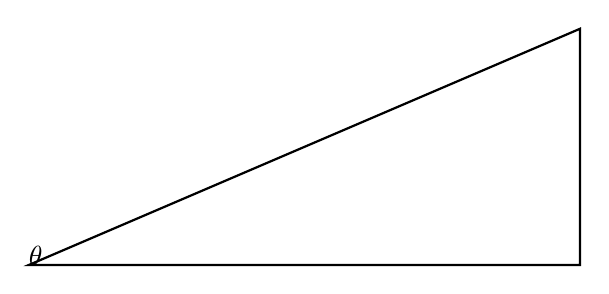
\begin{tikzpicture}[thick]
\coordinate (O) at (0,0);
\coordinate (A) at (7,0);
\coordinate (B) at (7,3);
\draw (O)--(A)--(B)--cycle;

%\tkzLabelSegment[below=2pt](O,A){\textit{adjacent leg}}
%\tkzLabelSegment[left=2pt](O,B){\textit{hypotenuse}}
%\tkzLabelSegment[above right=2pt](A,B){\textit{opposite leg}}

\tkzLabelSegment[below=5pt](O,A){\textit{x}}
\tkzLabelSegment[above left=5pt](O,B){\textit{r}}
\tkzLabelSegment[right=5pt](A,B){\textit{y}}

\tkzMarkAngle[fill= orange,size=1.5cm, opacity=.4](A,O,B)
\tkzLabelAngle[pos = 2](A,O,B){\texttt{$\theta$}}

% \tkzMarkAngle[fill= orange,size=0.65cm, opacity=.4](A,O,B)
% \tkzLabelAngle[pos = 0.35](A,O,B){$\gamma$}
%
% \tkzMarkAngle[fill= orange,size=0.8cm, opacity=.4](B,A,O)
% \tkzLabelAngle[pos = 0.6](B,A,O){$\alpha$}
%
% \tkzMarkAngle[fill= orange,size=0.7cm, opacity=.4](O,B,A)
% \tkzLabelAngle[pos = 0.5](O,B,A){$\beta$}

\end{tikzpicture}

\item Du har nytta av metoderna \code{math.cos(theta)} och \code{math.sin(theta)} vid omvandling från polära koordinater.

\item Attributet \code{negY} kommer att underlätta för dig när du på laborationen ska omvandla en punkt till fönsterkoordinater där y-axeln är omvänd jämfört med kartesiska koordinater.

\item Notera att klassens attribut är av typen \code{Double} och inte \code{Int}, trots att vi senare ska använda punkten för att beskriva en diskret pixelposition. Anledningen till detta är att det kan uppstå avrundningsfel vid numeriska beräkningar. Detta blir särskilt märkbart vid upprepad räkning med små värden, t.ex. när man ritar en approximerad cirkel med många linjesegment.
\end{itemize}

\SOLUTION

\TaskSolved \what~
\begin{Code}
package graphics

case class Point(x: Double, y: Double) {
  val r: Double          = math.hypot(x, y)
  val theta: Double      = math.atan2(y, x)
  def negY: Point        = Point(x, -y)
  def +(p: Point): Point = Point(x + p.x, y + p.y)
}
object Point {
  def polar(r: Double, theta: Double): Point =
    Point(r * math.cos(theta), r * math.sin(theta))
}
\end{Code}

\QUESTEND



\clearpage

\ExtraTasks %%%%%%%%%%%%%%%%%%%%%%%%%%%%%%%%%%%%%%%%%%%%%%%%%%%%%%%%%%%%%%%%%%%%



\WHAT{Instansiering med \code{new} och värdet \code{null}.}

\QUESTBEGIN

\Task  \what~  Man skapar instanser av klasser med \code{new}. Då anropas konstruktorn och plats reserveras i datorns minne för objektet. Variabler av referenstyp som inte refererar till något objekt har värdet \code{null}.

\Subtask Vad händer nedan? Vilka rader ger felmeddelande och i så fall hur lyder felmeddelandet?

\begin{REPL}
scala> class Gurka(val vikt: Int)
scala> var g: Gurka = null
scala> g.vikt
scala> g = new Gurka(42)
scala> g.vikt
scala> g = null
scala> g.vikt
\end{REPL}

\Subtask Rita minnessituationen efter raderna 2, 4, 6.

\SOLUTION


\TaskSolved \what


\SubtaskSolved  Rad 3 och 7 ger båda felmeddelandet \code{java.lang.NullPointerException},  på grund av försök att referera medlemmar med hjälp av en \code{null}-referens, som alltså inte pekar på något objekt.

\SubtaskSolved  \includegraphics[scale=0.6]{../img/w06-solutions/1b}


\QUESTEND


\WHAT{Klasser,  instanser och skräp.}

\QUESTBEGIN

\Task  \what~För länge sedan i en galax långt långt borta...

\begin{Code}
case class Arm(ärTillVänster: Boolean)

case class Ben(ärTillVänster: Boolean)

case class Huvud(harHår: Boolean = true)

case class Rymdvarelse (
      arm1:   Arm   = Arm(true),
      arm2:   Arm   = Arm(false),
      ben1:   Ben   = Ben(true),
      ben2:   Ben   = Ben(false),
      huvud1: Huvud = Huvud(harHår = false),
  var huvud2: Huvud = Huvud()
) {
  def ärSkallig = !huvud1.harHår && !huvud2.harHår
}
\end{Code}

\Subtask Klistra in ovan rymdkod i REPL och evaluera nedan rader. Rita minnessituationen efter rad 5 och beskriv vad som händer.
\begin{REPL}
scala> val alien = Rymdvarelse()
scala> alien.ärSkallig
scala> val predator = Rymdvarelse()
scala> predator.ärSkallig
scala> predator.huvud2 = alien.huvud1
scala> predator.huvud2 eq alien.huvud1  // test av referenslikhet
scala> println(predator)
scala> predator.ärSkallig
\end{REPL}

\Subtask Vad händer så småningom med det ursprungliga \code{huvud2}-objektet i predator efter tilldelningen på rad 5? Går det att referera till detta objekt på något sätt?

\SOLUTION

\TaskSolved \what

\SubtaskSolved  Vi skapar två rymdvarelser, \code{alien} och \code{predator}, med vardera två ben och två armar, samt vardera två huvuden (där det ena är skalligt och det andra har hår). Efter det är varken \code{alien} eller \code{predator} skallig eftersom båda har ett huvud med hår. Sen låter man referensen till \code{predator}s huvud med hår referera till aliens huvud utan hår. Nu är predator helt skallig och delar huvud med alien.

\includegraphics[scale=0.65]{../img/w06-solutions/2b}

\SubtaskSolved  Eftersom det inte längre finns någon referens som pekar på det objektet kommer skräpsamlaren att ta hand om det och det kommer förr eller senare skrivas över av något annat när platsen i minnet behövs. Objekt som inte har någon referens tills sig går inte att komma åt.

\QUESTEND




\WHAT{Case-klass. Oföränderlig kvadrat.}

\QUESTBEGIN

\Task \label{task:Square} \what~

\Subtask Implementera nedan kvadrat med en editor och klistra in den i REPL.

\begin{Code}
case class Square(val x: Int = 0, val y: Int = 0, val side: Int = 1) {
  val area: Int = ???

  /** Creates a new Square moved to position (x + dx, y + dy) */
  def moved(dx: Int, dy: Int): Square = ???

  def isEqualSizeAs(that: Square): Boolean = ???

  /** Multiplies the side with factor and rounded to nearest integer */
  def scale(factor: Double): Square = ???
}
object Square {
  /** A Square at (0, 0) with side 1 */
  val unit: Square = ???
}
\end{Code}

\Subtask Testa din kvadrat enligt nedan. Förklara vad som händer.

\begin{REPL}
scala> val (s1, s2) = (Square(), Square(1, 10, 1))
scala> val s3 = s1 moved (1,-5)
scala> s1 isEqualSizeAs s3
scala> s2 isEqualSizeAs s1
scala> s1 isEqualSizeAs Square.unit
scala> s2.scale(math.Pi) isEqualSizeAs s2
scala> s2.scale(math.Pi) isEqualSizeAs s2.scale(math.Pi)
scala> s2.scale(math.Pi) eq s2.scale(math.Pi)
scala> Square.unit eq Square.unit
\end{REPL}

\SOLUTION

\TaskSolved \what

\SubtaskSolved

\begin{Code}
case class Square(val x: Int = 0, val y: Int = 0, val side: Int = 1) {
	val area: Int = side * side

	def moved(dx: Int, dy: Int): Square = new Square(x + dx, y + dy, side)

	def isEqualSizeAs(that: Square): Boolean = this.side == that.side

	def scale(factor: Double): Square =
    Square(x, y, (side * factor).round.toInt)
}

object Square {
	val unit: Square = Square()
}
\end{Code}

\SubtaskSolved
\begin{REPL}
scala> val (s1, s2) = (Square(), Square(1, 10, 1))
s1: Square = Square(0,0,1)
s2: Square = Square(1,10,1)

scala> val s3 = s1 moved (1,-5)
s3: Square = Square(1,-5,1)

scala> s1 isEqualSizeAs s3       // lika storlek
res55: Boolean = true

scala> s2 isEqualSizeAs s1       // lika storlek
res56: Boolean = true

scala> s1 isEqualSizeAs Square.unit   // s1 har sidan 1
res57: Boolean = true

scala> s2.scale(math.Pi) isEqualSizeAs s2  // olika storlek
res58: Boolean = false

scala> s2.scale(math.Pi) == s2.scale(math.Pi) // lika innehåll
res59: Boolean = true

scala> s2.scale(math.Pi) eq s2.scale(math.Pi)  // olika objekt
res60: Boolean = false

scala> Square.unit eq Square.unit   // samma objekt
res61: Boolean = true
\end{REPL}

\QUESTEND



\WHAT{Förändrinsbar Java-klass.}

\QUESTBEGIN

\Task \what~Översätt nedan Scala-klass till Java-klassen \code{JMutablePoint3D}. Alla attribut ska vara privata (varför?). Översätt defaultargumentet till en alternativ konstruktor. Kalla setters för t.ex. \jcode{setX}. Kör \code{javac} och testa i REPL.

\begin{Code}
class MutablePoint3D(var x: Int, var y: Int, var z: Int = 0)
\end{Code}

\SOLUTION

\TaskSolved \what~

\javainputlisting[numbers=left]{examples/JMutablePoint3D.java}

\begin{REPL}
> atom JMutablePoint3D.java
> javac JMutablePoint3D.java
> ls
JMutablePoint3D.class  JMutablePoint3D.java
> scala
Welcome to Scala 2.12.3 (Java HotSpot(TM) 64-Bit Server VM, Java 1.8.0_121).
Type in expressions for evaluation. Or try :help.

scala> val p = new JMutablePoint3D(1,2)
p: JMutablePoint3D = JMutablePoint3D@2cae9b8

scala> p.x
<console>:13: error: value x is not a member of JPoint3D

scala> p.getZ
res0: Int = 0

scala> p.setZ(3)

scala> p.getZ
res1: Int = 3

\end{REPL}

\QUESTEND






\clearpage

\AdvancedTasks %%%%%%%%%%%%%%%%%%%%%%%%%%%%%%%%%%%%%%%%%%%%%%%%%%%%%%%%%%%%%%%%%


\WHAT{Attributrepresentation. Privat konstruktor. Fabriksmetod.}

\QUESTBEGIN

\Task \what~Kim Kodkunnig skapade för länge sedan denna klass som används på många ställen i befintlig kod:

\begin{Code}
class Point private (val x: Int, val y: Int)
object Point {
  def apply(x: Int = 0, y: Int = 0): Point = new Point(x, y)
  val origo = apply()
}
\end{Code}

\Subtask Vad händer om du försöker instansiera Kim Kodkunnigs klass direkt med nyckelordet \code{new}?

\Subtask Varför använder Kim Kodkunnig ett kompanjonsobjekt med en fabriksmetod? Vilka accessregler gäller mellan ett kompanjonsobjekt och klassen med samma namn?

\Subtask Hjälp Kim Kodkunnig att ändra attributrepresentationen så att det oföränderliga tillståndet utgörs av en 2-tupel \code{val p: (Int, Int)} i stället. Befintlig kod ska inte behöva ändras och klassen \code{Point} ska bete sig från ''utsidan'' precis som innan.

\SOLUTION

\TaskSolved \what~

\SubtaskSolved Det blir kompileringsfel eftersom konstruktorn är privat.
\begin{REPL}
scala> :paste

class Point private (val x: Int, val y: Int)
object Point {
  def apply(x: Int = 0, y: Int = 0): Point = new Point(x, y)
  val origo = apply()
}

scala> new Point(0,0)
<console>:14: error: constructor Point in class Point cannot be accessed
\end{REPL}

\SubtaskSolved
\begin{itemize}
  \item Genom att ha en privat konstruktor och bara göra indirekt instansiering via fabriksmetod är lätt ändra attributrepresentation i framtiden utan att befintlig kod behöver ändras.

  \item Med en \code{apply}-metod i kompansjonsobjektet kan man instansiera genom att skriva \code{Point(1, 2)} utan new.

  \item Accessreglerna för kompanjonsobjekt är sådana att kompanjoner ser varandras privata delar.
\end{itemize}

\SubtaskSolved

\begin{Code}
class Point private (private val p: (Int, Int)) {
  def x: Int = p._1
  def y: Int = p._2
}
object Point {
  def apply(x: Int = 0, y: Int = 0): Point = new Point(x, y)
  val origo = apply()
}
\end{Code}

\QUESTEND



\WHAT{Synlighet av klassparametrar och konstruktor, \code{private[this]}.}

\QUESTBEGIN

\Task  \what~

\Subtask En av gurk-klasserna nedan är trasig. Varför och vad blir det för fel?

\begin{Code}
class Gurka1(vikt: Int)

class Gurka2(val vikt: Int)

class Gurka3(private val vikt: Int)

class Gurka4(private val vikt: Int, kompis: Gurka4){
  def kompisVikt = kompis.vikt
}

class Gurka5(private[this] val vikt: Int, kompis: Gurka5){
  def kompisVikt = kompis.vikt
}

class Gurka6 private (vikt: Int)

class Gurka7 private (var vikt: Int)
object Gurka7 {
  def apply(vikt: Int) = {
    require(vikt >= 0, "negativ vikt: " + vikt)
    new Gurka7(vikt)
  }
}
\end{Code}

\Subtask Undersök nedan vad nyckelorden \code{val} och \code{private} får för konsekvenser. Förklara vad som händer. Vilka rader ger vilka felmeddelanden?

\begin{REPL}
scala> new Gurka1(42).vikt
scala> new Gurka2(42).vikt
scala> new Gurka3(42).vikt
scala> val ingenGurka: Gurka4 = null
scala> new Gurka4(42, ingenGurka).kompisVikt
scala> new Gurka4(42, new Gurka4(84, null)).kompisVikt
scala> new Gurka6(42)
scala> new Gurka7(-42)
scala> Gurka7(-42)
scala> val g = Gurka7(42)
scala> g.vikt
scala> g.vikt = -1
scala> g.vikt
\end{REPL}


\SOLUTION


\TaskSolved \what

\SubtaskSolved \code{Gurka5} är trasig. Eftersom vikten i \code{Gurka5} är privat för instansen och inte klassen kan en instans inte accessa en annan instans vikt.
\begin{REPL}
  error: value vikt is not a member of Gurka5
  def kompisVikt = kompis.vikt
\end{REPL}


\SubtaskSolved
\begin{REPL}
scala> new Gurka1(42).vikt
<console>:13: error: value vikt is not a member of Gurka1
       new Gurka1(42).vikt
                      ^

scala> new Gurka2(42).vikt
res64: Int = 42

scala> new Gurka3(42).vikt
<console>:13: error: value vikt in class Gurka3 cannot be accessed in Gurka3
       new Gurka3(42).vikt
                      ^

scala> val ingenGurka: Gurka4 = null
ingenGurka: Gurka4 = null

scala> new Gurka4(42, ingenGurka).kompisVikt
java.lang.NullPointerException
  at Gurka4.kompisVikt(<console>:13)
  ... 36 elided

scala> new Gurka4(42, new Gurka4(84, null)).kompisVikt
res67: Int = 84

scala> new Gurka6(42)
<console>:13: error: constructor Gurka6 in class Gurka6 cannot be accessed
       new Gurka6(42)
       ^

scala> new Gurka7(-42)
<console>:14: error: constructor Gurka7 in class Gurka7 cannot be accessed
       new Gurka7(-42)
       ^

scala> Gurka7(-42)
java.lang.IllegalArgumentException: requirement failed: negativ vikt: -42


scala> val g = Gurka7(42)
g: Gurka7 = Gurka7@70717ed5

scala> g.vikt
res71: Int = 42

scala> g.vikt = -1
g.vikt: Int = -1

scala> g.vikt
res72: Int = -1
\end{REPL}

\QUESTEND





\WHAT{Egendefinierad setter kombinerat med privat konstruktor.}

\QUESTBEGIN

\Task  \what~Klistra in denna kod i REPL:

\begin{Code}
class Gurka8 private (private var _vikt: Int) {
  def vikt = _vikt
  def vikt_=(v: Int): Unit = {
    require(v >= 0, "negativ vikt: " +v)
    _vikt = v
  }
}

object Gurka8 {
  def apply(vikt: Int) = {
    require(vikt >= 0, "negativ vikt: " + vikt)
    new Gurka8(vikt)
  }
}
\end{Code}


\Subtask Förklara vad som händer nedan. Vilka rader ger vilka felmeddelanden?
\begin{REPL}
scala> val g = Gurka8(-42)
scala> val g = Gurka8(42)
scala> g.vikt
scala> g.vikt = 0
scala> g.vikt = -1
scala> g.vikt += 42
scala> g.vikt -= 1000
\end{REPL}

\Subtask Vad är fördelen med möjligheten att skapa egendefinierade setters?

\SOLUTION


\TaskSolved \what


\SubtaskSolved

Rad 1:
\begin{REPL}
	java.lang.IllegalArgumentException: requirement failed: negativ vikt: -42
\end{REPL}
\code{Gurka8.apply} kräver att \code{vikt >= 0} annars kastar \code{require} ett undantag.

Rad 5:
\begin{REPL}
	java.lang.IllegalArgumentException: requirement failed: negativ vikt: -1
\end{REPL}
Settern \code{vikt_=} kräver att \code{vikt >= 0} annars kastar \code{require} ett undantag.

Rad 7:
\begin{REPL}
	java.lang.IllegalArgumentException: requirement failed: negativ vikt: -958
\end{REPL}
Eftersom \code{42 - 1000} är mindre än noll kastar \code{require} ett undantag.

\SubtaskSolved  Man kan sätta egna mer specifika krav på vad som får göras med värdena så man har större koll på att inget oväntat händer.

\QUESTEND




\WHAT{Objekt med föränderligt tillstånd \Eng{mutable state}.}

\QUESTBEGIN

\Task  \what~  Du ska implementera en modell av en hoppande groda som uppfyller följande krav:
\begin{enumerate}%[nolistsep, noitemsep]
\item Varje grodobjekt ska hålla reda på var den är.
\item Varje grodobjekt ska hålla reda på hur långt grodan hoppat totalt.
\item Varje grodobjekt ska kunna beräkna hur långt det är mellan grodans nuvarande position och utgångsläget.
\item Alla grodor börjar sitt hoppande i origo.
\item En groda kan hoppa enligt två metoder:
  \begin{itemize} [nolistsep, noitemsep]
  \item relativ förflyttning enligt parametrarna \code{dx} och \code{dy},
  \item slumpmässig relativ förflyttning $[1, 10]$ i x-ledsförändring och $[1, 10]$ i y-ledsförändring.
  \end{itemize}
\end{enumerate}

\Subtask Implementera klassen \code{Frog} enligt nedan kodskelett och ovan krav.

\begin{Code}
class Frog private (initX: Int = 0, initY: Int = 0) {
  def x: Int = ???
  def y: Int = ???

  def jump(dx: Int, dy: Int): Unit = ???
  def randomJump: Unit = ???

  def distanceToStart: Double = ???
  def distanceJumped: Double = ???
  def distanceTo(that: Frog): Double = ???
}
object Frog {
  def spawn(): Frog = ???
}
\end{Code}
\emph{Tips:}
\begin{itemize} [nolistsep, noitemsep]
\item Om namnet man vill ge ett privat föränderligt attribut ''krockar'' med ett metodnamn, är det vanligt att man börjar attributets namn med understreck, t.ex. \code{private var _x } för att på så sätt undkomma namnkonflikten.
\item Inför en metod i taget och klistra in den nya grodan i REPL efter varje utvidgning och testa.
\end{itemize}



\Subtask Skapa en metod \code{def test(): Unit} i ett singelobjekt \code{FrogTest} som innehåller kod som gör minst en kontroll av varje krav. Om ingen kontroll går fel ska \code{"Test Ok!"} skrivas ut annars ska exekveringen avbrytas. \emph{Tips:} Använd \code{assert(b, msg)} som avbryter exekveringen och skriver ut \code{msg} om \code{b} är falsk.

\Subtask Vad kallas en metod som enbart returnerar värdet av ett privat attribut?

\Subtask Inför setters för attributen som håller reda på x- och y-postitionen. Förändringar av positionen i x- eller y-led ska räknas som ett hopp och alltså registreras i det attribut som håller reda på det ackumulerade hoppavståndet.

\Subtask Simulera ett massivt grodhoppande med krockdetektering genom att skapa 100 grodor som till att börja med är placerade på x-axeln med avståndet $8$ längdenheter mellan sig. För varje runda i en \code{while}-sats, låt en slumpässigt vald groda göra ett \code{randomJump} tills någon groda befinner sig närmare än $0.5$ längdenheter, vilket är definitionen på att de har krockat. Räkna hur många looprundor som behövs innan något grodpar krockar och skriv ut antalet. Skriv även ut det totala antalet \\ \emph{Tips:} Börja med pseudokod på papper. Använd en grodvektor.


\SOLUTION


\TaskSolved \what


\SubtaskSolved
\begin{Code}
class Frog private (initX: Int = 0, initY: Int = 0) {
	private var _x: Int = initX
	private var _y: Int = initY
	private var _distanceJumped: Double = 0

  def x: Int = _x
  def y: Int = _y

	def jump(dx: Int, dy: Int): Unit = {
		_x += dx
		_y += dy
		_distanceJumped += math.hypot(dx, dy)
	}


	def randomJump: Unit = {
		def rnd = util.Random.nextInt(10) + 1
		jump(rnd, rnd)
	}

	def distanceToStart: Double = math.hypot(x,y)
	def distanceJumped: Double = _distanceJumped
	def distanceTo(f: Frog): Double = math.hypot(x - f.x, y - f.y)
}

object Frog {
	def spawn(): Frog = new Frog()
}
\end{Code}

\SubtaskSolved Exempel på testprogram:
\begin{Code}
object FrogTest {
  def test(): Unit = {
    val f1 = Frog.spawn()
    assert(f1.x == 0 && f1.y == 0, "Test of spawn, reqt 1 & 4 failed.")

    f1.jump(4,3)
    assert(f1.x == 4 && f1.y == 3, "Test of jump, reqt 1 & 4 failed.")

    f1.jump(4,3)
    assert(f1.distanceJumped == 10, "Test of jump, reqt 2 failed.")

    f1.jump(-4,-3)
    assert(f1.distanceToStart == 5, "Test of jump, reqt 3 failed.")

    for (x <- 1 to 10000) {
      val f2 = Frog.spawn()
    	f2.randomJump
    	assert(f2.x > 0 && f2.x <= 10 && f2.y > 0 && f2.y <= 10,
            "Test of randomJump, reqt 5 failed.")
    }
    println("Test Ok!")
  }
}
\end{Code}

\SubtaskSolved  En metod som är en indirekt avläsning av attrubtvärden kallas getter.

\SubtaskSolved
\begin{Code}

class Frog private (initX: Int = 0, initY: Int = 0) {
	private var _x: Int = initX
	private var _y: Int = initY
	private var _distanceJumped: Double = 0

	def jump(dx: Int, dy: Int): Unit = {
		_x += dx
		_y += dy
		_distanceJumped += math.hypot(dx, dy)
	}

	def x: Int = _x
  def x_= (newX: Int): Unit = { // Setter för x
		_distanceJumped += math.abs(x - newX)
		_x = newX
	}

  def y: Int = _y
	def y_= (newY: Int): Unit = { // Setter för y
		_distanceJumped += math.abs(y - newY)
		_y = newY
	}


	def randomJump: Unit = {
		def rnd = util.Random.nextInt(10) + 1
		jump(rnd, rnd)
	}

	def distanceToStart: Double = math.hypot(x,y)
	def distanceJumped: Double = _distanceJumped
	def distanceTo(f: Frog): Double = math.hypot(x - f.x, y - f.y)
}

object Frog {
	def spawn(): Frog = new Frog()
}

\end{Code}

\SubtaskSolved
\begin{Code}
object frogSimulation {
  def isAnyCollision(frogs: Vector[Frog]): Boolean = {
    var found = false
    frogs.indices.foreach { i =>  // generate all pairs (i,j)
      for (j <- i + 1 until frogs.size)
        if (!found) found = frogs(i).distanceTo(frogs(j)) <= 0.5
    }
    found
  }

  def jumpUntilCrash(n: Int = 100, initDist: Int = 8): (Int, Double) = {
    val frogs = Vector.fill(n)(Frog.spawn)
    (0 until n).foreach(i => frogs(i).x = i * initDistance)
    var count = 0
    while (!isAnyCollision(frogs)) {
      frogs(util.Random.nextInt(n)).randomJump
    	count += 1
    }
    (count, frogs.map(_.distanceJumped).sum)
  }

  def run(nbrOfCrashTests: Int = 10) = for (i <- 1 to nbrOfCrashTests) {
    val (n, dist) = jumpUntilCrash()
    println(s"\nAntalet looprundor innan grodkrock: $n")
    println(s"Totalt avstånd hoppat av alla grodor: $dist")
  }
}
\end{Code}

\QUESTEND




\QUESTBEGIN

\Task  \what~  Webbshoppen \textbf{UberSquare} säljer flyttbara kvadrater. I affärsmodellen ingår att ta betalt per förflyttning. Du ska hjälpa UberSquare att utveckla en enkel prototyp för att imponera på riskkapitalister.

\Subtask Implementera \code{Square} enligt dokumentationskommentarerna i efterföljande kodskiss och enligt dessa krav:

\begin{enumerate}%[nolistsep, noitemsep]
   \item Varje instans av \code{Square} ska räkna antalet förflyttningar som gjorts sedan instansen konstruerats.

   \item För att kunna övervaka sina kunder vill UberSquare även räkna det totala antalet förflyttningar som gjorts av alla kvadrater som någonsin skapats (s.k. \emph{big data}).

  \item Varje gång förflyttning sker ska ett visst belopp adderas till den ackumulerade kostnaden för respektive kvadrat, enligt kostnadsberäkningen i krav 4.

  \item UberSquare är oroliga för att kvadraterna flyttas för långt bort och bestämmer därför att för varje förflyttning ska den ackumulerade kvadratkostnaden ökas med den nya positionens avstånd till ursprungsläget vid kvadratens konstruktion multiplicerat med aktuell storlek på kvadraten.

  \item För att framstå som goda berättar UberSquare i sin marknadsföring att skala är gratis att använda. \footnote{D.v.s ett anrop av metoden \code{scale} orsakar ingen omedelbar kostnad.}
\end{enumerate}

\begin{CodeSmall}
/** A mutable and expensive Square. */
class Square private (val initX: Int, val initY: Int, val initSide: Int) {
  private var nMoves = 0;
  private var sumCost = 0.0;

  private var _x = initX;
  private var _y = initY;

  private var _side = initSide;

  private def addCost(): Unit = {
   sumCost += ???
  }

  def x: Int = ???
  def y: Int = ???

  def side = ???

  /** Scales the side of this square and rounds it to nearest integer */
  def scale(factor: Double): Unit = ???

  /** Moves this square to position (x + xd, y + dy) */
  def move(dx: Int, dy: Int): Unit = ???

  /** Moves this square to position (x, y) */
  def moveTo(x: Int, y: Int): Unit = ???

  /** The accumulated cost of this Square */
  def cost: Double = ???

  /** Returns the accumulated cost. Sets the accumulated cost to zero. */
  def pay: Double = ???

  override def toString: String =
    s"Square[($x, $y), side: $side, #moves: $nMoves times, cost: $sumCost]"
}


object Square {
  private var created = Vector[Square]()

  /** Constructs a new Square object at (x, y) with size side */
  def apply(x: Int, y: Int, side: Int): Square = {
    require(side >= 0, s"side must be positive: $side")
    ???
  }

  /** Constructs a new Square object at (0, 0) with side 1 */
  def apply(): Square = ???

  /** The total number of moves that have been made for all squares. */
  def totalNumberOfMoves: Int = ???

  /** The total cost of all squares. */
  def totalCost: Double = ???
}
\end{CodeSmall}

\Subtask Testa din kvadratprototyp i REPL. Använd t.ex. koden nedan:
\begin{REPL}
scala> val xs = Vector.fill(10)(Square())
scala> xs.foreach(_.move(2, 3))
scala> xs.foreach(_.scale(2.9))
scala> val (m, c) = (Square.totalNumberOfMoves, Square.totalCost)
m: Int = 10
c: Double = 36.055512754639885
\end{REPL}

\SOLUTION

\TaskSolved \what~

\begin{CodeSmall}
class Square private (val initX: Int, val initY: Int, val initSide: Int) {
  private var nMoves = 0;
  private var sumCost = 0.0;

  private var _x = initX;
  private var _y = initY;

  private var _side = initSide;

  private def addCost(): Unit = {
   sumCost += math.hypot(x - initX, y - initY) * side
  }

  def x: Int = _x
  def y: Int = _y

  def side = _side

  def scale(factor: Double): Unit = { _side = (_side * factor).round.toInt }

  def move(dx: Int, dy: Int): Unit = {
    _x += dx; _y += dy;
    nMoves += 1
    addCost()
  }

  def moveTo(x: Int, y: Int): Unit = {
    _x = x; _y = y;
    nMoves += 1
    addCost()
  }

  def cost: Double = sumCost

  def pay: Double = {val temp = sumCost; sumCost = 0; temp}

  override def toString: String =
    s"Square[($x, $y), side: $side, #moves: $nMoves times, cost: $sumCost]"
}
object Square {
  private var created = Vector[Square]()

  def apply(x: Int, y: Int, side: Int): Square = {
    require(side >= 0, s"side must be positive: $side")
    val sq = (new Square(x, y, side))
    created :+= sq
    sq
  }

  def apply(): Square = apply(0, 0, 1)

  def totalNumberOfMoves: Int = created.map(_.nMoves).sum

  def totalCost: Double = created.map(_.cost).sum
}
\end{CodeSmall}

\QUESTEND



\WHAT{Hjälpkonstruktor.}

\QUESTBEGIN

\Task\Uberkurs \label{task:aux-constructor} \what~I tidigare uppgifter har vi möjliggjort alternativa sätt att skapa instanser genom default-argument och fabriksmetoder i kompanjonsobjekt.

Ett annat sätt att göras detta på, som i Scala är ovanligt\footnote{Men i Java är detta mycket vanligt då defaultargument m.m. inte ingår i språket.}, är att definiera flera konstruktorer inne i klasskroppen. I Scala kallas en sådan extra konstruktor för \textbf{hjälpkonstruktor} \Eng{auxiliary constructor}.

En hjälpkonstruktor skapar man i Scala genom att definiera en metod som har det speciella namnet \code{this}, alltså en deklaration \code{def this(...) = ...} Hjälpkonstruktorer måste börja med att anropa en annan konstruktor, antingen den primära konstruktorn (d.v.s. den som klasshuvudet definierar) eller en tidigare definierad  hjälpkonstruktor.

\Subtask Läs mer om hjälpkonstruktorer här: \\ \href{http://www.artima.com/pins1ed/functional-objects.html#6.7}{www.artima.com/pins1ed/functional-objects.html\#6.7}

\Subtask Hitta på en egen uppgift med hjälpkonstruktorer, baserat på någon av klasserna i tidigare övningar.


%\Task \TODO \\ \code{class Rational private (numerator: BigInt, denominator: BigInt)} \\
%Inspirerat av Rational i pins1ed med GCD\SOLUTION

\QUESTEND


%!TEX encoding = UTF-8 Unicode
%!TEX root = ../exercises.tex

\ifPreSolution



\Exercise{\ExeWeekSIX}\label{exe:W06}

\begin{Goals}
\item Kunna skapa och använda \code{match}-uttryck med konstanta värden, garder och mönstermatchning med case-klasser.
\item Kunna skapa och använda case-objekt för matchningar på uppräknade värden.
\item Kunna hantera saknade värden med hjälp av typen \code{Option} och mönstermatchning på \code{Some} och \code{None}.
\item Kunna fånga undantag med \code{scala.util.Try}.
\item Känna till \code{try}, \code{catch} och \code{throw}.
%\item Känna till \jcode{switch}-satser i Java.
\item Känna till nyckelordet \code{sealed} och förstå nyttan med förseglade typer.
%\item Känna till relationen mellan \code{hashCode} och \code{equals}.
%\item Kunna skapa partiella funktioner med case-uttryck.
%\item Känna till betydelsen av små och stora begynnelsebokstäver i case-grenar i en matchning, samt förstå hur namn binds till värden in en case-gren.
%\item Kunna använda \code{flatMap} tillsammans med \code{Option} och \code{Try}.
%\item Känna till skillnaderna mellan \code{try}-\code{catch} i Scala och java.
\item Känna till att metoden \code{unapply} används vid mönstermatchning.
%\item Kunna implementera \code{equals} med hjälp av en \code{match}-sats, som fungerar för finala klasser utan arv.
%\item Känna till \code{null}.
\end{Goals}

\begin{Preparations}
\item \StudyTheory{06}
\end{Preparations}

\BasicTasks %%%%%%%%%%%%%%%%

\else



\ExerciseSolution{\ExeWeekSIX}

\BasicTasks %%%%%%%%%%%

\fi





% \WHAT{Hur fungerar en \jcode{switch}-sats i Java (och flera andra språk)?}

% \QUESTBEGIN

% \Task \label{task:switch} \what~   Det händer ofta att man vill testa om ett värde är ett av många olika alternativ. Då kan man använda en sekvens av många \code{if}-\code{else}, ett för varje alternativ. Men det finns ett annat sätt i Java och många andra språk: man kan använda \jcode{switch} som kollar flera alternativ i en och samma sats, se t.ex. \href{https://en.wikipedia.org/wiki/Switch_statement}{en.wikipedia.org/wiki/Switch\_statement}.

% \Subtask Skriv in nedan kod i en kodeditor. Spara med namnet \texttt{Switch.java} och kompilera filen med kommandot \texttt{javac Switch.java}. Kör den med \texttt{java Switch} och ange din favoritgrönsak som argument till programmet. Vad händer? Förklara hur \jcode{switch}-satsen fungerar.

% \javainputlisting[numbers=left,basicstyle=\ttfamily\fontsize{9}{11}\selectfont]{examples/Switch.java}

% \Subtask \label{subtask:break} Vad händer om du tar bort \jcode{break}-satsen på rad 16?




% \SOLUTION


% \TaskSolved \what


% \SubtaskSolved  Beroende på första bokstaven i din favoritgrönsak får du olika svar såsom \textit{gurka är gott!} vid första bokstaven $g$.\\
% Javas \jcode{switch}-sats testar den första bokstaven på favoritgrönsaken genom att stegvis jämföra den med \jcode{case}-uttrycken. Om första bokstaven \jcode{firstChar} matchar bokstaven efter ett \jcode{case} körs koden efter kolonet till \jcode{switch}-satsens slut eller tills ett \jcode{break} avbryter \jcode{switch}-satsen.\\
% Matchar inte \jcode{firstChar} något \jcode{case} så finns även \jcode{default}, som körs oavsett vilken första bokstaven är, ett generellt fall.

% \SubtaskSolved  Om \jcode{case 't'} körs kommer både  \textit{tomat är gott!} och \textit{broccoli är gott!} skrivas ut, man säger att koden $"$faller igenom$"$. Utan \jcode{break}-satsen i Java körs koden i efterkommande \jcode{case} tills ett \jcode{break} avbryter exekveringen eller \jcode{switch}-satsen tar slut.



% \QUESTEND






\WHAT{Matcha på konstanta värden.}

\QUESTBEGIN

\Task \label{task:vegomatch} \what~   % I Scala finns ingen \jcode{switch}-sats. I stället har Scala ett \code{match}-uttryck som är mer kraftfullt. Dock saknar Scala nyckelordet \jcode{break} och Scalas \code{match}-uttryck kan inte ''falla igenom'' som skedde i uppgift \ref{task:switch}\ref{subtask:break}.

\Subtask \label{subtask:vegomatch} Skriv nedan program med en kodeditor och spara i filen \texttt{Match.scala}. Kompilera med \texttt{scalac Match.scala}. Kör med \texttt{scala Match} och ge som argument din favoritgrönsak. Vad händer? Förklara hur ett \code{match}-uttryck fungerar.

\scalainputlisting[numbers=left,basicstyle=\ttfamily\fontsize{11}{12}\selectfont]{examples/Match.scala}

\Subtask Vad blir det för felmeddelande om du tar bort case-grenen för defaultvärden och indata väljs så att inga case-grenar matchar? Är det ett exekveringsfel eller ett kompileringsfel?

% \Subtask Beskriv några skillnader i syntax och semantik mellan Javas flervalssats \jcode{switch} och Scalas flervalsuttryck \code{match}.



\SOLUTION


\TaskSolved \what


\SubtaskSolved  Svaret blir identiskt mot föregående uppgiften i Java.\\
Scalas \code{match}-uttryck fungerar väldigt likt Javas \jcode{switch}. Den jämför stegvis värdet med varje \code{case} för att sedan returnera ett värde tillhörande motsvarande \code{case}.

\SubtaskSolved  \begin{REPL}
scala.MatchError (of class java.lang.Character)
\end{REPL}
Exekveringsfel, uppstår av en viss input under körningen.

% \SubtaskSolved  Scalas \code{match} ersätter kolonet (:) i \jcode{switch} med Scalas högerpil (=>).\\
% \code{match} returnerar ett värde till skillnad från \jcode{switch} som inte returnerar något.\\
% \code{match} kan inte $"$falla igenom$"$ så ett \jcode{break} efter varje \jcode{case} är inte nödvändigt.\\
% Till skillnad från \jcode{switch}-satsen kastar \code{match} ett \code{MatchError} om ingen matchning skulle ske.



\QUESTEND






\WHAT{Gard i case-grenar.}

\QUESTBEGIN

\Task  \what~  Med hjälp en gard \Eng{guard} i en case-gren kan man begränsa med ett villkor om grenen ska väljas.

Utgå från koden i uppgift \ref{task:vegomatch}\ref{subtask:vegomatch} och byt ut case-grenen för \code{'g'}-matchning till nedan variant med en gard med nyckelordet \code{if} (notera att det inte behövs parenteser runt villkoret):
\begin{Code}
    case 'g' if math.random() > 0.5 => "gurka är gott ibland..."
\end{Code}
Kompilera om och kör programmet upprepade gånger med olika indata tills alla grenar i \code{match}-uttrycket har exekverats. Förklara vad som händer.

\SOLUTION


\TaskSolved \what

Garden som införts vid \code{case 'g'} slumpar fram ett tal mellan 0 och 1 och om talet inte är större än $0.5$ så blir det ingen matchning med \code{case 'g'} och programmet testar vidare tills default-caset.\\
Gardens krav måste uppfyllas för att det ska matcha som vanligt.



\QUESTEND






\WHAT{Mönstermatcha på attributen i case-klasser.}

\QUESTBEGIN

\Task \label{task:match-caseclass} \what~   Scalas \code{match}-uttryck är extra kraftfulla om de används tillsammans med \code{case}-klasser: då kan attribut extraheras automatiskt och bindas till lokala variabler direkt i case-grenen som nedan exempel visar (notera att \code{v} och \code{rutten} inte behöver deklareras explicit). Detta kallas för \textbf{mönstermatchning}.

\Subtask \label{subtask:autobinding-match} Vad skrivs ut nedan? Varför? Prova att byta namn på \code{v} och \code{rutten}.
\begin{REPL}
scala> case class Gurka(vikt: Int, ärRutten: Boolean)
scala> val g = Gurka(100, true)
scala> g match { case Gurka(v,rutten) => println("G" + v + rutten) }
\end{REPL}

%\TODO Tab två gånger fungerar inte i scala3-repl
\Subtask Skriv sedan nedan i REPL och tryck TAB två gånger efter punkten. Vad har \code{unapply}-metoden för resultattyp?
\begin{REPL}
scala> Gurka.unapply   // Tryck TAB två gånger
\end{REPL}
\begin{Background}
Case-klasser får av kompilatorn automatiskt ett kompanjonsobjekt \Eng{companion object}, i detta fallet \code{object Gurka}. Det objektet får av kompilatorn automatiskt en \code{unapply}-metod. Det är \code{unapply} som anropas ''under huven'' när case-klassernas attribut extraheras vid mönstermatchning, men detta sker alltså automatiskt och man behöver inte explicit nyttja \code{unapply} om man inte själv vill implementera s.k. extraherare \Eng{extractors}; om du är nyfiken på detta, se fördjupningsuppgift \ref{task:extractor}.
\end{Background}

\Subtask Anropa \code{unapply}-metoden enligt nedan. Vad blir resultatet?
\begin{REPL}
scala> Gurka.unapply(g)
\end{REPL}
Vi ska i senare uppgifter undersöka hur typerna \code{Option} och \code{Some} fungerar och hur man kan ha nytta av dessa i andra sammanhang.

% \Subtask Spara programmet nedan i filen \texttt{vegomatch.scala} och kompilera och kör med \code{scala vegomatch.Main 1000} i terminalen. Förklara hur predikatet \code{ärÄtvärd} fungerar.
% \scalainputlisting[numbers=left,basicstyle=\ttfamily\fontsize{11}{12}\selectfont]{examples/vegomatch.scala}
%

\SOLUTION


\TaskSolved \what


\SubtaskSolved  G100true. Vid byte av plats: Gtrue100.\\
\code{match} testar om kompanjonsobjektet \code{Gurka} är av typen \code{Gurka} med två parametervärden. De angivna parametrarna tilldelas namn, \code{vikt} får namnet \code{v} och \code{ärRutten} namnet \code{rutten} och skrivs sedan ut. Byts namnen dessa ges skrivs de ut i den omvända ordningen.

\SubtaskSolved  \code{Option[(Int, Boolean)]}
%TODO detta är inte längre fallet i scala3-repl

%\SubtaskSolved  \code{Some((100, true))}, en \code{Option} med en tupel av parametrarna från g.
\SubtaskSolved	\code{Gurka(100, true)}
%TODO eventuellt skriv mer utförligt

% \SubtaskSolved  \code{ärÄtvärd} testar om \code{Grönsak g} är av typen \code{Gurka(v, rutten)} eller \code{Tomat}. Dessa har sedan garder.\\ \code{Gurka} måste ha \code{vikt} över 100 och \code{ärRutten} vara \code{false} för att \code{case Gurka} ska returnera \code{true}.\\
% \code{Tomat} måste ha \code{vikt} över 50 och \code{ärRutten} vara \code{false} för att \code{case Tomat} ska returnera \code{true}.\\
% Matchas inte \code{Grönsak g} med någon av dessa returneras default-värdet \code{false}.



\QUESTEND







\WHAT{Matcha på case-objekt och nyttan med \code{sealed}.}

\QUESTBEGIN

\Task	\what~	Skriv nedan kodrader i en REPL en för en. Notera nyckelordet \code{sealed} som används för att försegla en typ. En \textbf{förseglad typ} måste ha alla sina subtyper i en och samma kodfil.
\begin{REPL}
scala> sealed trait Färg
scala> case object Spader extends Färg
\end{REPL}
\Subtask Hur lyder felmeddelandet och varför sker det? Är det ett kompileringsfel eller ett körtidsfel?

\Subtask  %\label{task:match-sealedtrait-caseobject}
Skapa nu nedan kod i en editor och klistra in i REPL.
\begin{Code}
object Kortlek:
  sealed trait Färg
  object Färg:
      val values = Vector(Spader, Hjärter, Ruter, Klöver)
  case object Spader extends Färg
  case object Hjärter extends Färg
  case object Ruter extends Färg
  case object Klöver extends Färg
\end{Code}

\Subtask \label{subtask:match-sealedtrait} Skapa en funktion \code{def parafärg(f: Färg): Färg} i en editor, som med hjälp av ett match-uttryck returnerar parallellfärgen till en färg. Parallellfärgen till \code{Hjärter} är \code{Ruter} och vice versa, medan parallellfärgen till \code{Klöver} är \code{Spader} och vice versa. Klistra in funktionen i REPL. Passa även på att skriva en \code{import-sats} för det yttre objektet \textbf{Kortlek}, så medlemmarna av objektet kan nås enkelt.
\begin{REPL}
scala> parafärg(Spader)
scala> val xs = Vector.fill(5)(Färg.values((math.random() * 4).toInt))
scala> xs.map(parafärg)
\end{REPL}

\Subtask Vi ska nu undersöka vad som händer om man glömmer en av case-grenarna i matchningen i \code{parafärg}. ''Glöm'' alltså avsiktligt en av case-grenarna och klistra in den nya \code{parafärg} med den ofullständiga matchningen. Hur lyder varningen? Kommer varningen vid körtid eller vid kompilering?

\Subtask Anropa \code{parafärg} med den ''glömda'' färgen. Hur lyder felmeddelandet? Är det ett kompileringsfel eller ett körtidsfel?

\Subtask Förklara vad nyckelordet \code{sealed} innebär och vilken nytta man kan ha av att \textbf{försegla} en supertyp.


\SOLUTION


\TaskSolved \what

\SubtaskSolved
%Illegal inheritance from sealed trait Färg
\begin{REPL}
Cannot extend sealed trait Färg in a different source file
\end{REPL}
Felmeddelandet fås av att REPL:en behandlar varje inmatning individuellt och tillåter därför inte att subtypen \code{Spader} förlänger \Eng{extends} supertypen \code{Färg} eftersom denna var förseglad \Eng{sealed}. Mer om detta senare i kursen...

\SubtaskSolved
-

\SubtaskSolved
\begin{Code}
def parafärg(f: Färg): Färg = f match
  case Spader  => Klöver
  case Hjärter => Ruter
  case Ruter   => Hjärter
  case Klöver  => Spader
\end{Code}

\SubtaskSolved
\begin{REPL}
<console>:17: warning: match may not be exhaustive.
It would fail on the following input: Ruter
\end{REPL}
Varningen kommer redan vid kompilering.

\SubtaskSolved
\begin{REPL}
scala.MatchError: Ruter (of class Ruter)
  at .parafärg(<console>:17)
\end{REPL}
Detta är ett körtidsfel.

\SubtaskSolved  Om en klass är \code{sealed} innebär det att om ett element ska matchas och är en subtyp av denna klass så ger Scala varning redan vid kompilering om det finns en risk för ett \code{MatchError}, alltså om \code{match}-uttrycket inte är uttömmande och det finns fall som inte täcks av ett \code{case}.\\
En förseglad supertyp innebär att programmeraren redan vid kompileringstid får en varning om ett fall inte täcks och i sånt fall vilket av undertyperna, liksom annan hjälp av kompilatorn. Detta kräver dock att alla subtyperna delar samma fil som den förseglade klassen.



\QUESTEND


%\WHAT{Mönstermatcha med nyttan av \code{enum}.}

%\QUESTBEGIN

%\Task	\what~ Vi ska nu undersöka och jämföra skillnad mellan nyckelorden \code{enum} och \code{sealed}. Skriv nedan kod i en REPL.
%\begin{Code}
%enum Färg:
%  case Spader, Hjärter, Ruter, Klöver
%\end{Code}

%\Subtask Skapa igen i en editor en funktion \code{def paraFärg(f: Färg): Färg}, nästintill likadan som den som vi skapade i deluppgift \ref{task:match-sealedtrait-caseobject} %\ref{subtask:match-sealedtrait}. Funktionen ska återigen utnyttja match-uttryck för att returnera paralellfärgen till argumentet som ges. Klistra in funktionen i REPL.
%\begin{REPL}
%scala> parafärg(Färg.Ruter)
%scala> val xs = Vector.fill(5)(Färg.values((math.random() * 4).toInt))
%scala> xs.map(parafärg)
%\end{REPL}


%\SOLUTION


%\TaskSolved \what

%\SubtaskSolved
%\begin{Code}
%def parafärg(f: Färg): Färg = f match
%  case Färg.Spader  => Färg.Klöver
%  case Färg.Hjärter => Färg.Ruter
%  case Färg.Ruter   => Färg.Hjärter
%  case Färg.Klöver  => Färg.Spader
%\end{Code}


%\QUESTEND


\WHAT{Betydelsen av små och stora begynnelsebokstäver vid matchning.}

\QUESTBEGIN

\Task  \what~  För att åstadkomma att namn kan bindas till variabler vid matchning utan att de behöver deklareras i förväg (som vi såg i uppgift \ref{task:match-caseclass}\ref{subtask:autobinding-match}) så har identifierare med liten begynnelsebokstav fått speciell betydelse: den tolkas av kompilatorn som att du vill att en variabel  binds till ett värde vid matchningen. En identifierare med stor begynnelsebokstav tolkas däremot som ett konstant värde (t.ex. ett case-objekt eller ett case-klass-mönster).

\Subtask \emph{En case-gren som fångar allt}. En case-gren med en identifierare med liten begynnelsebokstav som saknar gard kommer att matcha allt. Prova nedan i REPL, men försök lista ut i förväg vad som kommer att hända. Vad händer?
\begin{REPL}
scala> val x = "urka"
scala> x match
         case str if str.startsWith("g") => println("kanske gurka")
         case vadsomhelst => println("ej gurka: " + vadsomhelst)
scala> val g = "gurka"
scala> g match
         case str if str.startsWith("g") => println("kanske gurka")
         case vadsomhelst => println("ej gurka: " + vadsomhelst)
\end{REPL}

\Subtask \emph{Fallgrop med små begynnelsbokstäver.} Innan du provar nedan i REPL, försök gissa vad som kommer att hända. Vad händer? Hur lyder varningarna och vad innebär de?
\begin{REPL}
scala> val any: Any = "varken tomat eller gurka"
scala> case object Gurka
scala> case object tomat
scala> any match
         case Gurka => println("gurka")
         case tomat => println("tomat")
         case _ => println("allt annat")
\end{REPL}

\Subtask \emph{Använd backticks för att tvinga fram match på konstant värde.} Det finns en utväg om man inte vill att kompilatorn ska skapa en ny lokal variabel: använd specialtecknet \emph{backtick}, som skrivs \`{} och kräver speciella tangentbordstryck.\footnote{Fråga någon om du inte hittar hur man gör backtick \`{} på ditt tangentbord.}  Gör om föregående uppgift men omgärda nu identifieraren \code{tomat} i tomat-case-grenen med backticks, så här: \code{  case `tomat` => ...}



\SOLUTION


\TaskSolved \what


\SubtaskSolved  Både \code{str} och \code{vadsomhelst} matchar med inputen, oavsett vad denna är på grund av att de har en liten begynnelsebokstav.\\
 \code{str} har dock en gard att strängen måste börja med $g$ vilket gör så endast \code{val g = "gurka"} matchar med denna. \code{val x = "urka"} plockas dock upp av \code{vadsomhelst} som är utan gard.

\SubtaskSolved
\begin{REPL}
<console>:16: warning: patterns after a variable pattern cannot match (SLS 8.1
.1)
\end{REPL}
och
\begin{REPL}
<console>:17: warning: unreachable code due to variable patter 'tomat' on line
16
\end{REPL}
Trots att en klass \code{tomat} existerar så tolkar Scalas \code{match} den som en \code{case}-gren som fångar allt på grund av en liten begynnelsebokstav. Detta gör så alla objekt som inte är av typen \code{Gurka} kommer ge utskriften \textit{tomat} och att sista caset inte kan nås.

\SubtaskSolved
\begin{Code}
case `tomat` => println("tomat")
\end{Code}



\QUESTEND





\WHAT{Matcha på innehåll i en Vector.}

\QUESTBEGIN

\Task \what ~ Kör nedan i REPL. Vad skrivs ut? Förklara vad som händer.
\begin{REPL}
scala> val xss = Vector(Vector("hej"),Vector("på", "dej"),Vector("4","x","2"))
scala> xss.map( _ match
  case Vector() => "tom"
  case Vector(a) => a.reverse
  case Vector(_, b) => b.reverse
  case Seq(a, "x", b) => a + b
  case _ => "ANNARS DETTA"
  ).foreach(println)
\end{REPL}


\SOLUTION

\TaskSolved \what

\begin{REPL}
jeh
jed
42
\end{REPL}
För varje element i \code{xss} görs en matching som resulterar i en sträng. Vad som händer i varje gren förklaras nedan.
\begin{enumerate}
  \item Första match-grenen aktiveras aldrig eftersom \code{xss} ej innehåller någon tom vektor.
  \item Andra grenen passar med \code{Vector("hej")} och variablen \code{a} binds till \code{"hej"}.
  \item Tredje grenen matchar \code{Vector("på", "dej")} där första värdet binds inte till någon variabel eftersom understreck finns på motsvarande plats, medan andra värdet binds till \code{b}.
  \item Fjärde grenen matchar en sekvens med tre värden där mittenvärdet är \code{"x"}. Den sista grenen aktiveras inte i detta exempel men hade matchat allt som inte fångas av tidigare grenar.
\end{enumerate}

\QUESTEND




\WHAT{Använda \code{Option} och matcha på värden som kanske saknas.}

\QUESTBEGIN

\Task  \what~  Man behöver ofta skriva kod för att hantera värden som eventuellt saknas, t.ex. saknade telefonnummer i en persondatabas. Denna situation är så pass vanlig att många språk har speciellt stöd för saknande värden.

I Java\footnote{Scala har också \code{null} men det behövs bara vid samverkan med Java-kod.} används värdet \code{null} för att indikera att en referens saknar värde. Man får då komma ihåg att testa om värdet saknas varje gång sådana värden ska behandlas, t.ex. med \code+if (ref != null) { ...} else { ... }+. Ett annat vanligt trick är att låta \code{-1} indikera saknade positiva heltal, till exempel saknade index, som får behandlas med \code+if (i != -1) { ...} else { ... }+.

I Scala finns en speciell typ \code{Option} som möjliggör smidig och typsäker hantering av saknade värden. Om ett kanske saknat värde packas in i en \code{Option} \Eng{wrapped in an Option}, finns det i en speciell slags samling som bara kan innehålla \emph{inget} eller \emph{något} värde, och alltså har antingen storleken \code{0} eller \code{1}.

\Subtask Förklara vad som händer nedan.
\begin{REPL}
scala> var kanske: Option[Int] = None
scala> kanske.size
scala> kanske = Some(42)
scala> kanske.size
scala> kanske.isEmpty
scala> kanske.isDefined
scala> def ökaOmFinns(opt: Option[Int]): Option[Int] = opt match
         case Some(i) => Some(i + 1)
         case None    => None
scala> val annanKanske = ökaOmFinns(kanske)
scala> def öka(i: Int) = i + 1
scala> val merKanske = kanske.map(öka)
\end{REPL}

\Subtask Mönstermatchingen ovan är minst lika knölig som en \code{if}-sats, men tack vare att en \code{Option} är en slags (liten) samling finns det smidigare sätt. Förklara vad som händer nedan.
\begin{REPL}
val meningen = Some(42)
val ejMeningen = Option.empty[Int]
meningen.map(_ + 1)
ejMeningen.map(_ + 1)
ejMeningen.map(_ + 1).orElse(Some("saknas")).foreach(println)
meningen.map(_ + 1).orElse(Some("saknas")).foreach(println)
\end{REPL}

\Subtask \emph{Samlingsmetoder som ger en \code{Option}.} Förklara för varje rad nedan vad som händer. En av raderna ger ett felmeddelande; vilken rad och vilket felmeddelande?
\begin{REPL}
val xs = (42 to 84 by 5).toVector
val e = Vector.empty[Int]
xs.headOption
xs.headOption.get
xs.headOption.getOrElse(0)
xs.headOption.orElse(Some(0))
e.headOption
e.headOption.get
e.headOption.getOrElse(0)
e.headOption.orElse(Some(0))
Vector(xs, e, e, e)
Vector(xs, e, e, e).map(_.lastOption)
Vector(xs, e, e, e).map(_.lastOption).flatten
xs.lift(0)
xs.lift(1000)
e.lift(1000).getOrElse(0)
xs.find(_ > 50)
xs.find(_ < 42)
e.find(_ > 42).foreach(_ => println("HITTAT!"))
\end{REPL}

\Subtask Vilka är fördelerna med \code{Option} jämfört med \code{null} eller \code{-1} om man i sin kod glömmer hantera saknade värden?

\SOLUTION


\TaskSolved \what


\SubtaskSolved  \begin{enumerate}
\item \code{var kanske} blir en \code{Option} som håller \code{Int} men är utan något värde, kallas då \code{None}.
\item Eftersom \code{var kanske} är utan värde är storleken av den 0.
\item \code{var kanske} tilldelas värdet 42 som förvaras i en \code{Some} som visar att värde finns.
\item Eftersom \code{var kanske} nu innehåller ett värde är storleken 1.
\item Eftersom \code{var kanske} innehåller ett värde är den inte tom.
\item Eftersom \code{var kanske} innehåller ett värde är den definierad.
\item \code{def ökaOmFinns} matchar en \code{Option[Int]} med dess olika fall.\\
Finns ett värde, alltså \code{opt: Option[Int]} är en \code{Some}, så returneras en \code{Some} med ursprungliga värdet plus 1.\\
Finns inget värde, alltså \code{opt: Option[Int]} är en \code{None}, så returneras en \code{None}.
\item -
\item -
\item -
\item \code{def ökaOmFinns} appliceras på \code{kanske} och returnerar en \code{Some} med värdet hos \code{kanske} plus 1, alltså 43.
\item \code{def öka} tar emot värdet av en \code{Int} och returnerar värdet av denna plus 1.
\item \code{map} applicerar \code{def öka} till det enda elementen i \code{kanske}, 42. Denna funktion returnerar en \code{Some} med värdet 43 som tilldelas \code{merKanske}.
\end{enumerate}

\SubtaskSolved  \begin{enumerate}
\item \code{val meningen} blir en \code{Some} med värdet 42.
\item \code{val ejMeningen} blir en \code{Option[Int]} utan något värde, en \code{None}.
\item \code{map(_ + 1)} appliceras på \code{meningen} och ökar det existerande värdet med 1 till 43.
\item \code{map(_ + 1)} appliceras på \code{ejMening} men eftersom inget värde existerar fortsätter denna vara \code{None}.
\item \code{map(_ + 1)} appliceras ännu en gång på \code{ejMening} men denna gång inkluderas metoden \code{orElse}. Om ett värde inte existerar hos en \code{Option}, alltså är av typen \code{None}, så utförs koden i \code{orElse}-metoden som i detta fall skriver ut \textit{saknas} för värdet som saknas.
\item Samma anrop från föregående rad utförs denna gång på \code{meningen} och eftersom ett värde finns utförs endast första biten som ökar detta värde med 1.
\end{enumerate}
Denna metod kan användas i stället för \code{match}-versionen i föregående exempel i och med dennas simplare form. En \code{Option} innehåller ju antingen ett värde eller inte så ett längre \code{match}-uttryck är inte nödvändigt.

\SubtaskSolved \begin{enumerate}
\item En vektor \code{xs} skapas med var femte tal från 42 till 82.
\item En tom \code{Int}-vektor \code{e} skapas.
\item \code{headOption} tar ut första värdet av vektorn \code{xs} och returnerar den sparad i en \code{Option}, \code{Some(42)}.
\item Första värdet i vektorn \code{xs} sparas i en \code{Option} och hämtas sedan av \code{get}-metoden, 42.
\item Som i föregående rad men denna gång används \code{getOrElse} som om den \code{Option} som returneras saknar ett värde, alltså är av typen \code{None}, returnerar 0 istället.\\
 Eftersom \code{xs} har minst ett värde så är den \code{Option} som returneras inte \code{None} och ger samma värde som i föregående, 42.
\item Som föregående rad fast istället för att returnera 0 om värde saknas så returneras en \code{Option[Int]} med 0 som värde.
\item \code{headOption} försöker ta ut första värdet av vektorn \code{e} men eftersom denna saknar värden returneras en \code{None}.
\item \begin{REPL}
java.util.NoSuchElementException: None.get
\end{REPL}
Liksom föregående rad returnerar \code{headOption} på den tomma vektorn \code{e} en \code{None}. När  \code{get}-metoden försöker hämta ett värde från en \code{None} som saknar värde ger detta upphov till ett körtidsfel.
\item Liksom i föregående returneras \code{None}  av \code{headOption} men eftersom \code{getOrElse}-metoden används på denna \code{None} returneras 0 istället.
\item Liksom föregående används \code{getOrElse}-metoden på den \code{None} som returneras. Denna gång returneras dock en \code{Option[Int]} som håller värdet 0.
\item En vektor innehållandes elementen \code{xs}-vektorn och 3 \code{e}-vektorer skapas.
\item \code{map} använder metoden \code{lastOption} på varje delvektor från vektorn på föregående rad. Detta sammanställer de sista elementen från varje delvektor i en ny vektor. Eftersom vektor \code{e} är tom returneras \code{None} som element från denna.
\item Samma sker som i föregående rad men \code{flatten}-metoden appliceras på slutgiltiga vektorn som rensar vektorn på \code{None} och lämnar endast faktiska värden.
\item \code{lift}-metoden hämtar det eventuella värdet på plats 0  i \code{xs} och returnerar den i en \code{Option} som blir \code{Some(42)}.
\item \code{lift}-metoden försöker hämta elementet på plats 1000 i \code{xs}, eftersom detta inte existerar returneras \code{None}.
\item  Samma sker som i föregående fast applicerat på vektorn \code{e}. Sedan appliceras \code{getOrElse(0)} som, eftersom \code{lift}-metoden returnerar \code{None}, i sin tur returnerar 0.
\item \code{find}-metoden anropas på \code{xs}-vektorn. Den letar upp första talet över 50 och returnerar detta värde i en \code{Option[Int]}, alltså \code{Some(52)}.
\item \code{find}-metoden anropas på \code{xs}-vektorn. Den letar upp första värdet under 42 men eftersom inget värde existerar under 42 i \code{xs} returneras \code{None} istället.
\item \code{find}-metoden anropas på \code{e}-vektorn och skriver ut \textit{HITTAT!} om ett element under 42 hittas. Eftersom \code{e}-vektorn är tom returneras \code{None} vilket \code{foreach} inte räknar som element och därav inte utförs på.
\end{enumerate}

\SubtaskSolved  Användning av -1 som returvärde vid fel eller avsaknad på värde kan ge upphov till körtidsfel som är svåra att upptäcka. \jcode{null} kan i sin tur orsaka kraschar om det skulle bli fel under körningen. \code{Option} har inte samma problem som dessa, används ett \code{getOrElse}-uttryck eller dylikt så kraschar inte heller programmet.\\
Dessutom behöver inte en funktion som returnerar en \code{Option} samma dokumentation av returvärdena. Istället för att skriva kommentarer till koden på vilka värden som kan returneras och vad dessa betyder så syns det direkt i koden.\\
Slutgiltligen är \code{Option} mer typsäkert än \code{null}. När du returnerar en \code{Option} så specificeras typen av det värde som den kommer innehålla, om den innehåller något, vilket underlättar att förstå och begränsar vad den kan returnera.



\QUESTEND






\WHAT{Kasta undantag.}

\QUESTBEGIN

\Task  \what~  Om man vill signalera att ett fel eller en onormal situtation uppstått så kan man \textbf{kasta} \Eng{throw} ett \textbf{undantag} \Eng{exception}. Då avbryts programmet direkt med ett felmeddelande, om man inte väljer att \textbf{fånga} \Eng{catch} undantaget.

\Subtask Vad händer nedan?
\begin{REPL}
scala> throw new Exception("PANG!")
scala> java.lang.   // Tryck TAB efter punkten
scala> throw new IllegalArgumentException("fel fel fel")
scala> val carola = 
         try 
           throw new Exception("stormvind!")
           42
         catch 
           case e: Throwable => 
             println("Fångad av en " + e)
             -1
\end{REPL}
\Subtask Nämn ett par undantag som finns i paketet \code{java.lang} som du kan gissa vad de innebär och i vilka situationer de kastas.

\Subtask Vilken typ har variabeln \code{carola} ovan? Vad hade typen blivit om catch-grenen hade returnerat en sträng i stället?

\SOLUTION


\TaskSolved \what


\SubtaskSolved  \begin{enumerate}
\item Ett \code{Exception} kastas med felmeddelandet \textit{PANG!}.
\item Flera olika typer av \code{Exception} visas.
\item En typ av \code{Exception}, \code{IllegalArgumentException}, kastas med felmeddelandet \textit{fel fel fel}.
\item Ett stycke kod testas med \code{try}. Ett \code{Exception} med felmeddelandet \textit{stormvind!} kastas som fångas av \code{catch}-uttrycket. Den matchar felmeddelandet såsom ett \code{match}-uttryck och det godtyckliga fallet \code{e} skriver ut det \code{Exception} som fångats och returnerar -1.
\end{enumerate}

\SubtaskSolved  Exempelvis: \\
\code{OutOfMemoryError}, om programmet får slut på minne.\\
\code{IndexOutOfBoundsException}, om en vektorposition som är större än vad som finns hos vektorn försöker nås.\\
\code{NullPointerException}, om en metod eller dylikt försöker användas hos ett objekt som inte finns och därav är en nullreferens.

\SubtaskSolved  Eftersom värdet som skulle vara av typen \code{Int} känner \code{try}-funktionen igen returtypen hos \code{case e} och \code{carola} blir av typen \code{Int}. Skulle \code{catch}-grenen returnera en sträng istället vet programmet inte vilken typ denna är av och \code{carola} blir av typen \code{Any}.



\QUESTEND






\WHAT{Fånga undantantag i Java med en \jcode{try}-\jcode{catch}-sats.}

\QUESTBEGIN

\Task \label{task:javatry} \what~   Det finns som vi såg i förra uppgiften inbyggt stöd i JVM för att hantera när program avbryts på oväntade sätt, t.ex. på grund av division med noll eller ej förväntade indata från användaren. Spara koden nedan\footnote{\url{https://github.com/lunduniversity/introprog/blob/master/compendium/examples/TryCatch.java}} i en fil med namnet \texttt{TryCatch.java} och kompilera med \texttt{javac TryCatch.java} i terminalen.

\javainputlisting[numbers=left,basicstyle=\ttfamily\fontsize{11}{12}\selectfont]{examples/TryCatch.java}

\Subtask Förklara vad som händer när du kör programmet med olika indata:
\begin{REPL}
> java TryCatch 42
> java TryCatch 0
> java TryCatch safe 42
> java TryCatch safe 0
> java TryCatch
\end{REPL}

\Subtask Vad händer om du ''glömmer bort'' raden 15 och därmed missar att initialisera input? Hur lyder felmeddelandet? Är det ett körtidsfel eller kompileringsfel?

%\Subtask Beskriv några skillnader och likheter i syntax och semantik mellan \code{try}-\code{catch} i Java respektive Scala.



\SOLUTION


\TaskSolved \what


\SubtaskSolved  \begin{enumerate}
\item Eftersom första argumentet inte är strängen \textit{safe} görs en oskyddad division av 42 med 42 där slutsvaret 1 visas.
\item Eftersom första argumentet inte är strängen \textit{safe} görs en oskyddad division av 42 med 0 som ger \code{ArithmeticException} eftersom ett tal inte kan delas med noll.
\item Eftersom första argumentet är strängen \textit{safe} görs en skyddad division av 42 med 42 där slutsvaret 1 visas.
\item Eftersom första argumentet är strängen \textit{safe} görs en skyddad division av 42 med 0. Denna gång fångas \code{ArithmeticException} av \code{try-catch}-satsen vilket ersätter den gamla division med en säker division med 1 där slutsvaret 42 visas.
\item Eftersom inga argument givits kastas ett \code{ArrayIndexOutOfBoundsException} när programmet försöker anropa \code{equals} metoden hos en sträng som inte finns. Detta kunde också kontrollerats av en \code{try-catch}-sats.
\end{enumerate}

\SubtaskSolved  \begin{REPL}
TryCatch.java:16: error: variable input might not have been initialized
\end{REPL}
Ett kompileringsfel uppstår på grund av risken att \code{input} inte blivit definierad vid division.

% \SubtaskSolved  Den mest markanta skillnaden mellan språken är att Scala varken kräver att ett undantag fångas av en \code{catch} eller att ett undantag behöver deklareras innan det kastas med en \code{@throws}. Dessutom saknar \code{catch}-metoden hos Java de \code{match}-egenskaper Scala har. Inte heller returnerar \code{catch} hos Java något värde vilket gör det nödvändigt att definiera variabler för detta innan. I övrigt är semantiken och syntaxen väldigt lika mellan båda språken. De använder samma struktur och samma ord, dessutom har de en hel del \code{Exception} gemensamt.



\QUESTEND






\WHAT{Fånga undantantag i Scala med \code{scala.util.Try}.}

\QUESTBEGIN

\Task  \what~  I paketet \code{scala.util} finns typen \code{Try} med stort T som är som en slags samling som kan innehålla antingen ett ''lyckat'' eller ''misslyckat'' värde. Om beräkningen av värdet lyckades och inga undantag kastas blir värdet inkapslat i en \code{Success}, annars blir undantaget inkapslat i en \code{Failure}. Man kan extrahera värdet, respektive undantaget, med mönstermatchning, men det är oftast smidigare att använda samlingsmetoderna \code{map} och \code{foreach}, i likhet med hur \code{Option} används. Det finns även en smidig metod \code{recover} på objekt av typen \code{Try} där man kan skicka med kod som körs om det uppstår en undantagssituation.

\Subtask Förklara vad som händer nedan.
\begin{REPL}
scala> def pang = throw new Exception("PANG!")
scala> import scala.util.{Try, Success, Failure}
scala> Try{pang}
scala> Try{pang}.recover{case e: Throwable =>   "desarmerad bomb: " + e}
scala> Try{"tyst"}.recover{case e: Throwable => "desarmerad bomb: " + e}
scala> def kanskePang = if (math.random() > 0.5) "tyst" else pang
scala> def kanskeOk = Try{kanskePang}
scala> val xs = Vector.fill(100)(kanskeOk)
scala> xs(13) match
         case Success(x) => ":)"
         case Failure(e) => ":( " + e
scala> xs(13).isSuccess
scala> xs(13).isFailure
scala> xs.count(_.isFailure)
scala> xs.find(_.isFailure)
scala> val badOpt = xs.find(_.isFailure)
scala> val goodOpt = xs.find(_.isSuccess)
scala> badOpt
scala> badOpt.get
scala> badOpt.get.get
scala> badOpt.map(_.getOrElse("bomben desarmerad!")).get
scala> goodOpt.map(_.getOrElse("bomben desarmerad!")).get
scala> xs.map(_.getOrElse("bomben desarmerad!")).foreach(println)
scala> xs.map(_.toOption)
scala> xs.map(_.toOption).flatten
scala> xs.map(_.toOption).flatten.size
\end{REPL}


\Subtask Vad har funktionen \code{pang} för returtyp?

\Subtask Varför får funktionen \code{kanskePang} den härledda returtypen \code{String}?

\SOLUTION


\TaskSolved \what


\SubtaskSolved  \begin{enumerate}
\item \code{def pang} skapas som kastar ett \code{Exception} med felmeddelandet \textit{PANG!}.
\item Scalas verktyg \code{Try}, \code{Success} och \code{Failure} importeras.
\item \code{def pang} anropas i \code{Try} som fångar undantaget och kapslar in den i en \code{Failure}.
\item Metoden \code{recover} matchar undantaget i \code{Failure} från föregående rad med ett \code{case} och gör om föredetta \code{Failure} till \code{Success} vid matchning, liknande \code{catch}.
\item Strängen \textit{tyst} körs i föregående test men eftersom inget undantag kastas blir den inkapslad i en \code{Success} och \code{recover} behöver inte göra något. Den tar endast hand om undantag.
\item \code{def kanskePang} skapas som har lika stor chans att returnera strängen \textit{tyst} såsom anropa \code{def pang}.
\item \code{def kanskeOk} skapas som testar \code{def kanskePang} med \code{Try}.
\item En vektor \code{xs} fylls med resultaten, \code{Success} och \code{Failure}, från 100 körningar av \code{kanskeOk}.
\item Elementet på plats 13 i vektor \code{xs} matchas med något av 2 \code{case}. Om det är en \code{Success} skrivs \textit{:)} ut, om en \code{Failure} skrivs \textit{:(} plus felmeddelandet ut.
\item -
\item -
\item -
\item Metoden \code{isSuccess} testar om elementet på plats 13 i \code{xs} är en \code{Success} och returnerar \code{true} om så är fallet.
\item Metoden \code{isFailure} testar om elementet på plats 13 i \code{xs} är en \code{Failure} och returnerar \code{true} om så är fallet.
\item Metoden \code{count} räknar med hjälp av \code{isFailure} hur många av elementen i \code{xs} som är \code{Failure} och returnerar detta tal.
\item Metoden \code{find} letar upp med hjälp av \code{isFailure} ett element i \code{xs} som är \code{Failure} och returnerar denna i en \code{Option}.
\item \code{badOpt} tilldelas den första \code{Failure} som hittas i \code{xs}.
\item \code{goodOpt} tilldelas den första \code{Success} som hittas i \code{xs}.
\item Resultatet badOpt skrivs ut, \code{Option[scala.util.Try[String]] =}\\
\code{Some(Failure(java.lang.Exception: PANG!))}
\item Metoden \code{get} hämtar från \code{badOpt} den \code{Failure} som förvaras i en \code{Option}.
\item Metoden \code{get} anropas ännu en gång på resultatet från föregående rad, alltså en \code{Failure}, som hämtar undantaget från denna och som då i sin tur kastas.
\item Metoden \code{getOrElse} anropas på den \code{Failure} som finns i \code{badOpt}. Eftersom detta är en \code{Exception} utförs \code{orElse}-biten istället för att undantaget försöker hämtas. Då returneras strängen \textit{bomben desarmerad!}.
\item Metoden \code{getOrElse} anropas på den \code{Success} som finns i \code{goodOpt}. Eftersom detta är en \code{Success} med en normal sträng sparad i sig returneras denna sträng, \textit{tyst}.
\item Metoden från föregående används denna gång på alla element i \code{xs} där resultatet skrivs ut för varje.
\item Metoden \code{toOption} appliceras på alla \code{Success} och \code{Failure} i \code{xs}. De med ett exception, alltså \code{Failure}, blir en \code{None} medan de med värden i \code{Success} ger en \code{Some} med strängen \textit{tyst} i sig.
\item Metoden \code{flatten} appliceras på vektorn fylld med \code{Option} från föregående rad för att ta bort alla \code{None}-element.
\item Metoden \code{size} används på slutgiltiga listan från föregående rad för att räkna ut hur många \code{Some} som resultatet innehåller. Den har alltså beräknat antalet element i \code{xs} som var av typen \code{Success} med hjälp av \code{Option}-typen.
\end{enumerate}

\SubtaskSolved  \code{pang} har returtypen \code{Nothing}, en specialtyp inom Scala som inte är kopplad till \code{Any}, och som inte går att returnera.

\SubtaskSolved  Typen \code{Nothing} är en subtyp av varenda typ i Scalas hierarki. Detta innebär att den även är en subtyp av \code{String} vilket implicerar att \code{String} inkluderar både strängar och \code{Nothing} och därav blir returtypen.


\QUESTEND




% \WHAT{Laborationsförberedelse.}

% \QUESTBEGIN

% \Task  \what~ \label{task:labprep-patterns-tabular} På veckans laboration ska du hantera data som finns i tabeller med celler som kan bestå av decimaltal eller strängar. Studera den givna koden som du ska utgå ifrån; uppgifterna nedan berör \code{Cell.scala} och \code{Table.scala} här:
% \url{https://github.com/lunduniversity/introprog/tree/master/workspace/w13_tabular/src/main/scala/tabular}

% Bastypen \code{Cell} i koden nedan har två subtyper \code{Str} och \code{Num}.

% \begin{CodeSmall}
% sealed trait Cell { def value: String }
% case class Str(value: String) extends Cell
% case class Num(num: BigDecimal) extends Cell { def value = num.toString }
% \end{CodeSmall}
% \code{BigDecimal} används för att representera decimaltal med bättre precision än vanliga flyttal av typen \code{Double}.

% \Subtask Studera dokumentationen för \code{BigDecimal}: \url{https://www.scala-lang.org/api}\\
% Vad gör fabriksmetoden \code{def apply(x: String): BigDecimal} (se kompanjonsobj.).


% \Subtask Vad är fördelen med att \code{Cell} är förseglad?

% \Subtask Kör igång REPL med koden för \code{Cell}-hierarkin tillgänglig på classpath, t.ex. med \code{sbt console}. Vad ger koden nedan för resultat? Ange värde och typ för varje rad.

% \begin{REPL}
% scala> val xs = Seq[Cell](Str("!"), Num(BigDecimal("100000000.000000001")))
% scala> val ys = xs.map(_ match { case Num(n) => Some(n) case _ => None })
% scala> val b = ys.flatten.headOption.getOrElse(BigDecimal(0))
% \end{REPL}

% \Subtask Lägg till ett kompanjonsobjekt enligt nedan. Gör klart den saknade implementationen. Använd \code{Try} och matcha på \code{Success} och \code{Failure}. Testa så att alla metoder i kompanjonsobjektet fungerar.

% \Subtask Gör om implementation så att du i stället använder \code{Try} och \code{getOrElse}. Testa så att det fungerar som innan. Vilken implementation är smidigast?
% \begin{CodeSmall}
% object Cell {
%   import scala.util.{Try, Success, Failure}

%   /** Ger en Num om BigDecimal(s) lyckas annars en Str. */
%   def apply(s: String): Cell =  ???

%   def apply(i: Int): Num = Num(BigDecimal(i))

%   def empty: Str = Str("")

%   def zero: Num = Num(BigDecimal(0))
% }
% \end{CodeSmall}

% \Subtask I given kod och nedan finns en nästan färdig klass för tabelldatahantering. Implementera de saknade delarna enligt beskrivning i dokumentationskommentarerna. Testa så att dina implementationer fungerar och försök förstå hur övriga delar av \code{Table} fungerar.

% \scalainputlisting[numbers=left,basicstyle=\ttfamily\fontsize{9}{11.5}\selectfont]{../workspace/w13_tabular/src/main/scala/tabular/Table.scala}

% \noindent Tips vid färdigställande av \code{Table}:
% \begin{itemize}[leftmargin=*]
%   \item Nyckel-värde-tabeller har en metod \code{withDefaultValue} som är smidig om man vill undvika undantag vid uppslagning med nyckel som inte finns och det i stället för undantag är möjligt/lämpligt att erbjuda ett vettigt defaultvärde.
%   \item Metoderna \code{getOrElse} och \code{toOption} på en \code{Try} är smidiga när man vill ge resultat som beror av om det är \code{Success} eller \code{Failure} utan att man behöver göra en \code{match}.
% \item Skiss på implementation av \code{load} i kompanjonsobjektet:
% \begin{CodeSmall}
% def load(fileOrUrl: String, separator: Char): Table = {
%   val source = fileOrUrl match {
%     case /* använd gard och startsWith*/ => scala.io.Source.fromURL(url)
%     case path  => scala.io.Source.fromFile(path)
%   }
%   val lines = try source.getLines.toVector finally source.close
%   val rows = ??? // kör split(separator).toVector på alla rader i lines
%   Table(rows.head, rows.tail.map(_.map(Cell.apply)), separator)
% }
% \end{CodeSmall}
% En webbadress börjar med \code{http}.
% Med \code{try sats1 finally sats2} så kan man garantera att \code{sats2} alltid görs även om \code{sats1} ger undantag. Detta används typiskt för att frigöra resurser som annars förblir allokerade vid undantag. I koden ovan används det för att undvika att filer inte stängs även om något går fel under läsningen.
% \end{itemize}
% \SOLUTION


% \TaskSolved \what

% \SubtaskSolved ''Translates the decimal String representation of a BigDecimal into a BigDecimal.''

% \SubtaskSolved Eftersom \code{Cell} är förseglad med \code{sealed} så kan inga andra subtyper finnas och vi behöver inte kolla efter andra subtyper när vi matchar. Kompilatorn varnar också om vi glömmer matcha på någon av subtyperna.

% \SubtaskSolved
% \begin{REPL}
% scala> val xs = Seq[Cell](Str("!"), Num(BigDecimal("100000000.000000001")))
% xs: Seq[Cell] = List(Str(!), Num(100000000.000000001))

% scala> val ys = xs.map(_ match { case Num(n) => Some(n) case _ => None })
% ys: Seq[Option[BigDecimal]] = List(None, Some(100000000.000000001))

% scala> val b = ys.flatten.headOption.getOrElse(BigDecimal(0))
% b: BigDecimal = 100000000.000000001
% \end{REPL}

% \SubtaskSolved
% \begin{Code}
%   def apply(s: String): Cell = Try(BigDecimal(s)) match {
%     case Success(num) => Num(num)
%     case Failure(_)   => Str(s)
%   }
% \end{Code}

% \SubtaskSolved
% \begin{Code}
%   def apply(s: String): Cell = Try(Num(BigDecimal(s))).getOrElse(Str(s))
% \end{Code}

% \SubtaskSolved \emph{Lämnas som egen laborationsförberedelse.}

% \QUESTEND


\AdvancedTasks %%%%%%%%%%%%%%%%%%%



\WHAT{Använda matchning eller dynamisk bindning?}

\QUESTBEGIN

\Task  \what~ Man kan åstadkomma urskiljningen av de ätbara grönsakerna i uppgift \ref{task:match-caseclass} med dynamisk bindning i stället för \code{match}.

\Subtask Gör en ny variant av ditt program enligt nedan riktlinjer och spara den modifierade koden i filen \texttt{vegopoly.scala} och kompilera och kör.
\begin{itemize}[noitemsep]
\item Ta bort predikatet \code{ärÄtvärd} i objektet \code{Main} och inför i stället en abstrakt metod \code{def ärÄtbar: Boolean} i traiten \code{Grönsak}.
\item Inför konkreta \code{val}-medlemmar i respektive grönsak som definierar ätbarheten.
\item Ändra i huvudprogrammet i enlighet med ovan ändringar så att \code{ärÄtvärd} anropas som en metod på de skördade grönsaksobjekten när de ätvärda ska filtreras ut.
\end{itemize}

\Subtask Lägg till en ny grönsak \code{case class Broccoli} och definiera dess ätbarhet. Ändra i slump-funktionerna så att broccoli blir ovanligare än gurka.

\Subtask Jämför lösningen med \code{match} i uppgift \ref{task:match-caseclass} och lösningen ovan med polymorfism. Vilka är för- och nackdelarna med respektive lösning? Diskutera två olika situationer på ett hypotetiskt företag som utvecklar mjukvara för jordbrukssektorn: 1) att uppsättningen grönsaker inte ändras särskilt ofta medan definitionerna av ätbarhet ändras väldigt ofta och 2) att uppsättningen grönsaker ändras väldigt ofta men att ätbarhetsdefinitionerna inte ändras särskilt ofta.



\SOLUTION


\TaskSolved \what


\SubtaskSolved
\begin{Code}
package vegopoly

trait Grönsak:
	def vikt: Int
	def ärRutten: Boolean
	def ärÄtbar: Boolean

case class Gurka(vikt: Int, ärRutten: Boolean) extends Grönsak:
  val ärÄtbar: Boolean = (!ärRutten && vikt > 100)

case class Tomat(vikt: Int, ärRutten: Boolean) extends Grönsak:
  val ärÄtbar: Boolean = (!ärRutten && vikt > 50)

object Main:
	def slumpvikt: Int = (math.random()*500 + 100).toInt

	def slumprutten: Boolean = math.random() > 0.8

	def slumpgurka: Gurka = Gurka(slumpvikt, slumprutten)

	def slumptomat: Tomat = Tomat(slumpvikt, slumprutten)

	def slumpgrönsak: Grönsak =
    if (math.random() > 0.2) slumpgurka else slumptomat

	def main(args: Array[String]): Unit = {
		val skörd = Vector.fill(args(0).toInt)(slumpgrönsak)
		val ätvärda = skörd.filter(_.ärÄtbar)
		println("Antal skördade grönsaker: " + skörd.size)
		println("Antal ätvärda grönsaker: " + ätvärda.size)
	}
}
\end{Code}

\SubtaskSolved
Följande \code{case class} läggs till:
\begin{Code}
case class Broccoli(vikt: Int, ärRutten: Boolean) extends Grönsak {
  val ärÄtbar: Boolean = (!ärRutten && vikt > 80)
}
\end{Code}
~\\
Därefter läggs följande till i \code{object Main} innan \code{def slumpgrönsak}:

\begin{Code}
def slumpbroccoli: Broccoli = Broccoli(slumpvikt, slumprutten)
\end{Code}
~\\
Slutligen ändras \code{def slumpgrönsak} till följande:

\begin{Code}
def slumpgrönsak: Grönsak = {    // välj t.ex. denna fördelning:
  val rnd = math.random()
  if (rnd > 0.5) slumpgurka      // 50% sannolikhet för gurka
  else if (rnd > 0.2) slumptomat // 30% sannolikhet för tomat
  else slumpbroccoli             // 20% sannolikhet för broccoli
}
\end{Code}

\SubtaskSolved  Fördelarna med \code{match}-versionen, och mönstermatchning i sig, är att det är väldigt lätt att göra ändringar på hur matchningen sker. Detta innebär att det skulle vara väldigt lätt att ändra definitionen för ätbarheten. Skulle dock dessa inte ändras ofta utan snarare grönsaksutbudet så kan det polyformistiska alternativet vara att föredra. Detta eftersom det skulle implementeras och ändras lättare än mönstermatchningen vid byte av grönsaker.



\QUESTEND





\WHAT{Metoden \code{equals}.}

\QUESTBEGIN

\Task  \what~   Om man överskuggar den befintliga metoden \code{equals} så kommer metoden \code{==} att fungera annorlunda. Man kan då själv åstadkomma innehållslikhet i stället för referenslikhet. Vi börjar att studera den befintliga equals med referenslikhet.

%\TODO tab två gånger fungerar inte i scala3-repl
\Subtask \label{subtask:refequals} Vad händer nedan? Om du trycker TAB \emph{två} gånger efter ett metodnamn får du se metodens signatur. Vilken signatur har metoden \code{equals}?
\begin{REPL}
scala> class Gurka(val vikt: Int, val ärÄtbar: Boolean)
scala> val g1 = new Gurka(42, true)
scala> val g2 = g1
scala> val g3 = new Gurka(42, true)
scala> g1 == g2
scala> g1 == g3
scala> g1.equals  // tryck TAB två gånger
\end{REPL}

\Subtask Rita minnessituationen efter rad 4.

\Subtask \emph{Överskugga metoderna \code{equals} och \code{hashCode}.}

\begin{Background}
Det visar sig förvånande komplicerat att implementera innehållslikhet med metoden \code{equals} så att den ger bra resultat under alla speciella omständigheter. Till exempel måste man även överskugga en metod vid namn \code{hashCode} om man överskuggar \code{equals}, eftersom dessa båda används gemensamt av effektivitetsskäl för att skapa den interna lagringen av objekten i vissa samlingar. Om man missar det kan objekt bli ''osynliga'' i \code{hashCode}-baserade samlingar -- men mer om detta i senare kurser. Om objekten ingår i en öppen arvshierarki blir det också mer komplicerat; det är enklare om man har att göra med finala klasser. Dessutom krävs speciella hänsyn om klassen har en typparameter.
\end{Background}

\noindent Definera klassen nedan i REPL med överskuggade \code{equals} och \code{hashCode}; den ärver inte något och är final.

\begin{Code}
// fungerar fint om klassen är final och inte ärver något
final class Gurka(val vikt: Int, val ärÄtbar: Boolean):
  override def equals(other: Any): Boolean = other match
    case that: Gurka => vikt == that.vikt && ärÄtbar == that.ärÄtbar
    case _ => false
  override def hashCode: Int = (vikt, ärÄtbar).## //förklaras sen
\end{Code}
\Subtask Vad händer nu nedan, där \code{Gurka} nu har en överskuggad \code{equals} med innehållslikhet?
\begin{REPL}
scala> val g1 = new Gurka(42, true)
scala> val g2 = g1
scala> val g3 = new Gurka(42, true)
scala> g1 == g2
scala> g1 == g3
\end{REPL}
\Subtask Hur märker man ovan att den överskuggade \code{equals} medför att \code{==} nu ger innehållslikhet? Jämför med deluppgift \ref{subtask:refequals}.

I uppgift \ref{task:equals:Complex} får du prova på att följa det fullständiga receptet i 8 steg för att överskugga en \code{equals} enligt konstens alla regler. I efterföljande kurs kommer mer träning i att hantera innehållslikhet och hash-koder. I Scala får man ett objekts hash-kod med metoden \code{##}.%
\footnote{Om du är nyfiken på hash-koder, läs mer här:
\href{https://en.wikipedia.org/wiki/Hash_function}
{en.wikipedia.org/wiki/Hash\_function}
}


\SOLUTION


\TaskSolved \what


\SubtaskSolved  \begin{enumerate}
\item En klass \code{Gurka} skapas med parametrarna \code{vikt} av typen \code{Int} och ärÄtbar av typen \code{Boolean}.
\item \code{g1} tilldelas en instans av \code{Gurka}-klassen med \code{vikt = 42} och \code{ärÄtbar = true}.
\item \code{g2} tilldelas samma \code{Gurka}-objekt som g1.
\item \code{g3} tilldelas en ny instans av \code{Gurka}-klassen med motsvarande parametrar som g1.
\item \code{==}(\code{equals})-metoden jämför g1 med g2 och returnerar \code{true}.
\item \code{==}(\code{equals})-metoden jämför g1 med g3 och returnerar \code{false}.
\item \code{def equals(x\$1: Any): Boolean}
\end{enumerate}
Som kan ses ovan är elementet som jämförs i \code{equals} av typen \code{Any}. Eftersom programmet inte känner till klassen så används \code{Any.equals} vid jämförelsen. Till skillnad från de primitiva datatyperna som vid jämförelse med \code{equals} jämför innehållslikhet, så jämförs referenslikheten hos klasser om inget annat är specificerat. \code{g1} och \code{g2} refererar till samma objekt medan \code{g3} pekar på ett eget sådant vilket innebär att \code{g1} och \code{g3} inte har referenslikhet.

\SubtaskSolved  \\
\vspace{1em}
\tikzstyle{mybox} = [draw=red, fill=blue!20, very thick,
    rectangle, rounded corners, inner sep=10pt, inner ysep=20pt]
\begin{tikzpicture}[
	font=\large\sffamily,
	varname/.style={node distance=0.2cm},
	varbox/.style={draw, node distance=0.2cm},
	objcloud/.style={cloud, cloud puffs=15.7, cloud ignores aspect, align=center, draw},
]

\node [varname] (g1var) {\texttt{g1}};
\node [varbox, right = of g1var] (g1ref) {\phantom{abc}};
\filldraw[black] (g1ref) circle (3pt) node[] (g1dot) {};
\node [objcloud, right = of g1ref, yshift=1.3cm, scale =0.8] (g1obj) {
	\texttt{\textbf{Gurka}} \\~\\ \texttt{vikt} \framebox{42} ~ \texttt{ärÄtvärd} \framebox{true}
};
\draw [arrow] (g1dot) -- (g1obj);

\node [varname, below = of g1var] (g2var) {\texttt{g2}};
\node [varbox, right = of g2var] (g2ref) {\phantom{abc}};
\filldraw[black] (g2ref) circle (3pt) node[] (g2dot) {};
\node [objcloud, right = of g2ref, yshift=-1.3cm, scale =0.8] (g2obj) {
	\texttt{\textbf{Gurka}} \\~\\ \texttt{vikt} \framebox{42} ~ \texttt{ärÄtvärd} \framebox{true}
};
\draw [arrow] (g2dot) -- (g1obj);
\node [varname, below = of g2var] (g3var) {\texttt{g3}};
\node [varbox, right = of g3var] (g3ref) {\phantom{abc}};
\filldraw[black] (g3ref) circle (3pt) node[] (g3dot) {};
\draw [arrow] (g3dot) -- (g2obj);

\end{tikzpicture}

\SubtaskSolved  -

\SubtaskSolved  I de första 3 raderna sker samma som i deluppgift \textit{a}. När nu dessa jämförelser görs mellan \code{Gurka}-objekten så överskuggas \code{Any.equals} av den \code{equals} som är specificerad för just \code{Gurka}. Eftersom båda objekten \code{g1} jämförs med också är av typen \code{Gurka} så matchar den med \code{case that: Gurka}. Denna i sin tur jämför vikterna hos de båda gurkorna och returnerar en \code{Boolean} huruvida de är lika eller inte, vilket de i båda fallen är.

\SubtaskSolved  I deluppgift a gav \code{g1 == g3 false} trots innehållslikhet. Efter skuggningen ger dock detta uttryck \code{true} vilket påvisar jämförelse av innehållslikhet.



\QUESTEND






\WHAT{Polynom.}

\QUESTBEGIN

\Task \label{task:polynomial} \what~   Med hjälp av koden nedan, kan man göra följande:
\begin{REPL}
scala> :pa polynomial.scala

scala> import polynomial._

scala> Const(1) * x
res0: polynomial.Term = x

scala> (x*5)^2
res1: polynomial.Prod = 25x^2

scala> Poly(x*(-5), y^4, (z^2)*3)
res2: polynomial.Poly = -5x + y^4 + 3z^2

\end{REPL}

\Subtask Förklara vad som händer ovan genom att studera koden för \code{object polynomial} nedan i filen \code{polynomial.scala}.\footnote{Koden finns även här:\\ \href{https://github.com/lunduniversity/introprog/tree/master/compendium/examples/polynomial}{github.com/lunduniversity/introprog/tree/master/compendium/examples/polynomial}}

\scalainputlisting[numbers=left,basicstyle=\ttfamily\fontsize{10}{12}\selectfont]{examples/polynomial/polynomial.scala}

\Subtask Bygg vidare på \code{object polynomial} och implementera addition mellan olika termer.


\SOLUTION


\TaskSolved \what


\SubtaskSolved \TODO

\SubtaskSolved \TODO



\QUESTEND






\WHAT{\code{Option} som en samling.}

\QUESTBEGIN

\Task  \what~Studera dokumentationen för \code{Option} här och se om du känner igen några av metoderna som också finns på samlingen \code{Vector}:\\ \href{http://www.scala-lang.org/api/current/scala/Option.html}{www.scala-lang.org/api/current/scala/Option.html}
\\Förklara hur metoden \code{contains} på en \code{Option} fungerar med hjälp av dokumentationens exempel.



\SOLUTION


\TaskSolved \what \TODO


\QUESTEND






\WHAT{Fånga undantag med \code{catch} i Java och Scala.}

\QUESTBEGIN

\Task  \what~ Gör motsvarande program i Scala som visas i uppgift \ref{task:javatry}, men utnyttja att Scalas \code{try}-\code{catch} är ett uttryck. Kompilera och kör och testa så att de ur användarens synvinkel fungerar precis på samma sätt. Notera de viktigaste skillnaderna mellan de båda programmen.


\SOLUTION


\TaskSolved \what \TODO


\QUESTEND



\WHAT{Polynom, fortsättning: reducering.}

\QUESTBEGIN

\Task  \what~ Bygg vidare på \code{object polynomial} i uppgift \ref{task:polynomial} på sidan \pageref{task:polynomial} och implementera metoden \code{def reduce: Poly} i case-klassen \code{Poly} som förenklar polynom om flera \code{Prod}-termer kan adderas.

\SOLUTION


\TaskSolved \what



\QUESTEND




% \WHAT{Hash-koder.}

% \QUESTBEGIN

% \Task  \what~ Läs om hash-funktioner här: \href{https://en.wikipedia.org/wiki/Hash_function}{en.wikipedia.org/wiki/Hash_function} \\
% Vad ger metoden \code{##} i scala.Any för resultat? Läs dokumentationen här: \\ \href{http://www.scala-lang.org/api/current/scala/Any.html}{www.scala-lang.org/api/current/scala/Any.html}

% \SOLUTION

% \TaskSolved \what I Scala får man ett objekts hash-kod med metoden \code{##}.

% \QUESTEND






\WHAT{Typsäker innehållstest med metoden \code{===}.}

\QUESTBEGIN

\Task  \what~  Metoderna \code{equals} och \code{==} tillåter jämförelse med vad som helst. Ibland vill man ha en typsäker innehållsjämförelse som bara tillåter jämförelse av objekt av en mer specifik typ och ger kompileringsfel annars. Man brukar då definiera en metod \code{===} som har en parameter \code{that} som har en så specifik typ som önskas. Inför nedan abstrakta metod \code{===} i traiten \code{polynomial.Term} i uppgift \ref{task:polynomial} på sidan \pageref{task:polynomial} och överskugga den sedan i alla subklasser till Term. Testa så att du får kompileringsfel om du försöker jämföra en \code{Term} med något helt annat, t.ex. en \code{String} eller \code{Vector}.
\begin{Code}
  def ===(that: Term): Boolean
\end{Code}


\SOLUTION


\TaskSolved \what



\QUESTEND






\WHAT{Överskugga \code{equals} med innehållslikhet även för icke-finala klasser.}

\QUESTBEGIN

\Task \label{task:equals:Complex} \what~   Nedan visas delar av klassen \code{Complex} som representerar ett komplext tal med realdel och imaginärdel. I stället för att, som man ofta gör i Scala, använda en case-klass och en \code{equals}-metod som automatiskt ger innehållslikhet, ska du träna på att implementera en egen \code{equals}.
\begin{Code}
class Complex(val re: Double, val im: Double):
  def abs: Double = math.hypot(re, im)
  override def toString = s"Complex($re, $im)"
  def canEqual(other: Any): Boolean = ???
  override def hashCode: Int  = ???
  override def equals(other: Any): Boolean = ???
case object Complex:
  def apply(re: Double, im: Double): Complex = new Complex(re, im)
\end{Code}
Följ detta \textbf{recept}\footnote{Detta recept bygger på \url{http://www.artima.com/pins1ed/object-equality.html}} i 8 steg för att överskugga \code{equals} med innehållslikhet som fungerar även för klasser som inte är \code{final}:

\begin{enumerate}[leftmargin=*]
\item Inför denna metod: \code{ def canEqual(other: Any): Boolean}\\Observera att typen på parametern ska vara \code{Any}. Om detta görs i en subklass till en klass som redan implementerat \code{canEqual}, behövs även \code{override}.

\item Metoden \code{canEqual} ska ge \code{true} om \code{other} är av samma typ som \code{this}, alltså till exempel: \\
\code{def canEqual(other: Any): Boolean = other.isInstanceOf[Complex]}

\item Inför metoden \code{equals} och var noga med att parametern har typen \code{Any}: \\ \code{override def equals(other: Any): Boolean}

\item Implementera metoden \code{equals} med ett match-uttryck som börjar så här: \\
%\code|other match { ... } |
\code|other match |

\item Match-uttrycket ska ha två grenar. Den första grenen ska ha ett typat mönster för den klass som ska jämföras: \\ \code{  case that: Complex =>}

\item Om du implementerar \code{equals} i den klass som inför \code{canEqual}, börja uttrycket med: \\ \code{(that canEqual this) &&} \\
och skapa därefter en fortsättning som baseras på innehållet i klassen, till exempel: \code{this.re == that.re && this.im == that.im} \\
Om du överskuggar en \textit{annan} equals än den standard-equals som finns i \code{AnyRef}, vill du förmodligen börja det logiska uttrycket med att anropa superklassens equals-metod:
 \code{super.equals(that) && } men du får fundera noga på vad likhet av underklasser egentligen ska innebära i ditt speciella fall.

\item Den andra grenen i matchningen ska vara:
\code{case _ => false}

\item Överskugga \code{hashCode}, till exempel genom att göra en tupel av innehållet i klassen och anropa metoden \code{##} på tupeln så får du i en bra hashcode: \\
\code{override def hashCode: Int  = (re, im).## }

\end{enumerate}


\SOLUTION


\TaskSolved \what



\QUESTEND






\WHAT{Överskugga equals vid arv.}

\QUESTBEGIN

\Task  \what~ Bygg vidare på exemplet nedan och överskugga equals vid arv, genom att följa receptet i uppgift \ref{task:equals:Complex}.
\begin{Code}
trait Number:
  override def equals(other: Any): Boolean = ???
class Complex(re: Double, im: Double) extends Number:
  override def equals(other: Any): Boolean = ???
class Rational(numerator: Int, denominator: Int) extends Number:
  override def equals(other: Any): Boolean = ???
\end{Code}


\SOLUTION


\TaskSolved \what



\QUESTEND






\WHAT{Speciella matchningar.}

\QUESTBEGIN

\Task  \what~ Läs om olika speciella matchningar här: \\
\href{http://www.artima.com/pins1ed/case-classes-and-pattern-matching.html}{www.artima.com/pins1ed/case-classes-and-pattern-matching.html}

\Subtask Prova variabelbinding med \texttt{@} i en matchning i REPL.

\Subtask Prova sekvensmönster med \texttt{\_} och \texttt{\_*} i en matching i REPL.

\SOLUTION


\TaskSolved \what



\QUESTEND






\WHAT{Extraktorer.}

\QUESTBEGIN

\Task \label{task:extractor} \what~  Läs mer om extraktorer här: \\ \href{http://www.artima.com/pins1ed/extractors.html}{www.artima.com/pins1ed/extractors.html} \\
Skapa ditt eget extraktor-objekt för http-addresser som i t.ex.: \\
\texttt{http://my.host.domain/path/to/this} \\ extraherar \texttt{my.host.domain} och \texttt{path/to/this} med metoden \code{unapply} och testa i en matchning.

%\Task \TODO \emph{flatten och flatMap med Option och Try}
%Ska detta vara ordinarie uppgift eller fördjupning???


%\Task \TODO \emph{partiella funktioner och metoderna collect och collectFirst på samlingar}
%Ska detta vara ordinarie uppgift eller fördjupning???

\SOLUTION


\TaskSolved \what --



\QUESTEND




\WHAT{Polynom, fortsättning: polynomdivision.}

\QUESTBEGIN

\Task  \what~ En rejäl utmaning: Implementera polynomdivision på lämpligt sätt genom att bygga vidare på  \code{object polynomial} i  uppgift \ref{task:polynomial} på sidan \pageref{task:polynomial}.  \\ Läs mer om polynomdivision här: \href{https://sv.wikipedia.org/wiki/Polynomdivision}{sv.wikipedia.org/wiki/Polynomdivision}

\SOLUTION


\TaskSolved \what --

\QUESTEND


%!TEX encoding = UTF-8 Unicode
%!TEX root = ../exercises.tex

\ifPreSolution


\Exercise{\ExeWeekSEVEN}\label{exe:W07}

\begin{Goals}
%!TEX encoding = UTF-8 Unicode
%!TEX root = ../compendium2.tex

\item Kunna läsa och skriva pseudokod för sekvensalgoritmer och implementera sekvensalgoritmer enligt pseudokod.

\item Kunna implementera sekvensalgoritmer, både genom kopiering till ny sekvens och genom förändring på plats i befintlig sekvens.

\item Kunna använda inbyggda metoder för uppdatering av, linjärsökning i, och sortering av sekvenssamlingar.

\item Kunna beskriva skillnaden i användningen av föränderliga och oföränderliga sekvenser, speciellt vid uppdatering.

\item Kunna implementera linjärsökning enligt olika sökkriterier.

\item Kunna beskriva egenskaperna hos sekvenssamlingarna \code{Vector}, \code{List}, \code{Array}, \code{ArrayBuffer} och \code{ListBuffer}.

\item Förstå bieffekter av uppdatering av delade referenser till föränderliga element.

\item Kunna använda funktioner med repeterade parametrar.

\item Känna till hur man implementerar funktioner med repeterade parametrar.

\item Kunna implementera heltalsregistrering i en heltalsarray.

\item Kunna beskriva skillnader i syntax mellan arrayer i Scala och Java.

\item Kunna beskriva skillnader i syntax och semantik mellan enkla for-satser i Scala och Java.


\item Känna till hur klassen \code{java.util.Scanner} kan användas för att skapa heltalssekvenser ur strängsekvenser.

\end{Goals}

\begin{Preparations}
\item \StudyTheory{07}
\end{Preparations}

\else

\ExerciseSolution{\ExeWeekSEVEN}

\fi


\BasicTasks %%%%%%%%%%%



\WHAT{Para ihop begrepp med beskrivning.}

\QUESTBEGIN

\Task \what

\vspace{1em}\noindent Koppla varje begrepp med den (förenklade) beskrivning som passar bäst:

\begin{ConceptConnections}
  linjärsökning & 1 & & A & avkoda symbolsekvens och återskapa objekt i minnet \\ 
  tidskomplexitet & 2 & & B & hur exekveringstiden växer med problemstorleken \\ 
  minneskomplexitet & 3 & & C & egenskapen att finnas kvar efter programmets avslut \\ 
  mängd & 4 & & D & unika identifierare, associerade med ett enda värde \\ 
  nyckel-värde-tabell & 5 & & E & unika element, kan snabbt se om element finns \\ 
  nyckelmängd & 6 & & F & leta i sekvens tills sökkriteriet är uppfyllt \\ 
  persistens & 7 & & G & för att snabbt hitta tillhörande värde \\ 
  serialisera & 8 & & H & hur minnesåtgången växer med problemstorleken \\ 
  de-serialisera & 9 & & I & koda objekt till avkodningsbar sekvens av symboler \\ 
\end{ConceptConnections}

\SOLUTION

\TaskSolved \what

\begin{ConceptConnections}
  mängd & 1 & ~~\Large$\leadsto$~~ &  F & unika element, kan snabbt se om element finns \\ 
  nyckel-värde-tabell & 2 & ~~\Large$\leadsto$~~ &  D & för att snabbt hitta tillhörande värde \\ 
  nyckelmängd & 3 & ~~\Large$\leadsto$~~ &  B & unika identifierare, associerade med ett enda värde \\ 
  persistens & 4 & ~~\Large$\leadsto$~~ &  C & egenskapen att finnas kvar efter programmets avslut \\ 
  serialisera & 5 & ~~\Large$\leadsto$~~ &  E & koda objekt till avkodningsbar sekvens av symboler \\ 
  de-serialisera & 6 & ~~\Large$\leadsto$~~ &  A & avkoda symbolsekvens och återskapa objekt i minnet \\ 
\end{ConceptConnections}

\QUESTEND



\WHAT{Olika sekvenssamlingar.}

\QUESTBEGIN

\Task \what~Koppla varje sekvenssamling med den (förenklade) beskrivning som passar bäst:

\begin{ConceptConnections}
  \code|Vector     | & 1 & & A & förändringsbar, snabb indexering, kan ändra storlek \\ 
  \code|List       | & 2 & & B & oföränderlig, ger snabbt godtyckligt ändrad samling \\ 
  \code|Array      | & 3 & & C & oföränderlig, ger snabbt ny samling ändrad i början \\ 
  \code|ArrayBuffer| & 4 & & D & primitiv, förändringsbar, snabb indexering, fix storlek \\ 
  \code|ListBuffer | & 5 & & E & förändringsbar, snabb att ändra i början \\ 
\end{ConceptConnections}

\SOLUTION

\TaskSolved \what

\begin{ConceptConnections}
  \code|Vector     | & 1 & ~~\Large$\leadsto$~~ &  B & oföränderlig, ger snabbt godtyckligt ändrad samling \\ 
  \code|List       | & 2 & ~~\Large$\leadsto$~~ &  C & oföränderlig, ger snabbt ny samling ändrad i början \\ 
  \code|Array      | & 3 & ~~\Large$\leadsto$~~ &  D & primitiv, förändringsbar, snabb indexering, fix storlek \\ 
  \code|ArrayBuffer| & 4 & ~~\Large$\leadsto$~~ &  A & förändringsbar, snabb indexering, kan ändra storlek \\ 
  \code|ListBuffer | & 5 & ~~\Large$\leadsto$~~ &  E & förändringsbar, snabb att ändra i början \\ 
\end{ConceptConnections}

\QUESTEND



% This task has been removed because it didn't make much sense anymore after the removal of Traversable in Scala 2.13. https://github.com/lunduniversity/introprog/issues/497
%
%\WHAT{Typer i hierarkin av sekvenssamlingar.}
%
%\QUESTBEGIN
%
%\Task \what~Koppla varje typ i hierarkin av sekvenssamling %med den (förenklade) beskrivning som passar bäst:
%
%\begin{ConceptConnections}
%  Iterable & 1 & & A & bastyp för alla samlingar, har metoden \code|foreach| \\ 
  Iterable & 2 & & B & är traverserbar med hjälp av metoden \code|iterator| \\ 
  Seq & 3 & & C & bastyp för alla sekvenssamlingar, indexposition från 0 \\ 
%\end{ConceptConnections}
%
%\SOLUTION
%
%\TaskSolved \what
%
%\begin{ConceptConnections}
%  Traversable & 1 & ~~\Large$\leadsto$~~ &  A & bastyp för alla samlingar, har metoden \code|foreach| \\ 
  Iterable & 2 & ~~\Large$\leadsto$~~ &  B & är traverserbar med hjälp av metoden \code|iterator| \\ 
  Seq & 3 & ~~\Large$\leadsto$~~ &  C & bastyp för alla sekvenssamlingar, indexposition från 0 \\ 
%\end{ConceptConnections}
%
%\QUESTEND


\WHAT{Använda sekvenssamlingar.}

\QUESTBEGIN

\Task \what~Antag att nedan variabler finns synliga i aktuell namnrymd:
\begin{Code}
val xs: Vector[Int] = Vector(1, 2, 3)
val x: Int = 0
\end{Code}

\Subtask Koppla varje uttryck till vänster med motsvarande resultat till höger. Om du är osäker på resultatet, läs i snabbreferensen och testa i REPL. \\\emph{Tips: ''colon on the collection side''}.

\begin{ConceptConnections}
  \code|x +: xs         | & 1 & & A & \code|true                                    | \\ 
  \code|xs +: x         | & 2 & & B & \code|Vector(2, 2, 3)                         | \\ 
  \code|xs :+ x         | & 3 & & C & \code|1                                       | \\ 
  \code|xs ++ xs        | & 4 & & D & \code|error: value tail is not a member of Int| \\ 
  \code|xs.indices      | & 5 & & E & \code|(0 until 3)                             | \\ 
  \code|xs apply 0      | & 6 & & F & \code|Vector(1, 2, 3)                         | \\ 
  \code|xs(3)           | & 7 & & G & \code|Vector(0, 1, 2, 3)                      | \\ 
  \code|xs.length       | & 8 & & H & \code|false                                   | \\ 
  \code|xs.take(4)      | & 9 & & I & \code|java.lang.IndexOutOfBoundsException     | \\ 
  \code|xs.drop(2)      | & 10 & & J & \code|Vector(1, 2, 3, 0)                      | \\ 
  \code|xs.updated(0, 2)| & 11 & & K & \code|Vector(3)                               | \\ 
  \code|xs.tail.head    | & 12 & & L & \code|error: value +: is not a member of Int  | \\ 
  \code|xs.head.tail    | & 13 & & M & \code|Vector(1, 2, 3, 1, 2, 3)                | \\ 
  \code|xs.isEmpty      | & 14 & & N & \code|2                                       | \\ 
  \code|xs.nonEmpty     | & 15 & & O & \code|3                                       | \\ 
\end{ConceptConnections}

\Subtask Vid tre tillfällen blir det fel. Varför? Är det kompileringsfel eller exekveringsfel?

\begin{framed}
\noindent\emph{Tips inför fortsättningen:}
Scalas standardbibliotek har många användbara samlingar med enhetlig metoduppsättning. Om du lär dig de viktigaste samlingsmetoderna får du en kraftfull verktygslåda. Läs mer här:

    \begin{itemize}%[nolistsep]
      \item snabbreferensen (enda tentahjälpmedel): \\{\small\url{http://cs.lth.se/pgk/quickref}}
      \item översikt (av Prof. Martin Odersky, uppfinnare av Scala, m.fl.): \\
       {\small\url{http://docs.scala-lang.org/overviews/collections/introduction.html}}
      \item api-dokumentation:\\  {\small\url{https://www.scala-lang.org/api/current/scala/collection/}}
    \end{itemize}
\end{framed}

\SOLUTION

\TaskSolved \what

\SubtaskSolved

\begin{ConceptConnections}
  \code|x +: xs         | & 1 & ~~\Large$\leadsto$~~ &  G & \code|Vector(0, 1, 2, 3)                      | \\ 
  \code|xs +: x         | & 2 & ~~\Large$\leadsto$~~ &  L & \code|error: value +: is not a member of Int  | \\ 
  \code|xs :+ x         | & 3 & ~~\Large$\leadsto$~~ &  J & \code|Vector(1, 2, 3, 0)                      | \\ 
  \code|xs ++ xs        | & 4 & ~~\Large$\leadsto$~~ &  M & \code|Vector(1, 2, 3, 1, 2, 3)                | \\ 
  \code|xs.indices      | & 5 & ~~\Large$\leadsto$~~ &  E & \code|(0 until 3)                             | \\ 
  \code|xs apply 0      | & 6 & ~~\Large$\leadsto$~~ &  C & \code|1                                       | \\ 
  \code|xs(3)           | & 7 & ~~\Large$\leadsto$~~ &  I & \code|java.lang.IndexOutOfBoundsException     | \\ 
  \code|xs.length       | & 8 & ~~\Large$\leadsto$~~ &  O & \code|3                                       | \\ 
  \code|xs.take(4)      | & 9 & ~~\Large$\leadsto$~~ &  F & \code|Vector(1, 2, 3)                         | \\ 
  \code|xs.drop(2)      | & 10 & ~~\Large$\leadsto$~~ &  K & \code|Vector(3)                               | \\ 
  \code|xs.updated(0, 2)| & 11 & ~~\Large$\leadsto$~~ &  B & \code|Vector(2, 2, 3)                         | \\ 
  \code|xs.tail.head    | & 12 & ~~\Large$\leadsto$~~ &  N & \code|2                                       | \\ 
  \code|xs.head.tail    | & 13 & ~~\Large$\leadsto$~~ &  D & \code|error: value tail is not a member of Int| \\ 
  \code|xs.isEmpty      | & 14 & ~~\Large$\leadsto$~~ &  H & \code|false                                   | \\ 
  \code|xs.nonEmpty     | & 15 & ~~\Large$\leadsto$~~ &  A & \code|true                                    | \\ 
\end{ConceptConnections}

\SubtaskSolved

\noindent\renewcommand*{\arraystretch}{1.2}\begin{tabular}{p{5cm} l p{6cm}}

~\\ \emph{fel} & \emph{typ} & \emph{förklaring} \\\hline

\code|value +: is not| \code|a member of Int|
& kompileringsfel
& Operatorer som slutar med kolon är högerassociativa. Metodanropet \code|xs +: x| motsvarar med punktnotation \code|x.+:(xs)| och det finns ingen metod med namnet \code|+:| på heltal.\\\hline

\code|IndexOutOfBoundsException|
& körtidsfel & Det finns bara 3 element och index räknas från 0 i sekvenssamlingar.\\\hline

\code|value tail is not| \code|a member of Int|
& kompileringsfel
& Metoden \code|head| ger första elementet och heltal saknar sekvenssamlingsmetoden \code|tail|.\\\hline

\end{tabular}


\QUESTEND


\WHAT{Kopiering av sekvenser.}

\QUESTBEGIN

\Task \what~ %\code{map} \code{toArray} \code{copyToArray}
Klassen \code{Mutant} nedan kan användas för att skapa förändringsbara instanser med heltal.\footnote{Om den inbyggda grundtypen Int, i likhet med \code{Mutant}, knasigt nog  kunnat användas för att skapa förändringsbara instanser hade heltalsmatematiken i Scala omvandlats till ett skrämmande kaos.
%\\Lär mer om fem här: \url{https://www.youtube.com/watch?v=dpdOUEe9mm4}
}

\noindent\begin{minipage}{0.6\textwidth}
\begin{Code}[basicstyle=\ttfamily\large\selectfont]
class Mutant(var int: Int = 0)
\end{Code}
\end{minipage}
\hfill\begin{minipage}{0.38\textwidth}
%https://www.1001freedownloads.com/free-clipart/mutant
\centering\includegraphics[width=3.4cm]{../img/mutant.png}
\captionof{figure}{En instans av klassen Mutant där \code{int} kanske är 5.}
%https://tex.stackexchange.com/questions/55337/how-to-use-figure-inside-a-minipage
\end{minipage}

\vspace{1em}\noindent Kör nedan i REPL efter studier av detta:  \url{https://youtu.be/dpdOUEe9mm4}
\begin{REPL}
scala> val fem = new Mutant(5)
scala> val xs = Vector(fem, fem, fem)
scala> val ys = xs.toArray    // kopierar referenserna till ny Array
scala> val zs = xs.map(x => new Mutant(x.int)) // djupkopierar till ny Vector
scala> xs(0).int = (new Mutant).int
\end{REPL}
\Subtask Fyll i tabellen nedan genom att till höger skriva värdet av varje uttryck till vänster. Förklara vad som händer. \emph{Tips:} Metoden \code{eq} jämför alltid referenser (ej innehåll).

\renewcommand{\arraystretch}{2.0}
\vspace{1em}\noindent\begin{tabular}{@{} l | p{5.5cm}}\hline
\code|xs(0)         | & \\\hline
\code|ys(0).int| & \\\hline
\code|zs(0).int| & \\\hline
\code|xs(0) eq ys(0)| & \\\hline
\code|xs(0) eq zs(0)| & \\\hline
\code|(ys.toBuffer :+ new Mutant).apply(0).int| & \\\hline
\end{tabular}

\Subtask Implementera med hjälp av en \code{while}-sats funktionen \code{deepCopy} nedan som gör \emph{djup} kopiering, d.v.s skapar en ny array med nya, innehållskopierade mutanter.
\begin{Code}
def deepCopy(xs: Array[Mutant]): Array[Mutant] = ???
\end{Code}
Använd denna algoritm:

\begin{algorithm}[H]
 \SetKwInOut{Input}{Indata}\SetKwInOut{Output}{Resultat}

 \Input{ ~En mutantarray $xs$}
 \Output{ ~En djup kopia av $xs$}
 $result \leftarrow$ en ny mutantarray med plats för lika många element som i $xs$\\
 $i \leftarrow 0$  \\
 \While{$i$ mindre än antalet element}{
  skapa en kopia av elementet $xs(i)$ och lägg kopian i $result$ på platsen $i$ \\
  öka $i$ med 1
 }
 \Return $result$
\end{algorithm}

\Subtask Testa att din funktion och kolla så att inga läskiga muteringar genom delade referenser går att göra, så som med \code|xs| och \code|ys| i första deluppgiften.

\Subtask Är det vanligt att man, för säkerhets skull, gör djupkopiering av alla element i oföränderliga samlingar som enbart innehåller oföränderliga element?

\SOLUTION

\TaskSolved \what~

\SubtaskSolved

\renewcommand{\arraystretch}{1.5}
\vspace{1em}\noindent\begin{tabular}{@{} p{0.4\textwidth} p{0.6\textwidth}}\hline
\code|xs(0)| & \code|rs$line$5$Mutant@66d766b9 | nya instanser får nya hexkoder \\ \hline 
\code|ys(0).int               | & \code|0 | eftersom \code|ys| innehåller samma instans som \code|xs|\\ \hline
\code|zs(0).int               | & \code|5 | eftersom \code|!(xs(0) eq zs(0))| \\ \hline
\code|xs(0) eq ys(0)          | & \code|true |  eftersom samma instans \\ \hline
\code|xs(0) eq zs(0)          | & \code|false | eftersom olika instanser\\ \hline
\code|(ys.toBuffer :+ |
\code|  new Mutant).apply(0).int| & \code|0 | eftersom den ej djupkopierade kopian av typen \code|ArrayBuffer| refererar samma instans på första platsen som både \code|ys| och \code|xs| och \code|x(0).int| blev noll i en tilldelning på rad 5 i REPL-körningen\\ \hline
\end{tabular}

\vspace{0.5em}\noindent Observera alltså att kopiering med \code{toArray}, \code{toVector}, \code{toBuffer}, etc. \emph{inte är djup}, d.v.s. det är bara instansreferenserna som kopieras och inte själva instanserna.


\SubtaskSolved
\begin{CodeSmall}
def deepCopy(xs: Array[Mutant]): Array[Mutant] =
  val result = Array.ofDim[Mutant](xs.length) //fylld med null-referenser
  var i = 0
  while i < xs.length do
    result(i) = new Mutant(xs(i).int) //kopia med samma innehåll på samma plats
    i += 1
  result
\end{CodeSmall}
Det går också bra att skapa resultatarrayen med \code{new Array[Mutant](xs.length)}.
Du kan också använda \code{size} i stället för \code{length}.

\SubtaskSolved
\begin{REPL}
scala> class Mutant(var int: Int = 0)
// defined class Mutant

scala> def deepCopy(xs: Array[Mutant]): Array[Mutant] =
     |   val result = Array.ofDim[Mutant](xs.length)
     |   var i = 0
     |   while i < xs.length do
     |     result(i) = new Mutant(xs(i).int)
     |     i += 1
     |   result

scala> val xs = Array.fill(3)(new Mutant)
xs: Array[Mutant] = Array(rs$line$2$Mutant@46a123e4, rs$line$2$Mutant@44bc2449,
rs$line$2$Mutant@3c28e5b6)

scala> val ys = deepCopy(xs)
ys: Array[Mutant] = Array(rs$line$2$Mutant@14b8a751, rs$line$2$Mutant@7345f97d,
rs$line$2$Mutant@554566a8)

scala> xs(0).int = 5

scala> ys(0).int
val res0: Int = 0
\end{REPL}

\SubtaskSolved Nej, eftersom elementen inte kan förändras kan man utan problem dela referenser mellan samlingar. Det finns inte någon möjlighet att det kan ske förändringar som påverkar flera samlingar samtidigt.
Dock gör man vanligen (ofta tidsödande) djupkopieringar av samlingar med förändringsbara element för att kunna vara säker på att den ursprungliga samlingen inte förändras.

\QUESTEND



\ifPreSolution
\begin{framed}
\noindent\emph{Tips inför fortsättningen:} Ofta kan du lösa grundläggande delproblem med inbyggda samlingsmetoder ur standardbiblioteket. Till exempel kan ju kopieringen i \code{deepCopy} i föregående uppgift enkelt göras med hjälp av samlingsmetoden \code{map}.

Men det är mycket bra för din förståelse om du kan implementera grundläggande sekvensalgoritmer själv även om det normalt är bättre att använda färdiga, vältestade  metoder. I kommande uppgifter ska du därför göra egna implementationer av några sekvensalgoritmer som redan finns i standardbiblioteket.
\end{framed}
\fi



\WHAT{Uppdatering av sekvenser.}

\QUESTBEGIN

\Task \what~Deklarera dessa variabler i REPL:

\begin{Code}
val xs = (1 to 4).toVector
val buf = xs.toBuffer
\end{Code}

\Subtask Uttrycken till vänster evalueras uppifrån och ned. Para ihop med rätt resultat.

\begin{ConceptConnections}
  \code|{ buf(0) = -1; buf(0) }   | & 1 & & A & {\small\code|value update is not a member|} \\ 
  \code|{ xs(0) = -1; xs(0) }| & 2 & & B & \code|Vector(5, 2, 3, 4)| \\ 
  \code|buf.update(1, 5)          | & 3 & & C & \code|ArrayBuffer(-1, 5, 3, 4, 5)| \\ 
  \code|xs.updated(0, 5)          | & 4 & & D & \code|-1| \\ 
  \code|buf += 5                 | & 5 & & E & \code|Vector(1, -1, 5)| \\ 
  \code|xs += 5                  | & 6 & & F & \code|(): Unit| \\ 
  \code|xs.patch(1,Vector(-1,5),3)| & 7 & & G & {\small\code|value += is not a member|} \\ 
  \code|xs                        | & 8 & & H & \code|Vector(1, 2, 3, 4)|
\end{ConceptConnections}

\smallskip
\emph{Tips:} Läs om metoderna i snabbreferensen och undersök i REPL. Exempel:
\begin{REPL}
scala> Vector(1,2,3,4).patch(from = 1, other = Vector(0,0), replaced = 3)
val res0: Vector[Int] = Vector(1, 0, 0)
\end{REPL}

\Subtask Implementera funktionen \code{insert} nedan med hjälp av sekvenssamlingsmetoden \code{patch}. \emph{Tips:} Ge argumentet \code{0} till parametern \code{replaced}.
\begin{Code}
/** Skapar kopia av xs men med elem insatt på plats pos. */
def insert(xs: Array[Int], elem: Int, pos: Int): Array[Int] = ???
\end{Code}

\Subtask Skriv pseduokod för en algoritm som implementerar \code{insert} med hjälp av \code{while}.

\Subtask Implementera \code{insert} enligt din pseudokod. Testa i REPL och se vad som händer om \code{pos} är negativ? Vad händer om \code{pos} är precis ett steg bortom sista platsen i \code{xs}? Vad händer om \code{pos} är flera steg bortom sista platsen?

\SOLUTION

\TaskSolved \what~

\SubtaskSolved

\begin{ConceptConnections}
  \code|{ buf(0) = -1; buf(0) }   | & 1 & ~~\Large$\leadsto$~~ &  D & \code|-1| \\ 
  \code|{ xs(0) = -1; xs(0) }| & 2 & ~~\Large$\leadsto$~~ &  A & {\small\code|value update is not a member|} \\ 
  \code|buf.update(1, 5)          | & 3 & ~~\Large$\leadsto$~~ &  F & \code|(): Unit| \\ 
  \code|xs.updated(0, 5)          | & 4 & ~~\Large$\leadsto$~~ &  B & \code|Vector(5, 2, 3, 4)| \\ 
  \code|buf += 5                | & 5 & ~~\Large$\leadsto$~~ &  C & \code|ArrayBuffer(-1, 5, 3, 4, 5)| \\ 
  \code|xs += 5                 | & 6 & ~~\Large$\leadsto$~~ &  G & {\small\code|value += is not a member|} \\ 
  \code|xs.patch(1,Vector(-1,5),3)| & 7 & ~~\Large$\leadsto$~~ &  E & \code|Vector(1, -1, 5)| \\ 
  \code|xs                        | & 8 & ~~\Large$\leadsto$~~ &  H & \code|Vector(1, 2, 3, 4)| 
\end{ConceptConnections}

\SubtaskSolved

\begin{Code}
def insert(xs: Array[Int], elem: Int, pos: Int): Array[Int] =
  xs.patch(from = pos, other = Array(elem), replaced = 0)
\end{Code}

\SubtaskSolved Pseudokoden nedan är skriven så att den kompilerar fast den är ofärdig.
\begin{Code}
def insert(xs: Array[Int], elem: Int, pos: Int): Array[Int] = 
  val result = ??? /* ny array med plats för ett element mer än i xs */
  var i = 0
  while(???){/* kopiera elementen före plats pos och öka i */}
  if i < result.length then /* lägg elem i result på plats i */
  while(???){/* kopiera över resten */}
  result

\end{Code}

\SubtaskSolved
\begin{Code}
def insert(xs: Array[Int], elem: Int, pos: Int): Array[Int] = 
  val result = new Array[Int](xs.length + 1)
  var i = 0
  while i < pos && i < xs.length do  { result(i) = xs(i); i += 1}
  if i < result.length then { result(i) = elem; i += 1 }
  while i < result.length && i > 0 do { result(i) = xs(i - 1); i += 1}
  result

\end{Code}
\begin{REPL}
scala> insert(Array(1, 2), 0, pos = -1)
val res2: Array[Int] = Array(0, 1, 2)

scala> insert(Array(1, 2), 0, pos = 0)
val res3: Array[Int] = Array(0, 1, 2)

scala> insert(Array(1, 2), 0, pos = 1)
val res4: Array[Int] = Array(1, 0, 2)

scala> insert(Array(1, 2), 0, pos = 2)
val res5: Array[Int] = Array(1, 2, 0)

scala> insert(Array(1, 2), 0, pos = 42)
val res7: Array[Int] = Array(1, 2, 0)
\end{REPL}

\QUESTEND




\ifPreSolution
\begin{framed}
\noindent\emph{Tips inför fortsättningen:} Det är inte lätt att få rätt på alla specialfall även i små algoritmer så som \code{insert} ovan. Det är därför viktigt att noga tänka igenom sin sekvensalgoritm med avseende på olika specialfall. Använd denna checklista:
\begin{enumerate}[noitemsep]
  \item Vad händer om sekvensen är tom?
  \item Fungerar det för exakt ett element?
  \item Kan index bli negativt?
  \item Kan index bli mer än längden minus ett?
  \item Kan det bli en oändlig loop, t.ex. p.g.a. saknad loopvariabeluppräkning?
\end{enumerate}
Ibland vill man att vettiga undantag ska kastas vid ogiltig indata eller andra feltillstånd och då är \code{require} eller \code{assert} bra att använda. I andra fall vill man att resultatet t.ex. ska bli en tom sekvenssamling om indata är ogiltigt. Sådana beteenden behöver dokumenteras så att andra som använder dina algoritmer (eller du själv efter att du glömt hur det var) förstår vad som händer i olika fall.


\end{framed}
\fi




\WHAT{Linjärsökning enligt olika sökkriterier.}

\QUESTBEGIN

\Task \what~Linjärsökning innebär att man letar tills man hittar det man söker efter i en sekvens. Detta delproblem återkommer ofta! Vanligen börjar linjärsökning från början och håller på tills man hittar något element som uppfyller kriteriet. Beroende på vad som finns i sekvensen och hur kriteriet ser ut kan det hända att man måste gå igenom alla element utan att hitta det som söks.

\Subtask Linjärsökning med inbyggda sekvenssamlingsmetoder.
\begin{Code}
val xs = ((1 to 5).reverse ++ (0 to 5)).toVector
\end{Code}
Deklarera ovan variabel i REPL och para ihop uttrycken nedan med rätt värden. Förklara vad som händer.

\begin{ConceptConnections}
  \code|xs.indexOf(0)        | & 1 & & A & \code|Vector(1, 1)| \\ 
  \code|xs.indexOf(6)        | & 2 & & B & \code|-1| \\ 
  \code|xs.indexWhere(_ < 2) | & 3 & & C & \code|true| \\ 
  \code|xs.indexWhere(_ != 5)| & 4 & & D & \code|Some(1)| \\ 
  \code|xs.find(_ == 1)      | & 5 & & E & \code|Vector(1, 0, 1)| \\ 
  \code|xs.find(_ == 6)      | & 6 & & F & \code|5| \\ 
  \code|xs.contains(0)       | & 7 & & G & \code|Vector(4, 6)| \\ 
  \code|xs.filter(_ == 1)    | & 8 & & H & \code|4| \\ 
  \code|xs.filterNot(_ > 1)  | & 9 & & I & \code|1| \\ 
  \code|xs.zipWithIndex.filter(_._1 == 1).map(_._2)| & 10 & & J & \code|None| \\ 
\end{ConceptConnections}

\Subtask Implementera linjärsökning i strängvektor med strängpredikat.
\begin{Code}
/** Returns first index where p is true. Returns -1 if not found. */
def indexOf(xs: Vector[String], p: String => Boolean): Int = ???
\end{Code}
Ett strängpredikat \code{p: String => Boolean} är en funktion som tar en sträng som indata och ger ett booleskt värde som resultat. Implementera \code{indexOf} med hjälp av en \code{while}-sats. Du kan t.ex. använda en lokal boolesk variabel \code{found} för att hålla reda på om du har hittat det som eftersöks enligt predikatet.

När element som uppfyller predikatet saknas måste man bestämma vad som ska hända. Kravet på din implementation i detta fall ges av dokumentationskommentaren ovan.

Din funktion ska fungera enligt nedan:
\begin{REPL}
scala> val xs = Vector("hej", "på", "dej")
val xs: Vector[String] = Vector(hej, på, dej)

scala> indexOf(xs, _.contains('p'))
val res0: Int = 1

scala> indexOf(xs, _.contains('q'))
val res1: Int = -1

scala> indexOf(Vector(), _.contains('q'))
val res2: Int = -1

scala> indexOf(Vector("q"), _.length == 1)
val res3: Int = 0
\end{REPL}

\SOLUTION

\TaskSolved \what~

\SubtaskSolved

\begin{ConceptConnections}
  \code|xs.indexOf(0)        | & 1 & ~~\Large$\leadsto$~~ &  F & \code|5| \\ 
  \code|xs.indexOf(6)        | & 2 & ~~\Large$\leadsto$~~ &  B & \code|-1| \\ 
  \code|xs.indexWhere(_ < 2) | & 3 & ~~\Large$\leadsto$~~ &  H & \code|4| \\ 
  \code|xs.indexWhere(_ != 5)| & 4 & ~~\Large$\leadsto$~~ &  I & \code|1| \\ 
  \code|xs.find(_ == 1)      | & 5 & ~~\Large$\leadsto$~~ &  D & \code|Some(1)| \\ 
  \code|xs.find(_ == 6)      | & 6 & ~~\Large$\leadsto$~~ &  J & \code|None| \\ 
  \code|xs.contains(0)       | & 7 & ~~\Large$\leadsto$~~ &  C & \code|true| \\ 
  \code|xs.filter(_ == 1)    | & 8 & ~~\Large$\leadsto$~~ &  A & \code|Vector(1, 1)| \\ 
  \code|xs.filterNot(_ > 1)  | & 9 & ~~\Large$\leadsto$~~ &  E & \code|Vector(1, 0, 1)| \\ 
  \code|xs.zipWithIndex.filter(_._1 == 1).map(_._2)| & 10 & ~~\Large$\leadsto$~~ &  G & \code|Vector(4, 6)| \\ 
\end{ConceptConnections}

\SubtaskSolved Med en boolesk variabel \code{found}:

\begin{Code}
def indexOf(xs: Vector[String], p: String => Boolean): Int = 
  var found = false
  var i = 0
  while i < xs.length && !found do
      found = p(xs(i))
      i += 1
  if found then i - 1 else -1
\end{Code}
Eller utan \code{found}:
\begin{Code}
def indexOf(xs: Vector[String], p: String => Boolean): Int = 
  var i = 0
  while i < xs.length && !p(xs(i)) do i += 1
  if i == xs.length then -1 else i
\end{Code}
Eller så kanske man vill börja bakifrån; lösningen nedan är nog enklare att fatta (?) och definitivt mer koncis, men uppfyller \emph{inte} kravet att returnera index för \emph{första} förekomsten som det står i uppgiften. Men om sammanhanget tillåter att vi returnerar \emph{något} index för vilket predikatet gäller, eller om man faktiskt har kravet att leta bakifrån, så funkar detta:
\begin{Code}
def indexOf(xs: Vector[String], p: String => Boolean): Int = 
  var i = xs.length - 1
  while i >= 0 && !p(xs(i)) do i -= 1
  i
\end{Code}
Eller så kan man göra på flera andra sätt. När du ska implementera algoritmer, både på programmeringstentan och i yrkeslivet som systemutvecklare, finns det ofta många olika sätt att lösa uppgiften på som har olika egenskaper, fördelar och nackdelar. Det viktiga är att lösningen fungerar så gott det går enligt kraven, att koden är begriplig för människor och att implementationen inte är så ineffektiv att användarna tröttnar i sin väntan på resultatet...

\QUESTEND




\WHAT{Labbförberedelse: Implementera heltalsregistrering i Array.}

\QUESTBEGIN

\Task \what~Registrering innebär att man räknar antalet förekomster av olika värden. Varje gång ett nytt värde förekommer behöver vi räkna upp en frekvensräknare. Det behövs en räknare för varje värde som ska registreras. Vi ska fortsätta räkna ända tills alla värden är registrerade.

På veckans laboration ska du registrera förekomsten av olika kortkombinationer i kortspelet poker. I denna övning ska du som träning inför laborationen lösa ett liknande registreringsproblem:  frekvensanalys av många tärningskast. Vid tärningsregistrering behövs sex olika räknare. Man kan med fördel då använda en sekvenssamling med plats för sex heltal. Man kan t.ex. låta  plats \code{0} håller reda på antalet ettor, plats \code{1} hålla reda på antalet tvåor, etc.

\Subtask Implementera nedan algoritm enligt pseudokoden:
\begin{Code}
def registreraTärningskast(xs: Seq[Int]): Vector[Int] = 
  val result = ??? /* Array med 6 nollor */
  xs.foreach{ x =>
    require(x >= 1 && x <= 6, "tärningskast ska vara mellan 1 & 6")
    ??? /* räkna förekomsten av x */
  }
  result.toVector
\end{Code}

\Subtask Använd funktionen \code{kasta} nedan när du testar din registreringsalgoritm med en sekvenssamling innehållande minst $1000$ tärningskast.
\begin{Code}
def kasta(n: Int) = Vector.fill(n)(util.Random.nextInt(6) + 1)
\end{Code}

\SOLUTION

\TaskSolved \what~

\SubtaskSolved
\begin{Code}
def registreraTärningskast(xs: Seq[Int]): Vector[Int] = 
  val result = Array.fill(6)(0)
  xs.foreach{ x =>
    require(x >= 1 && x <= 6, "tärningskast ska vara mellan 1 & 6")
    result(x - 1) += 1
  }
  result.toVector
\end{Code}

\SubtaskSolved
\begin{REPL}
scala> registreraTärningskast(kasta(1000))
val res0: Vector[Int] = Vector(171, 163, 166, 152, 184, 164)

scala> registreraTärningskast(kasta(1000))
val res1: Vector[Int] = Vector(163, 161, 158, 174, 161, 183)
\end{REPL}

\QUESTEND




\WHAT{Inbyggda metoder för sortering.}

\QUESTBEGIN

\Task \what~Det finns fler olika sätt att ordna sekvenser efter olika kriterier. För  grundtyperna \code{Int}, \code{Double}, \code{String}, etc., finns inbyggda ordningar som gör att sekvenssamlingsmetoden \code{sorted} fungerar utan vidare argument (om du är nöjd med den inbyggda ordningsdefinitionen). Det finns också metoderna \code{sortBy} och \code{sortWith} om du vill ordna en sekvens med element av någon grundtyp efter egna ordningsdefinitioner eller om du har egna klasser i din sekvens.
\begin{Code}
val xs = Vector(1, 2, 1, 3, -1)
val ys = Vector("abra", "ka", "dabra").map(_.reverse)
val zs = Vector('a', 'A', 'b', 'c').sorted

case class Person(förnamn: String, efternamn: String)

val ps = Vector(Person("Kim", "Ung"), Person("kamrat", "Clementin"))
\end{Code}
Deklarera ovan i REPL och para ihop uttryck nedan med rätt resultat.
\\\emph{Tips:} Stora bokstäver sorteras före små bokstäver i den inbyggda ordningen för grundtyperna \code{String} och \code{Char}. Dessutom har svenska tecken knasig ordning.\footnote{Ordningen kommer ursprungligen från föråldrade teckenkodningsstandarder:    \url{https://sv.wikipedia.org/wiki/ASCII}}
\\Läs om sorteringsmetoderna i snabbreferensen och prova i REPL.

\begin{ConceptConnections}
  \code|'a' < 'A'                  | & 1 & & A & \code|"ka"| \\ 
  \code|"AÄÖö" < "AÅÖö"        | & 2 & & B & \code|1| \\ 
  \code|xs.sorted.head             | & 3 & & C & \code|-1| \\ 
  \code|xs.sorted.reverse.head     | & 4 & & D & \code|error: ...| \\ 
  \code|ys.sorted.head             | & 5 & & E & \code|false| \\ 
  \code|zs.indexOf('a')            | & 6 & & F & \code|0| \\ 
  \code|ps.sorted.head.förnamn.take(2)| & 7 & & G & \code|3| \\ 
  \code|ps.sortBy(_.förnamn).apply(1).förnamn.take(2)| & 8 & & H & \code|true| \\ 
  \code|xs.sortWith((x1, x2) => x1 > x2).indexOf(3)| & 9 & & I & \code|"ak"| 
\end{ConceptConnections}
Vi ska senare i kursen implementera egna sorteringsalgoritmer som träning, men i normala fall använder man inbyggda sorteringar som är effektiva och vältestade. Dock är det inte ovanligt att man vill definiera egna ordningar för egna klasser, vilket vi ska undersöka senare i kursen.

\SOLUTION

\TaskSolved \what

\begin{ConceptConnections}
  \code|'a' < 'A'                  | & 1 & ~~\Large$\leadsto$~~ &  E & \code|false| \\ 
  \code|"AÄÖö" < "AÅÖö"        | & 2 & ~~\Large$\leadsto$~~ &  H & \code|true| \\ 
  \code|xs.sorted.head             | & 3 & ~~\Large$\leadsto$~~ &  C & \code|-1| \\ 
  \code|xs.sorted.reverse.head     | & 4 & ~~\Large$\leadsto$~~ &  G & \code|3| \\ 
  \code|ys.sorted.head             | & 5 & ~~\Large$\leadsto$~~ &  I & \code|"ak"| \\ 
  \code|zs.indexOf('a')            | & 6 & ~~\Large$\leadsto$~~ &  B & \code|1| \\ 
  \code|ps.sorted.head.förnamn.take(2)| & 7 & ~~\Large$\leadsto$~~ &  D & \code|error: ...| \\ 
  \code|ps.sortBy(_.förnamn).apply(1).förnamn.take(2)| & 8 & ~~\Large$\leadsto$~~ &  A & \code|"ka"| \\ 
  \code|xs.sortWith((x1,x2) => x1 > x2).indexOf(3)| & 9 & ~~\Large$\leadsto$~~ &  F & \code|0| \\ 
\end{ConceptConnections}
Det blir fel i uttrycket ovan som försöker sortera en sekvens med instanser av \code{Person} direkt med metoden \code{sorted}:
\begin{REPL}
scala> ps.sorted
No implicit Ordering defined for Person.
\end{REPL}
Det blir fel eftersom kompilatorn inte hittar någon ordningsdefinition för dina egna klasser. Senare i kursen ska vi se hur vi kan skapa egna ordningar om man vill få \code{sorted} att fungera på sekvenser med instanser av egna klasser, men ofta räcker det fint med \code{sortBy} och \code{sortWith}.
\QUESTEND


\WHAT{Inbyggd metod för blandning.}

\QUESTBEGIN
\Task \what~På veckans laboration ska du implementera en egen blandningsalgoritm och använda den för att blanda en kortlek. Det finns redan en inbygg metod \code{shuffle} i singelobjektet \code{Random} i paketet \code{scala.util}.

\Subtask Sök upp dokumentationen för \code{Random.shuffle} och studera funktionshuvudet. Det står en hel del invecklade saker om \code{CanBuildFrom} etc. Detta smarta krångel, som vi inte går närmare in på i denna kurs, är till för att metoden ska kunna returnera lämplig typ av samling. När du ser ett sådant funktionshuvud kan du anta att metoden fungerar fint med flera olika typer av lämpliga samlingar i Scalas standardbibliotek.

Klicka på \code{shuffle}-dokumentationen så att du ser hela texten. Vad säger dokumentationen om resultatet? Är det blandning på plats eller blandning till ny samling?

\Subtask Prova upprepade blandningar av olika typer av sekvenser med olika typer av element i REPL.

\SOLUTION

\TaskSolved \what~

\SubtaskSolved \code{Random.shuffle} returnerar en ny blandad sekvenssamling av samma typ. Ordningen i den ursprungliga samlingen påverkas inte.

\SubtaskSolved Exempel på användning av \code{random.shuffle}:
\begin{REPL}
scala> import scala.util.Random

scala> val xs = Vector("Sten", "Sax", "Påse")
val xs: Vector[String] = Vector(Sten, Sax, Påse)

scala> (1 to 10).foreach(_ => println(Random.shuffle(xs).mkString(" ")))
Sax Påse Sten
Sten Påse Sax
Sten Sax Påse
Sten Sax Påse
Sten Påse Sax
Sten Påse Sax
Sax Sten Påse
Sten Påse Sax
Sax Påse Sten
Sax Påse Sten

scala> (1 to 5).map(_ => Random.shuffle(1 to 6))
val res1: IndexedSeq[IndexedSeq[Int]] =
  Vector(Vector(5, 2, 1, 4, 3, 6), Vector(6, 5, 4, 2, 1, 3),
  Vector(3, 1, 4, 6, 5, 2), Vector(3, 2, 6, 5, 1, 4),
  Vector(5, 3, 4, 6, 1, 2))

scala> (1 to 1000).map(_ => Random.shuffle(1 to 6).head).count(_ == 6)
val res2: Int = 168
\end{REPL}

\QUESTEND



\WHAT{Repeterade parametrar.}

\QUESTBEGIN

\Task  \what~  Det går att deklarera en funktion som tar en argumentsekvens av godtycklig längd, ä.k. \emph{varargs}. Syntaxen består av en asterisk \code{*} efter typen. Funktion sägs då ha repeterade parametrar \Eng{repeated parameters}. I funktionskroppen får man tillgång till argumenten i en sekvenssamling. Argumenten anges godtyckligt många med komma emellan. Exempel:
\begin{Code}
/** Ger en vektor med stränglängder för godtyckligt antal strängar. */
def stringSizes(xs: String*): Vector[Int] = xs.map(_.size).toVector
\end{Code}

\Subtask Deklarera och använd \code{stringSizes} i REPL. Vad händer om du anropar \code{stringSizes} med en tom argumentlista?

\Subtask Det händer ibland att man redan har en sekvenssamling, t.ex. \code{xs}, och vill skicka med varje element som argument till en varargs-funktion. Syntaxen för detta är \code{xs: _* } vilket gör att kompilatorn omvandlar sekvenssamlingen till en argumentsekvens av rätt typ.

Prova denna syntax genom att ge en \code{xs} av typen \code{Vector[String]} som argument till \code{stringSizes}. Fungerar det även om \code{xs} är en sekvens av längden 0?

\SOLUTION

\TaskSolved \what

\SubtaskSolved

\begin{REPL}
scala> def stringSizes(xs: String*): Vector[Int] = xs.map(_.size).toVector
def stringSizes(xs: String*): Vector[Int]

scala> stringSizes("hej")
val res0: Vector[Int] = Vector(3)

scala> stringSizes("hej", "på", "dej", "")
val res1: Vector[Int] = Vector(3, 2, 3, 0)

scala> stringSizes()
val res2: Vector[Int] = Vector()
\end{REPL}

\noindent Anrop med tom argumentlista ger en tom heltalssekvens.

\SubtaskSolved

\begin{REPL}
scala> val xs = Vector("hej","på","dej", "")
val xs: Vector[String] = Vector(hej, på, dej, "")

scala> stringSizes(xs: _*)
val res0: Vector[Int] = Vector(3, 2, 3, 0)

scala> stringSizes(Vector(): _*)
val res1: Vector[Int] = Vector()
\end{REPL}
Ja, det funkar fint med tom sekvens.

\QUESTEND



\clearpage

\ExtraTasks %%%%%%%%%%%%%%%%%%%%%%%%%%%%%%%%%%%%%%%%%%%%%%%%%%%%%%%%%%%%%%%%%%%%



\WHAT{Registrering av booleska värden. Singla slant.}

\QUESTBEGIN

\Task \what~

\Subtask Implementera en funktion som registrerar många slantsinglingar enligt nedan funktionshuvud. Indata är en sekvens av booleska värden där krona kodas som \code{true} och klave kodas som \code{false}. För registreringen ska du använda en lokal \code{Array[Int]}. I resultatet ska antalet utfall av \code{krona} ligga på första platsen i 2-tupeln och på andra platsen ska antalet utfall av \code{klave} ligga.

\begin{Code}
def registerCoinFlips(xs: Seq[Boolean]): (Int, Int) = ???
\end{Code}

\Subtask Skapa en funktion \code{flips(n)} som ger en boolesk \code{Vector} med $n$ stycken slantsinglingar och använd den när du testar din slantsinglingsregistreringsalgoritm.

\SOLUTION

\TaskSolved \what~

\SubtaskSolved
\begin{Code}
def registerCoinFlips(xs: Seq[Boolean]): (Int, Int) = 
  val result = Array.fill(2)(0)
  xs.foreach(x => if (x) result(0) += 1 else result(1) += 1)
  (result(0), result(1))
\end{Code}

\SubtaskSolved

\QUESTEND


\WHAT{Kopiering och tillägg på slutet.}

\QUESTBEGIN

\Task \what~
Skapa funktionen \code{copyAppend} som implementerar nedan algoritm, \emph{efter} att du rättat de \textbf{\color{red}{två buggarna}} nedan:

\begin{algorithm}[H]
 \SetKwInOut{Input}{Indata}\SetKwInOut{Output}{Resultat}

 \Input{Heltalsarray $xs$ och heltalet $x$}
 \Output{En ny heltalsarray som som är en kopia av $xs$ men med $x$ tillagt på slutet som extra element.}
 $ys \leftarrow$ en ny array med plats för ett element mer än i $xs$\\
 $i \leftarrow 0$  \\
 \While{$i \leq xs.length$}{
  $ys(i) \leftarrow xs(i)$
 }
lägg $x$ på sista platsen i $ys$
\end{algorithm}

\noindent Granska din kod enligt checklistan i tidigare tipsruta. Testa din funktion för de olika fallen: tom sekvens, sekvens med exakt ett element, sekvens med många element.


\SOLUTION

\TaskSolved \what~

\begin{Code}
def copyAppend(xs: Array[Int], x: Int): Array[Int] = 
  val ys = new Array[Int](xs.length + 1)
  var i = 0
  while i < xs.length do
    ys(i) = xs(i)
    i += 1
  ys(xs.length) = x
  ys
\end{Code}
De två buggarna i algoritmen finns (1) i villkoret som ska vara strikt mindre än och (2) inne i loopen där uppräkningen av loppvariabeln saknas.

\QUESTEND



% \WHAT{Välja sekvenssamling.}
%
% \QUESTBEGIN
%
% \Task  \what~Vilken sekvenssamling är lämpligast i respektive situation nedan? Välj mellan \code{Vector}, \code{ArrayBuffer} och \code{ListBuffer}.
%
% \Subtask Det asociala mediet ZuckerBok ska lagra statusuppdateringar från sina användare. Dessa lagras i en förändringsbar sekvens där nya poster läggs till först. Indexering mitt i sekvensen är mycket ovanligt eftersom de flesta användarna sällan läser vad andra skriver, utan mest skriver nya inlägg om sig själv.
%
% \Subtask ZuckerBok försöker öka sina intäkter och börjar frenetiskt indexera i kors och tvärs i sekvensen med statusuppdaringar för att söka efter lämpliga spamoffer.
%
% \Subtask ZuckerBok bestämmer sig för att lagra födelsedatum för alla ca $10^7$ medborgare i Sverige i en oföränderlig sekvens för att kunna förmedla specialreklam på födelsedagar.
%
% \SOLUTION
%
% \TaskSolved \what
%
% \SubtaskSolved  \code{ListBuffer} som är snabb på fröändringar i början av sekvensen.
%
% \SubtaskSolved  \code{ArrayBuffer} som är snabb på både storleksförändringar och godtycklig indexering.
%
% \SubtaskSolved  \code{Vector} eftersom ofränderlighet efterfrågas.
%
% \QUESTEND



\WHAT{Kopiera och reversera sekvens.}

\QUESTBEGIN

\Task  \what~  Implementera \code{seqReverseCopy} enligt:

\begin{algorithm}[H]
 \SetKwInOut{Input}{Indata}\SetKwInOut{Output}{Resultat}

 \Input{Heltalsarray $xs$}
 \Output{En ny heltalsarray med elementen i $xs$ i omvänd ordning.}
 $n \leftarrow$ antalet element i $xs$ \\
 $ys \leftarrow$ en ny heltalsarray med plats för $n$ element\\
 $i \leftarrow 0$  \\
 \While{$i < n$}{
  $ys(n - i - 1) \leftarrow xs(i)$ \\
  $i \leftarrow i + 1$
 }
 \Return $ys$
\end{algorithm}

\Subtask Använd en \code{while}-sats på samma sätt som i algoritmen. Prova din implementation i REPL och kolla så att den fungerar i olika fall.

\Subtask Gör en ny implementation som i stället använder en \code{for}-sats som börjar bakifrån. Kör din implementation i REPL och kolla så att den fungerar i olika fall.

\SOLUTION

\TaskSolved \what

\SubtaskSolved  \begin{Code}
def seqReverseCopy(xs: Array[Int]): Array[Int] =
  val n = xs.length
  val ys = new Array[Int](n)
  var i = 0
  while i < n do
    ys(n - i - 1) = xs(i)
    i += 1
  ys
\end{Code}

\SubtaskSolved  \begin{Code}
def seqReverseCopy(xs: Array[Int]): Array[Int] = 
  val n = xs.length
  val ys = new Array[Int](n)
  for i <- (n - 1) to 0 by -1 do
    ys(n - i - 1) = xs(i)
  ys
\end{Code}


\QUESTEND




\WHAT{Kopiera alla utom ett.}

\QUESTBEGIN

\Task  \what~  Implementera kopiering av en array \emph{utom} ett element på en viss angiven plats.
Skriv först pseudokod innan du implementerar:
\begin{Code}
def removeCopy(xs: Array[Int], pos: Int): Array[Int]
\end{Code}

\SOLUTION


\TaskSolved \what

\begin{algorithm}[H]
 \SetKwInOut{Input}{Indata}\SetKwInOut{Output}{Resultat}

 \Input{En sekvens $xs$ av typen \texttt{Array[Int]} och $pos$}
 \Output{En ny sekvens av typen \texttt{Array[Int]} som är en kopia av $xs$ fast med elementet på plats $pos$ borttaget}
 $n \leftarrow$ antalet element $xs$\\
 $ys \leftarrow$ en ny \texttt{Array[Int]} med plats för $n-1$ element \\
 \For{$i \leftarrow 0$ \KwTo $pos - 1$}{
  $ys(i) \leftarrow xs(i)$
 }
 $ys(pos) \leftarrow x$ \\
 \For{$i \leftarrow pos+1$ \KwTo $n - 1$}{
  $ys(i - 1) \leftarrow xs(i)$
 }
 \Return $ys$
\end{algorithm}

\begin{Code}
def removeCopy(xs: Array[Int], pos: Int): Array[Int] =
  val n = xs.size
  val ys = Array.fill(n - 1)(0)
  for i <- 0 until pos do
    ys(i) = xs(i)
  for i <- (pos + 1) until n do
    ys(i - 1) = xs(i)
  ys
\end{Code}

\QUESTEND




\WHAT{Borttagning på plats i array.}

\QUESTBEGIN

\Task  \what~  Ibland vill man ta bort ett element på en viss position i en array utan att kopiera alla element, utom ett, till en ny samling. Ett sätt att göra detta är att flytta alla efterföljande element ett steg mot lägre index och fylla ut sista positionen med ett utfyllnadsvärde, t.ex. $0$.
Skriv först pseudokod för en sådan algoritm. Implementera sedan algoritmen i en funktion med denna signatur:
\begin{Code}
def removeAndPad(xs: Array[Int], pos: Int, pad: Int = 0): Unit
\end{Code}

\SOLUTION

\TaskSolved \what

\begin{algorithm}[H]
 \SetKwInOut{Input}{Indata}\SetKwInOut{Output}{Resultat}

 \Input{En sekvens $xs$ av typen \texttt{Array[Int]}, en position $pos$ och ett utfyllnadsvärde $pad$}
 \Output{En uppdaterad sekvens av $xs$ där elementet på plats $pos$ tagits bort och efterföljande element flyttas ett steg mot lägre index med ett sista elementet som tilldelats värdet av $pad$}
 $n \leftarrow$ antalet element $xs$\\
 \For{$i \leftarrow pos+1$ \KwTo $n - 1$}{
  $xs(i - 1) \leftarrow xs(i)$
 }
 $xs(n - 1) \leftarrow pad$ \\
\end{algorithm}

\begin{Code}
def remove(xs: Array[Int], pos: Int, pad: Int = 0): Unit =
  val n = xs.size
  for i <- (pos + 1) until n do
    xs(i - 1) = xs(i)
  xs(n - 1) = pad
\end{Code}

\QUESTEND




\WHAT{Kopiering och insättning.}

\QUESTBEGIN

\Task  \what~

\Subtask Implementera en funktion med detta huvud enligt efterföljande algoritm:
\begin{Code}
def insertCopy(xs: Array[Int], x: Int, pos: Int): Array[Int]
\end{Code}


\begin{algorithm}[H]
 \SetKwInOut{Input}{Indata}\SetKwInOut{Output}{Resultat}

 \Input{En sekvens $xs$ av typen \texttt{Array[Int]} och heltalen $x$ och $pos$}
 \Output{En ny sekvens av typen \texttt{Array[Int]} som är en kopia av $xs$ men där $x$ är infogat på plats $pos$}
 $n \leftarrow$ antalet element $xs$\\
 $ys \leftarrow$ en ny \texttt{Array[Int]} med plats för $n+1$ element \\
 \For{$i \leftarrow 0$ \KwTo $pos - 1$}{
  $ys(i) \leftarrow xs(i)$
 }
 $ys(pos) \leftarrow x$ \\
 \For{$i \leftarrow pos$ \KwTo $n - 1$}{
  $ys(i + 1) \leftarrow xs(i)$
 }
 \Return $ys$
\end{algorithm}


\Subtask Vad måste \code{pos} vara för att det ska fungera med en tom array som argument?

\Subtask Vad händer om din funktion anropas med ett negativt argument för \code{pos}?

\Subtask Vad händer om din funktion anropas med \code{pos} lika med \code{xs.size}?

\Subtask Vad händer om din funktion anropas med \code{pos} större än \code{xs.size}?

\SOLUTION

\TaskSolved \what

\SubtaskSolved  \begin{Code}
def insertCopy(xs: Array[Int], x: Int, pos: Int): Array[Int] =
  val n = xs.size
  val ys = Array.ofDim[Int](n + 1)
  for i <- 0 until pos do
    ys(i) = xs(i)
  ys(pos) = x
  for i <- pos until n do
    ys(i + 1) = xs(i)
  ys
\end{Code}

\SubtaskSolved  \code{pos} måste vara \code{0}.

\SubtaskSolved  \begin{REPL}
java.lang.ArrayIndexOutOfBoundsException: -1
\end{REPL}

\SubtaskSolved  Elementet \code{x} läggs till på slutet av arrayen, alltså kommer den returnerande arrayen vara större än den som skickades in.

\SubtaskSolved  \begin{REPL}
java.lang.ArrayIndexOutOfBoundsException: 5
\end{REPL}
Man får \code{ArrayIndexOutOfBoundsException} då indexeringen är utanför storleken hos arrayen.

\QUESTEND




\WHAT{Insättning på plats i array.}

\QUESTBEGIN

\Task  \what~  Ett sätt att implementera insättning i en array, utan att kopiera alla element till en ny array med en plats extra, är att alla elementen efter \code{pos} flyttas fram ett steg till högre index, så att plats bereds för det nya elementet. Med denna lösning får det sista elementet ''försvinna'' genom brutal överskrivning eftersom arrayer inte kan ändra storlek.

Skriv först en sådan algoritm i pseudokod och implementera den sedan i en procedur med detta huvud:
\begin{Code}
def insertDropLast(xs: Array[Int], x: Int, pos: Int): Unit
\end{Code}

\SOLUTION

\TaskSolved \what

\begin{algorithm}[H]
 \SetKwInOut{Input}{Indata}\SetKwInOut{Output}{Resultat}

 \Input{En sekvens $xs$ av typen \texttt{Array[Int]} och heltalen $x$ och $pos$}
 \Output{En uppdaterad sekvens av $xs$ där elementet $x$ har satts in på platsen $pos$ och efterföljande element flyttas ett steg där sista elementet försvinner}
 $n \leftarrow$ antalet element i $xs$\\
 $ys \leftarrow$ en klon av $xs$\\
 $xs(pos) \leftarrow x$\\
 \For{$i \leftarrow pos+1$ \KwTo $n - 1$}{
  $xs(i) \leftarrow ys(i - 1)$
 }
\end{algorithm}

\begin{Code}
def insertDropLast(xs: Array[Int], x: Int, pos: Int): Unit =
  val n = xs.size
  val ys = xs.clone
  xs(pos) = x
  for i <- pos + 1 until n do
    xs(i) = ys(i - 1)
\end{Code}

\QUESTEND


\WHAT{Fler inbyggda metoder för linjärsökning.}

\QUESTBEGIN

\Task \what~

\Subtask Läs i snabbreferensen om metoderna \code{lastIndexOf}, \code{indexOfSlice}, \code{segmentLength} och \code{maxBy} och beskriv vad var och en kan användas till.

\Subtask Testa metoderna i REPL.

\SOLUTION

\TaskSolved \what~

\SubtaskSolved

\begin{itemize}[noitemsep]
  \item \code{lastIndexOf} är bra om man vill leta bakifrån i stället för framifrån; utan denna hade man annars då behövt använda \code{xs.reverse.indexOf(e)}
  \item \code{indexOfSlice(ys)} letar efter index där en hel sekvens \code{ys} börjar, till skillnad från \code{indexOf(e)} som bara letar efter ett enstaka element.
  \item \code{segmentLength(p, i)} ger längden på den längsta sammanhängande sekvens där alla element uppfyller predikatet \code{p} och sökningen efter en sådan sekvens börjar på plats \code{i}
  \item \code{xs.maxBy(f)} kör först funktionen \code{f} på alla element i \code{xs} och letar sedan upp det största värdet; motsvarande \code{minBy(f)} ger minimum av \code{f(e)} över alla element \code{e} i \code{xs}
\end{itemize}

\SubtaskSolved --

\QUESTEND



\clearpage

\AdvancedTasks %%%%%%%%%%%%%%%%%%%%%%%%%%%%%%%%%%%%%%%%%%%%%%%%%%%%%%%%%%%%%%%%%




\WHAT{Fibonacci-sekvens med ListBuffer.}

\QUESTBEGIN

\Task  \what~ Samlingen \code{ListBuffer} är en förändringsbar sekvens som är snabb och minnessnål vid tillägg i början \Eng{prepend}. Undersök vad som händer här:
\begin{REPL}
scala> val xs = scala.collection.mutable.ListBuffer.empty[Int]
scala> xs.prependAll(Vector(1, 1))
scala> while xs.head < 100 do {xs.prepend(xs.take(2).sum); println(xs)}
scala> xs.reverse.toList
\end{REPL}
Talen i sekvensen som produceras på rad 4 ovan kallas Fibonacci-tal  \footnote{\href{https://sv.wikipedia.org/wiki/Fibonaccital}{sv.wikipedia.org/wiki/Fibonaccital}} och blir snabbt mycket stora.

\Subtask Definera och testa följande funktion. Den ska internt använda förändringsbara \code{ListBuffer} men returnera en sekvens av oföränderliga \code{List}.

\begin{Code}
/** Ger en lista med tal ur Fibonacci-sekvensen 1, 1, 2, 3, 5, 8 ...
  * där det största talet är mindre än max. */
def fib(max: Long): List[Long] = ???
\end{Code}


\Subtask
Hur lång ska en Fibonacci-sekvens vara för att det sista elementet ska vara så nära \code{Int.MaxValue} som möjligt?


\Subtask Implementera \code{fibBig} som använder \code{BigInt} i stället för \code{Long} och låt din dator få använda sitt stora minne medan planeten värms upp en aning.

\SOLUTION

\TaskSolved \what


\SubtaskSolved

\begin{Code}
def fib(max: Long): List[Long] = 
  val xs = scala.collection.mutable.ListBuffer.empty[Long]
  xs.prependAll(Vector(1, 1))
  while xs.head < max do xs.prepend(xs.take(2).sum)
  xs.reverse.drop(1).toList
\end{Code}

\SubtaskSolved

\begin{REPL}
scala> fib(Int.MaxValue).size
val res0: Int = 46
\end{REPL}

\SubtaskSolved

\begin{Code}
def fibBig(max: BigInt): List[BigInt] =
  val xs = scala.collection.mutable.ListBuffer.empty[BigInt]
  xs.prependAll(Vector(BigInt(1), BigInt(1)))
  while xs.head < max do xs.prepend(xs.take(2).sum)
  xs.reverse.drop(1).toList
\end{Code}

\begin{REPL}
scala> fibBig(Long.MaxValue).size
val res0: Int = 92

scala> fibBig(BigInt(Long.MaxValue).pow(64)).size
val res1: Int = 5809

scala> fibBig(BigInt(Long.MaxValue).pow(128)).last
val res2: BigInt = 466572805528355449194553611102863153950720005186045547177525242118545194247268198196024304108711020686545660707513547993668927474420737702772726410095432646683782038269206733583562623144723659044965174192994997081915291671203135284448809948278794870130243195729759407652514927641622448506112336858244040087748168546825439555497978038066584506772917257705338472345660520902622305735366348690501583267086607109594118454398543160294999638070938386822164561738531661786873174424857409631803971069795886028284195109247953151499404937810249349132907101567724032186422592145774126660328936577771749713614176045435526886758975994177511201005911748503347657112775964769397750819976041389533451539207673441658345632507479241970993525868183091563469584756527454807108...

scala> fibBig(BigInt(Long.MaxValue).pow(128)).last.toString.size
val res3: Int = 2428

scala> fibBig(BigInt(Long.MaxValue).pow(256)).last.toString.size
val res4: Int = 4856

scala> fibBig(BigInt(Long.MaxValue).pow(1024)).last.toString.size
java.lang.OutOfMemoryError: Java heap space

\end{REPL}

\QUESTEND



\WHAT{Omvända sekvens på plats.}

\QUESTBEGIN

\Task \what~Implementera nedan algoritm i funktionen \code{reverseChars} och testa så att den fungerar för olika fall i REPL.


\begin{algorithm}[H]
 \SetKwInOut{Input}{Indata}\SetKwInOut{Output}{Resultat}

 \Input{En array $xs$ med tecken}
 \Output{Samma array med tecknen i omvänd ordning}
 $n \leftarrow$ antalet element i $xs$\\
 \For{$i \leftarrow 0$ \KwTo $\frac{n}{2} - 1$}{
  $temp \leftarrow xs(i)$ \\
  $xs(i) \leftarrow xs(n - i - 1)$ \\
  $xs(n - i - 1) \leftarrow temp$ \\
 }
\end{algorithm}

\SOLUTION

\TaskSolved \what~
\begin{Code}
def reverseChars(xs: Array[Char]): Unit =
  val n = xs.length
  for i <- 0 to (n/2 - 1) do
    val temp = xs(i)
    xs(i) = xs(n - i - 1)
    xs(n - i - 1) = temp
\end{Code}

\QUESTEND



\WHAT{Palindrompredikat.}

\QUESTBEGIN

\Task  \what~ En palindrom\footnote{\url{https://sv.wikipedia.org/wiki/Palindrom}} är ett ord som förblir oförändrat om man läser det baklänges. Exempel på palindromer: kajak, dallassallad.

Ett sätt att implementera ett palindrompredikat visas nedan:
\begin{Code}
def isPalindrome(s: String): Boolean = s == s.reverse
\end{Code}

\Subtask Implementationen ovan kan innebära traversering av alla tecknen i strängen två gånger och behöver minnesutrymme för dubbla antalet tecken. Varför?

\Subtask Skapa ett palindromtest som går igenom elementen max en gång och som inte behöver extra minnesutrymme för en kopia av strängen. \emph{Lösningsidé:} Jämför parvis första och sista, näst första och näst sista, etc.

\SOLUTION

\TaskSolved \what

\SubtaskSolved Omvändning med \code{reverse} kan kräva genomgång av hela strängen en gång samt minnesutrymme för kopian. Innehållstestet kräver ytterligare en traversering. (Detta är i och för sig inget stort problem eftersom världens längsta palindrom inte är längre än 19 bokstäver och är ett obskyrt finskt ord som inte ofta yttras i dagligt tal. Vilket?)

\SubtaskSolved

\begin{Code}
def isPalindrome(s: String): Boolean =
  val n = s.length
  var foundDiff = false
  var i = 0
  while i < n/2 && !foundDiff do
    foundDiff = s(i) != s(n - i - 1)
    i += 1
  !foundDiff
\end{Code}

\QUESTEND



\WHAT{Fler användbara sekvenssamlingsmetoder.}

\QUESTBEGIN

\Task \what~Sök på webben och läs om dessa metoder och testa dem i REPL:
\begin{itemize}[noitemsep]
  \item \code{xs.tabulate(n)(f)}
  \item \code{xs.forall(p)}
  \item \code{xs.exists(p)}
  \item \code{xs.count(p)}
  \item \code{xs.zipWithIndex}
\end{itemize}

\SOLUTION

\TaskSolved \what~
\begin{REPL}
scala> val xs = Vector.tabulate(10)(i => math.pow(2, i).toInt)
xs: Vector[Int] = Vector(1, 2, 4, 8, 16, 32, 64, 128, 256, 512)

scala> xs.forall(_ < 1024)
val res0: Boolean = true

scala> xs.exists(_ == 3)
val res1: Boolean = false

scala> xs.count(_ > 64)
val res2: Int = 3

scala> xs.zipWithIndex.take(5)
val res3: Vector[(Int, Int)] = Vector((1,0), (2,1), (4,2), (8,3), (16,4))
\end{REPL}
\QUESTEND



\WHAT{Array och \code{for}-sats i Java.}

\QUESTBEGIN

\Task  \what~Ladda ner programet nedan från kursens GitHub-repo: \href{https://raw.githubusercontent.com/lunduniversity/introprog/master/compendium/examples/DiceReg.java}{\texttt{compendium/examples/DiceReg.java}}


\Subtask
Kompilera med \code{javac DiceReg.java} och kör med \code{java DiceReg 10000 42} och förklara vad som händer.

\javainputlisting{examples/DiceReg.java}

\Subtask Beskriv skillnaderna mellan Scala och Java, vad gäller syntaxen för array och \code{for}-sats. Beskriv några andra skillnader mellan språken som syns i programmet ovan.

\Subtask Ändra i programmet ovan så att loop-variabeln \code{i} skrivs ut i varje runda i varje \code{for}-sats. Kompilera om och kör.

\Subtask Skriv om programmet ovan genom att abstrahera huvudprogrammets delar till de statiska metoderna \code{parseArguments}, \code{registerPips} och \code{printReg} enligt nedan skelett. Spara programmet i filen \code{DiceReg2.java} och kompilera med \texttt{javac DiceReg2.java} i terminalen.

\begin{Code}[language=Java]
// DiceReg2.java
import java.util.Random;

public class DiceReg2 {
    public static int[] diceReg = new int[6];
    private static Random rnd = new Random();

    public static int parseArguments(String[] args) {
        // ???
        return n;
    }

    public static void registerPips(int n){
        // ???
    }

    public static void printReg() {
        // ???
    }

    public static void main(String[] args) {
        int n = parseArguments(args);
        registerPips(n);
        printReg();
    }
}
\end{Code}

\Subtask Starta Scala REPL i samma katalog som filen \texttt{DiceReg2.class} ligger i och kör nedan 7 rader i REPL och förklara vad som händer:
\begin{REPL}
scala> DiceReg2.main(Array("1000","42"))
scala> DiceReg2.diceReg
scala> DiceReg2.registerPips(1000)
scala> DiceReg2.printReg
scala> DiceReg2.registerPips(1000)
scala> DiceReg2.printReg
scala> DiceReg2.rnd
\end{REPL}

\SOLUTION

\TaskSolved \what

\SubtaskSolved Programmet simulerar 10000 tärningskast (med slumptalsfrö 42) och skriver ut förekomsten av respektive tärningskast.

\begin{REPL}
Rolling the dice 10000 times with seed 42
Number of 1's: 1654
Number of 2's: 1715
Number of 3's: 1677
Number of 4's: 1629
Number of 5's: 1643
Number of 6's: 1682
\end{REPL}

\SubtaskSolved  I Java används hakparenteser medan Scala har ''vanliga'' parenteser. En array i scala deklareras så här: \\
 \code{val scalaArray = Array.ofDim[Int](6)} \\
 vilket i java motsvarar: \code{int[] javaArray = new int[6];}

\code{for}-sats i scala skrivs: \code|for(i <- 0 to n) {...}| medan i Java skrivs: \\ \code|for (int i = 0; i < n; i++) { ... }|.

I Java måste semikolon skrivas efter varje sats och typen måste anges explicit vid varje variabeldeklaration.

I scala behövs inte semikolon (förutom för att separera satser på samma rad) och typer kan ofta härledas i Scala av kompilatorn och behöver inte alltid skrivas explicit.

\SubtaskSolved  Lägg till \code{System.out.println(i);} i for-looparna

\SubtaskSolved  \begin{Code}[language=Java]
// DiceReg2.java
import java.util.Random;
public class DiceReg2{
	public static int[] diceReg = new int[6];
	private static Random rnd = new Random();

	public static int parseArguments(String[] args){
		int n = 100;
		if(args.length > 0) {
			n = Integer.parseInt(args[0]);
		}
		if(args.length > 1) {
			int seed = Integer.parseInt(args[1]);
			rnd.setSeed(seed);
		}
		return n;
	}

	public static void registerPips(int n) {
		for(int i = 0; i<n; i++) {
			int pips = rnd.nextInt(6);
			diceReg[pips]++;
		}
	}

	public static void main(String[] args) {
		int n = parseArguments(args);
		registerPips(n);
		printReg();
	}
}
\end{Code}

\SubtaskSolved

\begin{REPL}
  // Skriver ut förekomsten av 1000 tärningskast med slumptalsfrö 42.
Number of 1's: 165
Number of 2's: 163
Number of 3's: 178
Number of 4's: 183
Number of 5's: 156
Number of 6's: 155

  // Skriver ut diceReg-attributet
res1: Array[Int] = Array(165, 163, 178, 183, 156, 155)

  // Skriver ut diceReg-attributet efter 1000 till kast.
res2: Array[Int] = Array(329, 325, 349, 360, 324, 313)

  // Skriver ut diceReg-attributet efter 1000 till kast.
res3: Array[Int] = Array(498, 484, 531, 513, 485, 489)

  // Det blir kompileringsfel då attributet rnd är privat
<console>:11: error: value rnd is not a member of object DiceReg2
	DiceReg2.rnd
				    ^
\end{REPL}

\QUESTEND





\WHAT{Läsa in sekvens av tal med \code{Scanner} i Java.}

\QUESTBEGIN

\Task  \what~  Läs i Java-delen av snabbreferensen om \code{java.util.Scanner}. Med \jcode{new Scanner(System.in)} skapas ett objekt som kan läsa in tal från teckensträngar som användaren skriver i terminalfönstret, så som visas i Java-programmet nedan:

\javainputlisting{examples/DiceScanBuggy.java}
Ladda ner programmet   \href{https://raw.githubusercontent.com/lunduniversity/introprog/master/compendium/examples/DiceReg.java}{\texttt{compendium/examples/DiceScanBuggy.java}}
och kompilera och kör med indatasekvensen \texttt{1 2 3 4 -1} och notera hur registreringen sker.

\Subtask Sök upp och läs JDK8-dokumentationen av \code{java.util.Scanner}. Vad gör \jcode{hasNextInt()} och \jcode{nextInt()}?


\Subtask Programmet fungerar inte som det ska. Du behöver korrigera 3 saker för att programmet ska göra rätt. Rätta buggarna och spara det rättade programmet som \texttt{DiceScan.java}. Kompilera och testa det rättade programmet.

\SOLUTION

\TaskSolved \what

\SubtaskSolved

\code{hasNextInt()} kollar om det finns ett till tal och returnerar \code{true} eller \code{false}. \code{nextInt()} läser nästa tal.

Se \url{https://docs.oracle.com/javase/8/docs/api/java/util/Scanner.html#hasNextInt%28%29} och \\ \url{https://docs.oracle.com/javase/8/docs/api/java/util/Scanner.html#nextInt%28%29 }.

\SubtaskSolved

\begin{Code}[language=Java,numbers=left]
import java.util.Random;
import java.util.Scanner;

public class DiceScanBuggy {
	public static int[] diceReg = new int[6];
	public static Scanner scan = new Scanner(System.in);

	public static void registerPips() {
		System.out.println("Enter pips separated by blanks: ");
		System.out.println("End with -1 and <Enter>.");
		boolean isPips = true;
		while(isPips && scan.hasNextInt()){
			int pips = scan.nextInt();
			if(pips >= 1 && pips <= 6) {
				diceReg[pips-1]++;
			} else {
				isPips = false;
			}
		}
	}

	public static void printReg(){
		for(int i = 1; i<7; i++) {
		System.out.println("Number of " + i + "'s: " + diceReg[i-1]);
		}
	}

	public static void main(String[] args) {
		registerPips();
		printReg();
	}
}
\end{Code}

\QUESTEND


\WHAT{Arrays don't behave, but \code{ArraySeq}s do!}

\QUESTBEGIN

\Task \what~Även om \code{Array} är primitiv så finns smart krångel ''under huven'' i Scalas samlingsbibliotek för att arrayer ska bete sig nästan som ''riktiga'' samlingar. Därmed behöver man inte ägna sig åt olika typer av specialhantering, t.ex. s.k. boxning, wrapperklasser och typomvandlingar \Eng{type casting}, vilket man ofta behöver kämpa med som Java-programmerare.

Dock finns fortfarande begränsningar och anomalier vad gäller till exempel likhetstest. Om du vill att en array ska bete sig som andra samlingar kan du enkelt ''wrappa'' den med metoden \code{toSeq} som vid anrop på arrayer ger en \code{ArraySeq}. Denna beter sig som en helt vanlig oföränderlig sekvenssamling utan att offra snabbheten hos en primitiv array.
\begin{Code}
val as = Array(1,2,3)
val xs = as.toSeq
\end{Code}
\Subtask Hur fungerar likhetstest mellan två \code{ArraySeq}s? Vad har \code{xs} ovan för typ? Går det att uppdatera en wrappad array?

\Subtask Vilken typ av argumentsekvens får du tillgång till i kroppen för en funktion med repeterande parametrar?

\Subtask\Uberkurs Läs här:
\url{http://docs.scala-lang.org/overviews/collections/arrays.html}
och ge ett exempel på vad mer man inte kan göra med en array, förutom innehållslikhetstest.



\SOLUTION

\TaskSolved \what~

\SubtaskSolved \code{xs} erbjuder innehållslikhet och har typen \code{Seq[Int]} med den underliggande typen \code{ArraySeq[Int]}. Det går inte att göra tilldelning av element i en \code{ArraySeq} eftersom metoden \code{update} saknas, och den är oföränderlig. Den uppdateras därför inte när den urspringliga arrayen uppdateras.

\begin{REPL}
scala> val as1 = Array(1,2,3)
val as1: Array[Int] = Array(1, 2, 3)

scala> val as2 = Array(1,2,3)
val as2: Array[Int] = Array(1, 2, 3)


scala> val (xs1, xs2) = (as1.toSeq, as2.toSeq)
val xs1: Seq[Int] = ArraySeq(1, 2, 3)
val xs2: Seq[Int] = ArraySeq(1, 2, 3)

scala> as1 == as2
val res0: Boolean = false

scala> xs1 == xs2
val res1: Boolean = true

scala> as1(0) = 42

scala> xs1
val res2: Seq[Int] = ArraySeq(1, 2, 3)

scala> xs1(0) = 42
value update is not a member of Seq[Int]
\end{REPL}

\SubtaskSolved Vid repeterade parametrar får man en \code{ArraySeq}.

\begin{REPL}
scala> def f(xs: Int*) = xs
def f(xs: Int*): Seq[Int]

scala> println(f(1,2,3))
ArraySeq(1, 2, 3)
\end{REPL}


\SubtaskSolved Det går inte att ha en generisk array som funktionsresultat utan att bifoga kontextgränsen \code{ClassTag} i typparametern för att kompilatorn ska kunna generera kod för den typkonvertering som krävs under runtime av JVM. Se exempel här:\\
\url{http://docs.scala-lang.org/overviews/collections/arrays.html}


\QUESTEND




\WHAT{List eller Vector?}

\QUESTBEGIN

\Task\Uberkurs  \what~ Jämför tidskomplexitet mellan List och Vector vid hantering i början och i slutet, baserat på efterföljande REPL-session i din egen körmiljö.  Körningen nedan gjordes på en AMD Ryzen 7 5800X (16) @ 3.800GHz under Arch Linux 5.12.8-arch1-1 med Scala 3.0.0 och openjdk 11.0.11, men du ska använda det du har på din dator.

Hur snabbt går nedan på din dator? När är List snabbast och när är Vector snabbast? Hur stor är skillnaderna i prestanda?
\footnote{Denna typ av mätningar lär du dig mer om i LTH-kursen ''Utvärdering av programvarusystem'', som ges i slutet av årskurs 1 för Datateknikstudenter.}
%sudo lshw -class processor


\begin{CodeSmall}
> head -5 /proc/cpuinfo
processor    : 0
vendor_id    : AuthenticAMD
cpu family    : 25
model        : 33
model name    : AMD Ryzen 7 5800X 8-Core Processor

scala> def time(n: Int)(block: => Unit): Double =                  
     |   def now = System.nanoTime
     |   var timestamp = now
     |   var sum = 0L
     |   var i = 0
     |   while i < n do
     |     block
     |     sum = sum + (now - timestamp)
     |     timestamp = now
     |     i = i + 1
     |   val average = sum.toDouble / n
     |   println("Average time: " + average + " ns")
     |   average


// Exiting paste mode, now interpreting.

time: (n: Int)(block: => Unit)Double


scala> val n = 100000
scala> val l = List.fill(n)(math.random())
scala> val v = Vector.fill(n)(math.random())

scala> (for i <- 1 to 20 yield time(n){l.take(10)}).min
average time: 97.66952 ns
average time: 91.90033 ns
average time: 79.88311 ns
average time: 69.5963 ns
average time: 69.69892 ns
average time: 69.8033 ns
average time: 69.7705 ns
average time: 69.68491 ns
average time: 69.54222 ns
average time: 69.66051 ns
average time: 69.73661 ns
average time: 69.54112 ns
average time: 69.69141 ns
average time: 69.46341 ns
average time: 69.4098 ns
average time: 61.34162 ns
average time: 41.1333 ns
average time: 40.97051 ns
average time: 40.9075 ns
average time: 41.12321 ns
val res0: Double = 40.9075

scala> (for i <- 1 to 20 yield time(n){v.take(10)}).min
average time: 84.56978 ns
average time: 75.20167 ns
average time: 57.16529 ns
average time: 34.84469 ns
average time: 34.38478 ns
average time: 34.77709 ns
average time: 34.77179 ns
average time: 35.0506 ns
average time: 34.7967 ns
average time: 35.04258 ns
average time: 34.82559 ns
average time: 36.3673 ns
average time: 34.91029 ns
average time: 34.87239 ns
average time: 34.51958 ns
average time: 34.83949 ns
average time: 34.56169 ns
average time: 34.80719 ns
average time: 34.84459 ns
average time: 34.89468 ns
val res1: Double = 34.38478

scala> (for i <- 1 to 20 yield time(1000){l.takeRight(10)}).min
average time: 131365.106 ns
average time: 118632.787 ns
average time: 118440.066 ns
average time: 118687.567 ns
average time: 118428.487 ns
average time: 118871.686 ns
average time: 118964.797 ns
average time: 119030.236 ns
average time: 119262.534 ns
average time: 119228.344 ns
average time: 119226.494 ns
average time: 119310.933 ns
average time: 119352.854 ns
average time: 119121.913 ns
average time: 119133.664 ns
average time: 119015.193 ns
average time: 119276.674 ns
average time: 119224.882 ns
average time: 119301.771 ns
average time: 119444.401 ns
val res2: Double = 118428.487

scala> (for i <- 1 to 20 yield time(1000){v.takeRight(10)}).min
average time: 805.989 ns
average time: 365.219 ns
average time: 225.49 ns
average time: 125.92 ns
average time: 124.98 ns
average time: 130.689 ns
average time: 139.86 ns
average time: 128.29 ns
average time: 132.59 ns
average time: 125.729 ns
average time: 125.46 ns
average time: 130.59 ns
average time: 122.03 ns
average time: 121.9 ns
average time: 119.69 ns
average time: 120.48 ns
average time: 125.239 ns
average time: 126.09 ns
average time: 125.92 ns
average time: 125.91 ns
val res3: Double = 119.69

\end{CodeSmall}

\noindent Varför går olika rundor i for-loopen olika snabbt även om varje runda gör samma sak?

\SOLUTION

\TaskSolved
Sekvenssamlingen \code{List} är nästan dubbelt så snabb vid bearbetning i början men ungefär 1000 gånger långsammare vid bearbetning i slutet av en sekvens med 100000 element.


Olika körningar går olika snabbt på JVM bl.a. p.g.a optimeringar som sker när JVM-en ''värms upp'' och den så kallade Just-In-Time-kompileringen gör sitt mäktiga jobb. Det går ibland plötsligt väsentligt långsammare när skräpsamlaren tvingas göra tidsödande storstädning av minnet.

\QUESTEND






\WHAT{Tidskomplexitet för olika samlingar i Scalas standardbibliotek.}

\QUESTBEGIN

\Task\Uberkurs  \what~\\
Studera skillnader i tidskomplexitet mellan olika samlingar här: \\ \href{http://docs.scala-lang.org/overviews/collections/performance-characteristics.html}{docs.scala-lang.org/overviews/collections/performance-characteristics.html} \\
Läs även kritiken av förenklingar i ovan beskrivning här:\\
\href{http://www.lihaoyi.com/post/ScalaVectoroperationsarentEffectivelyConstanttime.html}{www.lihaoyi.com/post/ScalaVectoroperationsarentEffectivelyConstanttime.html}
\\
Läs denna grundliga empirisk genomgång av prestanda i Scalas samlingsbibliotek:\\
\href{http://www.lihaoyi.com/post/BenchmarkingScalaCollections.html}{www.lihaoyi.com/post/BenchmarkingScalaCollections.html}
\\Du får lära dig mer om hur man resonerar kring komplexitet i kommande kurser.


\SOLUTION

\TaskSolved --

\QUESTEND


%\chapter{Ordlista}

%\chapter{Lösningar till övningarna}\label{chapter:solutions}
%\foreach \n in {1,...,9}{%
%  \input{modules/w0\n-solutions.tex}
%}
%\foreach \n in {10,...,14}{%
%  \input{modules/w\n-solutions.tex}
%}
%
%\chapter{Snabbreferens}\label{chapter:quickref}
%
%Detta appendix innehåller en snabbreferens för Scala och Java. Snabbreferensen är enda tillåtna hjälpmedel under kursens skriftliga tentamen.
%
%Lär dig vad som finns i snabbreferensen så att du snabbt hittar det du behöver och träna på hur du  effektivt kan dra nytta av den när du skriver program med papper och penna utan datorhjälpmedel.
%
%\clearpage
%~
%\clearpage
%
%\includepdf[pages={1-12}, scale=0.77, frame]{../quickref/quickref.pdf}


\end{document}
